
\documentstyle[color,changebar,cprog,epsbox,tabular,shadow,ascmac,graphicx]{jfspec}
\makeindex
\topmargin    -1.5cm
\headheight      1pc
\headsep         2pc
\textheight     60pc
\footskip        3pc
\footheight      1pc
\oddsidemargin   0pc
\evensidemargin  0pc
\textwidth      38pc
\columnsep       2pc
\cprogbaselineskip 1ex
\partopsep       0pc
\parsep          0pc
\itemsep         0pc
\parskip         0pc
\topsep          0pc
\renewcommand{\topfraction}{1}
\renewcommand{\floatpagefraction}{1}
\renewcommand{\dbltopfraction}{1}
\renewcommand{\dblfloatpagefraction}{1}
\renewcommand{\textfraction}{0}
\renewcommand{\bottomfraction}{0}
%\renewcommand{\floatsep}{1pc}        %$B%U%m!<%H4V$N5wN%(B
%\renewcommand{\textfloatsep}{1pc}    %$B%U%m!<%H$HK\J84V$N5wN%(B [t,b]
%\renewcommand{\dblfloatsep}{1pc}     %2$BCJAH$N>l9g$N(B \floatsep
%\renewcommand{\dbltextfloatsep}{1pc} %2$BCJAH$N>l9g$N(B \textfloatsep
%\renewcommand{\intextsep}{1pc}       %$B%U%m!<%H$HA08e$NK\J8$H$N5wN%(B [h]
\renewcommand{\indexspace}{}

\title{\shabox{\LARGE EMAX6/ZYNQ64 (IMAX2) Architecture Handbook\newline -- In-Memory Accelerator eXtension --}}
\author{Nara Institute of Science and Technology\\Computing Architecture Laboratory\\Accelerator Group}
\date{\renewcommand{\arraystretch}{0.4}\tabcolsep 0.1pc
\sboxsep=5pt \sdim=2pt \sboxrule=.4pt
\begin{tabular}{lrrr}
\multicolumn{4}{r}{EMAX6SPC-0001}\\
Ver.0.1: & Fep. &  1 & 2016\\
Ver.1.3: & Jan. &  1 & 2022\\
Ver.1.4: & Nov. &  1 & 2022\\
Ver.1.5: & Apr. &  1 & 2024\\
\end{tabular}}

\begin{document}
\maketitle
\tableofcontents
\listoffigures
\listoftables


\chapter{IMAX Hardware}

\section{Background}

While IoT, big data, AI, and robots are attracting attention, the rate of progress of low-power computing infrastructure technology, which is essential for sustainable development, is extremely slow. The main reason is the strong trade-off relationship between power consumption and programmability that has surfaced due to the limit of semiconductor miniaturization. The report of the JST Low Carbon Society Strategy Center (LCS) predicts that the power consumption of data centers will exceed the power that can be supplied by 2050 if the situation of dependence on von Neumann architecture such as CPU and GPGPU continues. Whether it is data center centralized processing or edge computing, unless the trade-offs are scrutinized and the introduction of low-power computing infrastructure is promoted, the next-generation sustainable social system centered on AI and blockchain will be attributed to the picture. While many analog computing mechanisms that utilize various physical phenomena are being explored as science, there is only one way to reach the next-generation low-power computing platform, including the power required for large-scale and stable operation.  It is a non-Von Neumann type improvement of versatility and programmability that can improve power efficiency by two orders of magnitude by subdividing a program into a data flow and mapping it to hardware.
 
\begin{figure}[htbp]
\center
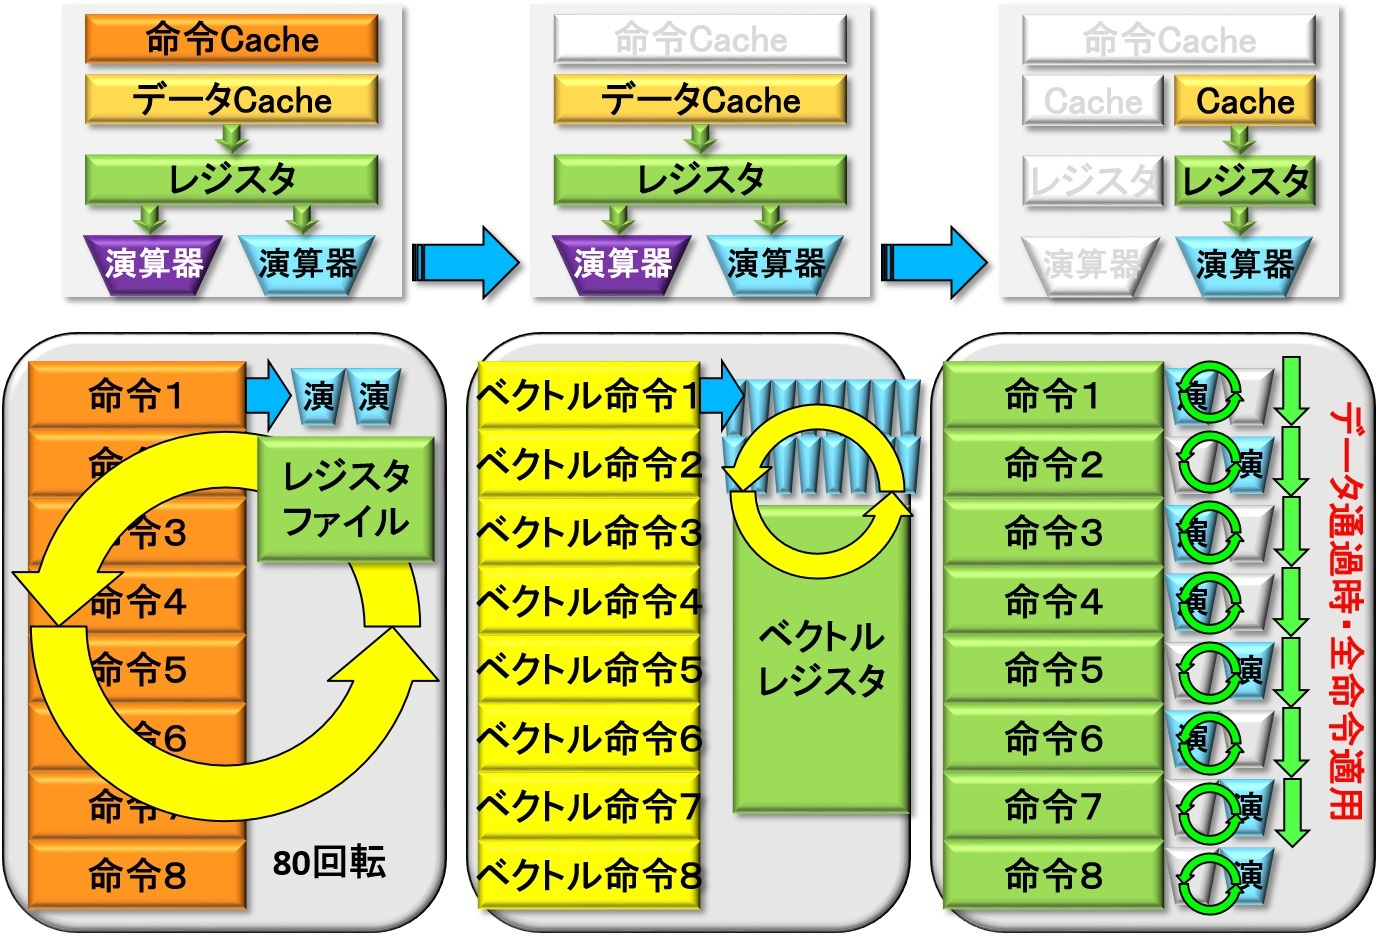
\includegraphics[angle=270,origin=b,width=0.70\textwidth]{CGRA0.eps}
\caption{\label{cgra0}Difference between CPU/GPU and CGRA on execution model}
\end{figure}

\begin{figure}[htbp]
\center
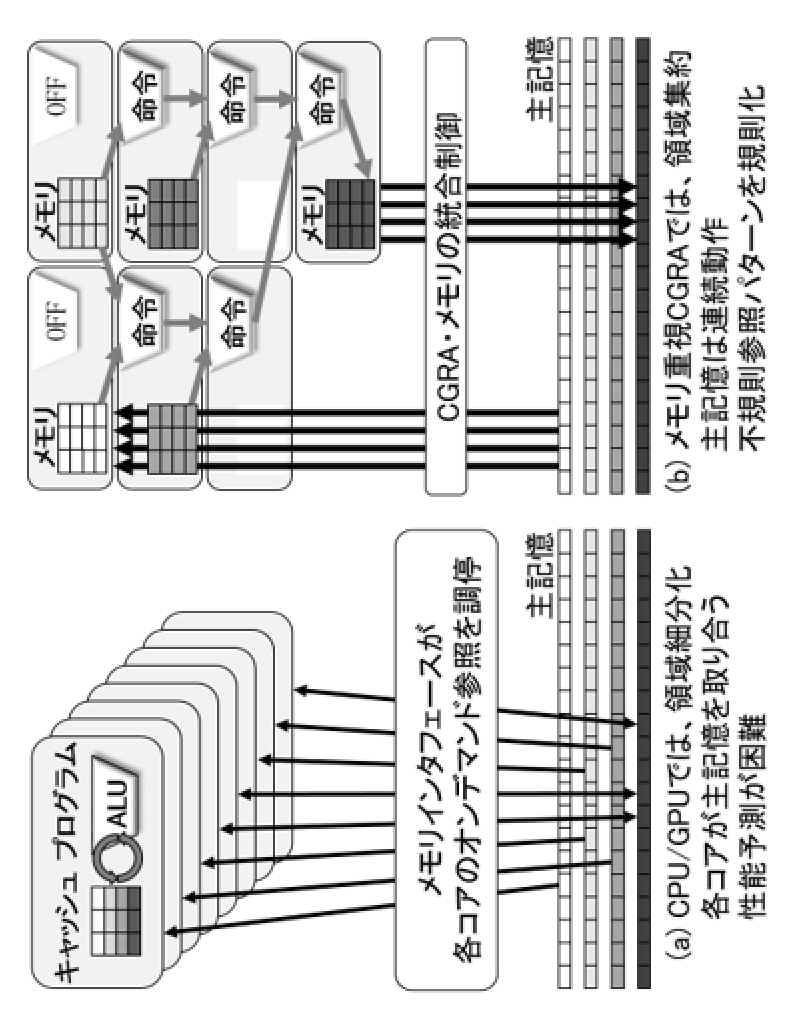
\includegraphics[angle=270,origin=b,width=0.60\textwidth]{gpu.eps}
\caption{\label{gpu}Difference between CPU/GPU and CGRA on memory access}
\end{figure}

The von Neumann-type computing platform, in which machine instructions sequentially control the arithmetic unit and memory, has been supported by the two wheels of semiconductor miniaturization and parallel processing sophistication.  The former approached the physical limit and the latter was pursued.  GPGPU is equipped with a large-scale register file and a main memory delay concealment function that exceeds 1000 cycles by multithreading in order to perform parallel processing while maintaining conventional programmability.  However, tuning to regularize the main memory reference order is difficult, and excessive computing power and power are required to achieve the required performance.  On the other hand, the Coarse Grain Reconfigurable Architecture (CGRA) proposed by H.T.Kung et al. in 1982 is a non-Von Neumann type that maps the instruction sequence of the innermost loop to a two-dimensionally arranged arithmetic unit network and flows the main memory data.  While many domestic companies have started but withdrew due to programmability barriers, Google's TPU and Wave computing's DPU have succeeded in improving efficiency by focusing on AI applications.  Our laboratory developed a VLIW-compatible LAPP in 2008, and then developed IMAX, which dramatically improved area efficiency (calculation performance/area) by integrated control of 64 sets of near-memory high-performance arithmetic units and multiple loops.  While GPGPU employs a large number of cores in SIMD and requires coalescing that integrates memory references into continuous addresses and a luxurious memory bus, IMAX employs a large number of arithmetic units to be connected vertically to the memory bus.  We have achieved power reduction.
 
\begin{figure}[htbp]
\center
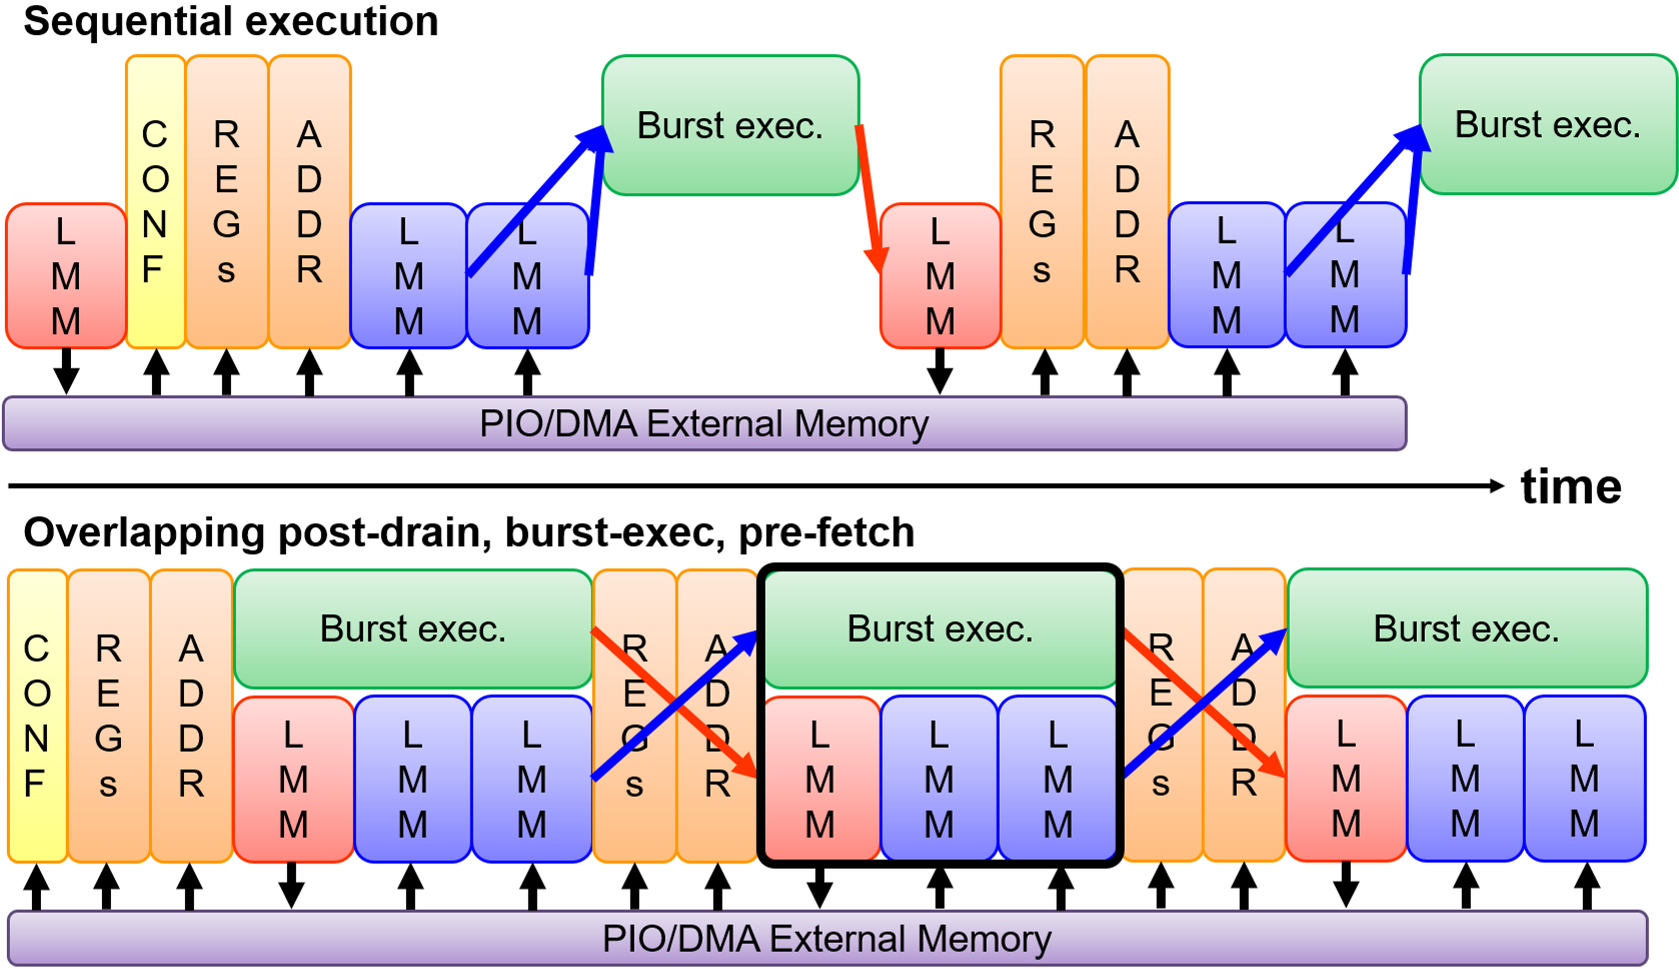
\includegraphics[angle=270,origin=b,width=0.60\textwidth]{cgra.eps}
\caption{\label{cgra}Ideal operation of CGRA}
\end{figure}

\begin{figure}[htbp]
\center
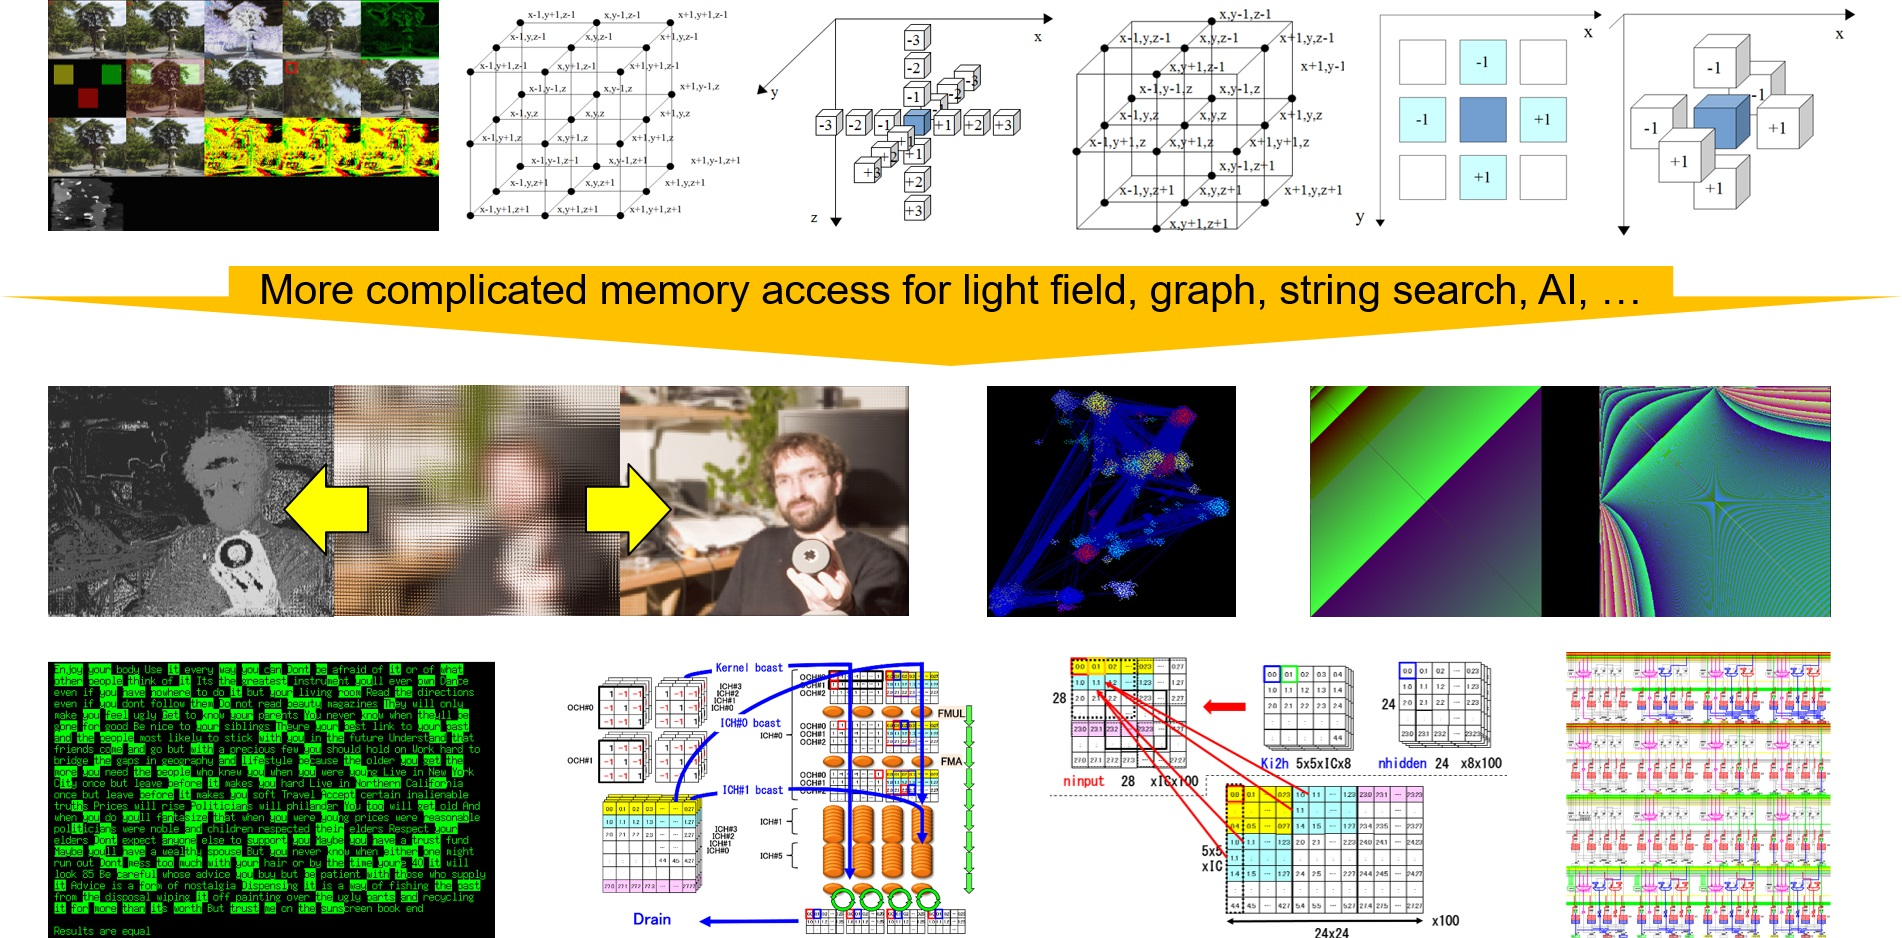
\includegraphics[angle=270,origin=b,width=0.98\textwidth]{APPL.eps}
\caption{\label{appl1}Complicated applications}
\end{figure}

\begin{figure}[htbp]
\center
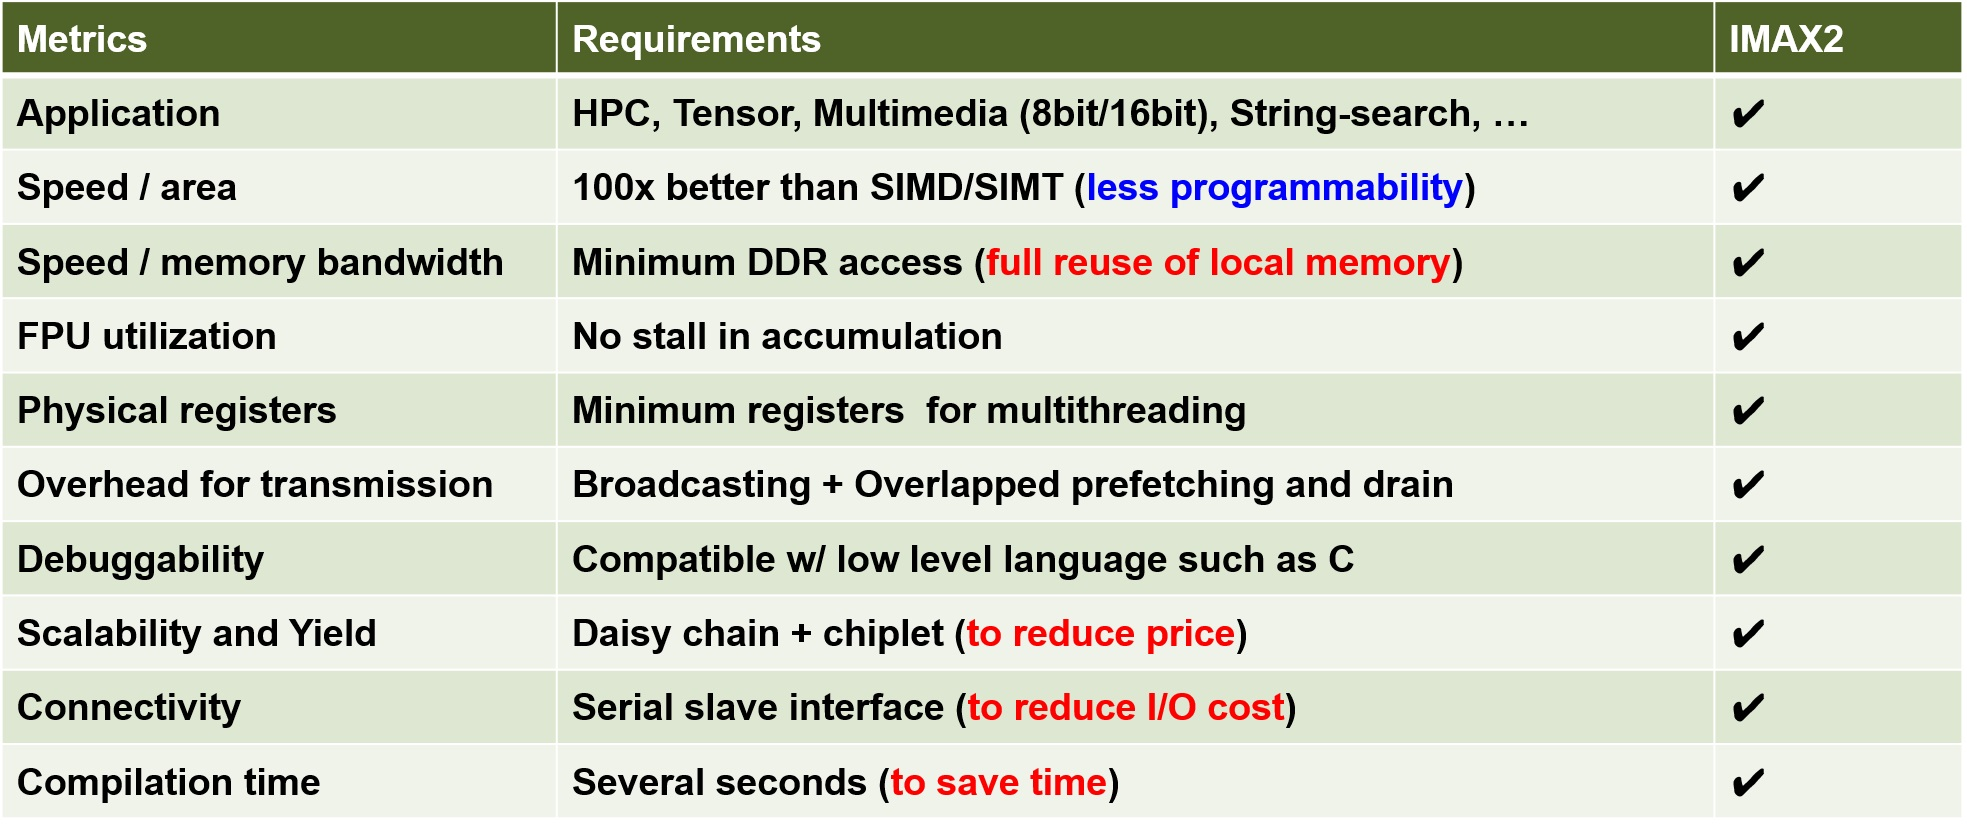
\includegraphics[angle=270,origin=b,width=0.98\textwidth]{LIST.eps}
\caption{\label{list1}Requrements on CGRAs}
\end{figure}

The CGRA is a mechanism that executes a huge number of operations at one
time. To use it efficiently, as shown in Fig. \ref{cgra}, the last operation
result is flushed to the main memory, the operation is performed, and the
next operation is performed. It is extremely important to keep the operation
unit running by overlapping the fetching of the data required for the
operation from the main memory. In addition, application programs are
becoming more complicated as shown in Fig.\ref{appl1}.  Many features shown
in Fig.\ref{list1} should be supported by CGRAs.

\begin{figure}[htbp]
\center
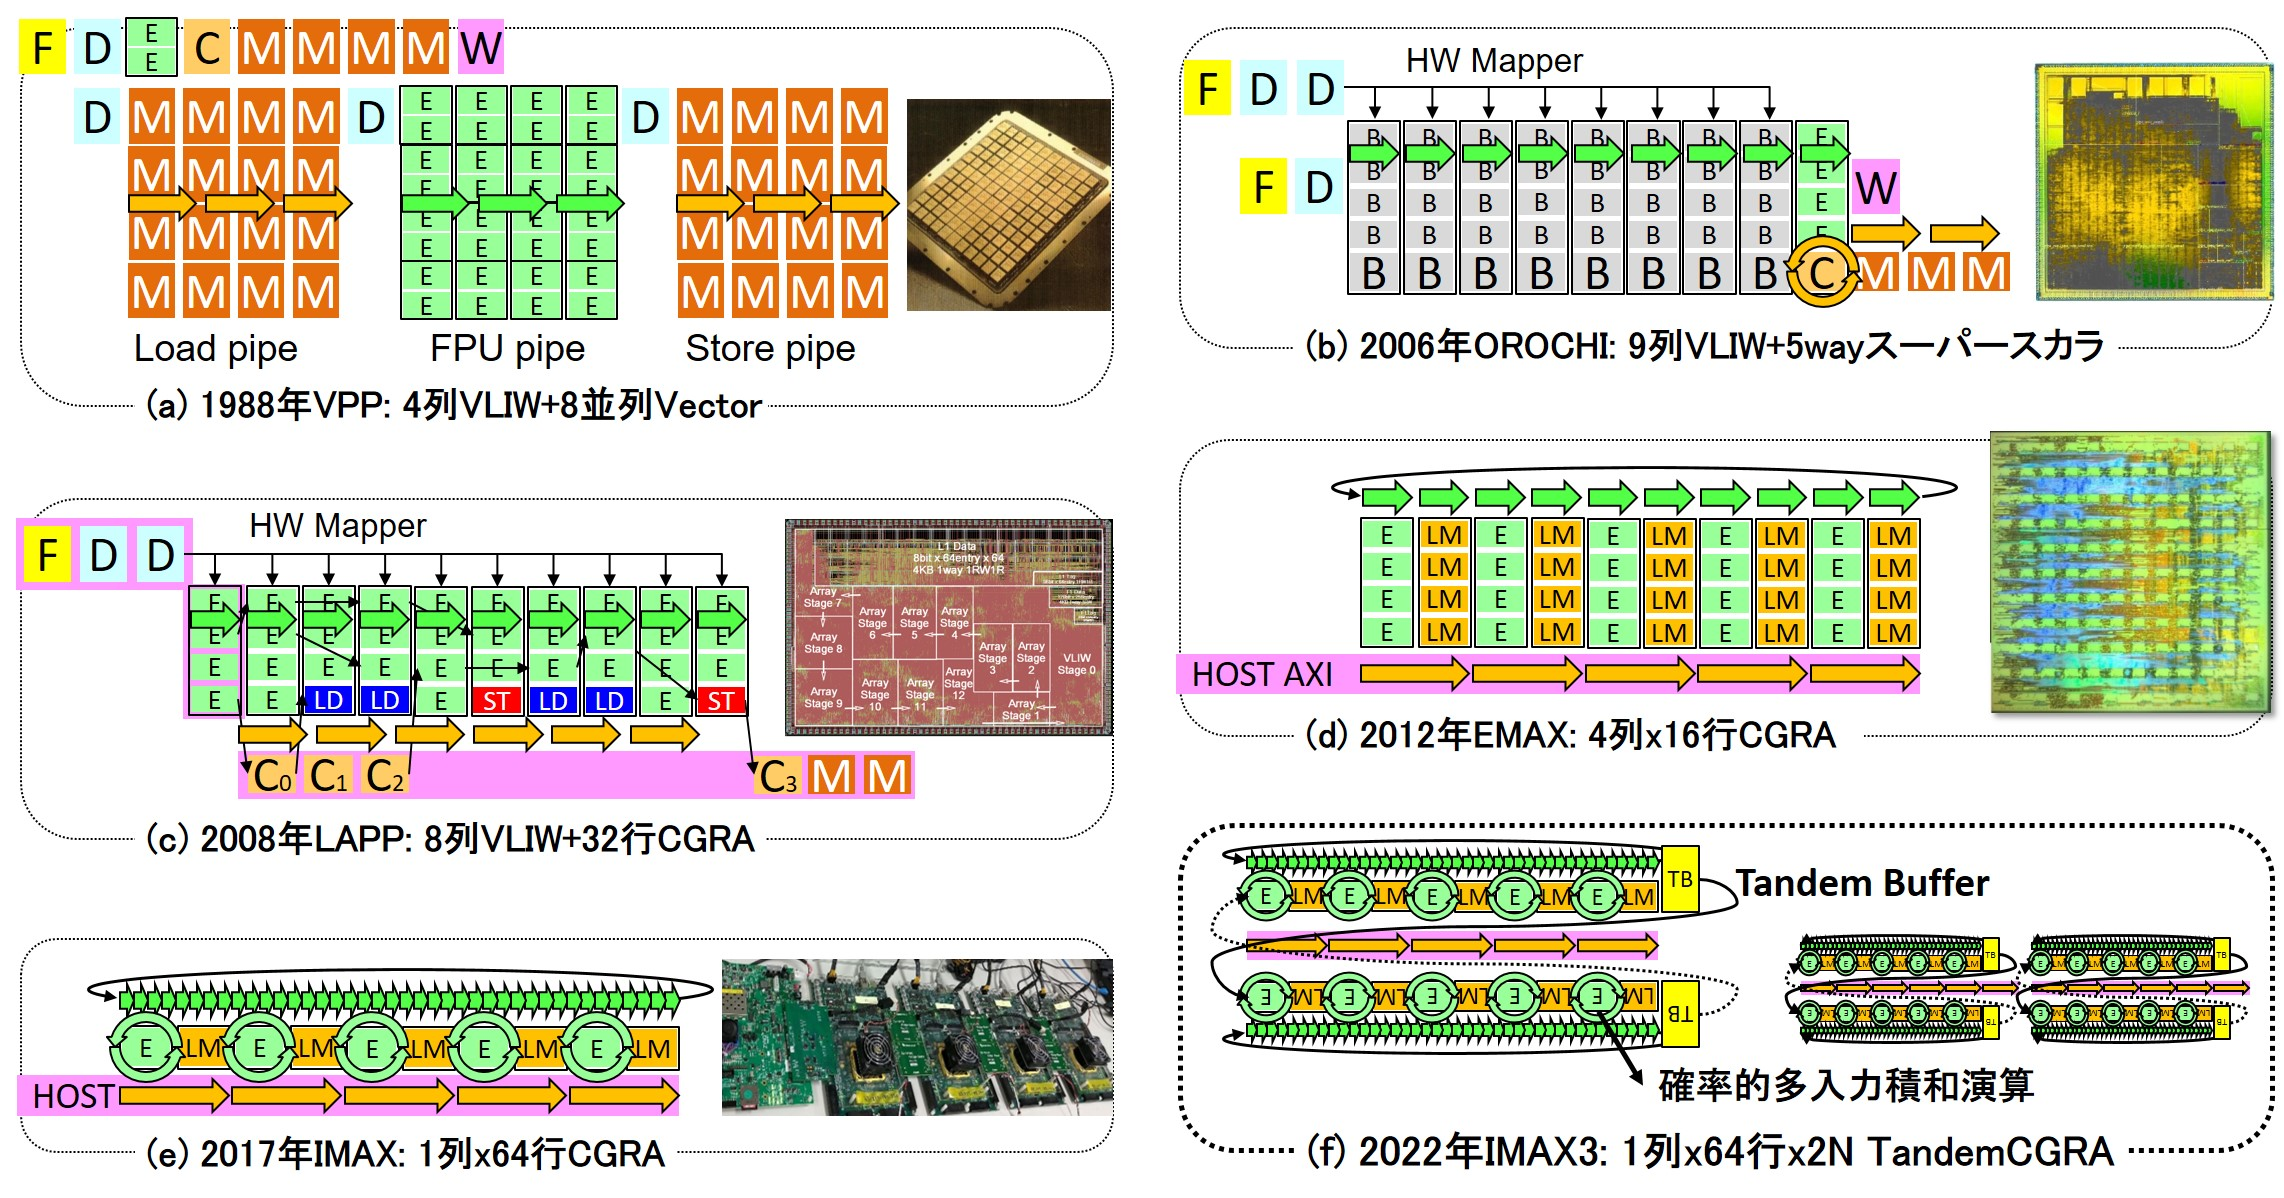
\includegraphics[angle=270,origin=b,width=0.98\textwidth]{CGRA1.eps}
\caption{\label{cgra1}VPP-IMAX history of execution model}
\end{figure}

\begin{figure}[htbp]
\center
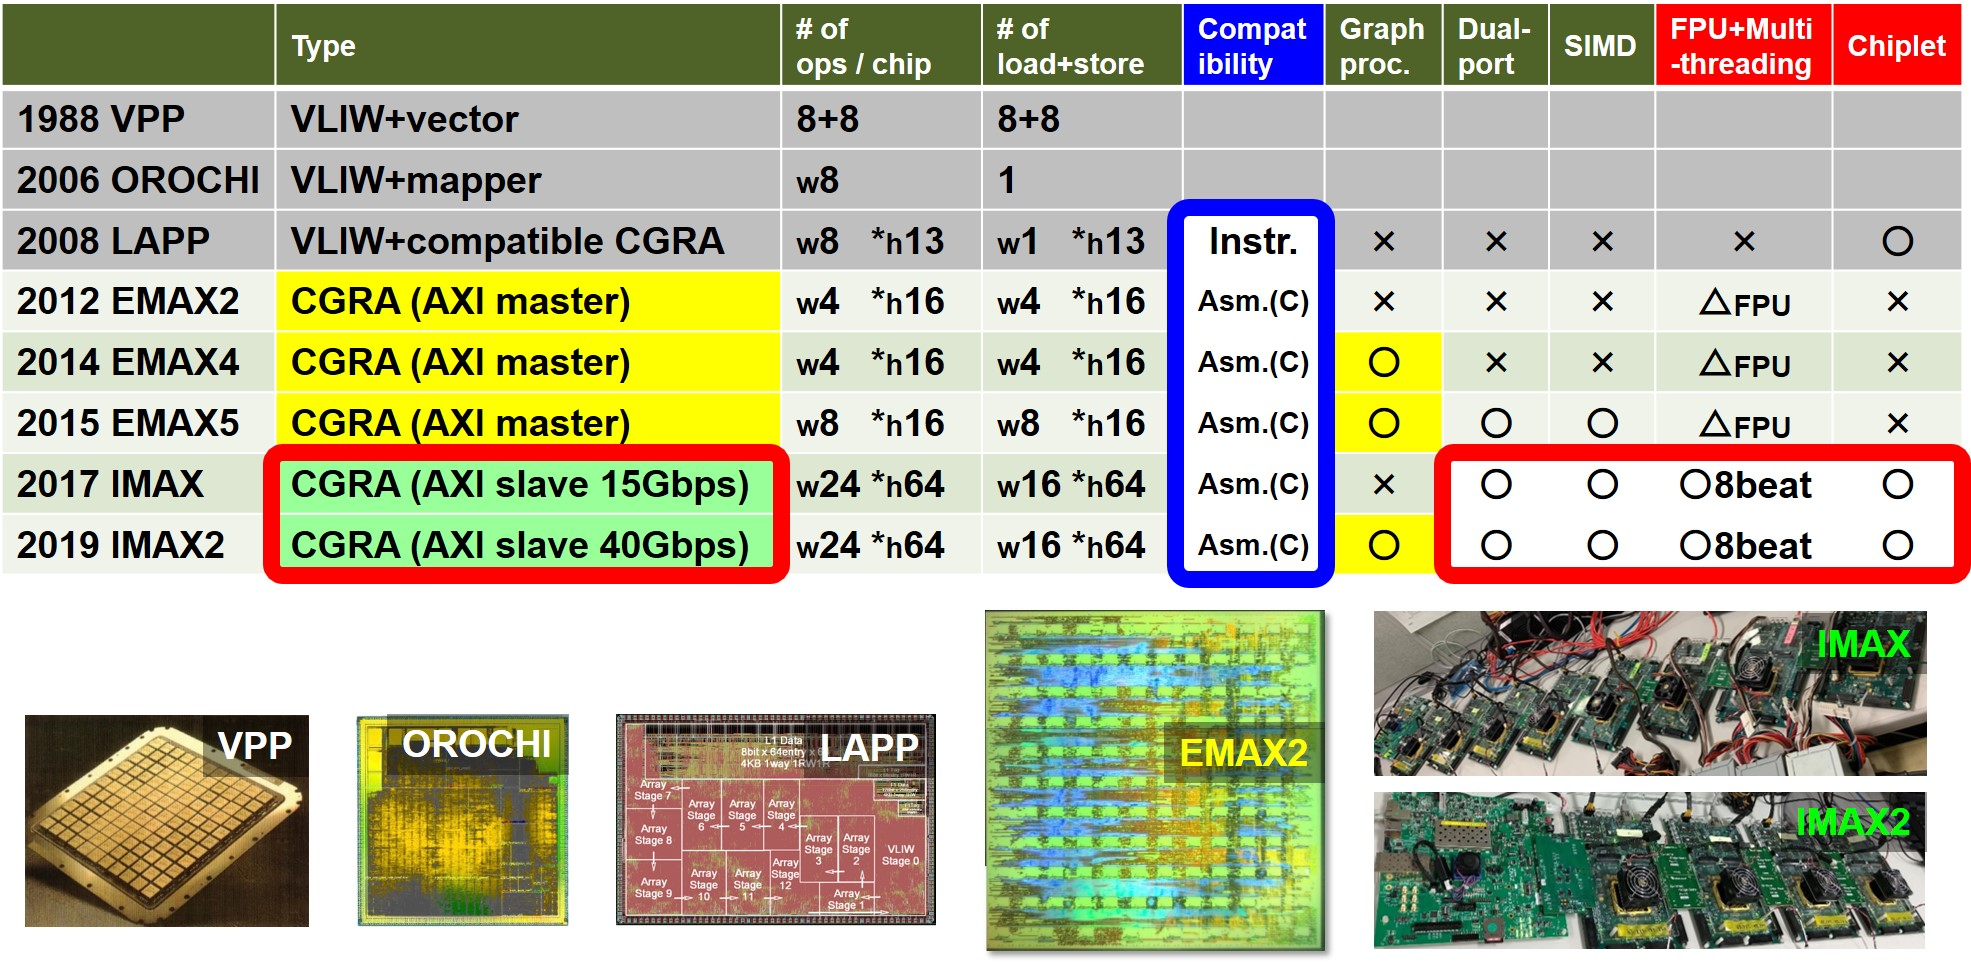
\includegraphics[angle=270,origin=b,width=0.98\textwidth]{HISTORY.eps}
\caption{\label{history1}VPP-IMAX history of features}
\end{figure}

The process leading up to IMAX is shown in Fig.\ref{cgra1} and
Fig.\ref{history1}. In the (a) parallel vector VPP series, VLIW was proposed
and adopted to maximize power efficiency while overseas manufacturers were
leaning toward superscalar processors. The VLIW + vector arithmetic
mechanism has the feature that the continuous operation of the memory pipe M
and the arithmetic pipe E is very similar to CGRA, but there are no
structural restrictions on the program. (b) OROCHI is a VLIW shared
low-power superscalar in which the instruction decoder D dynamically
decomposes and inputs ARM instructions into the VLIW buffer B and shares the
cache C. The CGRA configuration technology by two-dimensional extension of
VLIW was demonstrated, and (c) LAPP, the first VLIW compatible CGRA,
inherited it. (d) After EMAX, the efficiency of discrete stencil calculation
and graph processing has been improved by maximizing the reuse of LM by ring
connection between arithmetic unit E and local memory LM and eliminating
data flow interference by explicit control. At the same time as Google's TPU
(integer operation only), (e) IMAX employs multiple execution that
virtualizes 1 physical column x 64 rows into 4 logical columns x 64 rows,
and the maximum reuse of LM. The area efficiency (calculation performance /
area) of the arithmetic floating-point multiply-accumulate operation E has
been dramatically improved (250 times the built-in GPGPU assuming 28
nm). (f) Tandem CGRA is a configuration that improves programmability by a
virtualization mechanism.

\clearpage

\section{History of CGRA}

\begin{figure}[htbp]
\center
\epsfile{file=CGRAHIST1.eps,width=0.95\textwidth}
\caption{\label{cgra2}LAPP-IMAX history of ALU network}
\end{figure}

Figure \ref{cgra2} shows the structure of one line of the CGRA developed by
our group. LAPP was a VLIW compatible CGRA, but the local memory (LMM)
capacity of each row composed of FIFO was as small as 16 elements x 4
columns at most, and it could not handle stencil calculations with large
orders (length of one side). In EMAX2, instead of abandoning VLIW
compatibility, a dedicated medium-capacity LMM and FIFO were placed in each
arithmetic unit so that many stencil calculations could be mapped. However,
increasing the number of LMMs greatly increased the number of interline
registers to 32. Therefore, four cycles were required from the register to
the output of the computing unit.  In EMAX4, a transaction mechanism
required for graph processing was added. The changes from EMAX2 to EMAX4 are
as follows:

\begin {itemize} \parskip 0pc \itemsep 0pc
\item Add conditional execution by combining multiple conditions
\item Add transaction function
\item Data bus between each stage and external memory is expanded from 64bit * 1 to 32bit * 4
\end {itemize}

In EMAX5/L2, a SIMD operation mechanism was added, and the input registers
of ALU and EAG were shared, reducing the number of inter-line registers by
half to 16. From registers to the output of the arithmetic unit takes 2
clock cycles. Also, the throughput between the external memory bus and the
LMM has been improved.  In EMAX5/ZYNQ, the FIFO was deleted to reduce the
FIFO initialization overhead. Instead, a path has been added to write data
from the external memory bus to multiple rows of LMMs simultaneously. This
made it possible to initialize many LMMs simultaneously using multiple
external memory buses. The changes from EMAX4 to EMAX5/ZYNQ are as follows:

\begin{itemize}\parskip 0pc \itemsep 0pc
\item SIMD conversion from single-precision floating-point operation to 32-bit * 2 operation
\item SIMD conversion of 32bit integer operation to 32bit * 2 integer operation
\item Enhanced 8/16bit media operation from 4/2 width SIMD to 8/4 width SIMD
\item The local memory (LMM) bus width of each module has been expanded from 32bit*1 to 64bit*4, and the throughput between LMM and external memory has been increased by 8 times.
\item The connection between each stage and external memory has been expanded from 32bit * 4 * 1 channel to 64bit * 4 * 4 channel, and the throughput between each stage and external memory has been increased by 8 times (conf / regv / lmmi initialization overhead (Reduced to 1/8)
\item Adoption of Dual-Port-LMM for direct reference to external memory and change of basic configuration of CGRA
\item Inter-unit bus network that can output data to LMM while supplying data from 3 units of LMM to 3-input SIMD
\item Reduce the number of propagation registers per unit from 8 to 4, and place a crossbar switch from propagation registers to arithmetic units.
\item The FIFO that propagates the output of the LMM in the horizontal direction is deleted, and a mechanism for broadcasting from the external memory bus to the LMM in the same stage is provided instead (FIFO initialization is not required).
\end{itemize}

In IMAX, in order to improve the large number of wirings, which are common
drawbacks of the CGRA, and the low operation circuit usage rate during
self-loop operation, we introduced multithreading, which bundles
multiple-column arithmetic functions into one column. Multithreading can be
implemented thanks to the fact that there is no dependency on the horizontal
operations.  By implementing a multi-column arithmetic function (logical
UNIT) logically and physically implementing it with a single-column group of
arithmetic units, it is possible to reduce the number of arithmetic units
and wiring, improve the efficiency of arithmetic units, eliminate the need
for horizontal broadcasting, and eliminate the need for redundant LMMs.  In
addition, the method of connecting to the CPU was changed to AXI-SLAVE, and
writing to the LMM was changed to a method in which each UNIT is
autonomously imported according to the vAddr-range provided for each
UNIT. This enabled vertical broadcasting. Furthermore, by adding a path that
returns the output of the UNIT to the input, read-modify-write for the same
LMM was enabled, and the LMM accumulation required for convolution operation
and inverse matrix calculation was enabled. By setting a continuous
vAddr-range for multiple rows of LMMs and performing the same store for
multiple LMMs, it became possible to increase the accumulation space several
times. The changes from EMAX5/ZYNQ to IMAX are as follows:

\begin{itemize}\parskip 0pc \itemsep 0pc
\item Reduce the number of physical computing units and LMMs while maintaining program compatibility with EMAX5/ZYNQ
\item Improvement of HOST - LMM transfer efficiency by AXI-SLAVE, lmring 8 rows and 8 columns configuration, and vertical broadcast function
\item Read-modify-write function and accumulation function using the same LMM
\item Tandem mode of units employing double buffering in LMM (for FFT and multistage merge sort)
\item Read-data comparator and address incrementor in dual port LMM (for multistage merge sort and sparse MM)
\item Sparse matrix multiplication of compressed elements including location information
\item Multi-loop batch execution function including multi-chip support and mapping to multi-chip
\item Multiple transaction unification (AXI4 conversion) and buffering function to accelerate DMA-READ of AXI3 with burst length of up to 8 (in case of 256bit width)
\item Unaligned 64bit-load employing dual EAG
\item Duplicating 32bit/8bit-load to 64bit register for SIMD
\item Dynamic DMA concatenation for multiple LMM
\end{itemize}

\section{Policy of IMAX}

The conventional CGRA has an essential weakness, and it is not
suitable for a small accelerator contributing to the edge as it is.  The
problems can be seen as follows:

(1) Long-distance wiring or wiring congestion causes a decrease in operating
frequency and area efficiency when mounted with a two-dimensional lattice
structure, so that a measure for area saving is required. (2) It is
necessary to have a mechanism that does not hinder pipeline execution even
if there is an instruction that essentially requires multiple cycles, such
as a floating-point accumulation operation or read-modify-write to a local
memory. (3) The speed of the innermost loop alone is not suitable for
speeding up the matrix product with a short vector length or the speed of
the convolution operation. Therefore, a multi-loop batch execution function
for reducing startup overhead is required. (4) In order to increase the
reuse efficiency of the local memory and reduce external memory references,
an instruction mapping position shift function (that can follow the
fluctuation of the data reference pattern, which is difficult to perform
static analysis) is required. (5) High efficiency can be achieved as a
simple DMA slave memory without the need to incorporate a sophisticated DMA
master function. (6) Scalable performance can be easily obtained by
cascading utilizing the function of the slave memory without the need for an
additional external memory bus (AXI).

In IMAX, the \textbf{first point} is that: \textbf{it is NOT the
two-dimensional configuration} generally known by the traditional CGRA. To
fulfil low cost requirement for IoT edge device, \textbf{the physical
structure of this architecture is one-dimensional (linear array)}. However,
it must still maintain high performance as the traditional two-dimensional
architecture does. \textbf{The second point: It integrates the memory
function inside}. Since the host uses it as memory, it can deal with the
problem of memory-memory transferring overhead in traditional
accelerator. In addition, the internal memory can be cascade easily.
\textbf{The third point: Various data paths are provided} for intuitive
programming that handling the integrated of memory functions and arithmetic
functions. In particular, \textbf{this architecture allows read-modify-write
and multiple loop control on the same local memory}, which ordinary CGRAs
cannot.  \textbf{The fourth point}: Thanks to the carefully designing the
data path, \textbf{compiling speed of EMAX 6 is high.} It does not require
exploratory compilation such as normal FPGA.

\begin{figure}[htbp]
\center
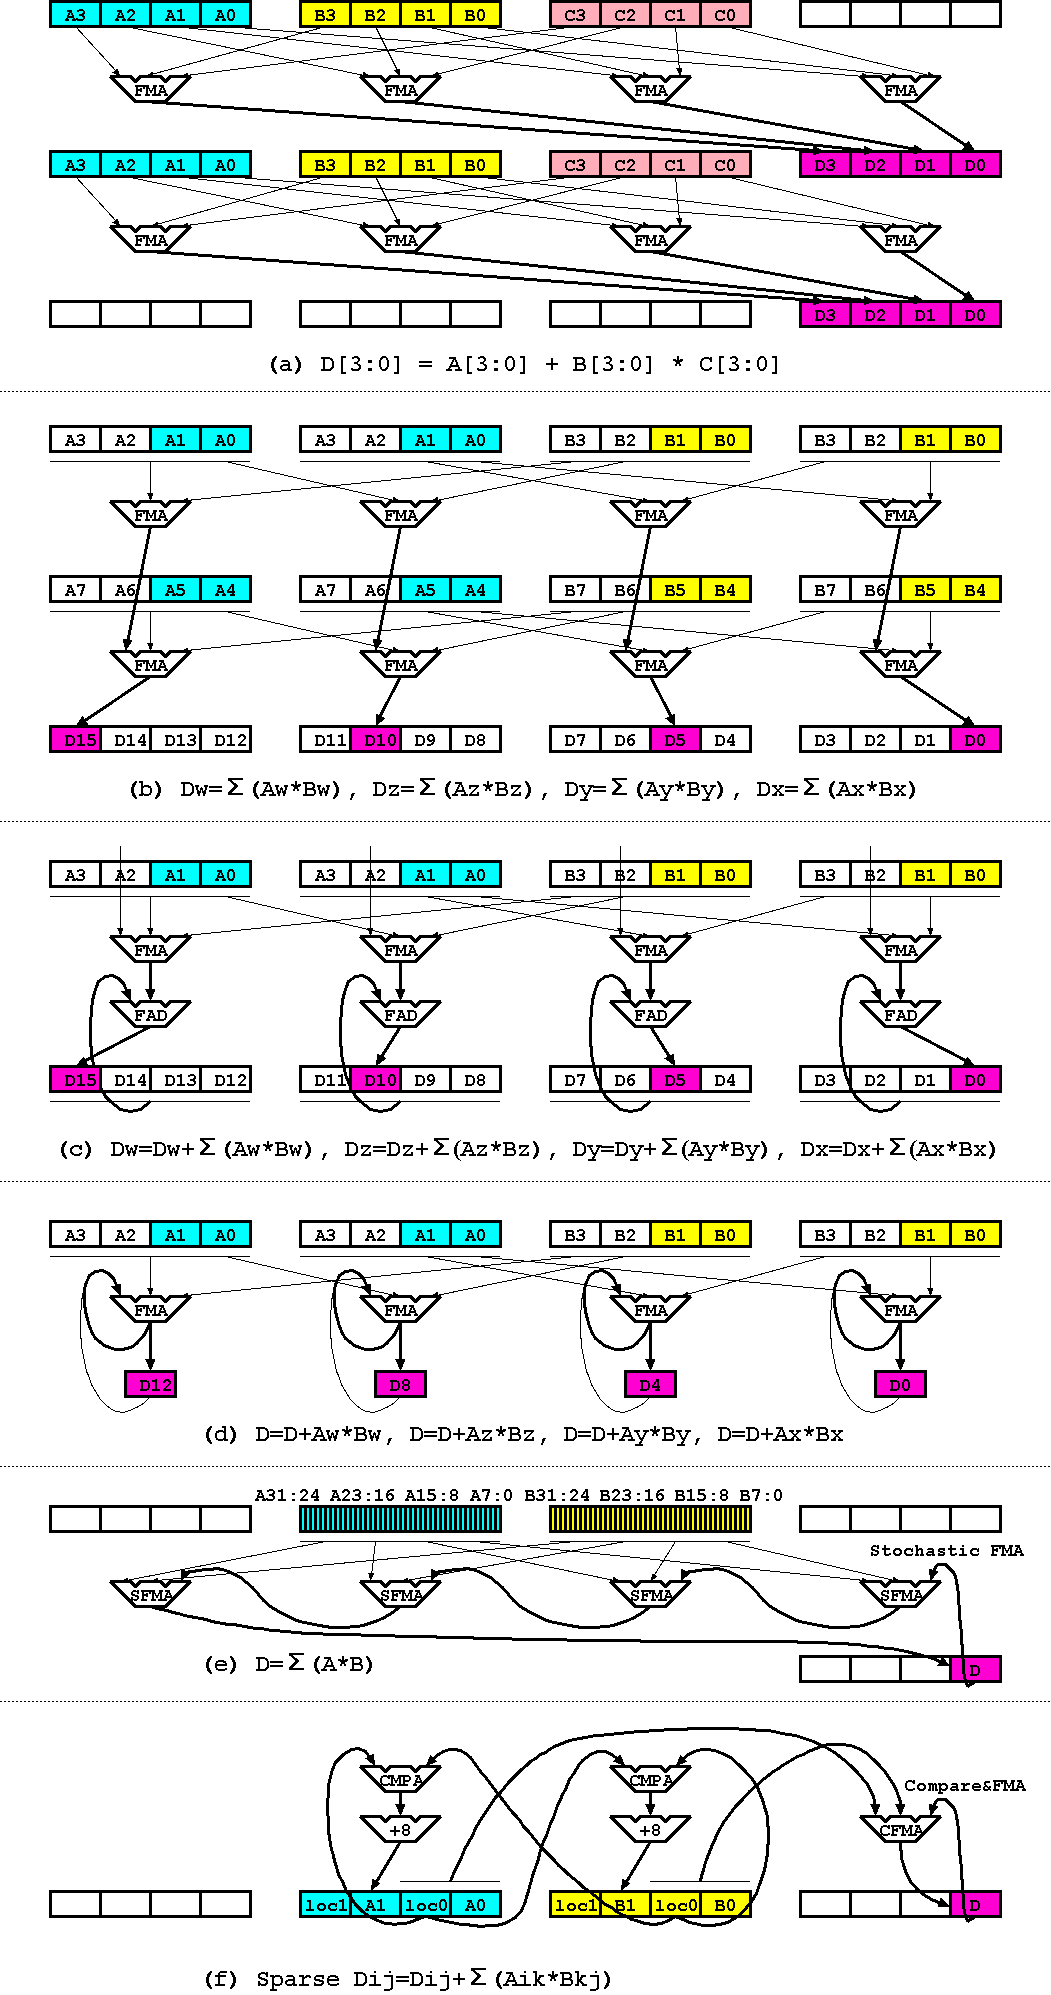
\includegraphics[angle=270,origin=b,width=0.98\textwidth]{EMAX6EXP.eps}
\caption{\label{exp}Requirements on memory access patterns}
\end{figure}

On IMAX, a maximum of 10 instructions (2 operations x 3 stage + load x 2 +
store x 2) x 4 columns x 64 rows = 2560 instructions can be mapped at a time
to a physical structure of 1 column x 64 rows.  IMAX has a physical
structure in which basic units are arranged in one column x 64 rows
(described later), but the hardware model at the time of programming is 4
columns x 64 rows.  Each unit has two sets of three-input single-precision
floating-point adder / subtract or multipliers of a three-stage pipeline,
and executes two operations simultaneously using 64-bit wide registers.  The
first stage of the pipeline can perform various multimedia operations and
fixed-point operations in 8/16/32-bit units, the middle stage can perform
logical operations, and the last stage can perform shift operations.  Each
unit has 64KB dual port memory, as shown in Figure \ref{exp}. It can handle
various memory reference patterns.

In (a), A, B, and C stored in one row of local memory (LMM) are read out
four words at a time, SIMD calculation is performed by four calculators, and
the calculation result D is stored in the next-stage LMM. This is a state in
which two sets are mapped.  A, B, and C are supplied from external memory,
and D is retrieved to external memory.  (b) is a map that performs vertical
convolution. A and B were supplied from the dual port memory to the
arithmetic units in each column, and four convolution operations were
performed.  (c) is a mapping that accumulates four D's in the LMM.  Unlike a
typical CGRA, accumulation can be performed while propagating data
downstream as a whole.  (d) is a mapping that similarly accumulates four
systems of D in the LMM.  However, it corresponds to the case where the
storage destination is fixed and the LMM is updated many times by
read-modify-write.  (e) is an extension for in-unit MAC with multiple input.
(f) is an extension for sparse matrix multiplication and merge sort
<
\begin{figure}[htbp]
\center
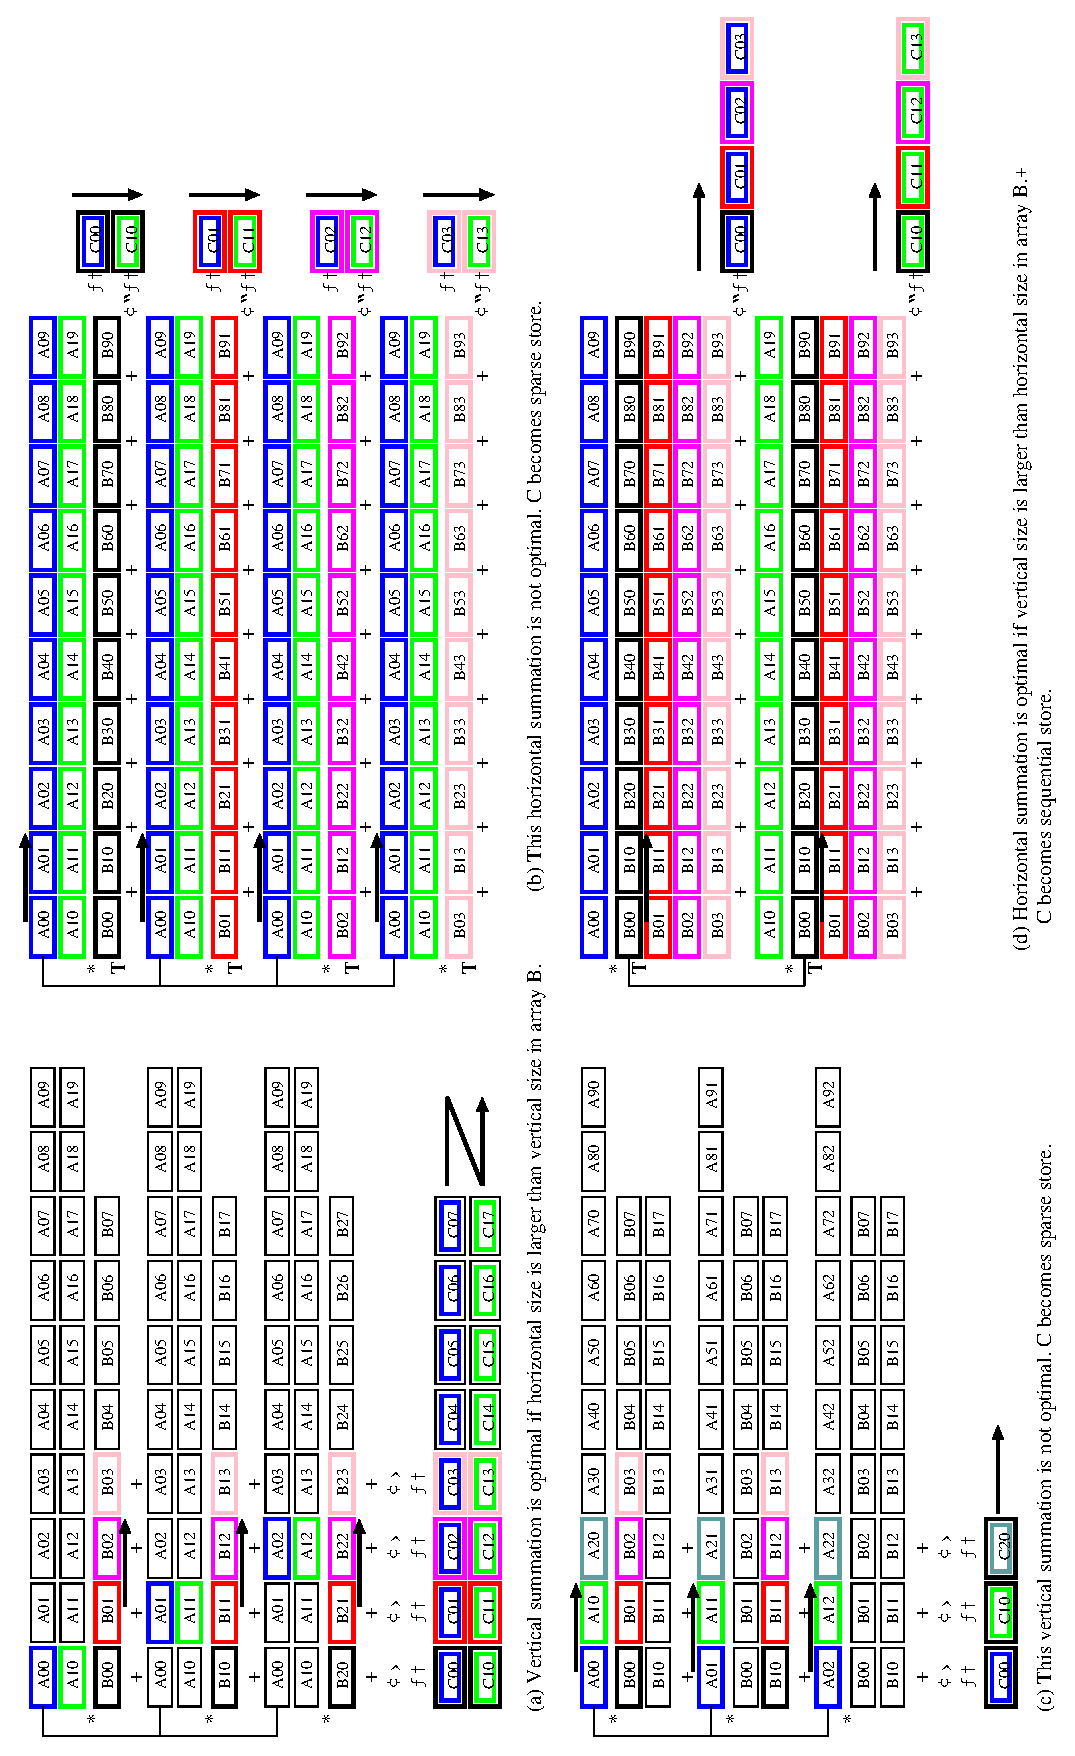
\includegraphics[angle=270,origin=b,width=0.98\textwidth]{CGRAPAT.eps}
\caption{\label{fig:cgrapat}Optimal direction of summation in matrix multiplication}
\end{figure}

For example, in case of matrix multiplication, the optimal direction of
summation depends on the shape of the matrix B as shown in
Fig.\ref{fig:cgrapat}. For vertical (a), Fig.\ref{exp}(b) and
Fig.\ref{exp}(c) are required. The (b) is not optimal due to coarse store to
C. Also the (c) is not optimal due to coarse store to
C. For horizontal (d), Fig.\ref{exp}(d) or Fig.\ref{exp}(e) is required.
Although the difference is that (a) broadcasts multiple rows of array A in
vertical direction and (d) broadcasts multiple rows of array B in vertical
direction after transpose, the store addresses in C become sequential.

\section{Column direction multi-threading to save area}

\begin{figure}[htbp]
\center

\includegraphics[angle=0,origin=b,width=0.98\textwidth]{unit.eps}
\caption{\label{fig:unit}Column multithreading for small footprint and
bubble-free execution}
\end{figure}

Column-wise multithreading was introduced to address issues (1) and (2).
Figure \ref{fig:unit} (a) shows the general unit configuration.  In general,
CGRAs are designed on the premise that each operation unit outputs
the operation result every cycle in order to reduce the synchronization cost
with its previous and following operations. For this reason, functions with
long operation time such as floating point accumulation cannot be pipelined,
and area efficiency deteriorates.  In addition, in order to perform a large
number of readings from the LMM, it is necessary to arrange multiple LMMs
holding the same contents to increase the number of ports, which is a factor
of area efficiency deterioration.  Figure \ref{fig:unit} (b) shows the unit
configuration after applying multi-threading (W = 4). One unit logically
implements the same function as (a), and it needs 4 cycles for calculation.
When the arithmetic unit is pipelined into four stages, including the
16-to-1 selector that selects Reg \# 0-15, and four operations in the
horizontal direction are time-divided, the same performance can be
maintained even with the floating-point accumulation, and the area
efficiency can be improved by a factor of four.  However, in (a), the
operation delay time in one unit is 2 cycles, whereas in (b), it is 8
cycles.  Also, in order for the next-stage unit to refer to all of the
operation results and LMM read data of the previous-stage unit (that can be
output over four cycles), Reg \# 0-15 double buffering is required (grp.A
and grp.B).  For the LMM, if the port is made into eight ports by the
four-cycle operation of the two-port LMM, the area efficiency can be
improved by a factor of four when all four LMMs in the horizontal direction
have overlapped.  When there is no overlap, the efficiency of the memory
itself does not change because the capacity of the LMM is divided and used,
but the number of address generators can be reduced.  AXI-WRITE-IF and
AXI-READ-IF refer to the LMM using a cycle in which the data path for
operation does not use the load/store port of the LMM.

\begin{figure}[htbp]
\center
\epsfile{file=CGRAHIST2.eps,width=0.98\textwidth}
\caption{\label{cgra3}Double buffering of registers is important in IMAX}
\end{figure}

Figure\ref{cgra3} shows the importance of double buffers in IMAX.  (a) is the
relationship between the memory and ALU in a normal CGRA
with 4-column configuration.  A 3-read 1-write memory is required to read
4 words from each of the 3 locations in the memory and write the output (4
words) of 4 arithmetic units operating in parallel to the memory.  In the
case of a floating-point unit with 4-stage pipeline
configuration, throughput does not decrease if there is no dependency
between addresses, but if there is a dependency such as accumulation, the input
waits for its own calculation result, so the pipeline stops and the
performance drops to 1/4.  In order not to stop the pipeline, it is
sufficient to make it 4-way-multithreading using only one ALU as
shown in (b).  However, even if the number of arithmetic units can be
reduced, the number of memory ports cannot be reduced.  (c) is a
configuration in which SIMD-LD is revived to reduce the number of ports.
The program is described as a set of SIMD-LD, SIMD-FMA, and SIMD-ST.  The
hardware uses 3 out of 4 cycles to read from 3 locations with SIMD-LD.  Once
saved in the double buffer, the 3 inputs required for each operation can
always be available in all 4 cycles.  SIMD-FMA is executed by
multithreading, and the calculation results are stored in memory in order.
In other words, SIMD-FMA and SIMD-ST do not actually operate as SIMD, but the
performance of hardware can be fully extracted.

\begin{figure}[htbp]
\center

\includegraphics[angle=0,origin=b,width=0.60\textwidth]{rmw.eps}
\caption{\label{fig:rmw}Read-modify-write operation}
\end{figure}

Figure \ref{fig:rmw} shows the correspondence of read-modify-write operation
with unit.  Logically, four columns of read-modify-write are physically
mapped to a single unit. The accumulation result (sum0-3) by the previous
stage arithmetic unit is sent to the lower register of the unit. The result
of the load (o0-3) is fed back to the input of the operation unit in
synchronization with the timing, and the addition result (s0-3) is stored in
the LMM.

\section{Batch execution of multiple loops}

\begin{figure}[htbp]
\center 
\includegraphics[angle=0,origin=b,width=0.80\textwidth]{loop.eps}
\caption{\label{fig:loop}Multilevel loop control}
\end{figure}

To cope with issues (3), multiple loop batch execution was introduced. Since
CGRAs require instruction mapping and register initialization before
starting continuous execution, we want to increase continuous execution time
and reduce startup overhead as much as possible. However, the continuous
execution time is determined by the amount of data that can be stored in the
LMM, and the capacity of the LMM has an upper limit for not decreasing the
operating frequency of the pipeline arithmetic unit. Experimentally, the LMM
that balances with a single-precision floating-point operation pipeline
consisting of three stages is about 32 KB (the former vector operation
mechanism was up to about 16 KB per vector register). 16K cycles divided by
the number of words (4B) that can be stored in 64KB is the upper limit of
the continuous execution time. In the Lightfield (LF), the input is 8K
images, so the LMM can be used up enough. On the other hand, in the case of
Matrix Multiplication (MM), the col corresponding to the continuous
execution time is M/W (120 when M = 480, W = 4). It is extremely short in
case of Convolutional Neural Network (CNN), which is M-2 (240 for M =
242). In order to use LMM as much as possible, MM is a double loop with a
row loop of rotation speed GRP = 8 inserted outside, continuous execution
time is M/WxGRP = 960, and CNN is also GRP = 8 and (M-2)xGRP = 1920.  A
multi-loop batch execution mechanism is also added to the hardware.

Figure \ref{fig:loop}(a) is the actual C code at the top of the CNN, and (b)
is a logical multiplexing loop using a 4-column configuration (columns 3, 2,
1, and 0 from the left). The control method is shown. Lines 2 through 5 in
(a) are mapped to columns 1, 0, 2, and 3, respectively. Loop0, mapped to the
0th column, is the innermost loop counter involved in the continuous
execution of the CGRA. After the initial value M-2 is set in the register,
it is decremented by a self-loop every cycle and the result is nonzero. In
that case, leave the decrement value (initial value GRP) of loop1 mapped to
the first column as 0. When loop0 reaches 0, set M-2 to the left source of
column 0 again, switch the right source of column 1 to -1, decrement loop1,
set -4 to the left source of column 2 again, Switch the source on the right. 
Adding a row to the third column, M * 4, advances one iteration of
loop1. When loop0 and loop1 are both 0, continuous execution stops.  (c) is
the proposed method after column-wise multithreading is applied, and the
above control is performed by a single unit.  (b) Execute four operations in
parallel in one cycle.  On the other hand, (c) sequentially execute the
operations in the 0th to 3rd columns using 4 cycles of 4 times
frequency. The self-loop in the first stage of the pipeline arithmetic unit
handles data dependencies between columns. The multi-loop batch execution
mechanism includes read-modify-write function in the same LMM. The effect of
multi-loop batch execution is to accumulate the execution result and CNN of
the innermost loop stored in the LMM of the last stage of the MM by the
read-modify-write function without temporarily pushing out the DDR.

\section{Variety of LMM usage}

\begin{figure}[htbp]
\center
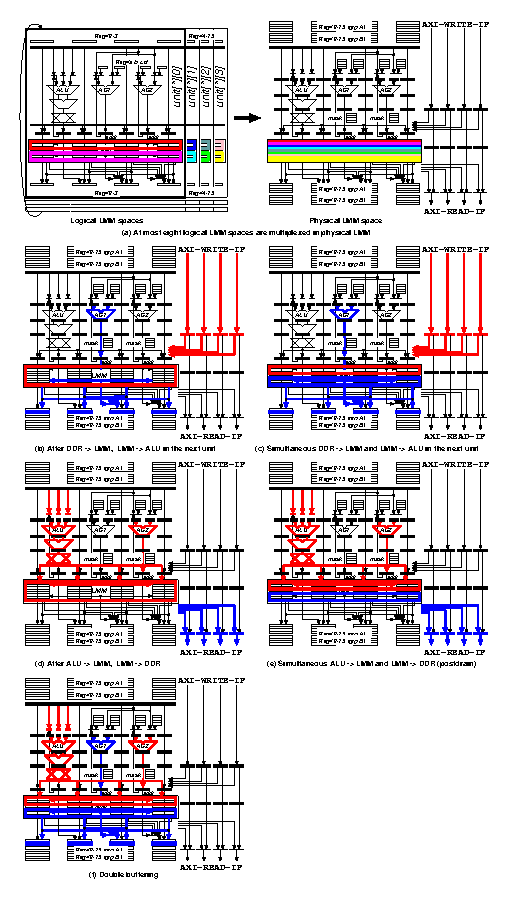
\includegraphics[angle=0,origin=b,width=0.85\textwidth]{lmmmode.eps}
\caption{\label{fig:lmmmode}Variety of LMM usage}
\end{figure}

Figure \ref{fig:lmmmode} illustrates vaiety of LMM usage.

\begin{description} \parskip 0pc \itemsep 0pc
\item{(a)} The physical LMM space can be divided into 4 corresponding to 4
logical columns, divided into 2 and shared by 2 logical columns, or shared
as a whole without being divided. Mixed division are also possible. When
using the prefetch/postdrain of the same LMM or the double buffering
function, the maximum number of partitions is 8.

\item{(b)} After reading the input data from the DDR to the LMM, the data is
supplied from the LMM to the ALU input. This is the normal usage of LMM when
load instructions are mapped. By combining prefetching to the adjacent LMM
and instruction mapping position shift, which will be described later, the
transmission time from DDR to LMM can be hidden in the execution time.

\item{(c)} The input data required for the next activation of IMAX is read
from DDR into another area of the same LMM while supplying prefetched data
from the LMM to the ALU input. Since the two spaces coexist in the LMM, the
DMA length is further halved after LMM space division.

\item{(d)} After writing the execution result to LMM, the output data is
written back from LMM to DDR. THis is the normal usage of LMM when store
instructions are mapped.  By combining the post-drain from the adjacent LMM
and the instruction mapping position shift described later, the transmission
time from the LMM to the DDR can be hidden in the execution time.

\item{(e)} While writing the execution result to the LMM, the previous
output data of the previous invocation is written back to the DDR from
another area of the same LMM.  Since the two spaces coexist in the LMM, the
DMA length is further halved after LMM space division.

\item{(f)} Data transmission between LMM and DDR can be suppressed by
specifying 0 as the DMA length. Furthermore, while writing a series of
calculation results to the LMM, the previous calculation result can be read
from the same LMM and used for the next calculation. In other words, LMM can
be used as a double buffer. It can be used for pipeline execution of
multistage processing such as FFT and merge sort.
\end{description}

\clearpage

\section{Ring formed interconnection among units and instruction mapping position shift function to reduce start-up overhead}

\begin{figure}[htbp]
\center
\epsfile{file=EMAX6RING.eps,width=0.90\textwidth}
\caption{\label{ring} Overview of 24-line configuration}
\end{figure}

To cope with issues (4), instruction mapping position shift function was
introduced. Figure \ref{ring} outlines a 24-line configuration including
DDR.  In EMAX5, the fsm (which in charge for each column) will performs
burst transfer between all LMMs and main memory that is connected by a
binary tree.  In IMAX, LMM is referenced by a pipeline memory bus. Since the
wiring for the binary tree can be reduced and the switching of the target
LMM is unnecessary, DMA transfer and PIO transfer can be mixed and executed
seamlessly.  In EMAX5, PIO can be used to initialize conf, lmmi, and regv,
which used only DMA. In IMAX, partial register updates can be speeded
up. The delay between UNITs during DMA transfer is 2 cycles, and the delay
between UNITs during operation execution is 8 cycles. The memory bus delay
time can be reduced by rearranging the memory bus from a 24-row per column
configuration to a multi-column configuration.

The instruction mapping position shift function is for reusing LMM without
moving data inside. The instructions are shifted by using the ring formed
interconnection among units.  The dynamic shifting revises the point that
conventional compilers always generated code of instruction shift before
starting continuous execution. Before starting continuous execution, it
compares the current LMM address range with the address range required for
the next continuous execution, and do not issue a shift instruction if they
are the same.

\section{Cascade connection function as memory}

\begin{figure}[htbp]
\center

\includegraphics[angle=0,origin=b,width=0.90\textwidth]{mchip.eps}
\caption{\label{fig:mchip}Cascaded peer-to-peer AXI bus for scalable multichip
CGRA}
\end{figure}

To address issues (5) and (6), a multi-chip configuration was devised. The
cost can be reduced by the multi-chip configuration because the yield is
improved by reducing the area of a single chip. It is new to remember that
AMD's Threadripper (4-chip MCM) is less expensive than Intel's Core-i9
(single chip).

IMAX uses ARMv8 as a host and can map any computing resources to the main
memory space of ARM as a memory device through the standard AXI bus. In this
case, it is possible to map multiple LMMs in one space and write images and
parameters to many LMMs at once by PIO/DMA from the host.  When describing
an application in C language, a programmer can specify which LMM is
associated with each data structure and arrange operations between the data
structures to form an arbitrary data flow. The data supply path has an 8
column x 8 row configuration to reduce the transfer delay between ARM and
IMAX. By the way, we think that IMAX is equipped with the necessary
functions as a high-efficiency compact linear array accelerator for
IoT. However, in order to be close to practical use, it is essential to
provide a basic structure that can improve performance in a scalable manner
according to the required performance of various IoT. Broadcast PIO/DMA to
multiple LMMs over multiple chips can be performed, and operation results
can be collected over multiple chips by PIO/DMA transfer to speed up the
operation. However, preparing many memory buses and connecting them in
parallel like GPUs is out of ability of IoT accelerators. Because IoT device
cannot equip multiple AXI buses. Therefore, using the DMA slave type, we
devised an architecture that can achieve the required performance by
cascading several LMM to the same AXI bus. We use a similar cascade
configuration as that of the commercial CAM-LSIs. Although this cascade
configuration has never been applied to an accelerator. This is because GPUs
and other ordinary accelerators are designed including DMA masters that
require a rich memory bandwidth.

Figure \ref{fig:mchip} shows the connection method between units in a
two-chip configuration. The host with PIO/DMA function and main memory
(DDR), chip \#0 and chip \#1 are cascaded by a set of AXI4 buses. Each chip
containing 64 units has a single-column ring connection for computation (the
transit time of each unit is 8 cycles), and an 8-row x 8-column data path
for DDR-LMM transfer (The unit transit time is 2 cycles). We do not share
the same bus for transferring data between DDR-LMM and LMM-calculation units
so that the data transfer and calculation inside units can be performed
simultaneously. Finally, we expect to significantly reduce the 64-unit
transit time even though the number of chips increased. AXI-WRITE-IF
propagates a write request from the host to the inside and the next
chip. AXI-READ-IF waits for the response from 8 rows in the chip and the
next chip and returns the result. Note that the final hardware configuration
is DDR4-3600 (64bit), 8 sets of bidirectional differential links (four) x8
sets equivalent to Xilinx 28Gbps-GTY for physical connection between chips,
and one direction is expected to match the on-chip throughput (900MHz x
256bit = 230Gbps as described later).

\begin{figure}[htbp]
\center
\epsfile{file=EMAX6SEQ.eps,width=0.76\textwidth}
\caption{\label{seq}Operation of 3 Chip configuration}
\end{figure}

Figure \ref{seq} shows the operation of a 3-chip configuration. The input
image stored in DDR is transmitted to all serially connected IMAX chips by
DMA. In each IMAX, the corresponding LMM autonomously captures the input
image based on the address information. At this time, by setting the same
address information, it is possible for multiple LMMs to capture the
information at the same time (Figure \ref{seq} (a)).  Similarly, writing
data to a specific LMM is autonomously fetched by the corresponding LMM
based on the address information (Figure \ref{seq} (b)).  At the time of
execution, each IMAX performs the calculation inside units independently and
stores the result in LMM (Figure \ref{seq} (c)).  The output image that is
the result of the operation is read from the LMM to the DDR by the DMA
(Figure \ref{seq} (d)).

\begin{table}[htbp]
\center\small
\caption{\label{physinterface}Physical memory interface}
%%\tabcolsep 0.2pc
\begin{tabular}{l|c|p{4.2in}}\hline\hline
������̾��		& I/O	& ���� \\\hline
rw			& I	& 0:read(LDDMQ/TRANS�Υݡ���󥰴ޤ�), 1:write \\
ty			& I	& 0:reg/conf, 1:reg/breg, 2:reg/addr, 3:lddmq/tr, 4:lmm \\
			&       & read\&lddmq:LMM������ɤ߽Ф�, write\&tr:TR�ؤν񤭹��� \\
col[1:0]		& I	& �������ֹ� \\
sqi[15:0]		& I	& seq�ֹ�ʺ���64Kdwords��\\
avi			& I	& 0:a/dm/di̵��, 1:ͭ�� \\
a[31:5]			& I	& register/LMM�Υ��ɥ쥹 \\
dm[31:0]		& I	& register/LMM�ؤν񤭹��ߥǡ���Byte��ޥ��� \\
di[255:0]		& I	& register/LMM�ؤν񤭹��ߥǡ��� \\
avo			& O	& 0:sqo/do̵��, 1:ͭ�� \\
sqo[15:0]		& O	& seq�ֹ�ʺ���64Kdwords��\\
do[255:0]		& O	& LMM������ɤ߽Ф��ǡ��� \\\hline
\end{tabular}
\end{table}

The physical memory interface of the CPU-IMAX shown in the table \ref
{physinterface} consists of a group of wires required for the CPU to refer
to the IMAX as external memory. In which: \textbf{rw}: 1 bit R/W type,
\textbf{ty}: 2 bit register/LMM selection, \textbf{col}: reference logical
column number, \textbf{sqi}: 16 bit seq number, \textbf{avi}: 1 bit R/W
request, \textbf{a}: 27 bit address line (4dword Alignment), \textbf{dm}:
4-bit dword unit mask, \textbf{di}: 256-bit data line (Write), \textbf{avo}:
1-bit read data valid display, \textbf{sqo}: 16-bit seq number, \textbf{do}:
256-bit data line (Read).

\clearpage

\section{Detailed structure and timing}

\begin{figure}[htbp]
\center
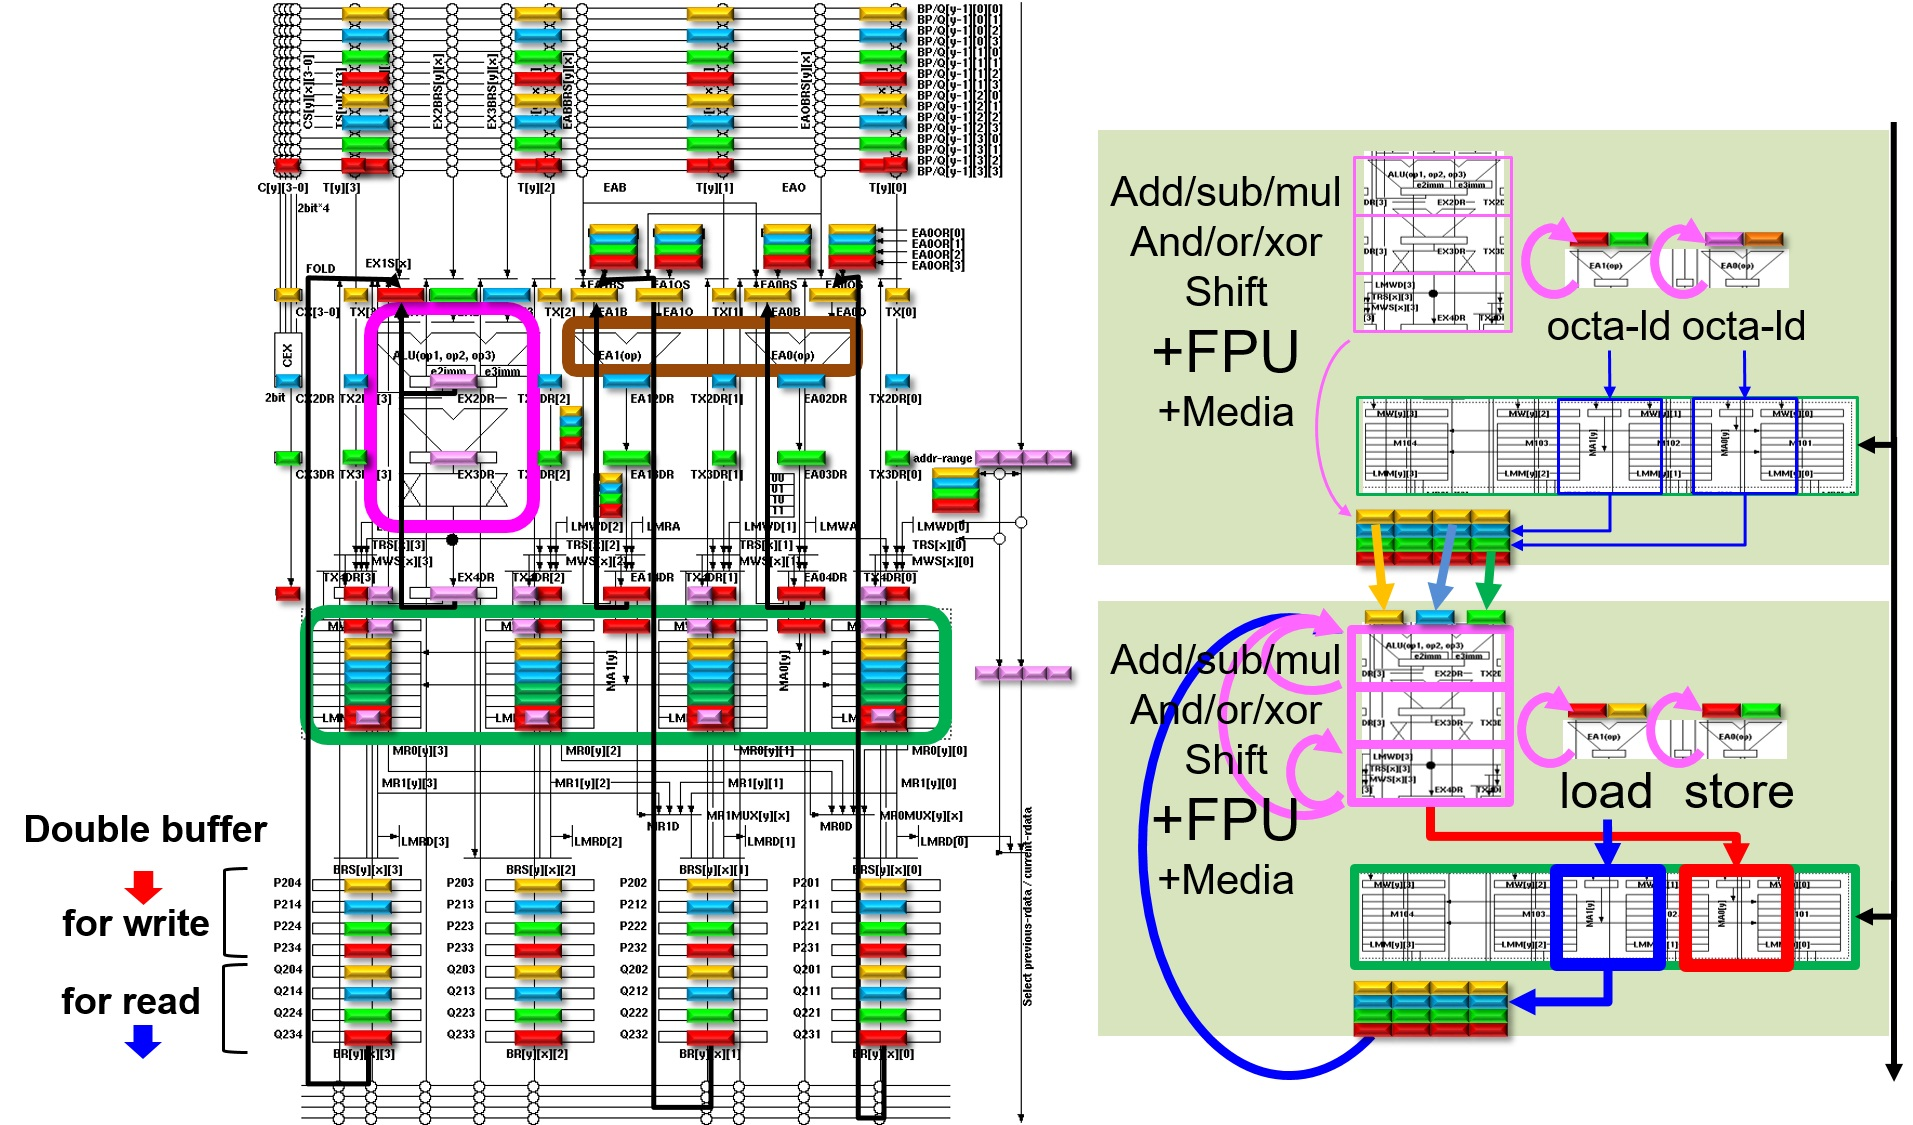
\includegraphics[angle=270,origin=b,width=0.98\textwidth]{IMAX1.eps}
\caption{\label{imax1}Basic structure of a unit}
\end{figure}

\begin{figure}[htbp]
\center
\epsfile{file=EMAX6EXE.eps,width=0.98\textwidth}
\caption{\label{exe}Configuration and timing of arithmetic in UNIT}
\end{figure}

\begin{figure}[htbp]
\center
\epsfile{file=EMAX6LMM.eps,width=0.98\textwidth}
\caption{\label{lmm}Configuration and timing of local memory (LMM) in UNIT}
\end{figure}

\begin{figure}[htbp]
\center
\epsfile{file=EMAX6PMM.eps,width=0.98\textwidth}
\caption{\label{pmm}direct reference of Local memory (LMM) from CPU}
\end{figure}

The arithmetic unit of each UNIT includes: integer arithmetic,
single-precision floating-point arithmetic, and multimedia arithmetic.
Figure \ref{exe} is a reference timing chart of registers specific for
arithmetic unit. The arithmetic functions for four columns are realized by
multiple execution using hardware for one column. Register reading and unit
calculation are divided into 4 pipelined cycles.  Figure \ref{lmm} is a
reference timing chart of registers specific for LMM. Similarly, the LMM
function for four rows is realized by multiple execution using hardware for
one row. The LMM is divided into up to four parts, and four references are
pipelined. If the LMM is not divided, the 18 bits output from EA0/1 are used
as it is for addressing the LMM. When the LMM is divided into four parts,
the upper 2 bits of the 18 bits output from EA0/1 are overwritten to one of
00/01/10/11 according to the column number and used to specify the address
of the LMM.  Figure \ref{pmm} shows the data path configuration of DMA/PIO
used when directly referencing LMM from CPU. In each cycle: address, R/W
type, and write data in case of writing are supplied from the previous row,
read memory is read out from the last row by referring to the memory space
composed of multiple rows in a pipeline manner. In which the UNIT's LMM
containing the destination address is determined by comparing the address
with the vAddr-range (top, len) in each UNIT. If the own LMM matches, the R
/ W operation is performed. The address and data are passed to the next
line. Even if they do not match, the address and data are passed to the next
line.

\clearpage

\begin{figure}[htbp]
\center
\epsfile{file=EMAX6MAP.eps,width=0.98\textwidth}
\caption{\label{emax6map}UNIT features}
\end{figure}

Figure \ref {emax6map} (a) to (j) are functions that can be mapped to UNIT.
In (a), LDRQ (4 dwords) / LDR (1 dword) supplies the loaded data to the
arithmetic unit on the next row while preloading the data from the main
memory required for the next execution into the LMM. For preload, blk (0: no
blocking, 1: Blocking that advances the leading pointer array every 16
consecutive references, 2: Blocking to advance the leading pointer array
every 32 consecutive references, 3: Blocking that advances the leading
pointer array for every 64 consecutive references, and len (burst length in
32-bit units) are specified.

(b) transfers the previous execution result to the main memory while storing
the operation result into the LMM by STRQ (4 dwords) / STR (1 dword). STRQ
stores 1dword per cycle to store logical multi-column operation results in
LMM. For this reason, it is not possible to map multiple STRQs and preloads
on the same line.

(c) performs LMM read-modify-write in the same UNIT. The range specified by
top, blk, and len is stored in LMM in advance. After that, the data read by
LDRQ is returned to the operation unit input, and the result is written back
to the same LMM. With the multi-threading function, the pipeline does not
stop even if such an accumulation is mapped.

(d) prior to LDR loading from LMM, the range specified by top, blk, and len
is stored in LMM in advance. After that, the LDR refers to the LMM based on
random addressing. LDRs with the same top, blk, and len are mapped to the
same unit using the dual port function of the LMM.

(e) is paired with (d), the calculation result is stored in LMM by
STR. After all stores are completed, the amount of data specified by len is
burst-transferred from the LMM to the main memory.

(f) is a transaction. The operation results are stored in the LMM by TR (4
dwords) and the 4 dwords required for the transaction are supplied to the
ARM. TR stores 1dword per cycle in order to store logical multi-column
operation results in LMM. For this reason, it is not possible to map
multiple TRs and preloads on the same line.

(g) is a function to load directly from external memory. The main memory
address calculation is mapped to EX, and the address is queued in dword0 of
LMM. EA0 is used for LMM writing, ARM monitors the AXRA (the same value as
EA0), detects the registration of a new address, extracts the main memory
address from LMM, reads the main memory using AXI, Send data to LMWD. In
UNIT, 4dword is sent to the next line via: LMWD to TR to BR.

By the way, among the above basic functions, in the mapping of (g), it is
necessary to consider the main memory delay. Although no special description
is required during programming, in the unit included in the same line as
(g), the delay synchronization mechanism using LMM is activated as in
(h). Similarly, when inter-register propagation is necessary, functions such
as (i) (without delay synchronization) and (j) (with delay synchronization)
are mapped using empty registers.

\section{Simulator}

For rapid and accurate prototype development, it is essential to develop a
detailed simulator that can be converted to Verilog on a one-to-one
basis. This is because the operation speed of the Verilog simulator is
extremely slow, making it difficult to verify the operation of large-scale
applications. In addition, for a hardware design verification using a
Verilog simulator, an accurate expected value for comparing with a correct
value of a register value is necessary. Since IMAX is controlled by ARMv8,
an IMAX simulator that can simulate ARMv8 has been developed (17K lines in C
language). Using the application program, IMAX compiler, and this simulator,
a test program with an expected value comparison function and a test bench
for Verilog simulation, which are essential for hardware debugging, were
prepared before starting the design of the prototype system.

\section{Multichip prototype on FPGA}

\begin{figure}[htbp]
\center
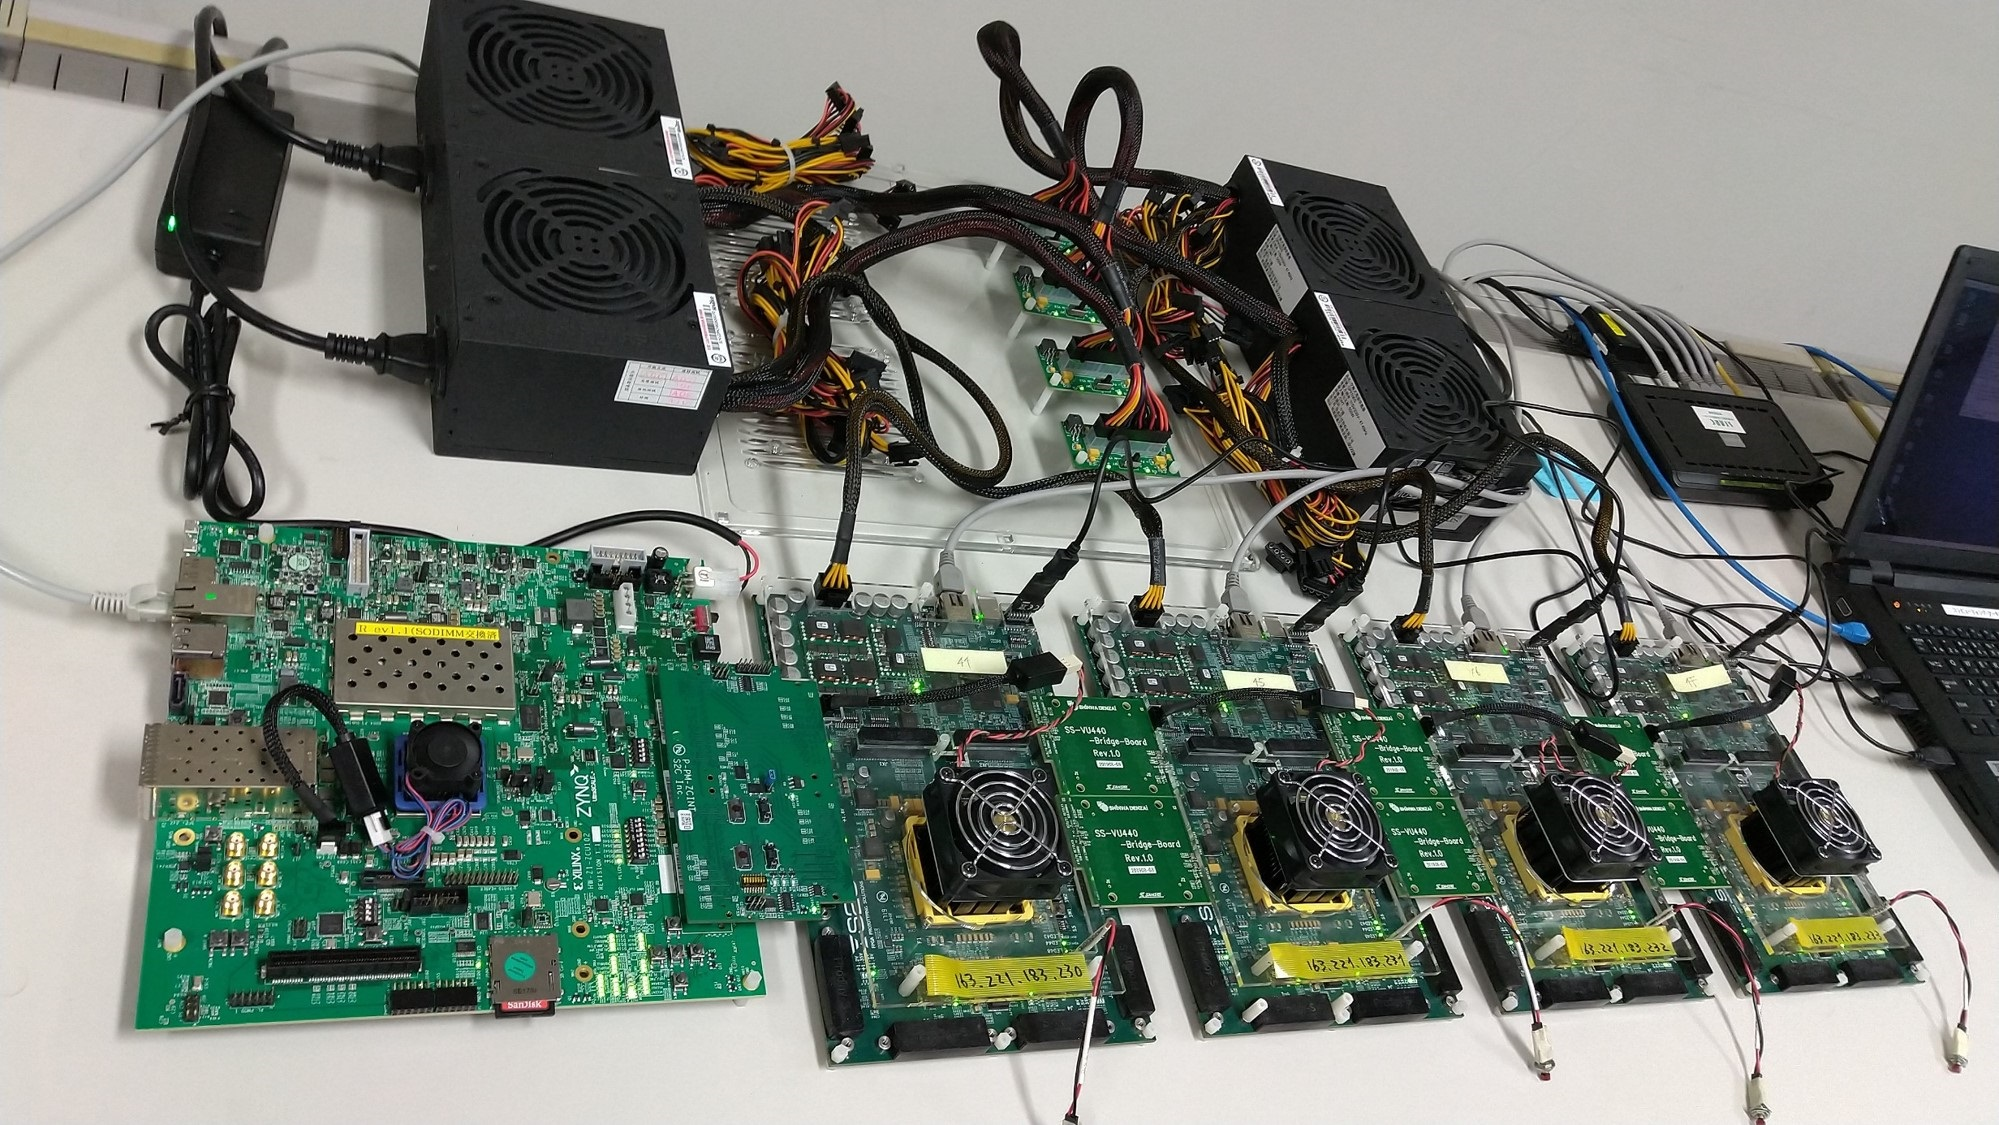
\includegraphics[angle=270,origin=b,width=0.98\textwidth]{IMAX4.eps}
\caption{\label{imax4}IMAX with 4-chip configuration}
\end{figure}

In order to evaluate the eight-chip configuration on a real machine, a test
environment with eight XILINX VU440s is required. Verilog description was
completed based on the simulator described above, and debugging was
performed by comparing the correct value of each register generated by the
simulator with the Verilog simulation result.  The amount of hardware
description was 11K lines in Verilog. HOST is Xilinx Zynq UltraScale +
(ZCU102) equipped with ARMv8 (industrial standard CPUs for edge
devices). For IMAX, Virtex Ultra Scale (S2C Single VU440 Prodigy Logic
Module) provided by and S2C company is used (Figure \ref{imax4}). Even
today, the only FPGA that can mount the IMAX with 64 units is VU440, and
this combination is optimal as a system that can connect ARMv8 and VU440 by
a high-speed serial link. However, according to the catalog specification,
three lanes of high-speed serial links of 10 Gbps could be bundled to
achieve a throughput of 30 Gbps, but in actuality, links could only be
established with a total of 5 Gbps x 3 lanes = 15 Gbps (later, increased to
8 lanes).  Also, when 8 chips were connected, the AXI-READ operation used
for reading data from the LMM was found to be extremely slow. The reason is
that: even if you specify a burst length long enough for the DMA function of
HOST, and AXI interface built in HOST is AXI3 compatible, In the case of
256-bit width transfer, the transfer was interrupted every 8 beats, and the
next AXI-READ must wait until the response from all chips was
completed. Therefore, we propose a method that do not break the transfer
between IMAX even though we still use the original burst length, and HOST��s
interface is still AXI3. The results have shown that speed of AXI-READ is
significantly improved.

\section{Comprehensive Evaluation}

\begin{figure}[htbp]
\center
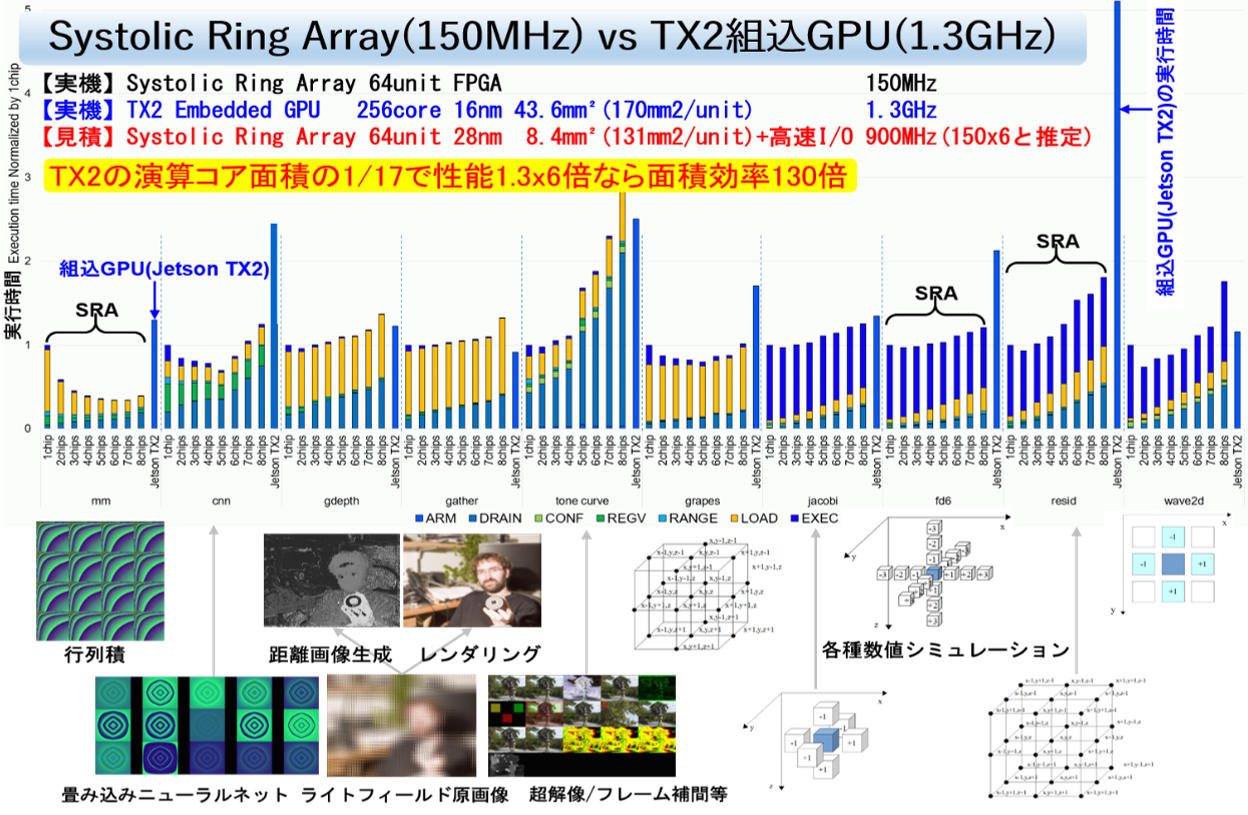
\includegraphics[angle=270,origin=b,width=0.98\textwidth]{result1.eps}
\caption{\label{result1}Comprehensive Evaluation 1 (15Gbps interface)}
\end{figure}

\begin{figure}[htbp]
\center
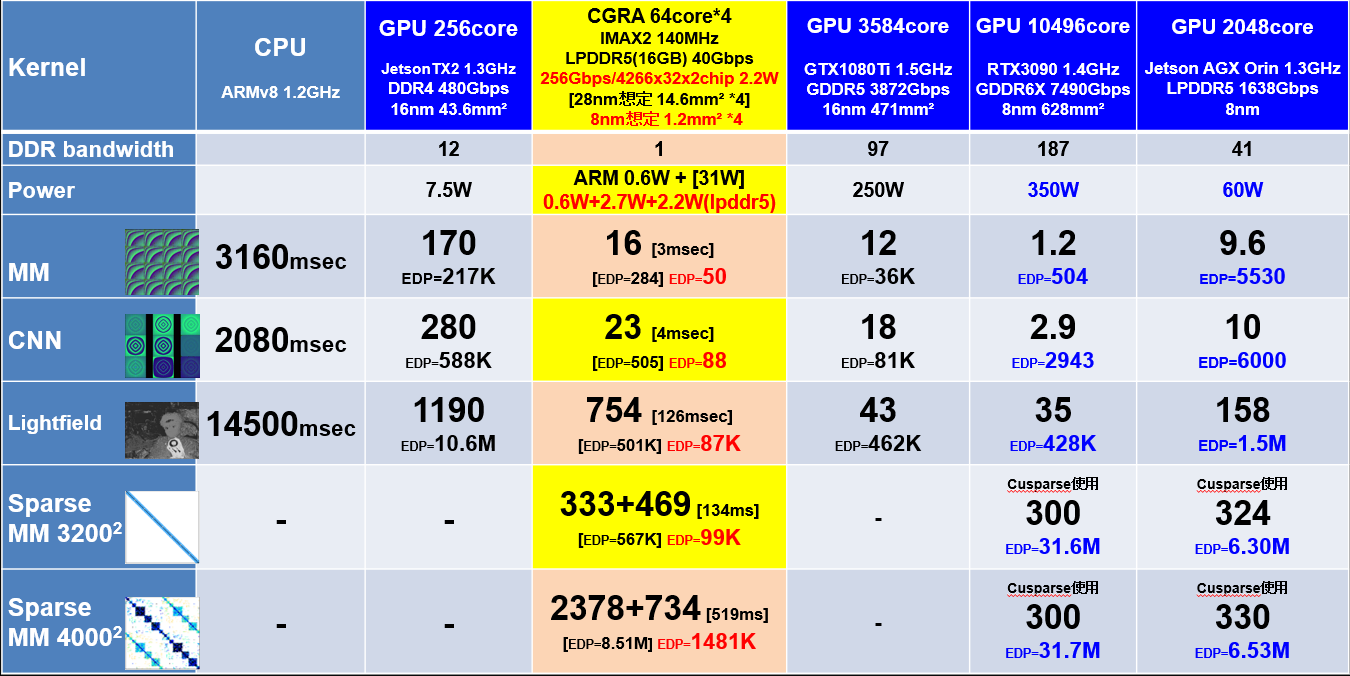
\includegraphics[angle=270,origin=b,width=0.98\textwidth]{result2.eps}
\caption{\label{result2}Comprehensive Evaluation 2 (40Gbps interface)}
\end{figure}

Various programs have been run using the IMAX 8-chip configuration model
that had been developed through the above processes. Figure \ref{result1}
shows the application execution time measured by changing the number of IMAX
chips from 1 to 8 using 15Gbps interface. Each program is normalized based
on the execution time of one chip configuration (operating frequency 150
MHz, number of arithmetic units 64, area 8.4 mm2 estimated at 28 nm).  For
comparison, the execution time of a built-in GPGPU (Jetson TX2: operating
frequency 1.3 GHz, number of arithmetic units 256, arithmetic core area 16
nm estimated at 43.6 mm2) is also shown.  Matrix multiplication (mm) uses 7
connected chips, convolution (cnn) uses 5 connected chips, and depth-extraction
(depth) uses 2 connected chips. For scientific and technical calculation
(Stencil calculation), the atmospheric simulation (grapes) uses 5 connected
chips. Other stencils were fastest with 2 connected chips.  As a general
trend, the effect of multichip formation is large when there is a lot of
common data between chips such as mm and cnn, and the effect is small with
simple space division such as stencil (it is not necessary to create a
multi-chip with a narrow memory bandwidth). In general, we have achieved
satisfied result within the limited memory bandwidth for Edge devices (1/32
of Jetson TX2).  Figure \ref{result2} shows the application execution time
using 40Gbps interface. The fact that the IMAX operating at 140MHz
outperforms the Jetson TX2 operating at 1.3GHz in terms of performance is a
sufficient indication of the potential of CGRAs. Also, if the IMAX operates
at 900MHz with 28nm ASIC, the performance is up to 70 times (in the case of
four chip cnn) with 1/2 of the area of Jetson TX2, and 140 times the
performance per area. If we consider that power consumption is proportional
to area, we can assume that power consumption per the same performance has
the same ratio.


\chapter{IMAX Software}

\section{IMAX interface mapped on CPU memory space}

\begin{figure}[htbp]
\center
\epsfile{file=EMAX6MMAP.eps,width=0.98\textwidth}
\caption{\label{mmap}Physical memory space}
\end{figure}

Figure \ref {mmap} shows the physical memory space of the CPU.  Physical
memory space related to IMAX includes: (1) FPDDMA-CH1 DMA control register
space that controls DMA between CPU physical memory space and LMM (DMA
control register space: 4KB), (2) The LMM DMA space (pAddr2 space: 2GB)
which maps the LMM to the CPU physical memory space and refers by DMA, the
control register space (pAddr2+ space: 2GB) which refers to the registers in
IMAX by PIO, (3) Consists of a DDR memory space (pAddr space: 2GB) that
connect DMA with LMM. Therefore, the space that can be referenced by
physical connection with IMAX is pAddr2 space: 2GB and pAddr2+ space: 2GB.
Since the total capacity of the LMM in the IMAX is 16MB (256KB * 64stages)
and the data bus width is 256bit (32B), at least 19bit is required for the
address width and 4bit is required for masking (1bit write mask for each
1dword (64bit)).  The physical memory space, which includes the control
register space, is mapped to the physical memory space of the CPU.

\begin{table}[htbp]
\center\footnotesize
\caption{\label{logicinterface}Logical interface}
\tabcolsep 0.2pc
\begin{tabular}{l|c|l|p{3.4in}}\hline\hline
����쥸��������(pAddr2+)	& R/W	& Bit����    & ���� \\\hline
STATUS				&	&	     & \\
0x400000007-0x400000000		& R	& bit3-0     & EXRING���� 0:IDLE, 1:BUSY(SCON/EXECư����) \\
				&  	& bit7-4     & LMRING���� 0:IDLE, 1:BUSY(PIO/DMAư����) \\
				&  	& bit11-8    & 0:EMAX\_DEPTH=8,  1:EMAX\_DEPTH=16 \\
				&  	&            & 2:EMAX\_DEPTH=32, 3:EMAX\_DEPTH=64 \\
				&  	& bit15-12   & 0:LMM\_SIZE=32KB, 1:LMM\_SIZE=64KB, 2:LMM\_SIZE=128KB \\
				&  	&            & 3:LMM\_SIZE=256KB, 4:LMM\_SIZE=512KB \\
				&       & bit63-16   & reserved by 0 \\\hline
COMMAND				&	&	     & IMAX�ؤλؼ� \\
0x400000017-0x400000010		& W	& bit1-0     & 0:NOP, 1:RESET, 2:SCON, 3:EXEC \\
				&       & bit31-2    & reserved by 0 \\
				&       & bit35-32   & chip�ֹ�(0��񤭹����chip�֤�缡����)\\
				&       & bit63-36   & reserved by 0 \\\hline
ADRTRANS			&	&	     & vAddr-pAddr2 \\
0x400000027-0x400000020		& W	& bit63-0    & DDR-LMM��DMA���Υ��ɥ쥹�Ѵ����� \\\hline
COLSELECT			&	&	     & vAddr-pAddr2 \\
0x400000037-0x400000030		& W	& bit1-0     & DMA/LDDMQ/TRANS��������Ū����col���� \\
				&       & bit63-2    & reserved by 0 \\\hline
CONF	  			& 	&            & \\
0x40000201f-0x400002000		& W 	& bit255-0   & ����UNIT\#0.0��conf \\
0x40000203f-0x400002020		& W 	& bit255-0   & ����UNIT\#0.1��conf \\
:                            	& :	&            & : \\
0x400003fff-0x400003fe0		& W 	& bit255-0   & ����UNIT\#63.3��conf \\\hline
REGV-BR				&	&            & BR�񤭹��� \\
0x40000401f-0x400004000		& W	& bit255-0   & ����UNIT\#0.0��BR[3:0] \\
0x40000403f-0x400004020		& W	& bit255-0   & ����UNIT\#0.1��BR[3:0] \\
:				& :	&            & : \\
0x400005fff-0x400005fe0		& W	& bit255-0   & ����UNIT\#63.3��BR[3:0] \\\hline
REGV-EAR/vAddr-range		&	&            & EAB,EAO�񤭹��� \\
				&	&            & LMM��Ƭaddr(max2GB),LMMͭ��dword��(max8KDW) \\
0x40000600f-0x400006000		& W	& bit50-32,18-0   & ����UNIT\#0.0��ea0o,ea0b(virt-addr)    \\
				&  	& bit114-96,82-64 & ����UNIT\#0.0��ea1o,ea1b(virt-addr)    \\
0x400006017-0x400006010		& W	& bit31-0    & ����UNIT\#0.0��top(virt-addr)    \\
				&  	& bit63-32   & ����UNIT\#0.0��bot(virt-addr)    \\
0x40000602f-0x400006020		& W	& bit50-32,18-0   & ����UNIT\#0.1��ea0o,ea0b(virt-addr)    \\
				&  	& bit114-96,82-64 & ����UNIT\#0.1��ea1o,ea1b(virt-addr)    \\
0x400006037-0x400006030		& W	& bit31-0    & ����UNIT\#0.1��top(virt-addr)    \\
				&  	& bit63-32   & ����UNIT\#0.1��bot(virt-addr)    \\
:				& :	&            & : \\
0x400007fef-0x400007fe0		& W	& bit50-32,18-0   & ����UNIT\#63.3��ea0o,ea0b(virt-addr)   \\
				&  	& bit114-96,82-64 & ����UNIT\#63.3��ea1o,ea1b(virt-addr)   \\
0x400007ff7-0x400007ff0		& W	& bit31-0    & ����UNIT\#63.3��top(virt-addr)   \\
				&  	& bit63-32   & ����UNIT\#63.3��bot(virt-addr)   \\\hline
LDDMQ/TRANS-R			&	&	     & LMM����LDDMQ/TRANS�׵���ɤ߽Ф� \\
0x40000801f-0x400008000		& R	& bit255-0   & ����UNIT\#0.0��LMM \\
0x40000803f-0x400008020		& R	& bit255-0   & ����UNIT\#0.1��LMM \\
:                            	& :	&            & : \\
0x400009fff-0x400009fe0		& R	& bit255-0   & ����UNIT\#63.3��LMM \\\hline
LDDMQ-W				&	&	     & TR�ؤν��ᤷ \\
0x40000801f-0x400008000		& W	& bit255-0   & ����UNIT\#0.0��TR \\
0x40000803f-0x400008020		& W	& bit255-0   & ����UNIT\#0.1��TR \\
:                            	& :	&            & : \\
0x400009fff-0x400009fe0		& W	& bit255-0   & ����UNIT\#63.3��TR \\\hline\hline
LMM����(pAddr2)			& R/W	& Addr����   & ���� \\\hline
0x4ffffffff-0x480000000		& R/W	& 32B        & DDR-High(0x87fffffff-0x800000000)���б����֤˳�������LMM�����Ƥ�R/W���롥\\\hline
\end{tabular}
\end{table}

Table \ref {logicinterface} shows the logical interface provided through the
physical memory interface. Within the physical memory space,
0x4ffffffff-0x480000000 (pAddr2) is a continuous physical space used by the
FPDDMA mechanism for DMA between DDR-High and LMM corresponding to
0x87fffffff-0x800000000 (pAddr).  The user program does not refer to the
continuous virtual space (vAddr2) obtained by the mmap () of the continuous
physical space (pAddr2) by PIO, but is obtained exclusively by the mmap ()
of the DDR-High continuous physical area (pAddr). Refers only to the
continuous virtual space (vAddr). Specifically, IMAX uses vAddr when
referencing LMM in conjunction with computation unit. In order to obtain the
same contents of the DDR-High address from the LMM, the CPU must transfer
the contents of vAddr to the LMM in advance.  The destination LMM is
specified by comparing it with the vAddr-range register provided for each
UNIT. As the write destination address, we use vAddr obtained by adding
pAddr2 (notified from FPDDMA to FSM) with the value of the address
conversion register in FSM (vAddr-pAddr2). The vAddr-range register provided
in each UNIT is associated with the latest logical UNIT number obtained by
subtracting the conf.mapdist value of each UNIT for each SCON
instruction. Therefore, when the LMM is ideally reused with instruction
shift, it corresponds to the newly enabled LMM. Only writing to the
vAddr-range register needs to be performed.

\begin{figure}[htbp]
\center
\epsfile{file=EMAX6PROC.eps,width=0.98\textwidth}
\caption{\label{proc}Procedure from start-up to termination}
\end{figure}

\begin{figure}[htbp]
\center
\epsfile{file=EMAX6LMRING.eps,width=0.98\textwidth}
\caption{\label{lmring}Relationship between logical interface and data capture mechanism in each line}
\end{figure}

Figure\ref{proc} is a comparison of the operation outline from start to
termination of EMAX5 and IMAX. In the case of EMAX5, CPU activates FSM in
EMAX via HPM, and FSM operates as AXI-MASTER until IDLE status is notified
to CPU.  In the case of IMAX, the CPU side becomes AXI-MASTER, and FSM
operates as AXI-SLAVE. The DMA-CHAIN function of FPDDMA is used for DRAIN
and LOAD, and PIO is used for CONF, SCON, REGV, RANGE, and EXEC.  The LMMI
placed in EMAX5 is managed by the CPU in case of IMAX, and transmission to
IMAX is not required, but a new update of vAddr-range (RANGE) is required.
Using Fig.\ref{lmring}, the hardware operation in each procedure shown in
Fig. \ref {proc} is explained. Note that CONF, SCON, REGV, and RANGE can
only operate independently, while EXEC and DMA can operate simultaneously
(DMA is started immediately after EXEC is started).

\begin{description}
\itemsep 0in
\parskip 0in
\item[RESET] The CPU initializes the IMAX internal state by writing RESET
to COMMAND, and initializes the writing to the physical stage \# (fixed
value) in logical stage \# for all units. This function is for debugging
during IMAX development, and does not need to be used by user programs. When
IMAX is in RESET operation, BUSY is displayed in STATUS.EXRING.

\item[CONF] CPU can update CONF continuously by PIO when STATUS.EXRING and
STATUS.LMRING are IDLE. The CONF is assigned a physical address
corresponding to the logical UNIT number. By writing to the specified
physical address, the CONF of the logical UNIT having the logical stage \#
corresponding to the logical row number (bits 12-7 of pAddr2 +) is
updated. If IMAX is writing CONF, BUSY is displayed in STATUS.LMRING.

\item[SCON] By writing SCON to COMMAND when STATUS.EXRING is IDLE, CPU can
instruct all lines to start shifting CONF according to the value of
conf.mapdist stored in each line. For all rows, in the first cycle, the
first 256 bits of the own CONF information (256 bits * 4set) are written to
BR, and in the second cycle, the CONF information of all the rows from the
BR in the previous row is imported to the own row. By repeating the above
four times, all CONF information is shifted down by one line. Also, decrease
the value of logical stage \# by one. By repeating the above process
conf.mapdist times, all CONF information is shifted by conf.mapdist lines,
and the value of logical stage \# is reduced by conf.mapdist. The contents
of REGV are destroyed by SCON. When IMAX is in SCON operation, BUSY is
displayed in STATUS.EXRING.

\item[REGV] CPU can update REGV-EAR and REGV-BR continuously by PIO when
STATUS.EXRING and STATUS.LMRING are IDLE. The REGV is assigned a physical
address corresponding to the logical UNIT number. By writing to the
specified physical address, the REGV of the logical UNIT having the logical
stage \# that matches the logical line number (bits 12-7 of pAddr2 +) is
updated. When IMAX is writing REGV, then BUSY is displayed in STATUS.LMRING.

\item[RANGE] The CPU can continuously update vAddr-range by PIO when
STATUS.EXRING and STATUS.LMRING are IDLE. In the vAddr-range, a physical
address is assigned corresponding to the logical UNIT number, and by writing
to the specified physical address, a logical having a logical stage \#
corresponding to the logical line number (bits 12-7 of pAddr2 +) UNIT
vAddr-range is updated. The instruction (conf.lmm \_mode) to specify the LMM
as invalid, no division, two divisions, or four divisions is included in the
above CONF. If IMAX is writing vAddr-range, then BUSY is displayed in
STATUS.LMRING.

\item[DMA] When STATUS.LMRING is IDLE, the CPU can start continuous DDR-LMM
transfer by DMA. In EMAX5, the function realized by fsm is performed by the
CPU in DMA in IMAX. Specifically, the old lmmi must be compared with the new
lmmi, and when the old lmmi is the write destination (lmw), or when the old
lmmi is a target for forced LOAD+STORE (lmx), the DMA must be started to
expel the LMM to main memory.  If the area corresponding to the new lmmi
does not exist in the LMM, or if it is a target for forced LOAD (lmf or
lmx), the DMA from the main memory to the LMM must be started. If IMAX is in
DMA operation, then BUSY is displayed in STATUS.LMRING.

\item[EXEC] When STATUS.EXRING is IDLE, the CPU can instruct EXEC to start
execution for all lines by writing EXEC to COMMAND. When IMAX is in EXEC
operation, BUSY is displayed in STATUS.EXRING.

\item[LDDMQ] During EXEC operation, in the logical UNIT to which OP \_LDDMQ
is mapped, the main memory reference request is queued in the LMM. The
queuing state is notified to fsm, and fsm reads a reference request
(starting virtual address) from the LMM. At this time, fsm identifies the
target logical UNIT by setting the logical row number in bits 12-7 of imax
\_rw = 0, imax \_ty = 1, imax \_a [31: 5]. The read data is stored in the
buffer inside fsm and prepares for reading from CPU.  CPU should issue a
read request for a specific register space at appropriate intervals. When
LDDMQ request is queued in the LMM, the requests are output using a set of
\textbf{avo}, \textbf{sqo}, and \textbf{do}.  After acquiring the virtual
address, the CPU must refer to DDR-High and write to the TR of that UNIT.

\item[TRANS] During EXEC operation, in a logical UNIT to which OP \_TR is
mapped, a main memory reference request is queued in the LMM. The queuing
state is notified to fsm, and fsm reads a TRANS request from the LMM. At
this time, fsm specifies the target logical unit by setting the logical line
number in bits 12-7 of imax \_rw = 0, imax \_ty = 2, and imax \_a [31:
5]. The read data is stored in the buffer inside fsm and prepares for
reading from CPU. CPU should issue a read request for a specific register
space at appropriate intervals. When TRANS requests are queued in the LMM,
the requests are output using a set of \textbf{avo}, \textbf{sqo}, and
\textbf{do}.  The CPU must execute the Transaction after acquiring the TRANS
request.
\end{description}

\section{Control Registers}

Figure \ref {reg_ctrl} shows the detailed structure of the control
registers.  Figure \ref {conf} shows the detailed structure of the registers
in units set by CONF.

\begin{figure}[htbp]
\center
\begin{screen}
\footnotesize
\begin{verbatim}
struct reg_ctrl {
 struct i0 {
  Ull  stat; /* +0000 bit15-12:LMM_SIZE, bit11-8:EMAX_DEPTH, bit7-4:LMRING, bit3-0:EXRING */
  Uint mcid; /* +0008 maximum chip-ID of IMAX (<EMAX_NCHIP) to be chained (activated) */
  Uint dmy0;
  Uint cmd;  /* +0010 host writes Ull cmd then chip# is propagated to succesors */
/*Uint cid;*//* +0012 chip# ( set by write to cmd ) */
  Uint dmy1;
  Ull  dmy2;
  Ull  adtr; /* +0020 */
  Ull  dmy3;
  Ull  csel; /* +0030 */
  Ull  dmrp; /* +0038 DMAREAD-PREF */
  Ull  dmy4[1016];
  struct conf                    conf[AMAP_DEPTH][EMAX_WIDTH];  /* +2000-3fff */
  struct {Ull  br[UNIT_WIDTH];}  breg[AMAP_DEPTH][EMAX_WIDTH];  /* +4000-5fff */
  struct {
    Uint ea0b ; /* ea0 base   (for avoiding ld-mask-st, */
  /*Ull  dmy0 :14;*/        /* should be extended to 32bits (lower 18bit is available)) */
    Uint ea0o ; /* ea0 offset (for avoiding ld-mask-st, */
  /*Ull  dmy1 :14;*/        /* should be extended to 32bits (lower 18bit is available)) */
    Uint ea1b ; /* ea1 base   (for avoiding ld-mask-st, */
  /*Ull  dmy2 :14;*/        /* should be extended to 32bits (lower 18bit is available)) */
    Uint ea1o ; /* ea1 offset (for avoiding ld-mask-st, */
  /*Ull  dmy3 :14;*/        /* should be extended to 32bits (lower 18bit is available)) */
    Uint top  ; /* LMM-top virtual-address */
  /*Ull  dmy4 : 1;*/
    Uint bot  ; /* LMM-bot virtual-address */
  /*Ull  dmy5 : 1;*/
    Ull  dmy6 ;}           addr[AMAP_DEPTH][EMAX_WIDTH];       /* +6000-7fff */
  struct {Ull reg[UNIT_WIDTH];} lddmrw[AMAP_DEPTH][EMAX_WIDTH];/* +8000-9fff *//*lddmq/trans-r,lddmq-w*/
  Ull dmy5[3072]; /* +a000-ffff */
 } i[EMAX_NCHIP]; /* 0000-ffff */
};
\end{verbatim}
\end{screen}
\caption{\label{reg_ctrl}Control Registers}
\end{figure}

\clearpage

\begin{figure}[htbp]
\center
\begin{screen}
\footnotesize
\begin{verbatim}
struct conf { /* final configuration info. for IMAX-CGRA */
  struct cdw0 { /* select EXE-in */
    Ull  v      :  1; /* 0:inv, 1:insn mapped */
    Ull  op1    :  6; /* alu_opcd */
    Ull  op2    :  3; /* logical_opcd */
    Ull  op3    :  3; /* sft_opcd */
    Ull  ex1brs :  4; /* 0:br0_0, 1:br0_1, ... 15:3_3 */
    Ull  ex1s   :  1; /* 0:ex1brs, 1:exdr(self-loop) */
    Ull  ex1exp :  3; /* 0:H3210, 1:H1010, 2:H3232, 3:B5410, 4:B7632 */
    Ull  ex2brs :  4; /* 0:br0_0, 1:br0_1, ... 15:3_3 */
    Ull  ex2exp :  3; /* 0:H3210, 1:H1010, 2:H3232, 3:B5410, 4:B7632 */
    Ull  ex3brs :  4; /* 0:br0_0, 1:br0_1, ... 15:3_3 */
    Ull  ex3exp :  3; /* 0:H3210, 1:H1010, 2:H3232, 3:B5410, 4:B7632 */
    Ull  e2is   :  2; /* 0:e2imm, 1:ex2, 2:ex3 */
#define E3IMMBITS  6
    Ull  e3imm  : E3IMMBITS;
    Ull  e3is   :  1; /* 0:e3imm, 1:ex3 */
    Ull  init   :  2; /* bit0:activate s1+INIT0 bit1:activate s2+INIT0 */
    Ull  fold   :  1; /* 0:normal, 1:load-exe-store folding */
    Ull  mex0op :  2; /* mex(sparse matrix) conditional 0:NOP, 1:AL, 2:OP_CMPA_LE, 3:GE */
    Ull  mex0init: 1; /* mex(sparse matrix) 0:none, 1:INIT0? */
    Ull  mex0dist: 3; /* distance 0:0, 1:1, 2:2, 3:4, 4:8, 5:16, 6:32, 7:64byte */
    Ull  mex1op :  2; /* mex(sparse matrix) conditional 0:NOP, 1:AL, 2:OP_CMPA_LE, 3:GE */
    Ull  mex1init: 1; /* mex(sparse matrix) 0:none, 1:INIT0? */
    Ull  mex1dist: 3; /* distance 0:0, 1:1, 2:2, 3:4, 4:8, 5:16, 6:32, 7:64byte */
    Ull  mexlimit: 4; /* limit 0:0, 1:8, 2:16, .... 11:8192, 12:16384, 13:32768 14:65536, 15:131072 */
    Ull  dmy00  :  1;
  } cdw0;
  struct cdw1 { /* select CEX-in and EAG-in */
    Ull  cs0    :  4; /* 0:br0_0, 1:br0_1, ... 15:3_3 */
    Ull  cs1    :  4; /* 0:br0_0, 1:br0_1, ... 15:3_3 */
    Ull  cs2    :  4; /* 0:br0_0, 1:br0_1, ... 15:3_3 */
    Ull  cs3    :  4; /* 0:br0_0, 1:br0_1, ... 15:3_3 */
    Ull  cex_tab: 16; /* c3.c2.c1.c0���ȹ礻 (cop=NOP�ξ��,ffff) */
                      /* 1111,1110,1101,1100,....,0001,0000 �γơ���0/1�������Ƥ�16bit����� */
    Ull  ea0op  :  5; /* mem_opcd */
    Ull  ea0bs  :  2; /* 0:ea0br, 1:ea0dr(ea0br+self-loop), 2:eabbrs, 3:ea0dr(eabbrs+self-loop) */
    Ull  ea0os  :  1; /* 0:ea0or, 1:eaobrs */
    Ull  ea0msk :  4; /* 14:64bit, 13:word1, 12:word0, 11-8:half3-0, 7-0:byte7-0 of offset */
    Ull  ea1op  :  5; /* mem_opcd */
    Ull  ea1bs  :  2; /* 0:ea1br, 1:ea1dr(ea1br+self-loop), 2:eabbrs, 3:ea1dr(self-loop) */
    Ull  ea1os  :  1; /* 0:ea1or, 1:eaobrs */
    Ull  ea1msk :  4; /* 14:64bit, 13:word1, 12:word0, 11-8:half3-0, 7-0:byte7-0 of offset */
    Ull  eabbrs :  4; /* 0:br0_0, 1:br0_1, ... 15:3_3 */
    Ull  eaobrs :  4; /* 0:br0_0, 1:br0_1, ... 15:3_3 */
  } cdw1;
  struct cdw2 { /* select TR/BR-in */
    Ull  ts0    :  4; /* 0:br0_0, 1:br0_1, ... 15:br3_3 */
    Ull  ts1    :  4; /* 0:br0_0, 1:br0_1, ... 15:br3_3 */
    Ull  ts2    :  4; /* 0:br0_0, 1:br0_1, ... 15:br3_3 */
    Ull  ts3    :  4; /* 0:br0_0, 1:br0_1, ... 15:br3_3 */
    Ull  trs0   :  2; /* 0:lmwd0, 1:exdr, 2:ts0 *//* 0:TR�����񤭹�����, 1,2:EX/TS�񤭹����� */
    Ull  trs1   :  2; /* 0:lmwd1, 1:exdr, 2:ts1 */
    Ull  trs2   :  2; /* 0:lmwd2. 1:exdr, 2:ts2 */
    Ull  trs3   :  2; /* 0:lmwd3, 1:exdr, 2:ts3 */
    Ull  mwsa   :  1; /* 0:lmwa,  1:ea0d        *//* 0:���lmwd��ǽ, 1,2:EXEC���ʳ��϶���lmwd��ǽ */
    Ull  mws0   :  2; /* 0:lmwd0, 1:exdr, 2:ts0 *//* 0:���lmwd��ǽ, 1,2:EXEC���ʳ��϶���lmwd��ǽ */
    Ull  mws1   :  2; /* 0:lmwd1, 1:exdr, 2:ts1 */
    Ull  mws2   :  2; /* 0:lmwd2, 1:exdr, 2:ts2 */
    Ull  mws3   :  2; /* 0:lmwd3, 1:exdr, 2:ts3 */
    Ull  brs0   :  2; /* 0:off, 1:mr10, 2:tr0, 3:mr0  */
    Ull  brs1   :  2; /* 0:off, 1:mr11, 2:tr1, 3:mr1  */
    Ull  brs2   :  2; /* 0:off, 1:mr12, 2:tr2, 3:exdr */
    Ull  brs3   :  2; /* 0:off, 1:mr13, 2:tr3         */
    Ull  mapdist:  6; /* ����UNIT��ˤ��뤬,�����ʪ��UNIT��1�ĤǤ褤 */
    Ull  lmm_mode: 2; /* ����LMM��˥��å� 0:̵��, 1:ʬ��̵, 2:2ʬ��, 3:4ʬ�� */
    Ull  lmm_axiw: 1; /* AXI->LMM write�о�(lmp/lmr/lmf/lmx�ξ��1) */
    Ull  lmm_axir: 1; /* AXI<-LMM read �о�(lmd/lmw/lmx    �ξ��1) */
    Ull  dmy20  : 13;
  } cdw2;
  struct cdw3 { /* e2 immediate */
    Ull  e2imm  : 64;
  } cdw3;
} conf[EMAX_DEPTH][EMAX_WIDTH]; /* 4dwords/unit costs 1cycle/unit: 4-parallel conf costs 1cycle/stage */
\end{verbatim}
\end{screen}
\caption{\label{conf}Configuration Registers}
\end{figure}

\clearpage

\section{Programming model}

\begin{figure}[htbp]
\center
\epsfile{file=IMAXMODEL.eps,width=0.98\textwidth}
\caption{\label{imaxmodel}Programming model of IMAX based on load-exec-store}
\end{figure}

It is common to employ compiler optimization to optimize a program for which
the algorithm has been determined. However, in the case of von Neumann
computers, the ultimate method for achieving high efficiency is still
programming in assembly language. Since machine language instructions are
executed logically in sequential, debugging is relatively easy with moderate
knowledge. Similarly, CGRA aims to improve efficiency by mapping machine
instruction level functions to a large number of arithmetic units at high
density. However, in the conventional CGRA in which arithmetic units are
interconnected in a mesh shape, it is difficult to accurately express the
operation by a sequential execution model such as the Neumann type, and it
is extremely difficult to optimize and debug at the assembly language level. 
In addition, since the arithmetic unit group and the external memory are
separated, a wide memory bus and SIMD operations are required. In order to
improve the above points, IMAX uses a pair of arithmetic unit and memory as
a basic component, and adopts a ring connection instead of a mesh connection
for the network between arithmetic units. Therefore, it is not restricted by
the SIMD operations and has a high degree of freedom regarding the mapping
position of load-exec-store. The programming procedure is first
load-exec-store dataflow description, then selection of appropriate local
memory location and mapping of addresses, and finally tuning for maximum
reuse of local memory.

Figure\ref{imaxmodel} shows a typical IMAX programming model. One logical
UNIT (colored by light blue) has an ALU, two address generators (EAG), and
dual port local memory, and four logical UNITs make up one row and four
columns of CGRA. Each line of source code can also contain position
information. The compiler selects one of the mapping patterns (a)-(d)
depending on the presence or absence of position information and the data
dependency, and maps it to an appropriate logical UNIT. (a) is a simple case
where "D = C + B * A" is calculated by using dual SIMD on arrays A, B, C,
and D without describing the position information. First, load A, load B,
and load C are mapped to the first row of CGRA (the fourth column is
omitted). In the second row, fused multiplication and addition (FMA) and
Store D are mapped (third and fourth columns are omitted). If no position
information is described, a simple data flow from top to bottom is formed
like this way.

On the other hand, (b) is a case where "D = C + B * A" is calculated on
arrays A, B, and C, and the result is written back to C. Position
information is attached to the register C for load destination and register
D for FMA destination, and the load and store to the array C are performed
at the same time. Load A and load B are mapped on the first row of CGRA, and
load C is mapped on the second row. When the temporal destination D of FMA
operation is specified on the same row as register C, the inputs A, B, and C
for the arithmetic unit are once sent to the bottom registers of the current
row and then forwarded to the input of ALU. Since register D for storing to
array C is also mapped to the same row, it becomes load-exec-store for array
C in the same local memory.

(c) is a case where (b) is integrated in one row. Physically, only one
dual-port local memory is located in one row of CGRA, and it looks like a
four logical memory structure by time-domain multiplexing. Therefore, in
(b), one physical local memory is shared by arrays A and B, whereas in (c),
array C is also shared, so the available memory space per array
decreases. If there is still a merit of integrating in one row, the position
information is not attached to the destination register C, but the position
information is attached only to the destination register D of FMA. First,
load A, load B, and load C are mapped, and the FMA operation and store D
operation for the array C are also mapped to the same row.

(d) is a case where the FMA operation is described as "C = C + B * A" without
using the temporary register D. No position information is attached to store
C. On the source code, it is a repetition of the FMA operation that reloads
the data stored in the local memory. However, the calculation that loads
data from the same address after the previous store completes has a large
overhead, and such kind of hardware operation should be avoided even by the
CPU. On the other hand, in the case of CGRA, this operation can be easily
absorbed by the accumulation in the arithmetic unit. The difference from (c)
is that the FMA is not a simple load-exec-store, but the input C0 is the
load result of the array C only for the first time of loop, and the result
of the first FMA is connected to the next load-exec-store operation. Of
course, in the case of a pipelined floating point arithmetic unit, the
accumulation in the arithmetic unit cannot be executed every cycle. As
mentioned above, IMAX has the advantage of not causing overhead in the
operation of logical UNIT even if there is an accumulation due to 4-column
multithreading, so (d) can be used without fear of performance degradation.

\section{Templates of instructions}

\leftline{\shabox{\bf
cex(OP\_CEXE, \&ex0-9, c3, c2, c1, c0, 16bit-pattern)
}}

\vskip .1in

The c3, c2, c2, and c1 are 64bit values respectively. The each of 4bit
result of the concatenation of four bit32 values and the concatenation of
four bit0 values becomes an bit position of 16bit-pattern.  Each of bit1 and
bit0 of ex[0-9] are set to the bit value extracted from the 16bit-pattern.
The bit1 and the bit0 of ex[0-9] correspond to the upper 32 bits and the
lower 32 bits of the conditional store.

\vskip .1in

\leftline{\shabox{\bf
\leftline{exe(OP\_X, \&var$|$\&AR[0-63][0-3], s1, e1, s2, e2, s3, e3, OP\_Y, s4, OP\_Z, s5)}
\leftline{ex4(OP\_X, \&var$|$\&AR[0-63], s1, e1, s2, e2, s3, e3, OP\_Y, s4, OP\_Z, s5)}
}}

\vskip .1in

Var or AR[0-63][0-3] is the destination of ALU, the former corresponds to no
position information, and the latter corresponds to the position
information. Each of 64-bit value of s1, s2 and s3 is sent to the ALU after
modification by e1, e2 and e3 respectively. The modifiers are as follows.

\begin{description}
\itemsep 0in
\parskip 0in
\item[EXP\_H3210:] no modification
\item[EXP\_H1010:] lower 32bit is copied to upper/lower 32bit
\item[EXP\_H3232:] upper 32bit is copied to upper/lower 32bit
\item[EXP\_B5410:] byte5,4,1,0 is zero-extented to 16bit and concatenated
\item[EXP\_B7632:] byte7,6,3,2 is zero-extented to 16bit and concatenated
\end{description}
OP\_X, OP\_Y and OP\_Z cover arithmetic operations, logical operations and
shift operations respectively. Each operation has dual SIMD mode where the
upper 32bit and lower 32bit are managed independently. exe() is dual SIMD,
and ex4() is octal SIMD.

\vskip .1in

\leftline{\shabox{\bf
exe(OP\_X, \&var, INIT0?var:var, e1, s2, e2, s3, e3, OP\_Y, s4, OP\_Z, s5)
}}

\vskip .1in

"INIT0?var:var" is redundant in the meaning of C language because it is
always "var". This expression is used by CGRA compiler as a hint to deal
with multiple loops in CGRA without host intervention.  Before starting the
multiple loop, the host sets each initial value for the inner loop in the
CGRA. Normally, when the inner loop is completed, the host needs to
intervene to reinitialize the internal registers. However, in IMAX, the
variable in which "INIT0?var:var" is described can be reinitialized by CGRA
using the initial values, and can successfully eliminate the overhead of
host intervention. Specifically, assuming that the initial value is set in
var, the initial value set in advance by the host is used as the first input
of the ALU for the first time (INIT0=1) of LOOP0, and the operation can be
continued by switching the input to the output of ALU.

\vskip .1in

\leftline{\shabox{\bf
exe(OP\_X, \&var, var, e1, INIT0?s2:0, e2, s3, e3, OP\_Y, s4, OP\_Z, s5)
}}

\vskip .1in

This is also a hint to deal with multiple loops in CGRA without host
intervention. When "INIT0?S2:0" is described, the data path is switched so
that s2 is the second input of the ALU for the first time (INIT0=1) of
LOOP0, and 0 is the second input from the next iteration. It can be used to
calculate the start address of a 2D subarray.

\vskip .1in

\leftline{\shabox{\bf
mex(OP\_MEX2, \&s2, INIT0?s20:s2, INIT0?0:expr, OP\_MEX1, \&s1, INIT0?s10:s1, INIT0?0:expr, limit, BR[0-63][0-3][1], BR[0-63][0-3][0])
}}

\vskip .1in

This is an address calculation auxiliary description for performing
multiple-loop sparse matrix calculation and merge sort without host intervention.
"INIT0?s20:s2" and "INIT0?s10:s1" correspond to the base address, and "INIT0?0:expr"
corresponds to the offset for increment. For the first time (INIT0=1) of
LOOP0, s20 and s10 (initial values) are stored in s2 and s1 respectively.
From the next iteration, the upper 32 bit of the two 64bit data read from the local memory last time are compared,
and s2 and s1, that are the output of EAGs, are added with 0 or expr depending on the comparison. 
And limit is the distance for merge sort. Refer to the sample program for detail. OP\_MEX is as follows.
\begin{description}
\itemsep 0in
\parskip 0in
\item[OP\_NOP:]      always base is used
\item[OP\_ALWAYS:]   always base+offset is used
\item[OP\_CMPA\_LE:] if upper 32bit (BR[][][1]) $\le$ upper 32bit (BR[][][0]) then base+offset, else base is used
\item[OP\_CMPA\_GE:] if upper 32bit (BR[][][1]) $\ge$ upper 32bit (BR[][][0]) then base+offset, else base is used
\end{description}

\vskip .1in

\leftline{\shabox{\bf
\leftline{mop(OP\_X, ex9-0, \&src$|$\&dst, base, offset, mask, top, len, block, force, ptop, plen)}
\leftline{mo4(OP\_X, ex9-0, \&src$|$\&dst, base, offset, mask, top, len, block, force, ptop, plen)}
}}

\vskip .1in

Description of load or store operations for local memory. Each field is as follows.
\begin {description}
\itemsep 0in
\parskip 0in
\item[OP\_X:] dual SIMD load or store operation according to the data width, mo4 is for octal SIMD
\item[ex0-9:] constant "3" for unconditional store, variable for conditional store
\item[src$|$dst:] destination register for load, source source register for store
\item[base:] the base part of the memory address "base + mask (offset)", the
host memory address can be used as it is, no need to be aware of address
translation because the address in local memory is automatically translated
by the cooperation of the compiler and hardware
\item[offset:] the offset part, note that the unit of offset is 1 byte
\item[mask:] the final address is base plus the value of the offset register
modified by mask, the mask is as follows
\begin{description}
\itemsep 0in
\parskip 0in
\item[MSK\_B0:] 64bit zero-extension of bit7-0
\item[MSK\_B1:] 64bit zero-extension of bit15-8
\item[MSK\_B2:] 64bit zero-extension of bit23-16
\item[MSK\_B3:] 64bit zero-extension of bit31-24
\item[MSK\_B4:] 64bit zero-extension of bit39-32
\item[MSK\_B5:] 64bit zero-extension of bit47-40
\item[MSK\_B6:] 64bit zero-extension of bit55-48
\item[MSK\_B7:] 64bit zero-extension of bit63-56
\item[MSK\_H0:] 64bit zero-extension of bit15-0
\item[MSK\_H1:] 64bit zero-extension of bit31-16
\item[MSK\_H2:] 64bit zero-extension of bit47-32
\item[MSK\_H3:] 64bit zero-extension of bit63-48
\item[MSK\_W0:] 64bit zero-extension of bit31-0
\item[MSK\_W1:] 64bit zero-extension of bit63-32
\item[MSK\_D0:] bit63-0 as it is
\end{description}
\item[top:] the start address of the host main memory for burst operation,
in which host DMA controller transmit data to/from LMM
\item[len:] the length of the burst operation, the unit is 1 word (4 bytes)
and the rate is 256 bits per cycle.  If constant(0) is specified, DMA is
supressed.  This case is used for double buffering in the same LMM.
\item[block:] not used in IMAX (only for DMA gather parameter in EMAX5)
\item[force:] different behavior in load or store operation as follows
\begin {description}
\itemsep 0in
\parskip 0in
\item[0:] In the case of load, if the start address and length of DMA last
time are the same, DMA is not started and LMM is reused. In the case of
store, data is transferred from the LMM to the host main memory after the
burst operation. However, if the delayed drain (with the next burst
operation) is specified, DMA is suppressed.
\item[1:] In the case of load, DMA from the host main memory to LMM is
always invoked.  Typical case is when the contents are different even if the
address is the same, such as the input of an external device. In the case of
store, the dirty-LMM is written back to the host main mamory first, and new
data is transferred in advance from the host main memory to LMM before the
burst operationn.
\end{description}
\item[ptop:] start address of overlapped DMA performed during burst
operation. In the case of load, the input required for the next burst
operation is transferred from the host main memory to LMM during the burst
operation (prefetch). In the case of store, the result of the previous burst
operation is transferred from LMM to the host main memory during the burst
operation (delayed drain). When mapdist=0, load / store and prefetch / drain
are performed on the same LMM.
\item[plen:] length of overlapped DMA. The unit is 1 word (4 bytes).
\end{description}

\clearpage

\section{List of instructions}

\begin{table}[htbp]
\center
\footnotesize
\caption{\label{lmm-operation}Memory operations}
\tabcolsep 0.2pc
\begin{tabular}{l|ll|p{0.9in}|p{1.1in}}\hline\hline
unit    & usage  &                                                                                & mode                & description\\\hline
MEX     & \multicolumn{2}{l|}{\_ALWAYS/CMPA\_LE/\_GE (\&base, INIT0?init:base, INIT0?0:[0-64], s2, s1)}  & sparse matrix& LMM indexed-access\\\hline
LD      & LDR    & (-,      (Ull*)d, base(++), offs, msk, top, len, blk, force-read, ptop, plen)  & 64bit      lmm      & LMM rand-access\\
        & LDWR   & (-,      (Ull*)d, base(++), offs, msk, top, len, blk, force-read, ptop, plen)  & u32bit     lmm      & LMM rand-access\\
%%      & LDHR   & (-,      (Ull*)d, base(++), offs, msk, top, len, blk, force-read, ptop, plen)  & u16bit     lmm      & LMM rand-access\\
        & LDBR   & (-,      (Ull*)d, base(++), offs, msk, top, len, blk, force-read, ptop, plen)  & u8bit      lmm      & LMM rand-access\\\cline{2-5}
        & LDRQ   & (-,      (Ull*)d, base(++), offs, msk, top, len, blk, force-read, ptop, plen)  & 64bit*4    lmm      & LMM rand-access\\
        & LDDMQ  & (ex(b0), (Ull*)d, base(++), offs, msk,   -,   -,   -,          -,    -,    -)  & 64bit*4    mem      & Direct access to MM\\\hline
ST      & STR    & (ex,     s,       base(++), offs, msk, top, len, blk, force-read, ptop, plen)  & 64bit      lmm      & LMM rand-access\\
        & STWR   & (ex(b0), s,       base(++), offs, msk, top, len, blk, force-read, ptop, plen)  & 32bit      lmm      & LMM rand-access\\
%%      & STHR   & (ex(b0), s,       base(++), offs, msk, top, len, blk, force-read, ptop, plen)  & 16bit      lmm      & LMM rand-access\\
        & STBR   & (ex(b0), s,       base(++), offs, msk, top, len, blk, force-read, ptop, plen)  & 8bit       lmm      & LMM rand-access\\\cline{2-5}
        & STRQ   & (-,      (Ull*)s, base(++), offs, msk, top, len, blk, force-read, ptop, plen)  & 64bit*4    lmm      & LMM rand-access\\
        & TR     & (ex(b0), (Ull*)s,        -,    -,   -, func(), -,  -,          -,    -,    -)  & 64bit*4    exec     & Send transaction\\\hline
\multicolumn{5}{l}{- pair of LDR(BR[][][1], adr+8) and LDR(BR[][][0], adr) w/ 8B-aligned adr can load two 64bit data to BR[][][1/0] from LMM.}\\
\multicolumn{5}{l}{- pair of LDR(BR[][][1], adr+8) and LDR(BR[][][0], adr) w/ 8B-unaligned adr can load 64bit data to BR[][][0] from LMM.}\\
\multicolumn{5}{l}{- ex is 2bit (b1 controls word1, b0 controls word0)                                                    }\\
\multicolumn{5}{l}{- msk is 14:64bit, 13:word1, 12:word0, 11-8:half3-0, 7-0:byte7-0 of offset                             }\\
\multicolumn{5}{l}{- base++ increments address by the size of element.                                                    }\\\hline
\multicolumn{5}{l}{- LD with force-read=0 and ptop==NULL generates current(lmr) and reuse LMM                             }\\
\multicolumn{5}{l}{\hspace{.1in}�¹����˼絭������LMM�إǡ���ž��. ��Ƭ���ɥ쥹�������Ʊ��ξ��Ϻ�����                 }\\
\multicolumn{5}{l}{- LD with force-read=1 and ptop==NULL generates current(lmf) and !reuse LMM                            }\\
\multicolumn{5}{l}{\hspace{.1in}�¹�����ɬ���絭������LMM�إǡ���ž��. ư��ǡ�����,��Ƭ���ɥ쥹��Ʊ��Ǥ����Ƥ��ۤʤ���˻���}\\
\multicolumn{5}{l}{- LD with force-read=0 and ptop!=NULL generates current(lmr) and next(lmp)                             }\\
\multicolumn{5}{l}{\hspace{.1in}�¹����μ絭������LMM�ؤΥǡ���ž���Ϥ���,����¹���˥ץ�ե��å�                        }\\
\multicolumn{5}{l}{\hspace{.1in}mapdist=0�ξ��,Ʊ��LMM�ˤ�,LD�ȼ¹���ץ�ե��å���Ʊ���¹�                              }\\
\multicolumn{5}{l}{- LDDMQ set f=1 and p=1 in lmmc automatically                                                          }\\\hline
\multicolumn{5}{l}{- ST with force-read=0 and ptop==NULL generates current(lmw) and reuse+wback LMM                       }\\
\multicolumn{5}{l}{\hspace{.1in}�¹Ը��LMM����絭��M�إǡ���ž��                                                        }\\
\multicolumn{5}{l}{- ST with force-read=1 and ptop==NULL generates current(lmx) and !reuse+wback LMM                      }\\
\multicolumn{5}{l}{\hspace{.1in}Dirty-LMM���ɤ��Ф���,��Ƭ���ɥ쥹��Ʊ���Ǥ��äƤ�絭������LMM�ؽ���ͤ�ž��             }\\
\multicolumn{5}{l}{- ST with force-read=0 and ptop!=NULL generates current(lmw) and prev(lmd)                             }\\
\multicolumn{5}{l}{\hspace{.1in}�¹Ը��LMM����絭���ؤΥǡ���ž���Ϥ���,����¹���˥ɥ쥤��                            }\\
\multicolumn{5}{l}{\hspace{.1in}mapdist=0�ξ��,Ʊ��LMM�ˤ�,ST�ȼ¹���ɥ쥤���Ʊ���¹�                                  }\\
\multicolumn{5}{l}{- TR set f=1 and p=1 in lmmc automatically                                                             }\\\hline
\end{tabular}
\end{table}

\begin{table}[htbp]
\center
\footnotesize
\caption{\label{alu-operation}ALU operations}
\tabcolsep 0.2pc
\begin{tabular}{l|ll|p{0.7in}|p{2.5in}}\hline\hline
unit    & usage   &                                                  & mode          & description\\\hline
CEX     & CEXE    & ((char*)ex, c3, c2, c1, c0, imm)                 & 4in 2bit 16bit& word-wise(w1/w0) conditional execution\\\hline
EX      & ex4.SFMA& (Ull*)d$|$s1,   (s1, (Ull*)s2, (Ull*)s3, s4)     & 3in 8bit*32   & stochastic s1+$\sum$(s2*s3)$\gg$s4$\rightarrow$8bit\\
1,2,3   & ex4.FMA & (Ull*)d$|$s1,   ((Ull*)s1, (Ull*)s2, (Ull*)s3)   & 3in 32bit*2*4 & floating-point s1+s2*s3\\
        & ex4.FMS & (Ull*)d$|$s1,   ((Ull*)s1, (Ull*)s2, (Ull*)s3)   & 3in 32bit*2*4 & floating-point s1-s2*s3\\
        & ex4.FML & (Ull*)d$|$s1,   ((Ull*)s1, (Ull*)s2,        -)   & 2in 32bit*2*4 & floating-point s1*s2\\
        & ex4.FAD & (Ull*)d$|$s1,   ((Ull*)s1, (Ull*)s2,        -)   & 2in 32bit*2*4 & floating-point s1+s2\\\cline{2-5}
        & CFMA    & (Ull*)d$|\&$s1, (   s1, exp, s2, exp,  s3, exp)  & 3in idx$|$32bit & floating-point s1+s2*s3 if hi(s2)==hi(s3)\\
        & FMA     & (Ull*)d$|\&$s1, (   s1, exp, s2, exp,  s3, exp)  & 3in 32bit*2   & floating-point s1+s2*s3\\
        & FMS     & (Ull*)d$|\&$s1, (   s1, exp, s2, exp,  s3, exp)  & 3in 32bit*2   & floating-point s1-s2*s3\\
        & FML     & (Ull*)d$|\&$s1, (   s1, exp, s2, exp,   -,   -)  & 2in 32bit*2   & floating-point s1*s2\\
        & FAD     & (Ull*)d$|\&$s1, (   s1, exp, s2, exp,   -,   -)  & 2in 32bit*2   & floating-point s1+s2\\
        & FML3    & (Ull*)d$|\&$s1, (   s1, exp, s2, exp,   -,   -)  & 3in 32bit*2   & floating-point s1*s2[idx:r3] for GGML\\\hline
EX1     & ex4.ADD3& (Ull*)d$|$s1,   ((Ull*)s1, (Ull*)s2, (Ull*)s3)   & 3in 32bit*2*4 & integer add s1+s2+s3\\
        & ex4.SUB3& (Ull*)d$|$s1,   ((Ull*)s1, (Ull*)s2, (Ull*)s3)   & 3in 32bit*2*4 & integer subtract s1-(s2+s3)\\
        & ex4.ADD & (Ull*)d$|$s1,   ((Ull*)s1, (Ull*)s2,        -)   & 2in 32bit*2*4 & integer add s1+s2\\
        & ex4.SUB & (Ull*)d$|$s1,   ((Ull*)s1, (Ull*)s2,        -)   & 2in 32bit*2*4 & integer subtract s1-s2\\\cline{2-5}
        & ADD3    & (Ull*)d$|\&$s1, (   s1, exp, s2, exp,  s3, exp)  & 3in 32bit*2   & integer add s1+(s2+s3)\\
        & SUB3    & (Ull*)d$|\&$s1, (   s1, exp, s2, exp,  s3, exp)  & 3in 32bit*2   & integer subtract s1-(s2+s3)\\
        & ADD     & (Ull*)d$|\&$s1, (   s1, exp, s2, exp,   -,   -)  & 2in 32bit*2   & integer add s1+s2\\
        & SUB     & (Ull*)d$|\&$s1, (   s1, exp, s2, exp,   -,   -)  & 2in 32bit*2   & integer subtract s1-s2\\
        & \multicolumn{2}{l|}{CMP\_\{EQ$|$NE$|$LT$|$LE$|$GT$|$GE\} ((Ull*)d, s1, s2)}& 2in 32bit*2 & word-wise(w1/w0) compare and set 1*2bit-CC\\
        & CMOV    & (Ull*)d$|\&$s1, (   s1, exp, s2, exp,  s3, exp)  & 2in 32bit*2   & word-wise(w1/w0) conditional move\\\cline{2-5}
        & MAUH3   & (Ull*)d$|\&$s1, (   s1, exp, s2, exp,  s3, exp)  & 3in 16bit*4   & s1.exp+(s2.exp+s3.exp)\\
        & MAUH    & (Ull*)d$|\&$s1, (   s1, exp, s2, exp,   -,   -)  & 2in 16bit*4   & s1.exp+s2.exp\\
        & MSUH3   & (Ull*)d$|\&$s1, (   s1, exp, s2, exp,  s3, exp)  & 3in 16bit*4   & s1.exp-(s2.exp+s3.exp)\\
        & MSUH    & (Ull*)d$|\&$s1, (   s1, exp, s2, exp,   -,   -)  & 2in 16bit*4   & s1.exp-s2.exp\\
        & MLUH    & (Ull*)d$|\&$s1, (   s1, exp, s2, exp,   -,   -)  & (11bit*4)*9bit& s1.exp*s2.exp\\
        & MMRG    & (Ull*)d$|\&$s1, (   s1, exp, s2, exp,  s3, exp)  & 3in 8bit*2    & s1.b4$|$s2.b4$|$s3.b4$|$0$\rightarrow$w1,s1.b0$|$s2.b0$|$s3.b0$|$0$\rightarrow$w0\\
        & MSSAD   & (Ull*)d$|\&$s1, (   s1, exp, s2, exp,  s3, exp)  & 2in 8bit*8    & s1.h3+df(s2.b7,s3.b7)+df(s2.b6,s3.b6)$\rightarrow$d.h3\\
        &         &                                                  & $\rightarrow$16bit*4 & s1.h2+df(s2.b5,s3.b5)+df(s2.b4,s3.b4)$\rightarrow$d.h2\\
        &         &                                                  &               & s1.h1+df(s2.b3,s3.b3)+df(s2.b2,s3.b2)$\rightarrow$d.h1\\
        &         &                                                  &               & s1.h0+df(s2.b1,s3.b1)+df(s2.b0,s3.b0)$\rightarrow$d.h0\\
        & MSAD    & (Ull*)d$|\&$s1, (   s1, exp, s2, exp,   -,   -)  & 2in 8bit*8    & df(s1.b7,s2.b7)+df(s1.b6,s2.b6)$\rightarrow$d.h3\\
        &         &                                                  & $\rightarrow$16bit*4 & df(s1.b5,s2.b5)+df(s1.b4,s2.b4)$\rightarrow$d.h2\\
        &         &                                                  &               & df(s1.b3,s2.b3)+df(s1.b2,s2.b2)$\rightarrow$d.h1\\
        &         &                                                  &               & df(s1.b1,s2.b1)+df(s1.b0,s2.b0)$\rightarrow$d.h0\\
        & MINL3   & (Ull*)d$|\&$s1, (   s1, exp, s2, exp,  s3, exp)  & 3in 16bit*4   & (s3.h3$<$s3.h2)?s1.h3$|$s3.h3:s2.h3$|$s3.h2$\rightarrow$d.w1\\
        &         &                                                  &               & (s3.h1$<$s3.h0)?s1.h1$|$s3.h1:s2.h1$|$s3.h0$\rightarrow$d.w0\\
        & MINL    & (Ull*)d$|\&$s1, (   s1, exp, s2, exp,   -,   -)  & 2in 16bit*4   & (s1.h2$<$s2.h2)?s1.w1:s2.w1$\rightarrow$d.w1\\
        &         &                                                  &               & (s1.h0$<$s2.h0)?s1.w0:s2.w0$\rightarrow$d.w0\\
        & MH2BW   & (Ull*)d$|\&$s1, (   s1, exp, s2, exp,   -,   -)  & 2in 16bit*4   & s1.b6$|$s1.b4$|$s2.b6$|$s2.b4$|$s1.b2$|$s1.b0$|$s2.b2$|$s2.b0\\
        & MCAS    & (Ull*)d$|\&$s1, (   s1, exp, s2, exp,   -,   -)  & 2in 16bit*2   & (s1.h2$<$s2.h2)?0:0xff$\rightarrow$d.b4\\
        &         &                                                  &               & (s1.h0$<$s2.h0)?0:0xff$\rightarrow$d.b0\\
        & MMID3   & (Ull*)d$|\&$s1, (   s1, exp, s2, exp,  s3, exp)  & 3in 8bit*8    & bytewise compare and output middle\\
        & MMAX3   & (Ull*)d$|\&$s1, (   s1, exp, s2, exp,  s3, exp)  & 3in 8bit*8    & bytewise compare and output maximum\\
        & MMIN3   & (Ull*)d$|\&$s1, (   s1, exp, s2, exp,  s3, exp)  & 3in 8bit*8    & bytewise compare and output minimum\\
        & MMAX    & (Ull*)d$|\&$s1, (   s1, exp, s2, exp,   -,   -)  & 2in 8bit*8    & bytewise compare and output maximum\\
        & MMIN    & (Ull*)d$|\&$s1, (   s1, exp, s2, exp,   -,   -)  & 2in 8bit*8    & bytewise compare and output minimum\\
        & MAJ     & (Ull*)d$|\&$s1, (   s1, exp, s2, exp,  s3, exp)  & 3in 32bit*2   & (r1$\&$0xffffffff0..0LL)$|$(((r1$\&$r2)$\wedge$(r1$\&$r3)$\wedge$(r2$\&$r3))$\&$0xffffffffLL)\\
        & CH      & (Ull*)d$|\&$s1, (   s1, exp, s2, exp,  s3, exp)  & 3in 32bit*2   & (r1$\&$0xffffffff0..0LL)$|$(((r1$\&$r2)$\wedge$($\sim$r1$\&$r3))$\&$0xffffffffLL)\\\hline
EX2     & AND     & (Ull*)d, (s4) \hfill cascadable                  & 2in 64bit     & logical and s1\&s2\\
        & OR      & (Ull*)d, (s4) \hfill cascadable                  & 2in 64bit     & logical or s1$|$s2\\
        & XOR     & (Ull*)d, (s4) \hfill cascadable                  & 2in 64bit     & logical xor s1$\wedge$s2\\
        & SUMHH   & (Ull*)d, ( -) \hfill cascadable                  & 1in 16bit*4   & s1.h3+s1.h2$\rightarrow$d.h3, s1.h1+s1.h0$\rightarrow$d.h1\\
        & SUMHL   & (Ull*)d, ( -) \hfill cascadable                  & 1in 16bit*4   & s1.h3+s1.h2$\rightarrow$d.h2, s1.h1+s1.h0$\rightarrow$d.h0\\
        & ROTS    & (Ull*)d, (s4) \hfill cascadable                  & 2in 32bit*2   & rotr(s1.w1,s4.b6),rotr(s1.w1,s4.b5),rotr(s1.w1,s4.b4)$\rightarrow$d.w1\\
        &         &                                                  &               & rotr(s1.w0,s4.b2),rotr(s1.w0,s4.b1),rotr(s1.w0,s4.b0)$\rightarrow$d.w0\\\hline
EX3     & SLL     & (Ull*)d, (s5) \hfill cascadable                  & 2in 32bit*2   & 32bit logical shift to left\\
        & SRL     & (Ull*)d, (s5) \hfill cascadable                  & 2in 32bit*2   & 32bit logical shift to right\\
        & SRAA    & (Ull*)d, (s5) \hfill cascadable                  & 2in 32bit*2   & 32bit arith shift to right (bit63,31 is ext.)\\
        & SRAB    & (Ull*)d, (s5) \hfill cascadable                  & 2in 32bit*2   & 32bit arith shift to right (bit55,23 is ext.)\\
%%      & SRAC    & (Ull*)d, (s5) \hfill cascadable                  & 2in 32bit*2   & 32bit arith shift to right (bit47,15 is ext.)\\
%%      & SRAD    & (Ull*)d, (s5) \hfill cascadable                  & 2in 32bit*2   & 32bit arith shift to right (bit39,7 is ext.)\\
        & SRLM    & (Ull*)d, (s5) \hfill cascadable                  & 2in 16bit*4   & 16bit logical shift to right\\\hline
\multicolumn{5}{l}{\hspace{.8in}- exp is 0:64bit$\rightarrow$16bit[4], 1:low32bit$\rightarrow$32bit[2], 2:high32bit$\rightarrow$32bit[2]}\\
\multicolumn{5}{l}{\hspace{.8in}- exp is 3:byte5,4,1,0$\rightarrow$16bit[4], 4:byte7,6,3,2$\rightarrow$16bit[4]}\\
\multicolumn{5}{l}{\hspace{.8in}- (Ull*)s1,(Ull*)s2,(Ull*)s3,(Ull*)d are pointers and s1, s2, s3 are values}\\
\multicolumn{5}{l}{\hspace{.8in}- c3, c2, c1, c0 are 1*2bit-values, and (char*)ex is a pointer}\\
\multicolumn{5}{l}{\hspace{.8in}- .b[7:0] is 8bit portion, .h[3:0] is 16bit portion and .w1$|$w0 is 32bit portion in 64bit respectively}\\
\multicolumn{5}{l}{\hspace{.8in}- d$|$s1 is d:normal operation, s1:accumulation. succeeding operations with s1 reffer the result.}\\\hline
\end{tabular}
\end{table}

\begin{figure}[htbp]
\center
\epsfile{file=EMAX6ALU.eps,width=1.00\textwidth}
\caption{\label{alu}Connection network between registers and arithmetic units}
\end{figure}

Table \ref{lmm-operation} shows the memory operation description format for
IMAX.  For the programming, the location of the store data should be focused
first.  The store address should be aligned to the width of data.

Table \ref{alu-operation} shows the ALU operation description format for
IMAX.  The register width is 64 bits, and the basic data type is two-element
concatenation of single precision operation for floating-point arithmetic,
two-element concatenation of 32-bit width for integer arithmetic, and
four-element concatenation of 16-bit width or eight-element concatenation
for media operation.  AND, OR, XOR, SUMHH, and SUMHL can independently input
the previous stage��s register outputs. By specifying the output \textbf{d}
of integer-add/sub as the input, cascade operation inside the unit is
possible.  In addition, SLL, SRL, SRAA, SRAB, and SRLM can independently use
the output register of the previous stage as input. By specifying the output
\textbf{d} of integer-add/sub and the output \textbf{D} of AND, OR, XOR,
SUMHH, and SUMHL as input, cascade operation inside the unit is possible.
That is, there are maximum of three operations can be cascaded inside unit:
integer-add/sub, logical operation, and shift operation.  CMP, CEXE, and
CMOV are descriptions for conditional execution. A condition code can be
generated by CMP, an execution condition for load store combining multiple
condition codes can be generated by CEXE, and conditional assignment by a
single condition code can be performed by CMOV.  The output of CEX can be
used for the execution condition ex of the load/store description described
above. Figure \ref {alu} shows the relationship between the operation
description and the operation unit mapping.

\section{Overlapping of prefetch and drain}

In the stencil calculation, (1) the immediately preceding continuous
operation writes back the operation result stored in the LMM to the main
memory, (2) Continuous operation of arithmetic unit using input data
prepared in LMM, and (3) prefetches data (that is necessary for the next
continuous operation) from the main memory to the LMM. (1), (2), and (3) can
be performed simultaneously for high speed.  Following methods will be
explained: (a) Method in which a programmer explicitly describes all of (1)
to (3).  (b) Method in which only (2) is described while (1) and (3) are
automatically generated by the compiler.  In the former case, only (3) is
enabled because the input data is not completed in the first continuous
operation. Similarly, in the final continuous operation, a mechanism that
enables only (1) is required.  In the latter case, (3) cannot be
automatically generated from the information in (2) unless it is a simple
stencil calculation, and cannot correspond to a discrete stencil. It is also
difficult to detect the last (2) and automatically add the single (1). From
the above, the former is adopted in IMAX.  Figure \ref {pref} is an example
of kernel\_cgra (): Regarding (1), in post\_processing part inside
kernel\_top (), writing the calculation result remaining in the LMM where
the STRQ is stored to the main memory can be performed by calling
emax5\_drain\_dirty\_lmm ().  Regarding (3), the start address, distance,
and length for prefetching data to the LMM for the next stage (the distance
between stages is specified by map\_dist) can be performed at the same time
with reading data from the LMM. That can be set by the last three arguments
of LDRQ Instruction.

\begin{figure}[htbp]
\center
\begin{screen}
\scriptsize
\begin{verbatim}
#define XSIZE 1024
#define YSIZE 1024
double A[YSIZE][XSIZE];
double B[YSIZE][XSIZE];
double C[YSIZE][XSIZE];
double D[YSIZE][XSIZE];

kernel_top(status) int *status; /* CPU always starts from kernel_top() */
{
  pre_processing;
  for (y=0; y<YSIZE; y++)
    kernel_cgra(y);
//EMAX5A drain_dirty_lmm ��(1)��
  return (status);
}
kernel_cgra(y) int y; /* If CGRA is not available, CPU executes. */
{ /* D = A * B + C */
//EMAX5A begin map_dist=1
  while (loop--) { /* mapped to while() on BR[15][0][0] */
    mo4(LDRQ, 1, src1, a++, 0, msk, A[y], XSIZE, 0, 0, A[y+1]); /* prefetch   */��(3)��
    mo4(LDRQ, 1, src2, b++, 0, msk, B[y], XSIZE, 0, 0, B[y+1]); /* prefetch   */��(3)��
    mo4(LDRQ, 1, src3, c++, 0, msk, C[y], XSIZE, 0, 0, C[y+1]); /* prefetch   */��(3)��
    ex4(FMA, dst1, src1, src2, src3);
    mo4(STRQ, 1, dst1, d++, 0, msk, NULL, XSIZE, 0, 0, D[y-1]); /* late drain */��(1)��
  }
//EMAX5A end
}
\end{verbatim}
\end{screen}
\caption{\label{pref}Overlapping with prefetch/drain}
\end{figure}

\section{Multichip support}

In an application program written in C language, the acceleration target
program is embedded as an ARMv8 binary by the IMAX compiler, and when the
ARM enters the acceleration target program, the mapping information of IMAX
is written to a predetermined main storage address. ARM activates IMAX after
transferring necessary data to the LMM group of IMAX by DMA. Operating
applications include stereo matching, two types of light field image
processing, nine types of image filters including super resolution, matrix
multiplication (mm), convolutional neural network (cnn), three types of
tensor kernels, five types of stencil computations (grapes, jacobi, fd6,
resid, wave2d), three types of inverse matrix kernels, three types of VBGMM
kernels, and string search.  To use the multi-loop execution function and
multi-chip function of IMAX, the description capability was improved and the
compiler function was extended. One important point of description method is
that: For a specific source code, EMAX compiler can generate the same binary
output results as the normal CPU-compilers do.  Figure \ref{sample} shows a
description example after expansion. This is a function in which the triple
loop description starting from EMAX5A is mapped to the entire system in one
start-up time of IMAX. The outermost loop is associated with multiple chips,
and the middle and innermost loops are associated with multiple loop
execution functions in each chip. In this source program, binaries can be
generated by a normal compiler by creating a library of exe (operation) and
mop (memory reference) functions of each unit, and the algorithm can be
verified by a normal debugger. After confirming the algorithm, a binary for
IMAX is generated using the IMAX compiler (9K lines in C language, etc.) 
that has supported the multiple loop execution function and the multichip
function. When developing environment for CGRA accelerator,\textbf{ there
should be a method to determine the cause is from the algorithm or from the
implementation once the program does not operate as expected}. \textbf{We
can provide such method by arrange units of IMAX linearly (linear array)
instead of two-dimensional arrangement found in normal CGRAs.}

\begin{figure}[htbp]
\center
\begin{screen}
\scriptsize
\begin{verbatim}
//EMAX5A begin x1 mapdist=0
 /*3*/ for (CHIP=0; CHIP<NCHIP; CHIP++) {
  /*2*/ for (INIT1=1,LOOP1=RMGRP,rofs=0-M*4; LOOP1--; INIT1=0)
   /*1*/ for (INIT0=1,LOOP0=M-2,cofs=(0-4)&0x00000000ffffffffLL; LOOP0--; INIT0=0) {
    exe(OP_ADD,    &cofs, INIT0?cofs:cofs, EXP_H3210, 4, EXP_H3210, 0LL, EXP_H3210, OP_NOP, 0LL, OP_NOP, 0LL);
    exe(OP_ADD,    &rofs, rofs, EXP_H3210, INIT0?M*4:0, EXP_H3210, 0LL, EXP_H3210, OP_NOP, 0LL, OP_NOP, 0LL);
    exe(OP_ADD,    &oofs, rofs, EXP_H3210, cofs, EXP_H3210, 0LL, EXP_H3210, OP_NOP, 0LL, OP_NOP, 0LL);
    mop(OP_LDWR,   1, &BR[2][0][1],  (Ull)kp00[CHIP], 0LL, MSK_D0, (Ull)ker, IC*OC*K*K, 0, 0, (Ull)NULL, IC*OC*K*K);
    mop(OP_LDWR,   1, &BR[2][0][0],  (Ull)kp01[CHIP], 0LL, MSK_D0, (Ull)ker, IC*OC*K*K, 0, 0, (Ull)NULL, IC*OC*K*K);
    mop(OP_LDWR,   1, &BR[2][1][1],  (Ull)kp02[CHIP], 0LL, MSK_D0, (Ull)ker, IC*OC*K*K, 0, 0, (Ull)NULL, IC*OC*K*K);
    mop(OP_LDWR,   1, &BR[2][1][0],  (Ull)kp03[CHIP], 0LL, MSK_D0, (Ull)ker, IC*OC*K*K, 0, 0, (Ull)NULL, IC*OC*K*K);
    mop(OP_LDWR,   1, &BR[2][2][1],  (Ull)ip00, oofs, MSK_D0, (Ull)it00, M*RMGRP, 0, 0, (Ull)NULL, M*RMGRP);
\end{verbatim}
\end{screen}
\caption{\label{sample}Description example of multi-chip and multi-loop by \textbf{for} statement}
\end{figure}

\section{Dynamic DMA concatenation and invocation}

Normally, one DMA is activated for each mop or mo4. However, if top and len
are the same as a string, the compiler merges all DMAs into one DMA in the
same unit, the same row, the same chip, and all IMAX. Dynamic DMA
concatenation, on the other hand, checks at run time if the current top+len
is equal to the top of the next row, even if they are not identical as
strings. If they are the same, the DMA can be concatenated. Dynamic DMA
concatenation is a function to combine DMAs into one when it is a continuous
memory area as a whole. Each LMM of IMAX2 knows its own memory range,
constantly inspects the address information flowing from the AXI interface,
and performs READ / WRITE if applicable. If the number of DMA activations is
reduced by dynamic DMA concatenation, the overall speed can be increased
with no loss of the function. Dynamic DMA concatenation and the condition of
DMA invocation is shown in Figure \ref{dma}.

\begin{figure}[htbp]
\center
\begin{screen}
\tiny
\begin{verbatim}
emax6_check_lmmi_and_dma(int mode, int phase, int lastdist, int c, int i, int j)
{
  int k, m = (i+lastdist)%EMAX_DEPTH; /* lmmo-index */
  int lmmc_topz;
  int lmmc_ofsz;
  int lmmo_stat;
  int lmmc_stat;
  int lmm_ready;
  int lmm_readz;
  int mark;
  struct lmmi *lmmiop  = &emax6.lmmi[c][m][j][emax6.lmmio];
  struct lmmi *lmmicp  = &emax6.lmmi[c][i][j][emax6.lmmic];
  struct lmmi *lmmiop1 = &emax6.lmmi[c][(m+1)%EMAX_DEPTH][j][emax6.lmmio];
  struct lmmi *lmmicp1 = &emax6.lmmi[c][(i+1)%EMAX_DEPTH][j][emax6.lmmic];
  Ull dmadr;
  int dmlen;
  Ull dmnxt;
  int dmrw; /* 0:mem->lmm 1:lmm->mem */
  static Ull concat_adr[EMAX_NCHIP]; /* NULL:invalid, !NULL:top_addr */
  static int concat_len[EMAX_NCHIP]; /* byte-len */
  /* check_lmmi */
  if ((phase == 1 && mode == 0) || phase == 2 || phase == 3) { /* (drain && array) || load || exec */
    lmmc_topz = (lmmicp->top == 0);
    lmmc_ofsz = (lmmicp->ofs == 0);
    lmmo_stat = (lmmiop->v<<3)|(lmmiop->rw<<2)|(lmmiop->f<<1)|(lmmiop->p); /* v|rw|f|p */
    lmmc_stat =((lmmicp->v & ~lmmicp->hcopy & ~lmmicp->vcopy & ((lmmicp->f&lmmicp->p) | !lmmc_topz))<<3)|(lmmicp->rw<<2)|(lmmicp->f<<1)|(lmmicp->p);
    lmm_ready = (lmmiop->v && lmmiop->blk == lmmicp->blk && lmmiop->len == lmmicp->len && lmmiop->top == lmmicp->top);
    lmm_readz = (lmmiop->v && lmmiop->blk == lmmicp->blk && lmmiop->len == lmmicp->len &&(lmmiop->top+(Sll)(int)lmmiop->ofs) == lmmicp->top);
  }
  /* lmx: bitmap�򸡺���,��addr+len�ȼ�addr�����,Ϣ³�ʤ�Ϣ�뤷����addr/len����¸.�ǽ��ޤ�����Ϣ³�ʤ���¸addr/len�ޤ��ϸ�addr/len��Ȥä�DMA */
  if      (phase == 1) { /* drain */
    if      (mode==0 && lmmo_stat==12 && !lmm_ready && lmmc_stat!=13 && (emax6.lmmd[m][j]&1<<c))
                                { mark=1;emax6.lmmd[m][j]&=~(1<<c);dmadr=lmmiop->top;dmlen=lmmiop->len;dmnxt=lmmiop1->top;dmrw=1;}/* ��2 lmw&!lmd drain */
    else if (mode==0 && lmmo_stat==14 /*&& !lmm_ready*/              && (emax6.lmmd[m][j]&1<<c))
                                { mark=1;emax6.lmmd[m][j]&=~(1<<c);dmadr=lmmiop->top;dmlen=lmmiop->len;dmnxt=lmmiop1->top;dmrw=1;}/* ��4 lmx      drain */
    else if (mode==1 &&                                                 (emax6.lmmd[i][j]&1<<c))
                                { mark=1;emax6.lmmd[i][j]&=~(1<<c);dmadr=lmmicp->top;dmlen=lmmicp->len;dmnxt=lmmicp1->top;dmrw=1;}/* �� drain_dirty_lmm */
    else                        { mark=0;                                                                                        }
  }
  else if (phase == 2) { /* load */
    if     ((lmmc_stat== 8               && !lmm_ready)                                                                           /* ��1 lmr & !ready */
         || (lmmc_stat== 9               && !lmm_readz)                                                                           /* ��7 lmp & !readz */
         || (lmmc_stat==10                            )                                                                           /* ��3 lmf always load */
         || (lmmc_stat==14                            )) { mark=1; dmadr=lmmicp->top;dmlen=lmmicp->len;dmnxt=lmmicp1->top;dmrw=0;}/* ��3 lmx always load */
    else                                                 { mark=0;                                                               }/* skip load */
  }
  else if (phase == 3) { /* exec */
    if      (lmmc_stat== 9 && (lastdist||!lmmc_ofsz)) { mark=1;                                   dmadr=lmmicp->top;dmlen=lmmicp->len;dmrw=0;}/* ��5 lmp */
    else if (lmmc_stat==12||lmmc_stat==14){mark=0;emax6.lmmd[i][j]|=(1<<c);                                                                  }/* ��6 lmw/lmx */
    else if (lmmc_stat==13     ){mark=emax6.lmmd[m][j]& (1<<c);emax6.lmmd[m][j]|=((!lastdist)<<c);dmadr=lmmicp->top;dmlen=lmmicp->len;dmrw=1;}/* ��6 lmd & dirty */
    else                        {mark=0;                                                                                                   }/* skip pdrain/pload */
  }
  if (mark) {
    if (phase == 1) { /* drain */
      /* concat_adr=0        adr0,L=0        | adr1,L=0        | adr2,L=0        */
      /* concat_adr=adr0,L=0 adr0,L=0,mark=0 | adr1,L=0        | adr2,L=0        */
      /* concat_adr=adr0,L=1          mark=0 | adr1,L=0,mark=0 | adr2,L=0        */
      /* concat_adr=adr0,L=2          mark=0 |          mark=0 | adr2,L=0,mark=1 */
      if ((emax6.lmmd[(m+1)%EMAX_DEPTH][j]&(1<<c)) && (dmadr+(dmlen+1)*sizeof(Uint)) == dmnxt) {
        if (!concat_adr[c]) { concat_adr[c] = dmadr; concat_len[c] = dmlen; }
        else             { concat_len[c] += dmlen+1; }
        if (concat_len[c] < 8192) mark = 0;
      }
      else {
        if (concat_adr[c])  { concat_len[c] += dmlen+1; }
      }
    }
    else if (phase == 2) { /* load */
      if (lmmicp1->v && (dmadr+(dmlen+1)*sizeof(Uint)) == dmnxt) {
        if (!concat_adr[c]) { concat_adr[c] = dmadr; concat_len[c] = dmlen; }
        else             { concat_len[c] += dmlen+1; }
        if (concat_len[c] < 8192) mark = 0;
      }
      else {
        if (concat_adr[c])  { concat_len[c] += dmlen+1; }
      }
    }
  }
  /* dma */
  if (mark) {
    emax6.rw = dmrw;
    if (phase == 1) { /* drain */
      emax6.ddraddr = (concat_adr[c])?concat_adr[c]:dmadr; /* address should be 4B-aligned */
      emax6.lmmaddr = emax6.ddraddr;
      emax6.dmalen  = (concat_adr[c])?concat_len[c]:dmlen; /* length should be # of words */
    }
    else if (phase == 3 && dmrw==1) { /* pdrain */
      emax6.ddraddr = dmadr+(Sll)(int)lmmicp->ofs; /* ������PDRAIN address should be 4B-aligned */
      emax6.lmmaddr = emax6.ddraddr;
      emax6.dmalen  = dmlen; /* length should be # of words */
    }
    else if (phase == 2                /* load */
          ||(phase == 3 && dmrw==0)) { /* pload *//* address should be 4B-aligned *//* length should be # of words */
      if (lmmicp->blk==0) { /* inf */
        if (phase == 2) { /* load */
          emax6.ddraddr = (concat_adr[c])?concat_adr[c]:dmadr; /* address should be 4B-aligned */
          emax6.lmmaddr = emax6.ddraddr;
          emax6.dmalen  = (concat_adr[c])?concat_len[c]:dmlen; /* length should be # of words */
        }
        else {
          emax6.ddraddr = dmadr+(Sll)(int)lmmicp->ofs; /* ������PLOAD address should be 4B-aligned */
          emax6.lmmaddr = emax6.ddraddr;
          emax6.dmalen  = dmlen; /* length should be # of words */
        }
      }
    }
    concat_adr[c] = 0;
    emax6_kick_dma(j);
  }
}
\end{verbatim}
\end{screen}
\caption{\label{dma}Dynamic DMA concatenation and condition of DMA invocation}
\end{figure}


\chapter{Examples}

\section{Tuning of applications}

Here is an example of tuning method for Tone\_curve.

\begin{figure}[htbp]
\center
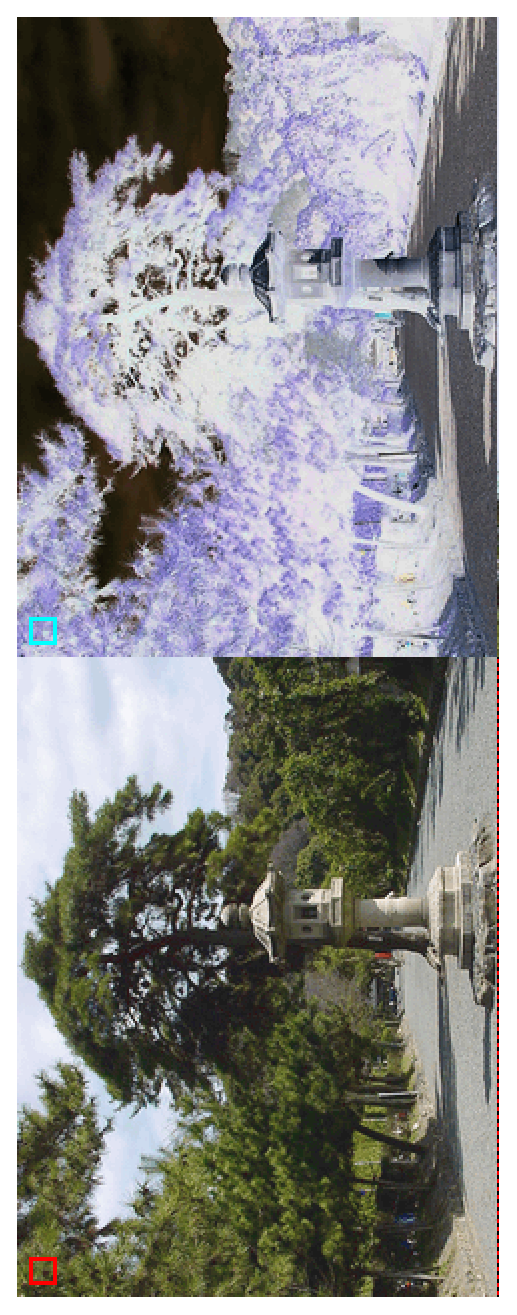
\includegraphics[angle=270,origin=b,width=0.49\textwidth]{tone_curve.eps}
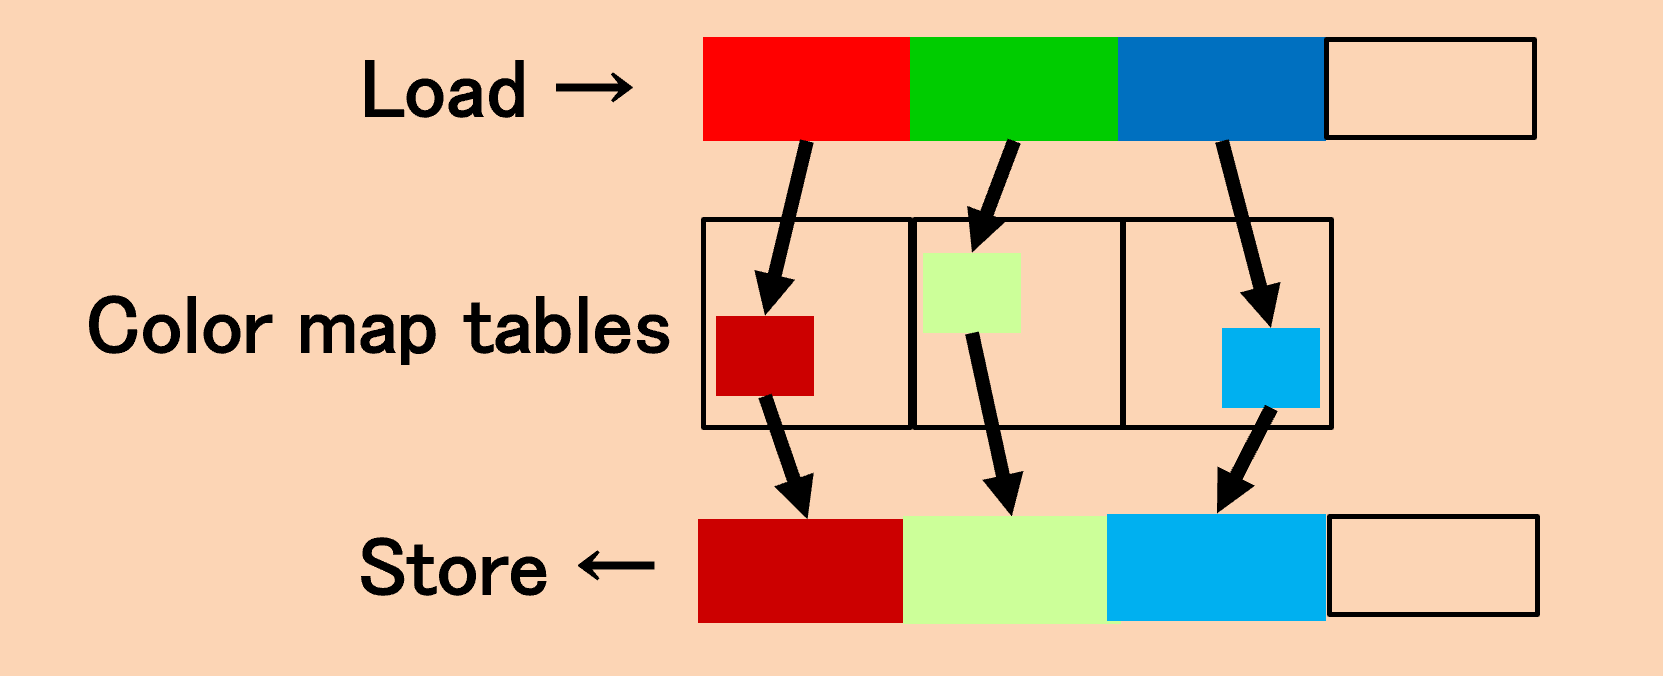
\includegraphics[angle=270,origin=b,width=0.46\textwidth]{tone1.eps}
\caption{Tone curve}
\end{figure}

\subsection{Describing algorithms in C}

\begin{screen}
\footnotesize
\begin{verbatim}
/* CPU */
for (row=0; row<HT; row++) {
  for (col=0; col<WD; col++) {
    Uint pix = hin[row*WD+col];
    hout0[row*WD+col]
      = ((ht)[pix>>24])<<24 | (ht[256+((pix>>16)&255)])<<16 | (ht[512+((pix>>8)&255)])<<8;
  }
}
\end{verbatim}
\end{screen}

\subsection{CUDA algorithm description}

\begin{screen}
\scriptsize
\begin{verbatim}
/* GPU */
if (cudaSuccess != cudaMemcpy(din, hin, sizeof(Uint)*WD*HT, cudaMemcpyHostToDevice))
  { printf("can't cudaMemcpy\n"); exit(1); }
if (cudaSuccess != cudaMemcpy(dt, ht, sizeof(Uint)*256*3, cudaMemcpyHostToDevice))
  { printf("can't cudaMemcpy\n"); exit(1); }
dim3 Thread  = dim3(THREADX, THREADY, 1);
dim3 Block   = dim3(BLOCKX, BLOCKY, 1);
tone_curve<<<Block,Thread>>>(dout, din, dt); /* search triangle in {frontier,next} */
if (cudaSuccess != cudaMemcpy(hout1, dout, sizeof(Uint)*WD*HT, cudaMemcpyDeviceToHost))
  { printf("can't cudaMemcpy\n"); exit(1); }
__global__ void tone_curve(Uint *out, Uint *in, Uchar *t)
{
  int row, col;
  row = blockIdx.y*blockDim.y + threadIdx.y;
  col = blockIdx.x*blockDim.x + threadIdx.x;
  Uint pix = in[row*WD+col];
  out[row*WD+col] = ((t)[pix>>24])<<24 | (t[256+((pix>>16)&255)])<<16 | (t[512+((pix>>8)&255)])<<8;
  __syncthreads();
}
\end{verbatim}
\end{screen}

\clearpage

\subsection{C language description for IMAX (1 pixel per cycle)}

\begin{screen}
\scriptsize
\begin{verbatim}
void tone_curve(r, d, t)
     unsigned int *r, *d;
     unsigned char *t;
{
  Ull  t1 = t;
  Ull  t2 = t+256;
  Ull  t3 = t+512;
  Ull  BR[16][4][4]; /* output registers in each unit */
  Ull  r0, r1, r2, r3, r4, r5, r6, r7, r8, r9, r10, r11, r12, r13, r14, r15,
       r16, r17, r18, r19, r20, r21, r22, r23, r24, r25, r26, r27, r28, r29, r30, r31;
  int loop=WD;
//EMAX5A begin tone_curve mapdist=0
  while (loop--) {
    mop(OP_LDWR,  1, &BR[0][1][1], (Ull)(r++), 0LL,         MSK_D0, (Ull)r, 320, 0,0, (Ull)NULL, 320);/* stage#0 */
    mop(OP_LDBR,  1, &BR[1][1][1], (Ull)t1,    BR[0][1][1], MSK_B3, (Ull)t1, 64, 0,0, (Ull)NULL, 64); /* stage#1 */
    mop(OP_LDBR,  1, &BR[1][2][1], (Ull)t2,    BR[0][1][1], MSK_B2, (Ull)t2, 64, 0,0, (Ull)NULL, 64); /* stage#1 */
    mop(OP_LDBR,  1, &BR[1][3][1], (Ull)t3,    BR[0][1][1], MSK_B1, (Ull)t3, 64, 0,0, (Ull)NULL, 64); /* stage#1 */
    exe(OP_MMRG, &r1, BR[1][1][1], EXP_H3210,  BR[1][2][1], EXP_H3210, BR[1][3][1], EXP_H3210, OP_NOP, 0, OP_NOP, 0);
    mop(OP_STWR,  3, &r1,          (Ull)(d++), 0LL,         MSK_D0, (Ull)d, 320, 0,0, (Ull)NULL, 320);/* stage#2 */
  }
//EMAX5A end
}
\end{verbatim}
\end{screen}

\begin{figure}[htbp]
\center
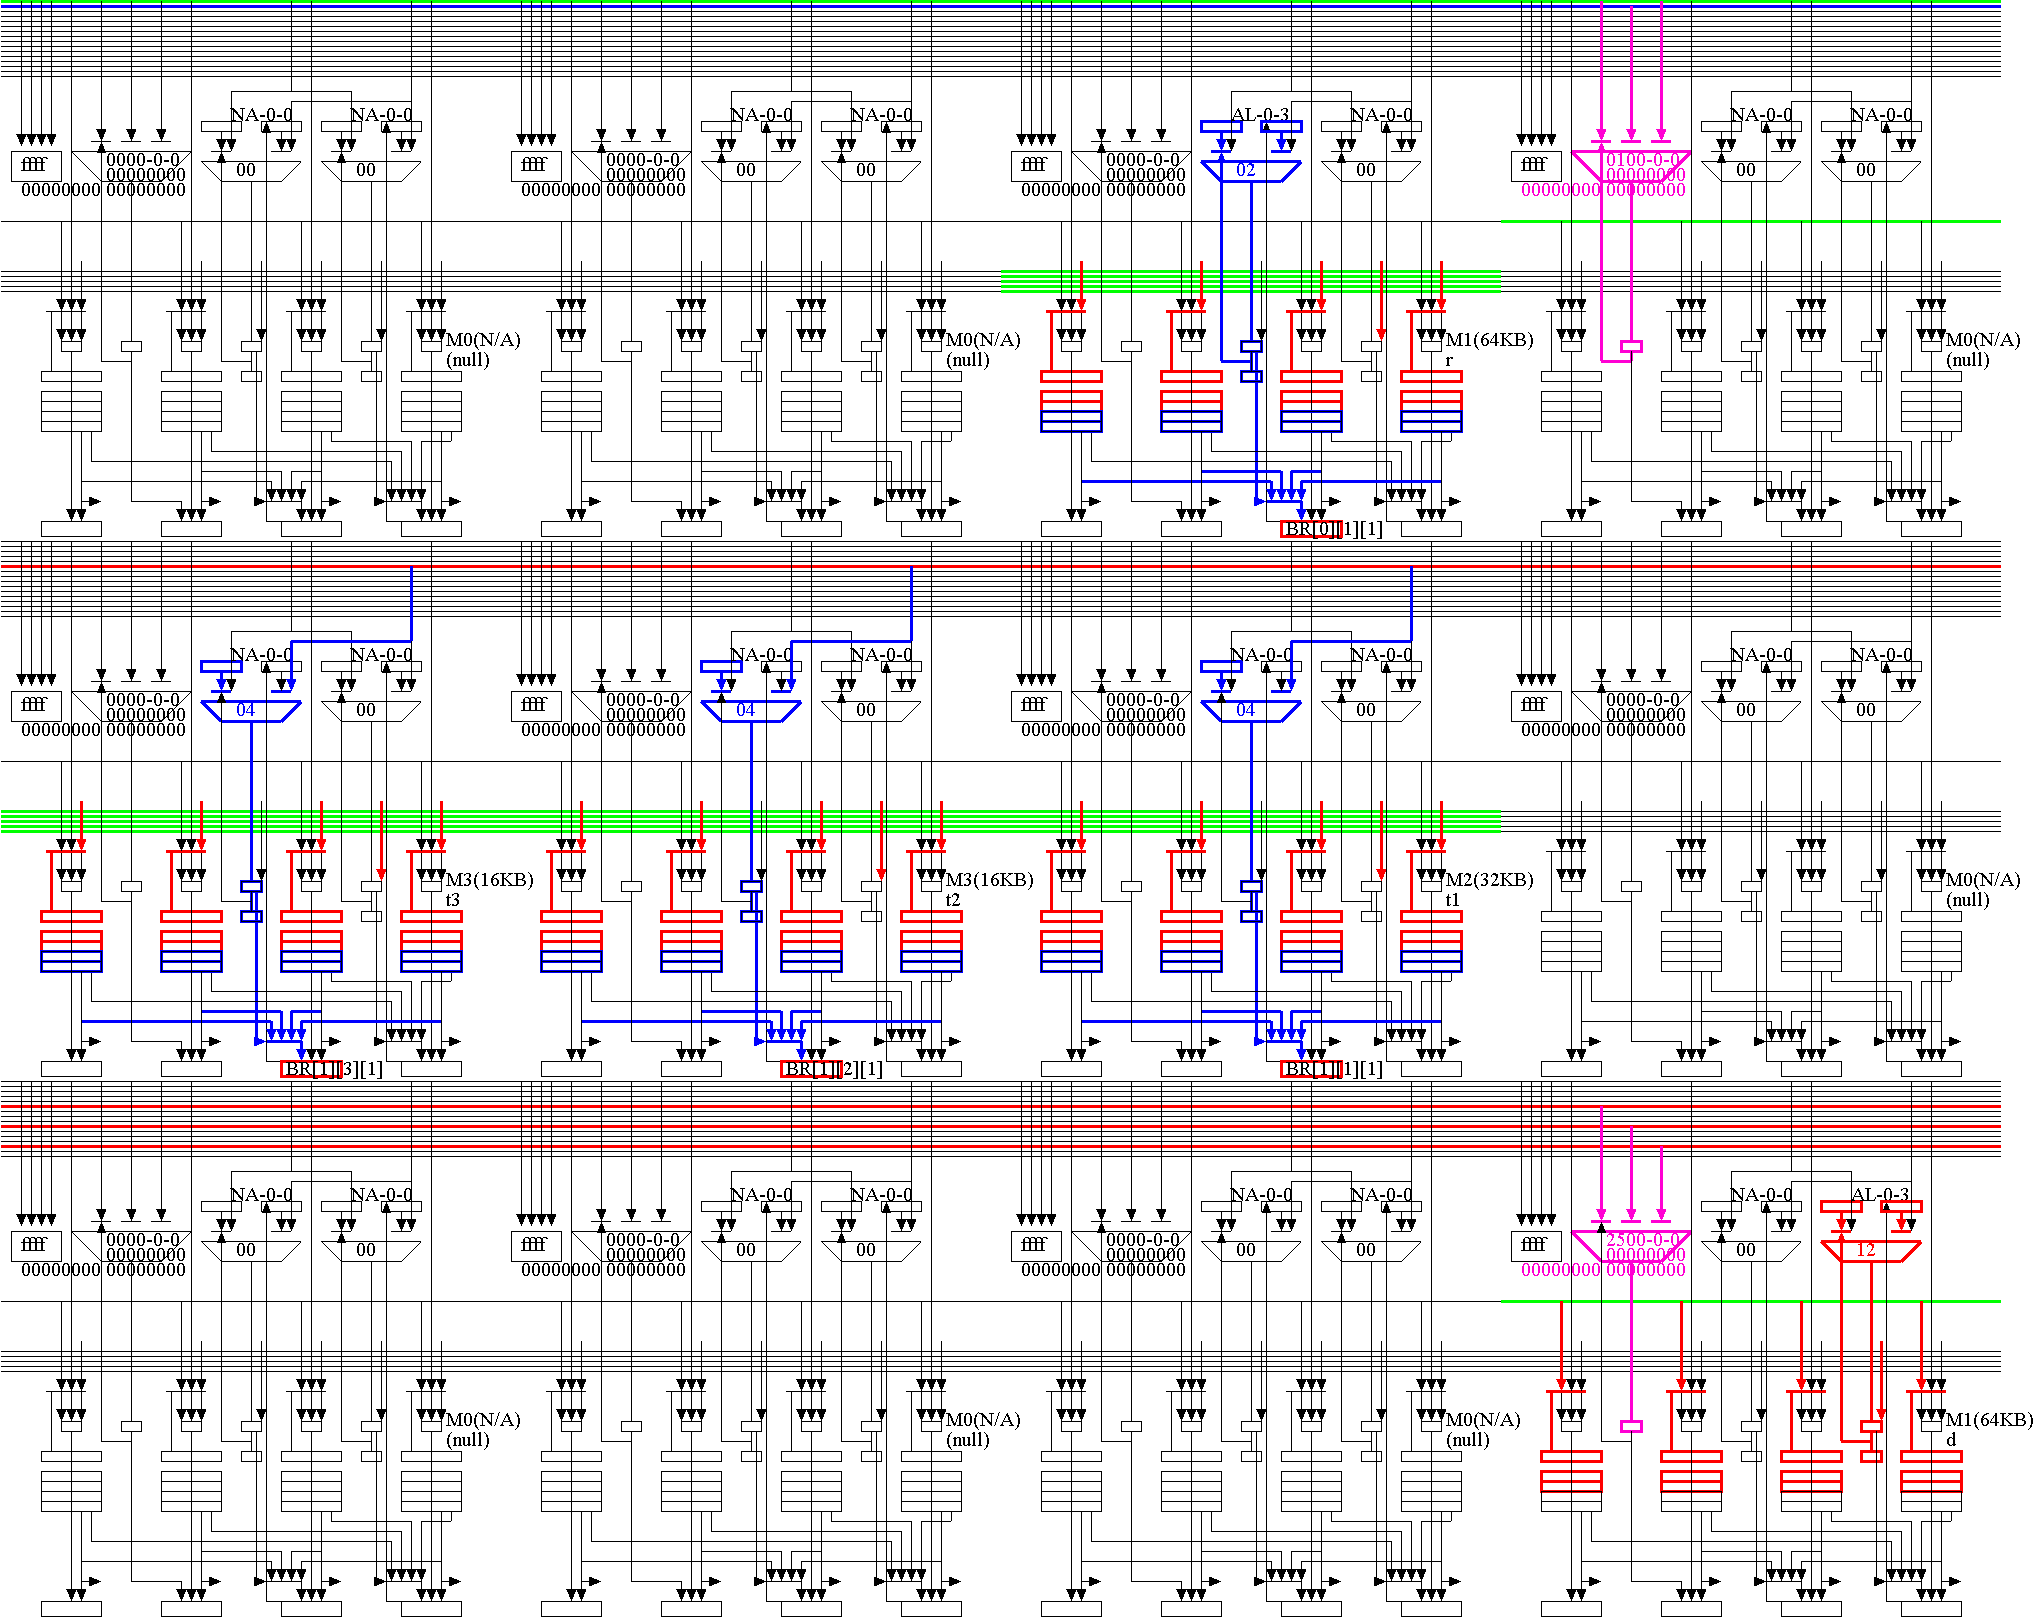
\includegraphics[angle=270,origin=b,width=0.98\textwidth]{tone3.eps}
\caption{Tone curve 1 pixel per cycle}
\end{figure}

\clearpage

\subsection{C language description for IMAX (2 pixels per cycle)}

\begin{figure}[htbp]
\center
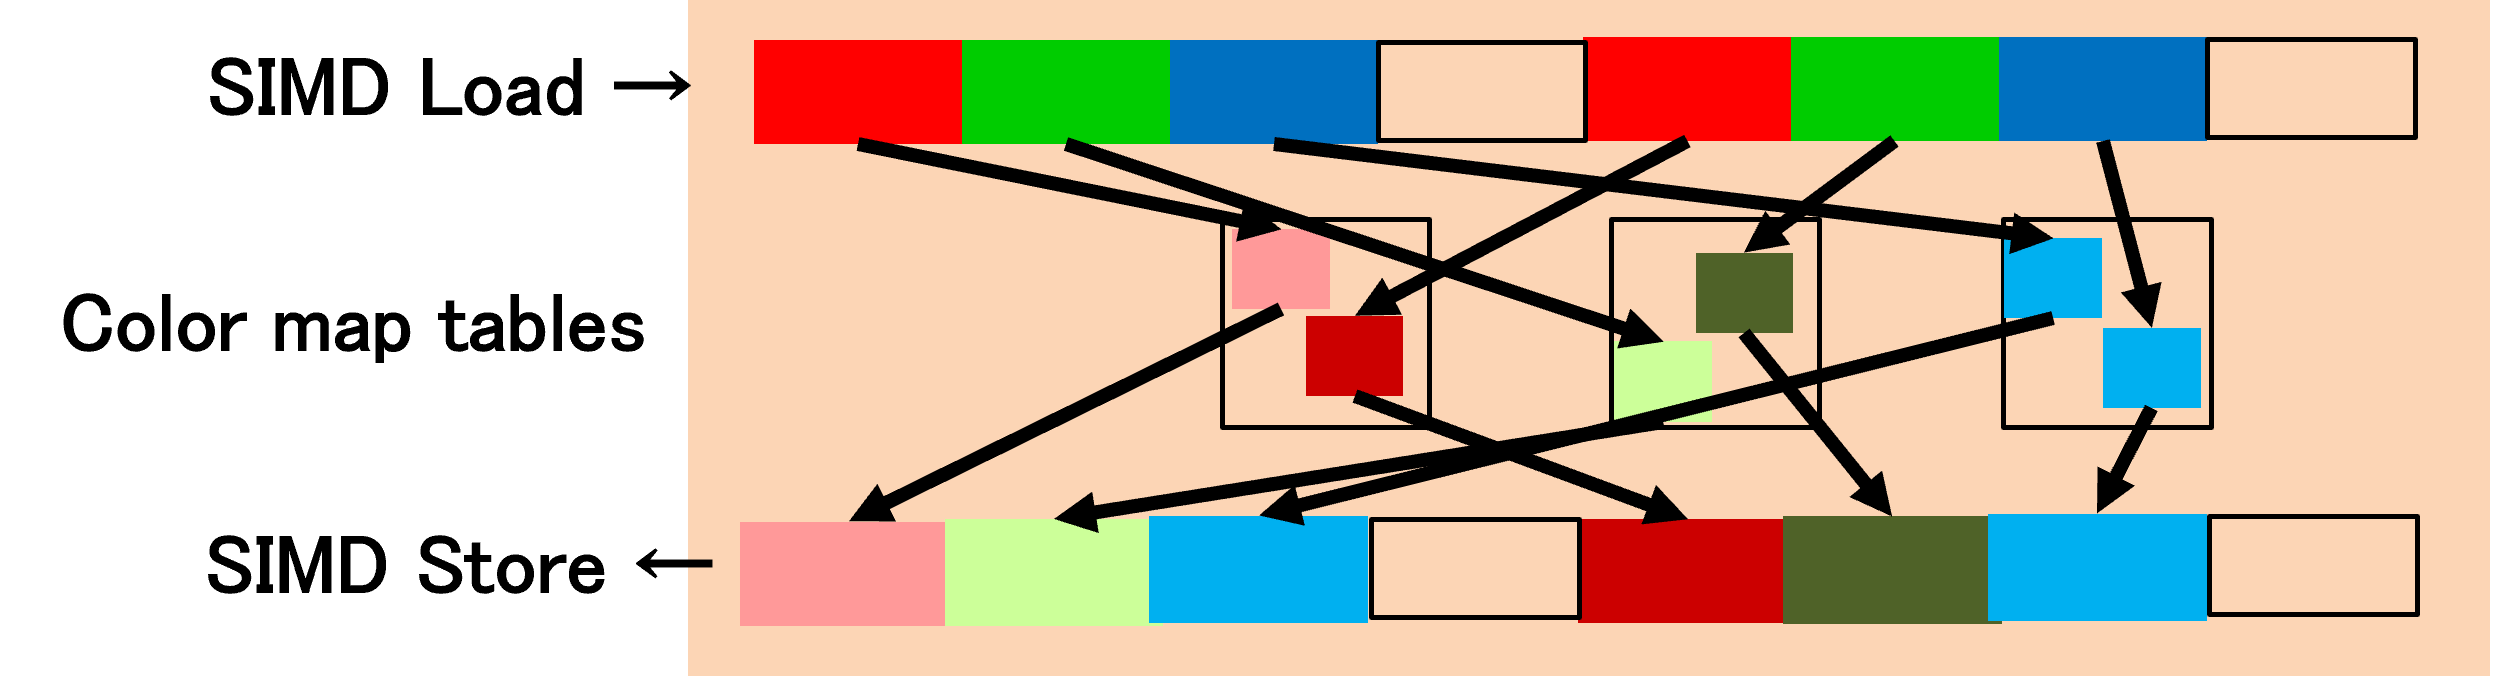
\includegraphics[angle=270,origin=b,width=0.70\textwidth]{tone2.eps}
\caption{Dual tone curve}
\end{figure}

\begin{screen}
\scriptsize
\begin{verbatim}
void tone_curve(r, d, t)
     unsigned int *r, *d;
     unsigned char *t;
{
  Ull  t1 = t;
  Ull  t2 = t+256;
  Ull  t3 = t+512;
  Ull  BR[16][4][4]; /* output registers in each unit */
  Ull  r0, r1, r2, r3, r4, r5, r6, r7, r8, r9, r10, r11, , r31;
  int loop=WD/2;
//EMAX5A begin tone_curve mapdist=0
  while (loop--) {
    mop(OP_LDR,   1, &BR[0][1][1], (Ull)(rr++), 0LL,        MSK_D0, (Ull)r, 320,  0,  0, (Ull)NULL,320);   /* stage#0 */
    mop(OP_LDBR,  1, &BR[1][1][1], (Ull)t1,    BR[0][1][1], MSK_B3, (Ull)t1, 64,  0,  0, (Ull)NULL, 64);   /* stage#1 */
    mop(OP_LDBR,  1, &BR[1][1][0], (Ull)t1,    BR[0][1][1], MSK_B7, (Ull)t1, 64,  0,  0, (Ull)NULL, 64);   /* stage#1 */
    mop(OP_LDBR,  1, &BR[1][2][1], (Ull)t2,    BR[0][1][1], MSK_B2, (Ull)t2, 64,  0,  0, (Ull)NULL, 64);   /* stage#1 */
    mop(OP_LDBR,  1, &BR[1][2][0], (Ull)t2,    BR[0][1][1], MSK_B6, (Ull)t2, 64,  0,  0, (Ull)NULL, 64);   /* stage#1 */
    mop(OP_LDBR,  1, &BR[1][3][1], (Ull)t3,    BR[0][1][1], MSK_B1, (Ull)t3, 64,  0,  0, (Ull)NULL, 64);   /* stage#1 */
    mop(OP_LDBR,  1, &BR[1][3][0], (Ull)t3,    BR[0][1][1], MSK_B5, (Ull)t3, 64,  0,  0, (Ull)NULL, 64);   /* stage#1 */
    exe(OP_CCAT,  &r1, BR[1][1][0], EXP_H3210, BR[1][1][1], EXP_H3210,        0LL, EXP_H3210, OP_NOP, 0LL, OP_NOP, 0LL);
    exe(OP_CCAT,  &r2, BR[1][2][0], EXP_H3210, BR[1][2][1], EXP_H3210,        0LL, EXP_H3210, OP_NOP, 0LL, OP_NOP, 0LL);
    exe(OP_CCAT,  &r3, BR[1][3][0], EXP_H3210, BR[1][3][1], EXP_H3210,        0LL, EXP_H3210, OP_NOP, 0LL, OP_NOP, 0LL);
    exe(OP_MMRG,  &r0,          r1, EXP_H3210, r2, EXP_H3210, r3, EXP_H3210, OP_NOP, 0LL, OP_NOP, 0LL);
    mop(OP_STR,   3, &r0,          (Ull)(dd++), 0LL,        MSK_D0, (Ull)d, 320,  0,  0, (Ull)NULL,320);   /* stage#2 */
  }
//EMAX5A end
}
\end{verbatim}
\end{screen}

\begin{figure}[htbp]
\center
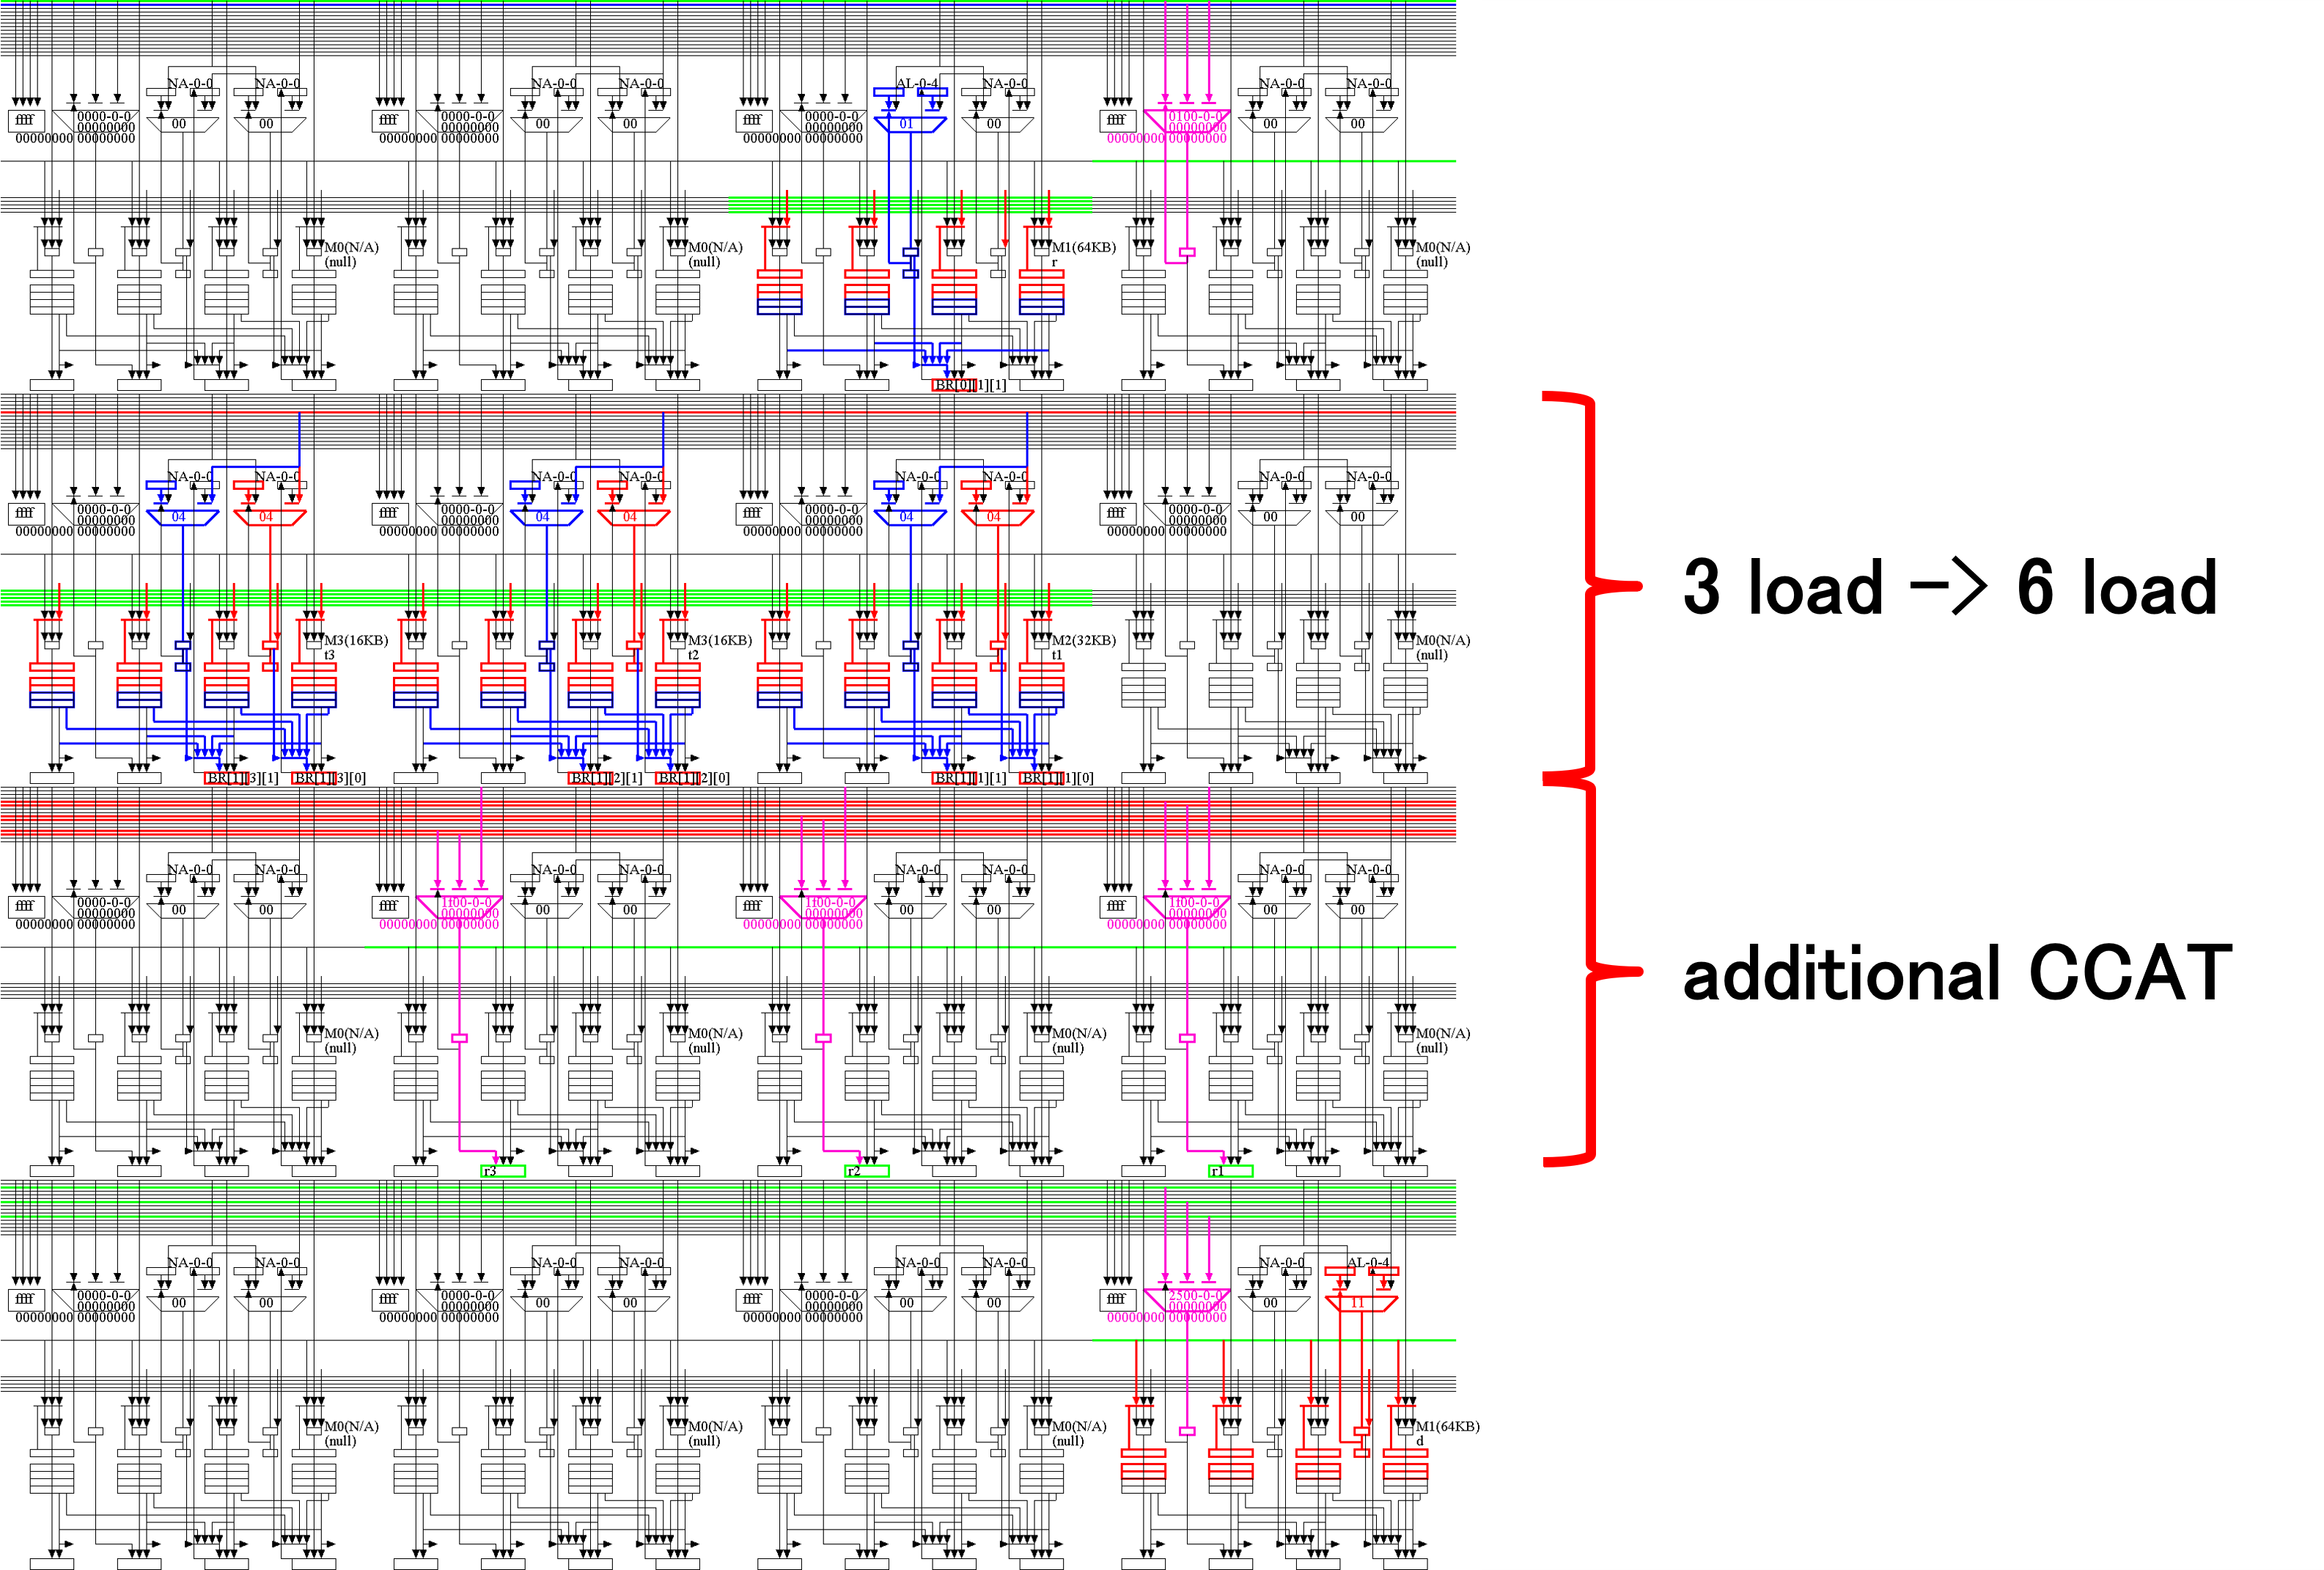
\includegraphics[angle=270,origin=b,width=0.96\textwidth]{tone4.eps}
\caption{Tone curve 2 pixels per cycle}
\end{figure}

\clearpage

\subsection{C language description for IMAX (multi-stage use, double loop batch execution, multi-chip execution)}

\begin{screen}
\scriptsize
\begin{verbatim}
void tone_curve(Uint *r, Uint *d, Uchar *t) /* R, D, lut */
{
#define NCHIP     1
#define RMGRP     6
#define OMAP     10
#define PAD       0
#define RRANGE   ((HT-PAD*2)/NCHIP/OMAP)
  int i;
  for(i=0; i<256; i++) {
    t[i+  0] = 0xff-i;
    t[i+256] = 0xff-i;
    t[i+512] = 0xff-i;
  }
  Ull  top, rofs, cofs, oc, pofs;
  Ull  t1 = t;
  Ull  t2 = t+256;
  Ull  t3 = t+512;
  Ull  CHIP;
  Ull  LOOP1, LOOP0;
  Ull  INIT1, INIT0;
  Ull  AR[64][4];                     /* output of EX     in each unit */
  Ull  BR[64][4][4];                  /* output registers in each unit */
  Ull  r0, r1, r2, r3, r4, r5, r6, r7, r8, r9, r10, r11, r12, r13, r14, r15;
  Ull  r16, r17, r18, r19, r20, r21, r22, r23, r24, r25, r26, r27, r28, r29, r30, r31;
  Ull  cc0, cc1, cc2, cc3, ex0, ex1;
  for (top=0; top<RRANGE; top+=RMGRP) {
    Ull  rtop0[NCHIP], dtop0[NCHIP];
    Ull  rtop1[NCHIP], dtop1[NCHIP];
    Ull  rtop2[NCHIP], dtop2[NCHIP];
    Ull  rtop3[NCHIP], dtop3[NCHIP];
    Ull  rtop4[NCHIP], dtop4[NCHIP];
    Ull  rtop5[NCHIP], dtop5[NCHIP];
    Ull  rtop6[NCHIP], dtop6[NCHIP];
    Ull  rtop7[NCHIP], dtop7[NCHIP];
    Ull  rtop8[NCHIP], dtop8[NCHIP];
    Ull  rtop9[NCHIP], dtop9[NCHIP];
    for (CHIP=0; CHIP<NCHIP; CHIP++) { /* output channels are parallelized by multi-chip (OC/#chip) */
      rtop0[CHIP] = r+(CHIP*RRANGE*OMAP+RRANGE*0+top)*WD; dtop0[CHIP] = d+(CHIP*RRANGE*OMAP+RRANGE*0+top)*WD;
      rtop1[CHIP] = r+(CHIP*RRANGE*OMAP+RRANGE*1+top)*WD; dtop1[CHIP] = d+(CHIP*RRANGE*OMAP+RRANGE*1+top)*WD;
      rtop2[CHIP] = r+(CHIP*RRANGE*OMAP+RRANGE*2+top)*WD; dtop2[CHIP] = d+(CHIP*RRANGE*OMAP+RRANGE*2+top)*WD;
      rtop3[CHIP] = r+(CHIP*RRANGE*OMAP+RRANGE*3+top)*WD; dtop3[CHIP] = d+(CHIP*RRANGE*OMAP+RRANGE*3+top)*WD;
      rtop4[CHIP] = r+(CHIP*RRANGE*OMAP+RRANGE*4+top)*WD; dtop4[CHIP] = d+(CHIP*RRANGE*OMAP+RRANGE*4+top)*WD;
      rtop5[CHIP] = r+(CHIP*RRANGE*OMAP+RRANGE*5+top)*WD; dtop5[CHIP] = d+(CHIP*RRANGE*OMAP+RRANGE*5+top)*WD;
      rtop6[CHIP] = r+(CHIP*RRANGE*OMAP+RRANGE*6+top)*WD; dtop6[CHIP] = d+(CHIP*RRANGE*OMAP+RRANGE*6+top)*WD;
      rtop7[CHIP] = r+(CHIP*RRANGE*OMAP+RRANGE*7+top)*WD; dtop7[CHIP] = d+(CHIP*RRANGE*OMAP+RRANGE*7+top)*WD;
      rtop8[CHIP] = r+(CHIP*RRANGE*OMAP+RRANGE*8+top)*WD; dtop8[CHIP] = d+(CHIP*RRANGE*OMAP+RRANGE*8+top)*WD;
      rtop9[CHIP] = r+(CHIP*RRANGE*OMAP+RRANGE*9+top)*WD; dtop9[CHIP] = d+(CHIP*RRANGE*OMAP+RRANGE*9+top)*WD;
    }
//EMAX5A begin tone_curve mapdist=0
    for (CHIP=0; CHIP<NCHIP; CHIP++) { /* output channels are parallelized by multi-chip (OC/#chip) */
/*2*/for (INIT1=1,LOOP1=RMGRP,rofs=0-WD*4; LOOP1--; INIT1=0) {     /* stage#0 *//* mapped to FOR() on BR[63][1][0] */
 /*1*/for (INIT0=1,LOOP0=WD,cofs=0-4; LOOP0--; INIT0=0) {          /* stage#0 *//* mapped to FOR() on BR[63][0][0] */
       exe(OP_ADD,  &cofs, INIT0?cofs:cofs, EXP_H3210, 4, EXP_H3210, 0,EXP_H3210,OP_AND,0x0ffffffffLL,OP_NOP,0);/* s#0*/
       exe(OP_ADD,  &rofs, rofs, EXP_H3210, INIT0?WD*4:0, EXP_H3210, 0,EXP_H3210,OP_NOP,0, OP_NOP, 0);          /* s#0*/
       exe(OP_ADD,  &pofs, rofs, EXP_H3210, cofs, EXP_H3210, 0,EXP_H3210, OP_AND,0x000000ffffffffLL, OP_NOP, 0);/* s#1*/
       /*map0*/
       mop(OP_LDWR, 1, &BR[2][1][1], rtop0[CHIP], pofs,  MSK_D0, rtop0[CHIP], WD*RMGRP,0,0,NULL,WD*RMGRP);      /* s#2*/
       mop(OP_LDBR, 1, &BR[3][1][1], t1,    BR[2][1][1], MSK_B3, t1, 256/4,  0,  0, NULL, 256/4);               /* s#3*/
       mop(OP_LDBR, 1, &BR[3][2][1], t2,    BR[2][1][1], MSK_B2, t2, 256/4,  0,  0, NULL, 256/4);               /* s#3*/
       mop(OP_LDBR, 1, &BR[3][3][1], t3,    BR[2][1][1], MSK_B1, t3, 256/4,  0,  0, NULL, 256/4);               /* s#3*/
       exe(OP_MMRG, &r1,BR[3][1][1], EXP_H3210, BR[3][2][1],EXP_H3210, BR[3][3][1],EXP_H3210,OP_NOP,0,OP_NOP,0);/* s#3*/
       mop(OP_STWR, 3, &r1,          dtop0[CHIP], pofs,  MSK_D0, dtop0[CHIP], WD*RMGRP,0,0,NULL,WD*RMGRP);      /* s#3*/
         :
       /*map9*/
       mop(OP_LDWR, 1, &BR[20][1][1],rtop9[CHIP], pofs,  MSK_D0, rtop9[CHIP], WD*RMGRP,0,0,NULL,WD*RMGRP);      /*s#20*/
       mop(OP_LDBR, 1, &BR[21][1][1],t1,    BR[20][1][1],MSK_B3, t1, 256/4,  0,  0, NULL, 256/4);               /*s#21*/
       mop(OP_LDBR, 1, &BR[21][2][1],t2,    BR[20][1][1],MSK_B2, t2, 256/4,  0,  0, NULL, 256/4);               /*s#21*/
       mop(OP_LDBR, 1, &BR[21][3][1],t3,    BR[20][1][1],MSK_B1, t3, 256/4,  0,  0, NULL, 256/4);               /*s#21*/
       exe(OP_MMRG, &r1,BR[21][1][1],EXP_H3210,BR[21][2][1],EXP_H3210,BR[21][3][1],EXP_H3210,OP_NOP,0,OP_NOP,0);/*s#21*/
       mop(OP_STWR, 3, &r1,          dtop9[CHIP], pofs,  MSK_D0, dtop9[CHIP], WD*RMGRP,0,0,NULL,WD*RMGRP);      /*s#21*/
      }
     }
    }
//EMAX5A end
  }
//EMAX5A drain_dirty_lmm
}
\end{verbatim}
\end{screen}

\clearpage

\section{Basics}

\subsection{FFT}

\shabox{
\leftline{cent\% make -f Makefile-csim.emax6+dma all clean}
\leftline{cent\% ../../src/csim/csim -x fft-csim.emax6+dma 4 4096}
}

\shabox{
\leftline{zynq\% make -f Makefile-zynq.emax6+dma all clean}
\leftline{zynq\% ./fft-zynq.emax6+dma 4 4096}
}

\subsubsection{Simple implementation}

In the case LMM=8K*4byte*2=64KB, FFT for 8192 elements can be executed.
In the case LMM=64K*4byte*2=512KB, FFT for 65526 elements can be executed.

\begin{screen}
\tiny
\begin{verbatim}
printf("<<<ORIG>>>\n");
reset_nanosec();
BlockEnd = 1;
for (BlockSize=2; BlockSize<=NumSamples; BlockSize<<=1) {
  for (i=0; i<NumSamples; i+=BlockSize) {
    for (j=i,n=0; n<BlockEnd; j++,n++) {
      k   = j + BlockEnd;
      idx = n + BlockEnd;
      tr = art[idx]*RealOut[k] - ait[idx]*ImagOut[k];
      ti = art[idx]*ImagOut[k] + ait[idx]*RealOut[k];
      RealOut[k] = RealOut[j] - tr;
      ImagOut[k] = ImagOut[j] - ti;
      RealOut[j] += tr;
      ImagOut[j] += ti;
  } }
  BlockEnd = BlockSize;
}
\end{verbatim}
\end{screen}

\begin{screen}
\tiny
\begin{verbatim}
  Ull  CHIP;
  Ull  LOOP1, LOOP0;
  Ull  INIT1, INIT0;
  Ull  AR[64][4];                     /* output of EX     in each unit */
  Ull  BR[64][4][4];                  /* output registers in each unit */
  Ull  r0, r1, r2, r3, r4, r5, r6, r7, r8, r9, r10, r11, r12, r13, r14, r15;
  Ull  r16, r17, r18, r19, r20, r21, r22, r23, r24, r25, r26, r27, r28, r29, r30, r31;
  Ull  cc0, cc1, cc2, cc3, ex0, ex1;
  Ull  ar, ai, rok, iok, roj, ioj;
  Ull  tr0, ti0, tr1, ti1, roj1, ioj1;

  printf("<<<IMAX>>> NumSamples=%d (LMM should be >= %dB)\n", NumSamples, NumSamples*4*2);
  reset_nanosec();

#define fft_core0(r) \
          exe(OP_ADD,     &j,         i,        EXP_H3210,  n,       EXP_H3210, 0LL,          EXP_H3210, OP_NOP, 0LL, OP_SLL, 2LL); /* stage#1 */\
          exe(OP_ADD3,    &k,         i,        EXP_H3210,  n,       EXP_H3210, BlockEnd,     EXP_H3210, OP_NOP, 0LL, OP_SLL, 2LL); /* stage#1 */\
          exe(OP_ADD3,    &idx,       0LL,      EXP_H3210,  n,       EXP_H3210, BlockEnd,     EXP_H3210, OP_NOP, 0LL, OP_SLL, 2LL); /* stage#1 */\
          exe(OP_NOP,     &AR[r][0],  0LL,      EXP_H3210,  0LL,     EXP_H3210, 0LL,          EXP_H3210, OP_NOP, 0LL, OP_NOP, 0LL); /* stage#2 [2][0]     */\
          mop(OP_LDWR, 3, &rok,       RealOut,  k,          MSK_D0,  RealOut,   NumSamples,   0, 1,  NULL,  NumSamples);            /* stage#2 RealOut[k] */\
          mop(OP_LDWR, 3, &roj,       j,        RealOut,    MSK_D0,  RealOut,   NumSamples,   0, 1,  NULL,  NumSamples);            /* stage#2 RealOut[j] */\
          exe(OP_NOP,     &AR[r][2],  0LL,      EXP_H3210,  0LL,     EXP_H3210, 0LL,          EXP_H3210, OP_NOP, 0LL, OP_NOP, 0LL); /* stage#2 [2][2]     */\
          mop(OP_LDWR, 3, &iok,       ImagOut,  k,          MSK_D0,  ImagOut,   NumSamples,   0, 1,  NULL,  NumSamples);            /* stage#2 ImagOut[k] */\
          mop(OP_LDWR, 3, &ioj,       j,        ImagOut,    MSK_D0,  ImagOut,   NumSamples,   0, 1,  NULL,  NumSamples)             /* stage#2 ImagOut[j] */
#define fft_core1(r) \
          exe(OP_NOP,     &AR[r][0],  0LL,      EXP_H3210,  0LL,     EXP_H3210, 0LL,          EXP_H3210, OP_NOP, 0LL, OP_NOP, 0LL); /* stage#3 [3][0]     */\
          mop(OP_LDWR, 3, &ar,        art,      idx,        MSK_D0,  art,       NumSamples,   0, 0,  NULL,  NumSamples);            /* stage#3 art[idx]   */\
          exe(OP_NOP,     &AR[r][2],  0LL,      EXP_H3210,  0LL,     EXP_H3210, 0LL,          EXP_H3210, OP_NOP, 0LL, OP_NOP, 0LL); /* stage#3 [3][2]     */\
          mop(OP_LDWR, 3, &ai,        ait,      idx,        MSK_D0,  ait,       NumSamples,   0, 0,  NULL,  NumSamples);            /* stage#3 ait[idx]   */\
          exe(OP_FML,     &tr0,       ar,       EXP_H3210,  rok,     EXP_H3210, 0LL,          EXP_H3210, OP_NOP, 0LL, OP_NOP, 0LL); /* stage#4 */\
          exe(OP_FML,     &ti0,       ar,       EXP_H3210,  iok,     EXP_H3210, 0LL,          EXP_H3210, OP_NOP, 0LL, OP_NOP, 0LL); /* stage#4 */\
          exe(OP_FMS,     &tr1,       tr0,      EXP_H3210,  ai,      EXP_H3210, iok,          EXP_H3210, OP_NOP, 0LL, OP_NOP, 0LL); /* stage#5 */\
          exe(OP_FMA,     &ti1,       ti0,      EXP_H3210,  ai,      EXP_H3210, rok,          EXP_H3210, OP_NOP, 0LL, OP_NOP, 0LL)  /* stage#5 */
#define fft_final(r) \
          exe(OP_FMS,     &AR[r][0],  roj,      EXP_H3210,  tr1,     EXP_H3210, 0x3f800000LL, EXP_H3210, OP_NOP, 0LL, OP_NOP, 0LL); /* stage#6 */\
          mop(OP_STWR, 3, &AR[r][0],  RealOut,  k,          MSK_D0,  RealOut,   NumSamples,   0, 0,  NULL,  NumSamples);            /* stage#6 */\
          exe(OP_FAD,     &AR[r][1],  roj,      EXP_H3210,  tr1,     EXP_H3210, 0LL,          EXP_H3210, OP_NOP, 0LL, OP_NOP, 0LL); /* stage#6 */\
          mop(OP_STWR, 3, &AR[r][1],  RealOut,  j,          MSK_D0,  RealOut,   NumSamples,   0, 0,  NULL,  NumSamples);            /* stage#6 */\
          exe(OP_FMS,     &AR[r][2],  ioj,      EXP_H3210,  ti1,     EXP_H3210, 0x3f800000LL, EXP_H3210, OP_NOP, 0LL, OP_NOP, 0LL); /* stage#6 */\
          mop(OP_STWR, 3, &AR[r][2],  ImagOut,  k,          MSK_D0,  ImagOut,   NumSamples,   0, 0,  NULL,  NumSamples);            /* stage#6 */\
          exe(OP_FAD,     &AR[r][3],  ioj,      EXP_H3210,  ti1,     EXP_H3210, 0LL,          EXP_H3210, OP_NOP, 0LL, OP_NOP, 0LL); /* stage#6 */\
          mop(OP_STWR, 3, &AR[r][3],  ImagOut,  j,          MSK_D0,  ImagOut,   NumSamples,   0, 0,  NULL,  NumSamples)             /* stage#6 */
  BlockEnd = 1;
  for (BlockSize=2; BlockSize<=NumSamples; BlockSize<<=1) {
//with-prefetch/post-drain
//EMAX5A begin imax mapdist=0
/*3*/for (CHIP=0; CHIP<NCHIP; CHIP++) {
  /*2*/for (INIT1=1,LOOP1=NumSamples/BlockSize,i=0LL<<32|(0-BlockSize)&0xffffffff; LOOP1--; INIT1=0) {
    /*1*/for (INIT0=1,LOOP0=BlockEnd,n=0LL<<32|(0-1LL)&0xffffffff; LOOP0--; INIT0=0) {
          exe(OP_ADD,     &i,     i,         EXP_H3210,   INIT0?BlockSize:0, EXP_H3210, 0LL, EXP_H3210, OP_NOP, 0LL, OP_NOP, 0LL);          /* stage#0 */
          exe(OP_ADD,     &n,     INIT0?n:n, EXP_H3210,   0LL<<32|1LL,       EXP_H3210, 0LL,          EXP_H3210, OP_NOP, 0LL, OP_NOP, 0LL); /* stage#0 */
          fft_core0(2); /* stage#2   */
          fft_core1(3); /* stage#3-5 */
          fft_final(6); /* stage#6   */
    } } }
//EMAX5A end
//EMAX5A drain_dirty_lmm
    BlockEnd = BlockSize;
  }
\end{verbatim}
\end{screen}

\begin{figure}[htbp]
\center
\epsfile{file=fourierf-imax-emax6.eps,width=1.00\textwidth}
\caption{FFT}
\end{figure}

\clearpage

\subsubsection{Pipelined implementation}

This is a pipelined FFT.  In the case LMM=4K*4byte*2*DB=64KB, FFT for 4096
elements can be executed.  In the case LMM=32K*4byte*2*DB=512KB, FFT for
32768 elements can be executed.  Intermediate LMMs are used as double
buffers.

\begin{screen}
\tiny
\begin{verbatim}
  Ull  CHIP;
  Ull  LOOP1, LOOP0, L;
  Ull  INIT1, INIT0;
  Ull  AR[64][4];                     /* output of EX     in each unit */
  Ull  BR[64][4][4];                  /* output registers in each unit */
  Ull  r0, r1, r2, r3, r4, r5, r6, r7, r8, r9, r10, r11, r12, r13, r14, r15;
  Ull  r16, r17, r18, r19, r20, r21, r22, r23, r24, r25, r26, r27, r28, r29, r30, r31;
  Ull  cc0, cc1, cc2, cc3, ex0, ex1;
  Ull  J[16], K[16], IDX[16]; /* log2(NumSamples=65536)=16�ޤ��б��� */
  Ull  BufReal[16], BufImag[16];
  Ull  ar, ai, rok, iok, roj, ioj, tr0, ti0, tr1, ti1;
  Ull  Pipeline, Lmmrotate; /* log2(NumSamples=65536)=16�󷫤��֤���,�ǽ��ʤ�LMM��,�ǽ��RealOut/ImagOut����Ǽ����� */
  printf("<<<IMAX>>> NumSamples=%d (LMM should be >= %dB)\n", NumSamples, NumSamples*4*2);
  reset_nanosec();
#define fft_core0(r, x, MASK_M, MASK_N, BS) \
        exe(OP_ADD,     &i,         L,          EXP_H3210,  L,       EXP_H3210, 0LL,          EXP_H3210, OP_AND, MASK_M, OP_NOP, 0LL); /* stage#1 i  =(L*2)&M   */\
        exe(OP_ADD,     &n,         L,          EXP_H3210,  0LL,     EXP_H3210, 0LL,          EXP_H3210, OP_AND, MASK_N, OP_NOP, 0LL); /* stage#1 n  =L    &N   */\
        exe(OP_ADD,     &J[x],      i,          EXP_H3210,  n,       EXP_H3210, 0LL,          EXP_H3210, OP_NOP, 0LL,    OP_SLL, 2LL); /* stage#2 j  =i+n       */\
        exe(OP_ADD3,    &K[x],      i,          EXP_H3210,  n,       EXP_H3210, BS,           EXP_H3210, OP_NOP, 0LL,    OP_SLL, 2LL); /* stage#2 k  =i+n+BS(2) */\
        exe(OP_ADD3,    &IDX[x],    0LL,        EXP_H3210,  n,       EXP_H3210, BS,           EXP_H3210, OP_NOP, 0LL,    OP_SLL, 2LL)  /* stage#2 idx=  n+BS(2) */
#define fft_core1(r, x) \
        exe(OP_NOP,     &AR[r][0],  0LL,        EXP_H3210,  0LL,     EXP_H3210, 0LL,          EXP_H3210, OP_NOP, 0LL,    OP_NOP, 0LL); /* stage#3 [3][0]        */\
        mop(OP_LDWR, 3, &rok,       RealIn,     K[x],       MSK_D0,  RealIn,    NumSamples,   0, 1,  NULL,  NumSamples);               /* stage#3 RealIn[k]     */\
        mop(OP_LDWR, 3, &roj,       J[x],       RealIn,     MSK_D0,  RealIn,    NumSamples,   0, 1,  NULL,  NumSamples);               /* stage#3 RealIn[j]     */\
        exe(OP_NOP,     &AR[r][2],  0LL,        EXP_H3210,  0LL,     EXP_H3210, 0LL,          EXP_H3210, OP_NOP, 0LL,    OP_NOP, 0LL); /* stage#3 [3][2]        */\
        mop(OP_LDWR, 3, &iok,       ImagIn,     K[x],       MSK_D0,  ImagIn,    NumSamples,   0, 1,  NULL,  NumSamples);               /* stage#3 ImagIn[k]     */\
        mop(OP_LDWR, 3, &ioj,       J[x],       ImagIn,     MSK_D0,  ImagIn,    NumSamples,   0, 1,  NULL,  NumSamples)                /* stage#3 ImagIn[j]     */
#define fft_core2(r, x, y, MASK_M, MASK_N, BS) \
        exe(OP_NOP,     &AR[r][0],  0LL,        EXP_H3210,  0LL,     EXP_H3210, 0LL,          EXP_H3210, OP_NOP, 0LL,    OP_NOP, 0LL); /* stage#4 [4][0]        */\
        exe(OP_ADD,     &i,         L,          EXP_H3210,  L,       EXP_H3210, 0LL,          EXP_H3210, OP_AND, MASK_M, OP_NOP, 0LL); /* stage#4 i  =(L*2)&M   */\
        mop(OP_LDWR, 3, &ar,        art,        IDX[x],     MSK_D0,  art,       NumSamples,   0, 0,  NULL,  NumSamples);               /* stage#4 art[idx]      */\
        exe(OP_NOP,     &AR[r][2],  0LL,        EXP_H3210,  0LL,     EXP_H3210, 0LL,          EXP_H3210, OP_NOP, 0LL,    OP_NOP, 0LL); /* stage#4 [4][2]        */\
        exe(OP_ADD,     &n,         L,          EXP_H3210,  0LL,     EXP_H3210, 0LL,          EXP_H3210, OP_AND, MASK_N, OP_NOP, 0LL); /* stage#4 n  = L   &N   */\
        mop(OP_LDWR, 3, &ai,        ait,        IDX[x],     MSK_D0,  ait,       NumSamples,   0, 0,  NULL,  NumSamples);               /* stage#4 ait[idx]      */\
        \
        exe(OP_ADD,     &J[y],      i,          EXP_H3210,  n,       EXP_H3210, 0LL,          EXP_H3210, OP_NOP, 0LL,    OP_SLL, 2LL); /* stage#5 j  =i+n       */\
        exe(OP_ADD3,    &K[y],      i,          EXP_H3210,  n,       EXP_H3210, BS,           EXP_H3210, OP_NOP, 0LL,    OP_SLL, 2LL); /* stage#5 k  =i+n+BS(2) */\
        exe(OP_FML,     &tr0,       ar,         EXP_H3210,  rok,     EXP_H3210, 0LL,          EXP_H3210, OP_NOP, 0LL,    OP_NOP, 0LL); /* stage#5 */\
        exe(OP_FML,     &ti0,       ar,         EXP_H3210,  iok,     EXP_H3210, 0LL,          EXP_H3210, OP_NOP, 0LL,    OP_NOP, 0LL); /* stage#5 */\
        \
        exe(OP_ADD3,    &IDX[y],    0LL,        EXP_H3210,  n,       EXP_H3210, BS,           EXP_H3210, OP_NOP, 0LL,    OP_SLL, 2LL); /* stage#6 idx=  n+BS(2) */\
        exe(OP_FMS,     &tr1,       tr0,        EXP_H3210,  ai,      EXP_H3210, iok,          EXP_H3210, OP_NOP, 0LL,    OP_NOP, 0LL); /* stage#6 */\
        exe(OP_FMA,     &ti1,       ti0,        EXP_H3210,  ai,      EXP_H3210, rok,          EXP_H3210, OP_NOP, 0LL,    OP_NOP, 0LL)  /* stage#6 */
#define fft_core3(r, x, y) \
        exe(OP_FMS,     &AR[r][0],  roj,        EXP_H3210,  tr1,     EXP_H3210, 0x3f800000LL, EXP_H3210, OP_NOP, 0LL,    OP_NOP, 0LL); /* stage#7 */\
        mop(OP_STWR, 3, &AR[r][0],  BufReal[x], K[x],       MSK_D0,  BufReal[x],0LL,          0, 0,  NULL,  0LL);                      /* stage#7 */\
        mop(OP_LDWR, 3, &rok,       K[y],       BufReal[y], MSK_D0,  BufReal[x],0LL,          0, 0,  NULL,  0LL);                      /* stage#7 BufReal[k] */\
        exe(OP_FAD,     &AR[r][1],  roj,        EXP_H3210,  tr1,     EXP_H3210, 0LL,          EXP_H3210, OP_NOP, 0LL,    OP_NOP, 0LL); /* stage#7 */\
        mop(OP_STWR, 3, &AR[r][1],  BufReal[x], J[x],       MSK_D0,  BufReal[x],0LL,          0, 0,  NULL,  0LL);                      /* stage#7 */\
        mop(OP_LDWR, 3, &roj,       J[y],       BufReal[y], MSK_D0,  BufReal[x],0LL,          0, 0,  NULL,  0LL);                      /* stage#7 BufReal[j] */\
        exe(OP_FMS,     &AR[r][2],  ioj,        EXP_H3210,  ti1,     EXP_H3210, 0x3f800000LL, EXP_H3210, OP_NOP, 0LL,    OP_NOP, 0LL); /* stage#7 */\
        mop(OP_STWR, 3, &AR[r][2],  BufImag[x], K[x],       MSK_D0,  BufImag[x],0LL,          0, 0,  NULL,  0LL);                      /* stage#7 */\
        mop(OP_LDWR, 3, &iok,       K[y],       BufImag[y], MSK_D0,  BufImag[x],0LL,          0, 0,  NULL,  0LL);                      /* stage#7 BufImag[k] */\
        exe(OP_FAD,     &AR[r][3],  ioj,        EXP_H3210,  ti1,     EXP_H3210, 0LL,          EXP_H3210, OP_NOP, 0LL,    OP_NOP, 0LL); /* stage#7 */\
        mop(OP_STWR, 3, &AR[r][3],  BufImag[x], J[x],       MSK_D0,  BufImag[x],0LL,          0, 0,  NULL,  0LL);                      /* stage#7 */\
        mop(OP_LDWR, 3, &ioj,       J[y],       BufImag[y], MSK_D0,  BufImag[x],0LL,          0, 0,  NULL,  0LL)                       /* stage#7 BufImag[j] */
#define fft_final(r, x) \
        exe(OP_FMS,     &AR[r][0],  roj,        EXP_H3210,  tr1,     EXP_H3210, 0x3f800000LL, EXP_H3210, OP_NOP, 0LL,    OP_NOP, 0LL); /* stage#7 */\
        mop(OP_STWR, 3, &AR[r][0],  RealOut,    K[x],       MSK_D0,  RealOut,   NumSamples,   0, 0,  NULL,  NumSamples);               /* stage#7 */\
        exe(OP_FAD,     &AR[r][1],  roj,        EXP_H3210,  tr1,     EXP_H3210, 0LL,          EXP_H3210, OP_NOP, 0LL,    OP_NOP, 0LL); /* stage#7 */\
        mop(OP_STWR, 3, &AR[r][1],  RealOut,    J[x],       MSK_D0,  RealOut,   NumSamples,   0, 0,  NULL,  NumSamples);               /* stage#7 */\
        exe(OP_FMS,     &AR[r][2],  ioj,        EXP_H3210,  ti1,     EXP_H3210, 0x3f800000LL, EXP_H3210, OP_NOP, 0LL,    OP_NOP, 0LL); /* stage#7 */\
        mop(OP_STWR, 3, &AR[r][2],  ImagOut,    K[x],       MSK_D0,  ImagOut,   NumSamples,   0, 0,  NULL,  NumSamples);               /* stage#7 */\
        exe(OP_FAD,     &AR[r][3],  ioj,        EXP_H3210,  ti1,     EXP_H3210, 0LL,          EXP_H3210, OP_NOP, 0LL,    OP_NOP, 0LL); /* stage#7 */\
        mop(OP_STWR, 3, &AR[r][3],  ImagOut,    J[x],       MSK_D0,  ImagOut,   NumSamples,   0, 0,  NULL,  NumSamples)                /* stage#7 */
  for (Pipeline=0; Pipeline<NumBits; Pipeline++) {
    /* 0: buf[0]=[(0+4-0)%4]:0 buf[1]=[(1+4-0)%4]:1 buf[2]=[(2+4-0)%4]:2 buf[3]=[(3+4-0)%4]:3 */
    /* 1: buf[0]=[(0+4-1)%4]:3 buf[1]=[(1+4-1)%4]:0 buf[2]=[(2+4-1)%4]:1 buf[3]=[(3+4-1)%4]:2 */
    /* 2: buf[0]=[(0+4-2)%4]:2 buf[1]=[(1+4-2)%4]:3 buf[2]=[(2+4-2)%4]:0 buf[3]=[(3+4-2)%4]:1 */
    for (Lmmrotate=0; Lmmrotate<=NumBits; Lmmrotate++) {
      BufReal[Lmmrotate] = &pseudoLMM[NumSamples*(((Lmmrotate+NumBits+1-Pipeline)%(NumBits+1))*2  )];
      BufImag[Lmmrotate] = &pseudoLMM[NumSamples*(((Lmmrotate+NumBits+1-Pipeline)%(NumBits+1))*2+1)];
    }
//EMAX5A begin pipeline mapdist=0
/*3*/for (CHIP=0; CHIP<NCHIP; CHIP++) {
 /*1*/for (INIT0=1,LOOP0=NumSamples/2,L=0LL<<32|(0-1LL)&0xffffffff; LOOP0--; INIT0=0) { /* NumSamples<=4096 */
        exe(OP_ADD,     &L,         L,          EXP_H3210,  0LL<<32|1LL, EXP_H3210, 0LL,      EXP_H3210, OP_NOP, 0LL,    OP_NOP, 0LL); /* stage#0 */
#if (H==4096)
        fft_core0( 1,  0,     0xfffeLL, 0x0000LL,    1LL); /* stage#1-2   */
        fft_core1( 3,  0);                                 /* stage#3     */
        fft_core2( 4,  0,  1, 0xfffcLL, 0x0001LL,    2LL); /* stage#4-6   */
        fft_core3( 7,  0,  1);                             /* stage#7     */
        fft_core2( 8,  1,  2, 0xfff8LL, 0x0003LL,    4LL); /* stage#8-10  */
        fft_core3(11,  1,  2);                             /* stage#11    */
        fft_core2(12,  2,  3, 0xfff0LL, 0x0007LL,    8LL); /* stage#12-14 */
        fft_core3(15,  2,  3);                             /* stage#15    */
        fft_core2(16,  3,  4, 0xffe0LL, 0x000fLL,   16LL); /* stage#16-18 */
        fft_core3(19,  3,  4);                             /* stage#19    */
        fft_core2(20,  4,  5, 0xffc0LL, 0x001fLL,   32LL); /* stage#20-22 */
        fft_core3(23,  4,  5);                             /* stage#23    */
        fft_core2(24,  5,  6, 0xff80LL, 0x003fLL,   64LL); /* stage#24-26 */
        fft_core3(27,  5,  6);                             /* stage#27    */
        :
        fft_core2(44, 10, 11, 0xf000LL, 0x07ffLL, 2048LL); /* stage#44-46 */
        fft_core3(47, 10, 11);                             /* stage#47    */
        fft_core2(48, 11, 12, 0xe000LL, 0x0fffLL, 4096LL); /* stage#48-50 */
        fft_final(51, 11);                                 /* stage#51    */
#endif
    } }
//EMAX5A end
//EMAX5A drain_dirty_lmm
  }
\end{verbatim}
\end{screen}

\begin{figure}[htbp]
\center
\epsfile{file=fourierf-pipeline-emax6.eps,width=1.00\textwidth}
\caption{FFT}
\end{figure}

\clearpage

\subsection{Merge sort}

\shabox{
\leftline{cent\% make -f Makefile-csim.emax6+dma all clean}
\leftline{cent\% ../../src/csim/csim -x sort-merge-csim.emax6+dma 4096}
}

\shabox{
\leftline{zynq\% make -f Makefile-zynq.emax6+dma all clean}
\leftline{zynq\% ./sort-merge-zynq.emax6+dma 4096}
}

\vskip .1in

In the case LMM=4K*8byte*DB=64KB, pipelined merge sort for 4096 elements can
be executed.  In the case LMM=32K*8byte*DB=512KB, pipelined merge sort for
32768 elements can be executed.  Intermediate LMMs are used as double
buffers.  The size of each element is 8 bytes.  Upper word is compared for
sorting, and lower word is for any value such as pointer and property.

\begin{screen}
\tiny
\begin{verbatim}
printf("<<<ORIG>>>\n");
BlockEnd = 1;
for (BlockSize=2; BlockSize<=NumSamples; BlockSize<<=1) {
  for (i=0; i<NumSamples; i+=BlockSize) {
    for (j=i,k=i+BlockEnd,t=i; t<i+BlockSize; t++) {
      int cc0 = j<i+BlockEnd;
      int cc1 = k<i+BlockSize;
      int cc2 = In[j].val < In[k].val;
      if ((( cc2 && cc1) || !cc1) && cc0) /* 7,5,1 0x00a2 */ Out[t] = In[j++];
      if (((!cc2 && cc0) || !cc0) && cc1) /* 6,3,2 0x004c */ Out[t] = In[k++];
  } }
  BlockEnd = BlockSize;
  for (i=0; i<NumSamples; i++)
    In[i] = Out[i];
}
\end{verbatim}
\end{screen}

\begin{screen}
\tiny
\begin{verbatim}
#define NCHIP 1
#define H     4096
Ull  CHIP;
Ull  LOOP1, LOOP0, L8;
Ull  INIT1, INIT0;
Ull  AR[64][4];           /* output of EX     in each unit */
Ull  BR[64][4][4];        /* output registers in each unit */
Ull  r0, r1, r2, r3, r4, r5, r6, r7, r8, r9, r10, r11, r12, r13, r14, r15;
Ull  r16, r17, r18, r19, r20, r21, r22, r23, r24, r25, r26, r27, r28, r29, r30, r31;
Ull  cc0, cc1, cc2, cc3, ex0, ex1, ex2, ex3;
Ull  Buf[32];
Ull  base, J[16], K[16];  /* log2(NumSamples=65536)=16�ޤ��б��� */
Ull  Pipeline, Lmmrotate; /* log2(NumSamples=65536)=16�󷫤��֤���,�ǽ��ʤ�LMM��,�ǽ��Out����Ǽ����� */
printf("<<<IMAX>>> NumSamples=%d (LMM should be >= %dB)\n", NumSamples, NumSamples2*4);

for (i=0; i<NumBits; i++) { J[i]=0; K[i]=0; }
#define sort_core0(r, rp1, x, MASK_M, In, BE8) \
 exe(OP_NOP,      &AR[r][1],    0LL,         EXP_H3210, 0LL,         EXP_H3210,  0LL,  EXP_H3210, OP_NOP, 0LL,    OP_NOP, 0LL);/* stage#1 dmy            */\
 exe(OP_ADD,      &i,           L8,          EXP_H3210, 0LL,         EXP_H3210,  0LL,  EXP_H3210, OP_AND, MASK_M, OP_NOP, 0LL);/* stage#1 i    = L8&M    */\
 exe(OP_NOP,      &AR[rp1][3],  0LL,         EXP_H3210, 0LL,         EXP_H3210,  0LL,  EXP_H3210, OP_NOP, 0LL,    OP_NOP, 0LL);/* stage#2 dmy            */\
 exe(OP_ADD,      &base,        In,          EXP_H3210, i,           EXP_H3210,  0LL,  EXP_H3210, OP_NOP, 0LL,    OP_NOP, 0LL) /* stage#2 baseJ=&In[i],baseK=&In[i+BE]*/
#define sort_core1(r, rp1, x, In, Ilen, BE8, Buf, Out, Olen) \
 mex(OP_CMPA_LE, &J[x], INIT0?0LL:J[x], INIT0?0LL:8LL, OP_CMPA_GE, &K[x], INIT0?BE8:K[x], INIT0?0LL:8LL, BE8, BR[r][3][1], BR[r][3][0]);     /* stage#3 */\
 mop(OP_LDR, 3,   &BR[r][3][1], J[x],        base,      MSK_D0,      In,         Ilen, 0, 0,      NULL,   Ilen);/*LMM[2]����   LD�¹Ԥ�col2*//* stage#3 */\
 mop(OP_LDR, 3,   &BR[r][3][0], K[x],        base,      MSK_D0,      In,         Ilen, 0, 0,      NULL,   Ilen);/*LMM[1]�ּڤ� LD�¹Ԥ�col2*//* stage#3 */\
 exe(OP_CMP_LT,   &cc0,         J[x],        EXP_H1010, BE8,         EXP_H1010,  0LL,  EXP_H3210, OP_NOP, 0LL, OP_NOP, 0);/* J[x]<BE8 */     /* stage#4 */\
 exe(OP_CMP_LT,   &cc1,         K[x],        EXP_H1010, BE8*2,       EXP_H1010,  0LL,  EXP_H3210, OP_NOP, 0LL, OP_NOP, 0);/* K[x]<BE8 */     /* stage#4 */\
 exe(OP_CMP_LT,   &cc2,         BR[r][3][1], EXP_H3232, BR[r][3][0], EXP_H3232,  0LL,  EXP_H3210, OP_NOP, 0LL, OP_NOP, 0);/* *J<*K    */     /* stage#4 */\
 cex(OP_CEXE,     &ex0,         0, cc2, cc1, cc0, 0x00a2);                     /* if (( cc2 && cc1 && cc0) || (!cc1 &&  cc0)) 7,5,1 0x00a2 *//* stage#5 */\
 mop(OP_STR, ex0, &BR[r][3][1], Buf,         L8,        MSK_W0,      Out,        Olen, 0, 0,      NULL,   Olen);/*LMM[1]�ּڤ� LD�¹Ԥ�col2*//* stage#5 */\
 cex(OP_CEXE,     &ex1,         0, cc2, cc1, cc0, 0x004c);                     /* if ((!cc2 && cc1 && cc0) || ( cc1 && !cc0)) 6,3,2 0x004c *//* stage#5 */\
 mop(OP_STR, ex1, &BR[r][3][0], Buf,         L8,        MSK_W0,      Out,        Olen, 0, 0,      NULL,   Olen) /*LMM[1]�ּڤ� LD�¹Ԥ�col2*//* stage#5 */

for (Pipeline=0; Pipeline<NumBits; Pipeline++) {
  for (Lmmrotate=0; Lmmrotate<NumBits*2; Lmmrotate++)
    Buf[Lmmrotate] = &pseudoLMM[NumSamples*((Lmmrotate+NumBits*2-Pipeline)%(NumBits*2))];
//EMAX5A begin pipeline mapdist=0
/*3*/for (CHIP=0; CHIP<NCHIP; CHIP++) {
/*1*/for (INIT0=1,LOOP0=NumSamples,L8=0LL<<32|(0-8LL)&0xffffffff; LOOP0--; INIT0=0) { /* NumSamples<=4096 */
      exe(OP_ADD, &L8, L8, EXP_H3210, 0LL<<32|8LL, EXP_H3210, 0LL, EXP_H3210, OP_NOP, 0LL, OP_NOP, 0LL); /* stage#0 */
#if (H==2)
      sort_core0( 1,  2, 0, 0xfffffffffffffff0LL, In,      8LL);                                   /* stage#1-2   */
      sort_core1( 3,  4, 0, In,       NumSamples2,         8LL,     Out,    Out,     NumSamples2); /* stage#3-5   */
#endif
#if (H==4096)
      sort_core0( 1,  2, 0, 0xfffffffffffffff0LL, In,      8LL);                                   /* stage#1-2   */
      sort_core1( 3,  4, 0, In,       NumSamples2,         8LL,     Buf[0],  Buf[1], 0LL);         /* stage#3-5   */
      sort_core0( 3,  4, 1, 0xffffffffffffffe0LL, Buf[1],  16LL);                                  /* stage#3-4   */
      sort_core1( 5,  6, 1, Buf[1],   0LL,                 16LL,    Buf[2],  Buf[3], 0LL);         /* stage#5-7   */
      sort_core0( 5,  6, 2, 0xffffffffffffffc0LL, Buf[3],  32LL);                                  /* stage#5-6   */
      sort_core1( 7,  8, 2, Buf[3],   0LL,                 32LL,    Buf[4],  Buf[5], 0LL);         /* stage#7-9   */
      sort_core0( 7,  8, 3, 0xffffffffffffff80LL, Buf[5],  64LL);                                  /* stage#7-8   */
      sort_core1( 9, 10, 3, Buf[5],   0LL,                 64LL,    Buf[6],  Buf[7], 0LL);         /* stage#9-11  */
      sort_core0( 9, 10, 4, 0xffffffffffffff00LL, Buf[7],  128LL);                                 /* stage#9-10  */
      sort_core1(11, 12, 4, Buf[7],   0LL,                 128LL,   Buf[8],  Buf[9], 0LL);         /* stage#11-13 */
      sort_core0(11, 12, 5, 0xfffffffffffffe00LL, Buf[9],  256LL);                                 /* stage#11-12 */
      sort_core1(13, 14, 5, Buf[9],   0LL,                 256LL,   Buf[10], Buf[11],0LL);         /* stage#13-15 */
      :
      sort_core0(21, 22,10, 0xffffffffffffc000LL, Buf[19], 8192LL);                                /* stage#21-22 */
      sort_core1(23, 24,10, Buf[19],  0LL,                 8192LL,  Buf[20], Buf[21],0LL);         /* stage#23-25 */
      sort_core0(23, 24,11, 0xffffffffffff8000LL, Buf[21], 16384LL);                               /* stage#23-24 */
      sort_core1(25, 26,11, Buf[21],  0LL,                 16384LL, Out,     Out,    NumSamples2); /* stage#25-27 */
#endif
  } }
//EMAX5A end
//EMAX5A drain_dirty_lmm
}
\end{verbatim}
\end{screen}

\begin{figure}[htbp]
\center
\epsfile{file=sort-merge-pipeline-emax6.eps,width=1.00\textwidth}
\caption{FFT}
\end{figure}

\clearpage

\subsection{String search}

\shabox{
\leftline{cent\% make -f Makefile-csim.emax6+dma all clean}
\leftline{cent\% ../../src/csim/csim -x search-csim.emax6+dma search.txt target.txt}
}

\shabox{
\leftline{zynq\% make -f Makefile-zynq.emax6+dma all clean}
\leftline{zynq\% ./search-zynq.emax6+dma search.txt target.txt}
}

\vskip .1in

This is a string search of up to eight characters. Retrieve 9 character strings by one burst operation.

\begin{figure}[htbp]
\center
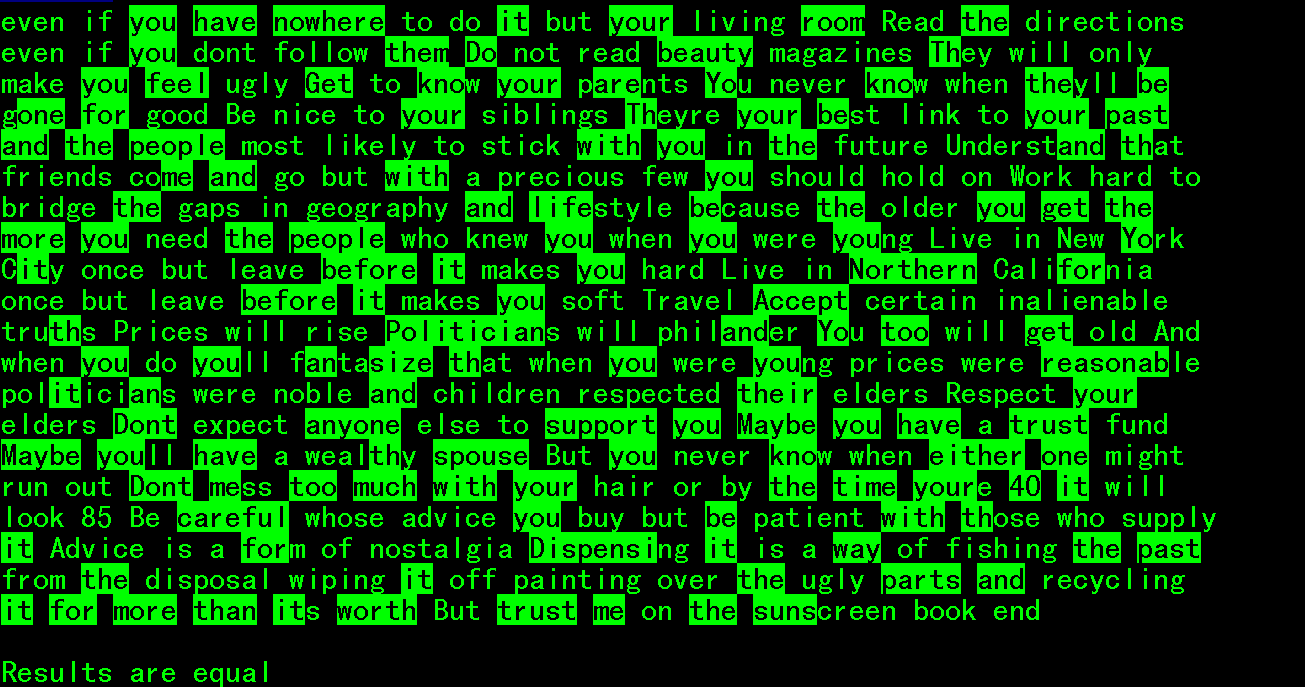
\includegraphics[angle=270,origin=b,width=0.70\textwidth]{string.eps}
\caption{String search}
\end{figure}

\begin{screen}
\tiny
\begin{verbatim}
orig()
{
  int i;
  printf("<<<ORIG>>>\n");
  for (i=0; i<snum; i++) {
    init_search(i);
    strsearch(i);
  }
  return 0;
}
init_search(int i)/* for ARM */
{
  char *str = sstr[i];
  int  len  = slen[i];
  int  j;
  for (j = 0; j <= UCHAR_MAX; j++)
    table[j] = len;
  for (j = 0; j < len; j++)
    table[(Uchar)str[j]] = len - j - 1;
  for (j = 0; j < clen; j++)
    *(out0+clen*i+j) = 0;
}
strsearch(int i)
{
  char *str = sstr[i];
  int  len  = slen[i];
  register size_t shift;
  register size_t pos = len - 1;
  char   *found;
  while (pos < clen) {
    while (pos < clen && (shift = table[(unsigned char)target[pos]]) > 0)
      pos += shift;
    if (!shift) {
      if (!strncmp(str, &target[pos-len+1], len))
        out0[i*clen+(pos-len+1)] = 0xff;
      pos++;
} } }
\end{verbatim}
\end{screen}

\begin{screen}
\tiny
\begin{verbatim}
imax()
{
  int i, j;
  printf("<<<IMAX>>>\n");
  for (i=0; i<snum; i++) {
    for (j=0; j<clen; j++) {
      if (!strncmp(sstr[i], &target[j], slen[i]))
        out1[i*clen+j] = 0xff;
      else
        out1[i*clen+j] = 0;
} } }
\end{verbatim}
\end{screen}

\begin{screen}
\tiny
\begin{verbatim}
imax()
{
  Ull   CHIP;
  Ull   LOOP1, LOOP0;
  Ull   INIT1, INIT0;
  Ull   AR[64][4];                     /* output of EX     in each unit */
  Ull   BR[64][4][4];                  /* output registers in each unit */
  Ull   r00, r01, r02, r03, r04, r05, r06, r07, r08, r09, r10, r11, r12, r13, r14, r15;
  Ull   r16, r17, r18, r19, r20, r21, r22, r23, r24, r25, r26, r27, r28, r29, r30, r31;
  Ull   c0, c1, c2, c3, ex0, ex1;
  Ull   t0[NCHIP], t1[NCHIP], t2[NCHIP], t3[NCHIP], t4[NCHIP], t5[NCHIP], t6[NCHIP], t7[NCHIP], t8[NCHIP];
  Ull   t0t[NCHIP], t1t[NCHIP], t2t[NCHIP], t3t[NCHIP], t4t[NCHIP], t5t[NCHIP], t6t[NCHIP], t7t[NCHIP], t8t[NCHIP];
  Ull   r0[NCHIP], r1[NCHIP], r2[NCHIP], r3[NCHIP], r4[NCHIP], r5[NCHIP], r6[NCHIP], r7[NCHIP], r8[NCHIP];
  Ull   r0t[NCHIP], r1t[NCHIP], r2t[NCHIP], r3t[NCHIP], r4t[NCHIP], r5t[NCHIP], r6t[NCHIP], r7t[NCHIP], r8t[NCHIP];
  Ull   i, dmy, loop=clen/NCHIP;
  Ull   dwi = clen/NCHIP/4+1; /* dwords */
  Ull   dwo = clen/NCHIP/4  ; /* dwords */

  printf("<<<IMAX>>>\n");
  for (CHIP=0; CHIP<NCHIP; CHIP++) {
    t0t[CHIP]=target+(clen/NCHIP*CHIP);
    t1t[CHIP]=target+(clen/NCHIP*CHIP);
    t2t[CHIP]=target+(clen/NCHIP*CHIP);
    t3t[CHIP]=target+(clen/NCHIP*CHIP);
    t4t[CHIP]=target+(clen/NCHIP*CHIP);
    t5t[CHIP]=target+(clen/NCHIP*CHIP);
    t6t[CHIP]=target+(clen/NCHIP*CHIP);
    t7t[CHIP]=target+(clen/NCHIP*CHIP);
    t8t[CHIP]=target+(clen/NCHIP*CHIP);
  }
  for (i=0; i<snum; i+=OMAP) {
    Ull  c00=sstr[i+0][0], c01=sstr[i+0][1], c02=sstr[i+0][2], c03=sstr[i+0][3], c04=sstr[i+0][4], c05=sstr[i+0][5], c06=sstr[i+0][6], c07=sstr[i+0][7];
    Ull  c10=sstr[i+1][0], c11=sstr[i+1][1], c12=sstr[i+1][2], c13=sstr[i+1][3], c14=sstr[i+1][4], c15=sstr[i+1][5], c16=sstr[i+1][6], c17=sstr[i+1][7];
         :
    Ull  c80=sstr[i+8][0], c81=sstr[i+8][1], c82=sstr[i+8][2], c83=sstr[i+8][3], c84=sstr[i+8][4], c85=sstr[i+8][5], c86=sstr[i+8][6], c87=sstr[i+8][7];
    Ull  slen0=slen[i+0], slen1=slen[i+1], slen2=slen[i+2], slen3=slen[i+3], slen4=slen[i+4], slen5=slen[i+5], slen6=slen[i+6], slen7=slen[i+7], slen8=slen[i+8];
    for (CHIP=0; CHIP<NCHIP; CHIP++) {
      t0[CHIP] = t0t[CHIP]-1;
      t1[CHIP] = t1t[CHIP]-1;
        :
      t8[CHIP] = t8t[CHIP]-1;
      r0[CHIP] = r0t[CHIP] = out1+(i+0)*clen+(clen/NCHIP*CHIP);
      r1[CHIP] = r1t[CHIP] = out1+(i+1)*clen+(clen/NCHIP*CHIP);
        :
      r8[CHIP] = r8t[CHIP] = out1+(i+8)*clen+(clen/NCHIP*CHIP);
    }
//EMAX5A begin search mapdist=0
    for (CHIP=0; CHIP<NCHIP; CHIP++) { //���å������ϸ����о�ʸ����礭������
      for (INIT0=1,LOOP0=loop,dmy=0; LOOP0--; INIT0=0) { //Ĺ����64KBʸ���ޤ�
      /* map#0 */
/*@0,1*/ exe(OP_ADD,       &t0[CHIP],     t0[CHIP], EXP_H3210,   1LL,          EXP_H3210, 0LL, EXP_H3210, OP_AND, 0x00000000ffffffffLL, OP_NOP, 0LL);
/*@1,0*/ exe(OP_MCAS,      &r00,          slen0,    EXP_H3210,   1,            EXP_H3210, 0LL, EXP_H3210, OP_NOP, 0LL,    OP_NOP,  0LL);
/*@1,1*/ exe(OP_MCAS,      &r01,          slen0,    EXP_H3210,   2,            EXP_H3210, 0LL, EXP_H3210, OP_NOP, 0LL,    OP_NOP,  0LL);
/*@1,2*/ exe(OP_MCAS,      &r02,          slen0,    EXP_H3210,   3,            EXP_H3210, 0LL, EXP_H3210, OP_NOP, 0LL,    OP_NOP,  0LL);
/*@1,3*/ exe(OP_MCAS,      &r03,          slen0,    EXP_H3210,   4,            EXP_H3210, 0LL, EXP_H3210, OP_NOP, 0LL,    OP_NOP,  0LL);
/*@1,0*/ mop(OP_LDBR,  1,  &BR[1][0][1],  t0[CHIP], 0,   MSK_D0, t0t[CHIP],    dwi,  0,   0,   (Ull)NULL,  dwi);
/*@1,0*/ mop(OP_LDBR,  1,  &BR[1][0][0],  t0[CHIP], 1,   MSK_D0, t0t[CHIP],    dwi,  0,   0,   (Ull)NULL,  dwi);
/*@1,1*/ mop(OP_LDBR,  1,  &BR[1][1][1],  t0[CHIP], 2,   MSK_D0, t0t[CHIP],    dwi,  0,   0,   (Ull)NULL,  dwi);
/*@1,1*/ mop(OP_LDBR,  1,  &BR[1][1][0],  t0[CHIP], 3,   MSK_D0, t0t[CHIP],    dwi,  0,   0,   (Ull)NULL,  dwi);
/*@1,2*/ mop(OP_LDBR,  1,  &BR[1][2][1],  t0[CHIP], 4,   MSK_D0, t0t[CHIP],    dwi,  0,   0,   (Ull)NULL,  dwi);
/*@1,2*/ mop(OP_LDBR,  1,  &BR[1][2][0],  t0[CHIP], 5,   MSK_D0, t0t[CHIP],    dwi,  0,   0,   (Ull)NULL,  dwi);
/*@1,3*/ mop(OP_LDBR,  1,  &BR[1][3][1],  t0[CHIP], 6,   MSK_D0, t0t[CHIP],    dwi,  0,   0,   (Ull)NULL,  dwi);
/*@1,3*/ mop(OP_LDBR,  1,  &BR[1][3][0],  t0[CHIP], 7,   MSK_D0, t0t[CHIP],    dwi,  0,   0,   (Ull)NULL,  dwi);
/*@2,0*/ exe(OP_CMP_NE,    &r16,          c00,      EXP_H3210,   BR[1][0][1],  EXP_H3210, 0LL, EXP_H3210, OP_AND, r00,    OP_NOP,  0LL); // 1 if unmatch
/*@2,1*/ exe(OP_CMP_NE,    &r17,          c01,      EXP_H3210,   BR[1][0][0],  EXP_H3210, 0LL, EXP_H3210, OP_AND, r01,    OP_NOP,  0LL); // 1 if unmatch
/*@2,2*/ exe(OP_CMP_NE,    &r18,          c02,      EXP_H3210,   BR[1][1][1],  EXP_H3210, 0LL, EXP_H3210, OP_AND, r02,    OP_NOP,  0LL); // 1 if unmatch
/*@2,3*/ exe(OP_CMP_NE,    &r19,          c03,      EXP_H3210,   BR[1][1][0],  EXP_H3210, 0LL, EXP_H3210, OP_AND, r03,    OP_NOP,  0LL); // 1 if unmatch
/*@3,0*/ exe(OP_MCAS,      &r04,          slen0,    EXP_H3210,   5,            EXP_H3210, 0LL, EXP_H3210, OP_NOP, 0LL,    OP_NOP,  0LL);
/*@3,1*/ exe(OP_MCAS,      &r05,          slen0,    EXP_H3210,   6,            EXP_H3210, 0LL, EXP_H3210, OP_NOP, 0LL,    OP_NOP,  0LL);
/*@3,2*/ exe(OP_MCAS,      &r06,          slen0,    EXP_H3210,   7,            EXP_H3210, 0LL, EXP_H3210, OP_NOP, 0LL,    OP_NOP,  0LL);
/*@3,3*/ exe(OP_MCAS,      &r07,          slen0,    EXP_H3210,   8,            EXP_H3210, 0LL, EXP_H3210, OP_NOP, 0LL,    OP_NOP,  0LL);
/*@4,0*/ exe(OP_CMP_NE,    &r20,          c04,      EXP_H3210,   BR[1][2][1],  EXP_H3210, 0LL, EXP_H3210, OP_AND, r04,    OP_NOP,  0LL); // 1 if unmatch
/*@4,1*/ exe(OP_CMP_NE,    &r21,          c05,      EXP_H3210,   BR[1][2][0],  EXP_H3210, 0LL, EXP_H3210, OP_AND, r05,    OP_NOP,  0LL); // 1 if unmatch
/*@4,2*/ exe(OP_CMP_NE,    &r22,          c06,      EXP_H3210,   BR[1][3][1],  EXP_H3210, 0LL, EXP_H3210, OP_AND, r06,    OP_NOP,  0LL); // 1 if unmatch
/*@4,3*/ exe(OP_CMP_NE,    &r23,          c07,      EXP_H3210,   BR[1][3][0],  EXP_H3210, 0LL, EXP_H3210, OP_AND, r07,    OP_NOP,  0LL); // 1 if unmatch
/*@5,0*/ exe(OP_ADD3,      &r10,          r16,      EXP_H3210,   r17,          EXP_H3210, r18, EXP_H3210, OP_NOP, 0LL,    OP_NOP,  0LL); //
/*@5,1*/ exe(OP_ADD3,      &r11,          r19,      EXP_H3210,   r20,          EXP_H3210, r21, EXP_H3210, OP_NOP, 0LL,    OP_NOP,  0LL); //
/*@5,2*/ exe(OP_ADD,       &r12,          r22,      EXP_H3210,   r23,          EXP_H3210, 0LL, EXP_H3210, OP_NOP, 0LL,    OP_NOP,  0LL); //
/*@6,0*/ exe(OP_ADD3,      &r00,          r10,      EXP_H3210,   r11,          EXP_H3210, r12, EXP_H3210, OP_NOP, 0LL,    OP_NOP,  0LL); //
/*@7,0*/ exe(OP_MCAS,      &r31,          0LL,      EXP_H3210,   r00,          EXP_H3210, 0LL, EXP_H3210, OP_NOP, 0LL,    OP_NOP,  0LL); // FF if match
/*@7,0*/ mop(OP_STBR, 3,   &r31,          r0[CHIP]++, 0, MSK_D0, r0t[CHIP],    dwo,  0,   0,   (Ull)NULL,  dwo);
        :
      /* map#8 */
/*@56,1*/exe(OP_ADD,       &t8[CHIP],     t8[CHIP], EXP_H3210,   1LL,          EXP_H3210, 0LL, EXP_H3210, OP_AND, 0x00000000ffffffffLL, OP_NOP, 0LL);
/*@57,0*/exe(OP_MCAS,      &r00,          slen8,    EXP_H3210,   1,            EXP_H3210, 0LL, EXP_H3210, OP_NOP, 0LL,    OP_NOP,  0LL);
/*@57,1*/exe(OP_MCAS,      &r01,          slen8,    EXP_H3210,   2,            EXP_H3210, 0LL, EXP_H3210, OP_NOP, 0LL,    OP_NOP,  0LL);
/*@57,2*/exe(OP_MCAS,      &r02,          slen8,    EXP_H3210,   3,            EXP_H3210, 0LL, EXP_H3210, OP_NOP, 0LL,    OP_NOP,  0LL);
/*@57,3*/exe(OP_MCAS,      &r03,          slen8,    EXP_H3210,   4,            EXP_H3210, 0LL, EXP_H3210, OP_NOP, 0LL,    OP_NOP,  0LL);
/*@57,0*/mop(OP_LDBR,  1,  &BR[57][0][1], t8[CHIP], 0,   MSK_D0, t7t[CHIP],    dwi,  0,   0,   (Ull)NULL,  dwi);
/*@57,0*/mop(OP_LDBR,  1,  &BR[57][0][0], t8[CHIP], 1,   MSK_D0, t7t[CHIP],    dwi,  0,   0,   (Ull)NULL,  dwi);
/*@57,1*/mop(OP_LDBR,  1,  &BR[57][1][1], t8[CHIP], 2,   MSK_D0, t7t[CHIP],    dwi,  0,   0,   (Ull)NULL,  dwi);
/*@57,1*/mop(OP_LDBR,  1,  &BR[57][1][0], t8[CHIP], 3,   MSK_D0, t7t[CHIP],    dwi,  0,   0,   (Ull)NULL,  dwi);
/*@57,2*/mop(OP_LDBR,  1,  &BR[57][2][1], t8[CHIP], 4,   MSK_D0, t7t[CHIP],    dwi,  0,   0,   (Ull)NULL,  dwi);
/*@57,2*/mop(OP_LDBR,  1,  &BR[57][2][0], t8[CHIP], 5,   MSK_D0, t7t[CHIP],    dwi,  0,   0,   (Ull)NULL,  dwi);
/*@57,3*/mop(OP_LDBR,  1,  &BR[57][3][1], t8[CHIP], 6,   MSK_D0, t7t[CHIP],    dwi,  0,   0,   (Ull)NULL,  dwi);
/*@57,3*/mop(OP_LDBR,  1,  &BR[57][3][0], t8[CHIP], 7,   MSK_D0, t7t[CHIP],    dwi,  0,   0,   (Ull)NULL,  dwi);
/*@58,0*/exe(OP_CMP_NE,    &r16,          c80,      EXP_H3210,   BR[57][0][1], EXP_H3210, 0LL, EXP_H3210, OP_AND, r00,    OP_NOP,  0LL); // 1 if unmatch
/*@58,1*/exe(OP_CMP_NE,    &r17,          c81,      EXP_H3210,   BR[57][0][0], EXP_H3210, 0LL, EXP_H3210, OP_AND, r01,    OP_NOP,  0LL); // 1 if unmatch
/*@58,2*/exe(OP_CMP_NE,    &r18,          c82,      EXP_H3210,   BR[57][1][1], EXP_H3210, 0LL, EXP_H3210, OP_AND, r02,    OP_NOP,  0LL); // 1 if unmatch
/*@58,3*/exe(OP_CMP_NE,    &r19,          c83,      EXP_H3210,   BR[57][1][0], EXP_H3210, 0LL, EXP_H3210, OP_AND, r03,    OP_NOP,  0LL); // 1 if unmatch
/*@59,0*/exe(OP_MCAS,      &r04,          slen8,    EXP_H3210,   5,            EXP_H3210, 0LL, EXP_H3210, OP_NOP, 0LL,    OP_NOP,  0LL);
/*@59,1*/exe(OP_MCAS,      &r05,          slen8,    EXP_H3210,   6,            EXP_H3210, 0LL, EXP_H3210, OP_NOP, 0LL,    OP_NOP,  0LL);
/*@59,2*/exe(OP_MCAS,      &r06,          slen8,    EXP_H3210,   7,            EXP_H3210, 0LL, EXP_H3210, OP_NOP, 0LL,    OP_NOP,  0LL);
/*@59,3*/exe(OP_MCAS,      &r07,          slen8,    EXP_H3210,   8,            EXP_H3210, 0LL, EXP_H3210, OP_NOP, 0LL,    OP_NOP,  0LL);
/*@60,0*/exe(OP_CMP_NE,    &r20,          c84,      EXP_H3210,   BR[57][2][1], EXP_H3210, 0LL, EXP_H3210, OP_AND, r04,    OP_NOP,  0LL); // 1 if unmatch
/*@60,1*/exe(OP_CMP_NE,    &r21,          c85,      EXP_H3210,   BR[57][2][0], EXP_H3210, 0LL, EXP_H3210, OP_AND, r05,    OP_NOP,  0LL); // 1 if unmatch
/*@60,2*/exe(OP_CMP_NE,    &r22,          c86,      EXP_H3210,   BR[57][3][1], EXP_H3210, 0LL, EXP_H3210, OP_AND, r06,    OP_NOP,  0LL); // 1 if unmatch
/*@60,3*/exe(OP_CMP_NE,    &r23,          c87,      EXP_H3210,   BR[57][3][0], EXP_H3210, 0LL, EXP_H3210, OP_AND, r07,    OP_NOP,  0LL); // 1 if unmatch
/*@61,0*/exe(OP_ADD3,      &r10,          r16,      EXP_H3210,   r17,          EXP_H3210, r18, EXP_H3210, OP_NOP, 0LL,    OP_NOP,  0LL); //
/*@61,1*/exe(OP_ADD3,      &r11,          r19,      EXP_H3210,   r20,          EXP_H3210, r21, EXP_H3210, OP_NOP, 0LL,    OP_NOP,  0LL); //
/*@61,2*/exe(OP_ADD,       &r12,          r22,      EXP_H3210,   r23,          EXP_H3210, 0LL, EXP_H3210, OP_NOP, 0LL,    OP_NOP,  0LL); //
/*@62,0*/exe(OP_ADD3,      &r00,          r10,      EXP_H3210,   r11,          EXP_H3210, r12, EXP_H3210, OP_NOP, 0LL,    OP_NOP,  0LL); //
/*@63,0*/exe(OP_MCAS,      &r31,          0LL,      EXP_H3210,   r00,          EXP_H3210, 0LL, EXP_H3210, OP_NOP, 0LL,    OP_NOP,  0LL); // FF if match
/*@63,0*/mop(OP_STBR, 3,   &r31,          r8[CHIP]++, 0, MSK_D0, r8t[CHIP],    dwo,  0,   0,   (Ull)NULL,  dwo);
      }
    }
//EMAX5A end
//EMAX5A drain_dirty_lmm
  }
}
\end{verbatim}
\end{screen}

\begin{figure}[htbp]
\center
\epsfile{file=pbmsrch+rmm-search-emax6.eps,width=1.00\textwidth}
\caption{String search}
\end{figure}

\clearpage

\subsection{16x16 Convolution}

\shabox{
\leftline{cent\% make -f Makefile-csim.emax6+dma all clean}
\leftline{cent\% ../../src/csim/csim -x conv16-csim.emax6+dma}
}

\shabox{
\leftline{zynq\% make -f Makefile-zynq.emax6+dma all clean}
\leftline{zynq\% ./conv16-zynq.emax6+dma}
}

\vskip .1in

This is a 16x16 convolution operation. Only one row is calculated by one burst operation. This is a stencil calculation and mapdist = 2.

\begin{screen}
\tiny
\begin{verbatim}
conv16_x1(float *yi, float *yo)
{
 Ull  loop = image_WD/2-8;
 Ull  x = 8;
#if !defined(EMAX5) && !defined(EMAX6)
 while (loop--) {
 yo[x]= yim8[x-8]*SCON[  0]+yim8[x-7]*SCON[  1]+yim8[x-6]*SCON[  2]+yim8[x-5]*SCON[  3]+yim8[x-4]*SCON[  4]+yim8[x-3]*SCON[  5]+yim8[x-2]*SCON[  6]+yim8[x-1]*SCON[  7]
      + yim8[x+0]*SCON[  8]+yim8[x+1]*SCON[  9]+yim8[x+2]*SCON[ 10]+yim8[x+3]*SCON[ 11]+yim8[x+4]*SCON[ 12]+yim8[x+5]*SCON[ 13]+yim8[x+6]*SCON[ 14]+yim8[x+7]*SCON[ 15]
      + yim7[x-8]*SCON[ 16]+yim7[x-7]*SCON[ 17]+yim7[x-6]*SCON[ 18]+yim7[x-5]*SCON[ 19]+yim7[x-4]*SCON[ 20]+yim7[x-3]*SCON[ 21]+yim7[x-2]*SCON[ 22]+yim7[x-1]*SCON[ 23]
      + yim7[x+0]*SCON[ 24]+yim7[x+1]*SCON[ 25]+yim7[x+2]*SCON[ 26]+yim7[x+3]*SCON[ 27]+yim7[x+4]*SCON[ 28]+yim7[x+5]*SCON[ 29]+yim7[x+6]*SCON[ 30]+yim7[x+7]*SCON[ 31]
      + yim6[x-8]*SCON[ 32]+yim6[x-7]*SCON[ 33]+yim6[x-6]*SCON[ 34]+yim6[x-5]*SCON[ 35]+yim6[x-4]*SCON[ 36]+yim6[x-3]*SCON[ 37]+yim6[x-2]*SCON[ 38]+yim6[x-1]*SCON[ 39]
      :
      + yip1[x+0]*SCON[152]+yip1[x+1]*SCON[153]+yip1[x+2]*SCON[154]+yip1[x+3]*SCON[155]+yip1[x+4]*SCON[156]+yip1[x+5]*SCON[157]+yip1[x+6]*SCON[158]+yip1[x+7]*SCON[159]
      + yip2[x-8]*SCON[160]+yip2[x-7]*SCON[161]+yip2[x-6]*SCON[162]+yip2[x-5]*SCON[163]+yip2[x-4]*SCON[164]+yip2[x-3]*SCON[165]+yip2[x-2]*SCON[166]+yip2[x-1]*SCON[167]
      + yip2[x+0]*SCON[168]+yip2[x+1]*SCON[169]+yip2[x+2]*SCON[170]+yip2[x+3]*SCON[171]+yip2[x+4]*SCON[172]+yip2[x+5]*SCON[173]+yip2[x+6]*SCON[174]+yip2[x+7]*SCON[175]
      + yip3[x-8]*SCON[176]+yip3[x-7]*SCON[177]+yip3[x-6]*SCON[178]+yip3[x-5]*SCON[179]+yip3[x-4]*SCON[180]+yip3[x-3]*SCON[181]+yip3[x-2]*SCON[182]+yip3[x-1]*SCON[183]
      + yip3[x+0]*SCON[184]+yip3[x+1]*SCON[185]+yip3[x+2]*SCON[186]+yip3[x+3]*SCON[187]+yip3[x+4]*SCON[188]+yip3[x+5]*SCON[189]+yip3[x+6]*SCON[190]+yip3[x+7]*SCON[191]
      + yip4[x-8]*SCON[192]+yip4[x-7]*SCON[193]+yip4[x-6]*SCON[194]+yip4[x-5]*SCON[195]+yip4[x-4]*SCON[196]+yip4[x-3]*SCON[197]+yip4[x-2]*SCON[198]+yip4[x-1]*SCON[199]
      + yip4[x+0]*SCON[200]+yip4[x+1]*SCON[201]+yip4[x+2]*SCON[202]+yip4[x+3]*SCON[203]+yip4[x+4]*SCON[204]+yip4[x+5]*SCON[205]+yip4[x+6]*SCON[206]+yip4[x+7]*SCON[207]
      + yip5[x-8]*SCON[208]+yip5[x-7]*SCON[209]+yip5[x-6]*SCON[210]+yip5[x-5]*SCON[211]+yip5[x-4]*SCON[212]+yip5[x-3]*SCON[213]+yip5[x-2]*SCON[214]+yip5[x-1]*SCON[215]
      + yip5[x+0]*SCON[216]+yip5[x+1]*SCON[217]+yip5[x+2]*SCON[218]+yip5[x+3]*SCON[219]+yip5[x+4]*SCON[220]+yip5[x+5]*SCON[221]+yip5[x+6]*SCON[222]+yip5[x+7]*SCON[223]
      + yip6[x-8]*SCON[224]+yip6[x-7]*SCON[225]+yip6[x-6]*SCON[226]+yip6[x-5]*SCON[227]+yip6[x-4]*SCON[228]+yip6[x-3]*SCON[229]+yip6[x-2]*SCON[230]+yip6[x-1]*SCON[231]
      + yip6[x+0]*SCON[232]+yip6[x+1]*SCON[233]+yip6[x+2]*SCON[234]+yip6[x+3]*SCON[235]+yip6[x+4]*SCON[236]+yip6[x+5]*SCON[237]+yip6[x+6]*SCON[238]+yip6[x+7]*SCON[239]
      + yip7[x-8]*SCON[240]+yip7[x-7]*SCON[241]+yip7[x-6]*SCON[242]+yip7[x-5]*SCON[243]+yip7[x-4]*SCON[244]+yip7[x-3]*SCON[245]+yip7[x-2]*SCON[246]+yip7[x-1]*SCON[247]
      + yip7[x+0]*SCON[248]+yip7[x+1]*SCON[249]+yip7[x+2]*SCON[250]+yip7[x+3]*SCON[251]+yip7[x+4]*SCON[252]+yip7[x+5]*SCON[253]+yip7[x+6]*SCON[254]+yip7[x+7]*SCON[255];
 x += 2;
 }
#endif
\end{verbatim}
\end{screen}

\begin{screen}
\tiny
\begin{verbatim}
  Ull  AR[64][4];                     /* output of EX     in each unit */
  Ull  BR[64][4][4];                  /* output registers in each unit */
  Ull  r0, r1, r2, r3, r4, r5, r6, r7, r8, r9, r10, r11, r12, r13, r14, r15;
  Ull  r16, r17, r18, r19, r20, r21, r22, r23, r24, r25, r26, r27, r28, r29, r30, r31;
  Ull c000=DCON[  0], c002=DCON[  1], c004=DCON[  2], c006=DCON[  3], c008=DCON[  4], c010=DCON[  5], c012=DCON[  6], c014=DCON[  7];
  Ull c016=DCON[  8], c018=DCON[  9], c020=DCON[ 10], c022=DCON[ 11], c024=DCON[ 12], c026=DCON[ 13], c028=DCON[ 14], c030=DCON[ 15];
  Ull c032=DCON[ 16], c034=DCON[ 17], c036=DCON[ 18], c038=DCON[ 19], c040=DCON[ 20], c042=DCON[ 21], c044=DCON[ 22], c046=DCON[ 23];
  Ull c048=DCON[ 24], c050=DCON[ 25], c052=DCON[ 26], c054=DCON[ 27], c056=DCON[ 28], c058=DCON[ 29], c060=DCON[ 30], c062=DCON[ 31];
  Ull c064=DCON[ 32], c066=DCON[ 33], c068=DCON[ 34], c070=DCON[ 35], c072=DCON[ 36], c074=DCON[ 37], c076=DCON[ 38], c078=DCON[ 39];
       :
  Ull c240=DCON[120], c242=DCON[121], c244=DCON[122], c246=DCON[123], c248=DCON[124], c250=DCON[125], c252=DCON[126], c254=DCON[127];
//EMAX5A begin x1 mapdist=2
  while (loop--) {                                  /* mapped to WHILE() on BR[15][0][0] stage#0 */
    mop(OP_LDR,  3, &BR[0][0][1], yim80++, 0, MSK_D0, yim80, 320, 0, 0, (Ull)NULL, 320); /* stage#0 */
    mop(OP_LDR,  3, &r1,          yim81++, 0, MSK_D0, yim80, 320, 0, 0, (Ull)NULL, 320); /* stage#0 */
    mop(OP_LDR,  3, &r2,          yim82++, 0, MSK_D0, yim80, 320, 0, 0, (Ull)NULL, 320); /* stage#0 */
    mop(OP_LDR,  3, &r3,          yim83++, 0, MSK_D0, yim80, 320, 0, 0, (Ull)NULL, 320); /* stage#0 */
    mop(OP_LDR,  3, &r4,          yim84++, 0, MSK_D0, yim80, 320, 0, 0, (Ull)NULL, 320); /* stage#0 */
    mop(OP_LDR,  3, &r5,          yim85++, 0, MSK_D0, yim80, 320, 0, 0, (Ull)NULL, 320); /* stage#0 */
    mop(OP_LDR,  3, &r6,          yim86++, 0, MSK_D0, yim80, 320, 0, 0, (Ull)NULL, 320); /* stage#0 */
    mop(OP_LDR,  3, &r7,          yim87++, 0, MSK_D0, yim80, 320, 0, 0, (Ull)NULL, 320); /* stage#0 */
    exe(OP_FMA, &r10, 0LL, EXP_H3210, BR[0][0][1], EXP_H3210, c000, EXP_H3210, OP_NOP, 0LL, OP_NOP, 0LL); /* stage#1 */
    exe(OP_FMA, &r11, 0LL, EXP_H3210, r1,          EXP_H3210, c002, EXP_H3210, OP_NOP, 0LL, OP_NOP, 0LL); /* stage#1 */
    exe(OP_FMA, &r12, 0LL, EXP_H3210, r2,          EXP_H3210, c004, EXP_H3210, OP_NOP, 0LL, OP_NOP, 0LL); /* stage#1 */
    exe(OP_FMA, &r13, 0LL, EXP_H3210, r3,          EXP_H3210, c006, EXP_H3210, OP_NOP, 0LL, OP_NOP, 0LL); /* stage#1 */
    exe(OP_FMA, &r20, r10, EXP_H3210, r4,          EXP_H3210, c008, EXP_H3210, OP_NOP, 0LL, OP_NOP, 0LL); /* stage#2 */
    exe(OP_FMA, &r21, r11, EXP_H3210, r5,          EXP_H3210, c010, EXP_H3210, OP_NOP, 0LL, OP_NOP, 0LL); /* stage#2 */
    exe(OP_FMA, &r22, r12, EXP_H3210, r6,          EXP_H3210, c012, EXP_H3210, OP_NOP, 0LL, OP_NOP, 0LL); /* stage#2 */
    exe(OP_FMA, &r23, r13, EXP_H3210, r7,          EXP_H3210, c014, EXP_H3210, OP_NOP, 0LL, OP_NOP, 0LL); /* stage#2 */
    mop(OP_LDR,  3, &BR[2][0][1], yim70++, 0, MSK_D0, yim70, 320, 0, 0, (Ull)NULL, 320); /* stage#2 */
    mop(OP_LDR,  3, &r1,          yim71++, 0, MSK_D0, yim70, 320, 0, 0, (Ull)NULL, 320); /* stage#2 */
    mop(OP_LDR,  3, &r2,          yim72++, 0, MSK_D0, yim70, 320, 0, 0, (Ull)NULL, 320); /* stage#2 */
    mop(OP_LDR,  3, &r3,          yim73++, 0, MSK_D0, yim70, 320, 0, 0, (Ull)NULL, 320); /* stage#2 */
    mop(OP_LDR,  3, &r4,          yim74++, 0, MSK_D0, yim70, 320, 0, 0, (Ull)NULL, 320); /* stage#2 */
    mop(OP_LDR,  3, &r5,          yim75++, 0, MSK_D0, yim70, 320, 0, 0, (Ull)NULL, 320); /* stage#2 */
    mop(OP_LDR,  3, &r6,          yim76++, 0, MSK_D0, yim70, 320, 0, 0, (Ull)NULL, 320); /* stage#2 */
    mop(OP_LDR,  3, &r7,          yim77++, 0, MSK_D0, yim70, 320, 0, 0, (Ull)NULL, 320); /* stage#2 */
        :
    exe(OP_FMA, &r10, r20, EXP_H3210, BR[30][0][1],EXP_H3210, c240, EXP_H3210, OP_NOP, 0LL, OP_NOP, 0LL); /* stage#31 */
    exe(OP_FMA, &r11, r21, EXP_H3210, r1,          EXP_H3210, c242, EXP_H3210, OP_NOP, 0LL, OP_NOP, 0LL); /* stage#31 */
    exe(OP_FMA, &r12, r22, EXP_H3210, r2,          EXP_H3210, c244, EXP_H3210, OP_NOP, 0LL, OP_NOP, 0LL); /* stage#31 */
    exe(OP_FMA, &r13, r23, EXP_H3210, r3,          EXP_H3210, c246, EXP_H3210, OP_NOP, 0LL, OP_NOP, 0LL); /* stage#31 */
    exe(OP_FMA, &r20, r10, EXP_H3210, r4,          EXP_H3210, c248, EXP_H3210, OP_NOP, 0LL, OP_NOP, 0LL); /* stage#32 */
    exe(OP_FMA, &r21, r11, EXP_H3210, r5,          EXP_H3210, c250, EXP_H3210, OP_NOP, 0LL, OP_NOP, 0LL); /* stage#32 */
    exe(OP_FMA, &r22, r12, EXP_H3210, r6,          EXP_H3210, c252, EXP_H3210, OP_NOP, 0LL, OP_NOP, 0LL); /* stage#32 */
    exe(OP_FMA, &r23, r13, EXP_H3210, r7,          EXP_H3210, c254, EXP_H3210, OP_NOP, 0LL, OP_NOP, 0LL); /* stage#32 */

    exe(OP_FAD, &r10,  r20, EXP_H3210,  r21, EXP_H3210, 0LL, EXP_H3210, OP_NOP, 0LL, OP_NOP, 0LL);        /* stage#33 */
    exe(OP_FAD, &r12,  r22, EXP_H3210,  r23, EXP_H3210, 0LL, EXP_H3210, OP_NOP, 0LL, OP_NOP, 0LL);        /* stage#33 */
    exe(OP_FAD, &AR[35][0],  r10, EXP_H3210,  r12, EXP_H3210, 0LL, EXP_H3210, OP_NOP, 0LL, OP_NOP, 0LL);  /* stage#35 */
    mop(OP_STR, 3, &AR[35][0], yoo++, 0LL, MSK_D0, (Ull)yoo, 152, 0, 0, yop, 152);                        /* stage#35 */
  }
//EMAX5A end
#endif
}
\end{verbatim}
\end{screen}

\begin{figure}[htbp]
\center
\epsfile{file=conv16-x1-emax6.eps,width=1.00\textwidth}
\caption{16x16 Convolution}
\end{figure}

\clearpage

\subsection{VBGMM\_Logsum}

\shabox{
\leftline{cent\% make -f Makefile-csim.emax6+dma test016-csim.emax6+dma clean}
\leftline{cent\% ../../src/csim/csim -x test016-csim.emax6+dma}
}

\shabox{
\leftline{zynq\% make -f Makefile-zynq.emax6+dma test016-zynq.emax6+dma clean}
\leftline{zynq\% ./test016-zynq.emax6+dma}
}

\begin{screen}
\tiny
\begin{verbatim}
  for (chip=0; chip<NCHIP; chip++) { /* will be parallelized by multi-chip (M/#chip) */
    for (grp=M/NCHIP*chip; grp<M/NCHIP*(chip+1); grp+=RMGRP) { /* will be parallelized by multi-chip (M/#chip) */
      typedef struct {Uint i[4]} Ui4;
      Ui4  *c60 = C1+grp*M, *c600 = c60;
      Ull  row, bofs, rofs;
      Ull  b00;
      Ull  PARAM = 0x0000000100000001LL; /* 1 */
//EMAX5A begin x1 mapdist=0
/*2*/ for (INIT1=1,LOOP1=RMGRP,row=0-M*4; LOOP1--; INIT1=0) {                                                               /* stage#0 */
  /*1*/ for (INIT0=1,LOOP0=M/W,bofs=0-W*4; LOOP0--; INIT0=0) {                                                              /* stage#0 */
          exe(OP_ADD,    &bofs, INIT0?bofs:bofs, EXP_H3210, W*4, EXP_H3210, 0LL, EXP_H3210, OP_AND, 0x00000000ffffffffLL, OP_NOP, 0LL);/* stage#0 */
          exe(OP_ADD,    &row, row, EXP_H3210, INIT0?M*4:0, EXP_H3210, 0LL, EXP_H3210, OP_NOP, 0LL, OP_NOP, 0LL);           /* stage#0 */
          exe(OP_ADD,    &rofs, row, EXP_H3210, 0LL,  EXP_H3210, 0LL, EXP_H3210, OP_AND, 0x00000000ffffffffLL, OP_NOP, 0LL);/* stage#1 */

          mop(OP_LDWR,   1, &b00,  (Ull)c600, (Ull)rofs,  MSK_W0, (Ull)c60,  M*RMGRP, 0, 1, (Ull)NULL, M*RMGRP);            /* stage#2 */
          exe(OP_ADD,       &b00,  INIT0?b00:b00,   EXP_H3210,  PARAM,  EXP_H3210, 0LL,    EXP_H3210, OP_NOP, 0LL, OP_NOP, 0LL);  /* stage#2 */
          mop(OP_STWR,   1, &b00,  (Ull)rofs, (Ull)c600,  MSK_D0, (Ull)c60,  M*RMGRP, 0, 1, (Ull)NULL, M*RMGRP);            /* stage#2 */
        }
      }
//EMAX5A end
//EMAX5A drain_dirty_lmm
    }
  }
\end{verbatim}
\end{screen}

\clearpage

\subsection{Stochastic sgemm00}

\shabox{
\leftline{cent\% make -f Makefile-csim.emax6+dma test021-csim.emax6+dma clean}
\leftline{cent\% ../../src/csim/csim -x test021-csim.emax6+dma}
}

\shabox{
\leftline{zynq\% make -f Makefile-zynq.emax6+dma test021-zynq.emax6+dma clean}
\leftline{zynq\% ./test021-zynq.emax6+dma}
}

\begin{figure}[htbp]
\center
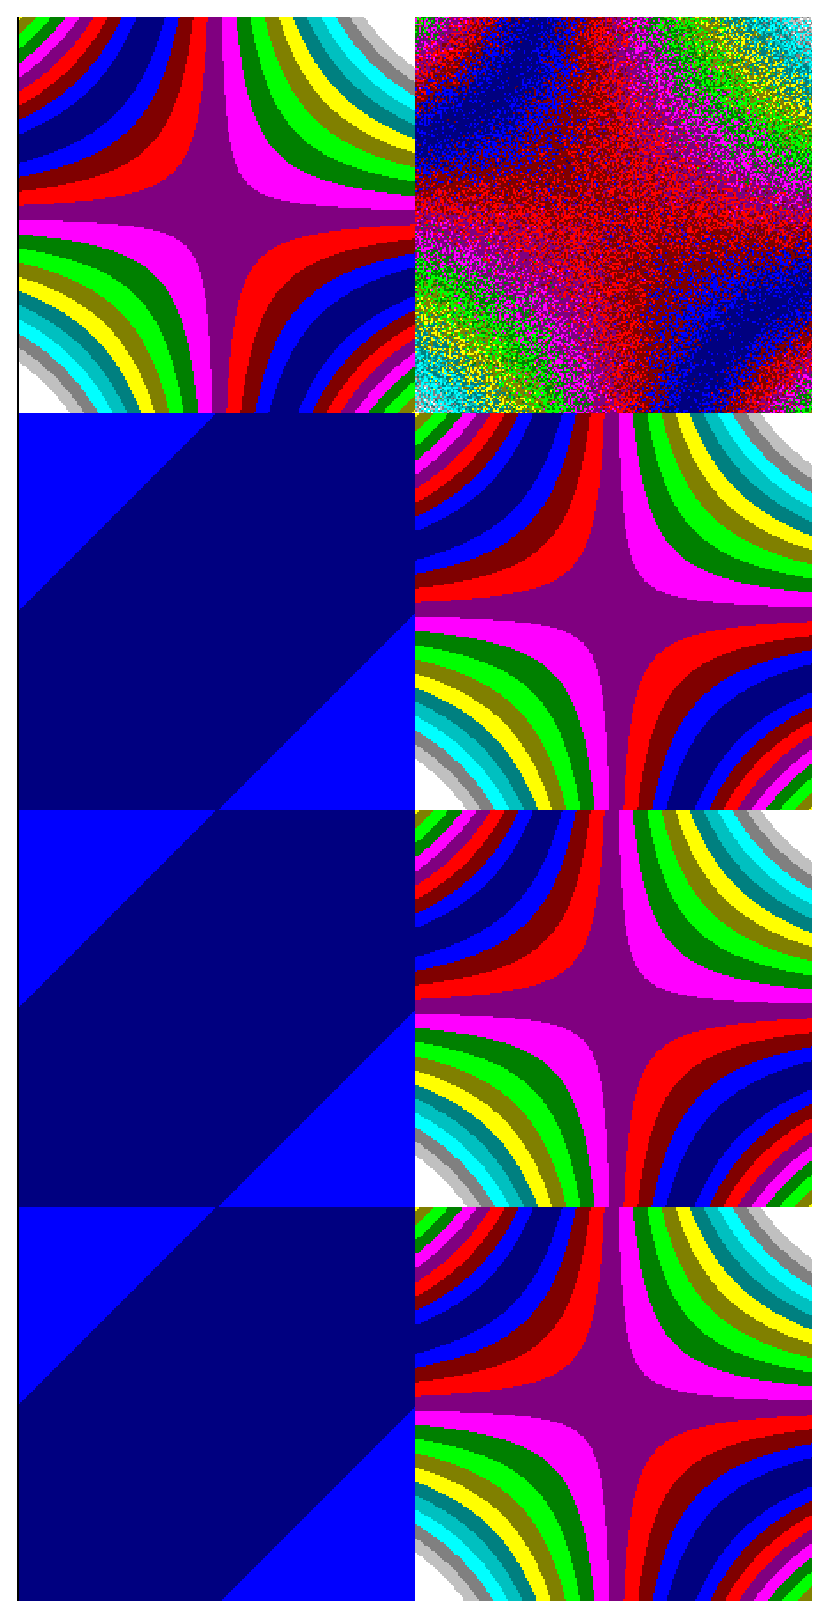
\includegraphics[angle=270,origin=b,width=0.75\textwidth]{stochastic.eps}
\caption{Stochastic sgemm00}
\end{figure}

\begin{screen}
\tiny
\begin{verbatim}
for (top=0; top<BS/NCHIP; top+=H) { /* will be parallelized by multi-chip (M/#chip) */
  for (blk=0; blk<OC4; blk+=RMGRP) { /* 3�ť롼��Ÿ���γ�¦�о� */
    char *a[H][NCHIP];
    char *b, *b0;
    char *c[H][NCHIP], *c0[H][NCHIP];
    b = (Uchar*)i_m0B+blk*IC32; b0 = b+IC32*0;
    for (CHIP=0; CHIP<NCHIP; CHIP++) { /* will be parallelized by multi-chip (M/#chip) */
      for (k=0; k<H; k++) {
        a[k][CHIP] = (Uchar*)i_m0A+(CHIP*BS/NCHIP+top+k)*IC32;
        c[k][CHIP] = (Uchar*)i_m0C+(CHIP*BS/NCHIP+top+k)*OC4+blk;
        c0[k][CHIP]= c[k][CHIP]+0;
      }
    }

#define spike01_core1(r, s) \
  mo4(OP_LDRQ,  1,  BR[r][2], (Ull)b0,                  (Ull)bofs,        MSK_W1,    (Ull)b,          IC32D4RMGRP, 0,      0,   (Ull)NULL, IC32D4RMGRP);/* stage#2 */\
  mo4(OP_LDRQ,  1,  BR[r][1], (Ull)a[s][CHIP],          (Ull)cofs,        MSK_W1,    (Ull)a[s][CHIP], IC32D4,      0,      0,   (Ull)NULL, IC32D4);     /* stage#2 */\
  exe(OP_NOP,      &AR[r][0], 0LL,           EXP_H3210, 0LL,              EXP_H3210, 0LL,             EXP_H3210,   OP_NOP, 0LL, OP_NOP,    0LL);        /* stage#2 */\
  mop(OP_LDBR,  1, &b00,      (Ull)c0[s][CHIP],         (Ull)oofs,        MSK_W0,    (Ull)c[s][CHIP], RMGRPD4,     0,      1,   (Ull)NULL, RMGRPD4);    /* stage#2 */\
  ex4(OP_SFMA,     &b00,      INIT0?b00:b00, EXP_H3210, BR[r][1],         EXP_H3210, BR[r][2],        EXP_H3210,   OP_NOP, 3LL, OP_NOP,    0LL);        /* stage#2 */\
  mop(OP_STBR,  1, &b00,      (Ull)oofs,                (Ull)c0[s][CHIP], MSK_D0,    (Ull)c[s][CHIP], RMGRPD4,     0,      1,   (Ull)NULL, RMGRPD4)     /* stage#2 */

//EMAX5A begin smax2 mapdist=0
/**/for (CHIP=0; CHIP<NCHIP; CHIP++) { /* will be parallelized by multi-chip (M/#chip) */
/*2*/ for (INIT1=1,LOOP1=RMGRP,rofs=(0-IC32)<<32|((0-1LL)&0xffffffff); LOOP1--; INIT1=0) {      /* stage#0 *//* mapped to FOR() on BR[63][1][0] */
  /*1*/ for (INIT0=1,LOOP0=IC32/32,cofs=(0-32LL)<<32|((0)&0xffffffff); LOOP0--; INIT0=0) {      /* stage#0 *//* mapped to FOR() on BR[63][0][0] */
          exe(OP_ADD,    &cofs, INIT0?cofs:cofs, EXP_H3210, (32LL)<<32|(0), EXP_H3210, 0LL, EXP_H3210, OP_AND, 0xffffffffffffffffLL, OP_NOP, 0LL); /* stage#0 */
          exe(OP_ADD,    &rofs, rofs, EXP_H3210, INIT0?IC321:0, EXP_H3210, 0LL, EXP_H3210, OP_NOP, 0LL, OP_NOP, 0LL);  /* stage#0 */
          exe(OP_ADD,    &bofs, rofs, EXP_H3210, cofs, EXP_H3210, 0, EXP_H3210, OP_AND, 0xffffffffffffffffLL, OP_NOP, 0LL);     /* stage#1 */
          exe(OP_ADD,    &oofs, rofs, EXP_H3210, cofs, EXP_H3210, 0, EXP_H3210, OP_AND, 0x00000000ffffffffLL, OP_NOP, 0LL);     /* stage#1 */

          spike01_core1( 2,  0);
          spike01_core1( 3,  1);
          spike01_core1( 4,  2);
          :
          spike01_core1(20, 18);
          spike01_core1(21, 19); /* H=20 */
          spike01_core1(22, 20);
          spike01_core1(23, 21);
          spike01_core1(24, 22);
          spike01_core1(25, 23);
          spike01_core1(26, 24); /* H=25 */
          :
          spike01_core1(50, 48);
          spike01_core1(51, 49); /* H=50 */
        }
      }
    }
//EMAX5A end
  }
}
//EMAX5A drain_dirty_lmm
\end{verbatim}
\end{screen}

\begin{figure}[htbp]
\center
\epsfile{file=smax-smax2-emax6.eps,width=1.00\textwidth}
\caption{Stochastic sgemm00}
\end{figure}

\begin{figure}[htbp]
\center
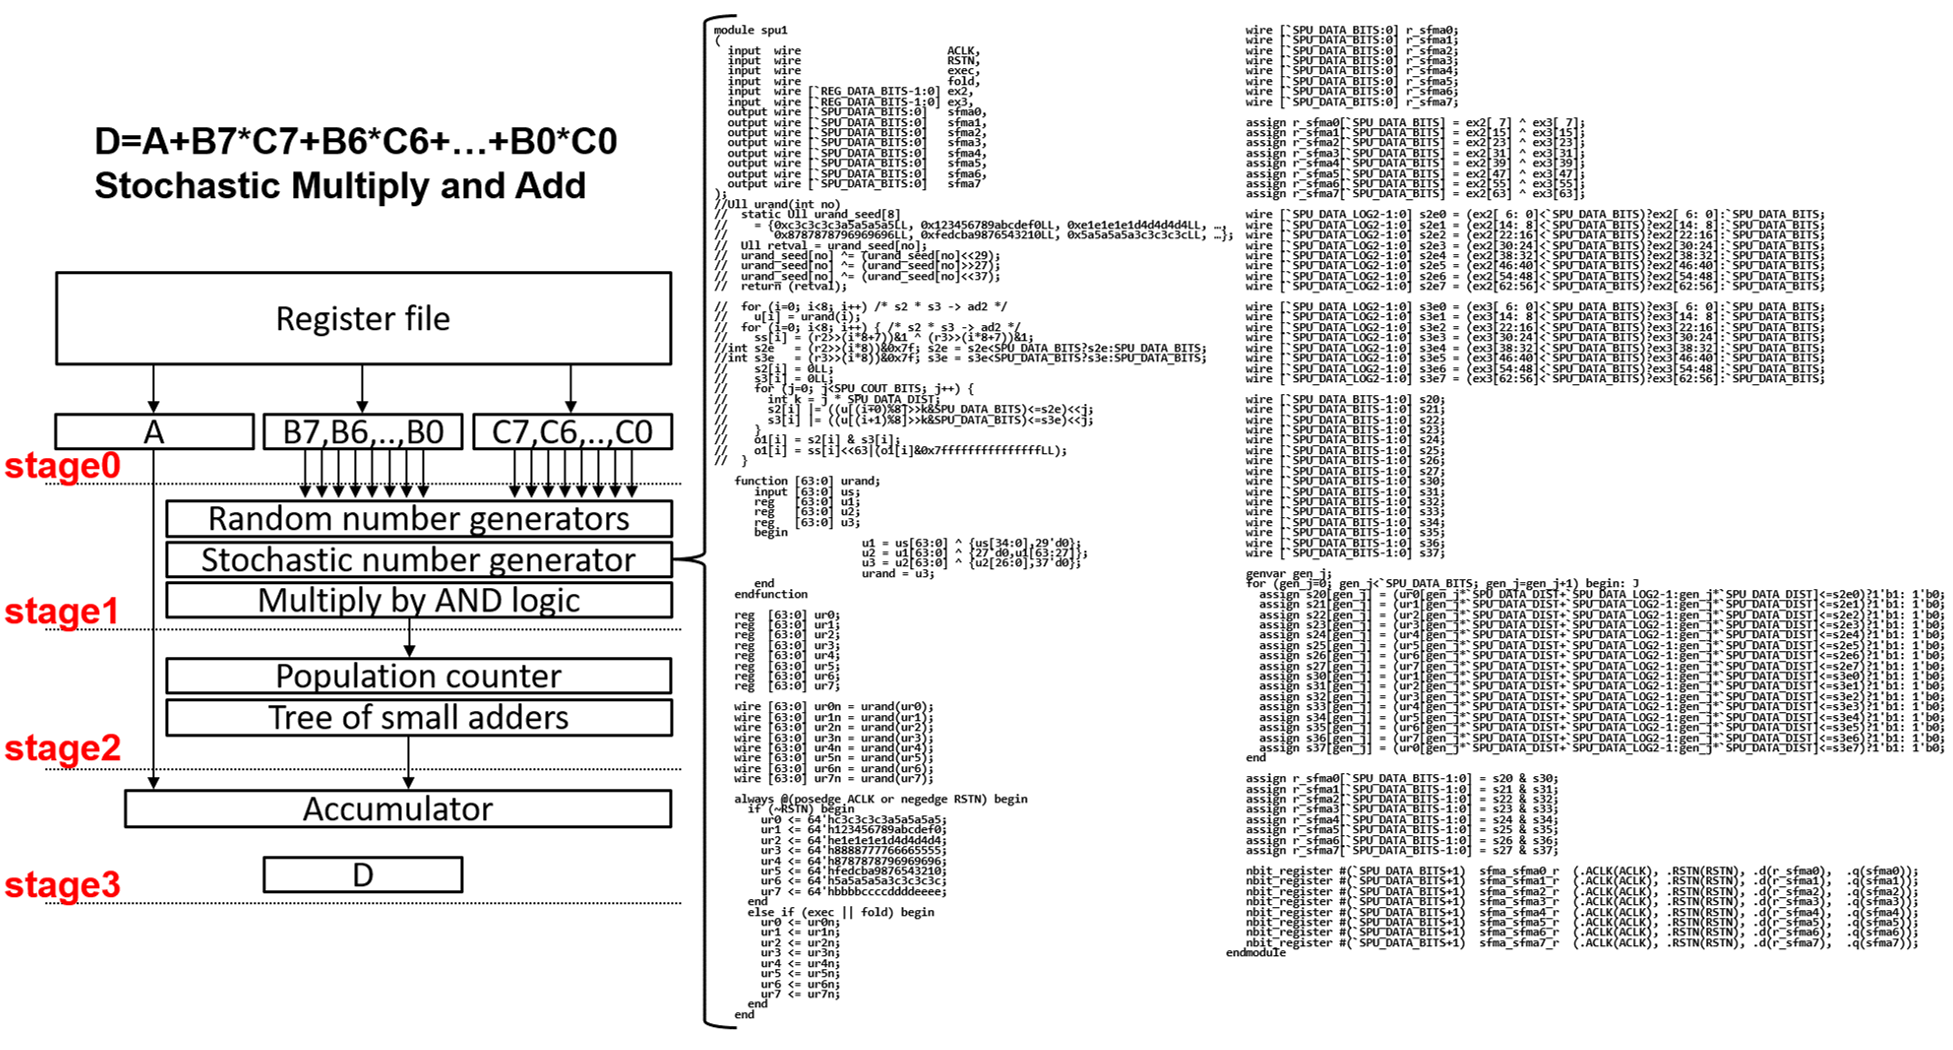
\includegraphics[angle=270,origin=b,width=1.00\textwidth]{sfma1.eps}
\caption{SFMA 1st stage}
\end{figure}

\begin{figure}[htbp]
\center
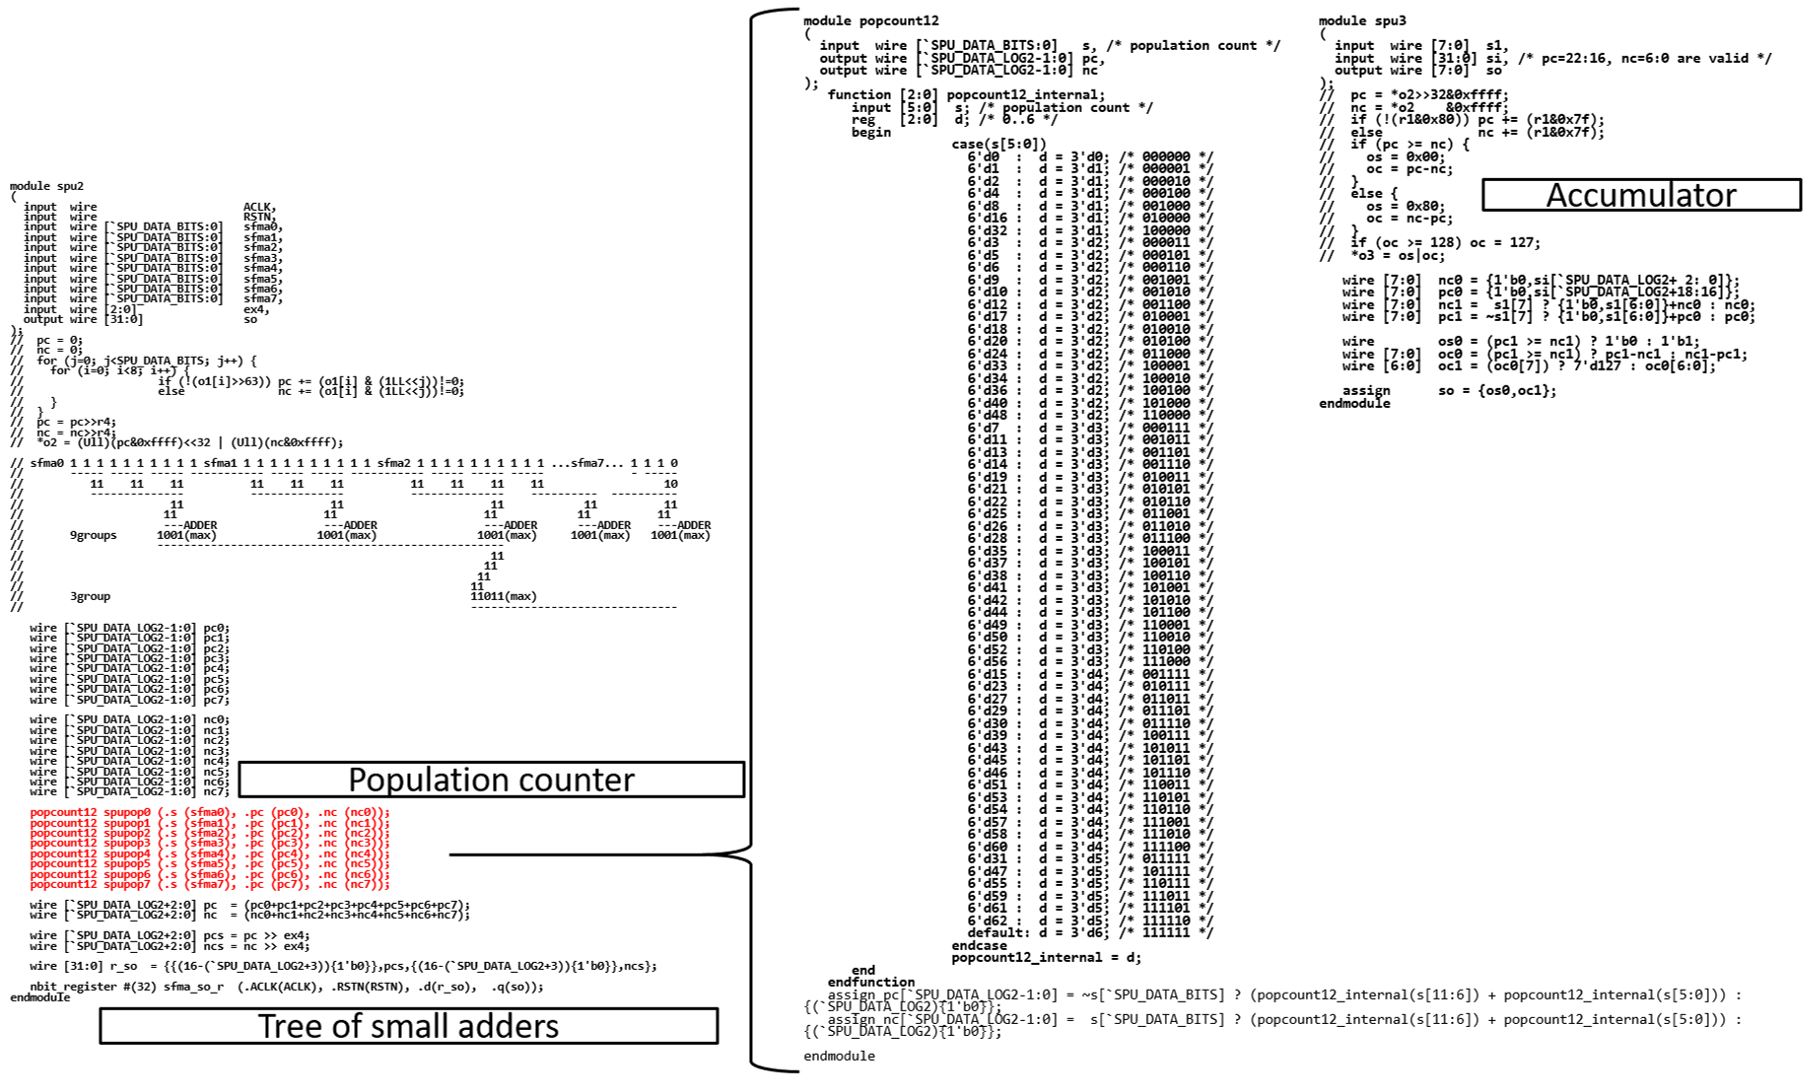
\includegraphics[angle=270,origin=b,width=1.00\textwidth]{sfma2.eps}
\caption{SFMA 2nd and 3rd stage}
\end{figure}

\clearpage

\subsection{Sparse matrix multiplication}

\shabox{
\leftline{cent\% make -f Makefile-csim.emax6+dma test022-csim.emax6+dma clean}
\leftline{cent\% ../../src/csim/csim -x test022-csim.emax6+dma}
}

\shabox{
\leftline{zynq\% make -f Makefile-zynq.emax6+dma test022-zynq.emax6+dma clean}
\leftline{zynq\% ./test022-zynq.emax6+dma}
}

\begin{figure}[htbp]
\center
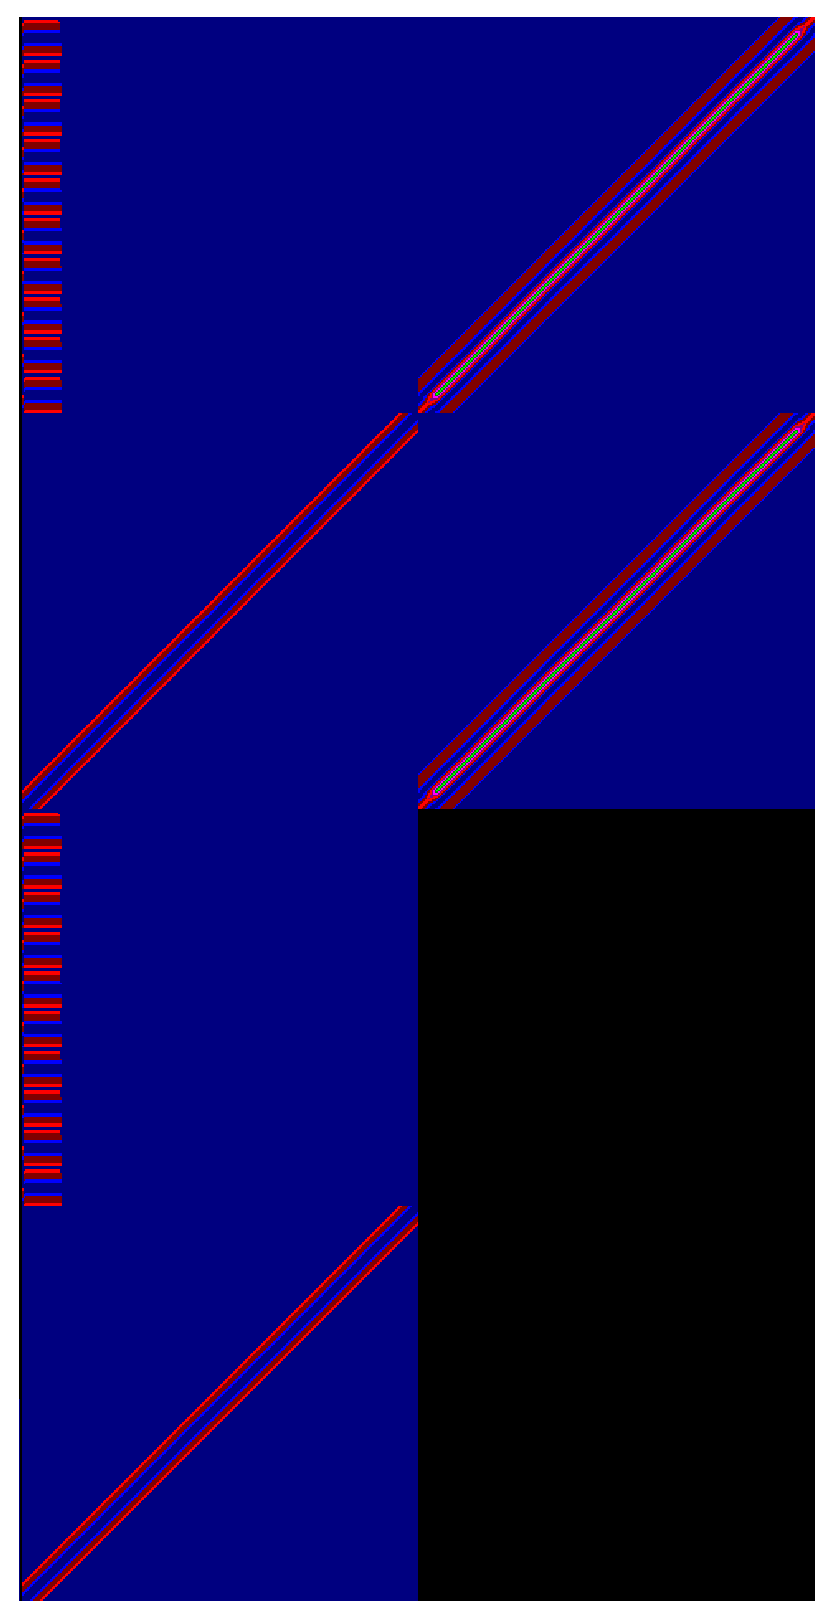
\includegraphics[angle=270,origin=b,width=0.75\textwidth]{sparse_mat.eps}
\caption{Sparse matrix multiplication}
\end{figure}

\subsubsection{Single flow}

\begin{screen}
\tiny
\begin{verbatim}
for (blk=0; blk<M2; blk+=RMGRP) { /* 3�ť롼��Ÿ���γ�¦�о� */
  for (top=0; top<M1/NCHIP; top+=H) { /* will be parallelized by multi-chip (M/#chip) */
    packed *a[H][NCHIP], *a0[H][NCHIP];
    packed *b, *b0[H];
    float  *c[H][NCHIP], *c0[H][NCHIP];
    b = B32_P+blk*LP;
    for (CHIP=0; CHIP<NCHIP; CHIP++) { /* will be parallelized by multi-chip (M/#chip) */
      for (k=0; k<H; k++) {
        a[k][CHIP]  = A32_P+(CHIP*M1/NCHIP+top+k)*LP;
        c[k][CHIP]  = C32_1+(CHIP*M1/NCHIP+top+k)*M2+blk;
        c0[k][CHIP] = c[k][CHIP]+0;
      }
    }

#define sparse_core1(r, h) \
  mex(OP_CMPA_LE,  &b0[h], INIT0?b:b0[h], INIT0?0:8, OP_CMPA_GE, &a0[h][CHIP], INIT0?a[h][CHIP]:a0[h][CHIP], INIT0?0:8, 0LL, BR[r][2][1], BR[r][2][0]);\
  mop(OP_LDR,   3, &BR[r][2][1], b0[h],                        bofs,        MSK_W1,      b,          2*LP*RMGRP,  0, 0,      NULL,      2*LP*RMGRP);/*LMM[2] col2*/\
  mop(OP_LDR,   3, &BR[r][2][0], a0[h][CHIP],                  bofs,        MSK_W0,      a[h][CHIP], 2*LP,        0, 0,      NULL,      2*LP);      /*LMM[1] col2*/\
  exe(OP_NOP,      &AR[r][0],    0LL,                          EXP_H3210,   0,           EXP_H3210,  0,           EXP_H3210, OP_NOP, 0, OP_NOP, 0);\
  mop(OP_LDWR,  1, &c00,         c0[h][CHIP],                  oofs,        MSK_W0,      c[h][CHIP], RMGRP,       0, 1,      NULL,      RMGRP);\
  exe(OP_CFMA,     &c00,         INIT0?c00:c00,                EXP_H3210,   BR[r][2][1], EXP_H3210,  BR[r][2][0], EXP_H3210, OP_NOP, 0, OP_NOP, 0);\
  mop(OP_STWR,  1, &c00,         oofs,                         c0[h][CHIP], MSK_D0,      c[h][CHIP], RMGRP,       0, 1,      NULL,      RMGRP)

//EMAX5A begin imax mapdist=0
/**/for (CHIP=0; CHIP<NCHIP; CHIP++) { /* will be parallelized by multi-chip (M/#chip) */
/*2*/ for (INIT1=1,LOOP1=RMGRP,rofs=(0-LP*8)<<32|((0-4LL)&0xffffffff); LOOP1--; INIT1=0) { /* stage#0 *//* mapped to FOR() on BR[63][1][0] */
  /*1*/ for (INIT0=1,LOOP0=LP,cofs=(0LL)<<32|((0LL)&0xffffffff); LOOP0--; INIT0=0) {         /* stage#0 *//* mapped to FOR() on BR[63][0][0] */
          exe(OP_ADD,    &rofs, rofs, EXP_H3210, INIT0?(LP*8)<<32|(4LL):0, EXP_H3210, 0LL, EXP_H3210, OP_NOP, 0LL,                  OP_NOP, 0LL); /* stage#0 */
          exe(OP_ADD,    &bofs, rofs, EXP_H3210, 0LL,                      EXP_H3210, 0LL, EXP_H3210, OP_AND, 0xffffffff00000000LL, OP_NOP, 0LL); /* stage#1 */
          exe(OP_ADD,    &oofs, rofs, EXP_H3210, 0LL,                      EXP_H3210, 0LL, EXP_H3210, OP_AND, 0x00000000ffffffffLL, OP_NOP, 0LL); /* stage#1 */

          sparse_core1(  2,  0);
          sparse_core1(  3,  1);
          sparse_core1(  4,  2);
          sparse_core1(  5,  3);
          sparse_core1(  6,  4);
          sparse_core1(  7,  5);
          sparse_core1(  8,  6);
          sparse_core1(  9,  7);
          sparse_core1( 10,  8);
          sparse_core1( 11,  9);
          sparse_core1( 12, 10);
          sparse_core1( 13, 11);
          sparse_core1( 14, 12);
          sparse_core1( 15, 13);
          sparse_core1( 16, 14);
          sparse_core1( 17, 15); /* H=16 */
        }
      }
    }
//EMAX5A end
  }
}
//EMAX5A drain_dirty_lmm
\end{verbatim}
\end{screen}

\begin{figure}[htbp]
\center
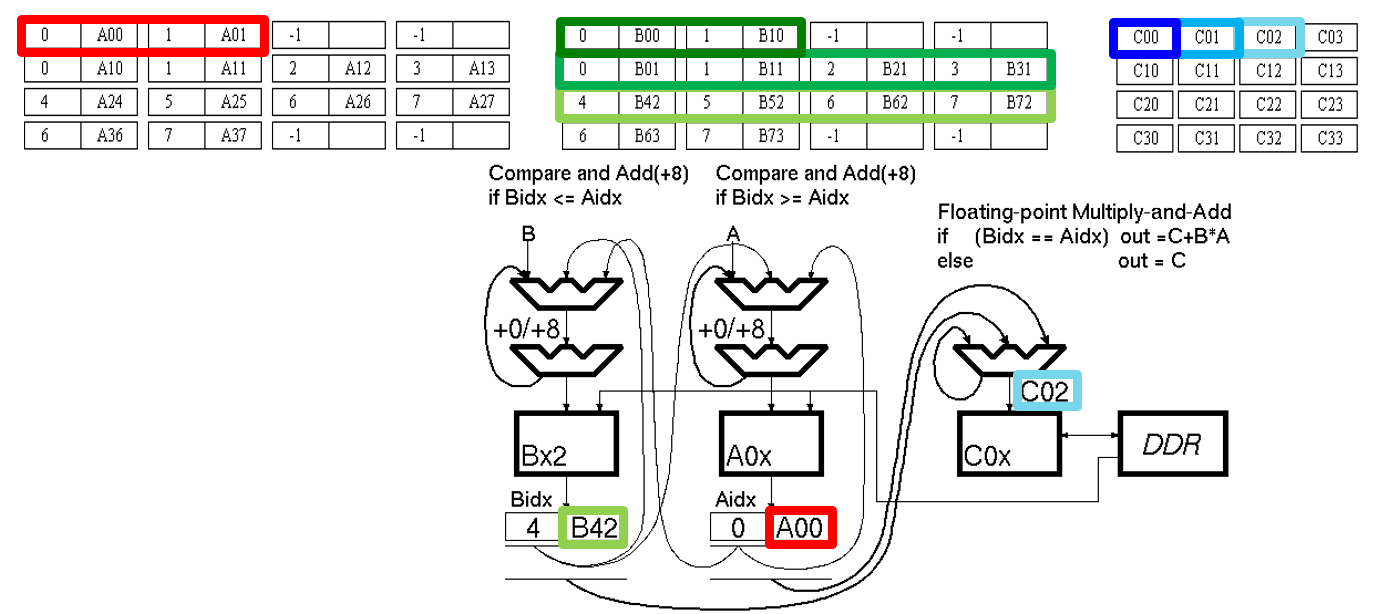
\includegraphics[angle=270,origin=b,width=1.00\textwidth]{SPMM.eps}
\caption{Data path for sparse matrix multiplication}
\end{figure}

\begin{figure}[htbp]
\center
\epsfile{file=EMAX6PIP.eps,width=1.00\textwidth}
\caption{Timing chart (single flow)}
\end{figure}

\begin{figure}[htbp]
\center
\epsfile{file=test022-imax-emax6.eps,width=1.00\textwidth}
\caption{Sparse matrix multiplication (single flow)}
\end{figure}

\clearpage

\subsubsection{Dual flow}

\begin{screen}
\tiny
\begin{verbatim}
  for (blk=0; blk<M2; blk+=RMGRP) { /* 3�ť롼��Ÿ���γ�¦�о� */
    for (top=0; top<M1/NCHIP; top+=H) { /* will be parallelized by multi-chip (M/#chip) */
      packed *a[H][NCHIP], *a0[H][2][NCHIP]; /* a�϶���,a0��Ʊ��Ԥ򻲾�(��ư�ѥ����󤬰㤦�Τ�2��ɬ��) */
      packed *b[2],        *b0[H][2];        /* b�϶���,b0��2�Ԥ�1unit�˥ޥ������åɲ������c��Ϣ³ */
      float  *c[H][NCHIP], *c0[H][2][NCHIP]; /* c�϶���,c0��Ϣ³ */
      b[0] = B32_P+(blk+0)*LP;
      b[1] = B32_P+(blk+1)*LP;
      for (CHIP=0; CHIP<NCHIP; CHIP++) { /* will be parallelized by multi-chip (M/#chip) */
        for (k=0; k<H; k++) {
          a[k][CHIP]  = A32_P+(CHIP*M1/NCHIP+top+k)*LP;
          c[k][CHIP]  = C32_1+(CHIP*M1/NCHIP+top+k)*M2+blk;
          c0[k][0][CHIP] = c[k][CHIP]+0;
          c0[k][1][CHIP] = c[k][CHIP]+1;
      } }
#define sparse_core1(r, h) \
  mex(OP_CMPA_LE, &b0[h][0], INIT0?b[0]:b0[h][0], INIT0?0:8, OP_CMPA_GE, &a0[h][0][CHIP], INIT0?a[h][CHIP]:a0[h][0][CHIP], INIT0?0:8, 0LL, BR[r][2][1], BR[r][2][0]);\
  mop(OP_LDR,   3, &BR[r][2][1],    b0[h][0],                        bofs,           MSK_W1,      b[0],          2*LP*RMGRP,  0, 0,      NULL,      2*LP*RMGRP);\
  mop(OP_LDR,   3, &BR[r][2][0],    a0[h][0][CHIP],                  bofs,           MSK_W0,      a[h][CHIP],    2*LP,        0, 0,      NULL,      2*LP);\
  mex(OP_CMPA_LE, &b0[h][1], INIT0?b[1]:b0[h][1], INIT0?0:8, OP_CMPA_GE, &a0[h][1][CHIP], INIT0?a[h][CHIP]:a0[h][1][CHIP], INIT0?0:8, 0LL, BR[r][3][1], BR[r][3][0]);\
  mop(OP_LDR,   3, &BR[r][3][1],    b0[h][1],                        bofs,           MSK_W1,      b[0],          2*LP*RMGRP,  0, 0,      NULL,      2*LP*RMGRP);\
  mop(OP_LDR,   3, &BR[r][3][0],    a0[h][1][CHIP],                  bofs,           MSK_W0,      a[h][CHIP],    2*LP,        0, 0,      NULL,      2*LP);\
  exe(OP_NOP,      &AR[r][0],       0LL,                             EXP_H3210,      0,           EXP_H3210,     0,           EXP_H3210, OP_NOP, 0, OP_NOP, 0);\
  mop(OP_LDWR,  1, &c00,            c0[h][0][CHIP],                  oofs,           MSK_W0,      c[h][CHIP],    RMGRP,       0, 1,      NULL,      RMGRP);\
  exe(OP_CFMA,     &c00,            INIT0?c00:c00,                   EXP_H3210,      BR[r][2][1], EXP_H3210,     BR[r][2][0], EXP_H3210, OP_NOP, 0, OP_NOP, 0);\
  mop(OP_STWR,  1, &c00,            oofs,                            c0[h][0][CHIP], MSK_D0,      c[h][CHIP],    RMGRP,       0, 1,      NULL,      RMGRP);\
  mop(OP_LDWR,  1, &c01,            c0[h][1][CHIP],                  oofs,           MSK_W0,      c[h][CHIP],    RMGRP,       0, 1,      NULL,      RMGRP);\
  exe(OP_CFMA,     &c01,            INIT0?c01:c01,                   EXP_H3210,      BR[r][3][1], EXP_H3210,     BR[r][3][0], EXP_H3210, OP_NOP, 0, OP_NOP, 0);\
  mop(OP_STWR,  1, &c01,            oofs,                            c0[h][1][CHIP], MSK_D0,      c[h][CHIP],    RMGRP,       0, 1,      NULL,      RMGRP)
//EMAX5A begin imax mapdist=0
/*3*/ for (CHIP=0; CHIP<NCHIP; CHIP++) { /* will be parallelized by multi-chip (M/#chip) */
  /*2*/ for (INIT1=1,LOOP1=RMGRP/2,rofs=(0-8*LP*2)<<32|((0-8LL)&0xffffffff); LOOP1--; INIT1=0) { /* stage#0 *//* mapped to FOR() on BR[63][1][0] */
    /*1*/ for (INIT0=1,LOOP0=LP,cofs=(0LL)<<32|((0LL)&0xffffffff); LOOP0--; INIT0=0) {         /* stage#0 *//* mapped to FOR() on BR[63][0][0] */
            exe(OP_ADD,    &rofs, rofs,            EXP_H3210, INIT0?(8*LP*2)<<32|(8LL):0, EXP_H3210, 0LL, EXP_H3210, OP_NOP, 0LL,                  OP_NOP, 0LL);
            exe(OP_ADD,    &bofs, rofs,            EXP_H3210, 0LL,                        EXP_H3210, 0LL, EXP_H3210, OP_AND, 0xffffffff00000000LL, OP_NOP, 0LL);
            exe(OP_ADD,    &oofs, rofs,            EXP_H3210, 0LL,                        EXP_H3210, 0LL, EXP_H3210, OP_AND, 0x00000000ffffffffLL, OP_NOP, 0LL);
            sparse_core1(  2,  0);
            sparse_core1(  3,  1); /* H=2 */
            sparse_core1(  4,  2);
            sparse_core1(  5,  3); /* H=4 */
            sparse_core1(  6,  4);
            sparse_core1(  7,  5);
            sparse_core1(  8,  6);
            sparse_core1(  9,  7); /* H=8 */
            sparse_core1( 10,  8);
            sparse_core1( 11,  9);
            sparse_core1( 12, 10);
            sparse_core1( 13, 11);
            sparse_core1( 14, 12);
            sparse_core1( 15, 13);
            sparse_core1( 16, 14);
            sparse_core1( 17, 15); /* H=16 */
      } } }
//EMAX5A end
  } }
//EMAX5A drain_dirty_lmm
\end{verbatim}
\end{screen}

\begin{figure}[htbp]
\center
\epsfile{file=EMAX6PIP2.eps,width=1.00\textwidth}
\caption{Timing chart (dual flow)}
\end{figure}

\begin{figure}[htbp]
\center
\epsfile{file=test022-imax-emax62.eps,width=1.00\textwidth}
\caption{Sparse matrix multiplication (dual flow)}
\end{figure}

\clearpage

\subsection{Sparse matrix compression}

\shabox{
\leftline{cent\% make -f Makefile-csim.emax6+dma test024-csim.emax6+dma clean}
\leftline{cent\% ../../src/csim/csim -x test024-csim.emax6+dma}
}

\shabox{
\leftline{zynq\% make -f Makefile-zynq.emax6+dma test024-zynq.emax6+dma clean}
\leftline{zynq\% ./test024-zynq.emax6+dma}
}

\vskip .1in

This code can compress dense-matrix to sparse-matrix format.  Even though
mapdist=0, same LMM is used for double buffering.  post-drain of previous
result, current execution, and pre-feching of next dense-matrix are
overlapped for speedup. Storing BasIP is eliminated by setting f=1 in mop()
(first load becomes overhead).

\begin{screen}
\tiny
\begin{verbatim}
  *Bas1P = B32_P-1; /* end of B32_0 */
  for (i=0; i<M1; i+=RMGRP) {
    r1     = (Ull)(i*M2-1)<<32;
    ibase0 = B32_0+i*M2;
    itop0  = B32_0+i*M2;
    itop1  = itop0+RMGRP*M2;
    obase0 = *Bas1P;   /* end of B32_0 */
    otop1  = otop0;
    otop0  = *Bas1P+8; /* top of B32_P */

//with-prefetch/post-drain
//EMAX5A begin imax mapdist=0
/*3*/for (CHIP=0; CHIP<NCHIP; CHIP++) {
  /*2*/for (INIT1=1,LOOP1=RMGRP,rofs=0; LOOP1--; INIT1=0) {
    /*1*/for (INIT0=1,LOOP0=M2,cofs=0; LOOP0--; INIT0=0) {
           mop(OP_LDWR, 1,   &r0,       ibase0++,          0,             MSK_D0,    itop0, M2*RMGRP,    0,       0,    itop1,  M2*RMGRP);
           exe(OP_ADD,       &r1,       r1,     EXP_H3210, 0x100000000LL, EXP_H3210, 0,     EXP_H3210,   OP_NOP,  0,    OP_NOP, 0LL);
           exe(OP_NOP,       &std,      r1,     EXP_H3210, 0,             EXP_H3210, 0,     EXP_H3210,   OP_OR,   r0,   OP_NOP, 0LL);
           exe(OP_CMP_EQ,    &cc0,      r0,     EXP_H1010, 0x00000000LL,  EXP_H1010, 0,     EXP_H3210,   OP_NOP,  0,    OP_NOP, 0LL);
           exe(OP_CMP_EQ,    &cc1,      r0,     EXP_H1010, 0x80000000LL,  EXP_H1010, 0,     EXP_H3210,   OP_NOP,  0,    OP_NOP, 0LL);
           exe(OP_NOP,       &cc2,      cc0,    EXP_H3210, 0,             EXP_H3210, 0,     EXP_H1010,   OP_OR,   cc1,  OP_NOP, 0LL);
           exe(OP_CMOV,      &oofs,     cc2,    EXP_H3210, 0,             EXP_H3210, 8,     EXP_H3210,   OP_NOP,  0,    OP_NOP, 0LL);
           exe(OP_ADD,       &obase0,   obase0, EXP_H3210, oofs,          EXP_H3210, 0,     EXP_H3210,   OP_NOP,  0,    OP_NOP, 0LL);
           mop(OP_STR,  3,   &obase0,   Bas1P,             0,             MSK_D0,    Bas1P, 2,           0,       0,    NULL,   2);
           exe(OP_NOP,       &AR[5][0], 0,   EXP_H3210,    0,             EXP_H3210, 0,     EXP_H1010,   OP_NOP,  0,    OP_NOP, 0LL);
           cex(OP_CEXE,      &ex0,      0, 0, 0, cc2, 0x0001);
           mop(OP_STR,  ex0, &std,      obase0,            0,             MSK_D0,    otop0, LP*2*RMGRP,  0,       0,    otop1,  LP*2*RMGRP);
         }
       }
     }
//EMAX5A end
//EMAX5A drain_dirty_lmm
  }
  count1 = (packed*)*Bas1P-(packed*)B32_P+1;
  printf("Bas1P=%08.8x_%08.8x Packed=%d\n", (Uint)(*Bas1P>>32), (Uint)*Bas1P, count1);
\end{verbatim}
\end{screen}

\begin{figure}[htbp]
\center
\epsfile{file=test024-imax-emax6.eps,width=1.00\textwidth}
\caption{Sparse matrix compression}
\end{figure}

\clearpage

\section{2D-imaging}

\shabox{
\leftline{cent\% make -f Makefile-csim.emax6+dma all clean}
\leftline{cent\% ../../src/csim/csim -x filter-csim.emax6+dma -f 81.ppm 82.ppm}
}

\shabox{
\leftline{zynq\% make -f Makefile-zynq.emax6+dma all clean}
\leftline{zynq\% ./filter-zynq.emax6+dma -f 81.ppm 82.ppm}
}

\subsection{Tone\_curve}

\begin{figure}[htbp]
\center
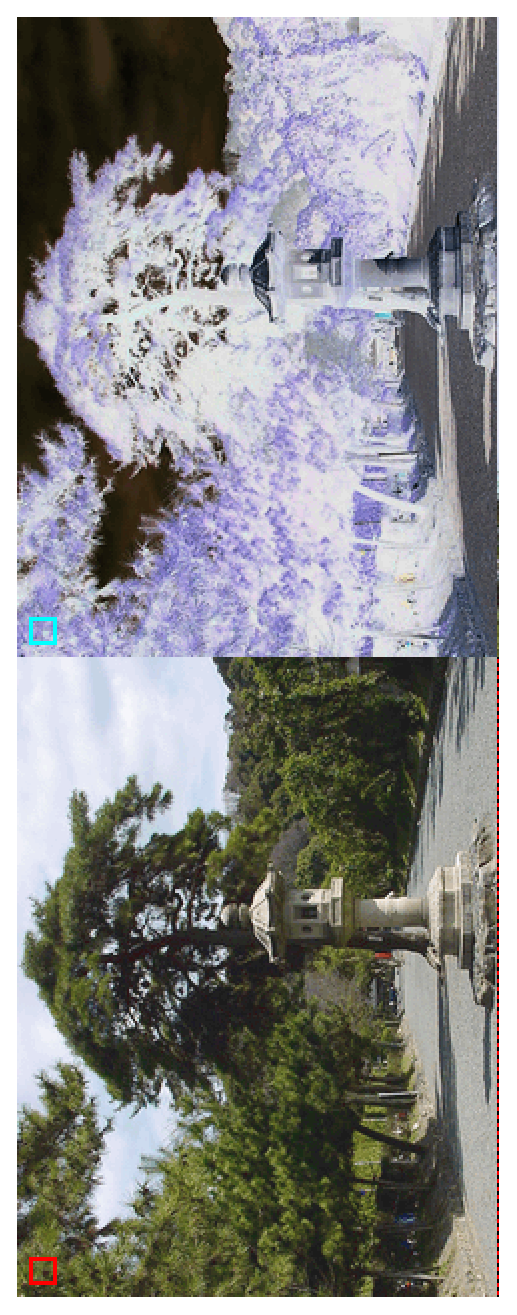
\includegraphics[angle=270,origin=b,width=0.75\textwidth]{tone_curve.eps}
\caption{Tone curve}
\end{figure}

Performs color conversion on an image based on the conversion table for each RGB color. By one burst operation, 6 rows of EMAX are configured (RMGRP = 6) to calculate for 10 locations (OMAP = 10). Mapdist = 0 because it is not a stencil calculation. Performance can be improved by PLOAD using unused stages.

\begin{screen}
\tiny
\begin{verbatim}
void tone_curve(Uint *r, Uint *d, Uchar *t) /* R, D, lut */
#if !defined(EMAX5) && !defined(EMAX6)
  for (top=PAD; top<HT-PAD; top++) { /* will be parallelized by multi-chip (M/#chip) */
    for (cofs=PAD; cofs<WD-PAD; cofs++) {
      Uint pix = *(r+top*WD+cofs);
      *(d+top*WD+cofs) = ((t)[pix>>24])<<24 | (t[256+((pix>>16)&255)])<<16 | (t[512+((pix>>8)&255)])<<8;
    }
  }
#endif
\end{verbatim}
\end{screen}

\begin{screen}
\tiny
\begin{verbatim}
  for (top=0; top<RRANGE; top+=RMGRP) { /* will be parallelized by multi-chip (M/#chip) */
    for (CHIP=0; CHIP<NCHIP; CHIP++) { /* will be parallelized by multi-chip (M/#chip) */
      for (rofs=0; rofs<RMGRP; rofs++) { /* will be parallelized by multi-chip (M/#chip) */
        int idx = (CHIP*RRANGE*OMAP+top+rofs)*WD;
        for (cofs=PAD; cofs<WD-PAD; cofs++) {
          for (oc=0; oc<OMAP; oc++) {
            Uint pix = *(r+idx+oc*RRANGE*WD+cofs);
            *(d+idx+oc*RRANGE*WD+cofs) = ((t)[pix>>24])<<24 | (t[256+((pix>>16)&255)])<<16 | (t[512+((pix>>8)&255)])<<8;
          }
        }
      }
    }
  }
\end{verbatim}
\end{screen}

\begin{screen}
\tiny
\begin{verbatim}
  Ull  LOOP1, LOOP0;
  Ull  INIT1, INIT0;
  Ull  AR[64][4];                     /* output of EX     in each unit */
  Ull  BR[64][4][4];                  /* output registers in each unit */
  Ull  r0, r1, r2, r3, r4, r5, r6, r7, r8, r9, r10, r11, r12, r13, r14, r15;
  Ull  r16, r17, r18, r19, r20, r21, r22, r23, r24, r25, r26, r27, r28, r29, r30, r31;
  Ull  cc0, cc1, cc2, cc3, ex0, ex1;
  for (top=0; top<RRANGE; top+=RMGRP) {
    Ull  rtop0[NCHIP], dtop0[NCHIP];
    Ull  rtop1[NCHIP], dtop1[NCHIP];
    Ull  rtop2[NCHIP], dtop2[NCHIP];
    Ull  rtop3[NCHIP], dtop3[NCHIP];
    Ull  rtop4[NCHIP], dtop4[NCHIP];
    Ull  rtop5[NCHIP], dtop5[NCHIP];
    Ull  rtop6[NCHIP], dtop6[NCHIP];
    Ull  rtop7[NCHIP], dtop7[NCHIP];
    Ull  rtop8[NCHIP], dtop8[NCHIP];
    Ull  rtop9[NCHIP], dtop9[NCHIP];
    for (CHIP=0; CHIP<NCHIP; CHIP++) { /* output channels are parallelized by multi-chip (OC/#chip) */
      rtop0[CHIP] = r+(CHIP*RRANGE*OMAP+RRANGE*0+top)*WD; dtop0[CHIP] = d+(CHIP*RRANGE*OMAP+RRANGE*0+top)*WD;
        :
      rtop9[CHIP] = r+(CHIP*RRANGE*OMAP+RRANGE*9+top)*WD; dtop9[CHIP] = d+(CHIP*RRANGE*OMAP+RRANGE*9+top)*WD;
    }
//EMAX5A begin tone_curve mapdist=0
    for (CHIP=0; CHIP<NCHIP; CHIP++) { /* output channels are parallelized by multi-chip (OC/#chip) */
 /*2*/for (INIT1=1,LOOP1=RMGRP,rofs=0-WD*4; LOOP1--; INIT1=0) {      /* stage#0 *//* mapped to FOR() on BR[63][1][0] */
   /*1*/for (INIT0=1,LOOP0=WD,cofs=0-4; LOOP0--; INIT0=0) {          /* stage#0 *//* mapped to FOR() on BR[63][0][0] */
          exe(OP_ADD,  &cofs, INIT0?cofs:cofs, EXP_H3210, 4, EXP_H3210, 0LL, EXP_H3210, OP_AND, 0x00000000ffffffffLL, OP_NOP, 0LL);  /* stage#0 */
          exe(OP_ADD,  &rofs, rofs, EXP_H3210, INIT0?WD*4:0, EXP_H3210, 0LL, EXP_H3210, OP_NOP, 0LL, OP_NOP, 0LL);                   /* stage#0 */
          exe(OP_ADD,  &pofs, rofs, EXP_H3210, cofs, EXP_H3210, 0LL, EXP_H3210, OP_AND, 0x00000000ffffffffLL, OP_NOP, 0LL);          /* stage#1 */
          /*map0*/
          mop(OP_LDWR,  1, &BR[2][1][1], (Ull)rtop0[CHIP], pofs,  MSK_D0, (Ull)rtop0[CHIP], WD*RMGRP, 0, 0, (Ull)NULL, WD*RMGRP);    /* stage#2 */
          mop(OP_LDBR,  1, &BR[3][1][1], (Ull)t1,    BR[2][1][1], MSK_B3, (Ull)t1, 256/4,  0,  0, (Ull)NULL, 256/4);                 /* stage#3 */
          mop(OP_LDBR,  1, &BR[3][2][1], (Ull)t2,    BR[2][1][1], MSK_B2, (Ull)t2, 256/4,  0,  0, (Ull)NULL, 256/4);                 /* stage#3 */
          mop(OP_LDBR,  1, &BR[3][3][1], (Ull)t3,    BR[2][1][1], MSK_B1, (Ull)t3, 256/4,  0,  0, (Ull)NULL, 256/4);                 /* stage#3 */
          exe(OP_MMRG, &r1, BR[3][1][1], EXP_H3210,  BR[3][2][1], EXP_H3210, BR[3][3][1], EXP_H3210, OP_NOP, 0LL, OP_NOP, 0LL);      /* stage#3 */
          mop(OP_STWR,  3, &r1,          (Ull)dtop0[CHIP], pofs,  MSK_D0, (Ull)dtop0[CHIP], WD*RMGRP, 0, 0, (Ull)NULL, WD*RMGRP);    /* stage#3 */
             :
          /*map5*/
          mop(OP_LDWR,  1, &BR[12][1][1],(Ull)rtop5[CHIP], pofs,  MSK_D0, (Ull)rtop5[CHIP], WD*RMGRP, 0, 0, (Ull)NULL, WD*RMGRP);    /* stage#12 */
          mop(OP_LDBR,  1, &BR[13][1][1],(Ull)t1,    BR[12][1][1],MSK_B3, (Ull)t1, 256/4,  0,  0, (Ull)NULL, 256/4);                 /* stage#13 */
          mop(OP_LDBR,  1, &BR[13][2][1],(Ull)t2,    BR[12][1][1],MSK_B2, (Ull)t2, 256/4,  0,  0, (Ull)NULL, 256/4);                 /* stage#13 */
          mop(OP_LDBR,  1, &BR[13][3][1],(Ull)t3,    BR[12][1][1],MSK_B1, (Ull)t3, 256/4,  0,  0, (Ull)NULL, 256/4);                 /* stage#13 */
          exe(OP_MMRG, &r1, BR[13][1][1],EXP_H3210,  BR[13][2][1],EXP_H3210, BR[13][3][1],EXP_H3210, OP_NOP, 0LL, OP_NOP, 0LL);      /* stage#13 */
          mop(OP_STWR,  3, &r1,          (Ull)dtop5[CHIP], pofs,  MSK_D0, (Ull)dtop5[CHIP], WD*RMGRP, 0, 0, (Ull)NULL, WD*RMGRP);    /* stage#13 */
          /*map6*/
          mop(OP_LDWR,  1, &BR[14][1][1],(Ull)rtop6[CHIP], pofs,  MSK_D0, (Ull)rtop6[CHIP], WD*RMGRP, 0, 0, (Ull)NULL, WD*RMGRP);    /* stage#14 */
          mop(OP_LDBR,  1, &BR[15][1][1],(Ull)t1,    BR[14][1][1],MSK_B3, (Ull)t1, 256/4,  0,  0, (Ull)NULL, 256/4);                 /* stage#15 */
          mop(OP_LDBR,  1, &BR[15][2][1],(Ull)t2,    BR[14][1][1],MSK_B2, (Ull)t2, 256/4,  0,  0, (Ull)NULL, 256/4);                 /* stage#15 */
          mop(OP_LDBR,  1, &BR[15][3][1],(Ull)t3,    BR[14][1][1],MSK_B1, (Ull)t3, 256/4,  0,  0, (Ull)NULL, 256/4);                 /* stage#15 */
          exe(OP_MMRG, &r1, BR[15][1][1],EXP_H3210,  BR[15][2][1],EXP_H3210, BR[15][3][1],EXP_H3210, OP_NOP, 0LL, OP_NOP, 0LL);      /* stage#15 */
          mop(OP_STWR,  3, &r1,          (Ull)dtop6[CHIP], pofs,  MSK_D0, (Ull)dtop6[CHIP], WD*RMGRP, 0, 0, (Ull)NULL, WD*RMGRP);    /* stage#15 */
          /*map7*/
          mop(OP_LDWR,  1, &BR[16][1][1],(Ull)rtop7[CHIP], pofs,  MSK_D0, (Ull)rtop7[CHIP], WD*RMGRP, 0, 0, (Ull)NULL, WD*RMGRP);    /* stage#16 */
          mop(OP_LDBR,  1, &BR[17][1][1],(Ull)t1,    BR[16][1][1],MSK_B3, (Ull)t1, 256/4,  0,  0, (Ull)NULL, 256/4);                 /* stage#17 */
          mop(OP_LDBR,  1, &BR[17][2][1],(Ull)t2,    BR[16][1][1],MSK_B2, (Ull)t2, 256/4,  0,  0, (Ull)NULL, 256/4);                 /* stage#17 */
          mop(OP_LDBR,  1, &BR[17][3][1],(Ull)t3,    BR[16][1][1],MSK_B1, (Ull)t3, 256/4,  0,  0, (Ull)NULL, 256/4);                 /* stage#17 */
          exe(OP_MMRG, &r1, BR[17][1][1],EXP_H3210,  BR[17][2][1],EXP_H3210, BR[17][3][1],EXP_H3210, OP_NOP, 0LL, OP_NOP, 0LL);      /* stage#17 */
          mop(OP_STWR,  3, &r1,          (Ull)dtop7[CHIP], pofs,  MSK_D0, (Ull)dtop7[CHIP], WD*RMGRP, 0, 0, (Ull)NULL, WD*RMGRP);    /* stage#17 */
          /*map8*/
          mop(OP_LDWR,  1, &BR[18][1][1],(Ull)rtop8[CHIP], pofs,  MSK_D0, (Ull)rtop8[CHIP], WD*RMGRP, 0, 0, (Ull)NULL, WD*RMGRP);    /* stage#18 */
          mop(OP_LDBR,  1, &BR[19][1][1],(Ull)t1,    BR[18][1][1],MSK_B3, (Ull)t1, 256/4,  0,  0, (Ull)NULL, 256/4);                 /* stage#19 */
          mop(OP_LDBR,  1, &BR[19][2][1],(Ull)t2,    BR[18][1][1],MSK_B2, (Ull)t2, 256/4,  0,  0, (Ull)NULL, 256/4);                 /* stage#19 */
          mop(OP_LDBR,  1, &BR[19][3][1],(Ull)t3,    BR[18][1][1],MSK_B1, (Ull)t3, 256/4,  0,  0, (Ull)NULL, 256/4);                 /* stage#19 */
          exe(OP_MMRG, &r1, BR[19][1][1],EXP_H3210,  BR[19][2][1],EXP_H3210, BR[19][3][1],EXP_H3210, OP_NOP, 0LL, OP_NOP, 0LL);      /* stage#19 */
          mop(OP_STWR,  3, &r1,          (Ull)dtop8[CHIP], pofs,  MSK_D0, (Ull)dtop8[CHIP], WD*RMGRP, 0, 0, (Ull)NULL, WD*RMGRP);    /* stage#19 */
          /*map9*/
          mop(OP_LDWR,  1, &BR[20][1][1],(Ull)rtop9[CHIP], pofs,  MSK_D0, (Ull)rtop9[CHIP], WD*RMGRP, 0, 0, (Ull)NULL, WD*RMGRP);    /* stage#20 */
          mop(OP_LDBR,  1, &BR[21][1][1],(Ull)t1,    BR[20][1][1],MSK_B3, (Ull)t1, 256/4,  0,  0, (Ull)NULL, 256/4);                 /* stage#21 */
          mop(OP_LDBR,  1, &BR[21][2][1],(Ull)t2,    BR[20][1][1],MSK_B2, (Ull)t2, 256/4,  0,  0, (Ull)NULL, 256/4);                 /* stage#21 */
          mop(OP_LDBR,  1, &BR[21][3][1],(Ull)t3,    BR[20][1][1],MSK_B1, (Ull)t3, 256/4,  0,  0, (Ull)NULL, 256/4);                 /* stage#21 */
          exe(OP_MMRG, &r1, BR[21][1][1],EXP_H3210,  BR[21][2][1],EXP_H3210, BR[21][3][1],EXP_H3210, OP_NOP, 0LL, OP_NOP, 0LL);      /* stage#21 */
          mop(OP_STWR,  3, &r1,          (Ull)dtop9[CHIP], pofs,  MSK_D0, (Ull)dtop9[CHIP], WD*RMGRP, 0, 0, (Ull)NULL, WD*RMGRP);    /* stage#21 */
    } } }
//EMAX5A end
  }
//EMAX5A drain_dirty_lmm
\end{verbatim}
\end{screen}

\begin{figure}[htbp]
\center
\epsfile{file=filter+rmm-tone_curve-emax6.eps,width=1.00\textwidth}
\caption{Tone curve}
\end{figure}

\clearpage

\subsection{Hokan1 with stencil}

\begin{figure}[htbp]
\center
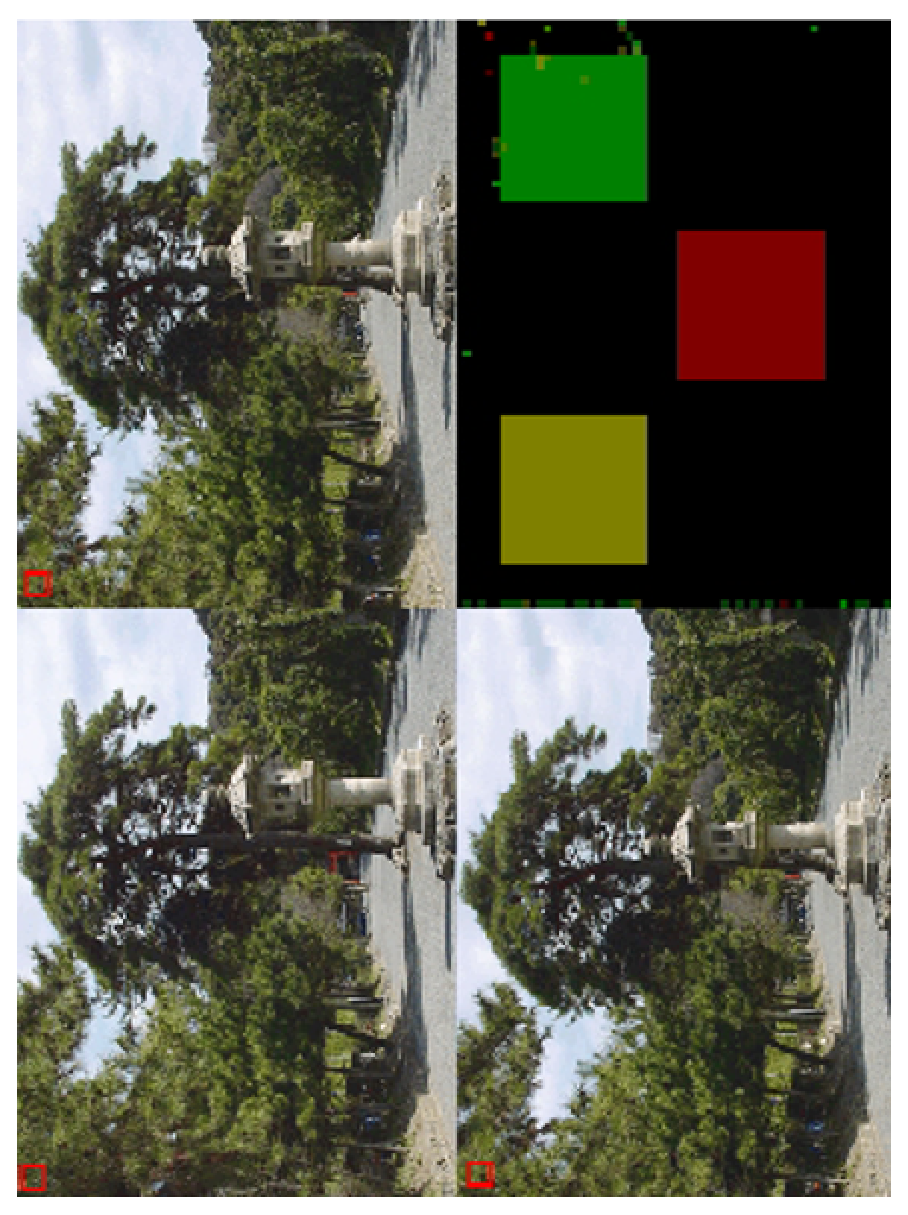
\includegraphics[angle=270,origin=b,width=0.50\textwidth]{hokan.eps}
\caption{Hokan}
\end{figure}

This is the first stage of frame interpolation. It finds the SAD values (4x4) for the 12x12 area and the 4x4 area. It performs SAD calculation for 8 rows by one burst operation (RMGRP = 8). This is a stencil calculation with mapdist = 7.

\begin{screen}
\tiny
\begin{verbatim}
void hokan1(Uint *c, Uint *p, struct SAD1 *s) /* W, R, SAD1 */
#if !defined(EMAX5) && !defined(EMAX6)
  for (top=PAD; top<HT-PAD; top++) { /* scan-lines */
    for (pofs=-4; pofs<4; pofs++) {
      Ushort *t = s->SAD1[top/4][pofs+4];
      for (cofs=0; cofs<WD; cofs++) {
        int j = cofs/4*4;
        int k = cofs%4*2;
        Uint *c2 = c+top*WD;
        Uint *p2 = p+(top+pofs)*WD;
        * t    += df(c2[j],p2[j+k-4]) + df(c2[j+1],p2[j+k-3]) + df(c2[j+2],p2[j+k-2]) + df(c2[j+3],p2[j+k-1]); /* p[-4],p[-3],p[-2],p[-1] -> p[-2],p[-1],p[0],p[1] */
        *(t+1) += df(c2[j],p2[j+k-3]) + df(c2[j+1],p2[j+k-2]) + df(c2[j+2],p2[j+k-1]) + df(c2[j+3],p2[j+k  ]); /* p[-3],p[-2],p[-1],p[ 0] -> p[-1],p[ 0],p[1],p[2] */
        t += 2;
  } } }
#endif
\end{verbatim}
\end{screen}

\begin{screen}
\tiny
\begin{verbatim}
  for (top=0; top<RRANGE; top+=RMGRP) {  /* will be parallelized by multi-chip (M/#chip) */
    for (rofs=0; rofs<RMGRP; rofs++) { /* will be parallelized by multi-chip (M/#chip) */
      for (CHIP=0; CHIP<NCHIP; CHIP++) {   /* will be parallelized by multi-chip (M/#chip) */
        int idx = CHIP*RRANGE+PAD+top+rofs;
        Uint *c0 = c+ idx   *WD;
        Uint *p0 = p+(idx-4)*WD;                                                                            /* j+k: 0,2,4,6; 4,6,8,10; 8,10,12,14; 12,14,16,18; */
        Uint *p1 = p+(idx-3)*WD;                                                                            /* j+k: 0,2,4,6; 4,6,8,10; 8,10,12,14; 12,14,16,18; */
        Uint *p2 = p+(idx-2)*WD;                                                                            /* j+k: 0,2,4,6; 4,6,8,10; 8,10,12,14; 12,14,16,18; */
        Uint *p3 = p+(idx-1)*WD;                                                                            /* j+k: 0,2,4,6; 4,6,8,10; 8,10,12,14; 12,14,16,18; */
        Uint *p4 = p+(idx+0)*WD;                                                                            /* j+k: 0,2,4,6; 4,6,8,10; 8,10,12,14; 12,14,16,18; */
        Uint *p5 = p+(idx+1)*WD;                                                                            /* j+k: 0,2,4,6; 4,6,8,10; 8,10,12,14; 12,14,16,18; */
        Uint *p6 = p+(idx+2)*WD;                                                                            /* j+k: 0,2,4,6; 4,6,8,10; 8,10,12,14; 12,14,16,18; */
        Uint *p7 = p+(idx+3)*WD;                                                                            /* j+k: 0,2,4,6; 4,6,8,10; 8,10,12,14; 12,14,16,18; */
        Ushort *t0 = s->SAD1[idx/4][0];
        Ushort *t1 = s->SAD1[idx/4][1];
        Ushort *t2 = s->SAD1[idx/4][2];
        Ushort *t3 = s->SAD1[idx/4][3];
        Ushort *t4 = s->SAD1[idx/4][4];
        Ushort *t5 = s->SAD1[idx/4][5];
        Ushort *t6 = s->SAD1[idx/4][6];
        Ushort *t7 = s->SAD1[idx/4][7];
        for (cofs=0; cofs<WD; cofs++) {
          int j = cofs/4*4;
          int k = cofs%4*2;
          * t0    += df(c0[j],p0[j+k-4]) + df(c0[j+1],p0[j+k-3]) + df(c0[j+2],p0[j+k-2]) + df(c0[j+3],p0[j+k-1]); /* p[-4],p[-3],p[-2],p[-1] -> p[-2],p[-1],p[0],p[1] */
          *(t0+1) += df(c0[j],p0[j+k-3]) + df(c0[j+1],p0[j+k-2]) + df(c0[j+2],p0[j+k-1]) + df(c0[j+3],p0[j+k  ]); /* p[-3],p[-2],p[-1],p[ 0] -> p[-1],p[ 0],p[1],p[2] */
          t0 += 2;
          * t1    += df(c0[j],p1[j+k-4]) + df(c0[j+1],p1[j+k-3]) + df(c0[j+2],p1[j+k-2]) + df(c0[j+3],p1[j+k-1]); /* p[-4],p[-3],p[-2],p[-1] -> p[-2],p[-1],p[0],p[1] */
          *(t1+1) += df(c0[j],p1[j+k-3]) + df(c0[j+1],p1[j+k-2]) + df(c0[j+2],p1[j+k-1]) + df(c0[j+3],p1[j+k  ]); /* p[-3],p[-2],p[-1],p[ 0] -> p[-1],p[ 0],p[1],p[2] */
          t1 += 2;
          * t2    += df(c0[j],p2[j+k-4]) + df(c0[j+1],p2[j+k-3]) + df(c0[j+2],p2[j+k-2]) + df(c0[j+3],p2[j+k-1]); /* p[-4],p[-3],p[-2],p[-1] -> p[-2],p[-1],p[0],p[1] */
          *(t2+1) += df(c0[j],p2[j+k-3]) + df(c0[j+1],p2[j+k-2]) + df(c0[j+2],p2[j+k-1]) + df(c0[j+3],p2[j+k  ]); /* p[-3],p[-2],p[-1],p[ 0] -> p[-1],p[ 0],p[1],p[2] */
          t2 += 2;
          * t3    += df(c0[j],p3[j+k-4]) + df(c0[j+1],p3[j+k-3]) + df(c0[j+2],p3[j+k-2]) + df(c0[j+3],p3[j+k-1]); /* p[-4],p[-3],p[-2],p[-1] -> p[-2],p[-1],p[0],p[1] */
          *(t3+1) += df(c0[j],p3[j+k-3]) + df(c0[j+1],p3[j+k-2]) + df(c0[j+2],p3[j+k-1]) + df(c0[j+3],p3[j+k  ]); /* p[-3],p[-2],p[-1],p[ 0] -> p[-1],p[ 0],p[1],p[2] */
          t3 += 2;
          * t4    += df(c0[j],p4[j+k-4]) + df(c0[j+1],p4[j+k-3]) + df(c0[j+2],p4[j+k-2]) + df(c0[j+3],p4[j+k-1]); /* p[-4],p[-3],p[-2],p[-1] -> p[-2],p[-1],p[0],p[1] */
          *(t4+1) += df(c0[j],p4[j+k-3]) + df(c0[j+1],p4[j+k-2]) + df(c0[j+2],p4[j+k-1]) + df(c0[j+3],p4[j+k  ]); /* p[-3],p[-2],p[-1],p[ 0] -> p[-1],p[ 0],p[1],p[2] */
          t4 += 2;
          * t5    += df(c0[j],p5[j+k-4]) + df(c0[j+1],p5[j+k-3]) + df(c0[j+2],p5[j+k-2]) + df(c0[j+3],p5[j+k-1]); /* p[-4],p[-3],p[-2],p[-1] -> p[-2],p[-1],p[0],p[1] */
          *(t5+1) += df(c0[j],p5[j+k-3]) + df(c0[j+1],p5[j+k-2]) + df(c0[j+2],p5[j+k-1]) + df(c0[j+3],p5[j+k  ]); /* p[-3],p[-2],p[-1],p[ 0] -> p[-1],p[ 0],p[1],p[2] */
          t5 += 2;
          * t6    += df(c0[j],p6[j+k-4]) + df(c0[j+1],p6[j+k-3]) + df(c0[j+2],p6[j+k-2]) + df(c0[j+3],p6[j+k-1]); /* p[-4],p[-3],p[-2],p[-1] -> p[-2],p[-1],p[0],p[1] */
          *(t6+1) += df(c0[j],p6[j+k-3]) + df(c0[j+1],p6[j+k-2]) + df(c0[j+2],p6[j+k-1]) + df(c0[j+3],p6[j+k  ]); /* p[-3],p[-2],p[-1],p[ 0] -> p[-1],p[ 0],p[1],p[2] */
          t6 += 2;
          * t7    += df(c0[j],p7[j+k-4]) + df(c0[j+1],p7[j+k-3]) + df(c0[j+2],p7[j+k-2]) + df(c0[j+3],p7[j+k-1]); /* p[-4],p[-3],p[-2],p[-1] -> p[-2],p[-1],p[0],p[1] */
          *(t7+1) += df(c0[j],p7[j+k-3]) + df(c0[j+1],p7[j+k-2]) + df(c0[j+2],p7[j+k-1]) + df(c0[j+3],p7[j+k  ]); /* p[-3],p[-2],p[-1],p[ 0] -> p[-1],p[ 0],p[1],p[2] */
          t7 += 2;
  } } } }
\end{verbatim}
\end{screen}

\begin{screen}
\tiny
\begin{verbatim}
  Ull  LOOP1, LOOP0;
  Ull  INIT1, INIT0;
  Ull  AR[64][4];                     /* output of EX     in each unit */
  Ull  BR[64][4][4];                  /* output registers in each unit */
  Ull  r0, r1, r2, r3, r4, r5, r6, r7, r8, r9, r10, r11, r12, r13, r14, r15;
  Ull  r16, r17, r18, r19, r20, r21, r22, r23, r24, r25, r26, r27, r28, r29, r30, r31;
  Ull  cc0, cc1, cc2, cc3, ex0, ex1;
  for (top=0; top<RRANGE; top+=RMGRP) {  /* will be parallelized by multi-chip (M/#chip) */
    for (rofs=0; rofs<RMGRP; rofs++) {      /* stage#0 *//* mapped to FOR() on BR[63][1][0] */
      Ull    jw, kw;
      Uint   *c0[NCHIP];
      Uint   *p0[NCHIP], *p1[NCHIP], *p2[NCHIP], *p3[NCHIP], *p4[NCHIP], *p5[NCHIP], *p6[NCHIP], *p7[NCHIP];
      Ushort *t0[NCHIP], *t1[NCHIP], *t2[NCHIP], *t3[NCHIP], *t4[NCHIP], *t5[NCHIP], *t6[NCHIP], *t7[NCHIP];
      for (CHIP=0; CHIP<NCHIP; CHIP++) {
        int idx = CHIP*RRANGE+PAD+top+rofs;
        c0[CHIP] = c+ idx   *WD;
        p0[CHIP] = p+(idx-4)*WD; /* j+k: 0,2,4,6; 4,6,8,10; 8,10,12,14; 12,14,16,18; */
        p1[CHIP] = p+(idx-3)*WD; /* j+k: 0,2,4,6; 4,6,8,10; 8,10,12,14; 12,14,16,18; */
        p2[CHIP] = p+(idx-2)*WD; /* j+k: 0,2,4,6; 4,6,8,10; 8,10,12,14; 12,14,16,18; */
        p3[CHIP] = p+(idx-1)*WD; /* j+k: 0,2,4,6; 4,6,8,10; 8,10,12,14; 12,14,16,18; */
        p4[CHIP] = p+(idx+0)*WD; /* j+k: 0,2,4,6; 4,6,8,10; 8,10,12,14; 12,14,16,18; */
        p5[CHIP] = p+(idx+1)*WD; /* j+k: 0,2,4,6; 4,6,8,10; 8,10,12,14; 12,14,16,18; */
        p6[CHIP] = p+(idx+2)*WD; /* j+k: 0,2,4,6; 4,6,8,10; 8,10,12,14; 12,14,16,18; */
        p7[CHIP] = p+(idx+3)*WD; /* j+k: 0,2,4,6; 4,6,8,10; 8,10,12,14; 12,14,16,18; */
        t0[CHIP] = s->SAD1[idx/4][0]; /* SAD1[HT/4][8][WD/4][8] ... [8][WD/4][8]=5120(2B) 0x1400 */
        t1[CHIP] = s->SAD1[idx/4][1];
        t2[CHIP] = s->SAD1[idx/4][2];
        t3[CHIP] = s->SAD1[idx/4][3];
        t4[CHIP] = s->SAD1[idx/4][4];
        t5[CHIP] = s->SAD1[idx/4][5];
        t6[CHIP] = s->SAD1[idx/4][6];
        t7[CHIP] = s->SAD1[idx/4][7];
      }
//EMAX5A begin hokan1 mapdist=7
 /*2*/for (CHIP=0; CHIP<NCHIP; CHIP++) { /* output channels are parallelized by multi-chip (OC/#chip) */
   /*1*/for (INIT0=1,LOOP0=WD,cofs=0-4; LOOP0--; INIT0=0) {       /* stage#0 *//* mapped to FOR() on BR[63][0][0] */
 /*@0,1*/ exe(OP_ADD,  &cofs, INIT0?cofs:cofs, EXP_H3210, 4, EXP_H3210, 0LL, EXP_H3210, OP_AND, 0x00000000ffffffffLL, OP_NOP, 0LL); /* stage#0 */
          /*int j = cofs/4 /4*4 *4;*/
          /*int k = cofs/4 %4*2 *4;*/
 /*@1,0*/ exe(OP_NOP,     &jw,          cofs,     EXP_H3210, 0LL, EXP_H3210, 0LL, EXP_H3210, OP_AND,~15LL, OP_SLL, 0LL);
 /*@1,1*/ exe(OP_NOP,     &kw,          cofs,     EXP_H3210, 0LL, EXP_H3210, 0LL, EXP_H3210, OP_AND, 12LL, OP_SLL, 1LL);
          /*k=-4*/
 /*@2,0*/ exe(OP_ADD,     &r12,         c0[CHIP], EXP_H3210, jw,  EXP_H3210, 0LL, EXP_H3210, OP_NOP,  0LL, OP_NOP, 0LL);
 /*@2,1*/ exe(OP_ADD3,    &r13,         p0[CHIP], EXP_H3210, jw,  EXP_H3210, kw,  EXP_H3210, OP_NOP,  0LL, OP_NOP, 0LL);
 /*@3,0*/ mop(OP_LDWR, 1, &r0,          r12,    0LL,  MSK_D0,  (Ull)c0[CHIP], WD, 0, 0, (Ull)NULL, WD);
 /*@3,1*/ mop(OP_LDWR, 1, &r1,          r12,    4LL,  MSK_D0,  (Ull)c0[CHIP], WD, 0, 0, (Ull)NULL, WD);
 /*@3,2*/ mop(OP_LDWR, 1, &r2,          r12,    8LL,  MSK_D0,  (Ull)c0[CHIP], WD, 0, 0, (Ull)NULL, WD);
 /*@3,3*/ mop(OP_LDWR, 1, &r3,          r12,   12LL,  MSK_D0,  (Ull)c0[CHIP], WD, 0, 0, (Ull)NULL, WD);
 /*@4,0*/ mop(OP_LDWR, 1, &BR[4][0][1], r13,  -16LL,  MSK_D0,  (Ull)p0[CHIP], WD, 0, 0, (Ull)NULL, WD);
 /*@4,1*/ mop(OP_LDWR, 1, &r25,         r13,  -12LL,  MSK_D0,  (Ull)p0[CHIP], WD, 0, 0, (Ull)NULL, WD);
 /*@4,2*/ mop(OP_LDWR, 1, &r26,         r13,   -8LL,  MSK_D0,  (Ull)p0[CHIP], WD, 0, 0, (Ull)NULL, WD);
 /*@4,3*/ mop(OP_LDWR, 1, &r27,         r13,   -4LL,  MSK_D0,  (Ull)p0[CHIP], WD, 0, 0, (Ull)NULL, WD);
 /*@4,3*/ mop(OP_LDWR, 1, &r28,         r13,    0LL,  MSK_D0,  (Ull)p0[CHIP], WD, 0, 0, (Ull)NULL, WD);
 /*@5,0*/ exe(OP_MSSAD,   &r11,         0LL,    EXP_H3210, r0,  EXP_H3210, r25, EXP_H3210, OP_NOP,  0LL, OP_NOP, 0LL);
 /*@5,1*/ exe(OP_MSSAD,   &r13,         0LL,    EXP_H3210, r1,  EXP_H3210, r26, EXP_H3210, OP_NOP,  0LL, OP_NOP, 0LL);
 /*@5,2*/ exe(OP_MSSAD,   &r15,         0LL,    EXP_H3210, r2,  EXP_H3210, r27, EXP_H3210, OP_NOP,  0LL, OP_NOP, 0LL);
 /*@5,3*/ exe(OP_MSSAD,   &r17,         0LL,    EXP_H3210, r3,  EXP_H3210, r28, EXP_H3210, OP_NOP,  0LL, OP_NOP, 0LL);
 /*@6,0*/ exe(OP_MSSAD,   &r10,         0LL,    EXP_H3210, r0,  EXP_H3210, BR[4][0][1], EXP_H3210, OP_NOP,  0LL, OP_NOP, 0LL);
 /*@6,1*/ exe(OP_MSSAD,   &r12,         0LL,    EXP_H3210, r1,  EXP_H3210, r25, EXP_H3210, OP_NOP,  0LL, OP_NOP, 0LL);
 /*@6,2*/ exe(OP_MSSAD,   &r14,         0LL,    EXP_H3210, r2,  EXP_H3210, r26, EXP_H3210, OP_NOP,  0LL, OP_NOP, 0LL);
 /*@6,3*/ exe(OP_MSSAD,   &r16,         0LL,    EXP_H3210, r3,  EXP_H3210, r27, EXP_H3210, OP_NOP,  0LL, OP_NOP, 0LL);
 /*@7,0*/ exe(OP_MAUH,    &r20,         r10,    EXP_H3210, r12, EXP_H3210, 0LL, EXP_H3210, OP_NOP,  0LL, OP_NOP, 0LL);
 /*@7,1*/ exe(OP_MAUH,    &r21,         r11,    EXP_H3210, r13, EXP_H3210, 0LL, EXP_H3210, OP_NOP,  0LL, OP_NOP, 0LL);
 /*@7,2*/ exe(OP_MAUH,    &r24,         r14,    EXP_H3210, r16, EXP_H3210, 0LL, EXP_H3210, OP_NOP,  0LL, OP_NOP, 0LL);
 /*@7,3*/ exe(OP_MAUH,    &r25,         r15,    EXP_H3210, r17, EXP_H3210, 0LL, EXP_H3210, OP_NOP,  0LL, OP_NOP, 0LL);
 /*@8,0*/ exe(OP_MAUH,    &r10,         r20,    EXP_H3210, r24, EXP_H3210, 0LL, EXP_H3210, OP_SUMHL,0LL, OP_NOP, 0LL);
 /*@8,1*/ exe(OP_MAUH,    &r11,         r21,    EXP_H3210, r25, EXP_H3210, 0LL, EXP_H3210, OP_SUMHH,0LL, OP_NOP, 0LL);
 /*@9,0*/ mop(OP_LDWR, 1, &BR[9][0][1], t0[CHIP],  cofs, MSK_D0, (Ull)t0[CHIP], WD, 0, 1, (Ull)NULL, WD);
 /*@9,0*/ exe(OP_MAUH3,   &AR[9][0],    BR[9][0][1],     EXP_H3210, r10, EXP_H3210, r11, EXP_H3210, OP_NOP, 0LL, OP_NOP, 0LL);
 /*@9,0*/ mop(OP_STWR, 3, &AR[9][0],    cofs,  t0[CHIP], MSK_D0, (Ull)t0[CHIP], WD, 0, 1, (Ull)NULL, WD);
     :
          /*k=+3*/
 /*@51,2*/exe(OP_ADD,     &r12,         c0[CHIP], EXP_H3210, jw,  EXP_H3210, 0LL, EXP_H3210, OP_NOP,  0LL, OP_NOP, 0LL);
 /*@51,3*/exe(OP_ADD3,    &r13,         p7[CHIP], EXP_H3210, jw,  EXP_H3210, kw,  EXP_H3210, OP_NOP,  0LL, OP_NOP, 0LL);
 /*@52,0*/mop(OP_LDWR, 1, &r0,          r12,    0LL,  MSK_D0,  (Ull)c0[CHIP], WD, 0, 0, (Ull)NULL, WD);
 /*@52,1*/mop(OP_LDWR, 1, &r1,          r12,    4LL,  MSK_D0,  (Ull)c0[CHIP], WD, 0, 0, (Ull)NULL, WD);
 /*@52,2*/mop(OP_LDWR, 1, &r2,          r12,    8LL,  MSK_D0,  (Ull)c0[CHIP], WD, 0, 0, (Ull)NULL, WD);
 /*@52,3*/mop(OP_LDWR, 1, &r3,          r12,   12LL,  MSK_D0,  (Ull)c0[CHIP], WD, 0, 0, (Ull)NULL, WD);
 /*@53,0*/mop(OP_LDWR, 1, &BR[53][0][1],r13,  -16LL,  MSK_D0,  (Ull)p7[CHIP], WD, 0, 0, (Ull)NULL, WD);
 /*@53,1*/mop(OP_LDWR, 1, &r25,         r13,  -12LL,  MSK_D0,  (Ull)p7[CHIP], WD, 0, 0, (Ull)NULL, WD);
 /*@53,2*/mop(OP_LDWR, 1, &r26,         r13,   -8LL,  MSK_D0,  (Ull)p7[CHIP], WD, 0, 0, (Ull)NULL, WD);
 /*@53,3*/mop(OP_LDWR, 1, &r27,         r13,   -4LL,  MSK_D0,  (Ull)p7[CHIP], WD, 0, 0, (Ull)NULL, WD);
 /*@53,3*/mop(OP_LDWR, 1, &r28,         r13,    0LL,  MSK_D0,  (Ull)p7[CHIP], WD, 0, 0, (Ull)NULL, WD);
 /*@54,0*/exe(OP_MSSAD,   &r11,         0LL,    EXP_H3210, r0,  EXP_H3210, r25, EXP_H3210, OP_NOP,  0LL, OP_NOP, 0LL);
 /*@54,1*/exe(OP_MSSAD,   &r13,         0LL,    EXP_H3210, r1,  EXP_H3210, r26, EXP_H3210, OP_NOP,  0LL, OP_NOP, 0LL);
 /*@54,2*/exe(OP_MSSAD,   &r15,         0LL,    EXP_H3210, r2,  EXP_H3210, r27, EXP_H3210, OP_NOP,  0LL, OP_NOP, 0LL);
 /*@54,3*/exe(OP_MSSAD,   &r17,         0LL,    EXP_H3210, r3,  EXP_H3210, r28, EXP_H3210, OP_NOP,  0LL, OP_NOP, 0LL);
 /*@55,0*/exe(OP_MSSAD,   &r10,         0LL,    EXP_H3210, r0,  EXP_H3210, BR[53][0][1], EXP_H3210, OP_NOP,  0LL, OP_NOP, 0LL);
 /*@55,1*/exe(OP_MSSAD,   &r12,         0LL,    EXP_H3210, r1,  EXP_H3210, r25, EXP_H3210, OP_NOP,  0LL, OP_NOP, 0LL);
 /*@55,2*/exe(OP_MSSAD,   &r14,         0LL,    EXP_H3210, r2,  EXP_H3210, r26, EXP_H3210, OP_NOP,  0LL, OP_NOP, 0LL);
 /*@55,3*/exe(OP_MSSAD,   &r16,         0LL,    EXP_H3210, r3,  EXP_H3210, r27, EXP_H3210, OP_NOP,  0LL, OP_NOP, 0LL);
 /*@56,0*/exe(OP_MAUH,    &r20,         r10,    EXP_H3210, r12, EXP_H3210, 0LL, EXP_H3210, OP_NOP,  0LL, OP_NOP, 0LL);
 /*@56,1*/exe(OP_MAUH,    &r21,         r11,    EXP_H3210, r13, EXP_H3210, 0LL, EXP_H3210, OP_NOP,  0LL, OP_NOP, 0LL);
 /*@56,2*/exe(OP_MAUH,    &r24,         r14,    EXP_H3210, r16, EXP_H3210, 0LL, EXP_H3210, OP_NOP,  0LL, OP_NOP, 0LL);
 /*@56,3*/exe(OP_MAUH,    &r25,         r15,    EXP_H3210, r17, EXP_H3210, 0LL, EXP_H3210, OP_NOP,  0LL, OP_NOP, 0LL);
 /*@57,0*/exe(OP_MAUH,    &r10,         r20,    EXP_H3210, r24, EXP_H3210, 0LL, EXP_H3210, OP_SUMHL,0LL, OP_NOP, 0LL);
 /*@57,1*/exe(OP_MAUH,    &r11,         r21,    EXP_H3210, r25, EXP_H3210, 0LL, EXP_H3210, OP_SUMHH,0LL, OP_NOP, 0LL);
 /*@58,0*/mop(OP_LDWR, 1, &BR[58][0][1],t7[CHIP],  cofs, MSK_D0, (Ull)t7[CHIP], WD, 0, 1, (Ull)NULL, WD);
 /*@58,0*/exe(OP_MAUH3,   &AR[58][0],   BR[58][0][1],    EXP_H3210, r10, EXP_H3210, r11, EXP_H3210, OP_NOP, 0LL, OP_NOP, 0LL);
 /*@58,0*/mop(OP_STWR, 3, &AR[58][0],   cofs,  t7[CHIP], MSK_D0, (Ull)t7[CHIP], WD, 0, 1, (Ull)NULL, WD);
        }
      }
//EMAX5A end
    }
  }
//EMAX5A drain_dirty_lmm
\end{verbatim}
\end{screen}

\begin{figure}[htbp]
\center
\epsfile{file=filter+rmm-hokan1-emax6.eps,width=1.00\textwidth}
\caption{Hokan1}
\end{figure}

\clearpage

\subsection{Hokan2 with stencil}

This is the second stage of frame interpolation. It finds the smallest SAD value from 4x4 SAD values and find the corresponding xy relative coordinates. The coordinates of 12 rows are calculated by one burst operation (RMGRP = 12). This is not stencil calculation, therefore Mapdist = 0.

\begin{screen}
\tiny
\begin{verbatim}
void hokan2(struct SAD1 *s, Uint *minxy) /* [WD/4][8] */
#if !defined(EMAX5) && !defined(EMAX6)
  for (top=PAD; top<HT-PAD; top+=4) { /* scan-lines */
    Uint *xy = minxy+top*WD;
    for (pofs=-4; pofs<4; pofs++) {
      Ushort *t  = s->SAD1[top/4][pofs+4];
      int    idx = ((pofs/2)&0xff)<<16;
      for (cofs=0; cofs<WD; cofs++) { /* j%4==0�λ��Τ�minxy[j]��ͭ���͡�¾�ϥ��� */
        int l1 = ((-2)<<24)|idx|*(t  ); if ((xy[cofs]&HM) > *(t  )) xy[cofs] = l1;
        int l2 = ((-1)<<24)|idx|*(t+1); if ((xy[cofs]&HM) > *(t+1)) xy[cofs] = l2;
        int l3 = ((-1)<<24)|idx|*(t+2); if ((xy[cofs]&HM) > *(t+2)) xy[cofs] = l3;
        int l4 = (( 0)<<24)|idx|*(t+3); if ((xy[cofs]&HM) > *(t+3)) xy[cofs] = l4;
        int l5 = (( 0)<<24)|idx|*(t+4); if ((xy[cofs]&HM) > *(t+4)) xy[cofs] = l5;
        int l6 = (( 0)<<24)|idx|*(t+5); if ((xy[cofs]&HM) > *(t+5)) xy[cofs] = l6;
        int l7 = (( 1)<<24)|idx|*(t+6); if ((xy[cofs]&HM) > *(t+6)) xy[cofs] = l7;
        int l8 = (( 1)<<24)|idx|*(t+7); if ((xy[cofs]&HM) > *(t+7)) xy[cofs] = l8;
        t += 2;
      }
    }
  }
#endif
\end{verbatim}
\end{screen}

\begin{screen}
\tiny
\begin{verbatim}
  Uint ix0 = ((-4/2)&0xff)<<16; /* -2,-1,-1,0,0,0,1,1 */
  Uint ix1 = ((-3/2)&0xff)<<16; /* -2,-1,-1,0,0,0,1,1 */
  Uint ix2 = ((-2/2)&0xff)<<16; /* -2,-1,-1,0,0,0,1,1 */
  Uint ix3 = ((-1/2)&0xff)<<16; /* -2,-1,-1,0,0,0,1,1 */
  Uint ix4 = (( 0/2)&0xff)<<16; /* -2,-1,-1,0,0,0,1,1 */
  Uint ix5 = ((+1/2)&0xff)<<16; /* -2,-1,-1,0,0,0,1,1 */
  Uint ix6 = ((+2/2)&0xff)<<16; /* -2,-1,-1,0,0,0,1,1 */
  Uint ix7 = ((+3/2)&0xff)<<16; /* -2,-1,-1,0,0,0,1,1 */
  for (top=0; top<RRANGE; top+=RMGRP) {  /* will be parallelized by multi-chip (M/#chip) */
    for (rofs=0; rofs<RMGRP; rofs+=4) { /* will be parallelized by multi-chip (M/#chip) */
      for (CHIP=0; CHIP<NCHIP; CHIP++) {   /* will be parallelized by multi-chip (M/#chip) */
        Ushort *t0 = s->SAD1[(CHIP*RRANGE+top+rofs)/4][0];
        Ushort *t1 = s->SAD1[(CHIP*RRANGE+top+rofs)/4][1];
        Ushort *t2 = s->SAD1[(CHIP*RRANGE+top+rofs)/4][2];
        Ushort *t3 = s->SAD1[(CHIP*RRANGE+top+rofs)/4][3];
        Ushort *t4 = s->SAD1[(CHIP*RRANGE+top+rofs)/4][4];
        Ushort *t5 = s->SAD1[(CHIP*RRANGE+top+rofs)/4][5];
        Ushort *t6 = s->SAD1[(CHIP*RRANGE+top+rofs)/4][6];
        Ushort *t7 = s->SAD1[(CHIP*RRANGE+top+rofs)/4][7];
        Uint   *xy = minxy+(CHIP*RRANGE+top+rofs)*WD;
        for (cofs=0; cofs<WD; cofs++) { /* j%4==0�λ��Τ�minxy[j]��ͭ���͡�¾�ϥ��� */
          int l1, l2, l3, l4, l5, l6, l7, l8;
          l1=((-2)<<24)|ix0|*(t0  ); if((xy[cofs]&HM)>*(t0  ))xy[cofs]=l1;
          l2=((-1)<<24)|ix0|*(t0+1); if((xy[cofs]&HM)>*(t0+1))xy[cofs]=l2;
          l3=((-1)<<24)|ix0|*(t0+2); if((xy[cofs]&HM)>*(t0+2))xy[cofs]=l3;
          l4=           ix0|*(t0+3); if((xy[cofs]&HM)>*(t0+3))xy[cofs]=l4;
          l5=           ix0|*(t0+4); if((xy[cofs]&HM)>*(t0+4))xy[cofs]=l5;
          l6=           ix0|*(t0+5); if((xy[cofs]&HM)>*(t0+5))xy[cofs]=l6;
          l7=(( 1)<<24)|ix0|*(t0+6); if((xy[cofs]&HM)>*(t0+6))xy[cofs]=l7;
          l8=(( 1)<<24)|ix0|*(t0+7); if((xy[cofs]&HM)>*(t0+7))xy[cofs]=l8;
          t0 += 2;
          l1=((-2)<<24)|ix1|*(t1  ); if((xy[cofs]&HM)>*(t1  ))xy[cofs]=l1;
          l2=((-1)<<24)|ix1|*(t1+1); if((xy[cofs]&HM)>*(t1+1))xy[cofs]=l2;
          l3=((-1)<<24)|ix1|*(t1+2); if((xy[cofs]&HM)>*(t1+2))xy[cofs]=l3;
          l4=           ix1|*(t1+3); if((xy[cofs]&HM)>*(t1+3))xy[cofs]=l4;
          l5=           ix1|*(t1+4); if((xy[cofs]&HM)>*(t1+4))xy[cofs]=l5;
          l6=           ix1|*(t1+5); if((xy[cofs]&HM)>*(t1+5))xy[cofs]=l6;
          l7=(( 1)<<24)|ix1|*(t1+6); if((xy[cofs]&HM)>*(t1+6))xy[cofs]=l7;
          l8=(( 1)<<24)|ix1|*(t1+7); if((xy[cofs]&HM)>*(t1+7))xy[cofs]=l8;
             :
          t5 += 2;
          l1=((-2)<<24)|ix6|*(t6  ); if((xy[cofs]&HM)>*(t6  ))xy[cofs]=l1;
          l2=((-1)<<24)|ix6|*(t6+1); if((xy[cofs]&HM)>*(t6+1))xy[cofs]=l2;
          l3=((-1)<<24)|ix6|*(t6+2); if((xy[cofs]&HM)>*(t6+2))xy[cofs]=l3;
          l4=           ix6|*(t6+3); if((xy[cofs]&HM)>*(t6+3))xy[cofs]=l4;
          l5=           ix6|*(t6+4); if((xy[cofs]&HM)>*(t6+4))xy[cofs]=l5;
          l6=           ix6|*(t6+5); if((xy[cofs]&HM)>*(t6+5))xy[cofs]=l6;
          l7=(( 1)<<24)|ix6|*(t6+6); if((xy[cofs]&HM)>*(t6+6))xy[cofs]=l7;
          l8=(( 1)<<24)|ix6|*(t6+7); if((xy[cofs]&HM)>*(t6+7))xy[cofs]=l8;
          t6 += 2;
          l1=((-2)<<24)|ix7|*(t7  ); if((xy[cofs]&HM)>*(t7  ))xy[cofs]=l1;
          l2=((-1)<<24)|ix7|*(t7+1); if((xy[cofs]&HM)>*(t7+1))xy[cofs]=l2;
          l3=((-1)<<24)|ix7|*(t7+2); if((xy[cofs]&HM)>*(t7+2))xy[cofs]=l3;
          l4=           ix7|*(t7+3); if((xy[cofs]&HM)>*(t7+3))xy[cofs]=l4;
          l5=           ix7|*(t7+4); if((xy[cofs]&HM)>*(t7+4))xy[cofs]=l5;
          l6=           ix7|*(t7+5); if((xy[cofs]&HM)>*(t7+5))xy[cofs]=l6;
          l7=(( 1)<<24)|ix7|*(t7+6); if((xy[cofs]&HM)>*(t7+6))xy[cofs]=l7;
          l8=(( 1)<<24)|ix7|*(t7+7); if((xy[cofs]&HM)>*(t7+7))xy[cofs]=l8;
          t7 += 2;
        }
      }
    }
  }
\end{verbatim}
\end{screen}

\begin{screen}
\tiny
\begin{verbatim}
  Ull  LOOP1, LOOP0;
  Ull  INIT1, INIT0;
  Ull  AR[64][4];                     /* output of EX     in each unit */
  Ull  BR[64][4][4];                  /* output registers in each unit */
  Ull  r0, r1, r2, r3, r4, r5, r6, r7, r8, r9, r10, r11, r12, r13, r14, r15;
  Ull  r16, r17, r18, r19, r20, r21, r22, r23, r24, r25, r26, r27, r28, r29, r30, r31;
  Ull  cc0, cc1, cc2, cc3, ex0, ex1;
  Uint ix0 = ((-4/2)&0xff)<<16; /* -2,-1,-1,0,0,0,1,1 */
  Uint ix1 = ((-3/2)&0xff)<<16; /* -2,-1,-1,0,0,0,1,1 */
  Uint ix2 = ((-2/2)&0xff)<<16; /* -2,-1,-1,0,0,0,1,1 */
  Uint ix3 = ((-1/2)&0xff)<<16; /* -2,-1,-1,0,0,0,1,1 */
  Uint ix4 = (( 0/2)&0xff)<<16; /* -2,-1,-1,0,0,0,1,1 */
  Uint ix5 = ((+1/2)&0xff)<<16; /* -2,-1,-1,0,0,0,1,1 */
  Uint ix6 = ((+2/2)&0xff)<<16; /* -2,-1,-1,0,0,0,1,1 */
  Uint ix7 = ((+3/2)&0xff)<<16; /* -2,-1,-1,0,0,0,1,1 */
  for (top=0; top<RRANGE; top+=RMGRP) {  /* will be parallelized by multi-chip (M/#chip) */
    for (rofs=0; rofs<RMGRP; rofs+=4) { /* will be parallelized by multi-chip (M/#chip) */
      Uint *xy[NCHIP];
      Uint *t00[NCHIP],*t10[NCHIP],*t20[NCHIP],*t30[NCHIP],*t40[NCHIP],*t50[NCHIP],*t60[NCHIP],*t70[NCHIP];
      Uint *t01[NCHIP],*t11[NCHIP],*t21[NCHIP],*t31[NCHIP],*t41[NCHIP],*t51[NCHIP],*t61[NCHIP],*t71[NCHIP];
      Uint *t02[NCHIP],*t12[NCHIP],*t22[NCHIP],*t32[NCHIP],*t42[NCHIP],*t52[NCHIP],*t62[NCHIP],*t72[NCHIP];
      Uint *t03[NCHIP],*t13[NCHIP],*t23[NCHIP],*t33[NCHIP],*t43[NCHIP],*t53[NCHIP],*t63[NCHIP],*t73[NCHIP];
      for (CHIP=0; CHIP<NCHIP; CHIP++) {   /* will be parallelized by multi-chip (M/#chip) */
        int idx = CHIP*RRANGE+PAD+top+rofs;
        t00[CHIP] = s->SAD1[idx/4][0]; t01[CHIP] = t00[CHIP]+1; t02[CHIP] = t00[CHIP]+2; t03[CHIP] = t00[CHIP]+3;
        t10[CHIP] = s->SAD1[idx/4][1]; t11[CHIP] = t10[CHIP]+1; t12[CHIP] = t10[CHIP]+2; t13[CHIP] = t10[CHIP]+3;
        t20[CHIP] = s->SAD1[idx/4][2]; t21[CHIP] = t20[CHIP]+1; t22[CHIP] = t20[CHIP]+2; t23[CHIP] = t20[CHIP]+3;
        t30[CHIP] = s->SAD1[idx/4][3]; t31[CHIP] = t30[CHIP]+1; t32[CHIP] = t30[CHIP]+2; t33[CHIP] = t30[CHIP]+3;
        t40[CHIP] = s->SAD1[idx/4][4]; t41[CHIP] = t40[CHIP]+1; t42[CHIP] = t40[CHIP]+2; t43[CHIP] = t40[CHIP]+3;
        t50[CHIP] = s->SAD1[idx/4][5]; t51[CHIP] = t50[CHIP]+1; t52[CHIP] = t50[CHIP]+2; t53[CHIP] = t50[CHIP]+3;
        t60[CHIP] = s->SAD1[idx/4][6]; t61[CHIP] = t60[CHIP]+1; t62[CHIP] = t60[CHIP]+2; t63[CHIP] = t60[CHIP]+3;
        t70[CHIP] = s->SAD1[idx/4][7]; t71[CHIP] = t70[CHIP]+1; t72[CHIP] = t70[CHIP]+2; t73[CHIP] = t70[CHIP]+3;
        xy[CHIP] = minxy+idx*WD;
      }
//EMAX5A begin hokan2 mapdist=0
 /*2*/for (CHIP=0; CHIP<NCHIP; CHIP++) { /* output channels are parallelized by multi-chip (OC/#chip) */
   /*1*/for (INIT0=1,LOOP0=WD,cofs=0-4; LOOP0--; INIT0=0) {       /* stage#0 *//* mapped to FOR() on BR[63][0][0] */
 /*@0,1*/ exe(OP_ADD,     &cofs,  INIT0?cofs:cofs, EXP_H3210, 4,           EXP_H3210, 0LL,  EXP_H3210, OP_AND, 0x00000000ffffffffLL, OP_NOP, 0LL);
          /*k=-4*/
 /*@1,0*/ mop(OP_LDWR, 1, &r10,         t00[CHIP], cofs,      MSK_D0,      t00[CHIP], WD, 0, 0, (Ull)NULL, WD);
 /*@1,0*/ exe(OP_NOP,     &r28,        (-2LL<<24), EXP_H3210, 0,           EXP_H3210, 0LL,  EXP_H3210, OP_OR,   ix0, OP_NOP, 0LL);
 /*@1,0*/ mop(OP_LDWR, 1, &r12,         t01[CHIP], cofs,      MSK_D0,      t00[CHIP], WD, 0, 0, (Ull)NULL, WD);
 /*@1,1*/ exe(OP_NOP,     &r29,        (-1LL<<24), EXP_H3210, 0,           EXP_H3210, 0LL,  EXP_H3210, OP_OR,   ix0, OP_NOP, 0LL);
 /*@1,1*/ mop(OP_LDWR, 1, &r14,         t02[CHIP], cofs,      MSK_D0,      t00[CHIP], WD, 0, 0, (Ull)NULL, WD);
 /*@1,2*/ exe(OP_NOP,     &r31,        ( 1LL<<24), EXP_H3210, 0,           EXP_H3210, 0LL,  EXP_H3210, OP_OR,   ix0, OP_NOP, 0LL);
 /*@1,2*/ mop(OP_LDWR, 1, &r16,         t03[CHIP], cofs,      MSK_D0,      t00[CHIP], WD, 0, 0, (Ull)NULL, WD);
 /*@2,0*/ exe(OP_MINL3,   &r10,         r29,       EXP_H3210, r28,         EXP_H3210, r10,  EXP_H3210, OP_NOP,  0LL, OP_NOP, 0LL);
 /*@2,1*/ exe(OP_MINL3,   &r12,         ix0,       EXP_H3210, r29,         EXP_H3210, r12,  EXP_H3210, OP_NOP,  0LL, OP_NOP, 0LL);
 /*@2,2*/ exe(OP_MINL3,   &r14,         ix0,       EXP_H3210, ix0,         EXP_H3210, r14,  EXP_H3210, OP_NOP,  0LL, OP_NOP, 0LL);
 /*@2,3*/ exe(OP_MINL3,   &r16,         r31,       EXP_H3210, r31,         EXP_H3210, r16,  EXP_H3210, OP_NOP,  0LL, OP_NOP, 0LL);
 /*@3,0*/ exe(OP_MINL,    &r20,         r10,       EXP_H3210, r12,         EXP_H3210, 0LL,  EXP_H3210, OP_NOP,  0LL, OP_NOP, 0LL);
 /*@3,1*/ exe(OP_MINL,    &r24,         r14,       EXP_H3210, r16,         EXP_H3210, 0LL,  EXP_H3210, OP_NOP,  0LL, OP_NOP, 0LL);
 /*@4,0*/ exe(OP_MINL,    &r0,          r20,       EXP_H3210, r24,         EXP_H3210, 0LL,  EXP_H3210, OP_NOP,  0LL, OP_NOP, 0LL);
          /*k=-3*/
 /*@4,0*/ mop(OP_LDWR, 1, &r10,         t10[CHIP], cofs,      MSK_D0,      t10[CHIP], WD, 0, 0, (Ull)NULL, WD);
 /*@4,1*/ exe(OP_NOP,     &r28,        (-2LL<<24), EXP_H3210, 0,           EXP_H3210, 0LL,  EXP_H3210, OP_OR,   ix1, OP_NOP, 0LL);
 /*@4,1*/ mop(OP_LDWR, 1, &r12,         t11[CHIP], cofs,      MSK_D0,      t10[CHIP], WD, 0, 0, (Ull)NULL, WD);
 /*@4,2*/ exe(OP_NOP,     &r29,        (-1LL<<24), EXP_H3210, 0,           EXP_H3210, 0LL,  EXP_H3210, OP_OR,   ix1, OP_NOP, 0LL);
 /*@4,2*/ mop(OP_LDWR, 1, &r14,         t12[CHIP], cofs,      MSK_D0,      t10[CHIP], WD, 0, 0, (Ull)NULL, WD);
 /*@4,3*/ exe(OP_NOP,     &r31,        ( 1LL<<24), EXP_H3210, 0,           EXP_H3210, 0LL,  EXP_H3210, OP_OR,   ix1, OP_NOP, 0LL);
 /*@4,3*/ mop(OP_LDWR, 1, &r16,         t13[CHIP], cofs,      MSK_D0,      t10[CHIP], WD, 0, 0, (Ull)NULL, WD);
 /*@5,0*/ exe(OP_MINL3,   &r10,         r29,       EXP_H3210, r28,         EXP_H3210, r10,  EXP_H3210, OP_NOP,  0LL, OP_NOP, 0LL);
 /*@5,1*/ exe(OP_MINL3,   &r12,         ix1,       EXP_H3210, r29,         EXP_H3210, r12,  EXP_H3210, OP_NOP,  0LL, OP_NOP, 0LL);
 /*@5,2*/ exe(OP_MINL3,   &r14,         ix1,       EXP_H3210, ix1,         EXP_H3210, r14,  EXP_H3210, OP_NOP,  0LL, OP_NOP, 0LL);
 /*@5,3*/ exe(OP_MINL3,   &r16,         r31,       EXP_H3210, r31,         EXP_H3210, r16,  EXP_H3210, OP_NOP,  0LL, OP_NOP, 0LL);
 /*@6,0*/ exe(OP_MINL,    &r20,         r10,       EXP_H3210, r12,         EXP_H3210, 0LL,  EXP_H3210, OP_NOP,  0LL, OP_NOP, 0LL);
 /*@6,1*/ exe(OP_MINL,    &r24,         r14,       EXP_H3210, r16,         EXP_H3210, 0LL,  EXP_H3210, OP_NOP,  0LL, OP_NOP, 0LL);
 /*@7,0*/ exe(OP_MINL,    &r1,          r20,       EXP_H3210, r24,         EXP_H3210, 0LL,  EXP_H3210, OP_NOP,  0LL, OP_NOP, 0LL);
 /*@8,0*/ exe(OP_MINL,    &r0,          r1,        EXP_H3210, r0,          EXP_H3210, 0LL,  EXP_H3210, OP_NOP,  0LL, OP_NOP, 0LL);
      :
          /*k=2*/
 /*@24,0*/mop(OP_LDWR, 1, &r10,         t60[CHIP], cofs,      MSK_D0,      t60[CHIP], WD, 0, 0, (Ull)NULL, WD);
 /*@24,1*/exe(OP_NOP,     &r28,        (-2LL<<24), EXP_H3210, 0,           EXP_H3210, 0LL,  EXP_H3210, OP_OR,   ix6, OP_NOP, 0LL);
 /*@24,1*/mop(OP_LDWR, 1, &r12,         t61[CHIP], cofs,      MSK_D0,      t60[CHIP], WD, 0, 0, (Ull)NULL, WD);
 /*@24,2*/exe(OP_NOP,     &r29,        (-1LL<<24), EXP_H3210, 0,           EXP_H3210, 0LL,  EXP_H3210, OP_OR,   ix6, OP_NOP, 0LL);
 /*@24,2*/mop(OP_LDWR, 1, &r14,         t62[CHIP], cofs,      MSK_D0,      t60[CHIP], WD, 0, 0, (Ull)NULL, WD);
 /*@24,3*/exe(OP_NOP,     &r31,        ( 1LL<<24), EXP_H3210, 0,           EXP_H3210, 0LL,  EXP_H3210, OP_OR,   ix6, OP_NOP, 0LL);
 /*@24,3*/mop(OP_LDWR, 1, &r16,         t63[CHIP], cofs,      MSK_D0,      t60[CHIP], WD, 0, 0, (Ull)NULL, WD);
 /*@25,0*/exe(OP_MINL3,   &r10,         r29,       EXP_H3210, r28,         EXP_H3210, r10,  EXP_H3210, OP_NOP,  0LL, OP_NOP, 0LL);
 /*@25,1*/exe(OP_MINL3,   &r12,         ix6,       EXP_H3210, r29,         EXP_H3210, r12,  EXP_H3210, OP_NOP,  0LL, OP_NOP, 0LL);
 /*@25,2*/exe(OP_MINL3,   &r14,         ix6,       EXP_H3210, ix6,         EXP_H3210, r14,  EXP_H3210, OP_NOP,  0LL, OP_NOP, 0LL);
 /*@25,3*/exe(OP_MINL3,   &r16,         r31,       EXP_H3210, r31,         EXP_H3210, r16,  EXP_H3210, OP_NOP,  0LL, OP_NOP, 0LL);
 /*@26,0*/exe(OP_MINL,    &r20,         r10,       EXP_H3210, r12,         EXP_H3210, 0LL,  EXP_H3210, OP_NOP,  0LL, OP_NOP, 0LL);
 /*@26,1*/exe(OP_MINL,    &r24,         r14,       EXP_H3210, r16,         EXP_H3210, 0LL,  EXP_H3210, OP_NOP,  0LL, OP_NOP, 0LL);
 /*@27,0*/exe(OP_MINL,    &r1,          r20,       EXP_H3210, r24,         EXP_H3210, 0LL,  EXP_H3210, OP_NOP,  0LL, OP_NOP, 0LL);
 /*@28,0*/exe(OP_MINL,    &r0,          r1,        EXP_H3210, r0,          EXP_H3210, 0LL,  EXP_H3210, OP_NOP,  0LL, OP_NOP, 0LL);
          /*k=3*/
 /*@28,0*/mop(OP_LDWR, 1, &r10,         t70[CHIP], cofs,      MSK_D0,      t70[CHIP], WD, 0, 0, (Ull)NULL, WD);
 /*@28,1*/exe(OP_NOP,     &r28,        (-2LL<<24), EXP_H3210, 0,           EXP_H3210, 0LL,  EXP_H3210, OP_OR,   ix7, OP_NOP, 0LL);
 /*@28,1*/mop(OP_LDWR, 1, &r12,         t71[CHIP], cofs,      MSK_D0,      t70[CHIP], WD, 0, 0, (Ull)NULL, WD);
 /*@28,2*/exe(OP_NOP,     &r29,        (-1LL<<24), EXP_H3210, 0,           EXP_H3210, 0LL,  EXP_H3210, OP_OR,   ix7, OP_NOP, 0LL);
 /*@28,2*/mop(OP_LDWR, 1, &r14,         t72[CHIP], cofs,      MSK_D0,      t70[CHIP], WD, 0, 0, (Ull)NULL, WD);
 /*@28,3*/exe(OP_NOP,     &r31,        ( 1LL<<24), EXP_H3210, 0,           EXP_H3210, 0LL,  EXP_H3210, OP_OR,   ix7, OP_NOP, 0LL);
 /*@28,3*/mop(OP_LDWR, 1, &r16,         t73[CHIP], cofs,      MSK_D0,      t70[CHIP], WD, 0, 0, (Ull)NULL, WD);
 /*@29,0*/exe(OP_MINL3,   &r10,         r29,       EXP_H3210, r28,         EXP_H3210, r10,  EXP_H3210, OP_NOP,  0LL, OP_NOP, 0LL);
 /*@29,1*/exe(OP_MINL3,   &r12,         ix7,       EXP_H3210, r29,         EXP_H3210, r12,  EXP_H3210, OP_NOP,  0LL, OP_NOP, 0LL);
 /*@29,2*/exe(OP_MINL3,   &r14,         ix7,       EXP_H3210, ix7,         EXP_H3210, r14,  EXP_H3210, OP_NOP,  0LL, OP_NOP, 0LL);
 /*@29,3*/exe(OP_MINL3,   &r16,         r31,       EXP_H3210, r31,         EXP_H3210, r16,  EXP_H3210, OP_NOP,  0LL, OP_NOP, 0LL);
 /*@30,0*/exe(OP_MINL,    &r20,         r10,       EXP_H3210, r12,         EXP_H3210, 0LL,  EXP_H3210, OP_NOP,  0LL, OP_NOP, 0LL);
 /*@30,1*/exe(OP_MINL,    &r24,         r14,       EXP_H3210, r16,         EXP_H3210, 0LL,  EXP_H3210, OP_NOP,  0LL, OP_NOP, 0LL);
 /*@31,0*/exe(OP_MINL,    &r1,          r20,       EXP_H3210, r24,         EXP_H3210, 0LL,  EXP_H3210, OP_NOP,  0LL, OP_NOP, 0LL);
 /*@32,0*/exe(OP_MINL,    &r0,          r1,        EXP_H3210, r0,          EXP_H3210, 0LL,  EXP_H3210, OP_NOP,  0LL, OP_NOP, 0LL);
 /*@33,0*/mop(OP_LDWR, 1, &BR[33][0][1],xy[CHIP],  cofs,      MSK_D0,      xy[CHIP],  WD, 0, 1, (Ull)NULL, WD);
 /*@33,0*/exe(OP_MINL,    &AR[33][0],   r0,        EXP_H3210, BR[33][0][1],EXP_H3210, 0LL,  EXP_H3210, OP_NOP,  0LL, OP_NOP, 0LL);
 /*@33,0*/mop(OP_STWR, 3, &AR[33][0],   cofs,      xy[CHIP],  MSK_D0,      xy[CHIP],  WD, 0, 1, (Ull)NULL, WD);
        }
      }
//EMAX5A end
    }
  }
//EMAX5A drain_dirty_lmm
\end{verbatim}
\end{screen}

\begin{figure}[htbp]
\center
\epsfile{file=filter+rmm-hokan2-emax6.eps,width=1.00\textwidth}
\caption{Hokan2}
\end{figure}

\clearpage

\subsection{Hokan3 with stencil}

This is the third stage of frame interpolation. It pastes the reference image based on the xy relative coordinates in the direction of high similarity. The pasting process for 12 rows is performed by one burst operation (RMGRP = 12). Mapdist = 0 because it is not a stencil calculation.

\begin{screen}
\tiny
\begin{verbatim}
void hokan3(Uint *minxy, Uint *r, Uint *d)
#if !defined(EMAX5) && !defined(EMAX6)
  for (top=PAD; top<HT-PAD; top++) { /* scan-lines */
    Uint *xy = minxy+(top/4*4)*WD;
    Uint *dp = d+top*WD;
    for (pofs=-2; pofs<2; pofs++) {
      Uint *rp = r+(top+pofs)*WD;
      for (cofs=0; cofs<WD; cofs++) {
        int x = (int) xy[cofs/4*4]>>24;
        int y = (int)(xy[cofs/4*4]<<8)>>24;
        if (y == pofs) dp[cofs] = rp[cofs+x];
      }
    }
  }
#endif
\end{verbatim}
\end{screen}

\begin{screen}
\tiny
\begin{verbatim}
  for (top=0; top<RRANGE; top+=RMGRP) { /* will be parallelized by multi-chip (M/#chip) */
    for (rofs=0; rofs<RMGRP; rofs++) { /* will be parallelized by multi-chip (M/#chip) */
      for (CHIP=0; CHIP<NCHIP; CHIP++) { /* will be parallelized by multi-chip (M/#chip) */
        int idx = CHIP*RRANGE+top+rofs;
        Uint *xy = minxy+(idx/4*4)*WD;
        Uint *dp = d+idx*WD;
        Uint *rp0 = r+(idx-2)*WD;
        Uint *rp1 = r+(idx-1)*WD;
        Uint *rp2 = r+(idx+0)*WD;
        Uint *rp3 = r+(idx+1)*WD;
        for (cofs=0; cofs<WD; cofs++) {
          int x = (int) xy[cofs/4*4]>>24;
          int y = (int)(xy[cofs/4*4]<<8)>>24;
          dp[cofs] = (y == -2)?rp0[cofs+x]:
                     (y == -1)?rp1[cofs+x]:
                     (y ==  0)?rp2[cofs+x]:
                     (y ==  1)?rp3[cofs+x]:0;
        }
      }
    }
  }
\end{verbatim}
\end{screen}

\begin{screen}
\tiny
\begin{verbatim}
  Ull  LOOP1, LOOP0;
  Ull  INIT1, INIT0;
  Ull  AR[64][4];                     /* output of EX     in each unit */
  Ull  BR[64][4][4];                  /* output registers in each unit */
  Ull  r0, r1, r2, r3, r4, r5, r6, r7, r8, r9, r10, r11, r12, r13, r14, r15;
  Ull  r16, r17, r18, r19, r20, r21, r22, r23, r24, r25, r26, r27, r28, r29, r30, r31;
  Ull  cc0, cc1, cc2, cc3, ex0, ex1;
  for (top=0; top<RRANGE; top+=RMGRP) { /* will be parallelized by multi-chip (M/#chip) */
    for (rofs=0; rofs<RMGRP; rofs++) { /* will be parallelized by multi-chip (M/#chip) */
      Ull  jw;
      Uint *xy[NCHIP], *dp[NCHIP], *rp0[NCHIP], *rp1[NCHIP], *rp2[NCHIP], *rp3[NCHIP];
      for (CHIP=0; CHIP<NCHIP; CHIP++) { /* will be parallelized by multi-chip (M/#chip) */
        int idx   = CHIP*RRANGE+top+rofs;
        xy[CHIP]  = minxy+(idx/4*4)*WD;
        dp[CHIP]  = d+idx*WD;
        rp0[CHIP] = r+(idx-2)*WD;
        rp1[CHIP] = r+(idx-1)*WD;
        rp2[CHIP] = r+(idx+0)*WD;
        rp3[CHIP] = r+(idx+1)*WD;
      }
//EMAX5A begin hokan3 mapdist=0
 /*2*/for (CHIP=0; CHIP<NCHIP; CHIP++) { /* output channels are parallelized by multi-chip (OC/#chip) */
   /*1*/for (INIT0=1,LOOP0=WD,cofs=0-4; LOOP0--; INIT0=0) {       /* stage#0 *//* mapped to FOR() on BR[63][0][0] */
 /*@0,1*/ exe(OP_ADD,     &cofs, INIT0?cofs:cofs, EXP_H3210, 4, EXP_H3210, 0LL, EXP_H3210, OP_AND, 0x00000000ffffffffLL, OP_NOP, 0LL);
 /*@1,0*/ exe(OP_NOP,     &jw,   cofs, EXP_H3210, 0LL,  EXP_H3210, 0LL, EXP_H3210, OP_AND, ~15LL,         OP_SLL,   0LL);

 /*@2,0*/ mop(OP_LDWR, 1, &r10,  xy[CHIP],    jw, MSK_D0,   xy[CHIP],   WD,    0, 0, (Ull)NULL,       WD);
 /*@3,0*/ exe(OP_NOP,     &r2,   r10,  EXP_H3210, 0LL,  EXP_H3210, 0LL, EXP_H3210, OP_AND,  0xff000000LL, OP_SRAA, 22LL); /*x*/
 /*@3,1*/ exe(OP_NOP,     &r3,   r10,  EXP_H3210, 0LL,  EXP_H3210, 0LL, EXP_H3210, OP_AND,  0x00ff0000LL, OP_SRAB, 16LL); /*y*/
 /*@4,0*/ exe(OP_ADD,     &r4,   r2,   EXP_H3210, cofs, EXP_H3210, 0LL, EXP_H3210, OP_NOP,  0LL,          OP_NOP,   0LL);

 /*@5,0*/ mop(OP_LDWR, 1, &r10,  rp0[CHIP],  r4,  MSK_D0,    rp0[CHIP], WD,    0, 0, (Ull)NULL,       WD);            /*rp0[cofs+x]*/
 /*@5,0*/ exe(OP_CMP_EQ,  &r5,   r3,  EXP_H3210, -2,   EXP_H3210, 0LL, EXP_H3210, OP_NOP,  0LL,          OP_NOP,   0LL);  /*y==-2?*/
 /*@6,0*/ exe(OP_CMOV,    &r0,   r5,  EXP_H3210, r10,  EXP_H3210, 0LL, EXP_H3210, OP_NOP,  0LL,          OP_NOP,   0LL);

 /*@6,0*/ mop(OP_LDWR, 1, &r10,  rp1[CHIP],  r4,  MSK_D0,    rp1[CHIP], WD,    0, 0, (Ull)NULL,       WD);            /*rp1[cofs+x]*/
 /*@6,1*/ exe(OP_CMP_EQ,  &r5,   r3,  EXP_H3210, -1,   EXP_H3210, 0LL, EXP_H3210, OP_NOP,  0LL,          OP_NOP,   0LL);  /*y==-1?*/
 /*@7,0*/ exe(OP_CMOV,    &r0,   r5,  EXP_H3210, r10,  EXP_H3210,  r0, EXP_H3210, OP_NOP,  0LL,          OP_NOP,   0LL);

 /*@7,0*/ mop(OP_LDWR, 1, &r10,  rp2[CHIP],  r4,  MSK_D0,    rp2[CHIP], WD,    0, 0, (Ull)NULL,       WD);            /*rp2[cofs+x]*/
 /*@7,1*/ exe(OP_CMP_EQ,  &r5,   r3,  EXP_H3210,  0,   EXP_H3210, 0LL, EXP_H3210, OP_NOP,  0LL,          OP_NOP,   0LL);  /*y== 0?*/
 /*@8,0*/ exe(OP_CMOV,    &r0,   r5,  EXP_H3210, r10,  EXP_H3210,  r0, EXP_H3210, OP_NOP,  0LL,          OP_NOP,   0LL);

 /*@8,0*/ mop(OP_LDWR, 1, &r10,  rp3[CHIP],  r4,  MSK_D0,    rp3[CHIP], WD,    0, 0, (Ull)NULL,       WD);            /*rp3[cofs+x]*/
 /*@8,1*/ exe(OP_CMP_EQ,  &r5,   r3,  EXP_H3210,  1,   EXP_H3210, 0LL, EXP_H3210, OP_NOP,  0LL,          OP_NOP,   0LL);  /*y== 1?*/
 /*@9,0*/ exe(OP_CMOV,    &r0,   r5,  EXP_H3210, r10,  EXP_H3210,  r0, EXP_H3210, OP_NOP,  0LL,          OP_NOP,   0LL);
 /*@9,0*/ mop(OP_STWR, 3, &r0,   dp[CHIP],  cofs, MSK_D0,     dp[CHIP], WD,    0, 1, (Ull)NULL,       WD);
        }
      }
//EMAX5A end
    }
  }
//EMAX5A drain_dirty_lmm
\end{verbatim}
\end{screen}

\begin{figure}[htbp]
\center
\epsfile{file=filter+rmm-hokan3-emax6.eps,width=1.00\textwidth}
\caption{Hokan3}
\end{figure}

\clearpage

\subsection{Expand4k with stencil}

\begin{figure}[htbp]
\center
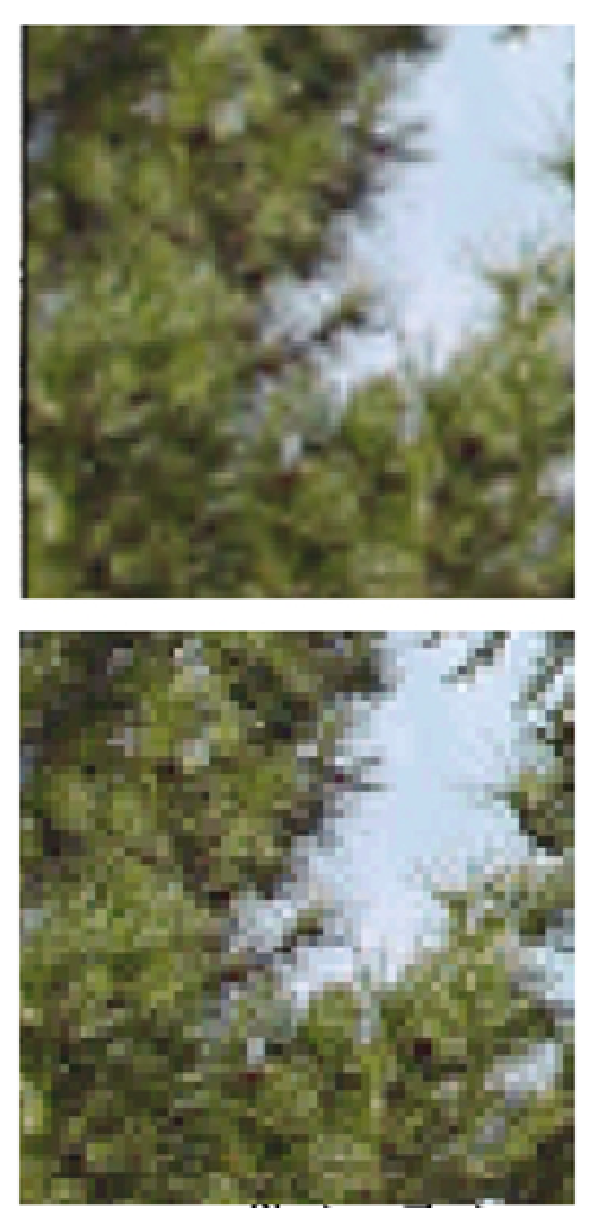
\includegraphics[angle=270,origin=b,width=0.75\textwidth]{expand4k.eps}
\caption{Expand4k}
\end{figure}

This is a Super-resolution processing. It generates a high-resolution image by interpolating a low-resolution image. It performs interpolation processing for 12 rows by one burst operation (RMGRP = 12). Because the moving distance of the input image is not constant, it is not a stencil calculation, therefore mapdist = 0.


\begin{screen}
\tiny
\begin{verbatim}
void expand4k(Uint *p, struct X *r)
#if !defined(EMAX5) && !defined(EMAX6)
  for (top=0; top<RRANGE; top+=RMGRP) { /* scan-lines */
    for (rofs=0; rofs<RMGRP; rofs++) { /* will be parallelized by multi-chip (M/#chip) */
      for (CHIP=0; CHIP<NCHIP; CHIP++) { /* will be parallelized by multi-chip (M/#chip) */
        int idx = CHIP*RRANGE+top+rofs;
        int k = idx*HT/768;
        int kfraq = (((idx*HT)<<4)/768)&15; /* 4bit */
        int kad = 16-ad(kfraq,8);
        int sk1 = ss(kfraq,8);
        int sk2 = ss(8,kfraq);
        Uint *pp = p+k*WD;
        Uint *rp = r->X[idx];
        for (cofs=0; cofs<1024; cofs++) { /* ������4095�ޤ� */
          int p1 = cofs*WD/1024;
          int lfraq = (((cofs*WD)<<4)/1024)&15; /* 4bit */
          int lad = 16-ad(lfraq,8);
          int sl1 = ss(lfraq,8);
          int sl2 = ss(8,lfraq);
          int r1 = kad*lad; /* 4bit*4bit */
          int r3 = kad*sl1; /* 4bit*4bit */
          int r2 = kad*sl2; /* 4bit*4bit */
          int r5 = sk1*lad; /* 4bit*4bit */
          int r9 = sk1*sl1; /* 4bit*4bit */
          int r8 = sk1*sl2; /* 4bit*4bit */
          int r4 = sk2*lad; /* 4bit*4bit */
          int r7 = sk2*sl1; /* 4bit*4bit */
          int r6 = sk2*sl2; /* 4bit*4bit */
          *rp = (unsigned int)((pp[p1]>>24&0xff)*r1
              +  (pp[p1   -1]>>24&0xff)*r2 + (pp[p1   +1]>>24&0xff)*r3 + (pp[p1-WD  ]>>24&0xff)*r4 + (pp[p1+WD  ]>>24&0xff)*r5
              +  (pp[p1-WD-1]>>24&0xff)*r6 + (pp[p1-WD+1]>>24&0xff)*r7 + (pp[p1+WD-1]>>24&0xff)*r8 + (pp[p1+WD+1]>>24&0xff)*r9)/256<<24
              | (unsigned int)((pp[p1]>>16&0xff)*r1
              +  (pp[p1   -1]>>16&0xff)*r2 + (pp[p1   +1]>>16&0xff)*r3 + (pp[p1-WD  ]>>16&0xff)*r4 + (pp[p1+WD  ]>>16&0xff)*r5
              +  (pp[p1-WD-1]>>16&0xff)*r6 + (pp[p1-WD+1]>>16&0xff)*r7 + (pp[p1+WD-1]>>16&0xff)*r8 + (pp[p1+WD+1]>>16&0xff)*r9)/256<<16
              | (unsigned int)((pp[p1]>> 8&0xff)*r1
              +  (pp[p1   -1]>> 8&0xff)*r2 + (pp[p1   +1]>> 8&0xff)*r3 + (pp[p1-WD  ]>> 8&0xff)*r4 + (pp[p1+WD  ]>> 8&0xff)*r5
              +  (pp[p1-WD-1]>> 8&0xff)*r6 + (pp[p1-WD+1]>> 8&0xff)*r7 + (pp[p1+WD-1]>> 8&0xff)*r8 + (pp[p1+WD+1]>> 8&0xff)*r9)/256<<8;
          rp++;
        }
      }
    }
  }
#endif
\end{verbatim}
\end{screen}

\begin{screen}
\tiny
\begin{verbatim}
  for (top=0; top<RRANGE; top+=RMGRP) { /* scan-lines */
    for (rofs=0; rofs<RMGRP; rofs++) { /* will be parallelized by multi-chip (M/#chip) */
      for (CHIP=0; CHIP<NCHIP; CHIP++) { /* will be parallelized by multi-chip (M/#chip) */
        int idx = CHIP*RRANGE+top+rofs;
        int k = idx*HT/768;
        int kfraq = (((idx*HT)<<4)/768)&15; /* 4bit */
        int kad = 16-ad(kfraq,8);
        int sk1 = ss(kfraq,8);
        int sk2 = ss(8,kfraq);
        Uint *pp = p+k*WD;
        Uint *rp = r->X[idx];
        for (cofs=0; cofs<1024; cofs++) { /* ������4095�ޤ� */
          int p1 = cofs*WD/1024;
          int lfraq = (((cofs*WD)<<4)/1024)&15; /* 4bit */
          int lad = 16-ad(lfraq,8);
          int sl1 = ss(lfraq,8);
          int sl2 = ss(8,lfraq);
          int r1 = kad*lad; /* 4bit*4bit */
          int r3 = kad*sl1; /* 4bit*4bit */
          int r2 = kad*sl2; /* 4bit*4bit */
          int r5 = sk1*lad; /* 4bit*4bit */
          int r9 = sk1*sl1; /* 4bit*4bit */
          int r8 = sk1*sl2; /* 4bit*4bit */
          int r4 = sk2*lad; /* 4bit*4bit */
          int r7 = sk2*sl1; /* 4bit*4bit */
          int r6 = sk2*sl2; /* 4bit*4bit */
          Uint ph, pl, x;
          ph = madd(mmul(b2h(pp[p1     ], 1), r1), mmul(b2h(pp[p1-1], 1), r2));
          ph = madd(mmul(b2h(pp[p1   +1], 1), r3), ph);
          ph = madd(mmul(b2h(pp[p1-WD  ], 1), r4), ph);
          ph = madd(mmul(b2h(pp[p1+WD  ], 1), r5), ph);
          ph = madd(mmul(b2h(pp[p1-WD-1], 1), r6), ph);
          ph = madd(mmul(b2h(pp[p1-WD+1], 1), r7), ph);
          ph = madd(mmul(b2h(pp[p1+WD-1], 1), r8), ph);
          ph = madd(mmul(b2h(pp[p1+WD+1], 1), r9), ph);
          pl = madd(mmul(b2h(pp[p1     ], 0), r1), mmul(b2h(pp[p1-1], 0), r2));
          pl = madd(mmul(b2h(pp[p1   +1], 0), r3), pl);
          pl = madd(mmul(b2h(pp[p1-WD  ], 0), r4), pl);
          pl = madd(mmul(b2h(pp[p1+WD  ], 0), r5), pl);
          pl = madd(mmul(b2h(pp[p1-WD-1], 0), r6), pl);
          pl = madd(mmul(b2h(pp[p1-WD+1], 0), r7), pl);
          pl = madd(mmul(b2h(pp[p1+WD-1], 0), r8), pl);
          pl = madd(mmul(b2h(pp[p1+WD+1], 0), r9), pl);
          *rp = h2b(msrl(ph, 8), 1) | h2b(msrl(pl, 8), 0);
          rp++;
        }
      }
    }
  }
\end{verbatim}
\end{screen}

\begin{screen}
\tiny
\begin{verbatim}
  Ull  LOOP1, LOOP0;
  Ull  INIT1, INIT0;
  Ull  AR[64][4];                     /* output of EX     in each unit */
  Ull  BR[64][4][4];                  /* output registers in each unit */
  Ull  r0, r1, r2, r3, r4, r5, r6, r7, r8, r9, r10, r11, r12, r13, r14, r15;
  Ull  r16, r17, r18, r19, r20, r21, r22, r23, r24, r25, r26, r27, r28, r29, r30, r31;
  Ull  cc0, cc1, cc2, cc3, ex0, ex1;
  for (top=0; top<RRANGE; top+=RMGRP) { /* will be parallelized by multi-chip (M/#chip) */
    for (rofs=0; rofs<RMGRP; rofs++) { /* will be parallelized by multi-chip (M/#chip) */
      Sll  kad[NCHIP], sk1[NCHIP], sk2[NCHIP];
      Uint *pp[NCHIP], *p0[NCHIP], *p1[NCHIP], *p2[NCHIP], *rp[NCHIP];
      for (CHIP=0; CHIP<NCHIP; CHIP++) { /* will be parallelized by multi-chip (M/#chip) */
        int  idx   = CHIP*RRANGE+top+rofs;
        int  k     = idx*HT/768;
        int  kfraq = (((idx*HT)<<4)/768)&15; /* 4bit */
        kad[CHIP]  = 16-ad(kfraq,8);
        sk1[CHIP]  = ss(kfraq,8);
        sk2[CHIP]  = ss(8,kfraq);
        pp[CHIP]   = p+k*WD;
        p0[CHIP]   = pp[CHIP]-WD;
        p1[CHIP]   = pp[CHIP];
        p2[CHIP]   = pp[CHIP]+WD;
        rp[CHIP]   = r->X[idx];
      }
//EMAX5A begin expand4k mapdist=0
 /*2*/for (CHIP=0; CHIP<NCHIP; CHIP++) { /* output channels are parallelized by multi-chip (OC/#chip) */
   /*1*/for (INIT0=1,LOOP0=1024,cofs=0-WD; LOOP0--; INIT0=0) {       /* stage#0 *//* mapped to FOR() on BR[63][0][0] */
 /*@0,1*/ exe(OP_ADD,       &cofs, cofs,      EXP_H3210, WD,    EXP_H3210, 0LL, EXP_H3210, OP_AND, 0x00000000ffffffffLL, OP_NOP, 0LL);
 /*@1,0*/ exe(OP_NOP,       &r0,   cofs,      EXP_H3210, 0LL,   EXP_H3210, 0LL, EXP_H3210, OP_AND, ~1023LL,  OP_SRL,  8LL);
 /*@1,1*/ exe(OP_NOP,       &r4,   cofs,      EXP_H3210, 0LL,   EXP_H3210, 0LL, EXP_H3210, OP_AND,  0x3c0LL, OP_SRL,  6LL);
 /*@2,0*/ exe(OP_ADD,       &r0,   pp[CHIP],  EXP_H3210, r0,    EXP_H3210, 0LL, EXP_H3210, OP_NOP,  0LL,     OP_NOP,  0LL);
 /*@2,1*/ exe(OP_MSUH,      &r1,   r4,        EXP_H3210, 8LL,   EXP_H3210, 0LL, EXP_H3210, OP_NOP,  0LL,     OP_NOP,  0LL);
 /*@2,2*/ exe(OP_MSUH,      &r2,   8LL,       EXP_H3210, r4,    EXP_H3210, 0LL, EXP_H3210, OP_NOP,  0LL,     OP_NOP,  0LL);
 /*@2,3*/ exe(OP_MSSAD,     &r3,   0LL,       EXP_H3210, r4,    EXP_H3210, 8LL, EXP_H3210, OP_NOP,  0LL,     OP_NOP,  0LL);
 /*@3,3*/ exe(OP_MSUH,      &r3,   16LL,      EXP_H3210, r3,    EXP_H3210, 0LL, EXP_H3210, OP_NOP,  0LL,     OP_NOP,  0LL);

 /*@4,1*/ exe(OP_MLUH,      &r21,  sk2[CHIP], EXP_H3210, r1,    EXP_H3210, 0LL, EXP_H3210, OP_NOP,  0LL,     OP_NOP,  0LL);
 /*@4,1*/ mop(OP_LDWR, 1,   &r10,  r0, -1276, MSK_D0,    (Ull)p0[CHIP],    WD,    0, 0, (Ull)NULL,       WD);
 /*@4,2*/ exe(OP_MLUH,      &r22,  sk2[CHIP], EXP_H3210, r2,    EXP_H3210, 0LL, EXP_H3210, OP_NOP,  0LL,     OP_NOP,  0LL);
 /*@4,2*/ mop(OP_LDWR, 1,   &r11,  r0, -1284, MSK_D0,    (Ull)p0[CHIP],    WD,    0, 0, (Ull)NULL,       WD);
 /*@4,3*/ exe(OP_MLUH,      &r23,  sk2[CHIP], EXP_H3210, r3,    EXP_H3210, 0LL, EXP_H3210, OP_NOP,  0LL,     OP_NOP,  0LL);
 /*@4,3*/ mop(OP_LDWR, 1,   &r12,  r0, -1280, MSK_D0,    (Ull)p0[CHIP],    WD,    0, 0, (Ull)NULL,       WD);

 /*@5,1*/ exe(OP_MLUH,      &r13,  r10,       EXP_B5410, r21,   EXP_H3210, 0LL, EXP_H3210, OP_NOP,  0LL,     OP_NOP,  0LL);
 /*@5,2*/ exe(OP_MLUH,      &r14,  r11,       EXP_B5410, r22,   EXP_H3210, 0LL, EXP_H3210, OP_NOP,  0LL,     OP_NOP,  0LL);
 /*@5,3*/ exe(OP_MLUH,      &r15,  r12,       EXP_B5410, r23,   EXP_H3210, 0LL, EXP_H3210, OP_NOP,  0LL,     OP_NOP,  0LL);

 /*@6,0*/ exe(OP_MAUH3,     &r16,  r13,       EXP_H3210, r14,   EXP_H3210, r15, EXP_H3210, OP_NOP,  0LL,     OP_NOP,  0LL);
 /*@6,1*/ exe(OP_MLUH,      &r13,  r10,       EXP_B7632, r21,   EXP_H3210, 0LL, EXP_H3210, OP_NOP,  0LL,     OP_NOP,  0LL);
 /*@6,2*/ exe(OP_MLUH,      &r14,  r11,       EXP_B7632, r22,   EXP_H3210, 0LL, EXP_H3210, OP_NOP,  0LL,     OP_NOP,  0LL);
 /*@6,3*/ exe(OP_MLUH,      &r15,  r12,       EXP_B7632, r23,   EXP_H3210, 0LL, EXP_H3210, OP_NOP,  0LL,     OP_NOP,  0LL);

 /*@7,0*/ exe(OP_MAUH3,     &r17,  r13,       EXP_H3210, r14,   EXP_H3210, r15, EXP_H3210, OP_NOP,  0LL,     OP_NOP,  0LL);
 /*@7,1*/ exe(OP_MLUH,      &r21,  kad[CHIP], EXP_H3210, r1,    EXP_H3210, 0LL, EXP_H3210, OP_NOP,  0LL,     OP_NOP,  0LL);
 /*@7,1*/ mop(OP_LDWR, 1,   &r10,  r0,     4, MSK_D0,    (Ull)p1[CHIP],    WD,    0, 0, (Ull)NULL,       WD);
 /*@7,2*/ exe(OP_MLUH,      &r22,  kad[CHIP], EXP_H3210, r2,    EXP_H3210, 0LL, EXP_H3210, OP_NOP,  0LL,     OP_NOP,  0LL);
 /*@7,2*/ mop(OP_LDWR, 1,   &r11,  r0,    -4, MSK_D0,    (Ull)p1[CHIP],    WD,    0, 0, (Ull)NULL,       WD);
 /*@7,3*/ exe(OP_MLUH,      &r23,  kad[CHIP], EXP_H3210, r3,    EXP_H3210, 0LL, EXP_H3210, OP_NOP,  0LL,     OP_NOP,  0LL);
 /*@7,3*/ mop(OP_LDWR, 1,   &r12,  r0,     0, MSK_D0,    (Ull)p1[CHIP],    WD,    0, 0, (Ull)NULL,       WD);

 /*@8,1*/ exe(OP_MLUH,      &r13,  r10,       EXP_B5410, r21,   EXP_H3210, 0LL, EXP_H3210, OP_NOP,  0LL,     OP_NOP,  0LL);
 /*@8,2*/ exe(OP_MLUH,      &r14,  r11,       EXP_B5410, r22,   EXP_H3210, 0LL, EXP_H3210, OP_NOP,  0LL,     OP_NOP,  0LL);
 /*@8,3*/ exe(OP_MLUH,      &r15,  r12,       EXP_B5410, r23,   EXP_H3210, 0LL, EXP_H3210, OP_NOP,  0LL,     OP_NOP,  0LL);

 /*@9,0*/ exe(OP_MAUH3,     &r18,  r13,       EXP_H3210, r14,   EXP_H3210, r15, EXP_H3210, OP_NOP,  0LL,     OP_NOP,  0LL);
 /*@9,1*/ exe(OP_MLUH,      &r13,  r10,       EXP_B7632, r21,   EXP_H3210, 0LL, EXP_H3210, OP_NOP,  0LL,     OP_NOP,  0LL);
 /*@9,2*/ exe(OP_MLUH,      &r14,  r11,       EXP_B7632, r22,   EXP_H3210, 0LL, EXP_H3210, OP_NOP,  0LL,     OP_NOP,  0LL);
 /*@9,3*/ exe(OP_MLUH,      &r15,  r12,       EXP_B7632, r23,   EXP_H3210, 0LL, EXP_H3210, OP_NOP,  0LL,     OP_NOP,  0LL);

 /*@10,0*/exe(OP_MAUH3,     &r19,  r13,       EXP_H3210, r14,   EXP_H3210, r15, EXP_H3210, OP_NOP,  0LL,     OP_NOP,  0LL);
 /*@10,1*/exe(OP_MLUH,      &r21,  sk1[CHIP], EXP_H3210, r1,    EXP_H3210, 0LL, EXP_H3210, OP_NOP,  0LL,     OP_NOP,  0LL);
 /*@10,1*/mop(OP_LDWR, 1,   &r10,  r0,  1284, MSK_D0,    (Ull)p2[CHIP],    WD,    0, 0, (Ull)NULL,       WD);
 /*@10,2*/exe(OP_MLUH,      &r22,  sk1[CHIP], EXP_H3210, r2,    EXP_H3210, 0LL, EXP_H3210, OP_NOP,  0LL,     OP_NOP,  0LL);
 /*@10,2*/mop(OP_LDWR, 1,   &r11,  r0,  1276, MSK_D0,    (Ull)p2[CHIP],    WD,    0, 0, (Ull)NULL,       WD);
 /*@10,3*/exe(OP_MLUH,      &r23,  sk1[CHIP], EXP_H3210, r3,    EXP_H3210, 0LL, EXP_H3210, OP_NOP,  0LL,     OP_NOP,  0LL);
 /*@10,3*/mop(OP_LDWR, 1,   &r12,  r0,  1280, MSK_D0,    (Ull)p2[CHIP],    WD,    0, 0, (Ull)NULL,       WD);

 /*@11,1*/exe(OP_MLUH,      &r13,  r10,       EXP_B5410, r21,   EXP_H3210, 0LL, EXP_H3210, OP_NOP,  0LL,     OP_NOP,  0LL);
 /*@11,2*/exe(OP_MLUH,      &r14,  r11,       EXP_B5410, r22,   EXP_H3210, 0LL, EXP_H3210, OP_NOP,  0LL,     OP_NOP,  0LL);
 /*@11,3*/exe(OP_MLUH,      &r15,  r12,       EXP_B5410, r23,   EXP_H3210, 0LL, EXP_H3210, OP_NOP,  0LL,     OP_NOP,  0LL);

 /*@12,0*/exe(OP_MAUH3,     &r20,  r13,       EXP_H3210, r14,   EXP_H3210, r15, EXP_H3210, OP_NOP,  0LL,     OP_NOP,  0LL);
 /*@12,1*/exe(OP_MLUH,      &r13,  r10,       EXP_B7632, r21,   EXP_H3210, 0LL, EXP_H3210, OP_NOP,  0LL,     OP_NOP,  0LL);
 /*@12,2*/exe(OP_MLUH,      &r14,  r11,       EXP_B7632, r22,   EXP_H3210, 0LL, EXP_H3210, OP_NOP,  0LL,     OP_NOP,  0LL);
 /*@12,3*/exe(OP_MLUH,      &r15,  r12,       EXP_B7632, r23,   EXP_H3210, 0LL, EXP_H3210, OP_NOP,  0LL,     OP_NOP,  0LL);

 /*@13,0*/exe(OP_MAUH3,     &r21,  r13,       EXP_H3210, r14,   EXP_H3210, r15, EXP_H3210, OP_NOP,  0LL,     OP_NOP,  0LL);

 /*@14,0*/exe(OP_MAUH3,     &r21,  r17,       EXP_H3210, r19,   EXP_H3210, r21, EXP_H3210, OP_OR,   0LL,     OP_SRLM, 8LL);
 /*@14,1*/exe(OP_MAUH3,     &r20,  r16,       EXP_H3210, r18,   EXP_H3210, r20, EXP_H3210, OP_OR,   0LL,     OP_SRLM, 8LL);

 /*@15,0*/exe(OP_MH2BW,     &r31,  r21,       EXP_H3210, r20,   EXP_H3210, 0LL, EXP_H3210, OP_NOP,  0LL,     OP_NOP,  0LL);
 /*@15,0*/mop(OP_STWR, 3,   &r31,  (Ull)(rp[CHIP]++),    0LL,   MSK_D0, (Ull)rp[CHIP],  1024, 0, 0, (Ull)NULL, 1024);
        }
      }
//EMAX5A end
    }
  }
//EMAX5A drain_dirty_lmm
\end{verbatim}
\end{screen}

\begin{figure}[htbp]
\center
\epsfile{file=filter+rmm-expand4k-emax6.eps,width=1.00\textwidth}
\caption{Expand4k}
\end{figure}

\clearpage

\subsection{Unsharp with stencil}

\begin{figure}[htbp]
\center
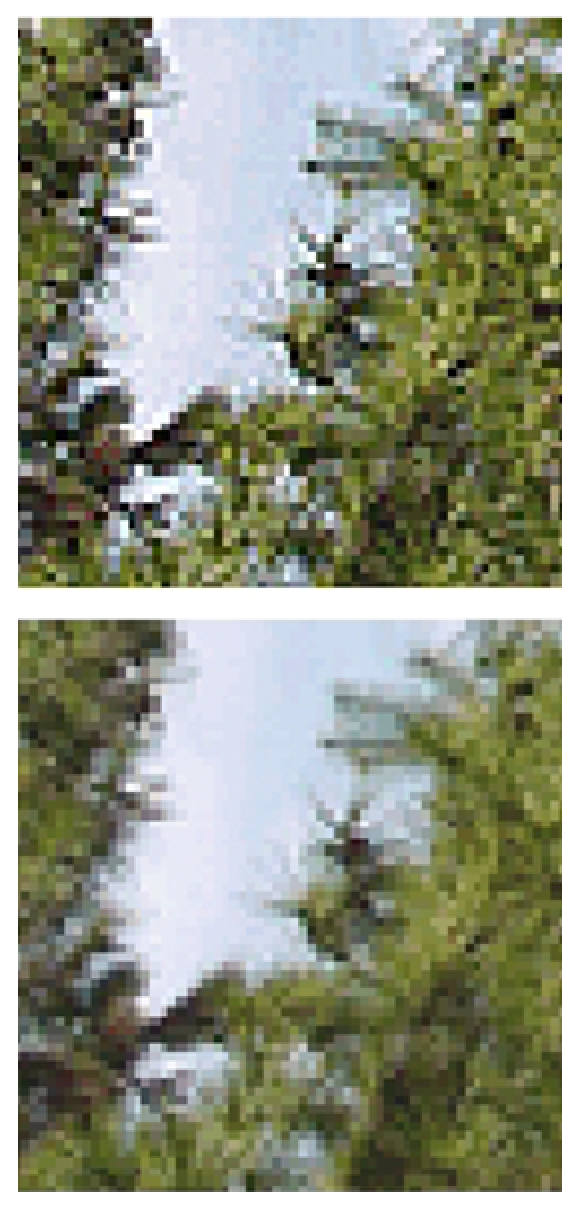
\includegraphics[angle=270,origin=b,width=0.75\textwidth]{unsharp.eps}
\caption{Unsharp}
\end{figure}

This is a 3x3 sharpening filter that emphasizes edges. By one burst operation, filter processing for 10 rows is performed for each of 6 locations (OMAP = 6) (RMGRP = 10). This is a stencil calculation therefore mapdist = 1.

\begin{screen}
\tiny
\begin{verbatim}
void unsharp(Uchar *p, Uchar *r)
#if !defined(EMAX5) && !defined(EMAX6)
  for (top=PAD; top<HT-PAD; top++) { /* scan-lines */
    Uchar *p0 = p+((top  )*WD+(0  ))*4;  // p1 p5 p2
    Uchar *p1 = p+((top-1)*WD+(0-1))*4;  // p6 p0 p7
    Uchar *p2 = p+((top-1)*WD+(0+1))*4;  // p3 p8 p4
    Uchar *p3 = p+((top+1)*WD+(0-1))*4;
    Uchar *p4 = p+((top+1)*WD+(0+1))*4;
    Uchar *p5 = p+((top-1)*WD+(0  ))*4;
    Uchar *p6 = p+((top  )*WD+(0-1))*4;
    Uchar *p7 = p+((top  )*WD+(0+1))*4;
    Uchar *p8 = p+((top+1)*WD+(0  ))*4;
    Uchar *rp = r+((top  )*WD+(0  ))*4;
    for (cofs=0; cofs<WD; cofs++) {
      int t0,t1,t2;
      rp[0] = 0;
      t0 = p0[1]; t1 = p1[1]+p2[1]+p3[1]+p4[1]; t2 = p5[1]+p6[1]+p7[1]+p8[1];
      rp[1] = limitRGB(( t0 * 239 - t1 * 13 - t2 * 15 - t2/4) >> 7);
      t0 = p0[2]; t1 = p1[2]+p2[2]+p3[2]+p4[2]; t2 = p5[2]+p6[2]+p7[2]+p8[2];
      rp[2] = limitRGB(( t0 * 239 - t1 * 13 - t2 * 15 - t2/4) >> 7);
      t0 = p0[3]; t1 = p1[3]+p2[3]+p3[3]+p4[3]; t2 = p5[3]+p6[3]+p7[3]+p8[3];
      rp[3] = limitRGB(( t0 * 239 - t1 * 13 - t2 * 15 - t2/4) >> 7);
      p0+=4; p1+=4; p2+=4; p3+=4; p4+=4; p5+=4; p6+=4; p7+=4; p8+=4; rp+=4;
    }
  }
#endif
\end{verbatim}
\end{screen}

\begin{screen}
\tiny
\begin{verbatim}
  for (top=0; top<RRANGE; top+=RMGRP) { /* scan-lines */
    for (rofs=0; rofs<RMGRP; rofs++) { /* will be parallelized by multi-chip (M/#chip) */
      for (CHIP=0; CHIP<NCHIP; CHIP++) { /* will be parallelized by multi-chip (M/#chip) */
        int idx = (CHIP*RRANGE*OMAP+top+rofs)*WD;
        Uchar *p0 = p+(idx   +(0  ))*4;  // p1 p5 p2
        Uchar *p1 = p+(idx-WD+(0-1))*4;  // p6 p0 p7
        Uchar *p2 = p+(idx-WD+(0+1))*4;  // p3 p8 p4
        Uchar *p3 = p+(idx+WD+(0-1))*4;
        Uchar *p4 = p+(idx+WD+(0+1))*4;
        Uchar *p5 = p+(idx-WD+(0  ))*4;
        Uchar *p6 = p+(idx   +(0-1))*4;
        Uchar *p7 = p+(idx   +(0+1))*4;
        Uchar *p8 = p+(idx+WD+(0  ))*4;
        Uchar *rp = r+(idx   +(0  ))*4;
        for (cofs=0; cofs<WD; cofs++) {
          for (oc=0; oc<OMAP; oc++) {
            Uint pix0 = (oc*RRANGE*WD+cofs)*4+0;
            Uint pix1 = (oc*RRANGE*WD+cofs)*4+1;
            Uint pix2 = (oc*RRANGE*WD+cofs)*4+2;
            Uint pix3 = (oc*RRANGE*WD+cofs)*4+3;
            int t0,t1,t2;
            rp[pix0] = 0;
            t0 = p0[pix1]; t1 = p1[pix1]+p2[pix1]+p3[pix1]+p4[pix1]; t2 = p5[pix1]+p6[pix1]+p7[pix1]+p8[pix1];
            rp[pix1] = limitRGB(( t0 * 239 - t1 * 13 - t2 * 15 - t2/4) >> 7);
            t0 = p0[pix2]; t1 = p1[pix2]+p2[pix2]+p3[pix2]+p4[pix2]; t2 = p5[pix2]+p6[pix2]+p7[pix2]+p8[pix2];
            rp[pix2] = limitRGB(( t0 * 239 - t1 * 13 - t2 * 15 - t2/4) >> 7);
            t0 = p0[pix3]; t1 = p1[pix3]+p2[pix3]+p3[pix3]+p4[pix3]; t2 = p5[pix3]+p6[pix3]+p7[pix3]+p8[pix3];
            rp[pix3] = limitRGB(( t0 * 239 - t1 * 13 - t2 * 15 - t2/4) >> 7);
          }
        }
      }
    }
  }
\end{verbatim}
\end{screen}

\begin{screen}
\tiny
\begin{verbatim}
  Ull  LOOP1, LOOP0;
  Ull  INIT1, INIT0;
  Ull  AR[64][4];                     /* output of EX     in each unit */
  Ull  BR[64][4][4];                  /* output registers in each unit */
  Ull  r0, r1, r2, r3, r4, r5, r6, r7, r8, r9, r10, r11, r12, r13, r14, r15;
  Ull  r16, r17, r18, r19, r20, r21, r22, r23, r24, r25, r26, r27, r28, r29, r30, r31;
  Ull  cc0, cc1, cc2, cc3, ex0, ex1;
  for (top=0; top<RRANGE; top+=RMGRP) { /* scan-lines */
    for (rofs=0; rofs<RMGRP; rofs++) { /* will be parallelized by multi-chip (M/#chip) */
      Uchar *pp0[NCHIP], *pc0[NCHIP], *pn0[NCHIP], *rc0[NCHIP];
      Uchar *pp1[NCHIP], *pc1[NCHIP], *pn1[NCHIP], *rc1[NCHIP];
      Uchar *pp2[NCHIP], *pc2[NCHIP], *pn2[NCHIP], *rc2[NCHIP];
      Uchar *pp3[NCHIP], *pc3[NCHIP], *pn3[NCHIP], *rc3[NCHIP];
      Uchar *pp4[NCHIP], *pc4[NCHIP], *pn4[NCHIP], *rc4[NCHIP];
      Uchar *pp5[NCHIP], *pc5[NCHIP], *pn5[NCHIP], *rc5[NCHIP];
      for (CHIP=0; CHIP<NCHIP; CHIP++) { /* will be parallelized by multi-chip (M/#chip) */
        int idx = (CHIP*RRANGE*OMAP+top+rofs)*WD*4;
        pp0[CHIP] = p+idx+RRANGE*WD* 0-1280;  pc0[CHIP] = p+idx+RRANGE*WD* 0; pn0[CHIP] = p+idx+RRANGE*WD* 0+1280; rc0[CHIP] = r+idx+RRANGE*WD* 0;
        pp1[CHIP] = p+idx+RRANGE*WD* 4-1280;  pc1[CHIP] = p+idx+RRANGE*WD* 4; pn1[CHIP] = p+idx+RRANGE*WD* 4+1280; rc1[CHIP] = r+idx+RRANGE*WD* 4;
        pp2[CHIP] = p+idx+RRANGE*WD* 8-1280;  pc2[CHIP] = p+idx+RRANGE*WD* 8; pn2[CHIP] = p+idx+RRANGE*WD* 8+1280; rc2[CHIP] = r+idx+RRANGE*WD* 8;
        pp3[CHIP] = p+idx+RRANGE*WD*12-1280;  pc3[CHIP] = p+idx+RRANGE*WD*12; pn3[CHIP] = p+idx+RRANGE*WD*12+1280; rc3[CHIP] = r+idx+RRANGE*WD*12;
        pp4[CHIP] = p+idx+RRANGE*WD*16-1280;  pc4[CHIP] = p+idx+RRANGE*WD*16; pn4[CHIP] = p+idx+RRANGE*WD*16+1280; rc4[CHIP] = r+idx+RRANGE*WD*16;
        pp5[CHIP] = p+idx+RRANGE*WD*20-1280;  pc5[CHIP] = p+idx+RRANGE*WD*20; pn5[CHIP] = p+idx+RRANGE*WD*20+1280; rc5[CHIP] = r+idx+RRANGE*WD*20;
      }
//EMAX5A begin unsharp mapdist=1
 /*2*/for (CHIP=0; CHIP<NCHIP; CHIP++) { /* output channels are parallelized by multi-chip (OC/#chip) */
   /*1*/for (INIT0=1,LOOP0=WD,cofs=0-4; LOOP0--; INIT0=0) {       /* stage#0 *//* mapped to FOR() on BR[63][0][0] */
 /*@0,1*/ exe(OP_ADD,       &cofs, cofs,      EXP_H3210, 4LL,  EXP_H3210, 0LL, EXP_H3210, OP_AND, 0x00000000ffffffffLL, OP_NOP, 0LL);
          /*map0*/
 /*@1,0*/ exe(OP_ADD,       &pofs, pc0[CHIP], EXP_H3210, cofs, EXP_H3210, 0LL, EXP_H3210, OP_NOP,  0LL,    OP_NOP,  0LL);
 /*@2,0*/ mop(OP_LDWR, 1,   &r1,   pofs,     -1276, MSK_D0,    (Ull)pp0[CHIP], WD,    0, 0, (Ull)NULL,   WD);
 /*@2,0*/ mop(OP_LDWR, 1,   &r2,   pofs,     -1284, MSK_D0,    (Ull)pp0[CHIP], WD,    0, 0, (Ull)NULL,   WD);
 /*@2,1*/ mop(OP_LDWR, 1,   &r5,   pofs,     -1280, MSK_D0,    (Ull)pp0[CHIP], WD,    0, 0, (Ull)NULL,   WD);
 /*@3,0*/ exe(OP_MAUH,      &r11,  r1,        EXP_B5410, r2,   EXP_B5410, 0LL, EXP_H3210, OP_NOP,  0LL,    OP_NOP,  0LL);
 /*@3,0*/ mop(OP_LDWR, 1,   &r6,   pofs,      4,    MSK_D0,    (Ull)pc0[CHIP], WD,    0, 0, (Ull)NULL,   WD);
 /*@3,0*/ mop(OP_LDWR, 1,   &r7,   pofs,     -4,    MSK_D0,    (Ull)pc0[CHIP], WD,    0, 0, (Ull)NULL,   WD);
 /*@3,1*/ exe(OP_MAUH,      &r12,  r1,        EXP_B7632, r2,   EXP_B7632, 0LL, EXP_H3210, OP_NOP,  0LL,    OP_NOP,  0LL);
 /*@3,1*/ mop(OP_LDWR, 1,   &r0,   pofs,      0,    MSK_D0,    (Ull)pc0[CHIP], WD,    0, 0, (Ull)NULL,   WD);
 /*@4,0*/ exe(OP_MLUH,      &r20,  r0,        EXP_B5410, 239,  EXP_H3210, 0LL, EXP_H3210, OP_NOP,  0LL,    OP_NOP,  0LL);
 /*@4,0*/ mop(OP_LDWR, 1,   &r3,   pofs,      1284, MSK_D0,    (Ull)pn0[CHIP], WD,    0, 0, (Ull)NULL,   WD);
 /*@4,0*/ mop(OP_LDWR, 1,   &r4,   pofs,      1276, MSK_D0,    (Ull)pn0[CHIP], WD,    0, 0, (Ull)NULL,   WD);
 /*@4,1*/ exe(OP_MLUH,      &r21,  r0,        EXP_B7632, 239,  EXP_H3210, 0LL, EXP_H3210, OP_NOP,  0LL,    OP_NOP,  0LL);
 /*@4,1*/ mop(OP_LDWR, 1,   &r8,   pofs,      1280, MSK_D0,    (Ull)pn0[CHIP], WD,    0, 0, (Ull)NULL,   WD);
 /*@4,2*/ exe(OP_MAUH,      &r15,  r5,        EXP_B5410, r6,   EXP_B5410, 0LL, EXP_H3210, OP_NOP,  0LL,    OP_NOP,  0LL);
 /*@4,3*/ exe(OP_MAUH,      &r16,  r5,        EXP_B7632, r6,   EXP_B7632, 0LL, EXP_H3210, OP_NOP,  0LL,    OP_NOP,  0LL);
 /*@5,0*/ exe(OP_MAUH3,     &r11,  r3,        EXP_B5410, r4,   EXP_B5410, r11, EXP_H3210, OP_NOP,  0LL,    OP_NOP,  0LL);
 /*@5,1*/ exe(OP_MAUH3,     &r12,  r3,        EXP_B7632, r4,   EXP_B7632, r12, EXP_H3210, OP_NOP,  0LL,    OP_NOP,  0LL);
 /*@6,0*/ exe(OP_MLUH,      &r13,  r11,       EXP_H3210, 13,   EXP_H3210, 0LL, EXP_H3210, OP_NOP,  0LL,    OP_NOP,  0LL);
 /*@6,1*/ exe(OP_MLUH,      &r14,  r12,       EXP_H3210, 13,   EXP_H3210, 0LL, EXP_H3210, OP_NOP,  0LL,    OP_NOP,  0LL);
 /*@6,2*/ exe(OP_MAUH3,     &r15,  r7,        EXP_B5410, r8,   EXP_B5410, r15, EXP_H3210, OP_NOP,  0LL,    OP_NOP,  0LL);
 /*@6,3*/ exe(OP_MAUH3,     &r16,  r7,        EXP_B7632, r8,   EXP_B7632, r16, EXP_H3210, OP_NOP,  0LL,    OP_NOP,  0LL);
 /*@7,0*/ exe(OP_NOP,       &r7,   r15,       EXP_H3210, 0LL,  EXP_H3210, 0LL, EXP_H3210, OP_OR,   0LL,    OP_SRLM, 2LL);
 /*@7,1*/ exe(OP_MLUH,      &r17,  r15,       EXP_H3210, 15,   EXP_H3210, 0LL, EXP_H3210, OP_NOP,  0LL,    OP_NOP,  0LL);
 /*@7,2*/ exe(OP_NOP,       &r8,   r16,       EXP_H3210, 0LL,  EXP_H3210, 0LL, EXP_H3210, OP_OR,   0LL,    OP_SRLM, 2LL);
 /*@7,3*/ exe(OP_MLUH,      &r18,  r16,       EXP_H3210, 15,   EXP_H3210, 0LL, EXP_H3210, OP_NOP,  0LL,    OP_NOP,  0LL);
 /*@8,0*/ exe(OP_MSUH3,     &r10,  r20,       EXP_H3210, r7,   EXP_H3210, r17, EXP_H3210, OP_NOP,  0LL,    OP_NOP,  0LL);
 /*@8,1*/ exe(OP_MSUH3,     &r11,  r21,       EXP_H3210, r8,   EXP_H3210, r18, EXP_H3210, OP_NOP,  0LL,    OP_NOP,  0LL);
 /*@9,0*/ exe(OP_MSUH,      &r20,  r10,       EXP_H3210, r13,  EXP_H3210, 0LL, EXP_H3210, OP_OR,   0LL,    OP_SRLM, 7LL);
 /*@9,1*/ exe(OP_MSUH,      &r21,  r11,       EXP_H3210, r14,  EXP_H3210, 0LL, EXP_H3210, OP_OR,   0LL,    OP_SRLM, 7LL);
 /*@10,0*/exe(OP_MH2BW,     &r31,  r21,       EXP_H3210, r20,  EXP_H3210, 0LL, EXP_H3210, OP_NOP,  0LL,    OP_NOP,  0LL);
 /*@10,0*/mop(OP_STWR, 3,   &r31,  rc0[CHIP], cofs, MSK_D0,    rc0[CHIP],      WD,    0, 0, (Ull)NULL,   WD);
       :
          /*map5*/
 /*@46,1*/exe(OP_ADD,       &pofs, pc5[CHIP], EXP_H3210, cofs, EXP_H3210, 0LL, EXP_H3210, OP_NOP,  0LL,    OP_NOP,  0LL);
 /*@47,0*/mop(OP_LDWR, 1,   &r1,   pofs,     -1276, MSK_D0,    (Ull)pp5[CHIP], WD,    0, 0, (Ull)NULL,   WD);
 /*@47,0*/mop(OP_LDWR, 1,   &r2,   pofs,     -1284, MSK_D0,    (Ull)pp5[CHIP], WD,    0, 0, (Ull)NULL,   WD);
 /*@47,1*/mop(OP_LDWR, 1,   &r5,   pofs,     -1280, MSK_D0,    (Ull)pp5[CHIP], WD,    0, 0, (Ull)NULL,   WD);
 /*@48,0*/exe(OP_MAUH,      &r11,  r1,        EXP_B5410, r2,   EXP_B5410, 0LL, EXP_H3210, OP_NOP,  0LL,    OP_NOP,  0LL);
 /*@48,0*/mop(OP_LDWR, 1,   &r6,   pofs,      4,    MSK_D0,    (Ull)pc5[CHIP], WD,    0, 0, (Ull)NULL,   WD);
 /*@48,0*/mop(OP_LDWR, 1,   &r7,   pofs,     -4,    MSK_D0,    (Ull)pc5[CHIP], WD,    0, 0, (Ull)NULL,   WD);
 /*@48,1*/exe(OP_MAUH,      &r12,  r1,        EXP_B7632, r2,   EXP_B7632, 0LL, EXP_H3210, OP_NOP,  0LL,    OP_NOP,  0LL);
 /*@48,1*/mop(OP_LDWR, 1,   &r0,   pofs,      0,    MSK_D0,    (Ull)pc5[CHIP], WD,    0, 0, (Ull)NULL,   WD);
 /*@49,0*/exe(OP_MLUH,      &r20,  r0,        EXP_B5410, 239,  EXP_H3210, 0LL, EXP_H3210, OP_NOP,  0LL,    OP_NOP,  0LL);
 /*@49,0*/mop(OP_LDWR, 1,   &r3,   pofs,      1284, MSK_D0,    (Ull)pn5[CHIP], WD,    0, 0, (Ull)NULL,   WD);
 /*@49,0*/mop(OP_LDWR, 1,   &r4,   pofs,      1276, MSK_D0,    (Ull)pn5[CHIP], WD,    0, 0, (Ull)NULL,   WD);
 /*@49,1*/exe(OP_MLUH,      &r21,  r0,        EXP_B7632, 239,  EXP_H3210, 0LL, EXP_H3210, OP_NOP,  0LL,    OP_NOP,  0LL);
 /*@49,1*/mop(OP_LDWR, 1,   &r8,   pofs,      1280, MSK_D0,    (Ull)pn5[CHIP], WD,    0, 0, (Ull)NULL,   WD);
 /*@49,2*/exe(OP_MAUH,      &r15,  r5,        EXP_B5410, r6,   EXP_B5410, 0LL, EXP_H3210, OP_NOP,  0LL,    OP_NOP,  0LL);
 /*@49,3*/exe(OP_MAUH,      &r16,  r5,        EXP_B7632, r6,   EXP_B7632, 0LL, EXP_H3210, OP_NOP,  0LL,    OP_NOP,  0LL);
 /*@50,0*/exe(OP_MAUH3,     &r11,  r3,        EXP_B5410, r4,   EXP_B5410, r11, EXP_H3210, OP_NOP,  0LL,    OP_NOP,  0LL);
 /*@50,1*/exe(OP_MAUH3,     &r12,  r3,        EXP_B7632, r4,   EXP_B7632, r12, EXP_H3210, OP_NOP,  0LL,    OP_NOP,  0LL);
 /*@51,0*/exe(OP_MLUH,      &r13,  r11,       EXP_H3210, 13,   EXP_H3210, 0LL, EXP_H3210, OP_NOP,  0LL,    OP_NOP,  0LL);
 /*@51,1*/exe(OP_MLUH,      &r14,  r12,       EXP_H3210, 13,   EXP_H3210, 0LL, EXP_H3210, OP_NOP,  0LL,    OP_NOP,  0LL);
 /*@51,2*/exe(OP_MAUH3,     &r15,  r7,        EXP_B5410, r8,   EXP_B5410, r15, EXP_H3210, OP_NOP,  0LL,    OP_NOP,  0LL);
 /*@51,3*/exe(OP_MAUH3,     &r16,  r7,        EXP_B7632, r8,   EXP_B7632, r16, EXP_H3210, OP_NOP,  0LL,    OP_NOP,  0LL);
 /*@52,0*/exe(OP_NOP,       &r7,   r15,       EXP_H3210, 0LL,  EXP_H3210, 0LL, EXP_H3210, OP_OR,   0LL,    OP_SRLM, 2LL);
 /*@52,1*/exe(OP_MLUH,      &r17,  r15,       EXP_H3210, 15,   EXP_H3210, 0LL, EXP_H3210, OP_NOP,  0LL,    OP_NOP,  0LL);
 /*@52,2*/exe(OP_NOP,       &r8,   r16,       EXP_H3210, 0LL,  EXP_H3210, 0LL, EXP_H3210, OP_OR,   0LL,    OP_SRLM, 2LL);
 /*@52,3*/exe(OP_MLUH,      &r18,  r16,       EXP_H3210, 15,   EXP_H3210, 0LL, EXP_H3210, OP_NOP,  0LL,    OP_NOP,  0LL);
 /*@53,0*/exe(OP_MSUH3,     &r10,  r20,       EXP_H3210, r7,   EXP_H3210, r17, EXP_H3210, OP_NOP,  0LL,    OP_NOP,  0LL);
 /*@53,1*/exe(OP_MSUH3,     &r11,  r21,       EXP_H3210, r8,   EXP_H3210, r18, EXP_H3210, OP_NOP,  0LL,    OP_NOP,  0LL);
 /*@54,0*/exe(OP_MSUH,      &r20,  r10,       EXP_H3210, r13,  EXP_H3210, 0LL, EXP_H3210, OP_OR,   0LL,    OP_SRLM, 7LL);
 /*@54,1*/exe(OP_MSUH,      &r21,  r11,       EXP_H3210, r14,  EXP_H3210, 0LL, EXP_H3210, OP_OR,   0LL,    OP_SRLM, 7LL);
 /*@55,0*/exe(OP_MH2BW,     &r31,  r21,       EXP_H3210, r20,  EXP_H3210, 0LL, EXP_H3210, OP_NOP,  0LL,    OP_NOP,  0LL);
 /*@55,0*/mop(OP_STWR, 3,   &r31,  rc5[CHIP], cofs, MSK_D0,    rc5[CHIP],      WD,    0, 0, (Ull)NULL,   WD);
        }
      }
//EMAX5A end
    }
  }
//EMAX5A drain_dirty_lmm
\end{verbatim}
\end{screen}

\begin{figure}[htbp]
\center
\epsfile{file=filter+rmm-unsharp-emax6.eps,width=1.00\textwidth}
\caption{Unsharp}
\end{figure}

\clearpage

\subsection{Blur with stencil}

\begin{figure}[htbp]
\center
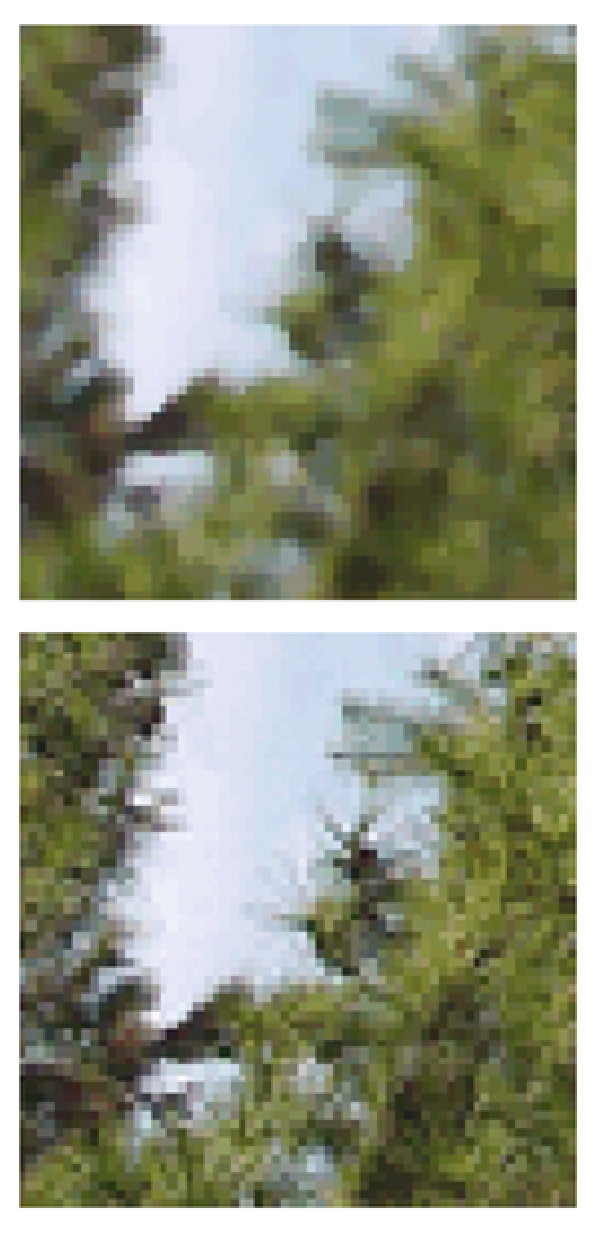
\includegraphics[angle=270,origin=b,width=0.55\textwidth]{blur.eps}
\caption{Blur}
\end{figure}

This is a 3x3 pipelined median filter. By one burst operation, 15 rows of filter processing are performed for each of the four locations (OMAP = 4) (RMGRP = 15). This is a stencil calculation with mapdist = 1.

\begin{screen}
\tiny
\begin{verbatim}
void blur(Uint *p, Uint *r)
#if !defined(EMAX5) && !defined(EMAX6)
  for (top=PAD; top<HT-PAD; top++) { /* scan-lines */
    Uint *p0 = p+(top  )*WD  ;
    Uint *p1 = p+(top  )*WD  ;
    Uint *p2 = p+(top  )*WD-1;
    Uint *p3 = p+(top  )*WD+1;
    Uint *p4 = p+(top-1)*WD  ;
    Uint *p5 = p+(top+1)*WD  ;
    Uint *p6 = p+(top-1)*WD-1;
    Uint *p7 = p+(top-1)*WD+1;
    Uint *p8 = p+(top+1)*WD-1;
    Uint *p9 = p+(top+1)*WD+1;
    Uint *rp = r+(top  )*WD  ;
    for (cofs=0; cofs<WD; cofs++) {
      *rp = (Uint)((*p1>>24&0xff)*20
          +  (*p2>>24&0xff)*12 + (*p3>>24&0xff)*12 + (*p4>>24&0xff)*12 + (*p5>>24&0xff)*12
          +  (*p6>>24&0xff)* 8 + (*p7>>24&0xff)* 8 + (*p8>>24&0xff)* 8 + (*p9>>24&0xff)* 8)/100<<24
          | (Uint)((*p1>>16&0xff)*20
          +  (*p2>>16&0xff)*12 + (*p3>>16&0xff)*12 + (*p4>>16&0xff)*12 + (*p5>>16&0xff)*12
          +  (*p6>>16&0xff)* 8 + (*p7>>16&0xff)* 8 + (*p8>>16&0xff)* 8 + (*p9>>16&0xff)* 8)/100<<16
          | (Uint)((*p1>> 8&0xff)*20
          +  (*p2>> 8&0xff)*12 + (*p3>> 8&0xff)*12 + (*p4>> 8&0xff)*12 + (*p5>> 8&0xff)*12
          +  (*p6>> 8&0xff)* 8 + (*p7>> 8&0xff)* 8 + (*p8>> 8&0xff)* 8 + (*p9>> 8&0xff)* 8)/100<<8;
      p0++; p1++; p2++; p3++; p4++; p5++; p6++; p7++; p8++; p9++; rp++;
    }
  }
#endif
\end{verbatim}
\end{screen}

\begin{screen}
\tiny
\begin{verbatim}
  for (top=PAD; top<HT-PAD; top++) { /* scan-lines */
    Uint *p0 = p+(top  )*WD  ;
    Uint *p1 = p+(top  )*WD  ;
    Uint *p2 = p+(top  )*WD-1;
    Uint *p3 = p+(top  )*WD+1;
    Uint *p4 = p+(top-1)*WD  ;
    Uint *p5 = p+(top+1)*WD  ;
    Uint *p6 = p+(top-1)*WD-1;
    Uint *p7 = p+(top-1)*WD+1;
    Uint *p8 = p+(top+1)*WD-1;
    Uint *p9 = p+(top+1)*WD+1;
    Uint *rp = r+(top  )*WD  ;
    for (cofs=0; cofs<WD; cofs++) {
      Uint s0,s1,s2,s3,s4,s5,s6,s7,s8;
      Uint t0,t1,t2;
      s0=*p1;s1=*p2;s2=*p3;s3=*p4;s4=*p5;s5=*p6;s6=*p7;s7=*p8;s8=*p9;
      /*��������������  ��������������  ��������������  ��������������  ��������������  ��������������  ������
        ��������������  �����㣳�����  ��������������  �����㣳�����  ������  ������  ������  �����  ������
        ���˨��˨��˨�  ��������������  ���˨��˨��˨�  ��������������  ���˨������˨�  ��������������  ���˨�
        ��������������  �����㣰�㣲��  ��������������  ��    ��    ��  ��  ��  ������  ��  ��  ������  ����������ͳ���
        ���˨��˨��˨�  ��������������  ���˨��˨��˨�  ��������������  ���˨������˨�  ��������������  ���˨�
        ��������������  �����㣴�㣸��  ��������������  �����㣴�㣸��  ������  ������  ������  �㣸��  ������
        ��������������  ��������������  ��������������  ��������������  ��������������  ��������������  ������*/
      t0 = pmax3(s5,s1,s7); t1 = pmid3(s5,s1,s7); t2 = pmin3(s5,s1,s7);      s5 = t0; s1 = t1; s7 = t2;
      t0 = pmax3(s3,s0,s4); t1 = pmid3(s3,s0,s4); t2 = pmin3(s3,s0,s4);      s3 = t0; s0 = t1; s4 = t2;
      t0 = pmax3(s6,s2,s8); t1 = pmid3(s6,s2,s8); t2 = pmin3(s6,s2,s8);      s6 = t0; s2 = t1; s8 = t2;

      t0 = pmin3(s5,s3,s6); t1 = pmid3(s5,s3,s6);                            s5 = t0; s3 = t1;
      t0 = pmin3(s1,s0,s2); t1 = pmid3(s1,s0,s2); t2 = pmax3(s1,s0,s2);      s1 = t0; s0 = t1; s2 = t2;
      t0 = pmid3(s7,s4,s8); t1 = pmax3(s7,s4,s8);                            s4 = t0; s8 = t1;

      t0 = pmax2(s5,s1);    t1 = pmin2(s5,s1);                               s5 = t0; s1 = t1;
      t0 = pmax3(s3,s0,s4); t1 = pmid3(s3,s0,s4); t2 = pmin3(s3,s0,s4);      s3 = t0; s0 = t1; s4 = t2;
      t0 = pmax2(s2,s8);    t1 = pmin2(s2,s8);                               s2 = t0; s8 = t1;

      t0 = pmin3(s5,s3,s2); t1 = pmid3(s5,s3,s2);                            s5 = t0; s3 = t1;
      t0 = pmid3(s1,s4,s8); t1 = pmax3(s1,s4,s8);                            s4 = t0; s8 = t1;

      t0 = pmax2(s5,s4);    t1 = pmin2(s5,s4);                               s5 = t0; s4 = t1;
      t0 = pmax3(s3,s0,s8); t1 = pmid3(s3,s0,s8); t2 = pmin3(s3,s0,s8);      s3 = t0; s0 = t1; s8 = t2;

      s5 = pmin2(s5,s3);    s8 = pmax2(s4,s8);

      *rp = pmid3(s5,s0,s8);
      p0++; p1++; p2++; p3++; p4++; p5++; p6++; p7++; p8++; p9++; rp++;
    }
  }
\end{verbatim}
\end{screen}

\begin{screen}
\tiny
\begin{verbatim}
  Ull  LOOP1, LOOP0;
  Ull  INIT1, INIT0;
  Ull  AR[64][4];                     /* output of EX     in each unit */
  Ull  BR[64][4][4];                  /* output registers in each unit */
  Ull  r0, r1, r2, r3, r4, r5, r6, r7, r8, r9, r10, r11, r12, r13, r14, r15;
  Ull  r16, r17, r18, r19, r20, r21, r22, r23, r24, r25, r26, r27, r28, r29, r30, r31;
  Ull  cc0, cc1, cc2, cc3, ex0, ex1;
  for (top=0; top<RRANGE; top+=RMGRP) { /* scan-lines */
    for (rofs=0; rofs<RMGRP; rofs++) { /* will be parallelized by multi-chip (M/#chip) */
      Uint *pp0[NCHIP], *pc0[NCHIP], *pn0[NCHIP], *rc0[NCHIP];
      Uint *pp1[NCHIP], *pc1[NCHIP], *pn1[NCHIP], *rc1[NCHIP];
      Uint *pp2[NCHIP], *pc2[NCHIP], *pn2[NCHIP], *rc2[NCHIP];
      Uint *pp3[NCHIP], *pc3[NCHIP], *pn3[NCHIP], *rc3[NCHIP];
      for (CHIP=0; CHIP<NCHIP; CHIP++) { /* will be parallelized by multi-chip (M/#chip) */
        int idx = (CHIP*RRANGE*OMAP+top+rofs)*WD;
        pp0[CHIP] = p+idx+RRANGE*WD*0-WD;  pc0[CHIP] = p+idx+RRANGE*WD*0; pn0[CHIP] = p+idx+RRANGE*WD*0+WD; rc0[CHIP] = r+idx+RRANGE*WD*0;
        pp1[CHIP] = p+idx+RRANGE*WD*1-WD;  pc1[CHIP] = p+idx+RRANGE*WD*1; pn1[CHIP] = p+idx+RRANGE*WD*1+WD; rc1[CHIP] = r+idx+RRANGE*WD*1;
        pp2[CHIP] = p+idx+RRANGE*WD*2-WD;  pc2[CHIP] = p+idx+RRANGE*WD*2; pn2[CHIP] = p+idx+RRANGE*WD*2+WD; rc2[CHIP] = r+idx+RRANGE*WD*2;
        pp3[CHIP] = p+idx+RRANGE*WD*3-WD;  pc3[CHIP] = p+idx+RRANGE*WD*3; pn3[CHIP] = p+idx+RRANGE*WD*3+WD; rc3[CHIP] = r+idx+RRANGE*WD*3;
      }
//EMAX5A begin blur mapdist=1
 /*2*/for (CHIP=0; CHIP<NCHIP; CHIP++) { /* output channels are parallelized by multi-chip (OC/#chip) */
   /*1*/for (INIT0=1,LOOP0=WD,cofs=0-4; LOOP0--; INIT0=0) {       /* stage#0 *//* mapped to FOR() on BR[63][0][0] */
 /*@0,1*/ exe(OP_ADD,       &cofs, cofs,      EXP_H3210, 4LL,  EXP_H3210, 0LL, EXP_H3210, OP_AND, 0x00000000ffffffffLL, OP_NOP, 0LL);
          /*map0*/
 /*@1,0*/ exe(OP_ADD,       &pofs, pc0[CHIP], EXP_H3210, cofs, EXP_H3210, 0LL, EXP_H3210, OP_NOP,  0LL,    OP_NOP,  0LL);
 /*@2,0*/ mop(OP_LDWR, 1,   &r7,   pofs,     -1276, MSK_D0,    pp0[CHIP],      WD,   0, 0, (Ull)NULL,    WD);
 /*@2,0*/ mop(OP_LDWR, 1,   &r1,   pofs,     -1280, MSK_D0,    pp0[CHIP],      WD,   0, 0, (Ull)NULL,    WD);
 /*@2,1*/ mop(OP_LDWR, 1,   &r5,   pofs,     -1284, MSK_D0,    pp0[CHIP],      WD,   0, 0, (Ull)NULL,    WD);
 /*@3,0*/ exe(OP_MMIN3,     &r17,  r7,        EXP_H3210, r1,   EXP_H3210, r5,  EXP_H3210, OP_NOP,  0LL,    OP_NOP,  0LL);
 /*@3,0*/ mop(OP_LDWR, 1,   &r4,   pofs,         4, MSK_D0,    pc0[CHIP],      WD,   0, 0, (Ull)NULL,    WD);
 /*@3,0*/ mop(OP_LDWR, 1,   &r0,   pofs,         0, MSK_D0,    pc0[CHIP],      WD,   0, 0, (Ull)NULL,    WD);
 /*@3,1*/ exe(OP_MMID3,     &r11,  r7,        EXP_H3210, r1,   EXP_H3210, r5,  EXP_H3210, OP_NOP,  0LL,    OP_NOP,  0LL);
 /*@3,1*/ mop(OP_LDWR, 1,   &r3,   pofs,        -4, MSK_D0,    pc0[CHIP],      WD,   0, 0, (Ull)NULL,    WD);
 /*@3,2*/ exe(OP_MMAX3,     &r15,  r7,        EXP_H3210, r1,   EXP_H3210, r5,  EXP_H3210, OP_NOP,  0LL,    OP_NOP,  0LL);
 /*@4,0*/ exe(OP_MMIN3,     &r14,  r4,        EXP_H3210, r0,   EXP_H3210, r3,  EXP_H3210, OP_NOP,  0LL,    OP_NOP,  0LL);
 /*@4,0*/ mop(OP_LDWR, 1,   &r8,   pofs,      1284, MSK_D0,    pn0[CHIP],      WD,   0, 0, (Ull)NULL,    WD);
 /*@4,0*/ mop(OP_LDWR, 1,   &r2,   pofs,      1280, MSK_D0,    pn0[CHIP],      WD,   0, 0, (Ull)NULL,    WD);
 /*@4,1*/ exe(OP_MMID3,     &r10,  r4,        EXP_H3210, r0,   EXP_H3210, r3,  EXP_H3210, OP_NOP,  0LL,    OP_NOP,  0LL);
 /*@4,1*/ mop(OP_LDWR, 1,   &r6,   pofs,      1276, MSK_D0,    pn0[CHIP],      WD,   0, 0, (Ull)NULL,    WD);
 /*@4,2*/ exe(OP_MMAX3,     &r13,  r4,        EXP_H3210, r0,   EXP_H3210, r3,  EXP_H3210, OP_NOP,  0LL,    OP_NOP,  0LL);
 /*@5,0*/ exe(OP_MMIN3,     &r18,  r8,        EXP_H3210, r2,   EXP_H3210, r6,  EXP_H3210, OP_NOP,  0LL,    OP_NOP,  0LL);
 /*@5,1*/ exe(OP_MMID3,     &r12,  r8,        EXP_H3210, r2,   EXP_H3210, r6,  EXP_H3210, OP_NOP,  0LL,    OP_NOP,  0LL);
 /*@5,2*/ exe(OP_MMAX3,     &r16,  r8,        EXP_H3210, r2,   EXP_H3210, r6,  EXP_H3210, OP_NOP,  0LL,    OP_NOP,  0LL);
 /*step-2*/
 /*@6,0*/ exe(OP_MMAX3,     &r2,   r11,       EXP_H3210, r10,  EXP_H3210, r12, EXP_H3210, OP_NOP,  0LL,    OP_NOP,  0LL);
 /*@6,1*/ exe(OP_MMID3,     &r0,   r11,       EXP_H3210, r10,  EXP_H3210, r12, EXP_H3210, OP_NOP,  0LL,    OP_NOP,  0LL);
 /*@6,2*/ exe(OP_MMIN3,     &r1,   r11,       EXP_H3210, r10,  EXP_H3210, r12, EXP_H3210, OP_NOP,  0LL,    OP_NOP,  0LL);
 /*@6,3*/ exe(OP_MMAX3,     &r8,   r17,       EXP_H3210, r14,  EXP_H3210, r18, EXP_H3210, OP_NOP,  0LL,    OP_NOP,  0LL);
 /*@7,0*/ exe(OP_MMID3,     &r4,   r17,       EXP_H3210, r14,  EXP_H3210, r18, EXP_H3210, OP_NOP,  0LL,    OP_NOP,  0LL);
 /*@7,1*/ exe(OP_MMID3,     &r3,   r15,       EXP_H3210, r13,  EXP_H3210, r16, EXP_H3210, OP_NOP,  0LL,    OP_NOP,  0LL);
 /*@7,2*/ exe(OP_MMIN3,     &r5,   r15,       EXP_H3210, r13,  EXP_H3210, r16, EXP_H3210, OP_NOP,  0LL,    OP_NOP,  0LL);
 /*step-3*/
 /*@8,0*/ exe(OP_MMIN3,     &r14,  r3,        EXP_H3210, r0,   EXP_H3210, r4,  EXP_H3210, OP_NOP,  0LL,    OP_NOP,  0LL);
 /*@8,1*/ exe(OP_MMID3,     &r10,  r3,        EXP_H3210, r0,   EXP_H3210, r4,  EXP_H3210, OP_NOP,  0LL,    OP_NOP,  0LL);
 /*@8,2*/ exe(OP_MMAX3,     &r13,  r3,        EXP_H3210, r0,   EXP_H3210, r4,  EXP_H3210, OP_NOP,  0LL,    OP_NOP,  0LL);
 /*@8,3*/ exe(OP_MMIN,      &r18,  r2,        EXP_H3210, r8,   EXP_H3210, 0LL, EXP_H3210, OP_NOP,  0LL,    OP_NOP,  0LL);
 /*@9,0*/ exe(OP_MMAX,      &r12,  r2,        EXP_H3210, r8,   EXP_H3210, 0LL, EXP_H3210, OP_NOP,  0LL,    OP_NOP,  0LL);
 /*@9,1*/ exe(OP_MMIN,      &r11,  r5,        EXP_H3210, r1,   EXP_H3210, 0LL, EXP_H3210, OP_NOP,  0LL,    OP_NOP,  0LL);
 /*@9,2*/ exe(OP_MMAX,      &r15,  r5,        EXP_H3210, r1,   EXP_H3210, 0LL, EXP_H3210, OP_NOP,  0LL,    OP_NOP,  0LL);
 /*step-4*/
 /*@10,0*/exe(OP_MMID3,     &r4,   r11,       EXP_H3210, r14,  EXP_H3210, r18, EXP_H3210, OP_NOP,  0LL,    OP_NOP,  0LL);
 /*@10,1*/exe(OP_MMIN3,     &r5,   r15,       EXP_H3210, r13,  EXP_H3210, r12, EXP_H3210, OP_NOP,  0LL,    OP_NOP,  0LL);
 /*step-5*/
 /*@10,2*/exe(OP_MMAX3,     &r8,   r11,       EXP_H3210, r14,  EXP_H3210, r18, EXP_H3210, OP_NOP,  0LL,    OP_NOP,  0LL);
 /*@10,3*/exe(OP_MMID3,     &r3,   r15,       EXP_H3210, r13,  EXP_H3210, r12, EXP_H3210, OP_NOP,  0LL,    OP_NOP,  0LL);
 /*@11,0*/exe(OP_MMIN,      &r14,  r5,        EXP_H3210, r4,   EXP_H3210, 0LL, EXP_H3210, OP_NOP,  0LL,    OP_NOP,  0LL);
 /*@11,1*/exe(OP_MMAX,      &r15,  r5,        EXP_H3210, r4,   EXP_H3210, 0LL, EXP_H3210, OP_NOP,  0LL,    OP_NOP,  0LL);
 /*@11,2*/exe(OP_MMIN3,     &r18,  r3,        EXP_H3210, r10,  EXP_H3210, r8,  EXP_H3210, OP_NOP,  0LL,    OP_NOP,  0LL);
 /*@11,3*/exe(OP_MMID3,     &r10,  r3,        EXP_H3210, r10,  EXP_H3210, r8,  EXP_H3210, OP_NOP,  0LL,    OP_NOP,  0LL);
 /*@12,0*/exe(OP_MMAX3,     &r13,  r3,        EXP_H3210, r10,  EXP_H3210, r8,  EXP_H3210, OP_NOP,  0LL,    OP_NOP,  0LL);
 /*step-6*/
 /*@12,1*/exe(OP_MMAX,      &r8,   r14,       EXP_H3210, r18,  EXP_H3210, 0LL, EXP_H3210, OP_NOP,  0LL,    OP_NOP,  0LL);
 /*@13,0*/exe(OP_MMIN,      &r5,   r15,       EXP_H3210, r13,  EXP_H3210, 0LL, EXP_H3210, OP_NOP,  0LL,    OP_NOP,  0LL);
 /*@14,0*/exe(OP_MMID3,     &r31,  r5,        EXP_H3210, r10,  EXP_H3210, r8,  EXP_H3210, OP_NOP,  0LL,    OP_NOP,  0LL);
 /*@14,0*/mop(OP_STWR, 3,   &r31,  rc0[CHIP], cofs, MSK_D0,    rc0[CHIP],      WD,   0, 0, (Ull)NULL,    WD);
     :
          /*map3*/
 /*@40,1*/exe(OP_ADD,       &pofs, pc3[CHIP], EXP_H3210, cofs, EXP_H3210, 0LL, EXP_H3210, OP_NOP,  0LL,    OP_NOP,  0LL);
 /*@41,0*/mop(OP_LDWR, 1,   &r7,   pofs,     -1276, MSK_D0,    pp3[CHIP],      WD,   0, 0, (Ull)NULL,    WD);
 /*@41,0*/mop(OP_LDWR, 1,   &r1,   pofs,     -1280, MSK_D0,    pp3[CHIP],      WD,   0, 0, (Ull)NULL,    WD);
 /*@41,1*/mop(OP_LDWR, 1,   &r5,   pofs,     -1284, MSK_D0,    pp3[CHIP],      WD,   0, 0, (Ull)NULL,    WD);
 /*@42,0*/exe(OP_MMIN3,     &r17,  r7,        EXP_H3210, r1,   EXP_H3210, r5,  EXP_H3210, OP_NOP,  0LL,    OP_NOP,  0LL);
 /*@42,0*/mop(OP_LDWR, 1,   &r4,   pofs,         4, MSK_D0,    pc3[CHIP],      WD,   0, 0, (Ull)NULL,    WD);
 /*@42,0*/mop(OP_LDWR, 1,   &r0,   pofs,         0, MSK_D0,    pc3[CHIP],      WD,   0, 0, (Ull)NULL,    WD);
 /*@42,1*/exe(OP_MMID3,     &r11,  r7,        EXP_H3210, r1,   EXP_H3210, r5,  EXP_H3210, OP_NOP,  0LL,    OP_NOP,  0LL);
 /*@42,1*/mop(OP_LDWR, 1,   &r3,   pofs,        -4, MSK_D0,    pc3[CHIP],      WD,   0, 0, (Ull)NULL,    WD);
 /*@42,2*/exe(OP_MMAX3,     &r15,  r7,        EXP_H3210, r1,   EXP_H3210, r5,  EXP_H3210, OP_NOP,  0LL,    OP_NOP,  0LL);
 /*@43,0*/exe(OP_MMIN3,     &r14,  r4,        EXP_H3210, r0,   EXP_H3210, r3,  EXP_H3210, OP_NOP,  0LL,    OP_NOP,  0LL);
 /*@43,0*/mop(OP_LDWR, 1,   &r8,   pofs,      1284, MSK_D0,    pn3[CHIP],      WD,   0, 0, (Ull)NULL,    WD);
 /*@43,0*/mop(OP_LDWR, 1,   &r2,   pofs,      1280, MSK_D0,    pn3[CHIP],      WD,   0, 0, (Ull)NULL,    WD);
 /*@43,1*/exe(OP_MMID3,     &r10,  r4,        EXP_H3210, r0,   EXP_H3210, r3,  EXP_H3210, OP_NOP,  0LL,    OP_NOP,  0LL);
 /*@43,1*/mop(OP_LDWR, 1,   &r6,   pofs,      1276, MSK_D0,    pn3[CHIP],      WD,   0, 0, (Ull)NULL,    WD);
 /*@43,2*/exe(OP_MMAX3,     &r13,  r4,        EXP_H3210, r0,   EXP_H3210, r3,  EXP_H3210, OP_NOP,  0LL,    OP_NOP,  0LL);
 /*@44,0*/exe(OP_MMIN3,     &r18,  r8,        EXP_H3210, r2,   EXP_H3210, r6,  EXP_H3210, OP_NOP,  0LL,    OP_NOP,  0LL);
 /*@44,1*/exe(OP_MMID3,     &r12,  r8,        EXP_H3210, r2,   EXP_H3210, r6,  EXP_H3210, OP_NOP,  0LL,    OP_NOP,  0LL);
 /*@44,2*/exe(OP_MMAX3,     &r16,  r8,        EXP_H3210, r2,   EXP_H3210, r6,  EXP_H3210, OP_NOP,  0LL,    OP_NOP,  0LL);
 /*step-2*/
    :
 /*step-5*/
 /*@49,2*/exe(OP_MMAX3,     &r8,   r11,       EXP_H3210, r14,  EXP_H3210, r18, EXP_H3210, OP_NOP,  0LL,    OP_NOP,  0LL);
 /*@49,3*/exe(OP_MMID3,     &r3,   r15,       EXP_H3210, r13,  EXP_H3210, r12, EXP_H3210, OP_NOP,  0LL,    OP_NOP,  0LL);
 /*@50,0*/exe(OP_MMIN,      &r14,  r5,        EXP_H3210, r4,   EXP_H3210, 0LL, EXP_H3210, OP_NOP,  0LL,    OP_NOP,  0LL);
 /*@50,1*/exe(OP_MMAX,      &r15,  r5,        EXP_H3210, r4,   EXP_H3210, 0LL, EXP_H3210, OP_NOP,  0LL,    OP_NOP,  0LL);
 /*@50,2*/exe(OP_MMIN3,     &r18,  r3,        EXP_H3210, r10,  EXP_H3210, r8,  EXP_H3210, OP_NOP,  0LL,    OP_NOP,  0LL);
 /*@50,3*/exe(OP_MMID3,     &r10,  r3,        EXP_H3210, r10,  EXP_H3210, r8,  EXP_H3210, OP_NOP,  0LL,    OP_NOP,  0LL);
 /*@51,0*/exe(OP_MMAX3,     &r13,  r3,        EXP_H3210, r10,  EXP_H3210, r8,  EXP_H3210, OP_NOP,  0LL,    OP_NOP,  0LL);
 /*step-6*/
 /*@51,1*/exe(OP_MMAX,      &r8,   r14,       EXP_H3210, r18,  EXP_H3210, 0LL, EXP_H3210, OP_NOP,  0LL,    OP_NOP,  0LL);
 /*@52,0*/exe(OP_MMIN,      &r5,   r15,       EXP_H3210, r13,  EXP_H3210, 0LL, EXP_H3210, OP_NOP,  0LL,    OP_NOP,  0LL);
 /*@53,0*/exe(OP_MMID3,     &r31,  r5,        EXP_H3210, r10,  EXP_H3210, r8,  EXP_H3210, OP_NOP,  0LL,    OP_NOP,  0LL);
 /*@53,0*/mop(OP_STWR, 3,   &r31,  rc3[CHIP], cofs, MSK_D0,    rc3[CHIP],      WD,   0, 0, (Ull)NULL,    WD);
        }
      }
//EMAX5A end
    }
  }
//EMAX5A drain_dirty_lmm
\end{verbatim}
\end{screen}

\begin{figure}[htbp]
\center
\epsfile{file=filter+rmm-blur-emax6.eps,width=1.00\textwidth}
\caption{Blur}
\end{figure}

\clearpage

\subsection{Edge with stencil}

\begin{figure}[htbp]
\center
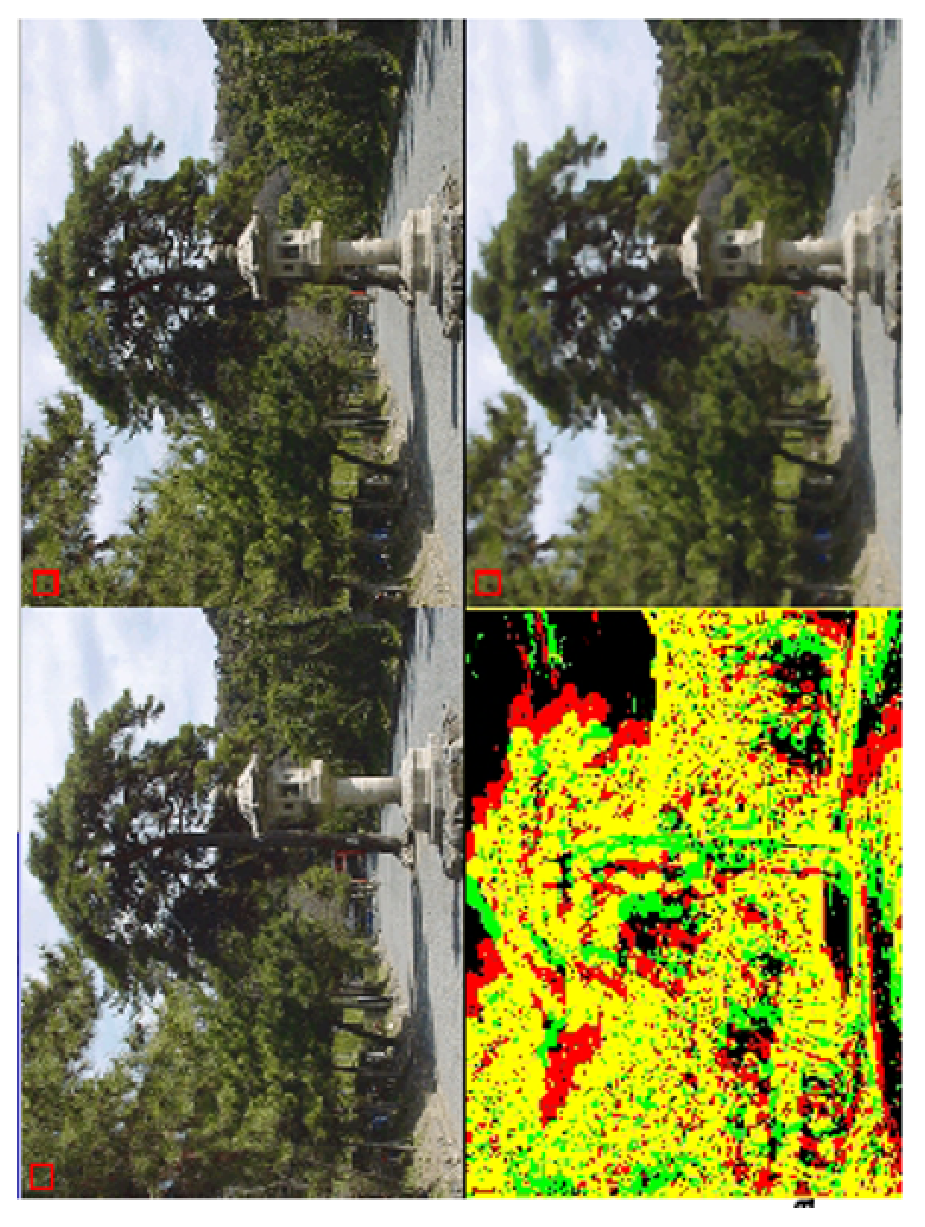
\includegraphics[angle=270,origin=b,width=0.75\textwidth]{edge.eps}
\caption{Edge}
\end{figure}

This is a 3x3 edge detection filter. By one burst operation, filter processing for 10 rows is performed for each of 6 locations (OMAP = 6) (RMGRP = 10). This is a stencil calculation with mapdist = 1.

\begin{screen}
\tiny
\begin{verbatim}
void edge(Uint *p, struct E *r)
#if !defined(EMAX5) && !defined(EMAX6)
  for (top=PAD; top<HT-PAD; top++) { /* scan-lines */
    Uint  *p0 = p+(top  )*WD  ;
    Uint  *p1 = p+(top-1)*WD-1;
    Uint  *p2 = p+(top+1)*WD+1;
    Uint  *p3 = p+(top-1)*WD  ;
    Uint  *p4 = p+(top+1)*WD  ;
    Uint  *p5 = p+(top-1)*WD+1;
    Uint  *p6 = p+(top+1)*WD-1;
    Uint  *p7 = p+(top  )*WD-1;
    Uint  *p8 = p+(top  )*WD+1;
    Uchar *rp = r->E[top];
    for (cofs=0; cofs<WD; cofs++) {
      int d1 = df(*p1&MASK,*p2&MASK)+df(*p3&MASK,*p4&MASK)+df(*p5&MASK,*p6&MASK)+df(*p7&MASK,*p8&MASK);
      /* 0 < d1(42) < 256*2*4 */
      *rp = d1 < EDGEDET ? 0 : PIXMAX;
      p0++; p1++; p2++; p3++; p4++; p5++; p6++; p7++; p8++; rp++;
    }
  }
#endif
\end{verbatim}
\end{screen}

\begin{screen}
\tiny
\begin{verbatim}
  Ull  LOOP1, LOOP0;
  Ull  INIT1, INIT0;
  Ull  AR[64][4];                     /* output of EX     in each unit */
  Ull  BR[64][4][4];                  /* output registers in each unit */
  Ull  r0, r1, r2, r3, r4, r5, r6, r7, r8, r9, r10, r11, r12, r13, r14, r15;
  Ull  r16, r17, r18, r19, r20, r21, r22, r23, r24, r25, r26, r27, r28, r29, r30, r31;
  Ull  cc0, cc1, cc2, cc3, ex0, ex1;
  for (top=0; top<RRANGE; top+=RMGRP) { /* scan-lines */
    for (rofs=0; rofs<RMGRP; rofs++) { /* will be parallelized by multi-chip (M/#chip) */
      Uint *pp0[NCHIP], *pc0[NCHIP], *pn0[NCHIP]; Uchar *rc0[NCHIP];
      Uint *pp1[NCHIP], *pc1[NCHIP], *pn1[NCHIP]; Uchar *rc1[NCHIP];
      Uint *pp2[NCHIP], *pc2[NCHIP], *pn2[NCHIP]; Uchar *rc2[NCHIP];
      Uint *pp3[NCHIP], *pc3[NCHIP], *pn3[NCHIP]; Uchar *rc3[NCHIP];
      Uint *pp4[NCHIP], *pc4[NCHIP], *pn4[NCHIP]; Uchar *rc4[NCHIP];
      Uint *pp5[NCHIP], *pc5[NCHIP], *pn5[NCHIP]; Uchar *rc5[NCHIP];
      for (CHIP=0; CHIP<NCHIP; CHIP++) { /* will be parallelized by multi-chip (M/#chip) */
        int idx = (CHIP*RRANGE*OMAP+top+rofs)*WD;
        pp0[CHIP] = p+idx+RRANGE*WD*0-WD;  pc0[CHIP] = p+idx+RRANGE*WD*0; pn0[CHIP] = p+idx+RRANGE*WD*0+WD; rc0[CHIP] = (Uchar*)(r->E)+idx+RRANGE*WD*0;
        pp1[CHIP] = p+idx+RRANGE*WD*1-WD;  pc1[CHIP] = p+idx+RRANGE*WD*1; pn1[CHIP] = p+idx+RRANGE*WD*1+WD; rc1[CHIP] = (Uchar*)(r->E)+idx+RRANGE*WD*1;
        pp2[CHIP] = p+idx+RRANGE*WD*2-WD;  pc2[CHIP] = p+idx+RRANGE*WD*2; pn2[CHIP] = p+idx+RRANGE*WD*2+WD; rc2[CHIP] = (Uchar*)(r->E)+idx+RRANGE*WD*2;
        pp3[CHIP] = p+idx+RRANGE*WD*3-WD;  pc3[CHIP] = p+idx+RRANGE*WD*3; pn3[CHIP] = p+idx+RRANGE*WD*3+WD; rc3[CHIP] = (Uchar*)(r->E)+idx+RRANGE*WD*3;
        pp4[CHIP] = p+idx+RRANGE*WD*4-WD;  pc4[CHIP] = p+idx+RRANGE*WD*4; pn4[CHIP] = p+idx+RRANGE*WD*4+WD; rc4[CHIP] = (Uchar*)(r->E)+idx+RRANGE*WD*4;
        pp5[CHIP] = p+idx+RRANGE*WD*5-WD;  pc5[CHIP] = p+idx+RRANGE*WD*5; pn5[CHIP] = p+idx+RRANGE*WD*5+WD; rc5[CHIP] = (Uchar*)(r->E)+idx+RRANGE*WD*5;
      }
//EMAX5A begin edge mapdist=1
 /*2*/for (CHIP=0; CHIP<NCHIP; CHIP++) { /* output channels are parallelized by multi-chip (OC/#chip) */
   /*1*/for (INIT0=1,LOOP0=WD,cofs=0-4; LOOP0--; INIT0=0) {       /* stage#0 *//* mapped to FOR() on BR[63][0][0] */
 /*@0,1*/ exe(OP_ADD,       &cofs, cofs,        EXP_H3210, 4LL,  EXP_H3210, 0LL, EXP_H3210, OP_AND, 0x00000000ffffffffLL, OP_NOP, 0LL);
          /*map0*/
 /*@1,0*/ exe(OP_ADD,       &pofs, pc0[CHIP],   EXP_H3210, cofs, EXP_H3210, 0LL, EXP_H3210, OP_NOP,   0LL,    OP_NOP,  0LL);
 /*@2,0*/ mop(OP_LDWR, 1,   &r5,   pofs,       -1276, MSK_D0,    (Ull)pp0[CHIP],       WD,     0,   0,   (Ull)NULL,  WD);
 /*@2,0*/ mop(OP_LDWR, 1,   &r3,   pofs,       -1280, MSK_D0,    (Ull)pp0[CHIP],       WD,     0,   0,   (Ull)NULL,  WD);
 /*@2,1*/ mop(OP_LDWR, 1,   &r1,   pofs,       -1284, MSK_D0,    (Ull)pp0[CHIP],       WD,     0,   0,   (Ull)NULL,  WD);
 /*@3,0*/ exe(OP_NOP,    &AR[3][0],0LL,         EXP_H3210, 0LL,  EXP_H3210, 0LL, EXP_H3210, OP_OR,    0LL,    OP_NOP,  0LL);
 /*@3,0*/ mop(OP_LDWR, 1,   &r8,   pofs,           4, MSK_D0,    (Ull)pc0[CHIP],       WD,     0,   0,   (Ull)NULL,  WD);
 /*@3,0*/ mop(OP_LDWR, 1,   &r7,   pofs,          -4, MSK_D0,    (Ull)pc0[CHIP],       WD,     0,   0,   (Ull)NULL,  WD);
 /*@4,0*/ exe(OP_NOP,    &AR[4][0],0LL,         EXP_H3210, 0LL,  EXP_H3210, 0LL, EXP_H3210, OP_OR,    0LL,    OP_NOP,  0LL);
 /*@4,0*/ mop(OP_LDWR, 1,   &r2,   pofs,        1284, MSK_D0,    (Ull)pn0[CHIP],       WD,     0,   0,   (Ull)NULL,  WD);
 /*@4,0*/ mop(OP_LDWR, 1,   &r4,   pofs,        1280, MSK_D0,    (Ull)pn0[CHIP],       WD,     0,   0,   (Ull)NULL,  WD);
 /*@4,1*/ mop(OP_LDWR, 1,   &r6,   pofs,        1276, MSK_D0,    (Ull)pn0[CHIP],       WD,     0,   0,   (Ull)NULL,  WD);
 /*@4,1*/ exe(OP_MSSAD,     &r7,   0LL,         EXP_H3210, r7,   EXP_H3210, r8,  EXP_H3210, OP_NOP,   0LL,    OP_NOP,  0LL);
 /*@5,0*/ exe(OP_MSSAD,     &r1,   0LL,         EXP_H3210, r1,   EXP_H3210, r2,  EXP_H3210, OP_NOP,   0LL,    OP_NOP,  0LL);
 /*@5,1*/ exe(OP_MSSAD,     &r3,   0LL,         EXP_H3210, r3,   EXP_H3210, r4,  EXP_H3210, OP_NOP,   0LL,    OP_NOP,  0LL);
 /*@5,2*/ exe(OP_MSSAD,     &r5,   0LL,         EXP_H3210, r5,   EXP_H3210, r6,  EXP_H3210, OP_NOP,   0LL,    OP_NOP,  0LL);
 /*@6,0*/ exe(OP_MAUH,      &r1,   r3,          EXP_H3210, r1,   EXP_H3210, 0LL, EXP_H3210, OP_NOP,   0LL,    OP_NOP,  0LL);
 /*@6,1*/ exe(OP_MAUH,      &r5,   r7,          EXP_H3210, r5,   EXP_H3210, 0LL, EXP_H3210, OP_NOP,   0LL,    OP_NOP,  0LL);
 /*@7,0*/ exe(OP_MAUH,      &r1,   r5,          EXP_H3210, r1,   EXP_H3210, 0LL, EXP_H3210, OP_SUMHL, 0LL,    OP_NOP,  0LL);
 /*@8,0*/ exe(OP_MCAS,      &r31,  r1,          EXP_H3210, 64,   EXP_H3210, 0LL, EXP_H3210, OP_NOP,   0LL,    OP_NOP,  0LL);
 /*@8,0*/ mop(OP_STBR, 3,   &r31,  rc0[CHIP]++,    0, MSK_D0,    (Ull)rc0[CHIP],     WD/4,     0,   0,   (Ull)NULL,  WD/4);
     :
          /*map5*/
 /*@36,1*/exe(OP_ADD,       &pofs, pc5[CHIP],   EXP_H3210, cofs, EXP_H3210, 0LL, EXP_H3210, OP_NOP,   0LL,    OP_NOP,  0LL);
 /*@37,0*/mop(OP_LDWR, 1,   &r5,   pofs,       -1276, MSK_D0,    (Ull)pp5[CHIP],       WD,     0,   0,   (Ull)NULL,  WD);
 /*@37,0*/mop(OP_LDWR, 1,   &r3,   pofs,       -1280, MSK_D0,    (Ull)pp5[CHIP],       WD,     0,   0,   (Ull)NULL,  WD);
 /*@37,1*/mop(OP_LDWR, 1,   &r1,   pofs,       -1284, MSK_D0,    (Ull)pp5[CHIP],       WD,     0,   0,   (Ull)NULL,  WD);
 /*@38,0*/exe(OP_NOP,    &AR[38][0],0LL,        EXP_H3210, 0LL,  EXP_H3210, 0LL, EXP_H3210, OP_OR,    0LL,    OP_NOP,  0LL);
 /*@38,0*/mop(OP_LDWR, 1,   &r8,   pofs,           4, MSK_D0,    (Ull)pc5[CHIP],       WD,     0,   0,   (Ull)NULL,  WD);
 /*@38,0*/mop(OP_LDWR, 1,   &r7,   pofs,          -4, MSK_D0,    (Ull)pc5[CHIP],       WD,     0,   0,   (Ull)NULL,  WD);
 /*@39,0*/exe(OP_NOP,    &AR[39][0],0LL,        EXP_H3210, 0LL,  EXP_H3210, 0LL, EXP_H3210, OP_OR,    0LL,    OP_NOP,  0LL);
 /*@39,0*/mop(OP_LDWR, 1,   &r2,   pofs,        1284, MSK_D0,    (Ull)pn5[CHIP],       WD,     0,   0,   (Ull)NULL,  WD);
 /*@39,0*/mop(OP_LDWR, 1,   &r4,   pofs,        1280, MSK_D0,    (Ull)pn5[CHIP],       WD,     0,   0,   (Ull)NULL,  WD);
 /*@39,1*/mop(OP_LDWR, 1,   &r6,   pofs,        1276, MSK_D0,    (Ull)pn5[CHIP],       WD,     0,   0,   (Ull)NULL,  WD);
 /*@39,1*/exe(OP_MSSAD,     &r7,   0LL,         EXP_H3210, r7,   EXP_H3210, r8,  EXP_H3210, OP_NOP,   0LL,    OP_NOP,  0LL);
 /*@40,0*/exe(OP_MSSAD,     &r1,   0LL,         EXP_H3210, r1,   EXP_H3210, r2,  EXP_H3210, OP_NOP,   0LL,    OP_NOP,  0LL);
 /*@40,1*/exe(OP_MSSAD,     &r3,   0LL,         EXP_H3210, r3,   EXP_H3210, r4,  EXP_H3210, OP_NOP,   0LL,    OP_NOP,  0LL);
 /*@40,2*/exe(OP_MSSAD,     &r5,   0LL,         EXP_H3210, r5,   EXP_H3210, r6,  EXP_H3210, OP_NOP,   0LL,    OP_NOP,  0LL);
 /*@41,0*/exe(OP_MAUH,      &r1,   r3,          EXP_H3210, r1,   EXP_H3210, 0LL, EXP_H3210, OP_NOP,   0LL,    OP_NOP,  0LL);
 /*@41,1*/exe(OP_MAUH,      &r5,   r7,          EXP_H3210, r5,   EXP_H3210, 0LL, EXP_H3210, OP_NOP,   0LL,    OP_NOP,  0LL);
 /*@42,0*/exe(OP_MAUH,      &r1,   r5,          EXP_H3210, r1,   EXP_H3210, 0LL, EXP_H3210, OP_SUMHL, 0LL,    OP_NOP,  0LL);
 /*@43,0*/exe(OP_MCAS,      &r31,  r1,          EXP_H3210, 64,   EXP_H3210, 0LL, EXP_H3210, OP_NOP,   0LL,    OP_NOP,  0LL);
 /*@43,0*/mop(OP_STBR, 3,   &r31,  rc5[CHIP]++,    0, MSK_D0,    (Ull)rc5[CHIP],     WD/4,     0,   0,   (Ull)NULL,  WD/4);
        }
      }
//EMAX5A end
    }
  }
//EMAX5A drain_dirty_lmm
\end{verbatim}
\end{screen}

\begin{figure}[htbp]
\center
\epsfile{file=filter+rmm-edge-emax6.eps,width=1.00\textwidth}
\caption{Edge}
\end{figure}

\clearpage

\subsection{Stereo with stencil}

\begin{figure}[htbp]
\center
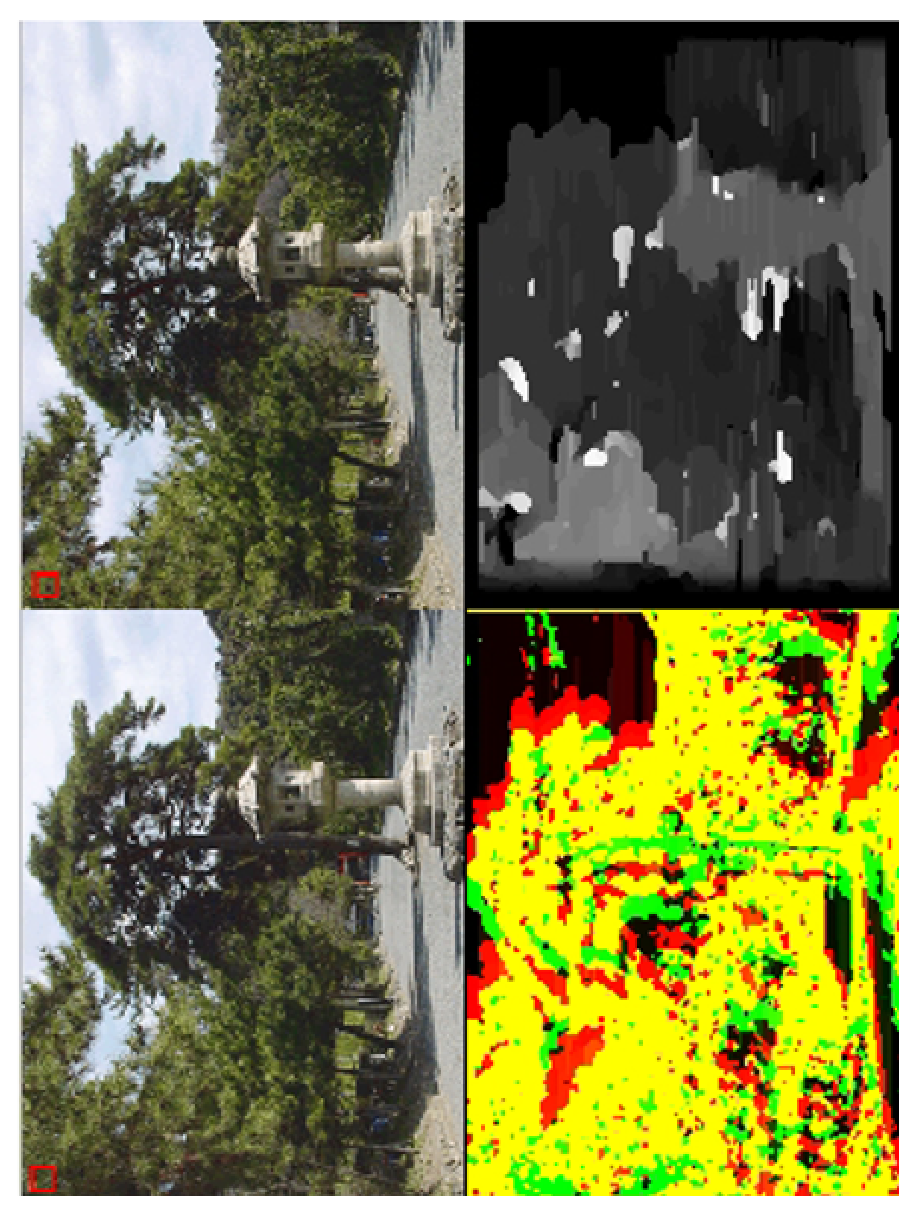
\includegraphics[angle=270,origin=b,width=0.75\textwidth]{stereo.eps}
\caption{Stereo}
\end{figure}

This is a stereo matching with a search size of 12x16. Update SAD for 8 rows by one burst operation. This is not a stencil calculation therefore Mapdist = 0.

\begin{screen}
\tiny
\begin{verbatim}
void wdifline(Uint *l, Uint *r, struct SAD2 *d, int k)
#if !defined(EMAX5) && !defined(EMAX6)
  for (top=DWIN; top<HT-DWIN; top++) { /* scan-lines */
    for (cofs=DWIN+k/2; cofs<WD-DWIN-k/2; cofs++) /* one scan-line */
      d->SAD2[top][cofs] = 0;
  }

  for (top=DWIN; top<HT-DWIN; top++) { /* scan-lines */
    Uint *lp = l + top*WD+k; /* L */
    Uint *rp = r + top*WD; /* R */
    for (pofs1=-DWIN; pofs1<DWIN; pofs1++) {
      Uint *dp = &d->SAD2[top+pofs1][DWIN+k/2];
      for (cofs=0; cofs<WD-DWIN*2; cofs++) { /* one scan-line */
        int x, retval = 0;
        for (x=0; x<DWIN*2; x++)
          retval += df((*(lp+cofs+x))&MASK, (*(rp+cofs+x))&MASK);
        *(dp+cofs) += retval;
      }
    }
  }
#endif
\end{verbatim}
\end{screen}

\begin{screen}
\tiny
\begin{verbatim}
  for (top=0; top<RRANGE; top++) { /* will be parallelized by multi-chip (M/#chip) */
    for (CHIP=0; CHIP<NCHIP; CHIP++) { /* will be parallelized by multi-chip (M/#chip) */
      int idx = CHIP*RRANGE+DWIN+top;
      for (cofs=DWIN+k/2; cofs<WD-DWIN-k/2; cofs++) /* one scan-line */
        d->SAD2[idx][cofs] = 0;
    }
  }

  for (top=0; top<RRANGE; top++) { /* will be parallelized by multi-chip (M/#chip) */
    for (CHIP=0; CHIP<NCHIP; CHIP++) { /* will be parallelized by multi-chip (M/#chip) */
      int  idx = CHIP*RRANGE+DWIN+top;
      Uint *lp = l + idx*WD+k; /* L */
      Uint *rp = r + idx*WD; /* R */
      for (pofs1=-DWIN; pofs1<DWIN; pofs1++) {
        Uint *dp = &d->SAD2[idx+pofs1][DWIN+k/2];
        for (cofs=0; cofs<WD-DWIN*2; cofs++) { /* one scan-line */
          int x, retval = 0;
          for (x=0; x<DWIN*2; x++)
            retval += df((*(lp+cofs+x))&MASK, (*(rp+cofs+x))&MASK);
          *(dp+cofs) += retval;
        }
      }
    }
  }
\end{verbatim}
\end{screen}

\begin{screen}
\tiny
\begin{verbatim}
  Ull  LOOP1, LOOP0;  Ull  INIT1, INIT0;
  Ull  AR[64][4];                     /* output of EX     in each unit */
  Ull  BR[64][4][4];                  /* output registers in each unit */
  Ull  r0, r1, r2, r3, r4, r5, r6, r7, r8, r9, r10, r11, r12, r13, r14, r15;
  Ull  r16, r17, r18, r19, r20, r21, r22, r23, r24, r25, r26, r27, r28, r29, r30, r31;
  Ull  cc0, cc1, cc2, cc3, ex0, ex1;
  for (top=0; top<RRANGE; top++) { /* will be parallelized by multi-chip (M/#chip) */
    for (CHIP=0; CHIP<NCHIP; CHIP++) { /* will be parallelized by multi-chip (M/#chip) */
      int idx = CHIP*RRANGE+DWIN+top;
      for (cofs=DWIN+k/2; cofs<WD-DWIN-k/2; cofs++) /* one scan-line */
        d->SAD2[idx][cofs] = 0;
  } }
  for (top=0; top<RRANGE; top++) { /* scan-lines */
    Uint *lp[NCHIP],  *rp[NCHIP];
    Uint *dp0[NCHIP], *dp1[NCHIP], *dp2[NCHIP], *dp3[NCHIP], *dp4[NCHIP], *dp5[NCHIP], *dp6[NCHIP], *dp7[NCHIP];
    Uint *dp8[NCHIP], *dp9[NCHIP], *dpa[NCHIP], *dpb[NCHIP], *dpc[NCHIP], *dpd[NCHIP], *dpe[NCHIP], *dpf[NCHIP];
    for (CHIP=0; CHIP<NCHIP; CHIP++) { /* will be parallelized by multi-chip (M/#chip) */
      int idx = CHIP*RRANGE+DWIN+top;
      lp[CHIP] = l+idx*WD+k; rp[CHIP] = r+idx*WD;
      dp0[CHIP] = &d->SAD2[idx-8][DWIN+k/2];
      dp1[CHIP] = &d->SAD2[idx-7][DWIN+k/2];
      dp2[CHIP] = &d->SAD2[idx-6][DWIN+k/2];
        :
      dpf[CHIP] = &d->SAD2[idx+7][DWIN+k/2];
    }
//EMAX5A begin wdifline mapdist=0
 /*2*/for (CHIP=0; CHIP<NCHIP; CHIP++) { /* output channels are parallelized by multi-chip (OC/#chip) */
   /*1*/for (INIT0=1,LOOP0=WD,cofs=0-4; LOOP0--; INIT0=0) {       /* stage#0 *//* mapped to FOR() on BR[63][0][0] */
 /*@0,1*/ exe(OP_ADD,      &cofs,        cofs,        EXP_H3210, 4LL,  EXP_H3210, 0LL, EXP_H3210, OP_AND, 0x00000000ffffffffLL, OP_NOP, 0LL);
          /*map0*/
 /*@1,0*/ exe(OP_ADD,      &rofs1,       lp[CHIP],   EXP_H3210, cofs, EXP_H3210,    0, EXP_H3210, OP_NOP,  0LL,  OP_NOP,  0LL);
 /*@1,1*/ exe(OP_ADD,      &rofs2,       rp[CHIP],   EXP_H3210, cofs, EXP_H3210,    0, EXP_H3210, OP_NOP,  0LL,  OP_NOP,  0LL);
 /*@2,0*/ mop(OP_LDWR, 1,  &r2,          rofs1,   0,  MSK_D0,    lp[CHIP],       WD, 0, 0, (Ull)NULL,    WD);
 /*@2,0*/ mop(OP_LDWR, 1,  &r3,          rofs1,   4,  MSK_D0,    lp[CHIP],       WD, 0, 0, (Ull)NULL,    WD);
 /*@2,1*/ mop(OP_LDWR, 1,  &r4,          rofs1,   8,  MSK_D0,    lp[CHIP],       WD, 0, 0, (Ull)NULL,    WD);
 /*@2,1*/ mop(OP_LDWR, 1,  &r5,          rofs1,   12, MSK_D0,    lp[CHIP],       WD, 0, 0, (Ull)NULL,    WD);
 /*@2,2*/ mop(OP_LDWR, 1,  &r6,          rofs2,   0,  MSK_D0,    rp[CHIP],       WD, 0, 0, (Ull)NULL,    WD);
 /*@2,2*/ mop(OP_LDWR, 1,  &r7,          rofs2,   4,  MSK_D0,    rp[CHIP],       WD, 0, 0, (Ull)NULL,    WD);
 /*@2,3*/ mop(OP_LDWR, 1,  &r8,          rofs2,   8,  MSK_D0,    rp[CHIP],       WD, 0, 0, (Ull)NULL,    WD);
 /*@2,3*/ mop(OP_LDWR, 1,  &r9,          rofs2,   12, MSK_D0,    rp[CHIP],       WD, 0, 0, (Ull)NULL,    WD);
 /*@3,0*/ exe(OP_MSAD,     &r22,         r2,          EXP_H3210, r6,   EXP_H3210,    0, EXP_H3210, OP_NOP,  0LL,  OP_NOP,  0LL);
 /*@3,0*/ mop(OP_LDWR, 1,  &r12,         rofs1,   16, MSK_D0,    lp[CHIP],       WD, 0, 0, (Ull)NULL,    WD);
 /*@3,0*/ mop(OP_LDWR, 1,  &r13,         rofs1,   20, MSK_D0,    lp[CHIP],       WD, 0, 0, (Ull)NULL,    WD);
 /*@3,1*/ exe(OP_MSAD,     &r23,         r3,          EXP_H3210, r7,   EXP_H3210,    0, EXP_H3210, OP_NOP,  0LL,  OP_NOP,  0LL);
 /*@3,1*/ mop(OP_LDWR, 1,  &r14,         rofs1,   24, MSK_D0,    lp[CHIP],       WD, 0, 0, (Ull)NULL,    WD);
 /*@3,1*/ mop(OP_LDWR, 1,  &r15,         rofs1,   28, MSK_D0,    lp[CHIP],       WD, 0, 0, (Ull)NULL,    WD);
 /*@3,2*/ exe(OP_MSAD,     &r24,         r4,          EXP_H3210, r8,   EXP_H3210,    0, EXP_H3210, OP_NOP,  0LL,  OP_NOP,  0LL);
 /*@3,2*/ mop(OP_LDWR, 1,  &r16,         rofs2,   16, MSK_D0,    rp[CHIP],       WD, 0, 0, (Ull)NULL,    WD);
 /*@3,2*/ mop(OP_LDWR, 1,  &r17,         rofs2,   20, MSK_D0,    rp[CHIP],       WD, 0, 0, (Ull)NULL,    WD);
 /*@3,3*/ exe(OP_MSAD,     &r25,         r5,          EXP_H3210, r9,   EXP_H3210,    0, EXP_H3210, OP_NOP,  0LL,  OP_NOP,  0LL);
 /*@3,3*/ mop(OP_LDWR, 1,  &r18,         rofs2,   24, MSK_D0,    rp[CHIP],       WD, 0, 0, (Ull)NULL,    WD);
 /*@3,3*/ mop(OP_LDWR, 1,  &r19,         rofs2,   28, MSK_D0,    rp[CHIP],       WD, 0, 0, (Ull)NULL,    WD);
 /*@4,0*/ exe(OP_MSSAD,    &r12,         r22,         EXP_H3210, r12,  EXP_H3210,  r16, EXP_H3210, OP_NOP,  0LL,  OP_NOP,  0LL);
 /*@4,0*/ mop(OP_LDWR, 1,  &r2,          rofs1,   32, MSK_D0,    lp[CHIP],       WD, 0, 0, (Ull)NULL,    WD);
 /*@4,0*/ mop(OP_LDWR, 1,  &r3,          rofs1,   36, MSK_D0,    lp[CHIP],       WD, 0, 0, (Ull)NULL,    WD);
 /*@4,1*/ exe(OP_MSSAD,    &r13,         r23,         EXP_H3210, r13,  EXP_H3210,  r17, EXP_H3210, OP_NOP,  0LL,  OP_NOP,  0LL);
 /*@4,1*/ mop(OP_LDWR, 1,  &r4,          rofs1,   40, MSK_D0,    lp[CHIP],       WD, 0, 0, (Ull)NULL,    WD);
 /*@4,1*/ mop(OP_LDWR, 1,  &r5,          rofs1,   44, MSK_D0,    lp[CHIP],       WD, 0, 0, (Ull)NULL,    WD);
 /*@4,2*/ exe(OP_MSSAD,    &r14,         r24,         EXP_H3210, r14,  EXP_H3210,  r18, EXP_H3210, OP_NOP,  0LL,  OP_NOP,  0LL);
 /*@4,2*/ mop(OP_LDWR, 1,  &r6,          rofs2,   32, MSK_D0,    rp[CHIP],       WD, 0, 0, (Ull)NULL,    WD);
 /*@4,2*/ mop(OP_LDWR, 1,  &r7,          rofs2,   36, MSK_D0,    rp[CHIP],       WD, 0, 0, (Ull)NULL,    WD);
 /*@4,3*/ exe(OP_MSSAD,    &r15,         r25,         EXP_H3210, r15,  EXP_H3210,  r19, EXP_H3210, OP_NOP,  0LL,  OP_NOP,  0LL);
 /*@4,3*/ mop(OP_LDWR, 1,  &r8,          rofs2,   40, MSK_D0,    rp[CHIP],       WD, 0, 0, (Ull)NULL,    WD);
 /*@4,3*/ mop(OP_LDWR, 1,  &r9,          rofs2,   44, MSK_D0,    rp[CHIP],       WD, 0, 0, (Ull)NULL,    WD);
 /*@5,0*/ exe(OP_MSSAD,    &r22,         r12,         EXP_H3210, r2,   EXP_H3210,  r6, EXP_H3210, OP_NOP,  0LL,  OP_NOP,  0LL);
 /*@5,1*/ exe(OP_MSSAD,    &r23,         r13,         EXP_H3210, r3,   EXP_H3210,  r7, EXP_H3210, OP_NOP,  0LL,  OP_NOP,  0LL);
 /*@5,2*/ exe(OP_MSSAD,    &r24,         r14,         EXP_H3210, r4,   EXP_H3210,  r8, EXP_H3210, OP_NOP,  0LL,  OP_NOP,  0LL);
 /*@5,3*/ exe(OP_MSSAD,    &r25,         r15,         EXP_H3210, r5,   EXP_H3210,  r9, EXP_H3210, OP_NOP,  0LL,  OP_NOP,  0LL);
 /*@6,0*/ exe(OP_MAUH3,    &r31,         r22,         EXP_H3210, r23,  EXP_H3210, r24, EXP_H3210, OP_NOP,  0LL,  OP_NOP,  0LL);
 /*@7,0*/ exe(OP_MAUH3,    &r1,          r31,         EXP_H3210, r25,  EXP_H3210,   0, EXP_H3210, OP_SUMHL,0LL,  OP_NOP,  0LL);
 /*@8,0*/ mop(OP_LDWR, 1,  &BR[8][0][1], dp0[CHIP], cofs, MSK_D0, (Ull)dp0[CHIP], WD, 0, 1, (Ull)NULL,    WD);
 /*@8,0*/ exe(OP_ADD,      &AR[8][0],    BR[8][0][1], EXP_H3210, r1,   EXP_H3210,    0, EXP_H3210, OP_NOP,  0LL,  OP_NOP,  0LL);
 /*@8,0*/ mop(OP_STWR, 3,  &AR[8][0],    cofs, dp0[CHIP], MSK_D0, (Ull)dp0[CHIP], WD, 0, 1, (Ull)NULL,    WD);
          /*map1*/
 /*@9,0*/ mop(OP_LDWR, 1,  &BR[9][0][1], dp1[CHIP], cofs, MSK_D0, (Ull)dp1[CHIP], WD, 0, 1, (Ull)NULL,    WD);
 /*@9,0*/ exe(OP_ADD,      &AR[9][0],    BR[9][0][1], EXP_H3210, r1,   EXP_H3210,    0, EXP_H3210, OP_NOP,  0LL,  OP_NOP,  0LL);
 /*@9,0*/ mop(OP_STWR, 3,  &AR[9][0],    cofs, dp1[CHIP], MSK_D0, (Ull)dp1[CHIP], WD, 0, 1, (Ull)NULL,    WD);
          /*map2*/
 /*@10,0*/mop(OP_LDWR, 1,  &BR[10][0][1],dp2[CHIP], cofs, MSK_D0, (Ull)dp2[CHIP], WD, 0, 1, (Ull)NULL,    WD);
 /*@10,0*/exe(OP_ADD,      &AR[10][0],   BR[10][0][1], EXP_H3210,r1,   EXP_H3210,    0, EXP_H3210, OP_NOP,  0LL,  OP_NOP,  0LL);
 /*@10,0*/mop(OP_STWR, 3,  &AR[10][0],   cofs, dp2[CHIP], MSK_D0, (Ull)dp2[CHIP], WD, 0, 1, (Ull)NULL,    WD);
          :
          /*map9*/
 /*@17,0*/mop(OP_LDWR, 1,  &BR[17][0][1],dp9[CHIP], cofs, MSK_D0, (Ull)dp9[CHIP], WD, 0, 1, (Ull)NULL,    WD);
 /*@17,0*/exe(OP_ADD,      &AR[17][0],   BR[17][0][1], EXP_H3210,r1,   EXP_H3210,    0, EXP_H3210, OP_NOP,  0LL,  OP_NOP,  0LL);
 /*@17,0*/mop(OP_STWR, 3,  &AR[17][0],   cofs, dp9[CHIP], MSK_D0, (Ull)dp9[CHIP], WD, 0, 1, (Ull)NULL,    WD);
          /*map10*/
 /*@18,0*/mop(OP_LDWR, 1,  &BR[18][0][1],dpa[CHIP], cofs, MSK_D0, (Ull)dpa[CHIP], WD, 0, 1, (Ull)NULL,    WD);
 /*@18,0*/exe(OP_ADD,      &AR[18][0],   BR[18][0][1], EXP_H3210,r1,   EXP_H3210,    0, EXP_H3210, OP_NOP,  0LL,  OP_NOP,  0LL);
 /*@18,0*/mop(OP_STWR, 3,  &AR[18][0],   cofs, dpa[CHIP], MSK_D0, (Ull)dpa[CHIP], WD, 0, 1, (Ull)NULL,    WD);
          /*map11*/
 /*@19,0*/mop(OP_LDWR, 1,  &BR[19][0][1],dpb[CHIP], cofs, MSK_D0, (Ull)dpb[CHIP], WD, 0, 1, (Ull)NULL,    WD);
 /*@19,0*/exe(OP_ADD,      &AR[19][0],   BR[19][0][1], EXP_H3210,r1,   EXP_H3210,    0, EXP_H3210, OP_NOP,  0LL,  OP_NOP,  0LL);
 /*@19,0*/mop(OP_STWR, 3,  &AR[19][0],   cofs, dpb[CHIP], MSK_D0, (Ull)dpb[CHIP], WD, 0, 1, (Ull)NULL,    WD);
          /*map12*/
 /*@20,0*/mop(OP_LDWR, 1,  &BR[20][0][1],dpc[CHIP], cofs, MSK_D0, (Ull)dpc[CHIP], WD, 0, 1, (Ull)NULL,    WD);
 /*@20,0*/exe(OP_ADD,      &AR[20][0],   BR[20][0][1], EXP_H3210,r1,   EXP_H3210,    0, EXP_H3210, OP_NOP,  0LL,  OP_NOP,  0LL);
 /*@20,0*/mop(OP_STWR, 3,  &AR[20][0],   cofs, dpc[CHIP], MSK_D0, (Ull)dpc[CHIP], WD, 0, 1, (Ull)NULL,    WD);
          /*map13*/
 /*@21,0*/mop(OP_LDWR, 1,  &BR[21][0][1],dpd[CHIP], cofs, MSK_D0, (Ull)dpd[CHIP], WD, 0, 1, (Ull)NULL,    WD);
 /*@21,0*/exe(OP_ADD,      &AR[21][0],   BR[21][0][1], EXP_H3210,r1,   EXP_H3210,    0, EXP_H3210, OP_NOP,  0LL,  OP_NOP,  0LL);
 /*@21,0*/mop(OP_STWR, 3,  &AR[21][0],   cofs, dpd[CHIP], MSK_D0, (Ull)dpd[CHIP], WD, 0, 1, (Ull)NULL,    WD);
          /*map14*/
 /*@22,0*/mop(OP_LDWR, 1,  &BR[22][0][1],dpe[CHIP], cofs, MSK_D0, (Ull)dpe[CHIP], WD, 0, 1, (Ull)NULL,    WD);
 /*@22,0*/exe(OP_ADD,      &AR[22][0],   BR[22][0][1], EXP_H3210,r1,   EXP_H3210,    0, EXP_H3210, OP_NOP,  0LL,  OP_NOP,  0LL);
 /*@22,0*/mop(OP_STWR, 3,  &AR[22][0],   cofs, dpe[CHIP], MSK_D0, (Ull)dpe[CHIP], WD, 0, 1, (Ull)NULL,    WD);
          /*map15*/
 /*@23,0*/mop(OP_LDWR, 1,  &BR[23][0][1],dpf[CHIP], cofs, MSK_D0, (Ull)dpf[CHIP], WD, 0, 1, (Ull)NULL,    WD);
 /*@23,0*/exe(OP_ADD,      &AR[23][0],   BR[23][0][1], EXP_H3210,r1,   EXP_H3210,    0, EXP_H3210, OP_NOP,  0LL,  OP_NOP,  0LL);
 /*@23,0*/mop(OP_STWR, 3,  &AR[23][0],   cofs, dpf[CHIP], MSK_D0, (Ull)dpf[CHIP], WD, 0, 1, (Ull)NULL,    WD);
      } }
//EMAX5A end
  }
//EMAX5A drain_dirty_lmm
\end{verbatim}
\end{screen}

\begin{figure}[htbp]
\center
\epsfile{file=filter+rmm-wdifline-emax6.eps,width=1.00\textwidth}
\caption{Stereo with stencil}
\end{figure}

\clearpage

\section{3D-floating-point}

\shabox{
\leftline{cent\% make -f Makefile-csim.emax6+dma all clean}
\leftline{cent\% ../../src/csim/csim -x stencil-csim.emax6+dma}
}

\shabox{
\leftline{zynq\% make -f Makefile-zynq.emax6+dma all clean}
\leftline{zynq\% ./stencil-zynq.emax6+dma}
}

\subsection{Grapes with stencil}

\begin{figure}[htbp]
\center
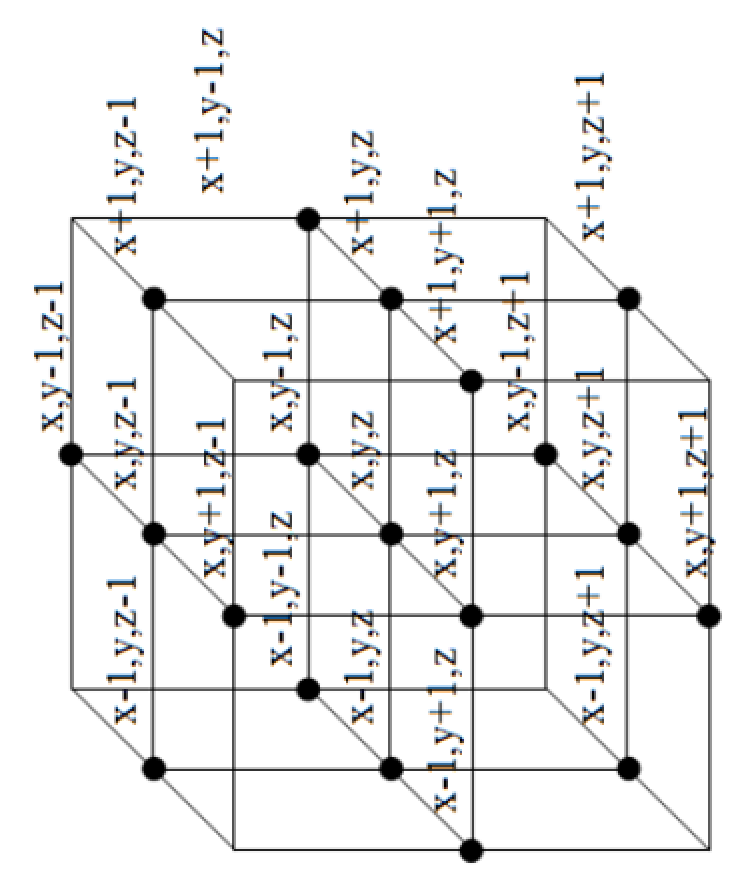
\includegraphics[angle=270,origin=b,width=0.30\textwidth]{grapes.eps}
\caption{Grapes}
\end{figure}

This is a 19-point floating-point stencil calculation. Although array A does not have a stencil property, 12 rows are calculated by one burst operation to reduce the number of initial times (RMGRP = 12). Since array B is reusable, mapdist = 1.

\begin{screen}
\tiny
\begin{verbatim}
grapes( float *c, float *a, float *b )
     /*C3D[DP][HT][WD]*/
     /*GrA[XC][DP][HT][WD]*/
     /*B3D[DP][HT][WD]*/
#define NCHIP     1
#define RMGRP     12
#define OMAP      1
#define PAD       1
#define RRANGE   ((HT-PAD*2)/NCHIP/OMAP)
  Ull  CHIP;
  Ull  LOOP1, LOOP0;
  Ull  INIT1, INIT0;
  Ull  AR[64][4];                     /* output of EX     in each unit */
  Ull  BR[64][4][4];                  /* output registers in each unit */
  Ull  r0, r1, r2, r3, r4, r5, r6, r7, r8, r9, r10, r11, r12, r13, r14, r15;
  Ull  r16, r17, r18, r19, r20, r21, r22, r23, r24, r25, r26, r27, r28, r29, r30, r31;
  Ull  cc0, cc1, cc2, cc3, ex0, ex1;
  int  x, y, z;
  int  row, col, n;
  Ull  roofs, coofs, aofs, bofs, cofs;

#if !defined(EMAX5) && !defined(EMAX6)
  for (z=PAD; z<DP-PAD; z++) {
    for (y=PAD; y<HT-PAD; y++) {
      for (x=PAD; x<WD-PAD; x++) {
        *(c+z*WDHT+y*WD+x) = *(b+(z-1)*WDHT+(y-1)*WD+x  ) * *(a+(MID-6)*WDHTDP+(z-1)*WDHT+(y-1)*WD+x  ) /* braw00 */ /* araw00 */
                           + *(b+(z-1)*WDHT+(y  )*WD+x-1) * *(a+(MID-5)*WDHTDP+(z-1)*WDHT+(y  )*WD+x-1) /* braw01 */ /* araw01 */
                           + *(b+(z-1)*WDHT+(y  )*WD+x  ) * *(a+(MID-4)*WDHTDP+(z-1)*WDHT+(y  )*WD+x  ) /* braw01 */ /* araw02 */
                           + *(b+(z-1)*WDHT+(y  )*WD+x+1) * *(a+(MID-5)*WDHTDP+(z-1)*WDHT+(y  )*WD+x+1) /* braw01 */ /* araw01 */
                           + *(b+(z-1)*WDHT+(y+1)*WD+x  ) * *(a+(MID-3)*WDHTDP+(z-1)*WDHT+(y+1)*WD+x  ) /* braw02 */ /* araw03 */
                           + *(b+(z  )*WDHT+(y-1)*WD+x-1) * *(a+(MID-2)*WDHTDP+(z  )*WDHT+(y-1)*WD+x-1) /* braw03 */ /* araw04 */
                           + *(b+(z  )*WDHT+(y-1)*WD+x  ) * *(a+(MID-1)*WDHTDP+(z  )*WDHT+(y-1)*WD+x  ) /* braw03 */ /* araw05 */
                           + *(b+(z  )*WDHT+(y-1)*WD+x+1) * *(a+(MID-2)*WDHTDP+(z  )*WDHT+(y-1)*WD+x+1) /* braw03 */ /* araw04 */
                           + *(b+(z  )*WDHT+(y  )*WD+x-1) * *(a+(MID  )*WDHTDP+(z  )*WDHT+(y  )*WD+x-1) /* braw04 */ /* araw06 */
                           + *(b+(z  )*WDHT+(y  )*WD+x  )                                               /* braw04 */
                           + *(b+(z  )*WDHT+(y  )*WD+x+1) * *(a+(MID  )*WDHTDP+(z  )*WDHT+(y  )*WD+x+1) /* braw04 */ /* araw06 */
                           + *(b+(z  )*WDHT+(y+1)*WD+x-1) * *(a+(MID+2)*WDHTDP+(z  )*WDHT+(y+1)*WD+x-1) /* braw05 */ /* araw08 */
                           + *(b+(z  )*WDHT+(y+1)*WD+x  ) * *(a+(MID+1)*WDHTDP+(z  )*WDHT+(y+1)*WD+x  ) /* braw05 */ /* araw07 */
                           + *(b+(z  )*WDHT+(y+1)*WD+x+1) * *(a+(MID+2)*WDHTDP+(z  )*WDHT+(y+1)*WD+x+1) /* braw05 */ /* araw08 */
                           + *(b+(z+1)*WDHT+(y-1)*WD+x  ) * *(a+(MID+3)*WDHTDP+(z+1)*WDHT+(y-1)*WD+x  ) /* braw06 */ /* araw09 */
                           + *(b+(z+1)*WDHT+(y  )*WD+x-1) * *(a+(MID+5)*WDHTDP+(z+1)*WDHT+(y  )*WD+x-1) /* braw07 */ /* araw0b */
                           + *(b+(z+1)*WDHT+(y  )*WD+x  ) * *(a+(MID+4)*WDHTDP+(z+1)*WDHT+(y  )*WD+x  ) /* braw07 */ /* araw0a */
                           + *(b+(z+1)*WDHT+(y  )*WD+x+1) * *(a+(MID+5)*WDHTDP+(z+1)*WDHT+(y  )*WD+x+1) /* braw07 */ /* araw0b */
                           + *(b+(z+1)*WDHT+(y+1)*WD+x  ) * *(a+(MID+6)*WDHTDP+(z+1)*WDHT+(y+1)*WD+x  );/* braw08 */ /* araw0c */
      }
    }
  }
#endif
\end{verbatim}
\end{screen}

\begin{screen}
\tiny
\begin{verbatim}
  for (z=PAD; z<DP-PAD; z++) {
    for (y=0; y<RRANGE; y+=RMGRP) {
      Ull  atop[NCHIP], btop[NCHIP], ctop[NCHIP];
      Ull  arow00[NCHIP], arow01[NCHIP], arow02[NCHIP], arow03[NCHIP], arow04[NCHIP], arow05[NCHIP], arow06[NCHIP], arow07[NCHIP], arow08[NCHIP],
           arow09[NCHIP], arow0a[NCHIP], arow0b[NCHIP], arow0c[NCHIP];
      Ull  brow00[NCHIP], brow01[NCHIP], brow02[NCHIP], brow03[NCHIP], brow04[NCHIP], brow05[NCHIP], brow06[NCHIP], brow07[NCHIP], brow08[NCHIP];
      Ull  crow0[NCHIP];
      for (CHIP=0; CHIP<NCHIP; CHIP++) { /* output channels are parallelized by multi-chip (OC/#chip) */
        atop[CHIP]   = a               +(z  )*WDHT+(CHIP*RRANGE*OMAP+RRANGE*0+PAD+y  )*WD;
        btop[CHIP]   = b               +(z  )*WDHT+(CHIP*RRANGE*OMAP+RRANGE*0+PAD+y  )*WD;
        ctop[CHIP]   = c               +(z  )*WDHT+(CHIP*RRANGE*OMAP+RRANGE*0+PAD+y  )*WD;
        arow00[CHIP] = a+(MID-6)*WDHTDP+(z-1)*WDHT+(CHIP*RRANGE*OMAP+RRANGE*0+PAD+y-1)*WD;
        arow01[CHIP] = a+(MID-5)*WDHTDP+(z-1)*WDHT+(CHIP*RRANGE*OMAP+RRANGE*0+PAD+y  )*WD;
        arow02[CHIP] = a+(MID-4)*WDHTDP+(z-1)*WDHT+(CHIP*RRANGE*OMAP+RRANGE*0+PAD+y  )*WD;
        arow03[CHIP] = a+(MID-3)*WDHTDP+(z-1)*WDHT+(CHIP*RRANGE*OMAP+RRANGE*0+PAD+y+1)*WD;
        arow04[CHIP] = a+(MID-2)*WDHTDP+(z  )*WDHT+(CHIP*RRANGE*OMAP+RRANGE*0+PAD+y-1)*WD;
        arow05[CHIP] = a+(MID-1)*WDHTDP+(z  )*WDHT+(CHIP*RRANGE*OMAP+RRANGE*0+PAD+y-1)*WD;
        arow06[CHIP] = a+(MID  )*WDHTDP+(z  )*WDHT+(CHIP*RRANGE*OMAP+RRANGE*0+PAD+y  )*WD;
        arow07[CHIP] = a+(MID+1)*WDHTDP+(z  )*WDHT+(CHIP*RRANGE*OMAP+RRANGE*0+PAD+y+1)*WD;
        arow08[CHIP] = a+(MID+2)*WDHTDP+(z  )*WDHT+(CHIP*RRANGE*OMAP+RRANGE*0+PAD+y+1)*WD;
        arow09[CHIP] = a+(MID+3)*WDHTDP+(z+1)*WDHT+(CHIP*RRANGE*OMAP+RRANGE*0+PAD+y-1)*WD;
        arow0a[CHIP] = a+(MID+4)*WDHTDP+(z+1)*WDHT+(CHIP*RRANGE*OMAP+RRANGE*0+PAD+y  )*WD;
        arow0b[CHIP] = a+(MID+5)*WDHTDP+(z+1)*WDHT+(CHIP*RRANGE*OMAP+RRANGE*0+PAD+y  )*WD;
        arow0c[CHIP] = a+(MID+6)*WDHTDP+(z+1)*WDHT+(CHIP*RRANGE*OMAP+RRANGE*0+PAD+y+1)*WD;
        brow00[CHIP] = b               +(z-1)*WDHT+(CHIP*RRANGE*OMAP+RRANGE*0+PAD+y-1)*WD;
        brow01[CHIP] = b               +(z-1)*WDHT+(CHIP*RRANGE*OMAP+RRANGE*0+PAD+y  )*WD;
        brow02[CHIP] = b               +(z-1)*WDHT+(CHIP*RRANGE*OMAP+RRANGE*0+PAD+y+1)*WD;
        brow03[CHIP] = b               +(z  )*WDHT+(CHIP*RRANGE*OMAP+RRANGE*0+PAD+y-1)*WD;
        brow04[CHIP] = b               +(z  )*WDHT+(CHIP*RRANGE*OMAP+RRANGE*0+PAD+y  )*WD;
        brow05[CHIP] = b               +(z  )*WDHT+(CHIP*RRANGE*OMAP+RRANGE*0+PAD+y+1)*WD;
        brow06[CHIP] = b               +(z+1)*WDHT+(CHIP*RRANGE*OMAP+RRANGE*0+PAD+y-1)*WD;
        brow07[CHIP] = b               +(z+1)*WDHT+(CHIP*RRANGE*OMAP+RRANGE*0+PAD+y  )*WD;
        brow08[CHIP] = b               +(z+1)*WDHT+(CHIP*RRANGE*OMAP+RRANGE*0+PAD+y+1)*WD;
        crow0[CHIP]  = c               +(z  )*WDHT+(CHIP*RRANGE*OMAP+RRANGE*0+PAD+y  )*WD;
      }
//EMAX5A begin grapes mapdist=1
      for (CHIP=0; CHIP<NCHIP; CHIP++) { /* output channels are parallelized by multi-chip (OC/#chip) */
   /*2*/for (INIT1=1,LOOP1=RMGRP,roofs=0-WD*4; LOOP1--; INIT1=0) {      /* stage#0 *//* mapped to FOR() on BR[63][1][0] */
     /*1*/for (INIT0=1,LOOP0=WD-PAD*2,coofs=(PAD-1)*4; LOOP0--; INIT0=0) {          /* stage#0 *//* mapped to FOR() on BR[63][0][0] */
            exe(OP_ADD,  &coofs, INIT0?coofs:coofs, EXP_H3210, 4, EXP_H3210, 0LL, EXP_H3210, OP_AND, 0x00000000ffffffffLL, OP_NOP, 0LL); /* stage#0 */
            exe(OP_ADD,  &roofs, roofs,  EXP_H3210, INIT0?WD*4:0, EXP_H3210, 0LL, EXP_H3210, OP_AND, 0x00000000ffffffffLL, OP_NOP, 0LL); /* stage#0 */
            exe(OP_ADD3, &aofs,  atop[CHIP], EXP_H3210, roofs, EXP_H3210,  coofs, EXP_H3210, OP_AND, 0x000000ffffffffffLL, OP_NOP, 0LL); /* stage#1 */
            exe(OP_ADD3, &bofs,  btop[CHIP], EXP_H3210, roofs, EXP_H3210,  coofs, EXP_H3210, OP_AND, 0x000000ffffffffffLL, OP_NOP, 0LL); /* stage#1 */
            exe(OP_ADD3, &cofs,  ctop[CHIP], EXP_H3210, roofs, EXP_H3210,  coofs, EXP_H3210, OP_AND, 0x000000ffffffffffLL, OP_NOP, 0LL); /* stage#1 */
            /*map0*/
            mop(OP_LDWR, 1, &BR[2][0][1], bofs, (0               -WDHT-WD  )*4, MSK_D0, brow00[CHIP], WD*(RMGRP+PAD*2), 0, 0, (Ull)NULL, WD*(RMGRP+PAD*2));/*st#2*/
            mop(OP_LDWR, 1, &BR[2][2][1], aofs, (0+WDHTDP*(MID-6)-WDHT-WD  )*4, MSK_D0, arow00[CHIP], WD*RMGRP, 0, 0, (Ull)NULL, WD*RMGRP);/* stage#2 */
            exe(OP_FML, &r0, BR[2][0][1], EXP_H3210,  BR[2][2][1], EXP_H3210, 0,           EXP_H3210, OP_NOP, 0LL, OP_NOP, 0LL);         /* stage#3 */
            mop(OP_LDWR, 1, &BR[3][0][1], bofs, (0               -WDHT   -1)*4, MSK_D0, brow00[CHIP], WD*(RMGRP+PAD*2), 0, 0, (Ull)NULL, WD*(RMGRP+PAD*2));/*st#3*/
            mop(OP_LDWR, 1, &BR[3][0][0], bofs, (0               -WDHT   +1)*4, MSK_D0, brow00[CHIP], WD*(RMGRP+PAD*2), 0, 0, (Ull)NULL, WD*(RMGRP+PAD*2));/*st#3*/
            mop(OP_LDWR, 1, &BR[3][1][1], bofs, (0               -WDHT     )*4, MSK_D0, brow00[CHIP], WD*(RMGRP+PAD*2), 0, 0, (Ull)NULL, WD*(RMGRP+PAD*2));/*st#3*/
            mop(OP_LDWR, 1, &BR[3][2][1], aofs, (0+WDHTDP*(MID-5)-WDHT   -1)*4, MSK_D0, arow01[CHIP], WD*RMGRP, 0, 0, (Ull)NULL, WD*RMGRP);/* stage#3 */
            mop(OP_LDWR, 1, &BR[3][2][0], aofs, (0+WDHTDP*(MID-5)-WDHT   +1)*4, MSK_D0, arow01[CHIP], WD*RMGRP, 0, 0, (Ull)NULL, WD*RMGRP);/* stage#3 */
            mop(OP_LDWR, 1, &BR[3][3][1], aofs, (0+WDHTDP*(MID-4)-WDHT     )*4, MSK_D0, arow02[CHIP], WD*RMGRP, 0, 0, (Ull)NULL, WD*RMGRP);/* stage#3 */
            exe(OP_FMA, &r1, r0,          EXP_H3210,  BR[3][0][1], EXP_H3210, BR[3][2][1], EXP_H3210, OP_NOP, 0LL, OP_NOP, 0LL);         /* stage#4 */
            exe(OP_FML, &r2, BR[3][0][0], EXP_H3210,  BR[3][2][0], EXP_H3210, 0,           EXP_H3210, OP_NOP, 0LL, OP_NOP, 0LL);         /* stage#4 */
            exe(OP_FML, &r3, BR[3][1][1], EXP_H3210,  BR[3][3][1], EXP_H3210, 0,           EXP_H3210, OP_NOP, 0LL, OP_NOP, 0LL);         /* stage#4 */
            mop(OP_LDWR, 1, &BR[4][0][1], bofs, (0               -WDHT+WD  )*4, MSK_D0, brow00[CHIP], WD*(RMGRP+PAD*2), 0, 0, (Ull)NULL, WD*(RMGRP+PAD*2));/*st#4*/
            mop(OP_LDWR, 1, &BR[4][2][1], aofs, (0+WDHTDP*(MID-3)-WDHT+WD  )*4, MSK_D0, arow03[CHIP], WD*RMGRP, 0, 0, (Ull)NULL, WD*RMGRP);/* stage#4 */
            exe(OP_FMA, &r4, r1,          EXP_H3210,  BR[4][0][1], EXP_H3210, BR[4][2][1], EXP_H3210, OP_NOP, 0LL, OP_NOP, 0LL);         /* stage#5 */
            exe(OP_FAD, &r5, r2,          EXP_H3210,  r3,          EXP_H3210, 0,           EXP_H3210, OP_NOP, 0LL, OP_NOP, 0LL);         /* stage#5 */

            mop(OP_LDWR, 1, &BR[6][0][1], bofs, (0                    -WD-1)*4, MSK_D0, brow03[CHIP], WD*(RMGRP+PAD*2), 0, 0, (Ull)NULL, WD*(RMGRP+PAD*2));/*st#6*/
            mop(OP_LDWR, 1, &BR[6][0][0], bofs, (0                    -WD+1)*4, MSK_D0, brow03[CHIP], WD*(RMGRP+PAD*2), 0, 0, (Ull)NULL, WD*(RMGRP+PAD*2));/*st#6*/
            mop(OP_LDWR, 1, &BR[6][1][1], bofs, (0                    -WD  )*4, MSK_D0, brow03[CHIP], WD*(RMGRP+PAD*2), 0, 0, (Ull)NULL, WD*(RMGRP+PAD*2));/*st#6*/
            mop(OP_LDWR, 1, &BR[6][2][1], aofs, (0+WDHTDP*(MID-2)     -WD-1)*4, MSK_D0, arow04[CHIP], WD*RMGRP, 0, 0, (Ull)NULL, WD*RMGRP);/* stage#6 */
            mop(OP_LDWR, 1, &BR[6][2][0], aofs, (0+WDHTDP*(MID-2)     -WD+1)*4, MSK_D0, arow04[CHIP], WD*RMGRP, 0, 0, (Ull)NULL, WD*RMGRP);/* stage#6 */
            mop(OP_LDWR, 1, &BR[6][3][1], aofs, (0+WDHTDP*(MID-1)     -WD  )*4, MSK_D0, arow05[CHIP], WD*RMGRP, 0, 0, (Ull)NULL, WD*RMGRP);/* stage#6 */
            exe(OP_FMA, &r0, r4,          EXP_H3210,  BR[6][0][1], EXP_H3210, BR[6][2][1], EXP_H3210, OP_NOP, 0LL, OP_NOP, 0LL);           /* stage#7 */
            exe(OP_FMA, &r1, r5,          EXP_H3210,  BR[6][0][0], EXP_H3210, BR[6][2][0], EXP_H3210, OP_NOP, 0LL, OP_NOP, 0LL);           /* stage#7 */
            exe(OP_FML, &r2, BR[6][1][1], EXP_H3210,  BR[6][3][1], EXP_H3210, 0,           EXP_H3210, OP_NOP, 0LL, OP_NOP, 0LL);           /* stage#7 */
            mop(OP_LDWR, 1, &BR[7][0][1], bofs, (0                       -1)*4, MSK_D0, brow03[CHIP], WD*(RMGRP+PAD*2), 0, 0, (Ull)NULL, WD*(RMGRP+PAD*2));/*st#7*/
            mop(OP_LDWR, 1, &BR[7][0][0], bofs, (0                       +1)*4, MSK_D0, brow03[CHIP], WD*(RMGRP+PAD*2), 0, 0, (Ull)NULL, WD*(RMGRP+PAD*2));/*st#7*/
            mop(OP_LDWR, 1, &BR[7][1][1], bofs, (0                         )*4, MSK_D0, brow03[CHIP], WD*(RMGRP+PAD*2), 0, 0, (Ull)NULL, WD*(RMGRP+PAD*2));/*st#7*/
            mop(OP_LDWR, 1, &BR[7][2][1], aofs, (0+WDHTDP*(MID  )        -1)*4, MSK_D0, arow06[CHIP], WD*RMGRP, 0, 0, (Ull)NULL, WD*RMGRP);/* stage#7 */
            mop(OP_LDWR, 1, &BR[7][2][0], aofs, (0+WDHTDP*(MID  )        +1)*4, MSK_D0, arow06[CHIP], WD*RMGRP, 0, 0, (Ull)NULL, WD*RMGRP);/* stage#7 */
            exe(OP_FMA, &r3, r0,          EXP_H3210,  BR[7][0][1], EXP_H3210, BR[7][2][1], EXP_H3210, OP_NOP, 0LL, OP_NOP, 0LL);           /* stage#8 */
            exe(OP_FMA, &r4, r1,          EXP_H3210,  BR[7][0][0], EXP_H3210, BR[7][2][0], EXP_H3210, OP_NOP, 0LL, OP_NOP, 0LL);           /* stage#8 */
            exe(OP_FAD, &r5, r2,          EXP_H3210,  BR[7][1][1], EXP_H3210, 0,           EXP_H3210, OP_NOP, 0LL, OP_NOP, 0LL);           /* stage#8 */
            mop(OP_LDWR, 1, &BR[8][0][1], bofs, (0                    +WD-1)*4, MSK_D0, brow03[CHIP], WD*(RMGRP+PAD*2), 0, 0, (Ull)NULL, WD*(RMGRP+PAD*2));/*st#8*/
            mop(OP_LDWR, 1, &BR[8][0][0], bofs, (0                    +WD+1)*4, MSK_D0, brow03[CHIP], WD*(RMGRP+PAD*2), 0, 0, (Ull)NULL, WD*(RMGRP+PAD*2));/*st#8*/
            mop(OP_LDWR, 1, &BR[8][1][1], bofs, (0                    +WD  )*4, MSK_D0, brow03[CHIP], WD*(RMGRP+PAD*2), 0, 0, (Ull)NULL, WD*(RMGRP+PAD*2));/*st#8*/
            mop(OP_LDWR, 1, &BR[8][2][1], aofs, (0+WDHTDP*(MID+2)     +WD-1)*4, MSK_D0, arow08[CHIP], WD*RMGRP, 0, 0, (Ull)NULL, WD*RMGRP);/* stage#8 */
            mop(OP_LDWR, 1, &BR[8][2][0], aofs, (0+WDHTDP*(MID+2)     +WD+1)*4, MSK_D0, arow08[CHIP], WD*RMGRP, 0, 0, (Ull)NULL, WD*RMGRP);/* stage#8 */
            mop(OP_LDWR, 1, &BR[8][3][1], aofs, (0+WDHTDP*(MID+1)     +WD  )*4, MSK_D0, arow07[CHIP], WD*RMGRP, 0, 0, (Ull)NULL, WD*RMGRP);/* stage#8 */
            exe(OP_FMA, &r6, r3,          EXP_H3210,  BR[8][0][1], EXP_H3210, BR[8][2][1], EXP_H3210, OP_NOP, 0LL, OP_NOP, 0LL);           /* stage#9 */
            exe(OP_FMA, &r7, r4,          EXP_H3210,  BR[8][0][0], EXP_H3210, BR[8][2][0], EXP_H3210, OP_NOP, 0LL, OP_NOP, 0LL);           /* stage#9 */
            exe(OP_FMA, &r8, r5,          EXP_H3210,  BR[8][1][1], EXP_H3210, BR[8][3][1], EXP_H3210, OP_NOP, 0LL, OP_NOP, 0LL);           /* stage#9 */

            mop(OP_LDWR, 1, &BR[10][0][1],bofs, (0               +WDHT-WD  )*4, MSK_D0, brow06[CHIP], WD*(RMGRP+PAD*2), 0, 0, (Ull)NULL, WD*(RMGRP+PAD*2));/*st#10*/
            mop(OP_LDWR, 1, &BR[10][2][1],aofs, (0+WDHTDP*(MID+3)+WDHT-WD  )*4, MSK_D0, arow09[CHIP], WD*RMGRP, 0, 0, (Ull)NULL, WD*RMGRP);/* stage#10*/
            exe(OP_FMA, &r0, r6,          EXP_H3210,  BR[10][0][1],EXP_H3210, BR[10][2][1],EXP_H3210, OP_NOP, 0LL, OP_NOP, 0LL);           /* stage#11*/
            exe(OP_FAD, &r1, r7,          EXP_H3210,  r8,          EXP_H3210, 0,           EXP_H3210, OP_NOP, 0LL, OP_NOP, 0LL);           /* stage#11*/
            mop(OP_LDWR, 1, &BR[11][0][1],bofs, (0               +WDHT   -1)*4, MSK_D0, brow06[CHIP], WD*(RMGRP+PAD*2), 0, 0, (Ull)NULL, WD*(RMGRP+PAD*2));/*st#11*/
            mop(OP_LDWR, 1, &BR[11][0][0],bofs, (0               +WDHT   +1)*4, MSK_D0, brow06[CHIP], WD*(RMGRP+PAD*2), 0, 0, (Ull)NULL, WD*(RMGRP+PAD*2));/*st#11*/
            mop(OP_LDWR, 1, &BR[11][1][1],bofs, (0               +WDHT     )*4, MSK_D0, brow06[CHIP], WD*(RMGRP+PAD*2), 0, 0, (Ull)NULL, WD*(RMGRP+PAD*2));/*st#11*/
            mop(OP_LDWR, 1, &BR[11][2][1],aofs, (0+WDHTDP*(MID+5)+WDHT   -1)*4, MSK_D0, arow0b[CHIP], WD*RMGRP, 0, 0, (Ull)NULL, WD*RMGRP);/* stage#11*/
            mop(OP_LDWR, 1, &BR[11][2][0],aofs, (0+WDHTDP*(MID+5)+WDHT   +1)*4, MSK_D0, arow0b[CHIP], WD*RMGRP, 0, 0, (Ull)NULL, WD*RMGRP);/* stage#11*/
            mop(OP_LDWR, 1, &BR[11][3][1],aofs, (0+WDHTDP*(MID+4)+WDHT     )*4, MSK_D0, arow0a[CHIP], WD*RMGRP, 0, 0, (Ull)NULL, WD*RMGRP);/* stage#11*/
            exe(OP_FMA, &r2, r0,          EXP_H3210,  BR[11][0][1],EXP_H3210, BR[11][2][1],EXP_H3210, OP_NOP, 0LL, OP_NOP, 0LL);           /* stage#12*/
            exe(OP_FMA, &r3, r1,          EXP_H3210,  BR[11][0][0],EXP_H3210, BR[11][2][0],EXP_H3210, OP_NOP, 0LL, OP_NOP, 0LL);           /* stage#12*/
            exe(OP_FML, &r4, BR[11][1][1],EXP_H3210,  BR[11][3][1],EXP_H3210, 0,           EXP_H3210, OP_NOP, 0LL, OP_NOP, 0LL);           /* stage#12*/
            mop(OP_LDWR, 1, &BR[12][0][1],bofs, (0               +WDHT+WD  )*4, MSK_D0, brow06[CHIP], WD*(RMGRP+PAD*2), 0, 0, (Ull)NULL, WD*(RMGRP+PAD*2));/*st#12*/
            mop(OP_LDWR, 1, &BR[12][2][1],aofs, (0+WDHTDP*(MID+6)+WDHT+WD  )*4, MSK_D0, arow0c[CHIP], WD*RMGRP, 0, 0, (Ull)NULL, WD*RMGRP);/* stage#12*/
            exe(OP_FMA, &r5, r2,          EXP_H3210,  BR[12][0][1],EXP_H3210, BR[12][2][1],EXP_H3210, OP_NOP, 0LL, OP_NOP, 0LL);           /* stage#13*/
            exe(OP_FAD, &r6, r3,          EXP_H3210,  r4,          EXP_H3210, 0,           EXP_H3210, OP_NOP, 0LL, OP_NOP, 0LL);           /* stage#13*/
            exe(OP_FAD, &r7, r5,          EXP_H3210,  r6,          EXP_H3210, 0,           EXP_H3210, OP_NOP, 0LL, OP_NOP, 0LL);           /* stage#14*/
            mop(OP_STWR, 3, &r7,          cofs, (0                         )*4, MSK_D0, crow0[CHIP],  WD*RMGRP, 0, 0, (Ull)NULL, WD*RMGRP);/* stage#14*/
          }
        }
      }
//EMAX5A end
    }
//EMAX5A drain_dirty_lmm
  }
\end{verbatim}
\end{screen}

\begin{figure}[htbp]
\center
\epsfile{file=stencil+rmm-grapes-emax6.eps,width=1.00\textwidth}
\caption{Grapes}
\end{figure}

\clearpage

\subsection{Jacobi with stencil}

\begin{figure}[htbp]
\center
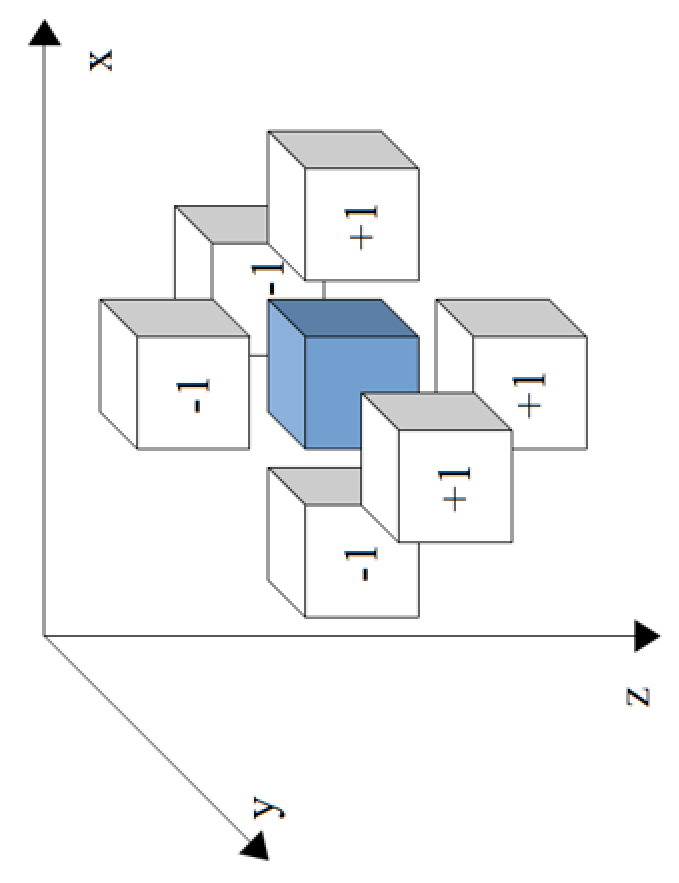
\includegraphics[angle=270,origin=b,width=0.75\textwidth]{jacobi.eps}
\caption{Jacobi}
\end{figure}

Here is a 7-point floating-point stencil calculation. Calculate 24 rows by one burst operation (RMGRP = 24). Although it is a stencil calculation, mapdist = 0 because it calculates 24 lines at a time.

\begin{screen}
\tiny
\begin{verbatim}
jacobi( float *c, float *b )
     /*C3D[DP][HT][WD]*/
     /*B3D[DP][HT][WD]*/
#undef  NCHIP
#undef  RMGRP
#undef  OMAP
#undef  PAD
#undef  RRANGE
#define NCHIP     1
#define RMGRP     24
#define OMAP      1
#define PAD       1
#define RRANGE   ((HT-PAD*2)/NCHIP/OMAP)
  Ull  CHIP;
  Ull  LOOP1, LOOP0;
  Ull  INIT1, INIT0;
  Ull  AR[64][4];                     /* output of EX     in each unit */
  Ull  BR[64][4][4];                  /* output registers in each unit */
  Ull  r0, r1, r2, r3, r4, r5, r6, r7, r8, r9, r10, r11, r12, r13, r14, r15;
  Ull  r16, r17, r18, r19, r20, r21, r22, r23, r24, r25, r26, r27, r28, r29, r30, r31;
  Ull  cc0, cc1, cc2, cc3, ex0, ex1;
  int  x, y, z;
  int  row, col, n;
  Ull  roofs, coofs, aofs, bofs, cofs;
  union {float f; int i;} C1, C2;
  C1.f = 0.2;
  C2.f = 0.3;
  Ull  I1 = C1.i;
  Ull  I2 = C2.i;

#if !defined(EMAX5) && !defined(EMAX6)
  for (z=PAD; z<DP-PAD; z++) {
    for (y=PAD; y<HT-PAD; y++) {
      for (x=PAD; x<WD-PAD; x++) {
        *(c+z*WDHT+y*WD+x) = C2.f *(*(b+(z-1)*WDHT+(y  )*WD+x  )
                                  + *(b+(z  )*WDHT+(y-1)*WD+x  )
                                  + *(b+(z  )*WDHT+(y  )*WD+x-1)
                                  + *(b+(z  )*WDHT+(y  )*WD+x+1)
                                  + *(b+(z  )*WDHT+(y+1)*WD+x  )
                                  + *(b+(z+1)*WDHT+(y  )*WD+x  ))
                           + C1.f * *(b+(z  )*WDHT+(y  )*WD+x  );
      }
    }
  }
#endif
\end{verbatim}
\end{screen}

\begin{screen}
\tiny
\begin{verbatim}
  for (z=PAD; z<DP-PAD; z++) {
    for (y=0; y<RRANGE; y+=RMGRP) {
      Ull  btop[NCHIP], ctop[NCHIP];
      Ull  brow00[NCHIP], brow01[NCHIP], brow02[NCHIP], brow03[NCHIP], brow04[NCHIP];
      Ull  crow0[NCHIP];
      for (CHIP=0; CHIP<NCHIP; CHIP++) { /* output channels are parallelized by multi-chip (OC/#chip) */
        btop[CHIP]   = b               +(z  )*WDHT+(CHIP*RRANGE*OMAP+RRANGE*0+PAD+y  )*WD;
        ctop[CHIP]   = c               +(z  )*WDHT+(CHIP*RRANGE*OMAP+RRANGE*0+PAD+y  )*WD;
        brow00[CHIP] = b               +(z-1)*WDHT+(CHIP*RRANGE*OMAP+RRANGE*0+PAD+y  )*WD;
        brow01[CHIP] = b               +(z+1)*WDHT+(CHIP*RRANGE*OMAP+RRANGE*0+PAD+y  )*WD;
        brow02[CHIP] = b               +(z  )*WDHT+(CHIP*RRANGE*OMAP+RRANGE*0+PAD+y-1)*WD;
        brow03[CHIP] = b               +(z  )*WDHT+(CHIP*RRANGE*OMAP+RRANGE*0+PAD+y  )*WD;/* not used for RMGRP>1 */
        brow04[CHIP] = b               +(z  )*WDHT+(CHIP*RRANGE*OMAP+RRANGE*0+PAD+y+1)*WD;/* not used for RMGRP>1 */
        crow0[CHIP]  = c               +(z  )*WDHT+(CHIP*RRANGE*OMAP+RRANGE*0+PAD+y  )*WD;
      }
//EMAX5A begin jacobi mapdist=0 /* 7 PAD>0�ξ��,PLOAD��LOAD�ΰ褬������ʣ.load���LMM�ˤ�PLOAD������ि��˽��ڤ�ȯ������ */
      for (CHIP=0; CHIP<NCHIP; CHIP++) { /* output channels are parallelized by multi-chip (OC/#chip) */
   /*2*/for (INIT1=1,LOOP1=RMGRP,roofs=0-WD*4; LOOP1--; INIT1=0) {      /* stage#0 *//* mapped to FOR() on BR[63][1][0] */
     /*1*/for (INIT0=1,LOOP0=WD-PAD*2,coofs=(PAD-1)*4; LOOP0--; INIT0=0) {          /* stage#0 *//* mapped to FOR() on BR[63][0][0] */
            exe(OP_ADD,  &coofs, INIT0?coofs:coofs, EXP_H3210, 4, EXP_H3210, 0LL, EXP_H3210, OP_AND, 0x00000000ffffffffLL, OP_NOP, 0LL); /* stage#0 */
            exe(OP_ADD,  &roofs, roofs,  EXP_H3210, INIT0?WD*4:0, EXP_H3210, 0LL, EXP_H3210, OP_AND, 0x00000000ffffffffLL, OP_NOP, 0LL); /* stage#0 */
            exe(OP_ADD3, &bofs,  btop[CHIP], EXP_H3210, roofs, EXP_H3210,  coofs, EXP_H3210, OP_AND, 0x000000ffffffffffLL, OP_NOP, 0LL); /* stage#1 */
            exe(OP_ADD3, &cofs,  ctop[CHIP], EXP_H3210, roofs, EXP_H3210,  coofs, EXP_H3210, OP_AND, 0x000000ffffffffffLL, OP_NOP, 0LL); /* stage#1 */
            /*map0*/
            mop(OP_LDWR, 1, &BR[2][0][1], bofs, (0        -WDHT     )*4, MSK_D0, brow00[CHIP], WD*RMGRP, 0, 0, NULL, WD*RMGRP);      /* stage#2 */
            mop(OP_LDWR, 1, &BR[2][2][1], bofs, (0        +WDHT     )*4, MSK_D0, brow01[CHIP], WD*RMGRP, 0, 0, CHIP]*/NULL, WD*RMGRP); /* stage#2 */
            exe(OP_FAD, &r0, BR[2][0][1],EXP_H3210,  BR[2][2][1],EXP_H3210, 0,           EXP_H3210, OP_NOP, 0LL, OP_NOP, 0LL);           /* stage#3 */
            mop(OP_LDWR, 1, &BR[3][0][1], bofs, (0             -WD  )*4, MSK_D0, brow02[CHIP], WD*(RMGRP+PAD*2), 0, 0, NULL, WD*(RMGRP+PAD*2)); /* stage#3 */
            exe(OP_FAD, &r1, r0,         EXP_H3210,  BR[3][0][1],EXP_H3210, 0,           EXP_H3210, OP_NOP, 0LL, OP_NOP, 0LL);           /* stage#3 */
            mop(OP_LDWR, 1, &BR[4][0][1], bofs, (0                -1)*4, MSK_D0, brow02[CHIP], WD*(RMGRP+PAD*2), 0, 0, NULL, WD*(RMGRP+PAD*2)); /* stage#4 */
            mop(OP_LDWR, 1, &BR[4][1][1], bofs, (0                  )*4, MSK_D0, brow02[CHIP], WD*(RMGRP+PAD*2), 0, 0, NULL, WD*(RMGRP+PAD*2)); /* stage#4 */
            mop(OP_LDWR, 1, &BR[4][2][1], bofs, (0                +1)*4, MSK_D0, brow02[CHIP], WD*(RMGRP+PAD*2), 0, 0, NULL, WD*(RMGRP+PAD*2)); /* stage#4 */
            exe(OP_FAD, &r2, r1,         EXP_H3210,  BR[4][0][1],EXP_H3210, 0,           EXP_H3210, OP_NOP, 0LL, OP_NOP, 0LL);           /* stage#5 */
            exe(OP_FML, &r3, I1,         EXP_H3210,  BR[4][1][1],EXP_H3210, 0,           EXP_H3210, OP_NOP, 0LL, OP_NOP, 0LL);           /* stage#5 */
            mop(OP_LDWR, 1, &BR[5][0][1], bofs, (0             +WD  )*4, MSK_D0, brow02[CHIP], WD*(RMGRP+PAD*2), 0, 0, NULL, WD*(RMGRP+PAD*2)); /* stage#5 */
            exe(OP_FAD, &r4, r2,         EXP_H3210,  BR[5][0][1],EXP_H3210, 0,           EXP_H3210, OP_NOP, 0LL, OP_NOP, 0LL);           /* stage#6 */
            exe(OP_FAD, &r5, r4,         EXP_H3210,  BR[4][2][1],EXP_H3210, 0,           EXP_H3210, OP_NOP, 0LL, OP_NOP, 0LL);           /* stage#7 */
            exe(OP_FMA, &r6, r3,         EXP_H3210,  r5,         EXP_H3210, I2,          EXP_H3210, OP_NOP, 0LL, OP_NOP, 0LL);           /* stage#8 */
            mop(OP_STWR, 3, &r6,          cofs, (0                  )*4, MSK_D0, crow0[CHIP],  WD*RMGRP, 0, 0, /NULL, WD*RMGRP);     /* stage#8 */
          }
        }
      }
//EMAX5A end
    }
//EMAX5A drain_dirty_lmm
  }
\end{verbatim}
\end{screen}

\begin{figure}[htbp]
\center
\epsfile{file=stencil+rmm-jacobi-emax6.eps,width=1.00\textwidth}
\caption{Jacobi}
\end{figure}

\clearpage

\subsection{Fd6 with stencil}

\begin{figure}[htbp]
\center
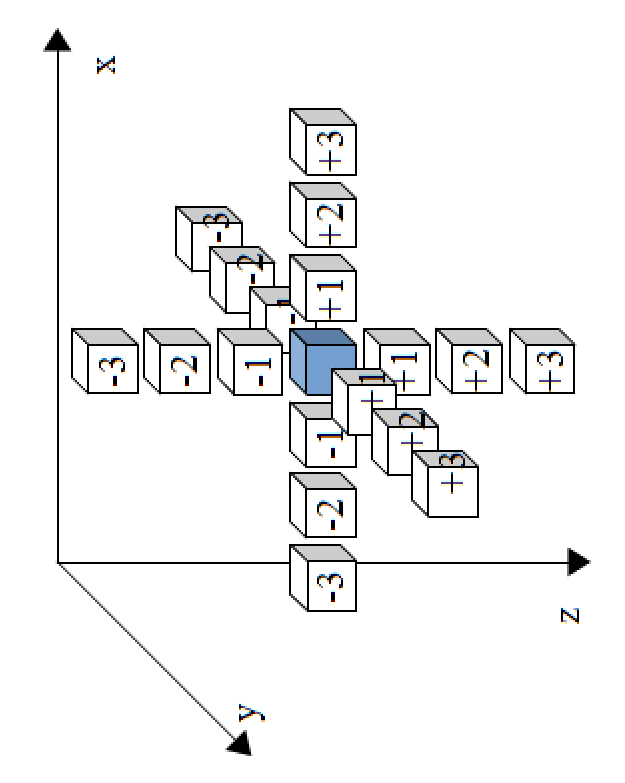
\includegraphics[angle=270,origin=b,width=0.60\textwidth]{fd6.eps}
\caption{Fd6}
\end{figure}

Here is a 19-point floating-point stencil calculation of degree 3. Calculate 24 rows by one burst operation (RMGRP = 24). Although it is a stencil calculation, mapdist = 0 because it calculates 24 lines at a time.

\begin{screen}
\tiny
\begin{verbatim}
fd6( float *c, float *b )
     /*C3D[DP][HT][WD]*/
     /*B3D[DP][HT][WD]*/
#define NCHIP     1
#define RMGRP     24
#define OMAP      1
#define PAD       3
#define RRANGE   ((HT-PAD*2)/NCHIP/OMAP)
  Ull  CHIP;
  Ull  LOOP1, LOOP0;
  Ull  INIT1, INIT0;
  Ull  AR[64][4];                     /* output of EX     in each unit */
  Ull  BR[64][4][4];                  /* output registers in each unit */
  Ull  r0, r1, r2, r3, r4, r5, r6, r7, r8, r9, r10, r11, r12, r13, r14, r15;
  Ull  r16, r17, r18, r19, r20, r21, r22, r23, r24, r25, r26, r27, r28, r29, r30, r31;
  Ull  cc0, cc1, cc2, cc3, ex0, ex1;
  int  x, y, z;
  int  row, col, n;
  Ull  roofs, coofs, aofs, bofs, cofs;
  union {float f; int i;} C1, C2, C3, C4;
  C1.f = 0.1;
  C2.f = 0.2;
  C3.f = 0.4;
  C4.f = 0.8;
  Ull  I1 = C1.i;
  Ull  I2 = C2.i;
  Ull  I3 = C3.i;
  Ull  I4 = C4.i;

#if !defined(EMAX5) && !defined(EMAX6)
  for (z=PAD; z<DP-PAD; z++) {
    for (y=PAD; y<HT-PAD; y++) {
      for (x=PAD; x<WD-PAD; x++) {
        *(c+z*WDHT+y*WD+x) = C4.f *(*(b+((z-3)*WDHT)+(y  )*WD+x  )
                                  + *(b+((z  )*WDHT)+(y-3)*WD+x  )
                                  + *(b+((z  )*WDHT)+(y  )*WD+x-3)
                                  + *(b+((z  )*WDHT)+(y  )*WD+x+3)
                                  + *(b+((z  )*WDHT)+(y+3)*WD+x  )
                                  + *(b+((z+3)*WDHT)+(y  )*WD+x  ))
                           + C3.f *(*(b+((z-2)*WDHT)+(y  )*WD+x  )
                                  + *(b+((z  )*WDHT)+(y-2)*WD+x  )
                                  + *(b+((z  )*WDHT)+(y  )*WD+x-2)
                                  + *(b+((z  )*WDHT)+(y  )*WD+x+2)
                                  + *(b+((z  )*WDHT)+(y+2)*WD+x  )
                                  + *(b+((z+2)*WDHT)+(y  )*WD+x  ))
                           + C2.f *(*(b+((z-1)*WDHT)+(y  )*WD+x  )
                                  + *(b+((z  )*WDHT)+(y-1)*WD+x  )
                                  + *(b+((z  )*WDHT)+(y  )*WD+x-1)
                                  + *(b+((z  )*WDHT)+(y  )*WD+x+1)
                                  + *(b+((z  )*WDHT)+(y+1)*WD+x  )
                                  + *(b+((z+1)*WDHT)+(y  )*WD+x  ))
                           + C1.f * *(b+((z  )*WDHT)+(y  )*WD+x  );
      }
    }
  }
#endif
\end{verbatim}
\end{screen}

\begin{screen}
\tiny
\begin{verbatim}
  for (z=PAD; z<DP-PAD; z++) {
    for (y=0; y<RRANGE; y+=RMGRP) {
      Ull  btop[NCHIP], ctop[NCHIP];
      Ull  brow00[NCHIP], brow01[NCHIP], brow02[NCHIP], brow03[NCHIP], brow04[NCHIP], brow05[NCHIP], brow06[NCHIP];
      Ull  brow07[NCHIP], brow08[NCHIP], brow09[NCHIP], brow0a[NCHIP], brow0b[NCHIP], brow0c[NCHIP];
      Ull  crow0[NCHIP];
      for (CHIP=0; CHIP<NCHIP; CHIP++) { /* output channels are parallelized by multi-chip (OC/#chip) */
        btop[CHIP]   = b               +(z  )*WDHT+(CHIP*RRANGE*OMAP+RRANGE*0+PAD+y  )*WD;
        ctop[CHIP]   = c               +(z  )*WDHT+(CHIP*RRANGE*OMAP+RRANGE*0+PAD+y  )*WD;
        brow00[CHIP] = b               +(z-3)*WDHT+(CHIP*RRANGE*OMAP+RRANGE*0+PAD+y  )*WD;
        brow01[CHIP] = b               +(z-2)*WDHT+(CHIP*RRANGE*OMAP+RRANGE*0+PAD+y  )*WD;
        brow02[CHIP] = b               +(z-1)*WDHT+(CHIP*RRANGE*OMAP+RRANGE*0+PAD+y  )*WD;
        brow03[CHIP] = b               +(z+1)*WDHT+(CHIP*RRANGE*OMAP+RRANGE*0+PAD+y  )*WD;
        brow04[CHIP] = b               +(z+2)*WDHT+(CHIP*RRANGE*OMAP+RRANGE*0+PAD+y  )*WD;
        brow05[CHIP] = b               +(z+3)*WDHT+(CHIP*RRANGE*OMAP+RRANGE*0+PAD+y  )*WD;
        brow06[CHIP] = b               +(z  )*WDHT+(CHIP*RRANGE*OMAP+RRANGE*0+PAD+y-3)*WD;
        brow07[CHIP] = b               +(z  )*WDHT+(CHIP*RRANGE*OMAP+RRANGE*0+PAD+y-2)*WD;/* not used for RMGRP>1 */
        brow08[CHIP] = b               +(z  )*WDHT+(CHIP*RRANGE*OMAP+RRANGE*0+PAD+y-1)*WD;/* not used for RMGRP>1 */
        brow09[CHIP] = b               +(z  )*WDHT+(CHIP*RRANGE*OMAP+RRANGE*0+PAD+y  )*WD;/* not used for RMGRP>1 */
        brow0a[CHIP] = b               +(z  )*WDHT+(CHIP*RRANGE*OMAP+RRANGE*0+PAD+y+1)*WD;/* not used for RMGRP>1 */
        brow0b[CHIP] = b               +(z  )*WDHT+(CHIP*RRANGE*OMAP+RRANGE*0+PAD+y+2)*WD;/* not used for RMGRP>1 */
        brow0c[CHIP] = b               +(z  )*WDHT+(CHIP*RRANGE*OMAP+RRANGE*0+PAD+y+3)*WD;/* not used for RMGRP>1 */
        crow0[CHIP]  = c               +(z  )*WDHT+(CHIP*RRANGE*OMAP+RRANGE*0+PAD+y  )*WD;
      }
//EMAX5A begin fd6 mapdist=0 /* 11 */
      for (CHIP=0; CHIP<NCHIP; CHIP++) { /* output channels are parallelized by multi-chip (OC/#chip) */
   /*2*/for (INIT1=1,LOOP1=RMGRP,roofs=0-WD*4; LOOP1--; INIT1=0) {      /* stage#0 *//* mapped to FOR() on BR[63][1][0] */
     /*1*/for (INIT0=1,LOOP0=WD-PAD*2,coofs=(PAD-1)*4; LOOP0--; INIT0=0) {          /* stage#0 *//* mapped to FOR() on BR[63][0][0] */
            exe(OP_ADD,  &coofs, INIT0?coofs:coofs, EXP_H3210, 4, EXP_H3210, 0LL, EXP_H3210, OP_AND, 0x00000000ffffffffLL, OP_NOP, 0LL); /* stage#0 */
            exe(OP_ADD,  &roofs, roofs,  EXP_H3210, INIT0?WD*4:0, EXP_H3210, 0LL, EXP_H3210, OP_AND, 0x00000000ffffffffLL, OP_NOP, 0LL); /* stage#0 */
            exe(OP_ADD3, &bofs,  btop[CHIP], EXP_H3210, roofs, EXP_H3210,  coofs, EXP_H3210, OP_AND, 0x000000ffffffffffLL, OP_NOP, 0LL); /* stage#1 */
            exe(OP_ADD3, &cofs,  ctop[CHIP], EXP_H3210, roofs, EXP_H3210,  coofs, EXP_H3210, OP_AND, 0x000000ffffffffffLL, OP_NOP, 0LL); /* stage#1 */
            /*map0*/
            mop(OP_LDWR, 1, &BR[2][0][1], bofs, (0        -WDHT*3   )*4, MSK_D0, brow00[CHIP], WD*RMGRP, 0, 0, NULL, WD*RMGRP); /* stage#2 */
            mop(OP_LDWR, 1, &BR[2][2][1], bofs, (0        +WDHT*3   )*4, MSK_D0, brow05[CHIP], WD*RMGRP, 0, 0, NULL, WD*RMGRP); /* stage#2 */
            exe(OP_FAD, &r3, BR[2][0][1],EXP_H3210,  BR[2][2][1], EXP_H3210, 0,          EXP_H3210, OP_NOP, 0LL, OP_NOP, 0LL);           /* stage#3 */
            mop(OP_LDWR, 1, &BR[3][0][1], bofs, (0        -WDHT*2   )*4, MSK_D0, brow01[CHIP], WD*RMGRP, 0, 0, NULL, WD*RMGRP); /* stage#3 */
            mop(OP_LDWR, 1, &BR[3][2][1], bofs, (0        +WDHT*2   )*4, MSK_D0, brow04[CHIP], WD*RMGRP, 0, 0, NULL, WD*RMGRP); /* stage#3 */
            exe(OP_FAD, &r2, BR[3][0][1],EXP_H3210,  BR[3][2][1], EXP_H3210, 0,          EXP_H3210, OP_NOP, 0LL, OP_NOP, 0LL);           /* stage#4 */
            mop(OP_LDWR, 1, &BR[4][0][1], bofs, (0        -WDHT*1   )*4, MSK_D0, brow02[CHIP], WD*RMGRP, 0, 0, NULL, WD*RMGRP); /* stage#4 */
            mop(OP_LDWR, 1, &BR[4][2][1], bofs, (0        +WDHT*1   )*4, MSK_D0, brow03[CHIP], WD*RMGRP, 0, 0, NULL, WD*RMGRP); /* stage#4 */
            exe(OP_FAD, &r1, BR[4][0][1],EXP_H3210,  BR[4][2][1], EXP_H3210, 0,          EXP_H3210, OP_NOP, 0LL, OP_NOP, 0LL);           /* stage#5 */
            mop(OP_LDWR, 1, &BR[5][0][1], bofs, (0             -WD*3)*4, MSK_D0, brow06[CHIP], WD*(RMGRP+PAD*2), 0, 0, NULL, WD*(RMGRP+PAD*2)); /* stage#5 */
            mop(OP_LDWR, 1, &BR[5][0][0], bofs, (0             +WD*3)*4, MSK_D0, brow06[CHIP], WD*(RMGRP+PAD*2), 0, 0, NULL, WD*(RMGRP+PAD*2)); /* stage#5 */
            mop(OP_LDWR, 1, &BR[5][1][1], bofs, (0                -3)*4, MSK_D0, brow06[CHIP], WD*(RMGRP+PAD*2), 0, 0, NULL, WD*(RMGRP+PAD*2)); /* stage#5 */
            mop(OP_LDWR, 1, &BR[5][1][0], bofs, (0                +3)*4, MSK_D0, brow06[CHIP], WD*(RMGRP+PAD*2), 0, 0, NULL, WD*(RMGRP+PAD*2)); /* stage#5 */
            exe(OP_FAD, &r13,BR[5][0][1],EXP_H3210,  BR[5][0][0], EXP_H3210, 0,          EXP_H3210, OP_NOP, 0LL, OP_NOP, 0LL);           /* stage#6 */
            exe(OP_FAD, &r23,BR[5][1][1],EXP_H3210,  BR[5][1][0], EXP_H3210, 0,          EXP_H3210, OP_NOP, 0LL, OP_NOP, 0LL);           /* stage#6 */
            mop(OP_LDWR, 1, &BR[6][0][1], bofs, (0             +WD*2)*4, MSK_D0, brow06[CHIP], WD*(RMGRP+PAD*2), 0, 0, NULL, WD*(RMGRP+PAD*2)); /* stage#6 */
            mop(OP_LDWR, 1, &BR[6][0][0], bofs, (0             -WD*2)*4, MSK_D0, brow06[CHIP], WD*(RMGRP+PAD*2), 0, 0, NULL, WD*(RMGRP+PAD*2)); /* stage#6 */
            mop(OP_LDWR, 1, &BR[6][1][1], bofs, (0                -2)*4, MSK_D0, brow06[CHIP], WD*(RMGRP+PAD*2), 0, 0, NULL, WD*(RMGRP+PAD*2)); /* stage#6 */
            mop(OP_LDWR, 1, &BR[6][1][0], bofs, (0                +2)*4, MSK_D0, brow06[CHIP], WD*(RMGRP+PAD*2), 0, 0, NULL, WD*(RMGRP+PAD*2)); /* stage#6 */
            exe(OP_FAD, &r12,BR[6][0][1],EXP_H3210,  BR[6][0][0], EXP_H3210, 0,          EXP_H3210, OP_NOP, 0LL, OP_NOP, 0LL);           /* stage#7 */
            exe(OP_FAD, &r22,BR[6][1][1],EXP_H3210,  BR[6][1][0], EXP_H3210, 0,          EXP_H3210, OP_NOP, 0LL, OP_NOP, 0LL);           /* stage#7 */
            exe(OP_FAD, &r23,r13,        EXP_H3210,  r23,         EXP_H3210, 0,          EXP_H3210, OP_NOP, 0LL, OP_NOP, 0LL);           /* stage#7 */
            mop(OP_LDWR, 1, &BR[7][0][1], bofs, (0             +WD*1)*4, MSK_D0, brow06[CHIP], WD*(RMGRP+PAD*2), 0, 0, NULL, WD*(RMGRP+PAD*2)); /* stage#7 */
            mop(OP_LDWR, 1, &BR[7][0][0], bofs, (0             -WD*1)*4, MSK_D0, brow06[CHIP], WD*(RMGRP+PAD*2), 0, 0, NULL, WD*(RMGRP+PAD*2)); /* stage#7 */
            mop(OP_LDWR, 1, &BR[7][1][1], bofs, (0                -1)*4, MSK_D0, brow06[CHIP], WD*(RMGRP+PAD*2), 0, 0, NULL, WD*(RMGRP+PAD*2)); /* stage#7 */
            mop(OP_LDWR, 1, &BR[7][1][0], bofs, (0                +1)*4, MSK_D0, brow06[CHIP], WD*(RMGRP+PAD*2), 0, 0, NULL, WD*(RMGRP+PAD*2)); /* stage#7 */
            exe(OP_FAD, &r11,BR[7][0][1],EXP_H3210,  BR[7][0][0], EXP_H3210, 0,          EXP_H3210, OP_NOP, 0LL, OP_NOP, 0LL);           /* stage#8 */
            exe(OP_FAD, &r21,BR[7][1][1],EXP_H3210,  BR[7][1][0], EXP_H3210, 0,          EXP_H3210, OP_NOP, 0LL, OP_NOP, 0LL);           /* stage#8 */
            exe(OP_FAD, &r22,r12,        EXP_H3210,  r22,         EXP_H3210, 0,          EXP_H3210, OP_NOP, 0LL, OP_NOP, 0LL);           /* stage#8 */
            exe(OP_FAD, &r3, r23,        EXP_H3210,  r3,          EXP_H3210, 0,          EXP_H3210, OP_NOP, 0LL, OP_NOP, 0LL);           /* stage#8 */
            mop(OP_LDWR, 1, &BR[8][0][1], bofs, (0                  )*4, MSK_D0, brow06[CHIP], WD*(RMGRP+PAD*2), 0, 0, NULL, WD*(RMGRP+PAD*2)); /* stage#8 */
            exe(OP_FML, &r10,BR[8][0][1],EXP_H3210,  I1,          EXP_H3210, 0,          EXP_H3210, OP_NOP, 0LL, OP_NOP, 0LL);           /* stage#9  */
            exe(OP_FAD, &r21,r11,        EXP_H3210,  r21,         EXP_H3210, 0,          EXP_H3210, OP_NOP, 0LL, OP_NOP, 0LL);           /* stage#9 */
            exe(OP_FAD, &r2, r22,        EXP_H3210,  r2,          EXP_H3210, 0,          EXP_H3210, OP_NOP, 0LL, OP_NOP, 0LL);           /* stage#9 */
            exe(OP_FMA, &r13,r10,        EXP_H3210,  r3,          EXP_H3210, I4,         EXP_H3210, OP_NOP, 0LL, OP_NOP, 0LL);           /* stage#10 */
            exe(OP_FAD, &r1, r21,        EXP_H3210,  r1,          EXP_H3210, 0,          EXP_H3210, OP_NOP, 0LL, OP_NOP, 0LL);           /* stage#10 */
            exe(OP_FMA, &r12,r13,        EXP_H3210,  r2,          EXP_H3210, I3,         EXP_H3210, OP_NOP, 0LL, OP_NOP, 0LL);           /* stage#11 */
            exe(OP_FMA, &r11,r12,        EXP_H3210,  r1,          EXP_H3210, I2,         EXP_H3210, OP_NOP, 0LL, OP_NOP, 0LL);           /* stage#12 */
            mop(OP_STWR, 3, &r11,        cofs, (0                   )*4, MSK_D0, crow0[CHIP],  WD*RMGRP, 0, 0, NULL, WD*RMGRP); /* stage#12 */
          }
        }
      }
//EMAX5A end
    }
//EMAX5A drain_dirty_lmm
  }
\end{verbatim}
\end{screen}

\begin{figure}[htbp]
\center
\epsfile{file=stencil+rmm-fd6-emax6.eps,width=1.00\textwidth}
\caption{Fd6}
\end{figure}

\clearpage

\subsection{Resid with stencil}

\begin{figure}[htbp]
\center
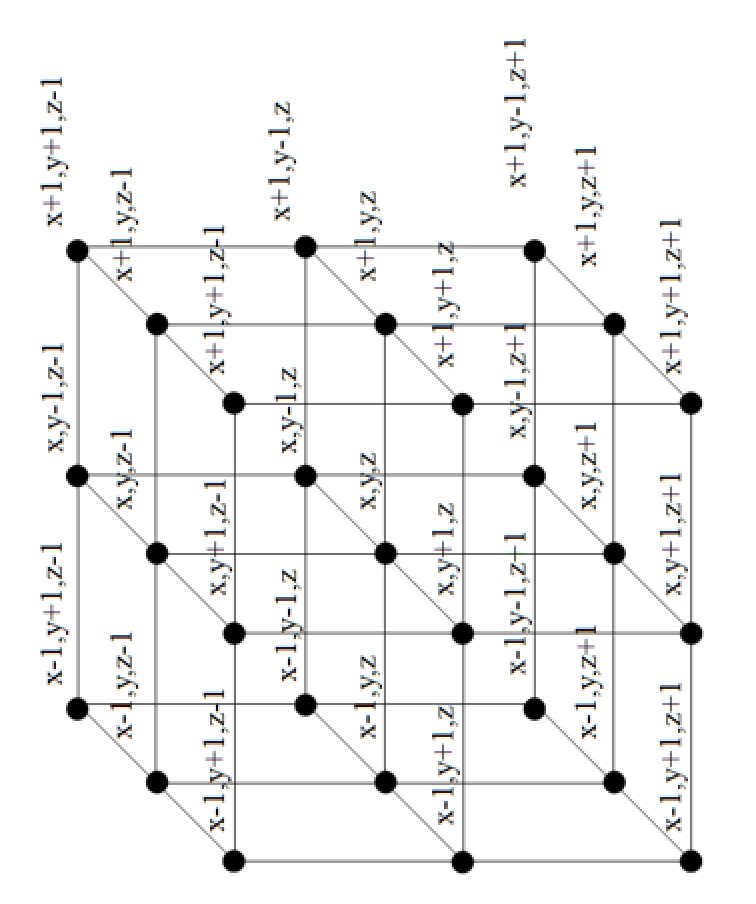
\includegraphics[angle=270,origin=b,width=0.65\textwidth]{resid.eps}
\caption{Resid}
\end{figure}

Here is a 27-point floating-point stencil calculation. Calculate 24 rows by one burst operation (RMGRP = 24). Although it is a stencil calculation, mapdist = 0 because it calculates 24 lines at a time.

\begin{screen}
\tiny
\begin{verbatim}
resid( float *d, float *b, float *c )
     /*D3D[DP][HT][WD]*/
     /*B3D[DP][HT][WD]*/
     /*C3D[DP][HT][WD]*/
#define NCHIP     1
#define RMGRP     24
#define OMAP      1
#define PAD       1
#define RRANGE   ((HT-PAD*2)/NCHIP/OMAP)
  Ull  CHIP;
  Ull  LOOP1, LOOP0;
  Ull  INIT1, INIT0;
  Ull  AR[64][4];                     /* output of EX     in each unit */
  Ull  BR[64][4][4];                  /* output registers in each unit */
  Ull  r0, r1, r2, r3, r4, r5, r6, r7, r8, r9, r10, r11, r12, r13, r14, r15;
  Ull  r16, r17, r18, r19, r20, r21, r22, r23, r24, r25, r26, r27, r28, r29, r30, r31;
  Ull  cc0, cc1, cc2, cc3, ex0, ex1;
  int  x, y, z;
  int  row, col, n;
  Ull  roofs, coofs, bofs, cofs, dofs;
  union {float f; int i;} A0, A1, A2, A3;
  A0.f = -0.1;  A1.f = -0.2;  A2.f = -0.3;  A3.f = -0.4;
  Ull  I0 = A0.i;  Ull  I1 = A1.i;  Ull  I2 = A2.i;  Ull  I3 = A3.i;

#if !defined(EMAX5) && !defined(EMAX6)
  for (z=PAD; z<DP-PAD; z++) {
    for (y=PAD; y<HT-PAD; y++) {
      for (x=PAD; x<WD-PAD; x++) {
        *(d+z*WDHT+y*WD+x) = *(c+z*WDHT+y*WD+x)
                    + A0.f * *(b+(z  )*WDHT+(y  )*WD+x  )
                    + A1.f *(*(b+(z-1)*WDHT+(y  )*WD+x  )
                           + *(b+(z  )*WDHT+(y-1)*WD+x  )
                           + *(b+(z  )*WDHT+(y  )*WD+x-1)
                           + *(b+(z  )*WDHT+(y  )*WD+x+1)
                           + *(b+(z  )*WDHT+(y+1)*WD+x  )
                           + *(b+(z+1)*WDHT+(y  )*WD+x  ))
                    + A2.f *(*(b+(z-1)*WDHT+(y-1)*WD+x  )
                           + *(b+(z-1)*WDHT+(y  )*WD+x-1)
                           + *(b+(z-1)*WDHT+(y  )*WD+x+1)
                           + *(b+(z-1)*WDHT+(y+1)*WD+x  )
                           + *(b+(z  )*WDHT+(y-1)*WD+x-1)
                           + *(b+(z  )*WDHT+(y-1)*WD+x+1)
                           + *(b+(z  )*WDHT+(y+1)*WD+x-1)
                           + *(b+(z  )*WDHT+(y+1)*WD+x+1)
                           + *(b+(z+1)*WDHT+(y-1)*WD+x  )
                           + *(b+(z+1)*WDHT+(y  )*WD+x-1)
                           + *(b+(z+1)*WDHT+(y  )*WD+x+1)
                           + *(b+(z+1)*WDHT+(y+1)*WD+x  ))
                    + A3.f *(*(b+(z-1)*WDHT+(y-1)*WD+x-1)
                           + *(b+(z-1)*WDHT+(y-1)*WD+x+1)
                           + *(b+(z-1)*WDHT+(y+1)*WD+x-1)
                           + *(b+(z-1)*WDHT+(y+1)*WD+x+1)
                           + *(b+(z+1)*WDHT+(y-1)*WD+x-1)
                           + *(b+(z+1)*WDHT+(y-1)*WD+x+1)
                           + *(b+(z+1)*WDHT+(y+1)*WD+x-1)
                           + *(b+(z+1)*WDHT+(y+1)*WD+x+1));
  } } }
#endif
\end{verbatim}
\end{screen}

\begin{screen}
\tiny
\begin{verbatim}
  for (z=PAD; z<DP-PAD; z++) {
    for (y=0; y<RRANGE; y+=RMGRP) {
      Ull  btop[NCHIP], ctop[NCHIP], dtop[NCHIP];
      Ull  brow00[NCHIP], brow01[NCHIP], brow02[NCHIP], brow03[NCHIP], brow04[NCHIP], brow05[NCHIP], brow06[NCHIP], brow07[NCHIP], brow08[NCHIP];
      Ull  crow0[NCHIP];
      Ull  drow0[NCHIP];
      for (CHIP=0; CHIP<NCHIP; CHIP++) { /* output channels are parallelized by multi-chip (OC/#chip) */
        btop[CHIP]   = b               +(z  )*WDHT+(CHIP*RRANGE*OMAP+RRANGE*0+PAD+y  )*WD;
        ctop[CHIP]   = c               +(z  )*WDHT+(CHIP*RRANGE*OMAP+RRANGE*0+PAD+y  )*WD;
        dtop[CHIP]   = d               +(z  )*WDHT+(CHIP*RRANGE*OMAP+RRANGE*0+PAD+y  )*WD;
        brow00[CHIP] = b               +(z-1)*WDHT+(CHIP*RRANGE*OMAP+RRANGE*0+PAD+y-1)*WD;
        brow01[CHIP] = b               +(z-1)*WDHT+(CHIP*RRANGE*OMAP+RRANGE*0+PAD+y  )*WD;/* not used for RMGRP>1 */
        brow02[CHIP] = b               +(z-1)*WDHT+(CHIP*RRANGE*OMAP+RRANGE*0+PAD+y+1)*WD;/* not used for RMGRP>1 */
        brow03[CHIP] = b               +(z  )*WDHT+(CHIP*RRANGE*OMAP+RRANGE*0+PAD+y-1)*WD;
        brow04[CHIP] = b               +(z  )*WDHT+(CHIP*RRANGE*OMAP+RRANGE*0+PAD+y  )*WD;/* not used for RMGRP>1 */
        brow05[CHIP] = b               +(z  )*WDHT+(CHIP*RRANGE*OMAP+RRANGE*0+PAD+y+1)*WD;/* not used for RMGRP>1 */
        brow06[CHIP] = b               +(z+1)*WDHT+(CHIP*RRANGE*OMAP+RRANGE*0+PAD+y-1)*WD;
        brow07[CHIP] = b               +(z+1)*WDHT+(CHIP*RRANGE*OMAP+RRANGE*0+PAD+y  )*WD;/* not used for RMGRP>1 */
        brow08[CHIP] = b               +(z+1)*WDHT+(CHIP*RRANGE*OMAP+RRANGE*0+PAD+y+1)*WD;/* not used for RMGRP>1 */
        crow0[CHIP]  = c               +(z  )*WDHT+(CHIP*RRANGE*OMAP+RRANGE*0+PAD+y  )*WD;
        drow0[CHIP]  = d               +(z  )*WDHT+(CHIP*RRANGE*OMAP+RRANGE*0+PAD+y  )*WD;
      }
//EMAX5A begin resid mapdist=0 /* 12 */
      for (CHIP=0; CHIP<NCHIP; CHIP++) { /* output channels are parallelized by multi-chip (OC/#chip) */
   /*2*/for (INIT1=1,LOOP1=RMGRP,roofs=0-WD*4; LOOP1--; INIT1=0) {      /* stage#0 *//* mapped to FOR() on BR[63][1][0] */
     /*1*/for (INIT0=1,LOOP0=WD-PAD*2,coofs=(PAD-1)*4; LOOP0--; INIT0=0) {          /* stage#0 *//* mapped to FOR() on BR[63][0][0] */
            exe(OP_ADD,  &coofs, INIT0?coofs:coofs, EXP_H3210, 4, EXP_H3210, 0LL, EXP_H3210, OP_AND, 0x00000000ffffffffLL, OP_NOP, 0LL); /* stage#0 */
            exe(OP_ADD,  &roofs, roofs,  EXP_H3210, INIT0?WD*4:0, EXP_H3210, 0LL, EXP_H3210, OP_AND, 0x00000000ffffffffLL, OP_NOP, 0LL); /* stage#0 */
            exe(OP_ADD3, &bofs,  btop[CHIP], EXP_H3210, roofs, EXP_H3210,  coofs, EXP_H3210, OP_AND, 0x000000ffffffffffLL, OP_NOP, 0LL); /* stage#1 */
            exe(OP_ADD3, &cofs,  ctop[CHIP], EXP_H3210, roofs, EXP_H3210,  coofs, EXP_H3210, OP_AND, 0x000000ffffffffffLL, OP_NOP, 0LL); /* stage#1 */
            exe(OP_ADD3, &dofs,  dtop[CHIP], EXP_H3210, roofs, EXP_H3210,  coofs, EXP_H3210, OP_AND, 0x000000ffffffffffLL, OP_NOP, 0LL); /* stage#1 */
            /*map0*/
            mop(OP_LDWR, 1, &BR[2][0][1], bofs, (0       -WDHT-WD-1)*4, MSK_D0, brow00[CHIP], WD*(RMGRP+PAD*2), 0, 0, NULL, WD*(RMGRP+PAD*2));/* stage#2 */
            mop(OP_LDWR, 1, &BR[2][0][0], bofs, (0       -WDHT-WD  )*4, MSK_D0, brow00[CHIP], WD*(RMGRP+PAD*2), 0, 0, NULL, WD*(RMGRP+PAD*2));/* stage#2 */
            mop(OP_LDWR, 1, &BR[2][1][1], bofs, (0       -WDHT-WD+1)*4, MSK_D0, brow00[CHIP], WD*(RMGRP+PAD*2), 0, 0, NULL, WD*(RMGRP+PAD*2));/* stage#2 */
            exe(OP_FML, &r0, BR[2][0][1], EXP_H3210,  I3,          EXP_H3210,  0,           EXP_H3210, OP_NOP, 0LL, OP_NOP, 0LL);      /* stage#3 */
            exe(OP_FML, &r1, BR[2][0][0], EXP_H3210,  I2,          EXP_H3210,  0,           EXP_H3210, OP_NOP, 0LL, OP_NOP, 0LL);      /* stage#3 */
            exe(OP_FML, &r2, BR[2][1][1], EXP_H3210,  I3,          EXP_H3210,  0,           EXP_H3210, OP_NOP, 0LL, OP_NOP, 0LL);      /* stage#3 */
            mop(OP_LDWR, 1, &BR[3][0][1], bofs, (0       -WDHT   -1)*4, MSK_D0, brow00[CHIP], WD*(RMGRP+PAD*2), 0, 0, NULL, WD*(RMGRP+PAD*2));/* stage#3 */
            mop(OP_LDWR, 1, &BR[3][0][0], bofs, (0       -WDHT     )*4, MSK_D0, brow00[CHIP], WD*(RMGRP+PAD*2), 0, 0, NULL, WD*(RMGRP+PAD*2));/* stage#3 */
            mop(OP_LDWR, 1, &BR[3][1][1], bofs, (0       -WDHT   +1)*4, MSK_D0, brow00[CHIP], WD*(RMGRP+PAD*2), 0, 0, NULL, WD*(RMGRP+PAD*2));/* stage#3 */
            exe(OP_FMA, &r3, r0,          EXP_H3210,  BR[3][0][1], EXP_H3210,  I2,          EXP_H3210, OP_NOP, 0LL, OP_NOP, 0LL);      /* stage#4 */
            exe(OP_FMA, &r4, r1,          EXP_H3210,  BR[3][0][0], EXP_H3210,  I1,          EXP_H3210, OP_NOP, 0LL, OP_NOP, 0LL);      /* stage#4 */
            exe(OP_FMA, &r5, r2,          EXP_H3210,  BR[3][1][1], EXP_H3210,  I2,          EXP_H3210, OP_NOP, 0LL, OP_NOP, 0LL);      /* stage#4 */
            mop(OP_LDWR, 1, &BR[4][0][1], bofs, (0       -WDHT+WD-1)*4, MSK_D0, brow00[CHIP], WD*(RMGRP+PAD*2), 0, 0, NULL, WD*(RMGRP+PAD*2));/* stage#4 */
            mop(OP_LDWR, 1, &BR[4][0][0], bofs, (0       -WDHT+WD  )*4, MSK_D0, brow00[CHIP], WD*(RMGRP+PAD*2), 0, 0, NULL, WD*(RMGRP+PAD*2));/* stage#4 */
            mop(OP_LDWR, 1, &BR[4][1][1], bofs, (0       -WDHT+WD+1)*4, MSK_D0, brow00[CHIP], WD*(RMGRP+PAD*2), 0, 0, NULL, WD*(RMGRP+PAD*2));/* stage#4 */
            exe(OP_FMA, &r6, r3,          EXP_H3210,  BR[4][0][1], EXP_H3210,  I3,          EXP_H3210, OP_NOP, 0LL, OP_NOP, 0LL);      /* stage#5 */
            exe(OP_FMA, &r7, r4,          EXP_H3210,  BR[4][0][0], EXP_H3210,  I2,          EXP_H3210, OP_NOP, 0LL, OP_NOP, 0LL);      /* stage#5 */
            exe(OP_FMA, &r8, r5,          EXP_H3210,  BR[4][1][1], EXP_H3210,  I3,          EXP_H3210, OP_NOP, 0LL, OP_NOP, 0LL);      /* stage#5 */

            mop(OP_LDWR, 1, &BR[5][0][1], bofs, (0            -WD-1)*4, MSK_D0, brow03[CHIP], WD*(RMGRP+PAD*2), 0, 0, NULL, WD*(RMGRP+PAD*2));/* stage#5 */
            mop(OP_LDWR, 1, &BR[5][0][0], bofs, (0            -WD  )*4, MSK_D0, brow03[CHIP], WD*(RMGRP+PAD*2), 0, 0, NULL, WD*(RMGRP+PAD*2));/* stage#5 */
            mop(OP_LDWR, 1, &BR[5][1][1], bofs, (0            -WD+1)*4, MSK_D0, brow03[CHIP], WD*(RMGRP+PAD*2), 0, 0, NULL, WD*(RMGRP+PAD*2));/* stage#5 */
            exe(OP_FMA, &r0, r6,          EXP_H3210,  BR[5][0][1], EXP_H3210,  I2,          EXP_H3210, OP_NOP, 0LL, OP_NOP, 0LL);      /* stage#6 */
            exe(OP_FMA, &r1, r7,          EXP_H3210,  BR[5][0][0], EXP_H3210,  I1,          EXP_H3210, OP_NOP, 0LL, OP_NOP, 0LL);      /* stage#6 */
            exe(OP_FMA, &r2, r8,          EXP_H3210,  BR[5][1][1], EXP_H3210,  I2,          EXP_H3210, OP_NOP, 0LL, OP_NOP, 0LL);      /* stage#6 */
            mop(OP_LDWR, 1, &BR[6][0][1], bofs, (0               -1)*4, MSK_D0, brow03[CHIP], WD*(RMGRP+PAD*2), 0, 0, NULL, WD*(RMGRP+PAD*2));/* stage#6 */
            mop(OP_LDWR, 1, &BR[6][0][0], bofs, (0                 )*4, MSK_D0, brow03[CHIP], WD*(RMGRP+PAD*2), 0, 0, NULL, WD*(RMGRP+PAD*2));/* stage#6 */
            mop(OP_LDWR, 1, &BR[6][1][1], bofs, (0               +1)*4, MSK_D0, brow03[CHIP], WD*(RMGRP+PAD*2), 0, 0, NULL, WD*(RMGRP+PAD*2));/* stage#6 */
            exe(OP_FMA, &r3, r0,          EXP_H3210,  BR[6][0][1], EXP_H3210,  I1,          EXP_H3210, OP_NOP, 0LL, OP_NOP, 0LL);      /* stage#7 */
            exe(OP_FMA, &r4, r1,          EXP_H3210,  BR[6][0][0], EXP_H3210,  I0,          EXP_H3210, OP_NOP, 0LL, OP_NOP, 0LL);      /* stage#7 */
            exe(OP_FMA, &r5, r2,          EXP_H3210,  BR[6][1][1], EXP_H3210,  I1,          EXP_H3210, OP_NOP, 0LL, OP_NOP, 0LL);      /* stage#7 */
            mop(OP_LDWR, 1, &BR[7][0][1], bofs, (0            +WD-1)*4, MSK_D0, brow03[CHIP], WD*(RMGRP+PAD*2), 0, 0, NULL, WD*(RMGRP+PAD*2));/* stage#7 */
            mop(OP_LDWR, 1, &BR[7][0][0], bofs, (0            +WD  )*4, MSK_D0, brow03[CHIP], WD*(RMGRP+PAD*2), 0, 0, NULL, WD*(RMGRP+PAD*2));/* stage#7 */
            mop(OP_LDWR, 1, &BR[7][1][1], bofs, (0            +WD+1)*4, MSK_D0, brow03[CHIP], WD*(RMGRP+PAD*2), 0, 0, NULL, WD*(RMGRP+PAD*2));/* stage#7 */
            exe(OP_FMA, &r6, r3,          EXP_H3210,  BR[7][0][1], EXP_H3210,  I2,          EXP_H3210, OP_NOP, 0LL, OP_NOP, 0LL);      /* stage#8 */
            exe(OP_FMA, &r7, r4,          EXP_H3210,  BR[7][0][0], EXP_H3210,  I1,          EXP_H3210, OP_NOP, 0LL, OP_NOP, 0LL);      /* stage#8 */
            exe(OP_FMA, &r8, r5,          EXP_H3210,  BR[7][1][1], EXP_H3210,  I2,          EXP_H3210, OP_NOP, 0LL, OP_NOP, 0LL);      /* stage#8 */

            mop(OP_LDWR, 1, &BR[8][0][1], bofs, (0       +WDHT-WD-1)*4, MSK_D0, brow06[CHIP], WD*(RMGRP+PAD*2), 0, 0, NULL, WD*(RMGRP+PAD*2));/* stage#8 */
            mop(OP_LDWR, 1, &BR[8][0][0], bofs, (0       +WDHT-WD  )*4, MSK_D0, brow06[CHIP], WD*(RMGRP+PAD*2), 0, 0, NULL, WD*(RMGRP+PAD*2));/* stage#8 */
            mop(OP_LDWR, 1, &BR[8][1][1], bofs, (0       +WDHT-WD+1)*4, MSK_D0, brow06[CHIP], WD*(RMGRP+PAD*2), 0, 0, NULL, WD*(RMGRP+PAD*2));/* stage#8 */
            exe(OP_FMA, &r0, r6,          EXP_H3210,  BR[8][0][1], EXP_H3210,  I3,          EXP_H3210, OP_NOP, 0LL, OP_NOP, 0LL);      /* stage#9 */
            exe(OP_FMA, &r1, r7,          EXP_H3210,  BR[8][0][0], EXP_H3210,  I2,          EXP_H3210, OP_NOP, 0LL, OP_NOP, 0LL);      /* stage#9 */
            exe(OP_FMA, &r2, r8,          EXP_H3210,  BR[8][1][1], EXP_H3210,  I3,          EXP_H3210, OP_NOP, 0LL, OP_NOP, 0LL);      /* stage#9 */
            mop(OP_LDWR, 1, &BR[9][0][1], bofs, (0       +WDHT   -1)*4, MSK_D0, brow06[CHIP], WD*(RMGRP+PAD*2), 0, 0, NULL, WD*(RMGRP+PAD*2));/* stage#9 */
            mop(OP_LDWR, 1, &BR[9][0][0], bofs, (0       +WDHT     )*4, MSK_D0, brow06[CHIP], WD*(RMGRP+PAD*2), 0, 0, NULL, WD*(RMGRP+PAD*2));/* stage#9 */
            mop(OP_LDWR, 1, &BR[9][1][1], bofs, (0       +WDHT   +1)*4, MSK_D0, brow06[CHIP], WD*(RMGRP+PAD*2), 0, 0, NULL, WD*(RMGRP+PAD*2));/* stage#9 */
            exe(OP_FMA, &r3, r0,          EXP_H3210,  BR[9][0][1], EXP_H3210,  I2,          EXP_H3210, OP_NOP, 0LL, OP_NOP, 0LL);      /* stage#10*/
            exe(OP_FMA, &r4, r1,          EXP_H3210,  BR[9][0][0], EXP_H3210,  I1,          EXP_H3210, OP_NOP, 0LL, OP_NOP, 0LL);      /* stage#10*/
            exe(OP_FMA, &r5, r2,          EXP_H3210,  BR[9][1][1], EXP_H3210,  I2,          EXP_H3210, OP_NOP, 0LL, OP_NOP, 0LL);      /* stage#10*/
            mop(OP_LDWR, 1, &BR[10][0][1],bofs, (0       +WDHT+WD-1)*4, MSK_D0, brow06[CHIP], WD*(RMGRP+PAD*2), 0, 0, NULL, WD*(RMGRP+PAD*2));/* stage#10*/
            mop(OP_LDWR, 1, &BR[10][0][0],bofs, (0       +WDHT+WD  )*4, MSK_D0, brow06[CHIP], WD*(RMGRP+PAD*2), 0, 0, NULL, WD*(RMGRP+PAD*2));/* stage#10*/
            mop(OP_LDWR, 1, &BR[10][1][1],bofs, (0       +WDHT+WD+1)*4, MSK_D0, brow06[CHIP], WD*(RMGRP+PAD*2), 0, 0, NULL, WD*(RMGRP+PAD*2));/* stage#10*/
            exe(OP_FMA, &r6, r3,          EXP_H3210,  BR[10][0][1],EXP_H3210,  I3,          EXP_H3210, OP_NOP, 0LL, OP_NOP, 0LL);      /* stage#11*/
            exe(OP_FMA, &r7, r4,          EXP_H3210,  BR[10][0][0],EXP_H3210,  I2,          EXP_H3210, OP_NOP, 0LL, OP_NOP, 0LL);      /* stage#11*/
            exe(OP_FMA, &r8, r5,          EXP_H3210,  BR[10][1][1],EXP_H3210,  I3,          EXP_H3210, OP_NOP, 0LL, OP_NOP, 0LL);      /* stage#11*/
            mop(OP_LDWR, 1, &BR[11][0][1],cofs, (0                 )*4, MSK_D0, crow0[CHIP],  WD*RMGRP, 0, 0, NULL, WD*RMGRP);     /* stage#11*/
            exe(OP_FAD, &r1, r6,          EXP_H3210,  BR[11][0][1],EXP_H3210,  0,           EXP_H3210, OP_NOP, 0LL, OP_NOP, 0LL);      /* stage#12*/
            exe(OP_FAD, &r2, r7,          EXP_H3210,  r8,          EXP_H3210,  0,           EXP_H3210, OP_NOP, 0LL, OP_NOP, 0LL);      /* stage#12*/
            exe(OP_FAD, &r0, r1,          EXP_H3210,  r2,          EXP_H3210,  0,           EXP_H3210, OP_NOP, 0LL, OP_NOP, 0LL);      /* stage#13*/
            mop(OP_STWR, 3, &r0,          dofs, (0                 )*4, MSK_D0, drow0[CHIP],  WD*RMGRP, 0, 0, NULL, WD*RMGRP);     /* stage#13*/
          }
        }
      }
//EMAX5A end
    }
//EMAX5A drain_dirty_lmm
  }
\end{verbatim}
\end{screen}

\begin{figure}[htbp]
\center
\epsfile{file=stencil+rmm-resid-emax6.eps,width=1.00\textwidth}
\caption{Resid}
\end{figure}

\clearpage

\subsection{Wave2d with stencil}

\begin{figure}[htbp]
\center
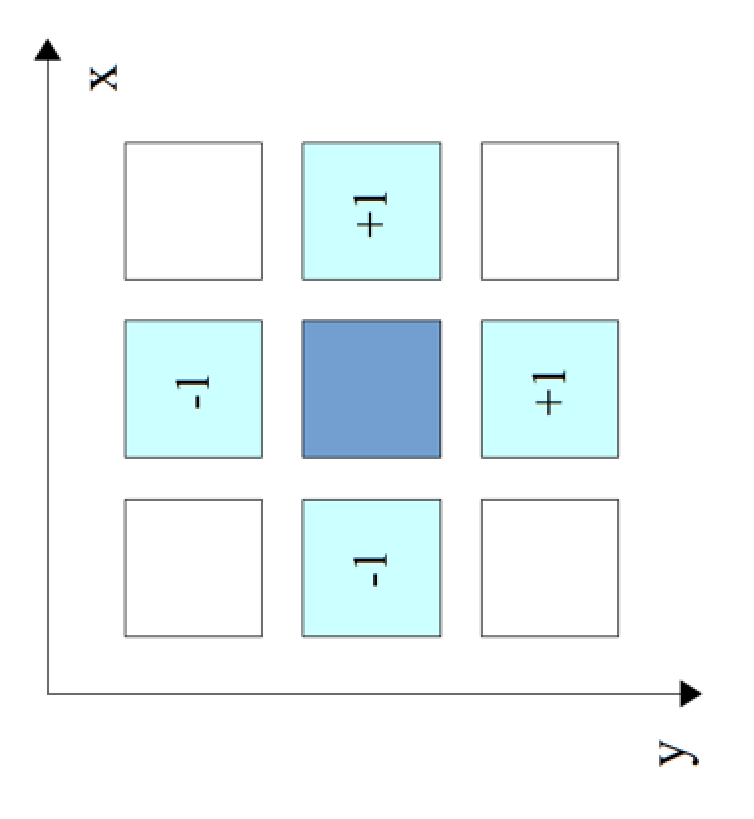
\includegraphics[angle=270,origin=b,width=0.60\textwidth]{wave2d.eps}
\caption{Wave2d}
\end{figure}

Here is a 5-point floating-point stencil calculation.
Calculate 24 rows by one burst operation (RMGRP = 24). Although it is a stencil calculation, mapdist = 0 because it calculates 24 lines at a time.
Performance can be improved by PLOAD using unused stages. However, if PAD> 1, the AXI transaction for PLOAD also hits the LOAD target LMM because the areas of the LOAD target LMM and the PLOAD target LMM partially overlap. AXI is waited in the load cycle, and AXI may be congested.

\begin{screen}
\tiny
\begin{verbatim}
wave2d( float *z2, float *z0, float *z1 )
     /*WZ2[HT][WD]*/
     /*WZ0[HT][WD]*/
     /*WZ1[HT][WD]*/
#define NCHIP     1
#define RMGRP     24
#define OMAP      1
#define PAD       1
#define RRANGE   ((HT-PAD*2)/NCHIP/OMAP)
  Ull  CHIP;
  Ull  LOOP1, LOOP0;
  Ull  INIT1, INIT0;
  Ull  AR[64][4];                     /* output of EX     in each unit */
  Ull  BR[64][4][4];                  /* output registers in each unit */
  Ull  r0, r1, r2, r3, r4, r5, r6, r7, r8, r9, r10, r11, r12, r13, r14, r15;
  Ull  r16, r17, r18, r19, r20, r21, r22, r23, r24, r25, r26, r27, r28, r29, r30, r31;
  Ull  cc0, cc1, cc2, cc3, ex0, ex1;
  int  x, y, z;
  int  row, col, n;
  Ull  roofs, coofs, z0ofs, z1ofs, z2ofs;
  union {float f; int i;} C1, C2, C3, C4;
  C1.f =  2.00;
  C2.f = -1.00;
  C3.f =  0.25;
  C4.f = -4.00;
  Ull  I1 = C1.i;
  Ull  I2 = C2.i;
  Ull  I3 = C3.i;
  Ull  I4 = C4.i;

#if !defined(EMAX5) && !defined(EMAX6)
  for (y=PAD; y<HT-PAD; y++) {
    for (x=PAD; x<WD-PAD; x++) {
      *(z2+y*WD+x) =  C1.f * *(z1+y*WD+x)
                   +  C2.f * *(z0+y*WD+x)
                   +  C3.f *(*(z1+(y+1)*WD+x  )
                           + *(z1+(y-1)*WD+x  )
                           + *(z1+(y  )*WD+x-1)
                           + *(z1+(y  )*WD+x+1) + C4.f * *(z1+y*WD+x));
    }
  }
#endif
\end{verbatim}
\end{screen}

\begin{screen}
\tiny
\begin{verbatim}
  for (y=0; y<RRANGE; y+=RMGRP) {
    Ull  z0top[NCHIP], z1top[NCHIP], z2top[NCHIP];
    Ull  z0row0[NCHIP];
    Ull  z1row00[NCHIP], z1row01[NCHIP], z1row02[NCHIP];
    Ull  z2row0[NCHIP];
    for (CHIP=0; CHIP<NCHIP; CHIP++) { /* output channels are parallelized by multi-chip (OC/#chip) */
      z0top[CHIP]   = z0              +(CHIP*RRANGE*OMAP+RRANGE*0+PAD+y  )*WD;
      z1top[CHIP]   = z1              +(CHIP*RRANGE*OMAP+RRANGE*0+PAD+y  )*WD;
      z2top[CHIP]   = z2              +(CHIP*RRANGE*OMAP+RRANGE*0+PAD+y  )*WD;
      z0row0[CHIP]  = z0              +(CHIP*RRANGE*OMAP+RRANGE*0+PAD+y  )*WD;
      z1row00[CHIP] = z1              +(CHIP*RRANGE*OMAP+RRANGE*0+PAD+y-1)*WD;
      z1row01[CHIP] = z1              +(CHIP*RRANGE*OMAP+RRANGE*0+PAD+y  )*WD;/* not used for RMGRP>1 */
      z1row02[CHIP] = z1              +(CHIP*RRANGE*OMAP+RRANGE*0+PAD+y+1)*WD;/* not used for RMGRP>1 */
      z2row0[CHIP]  = z2              +(CHIP*RRANGE*OMAP+RRANGE*0+PAD+y  )*WD;
    }
//EMAX5A begin wave2d mapdist=0 /* 8 */
    for (CHIP=0; CHIP<NCHIP; CHIP++) { /* output channels are parallelized by multi-chip (OC/#chip) */
 /*2*/for (INIT1=1,LOOP1=RMGRP,roofs=0-WD*4; LOOP1--; INIT1=0) {      /* stage#0 *//* mapped to FOR() on BR[63][1][0] */
   /*1*/for (INIT0=1,LOOP0=WD-PAD*2,coofs=(PAD-1)*4; LOOP0--; INIT0=0) {          /* stage#0 *//* mapped to FOR() on BR[63][0][0] */
          exe(OP_ADD,  &coofs, INIT0?coofs:coofs, EXP_H3210, 4, EXP_H3210,  0LL, EXP_H3210, OP_AND, 0x00000000ffffffffLL, OP_NOP, 0LL); /* stage#0 */
          exe(OP_ADD,  &roofs, roofs,  EXP_H3210, INIT0?WD*4:0, EXP_H3210,  0LL, EXP_H3210, OP_AND, 0x00000000ffffffffLL, OP_NOP, 0LL); /* stage#0 */
          exe(OP_ADD3, &z0ofs, z0top[CHIP], EXP_H3210, roofs, EXP_H3210,  coofs, EXP_H3210, OP_AND, 0x000000ffffffffffLL, OP_NOP, 0LL); /* stage#1 */
          exe(OP_ADD3, &z1ofs, z1top[CHIP], EXP_H3210, roofs, EXP_H3210,  coofs, EXP_H3210, OP_AND, 0x000000ffffffffffLL, OP_NOP, 0LL); /* stage#1 */
          exe(OP_ADD3, &z2ofs, z2top[CHIP], EXP_H3210, roofs, EXP_H3210,  coofs, EXP_H3210, OP_AND, 0x000000ffffffffffLL, OP_NOP, 0LL); /* stage#1 */
          /*map0*/
          mop(OP_LDWR, 1, &BR[2][0][1], z0ofs, (0                  )*4, MSK_D0, z0row0[CHIP],  WD*RMGRP, 0, 0, NULL, WD*RMGRP);  /* stage#2 */
          exe(OP_FML, &r0, BR[2][0][1], EXP_H3210,  I2,          EXP_H3210,  0,           EXP_H3210, OP_NOP, 0LL, OP_NOP, 0LL);      /* stage#3 */
          mop(OP_LDWR, 1, &BR[3][0][1], z1ofs, (0             -WD  )*4, MSK_D0, z1row00[CHIP], WD*(RMGRP+PAD*2), 0, 0, NULL, WD*(RMGRP+PAD*2)); /* stage#3 */
          mop(OP_LDWR, 1, &BR[4][0][1], z1ofs, (0                -1)*4, MSK_D0, z1row00[CHIP], WD*(RMGRP+PAD*2), 0, 0, NULL, WD*(RMGRP+PAD*2)); /* stage#4 */
          mop(OP_LDWR, 1, &BR[4][0][0], z1ofs, (0                  )*4, MSK_D0, z1row00[CHIP], WD*(RMGRP+PAD*2), 0, 0, NULL, WD*(RMGRP+PAD*2)); /* stage#4 */
          mop(OP_LDWR, 1, &BR[4][1][1], z1ofs, (0                +1)*4, MSK_D0, z1row00[CHIP], WD*(RMGRP+PAD*2), 0, 0, NULL, WD*(RMGRP+PAD*2)); /* stage#4 */
          exe(OP_FAD, &r1, BR[3][0][1], EXP_H3210,  BR[4][0][1], EXP_H3210,  0,           EXP_H3210, OP_NOP, 0LL, OP_NOP, 0LL);      /* stage#5 */
          mop(OP_LDWR, 1, &BR[5][0][1], z1ofs, (0             +WD  )*4, MSK_D0, z1row00[CHIP], WD*(RMGRP+PAD*2), 0, 0, NULL, WD*(RMGRP+PAD*2)); /* stage#5 */
          exe(OP_FMA, &r2, r1,          EXP_H3210,  BR[4][0][0], EXP_H3210,  I4,          EXP_H3210, OP_NOP, 0LL, OP_NOP, 0LL);      /* stage#6 */
          exe(OP_FAD, &r3, BR[4][1][1], EXP_H3210,  BR[5][0][1], EXP_H3210,  0,           EXP_H3210, OP_NOP, 0LL, OP_NOP, 0LL);      /* stage#6 */
          exe(OP_FAD, &r4, r2,          EXP_H3210,  r3,          EXP_H3210,  0,           EXP_H3210, OP_NOP, 0LL, OP_NOP, 0LL);      /* stage#7 */
          exe(OP_FMA, &r5, r0,          EXP_H3210,  r4,          EXP_H3210,  I3,          EXP_H3210, OP_NOP, 0LL, OP_NOP, 0LL);      /* stage#8 */
          exe(OP_FMA, &r6, r5,          EXP_H3210,  BR[4][0][0], EXP_H3210,  I1,          EXP_H3210, OP_NOP, 0LL, OP_NOP, 0LL);      /* stage#9 */
          mop(OP_STWR, 3, &r6,          z2ofs, (0                  )*4, MSK_D0, z2row0[CHIP],  WD*RMGRP, 0, 0, NULL, WD*RMGRP);  /* stage#9 */
        }
      }
    }
//EMAX5A end
  }
//EMAX5A drain_dirty_lmm
\end{verbatim}
\end{screen}

\begin{figure}[htbp]
\center
\epsfile{file=stencil+rmm-wave2d-emax6.eps,width=1.00\textwidth}
\caption{Wave2d}
\end{figure}

\clearpage

\section{Practical kernel}

\subsection{3x3 Convolution}

\shabox{
\leftline{cent\% make -f Makefile-csim.emax6+dma cnn-csim.emax6+dma clean}
\leftline{cent\% ../../src/csim/csim -x cnn-csim.emax6+dma}
}

\shabox{
\leftline{zynq\% make -f Makefile-zynq.emax6+dma cnn-zynq.emax6+dma clean}
\leftline{zynq\% ./cnn-zynq.emax6+dma}
}

\begin{figure}[htbp]
\center
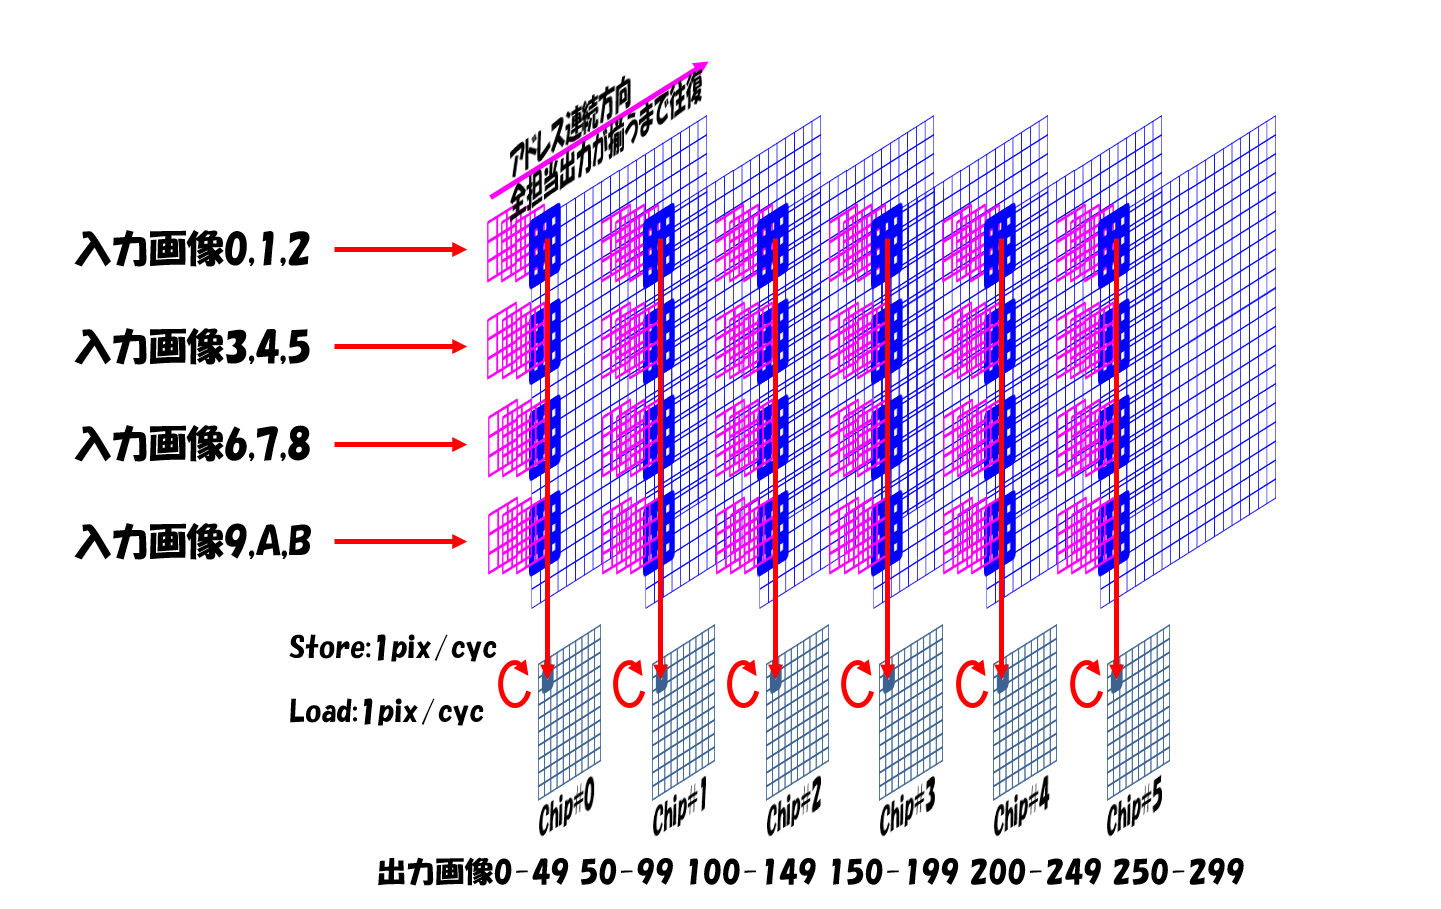
\includegraphics[angle=270,origin=b,width=0.90\textwidth]{EMAX6CNN.eps}
\caption{\label{cnn}CNN mapping}
\end{figure}

Figure \ref {cnn} shows the data flow in the convolution operation (CNN) of
Alexnet, one of the application programs. It finds the product-sum result of
a part of the input image and the kernel (weight). The sum of
multiple-direction input images is used as part of the output image (All
input images are needed to get one output image). The number of pixels in
each input image gradually decreases, and the number of images
increases. Since the output image of this process will become the input
image for the next process, the number of input images always be equal or
less than the number of output images.  Because all images cannot be stored
in hardware at the same time, a suitable hardware configuration must be able
to: broadcast the input image sequentially, divide the operation into output
image units, and accumulate the next output value in the output image.

\begin{figure}[htbp]
\center

\includegraphics[width=0.98\textwidth]{cnn0.eps}
\caption{\label{fig:cnn0}Cnn}
\end{figure}

This is a 242 x 242 convolution operation. Eight rows are calculated by one
burst operation (RMGRP = 8). Although it is a stencil calculation, mapdist =
0 because 8 lines are calculated at a time.  Figure \ref {fig:cnn0} (a)
shows the CNN data structure, and (b) shows a (K$^2$ + 1)xW CGRA with one
multiply-accumulate unit in each unit (Assuming M$\ge$K, OC$\ge$W). (b)
shows a data flow graph, not a snapshot at the same time, for simplicity. In
the actual hardware, the data in each stage is as shown in Figure \ref
{fig:mm0} (c). Data is pipelined.  The CNN accumulates the sum of products
of a part of input in (KxK) and kernel (KxK) for all input channels and
stores it in output signal out.  The total number of input words is
M$^2$xIC, the total number of words in the kernel is K$^2$xICxOC (which is
obtained by multiplying K$^2$ by the number of input channels (IC) and the
number of output channels (OC). The total number of words in the output is
M$^2$xOC.  K used for CNN is odd number in order to correspond to the even
number of hardware parameter W, and decrease the operation rate of
calculation units. The KxK multiply-accumulate operation is pipelined in
correspondence with one column of unit [*] [oc mod W], and when W output
channels are calculated simultaneously, all K$^2$xW arithmetic units can be
used (However, a broadcast function for K-stage LMM is required).  (c)
further divides OC into N chips, performs parallel processing, and each chip
has a number of K$^2$ stages of product-sum operation that can be mapped to
REP pairs x W columns. This is an implementation that can accommodate rows
(M elements) x GRP rows and all kernels (IC*OC*K*K elements).  The
seven loops in the rectangle correspond to the process of starting the CGRA
of all chips once. Each iteration of the chip loop corresponds to the
process of calculating the output channels of W groups by GRP rows by
convolution of the input channels of REP pairs and the kernel in each chip.
While the outer loop \textbf{oc} increases from 0 to OC/N-1, the LMM except
for the last stage of each chip holds in for GRP rows. On the other hand,
the last stage LMM needs to be replaced every time \textbf{oc} is updated.
The theoretical number of cycles required for the above operation will be
K$^2$x(M-2)$^2$xICxOC/(K$^2$xREPxWxN) = (M-2)$^2$xICxOC/(REPxWxN), if
excluding the CGRA starting time ��K$^2$xREP cycles�� and LMM replacement
time.  In addition, the theoretical DDR-LMM transfer amount when the LMM can
accommodate all of in, kernel, and out will be: M$^2$xIC + K$^2$xICxOC +
M$^2$xOC.  When each LMM can accommodate only MxGRP in, MxGRPxW out, and
only kernel, the transfer amount of in and kernel will be: M$^2$xIC and
K$^2$xICxOC. Since the number of rotations outside the rectangle (OC/N/W) x
(IC/REP) x (M /GRP) multiplied by N occurs, it will be M$^2$x2xOCxIC/REP (In
the case of IC = REP, out can be calculated at once and no replacement is
required, so M$^2$xOC of only DDR output. Independent of N).

\begin{screen}
\tiny
\begin{verbatim}
orig() {
  for (ic=0; ic<IC; ic++) { /* set input channel */
    ip0 = &in[ic*M*M]; /* top of input */
    for (row=1; row<M-1; row++) { /* image loop */
      for (col=1; col<M-1; col++) {
        for (oc=0; oc<OC; oc++) { /* set output channel */
          op = &out0[oc*M*M+row*M+col]; /* top of output */
          kp = &ker[(oc*IC+ic)*K*K];
          kidx = 0;
          for (y=-((K-1)/2); y<=(K-1)/2; y++) { /* kernel loop */
            for (x=-((K-1)/2); x<=(K-1)/2; x++) {
              if (ic == 0 && kidx == 0) {
                *(float*)&*op  = *(float*)&ip0[(row+y)*M+col+x] * *(float*)&kp[kidx];
              }
              else {
                *(float*)&*op += *(float*)&ip0[(row+y)*M+col+x] * *(float*)&kp[kidx];
              }
              kidx++;
              count0++;
} } } } } } }
\end{verbatim}
\end{screen}

\begin{screen}
\tiny
\begin{verbatim}
imax() {
  Ull CHIP;
  Ull rofs;
  for (top=1; top<M-1; top+=RMGRP) {
    for (iset=0; iset<IC; iset+=IMAP) { /* accumulate multiple sets of IC */
      for (oc=0; oc<OC/NCHIP; oc+=W) { /* set output channel */
  /*3*/ for (CHIP=0; CHIP<NCHIP; CHIP++) { /* output channels are parallelized by multi-chip (OC/#chip) */
    /*2*/ for (rofs=0; rofs<RMGRP; rofs++) { /* image loop (row) */
      /*1*/ for (col=1; col<M-1; col++) { /* image loop (col) */
              for (w=0; w<W; w++) { /* set output channel */
                op = &out1[(CHIP*OC/NCHIP+oc+w)*M*M+(top+rofs)*M+col]; /* top of output */
                for (ic=0; ic<IMAP; ic++) { /* set offset of input channel */
                  ip0 = &in[(iset+ic)*M*M]; /* top of input */
                  kp = &ker[((CHIP*OC/NCHIP+oc+w)*IC+iset+ic)*K*K];
                  kidx = 0;
                  for (y=-((K-1)/2); y<=(K-1)/2; y++) { /* kernel loop */
                    for (x=-((K-1)/2); x<=(K-1)/2; x++) {
                      if (iset == 0 && ic == 0 && kidx == 0) {
                        *(float*)&*op  = *(float*)&ip0[(top+rofs+y)*M+col+x] * *(float*)&kp[kidx];
                      }
                      else {
                        *(float*)&*op += *(float*)&ip0[(top+rofs+y)*M+col+x] * *(float*)&kp[kidx];
                      }
                      kidx++;
                      count1++;
} } } } } } } } } } }
\end{verbatim}
\end{screen}

\begin{screen}
\tiny
\begin{verbatim}
imax() {
  Ull  CHIP;  Ull  LOOP1, LOOP0;  Ull  INIT1, INIT0;
  Ull  AR[64][4];                     /* output of EX     in each unit */
  Ull  BR[64][4][4];                  /* output registers in each unit */
  Ull  r0, r1, r2, r3, r4, r5, r6, r7, r8, r9, r10, r11, r12, r13, r14, r15;
  Ull  r16, r17, r18, r19, r20, r21, r22, r23, r24, r25, r26, r27, r28, r29, r30, r31;
  Ull  cc0, cc1, cc2, cc3, ex0, ex1;  Ull  cofs, rofs, oofs;
  for (top=1; top<M-1; top+=RMGRP) {
    for (iset=0; iset<IC; iset+=IMAP) { /* accumulate multiple sets of IC */
      Uint *ip0  = &in[(iset+0)*M*M]; /* top of input#0 */
      Uint *it00 = ip0+(top-1)*M+1-1, *ip00 = ip0+(top-1)*M+1-1, *ip01 = ip0+(top-1)*M+1+0, *ip02 = ip0+(top-1)*M+1+1;
      Uint                            *ip03 = ip0+(top+0)*M+1-1, *ip04 = ip0+(top+0)*M+1+0, *ip05 = ip0+(top+0)*M+1+1;
      Uint                            *ip06 = ip0+(top+1)*M+1-1, *ip07 = ip0+(top+1)*M+1+0, *ip08 = ip0+(top+1)*M+1+1;
          :
      for (oc=0; oc<OC/NCHIP; oc+=W) { /* set output channel */
        Uint *kp00[NCHIP], *kp01[NCHIP], *kp02[NCHIP], *kp03[NCHIP];
            ]
        Uint *kp50[NCHIP], *kp51[NCHIP], *kp52[NCHIP], *kp53[NCHIP];
        Uint *op0[NCHIP], *op1[NCHIP], *op2[NCHIP], *op3[NCHIP];
        Uint *ot0[NCHIP], *ot1[NCHIP], *ot2[NCHIP], *ot3[NCHIP];

        for (CHIP=0; CHIP<NCHIP; CHIP++) { /* output channels are parallelized by multi-chip (OC/#chip) */
          Uint choc  = CHIP*OC/NCHIP+oc;
          kp00[CHIP] = ker+((choc+0)*IC+iset+0)*K*K; kp01[CHIP] = ker+((choc+1)*IC+iset+0)*K*K; kp02[CHIP]
                     = ker+((choc+2)*IC+iset+0)*K*K; kp03[CHIP] = ker+((choc+3)*IC+iset+0)*K*K;
             :
          op0[CHIP] = out1+(choc+0)*M*M+top*M+1; op1[CHIP] = out1+(choc+1)*M*M+top*M+1; op2[CHIP] = out1+(choc+2)*M*M+top*M+1; op3[CHIP] = out1+(choc+3)*M*M+top*M+1;
          ot0[CHIP] = out1+(choc+0)*M*M+top*M+0; ot1[CHIP] = out1+(choc+1)*M*M+top*M+0; ot2[CHIP] = out1+(choc+2)*M*M+top*M+0; ot3[CHIP] = out1+(choc+3)*M*M+top*M+0;
        }
//EMAX5A begin cnn mapdist=0
  /*3*/ for (CHIP=0; CHIP<NCHIP; CHIP++) { /* output channels are parallelized by multi-chip (OC/#chip) */
    /*2*/ for (INIT1=1,LOOP1=RMGRP,rofs=0-M*4; LOOP1--; INIT1=0) {                             /* stage#0 *//* mapped to FOR() on BR[63][1][0] */
      /*1*/ for (INIT0=1,LOOP0=M-2,cofs=0-4; LOOP0--; INIT0=0) {          /* stage#0 *//* mapped to FOR() on BR[63][0][0] */
              exe(OP_ADD,    &cofs, INIT0?cofs:cofs, EXP_H3210, 4, EXP_H3210, 0LL, EXP_H3210, OP_AND, 0x00000000ffffffffLL, OP_NOP, 0LL);/* stage#0 */
              exe(OP_ADD,    &rofs, rofs, EXP_H3210, INIT0?M*4:0, EXP_H3210, 0LL, EXP_H3210, OP_NOP, 0LL, OP_NOP, 0LL);                  /* stage#0 */
              exe(OP_ADD,    &oofs, rofs, EXP_H3210, cofs, EXP_H3210, 0LL, EXP_H3210, OP_AND, 0x00000000ffffffffLL, OP_NOP, 0LL);        /* stage#1 */
              mop(OP_LDWR,   1, &BR[2][0][1],  (Ull)kp00[CHIP], 0LL, MSK_D0, (Ull)ker, IC*OC*K*K, 0, 0, (Ull)NULL, IC*OC*K*K);       /* stage#2 */
              mop(OP_LDWR,   1, &BR[2][0][0],  (Ull)kp01[CHIP], 0LL, MSK_D0, (Ull)ker, IC*OC*K*K, 0, 0, (Ull)NULL, IC*OC*K*K);       /* stage#2 */
              mop(OP_LDWR,   1, &BR[2][1][1],  (Ull)kp02[CHIP], 0LL, MSK_D0, (Ull)ker, IC*OC*K*K, 0, 0, (Ull)NULL, IC*OC*K*K);       /* stage#2 */
              mop(OP_LDWR,   1, &BR[2][1][0],  (Ull)kp03[CHIP], 0LL, MSK_D0, (Ull)ker, IC*OC*K*K, 0, 0, (Ull)NULL, IC*OC*K*K);       /* stage#2 10KB */
              mop(OP_LDWR,   1, &BR[2][2][1],  (Ull)ip00, oofs, MSK_W0, (Ull)it00, M*(RMGRP+2), 0, 0, (Ull)NULL, M*(RMGRP+2));       /* stage#2 8KB */

              /****in0*****/
              exe(OP_FML, &AR[3][0], BR[2][2][1], EXP_H3210, BR[2][0][1], EXP_H3210, 0LL, EXP_H3210, OP_NOP, 0LL, OP_NOP, 0LL);          /* stage#3 */
              exe(OP_FML, &AR[3][1], BR[2][2][1], EXP_H3210, BR[2][0][0], EXP_H3210, 0LL, EXP_H3210, OP_NOP, 0LL, OP_NOP, 0LL);          /* stage#3 */
              exe(OP_FML, &AR[3][2], BR[2][2][1], EXP_H3210, BR[2][1][1], EXP_H3210, 0LL, EXP_H3210, OP_NOP, 0LL, OP_NOP, 0LL);          /* stage#3 */
              exe(OP_FML, &AR[3][3], BR[2][2][1], EXP_H3210, BR[2][1][0], EXP_H3210, 0LL, EXP_H3210, OP_NOP, 0LL, OP_NOP, 0LL);          /* stage#3 */
              mop(OP_LDWR,   1, &BR[3][0][1],  (Ull)kp00[CHIP], 4LL, MSK_D0, (Ull)ker, IC*OC*K*K, 0, 0, (Ull)NULL, IC*OC*K*K);       /* stage#3 */
              mop(OP_LDWR,   1, &BR[3][0][0],  (Ull)kp01[CHIP], 4LL, MSK_D0, (Ull)ker, IC*OC*K*K, 0, 0, (Ull)NULL, IC*OC*K*K);       /* stage#3 */
              mop(OP_LDWR,   1, &BR[3][1][1],  (Ull)kp02[CHIP], 4LL, MSK_D0, (Ull)ker, IC*OC*K*K, 0, 0, (Ull)NULL, IC*OC*K*K);       /* stage#3 */
              mop(OP_LDWR,   1, &BR[3][1][0],  (Ull)kp03[CHIP], 4LL, MSK_D0, (Ull)ker, IC*OC*K*K, 0, 0, (Ull)NULL, IC*OC*K*K);       /* stage#3 */
              mop(OP_LDWR,   1, &BR[3][2][1],  (Ull)ip01, oofs, MSK_W0, (Ull)it00, M*(RMGRP+2), 0, 0, (Ull)NULL, M*(RMGRP+2));       /* stage#3 */
                :
              /****in5*****/
              exe(OP_FMA, &AR[48][0], AR[47][0], EXP_H3210, BR[47][2][1], EXP_H3210, BR[47][0][1], EXP_H3210, OP_NOP, 0LL, OP_NOP, 0LL); /* stage#48 */
              exe(OP_FMA, &AR[48][1], AR[47][1], EXP_H3210, BR[47][2][1], EXP_H3210, BR[47][0][0], EXP_H3210, OP_NOP, 0LL, OP_NOP, 0LL); /* stage#48 */
              exe(OP_FMA, &AR[48][2], AR[47][2], EXP_H3210, BR[47][2][1], EXP_H3210, BR[47][1][1], EXP_H3210, OP_NOP, 0LL, OP_NOP, 0LL); /* stage#48 */
              exe(OP_FMA, &AR[48][3], AR[47][3], EXP_H3210, BR[47][2][1], EXP_H3210, BR[47][1][0], EXP_H3210, OP_NOP, 0LL, OP_NOP, 0LL); /* stage#48 */
              mop(OP_LDWR,   1, &BR[48][0][1],  (Ull)kp50[CHIP], 4LL, MSK_D0, (Ull)ker, IC*OC*K*K, 0, 0, (Ull)NULL, IC*OC*K*K);      /* stage#48 */
              mop(OP_LDWR,   1, &BR[48][0][0],  (Ull)kp51[CHIP], 4LL, MSK_D0, (Ull)ker, IC*OC*K*K, 0, 0, (Ull)NULL, IC*OC*K*K);      /* stage#48 */
              mop(OP_LDWR,   1, &BR[48][1][1],  (Ull)kp52[CHIP], 4LL, MSK_D0, (Ull)ker, IC*OC*K*K, 0, 0, (Ull)NULL, IC*OC*K*K);      /* stage#48 */
              mop(OP_LDWR,   1, &BR[48][1][0],  (Ull)kp53[CHIP], 4LL, MSK_D0, (Ull)ker, IC*OC*K*K, 0, 0, (Ull)NULL, IC*OC*K*K);      /* stage#48 */
              mop(OP_LDWR,   1, &BR[48][2][1],  (Ull)ip51, oofs, MSK_W0, (Ull)it50, M*(RMGRP+2), 0, 0, (Ull)NULL, M*(RMGRP+2));      /* stage#48 */
                :
              exe(OP_FMA, &AR[53][0], AR[52][0], EXP_H3210, BR[52][2][1], EXP_H3210, BR[52][0][1], EXP_H3210, OP_NOP, 0LL, OP_NOP, 0LL); /* stage#53 */
              exe(OP_FMA, &AR[53][1], AR[52][1], EXP_H3210, BR[52][2][1], EXP_H3210, BR[52][0][0], EXP_H3210, OP_NOP, 0LL, OP_NOP, 0LL); /* stage#53 */
              exe(OP_FMA, &AR[53][2], AR[52][2], EXP_H3210, BR[52][2][1], EXP_H3210, BR[52][1][1], EXP_H3210, OP_NOP, 0LL, OP_NOP, 0LL); /* stage#53 */
              exe(OP_FMA, &AR[53][3], AR[52][3], EXP_H3210, BR[52][2][1], EXP_H3210, BR[52][1][0], EXP_H3210, OP_NOP, 0LL, OP_NOP, 0LL); /* stage#53 */
              mop(OP_LDWR,   1, &BR[53][0][1],  (Ull)kp50[CHIP], 24LL, MSK_D0, (Ull)ker, IC*OC*K*K, 0, 0, (Ull)NULL, IC*OC*K*K);     /* stage#53 */
              mop(OP_LDWR,   1, &BR[53][0][0],  (Ull)kp51[CHIP], 24LL, MSK_D0, (Ull)ker, IC*OC*K*K, 0, 0, (Ull)NULL, IC*OC*K*K);     /* stage#53 */
              mop(OP_LDWR,   1, &BR[53][1][1],  (Ull)kp52[CHIP], 24LL, MSK_D0, (Ull)ker, IC*OC*K*K, 0, 0, (Ull)NULL, IC*OC*K*K);     /* stage#53 */
              mop(OP_LDWR,   1, &BR[53][1][0],  (Ull)kp53[CHIP], 24LL, MSK_D0, (Ull)ker, IC*OC*K*K, 0, 0, (Ull)NULL, IC*OC*K*K);     /* stage#53 */
              mop(OP_LDWR,   1, &BR[53][2][1],  (Ull)ip56, oofs, MSK_W0, (Ull)it50, M*(RMGRP+2), 0, 0, (Ull)NULL, M*(RMGRP+2));      /* stage#53 */

              exe(OP_FMA, &AR[54][0], AR[53][0], EXP_H3210, BR[53][2][1], EXP_H3210, BR[53][0][1], EXP_H3210, OP_NOP, 0LL, OP_NOP, 0LL); /* stage#54 */
              exe(OP_FMA, &AR[54][1], AR[53][1], EXP_H3210, BR[53][2][1], EXP_H3210, BR[53][0][0], EXP_H3210, OP_NOP, 0LL, OP_NOP, 0LL); /* stage#54 */
              exe(OP_FMA, &AR[54][2], AR[53][2], EXP_H3210, BR[53][2][1], EXP_H3210, BR[53][1][1], EXP_H3210, OP_NOP, 0LL, OP_NOP, 0LL); /* stage#54 */
              exe(OP_FMA, &AR[54][3], AR[53][3], EXP_H3210, BR[53][2][1], EXP_H3210, BR[53][1][0], EXP_H3210, OP_NOP, 0LL, OP_NOP, 0LL); /* stage#54 */
              mop(OP_LDWR,   1, &BR[54][0][1],  (Ull)kp50[CHIP], 28LL, MSK_D0, (Ull)ker, IC*OC*K*K, 0, 0, (Ull)NULL, IC*OC*K*K);     /* stage#54 */
              mop(OP_LDWR,   1, &BR[54][0][0],  (Ull)kp51[CHIP], 28LL, MSK_D0, (Ull)ker, IC*OC*K*K, 0, 0, (Ull)NULL, IC*OC*K*K);     /* stage#54 */
              mop(OP_LDWR,   1, &BR[54][1][1],  (Ull)kp52[CHIP], 28LL, MSK_D0, (Ull)ker, IC*OC*K*K, 0, 0, (Ull)NULL, IC*OC*K*K);     /* stage#54 */
              mop(OP_LDWR,   1, &BR[54][1][0],  (Ull)kp53[CHIP], 28LL, MSK_D0, (Ull)ker, IC*OC*K*K, 0, 0, (Ull)NULL, IC*OC*K*K);     /* stage#54 */
              mop(OP_LDWR,   1, &BR[54][2][1],  (Ull)ip57, oofs, MSK_W0, (Ull)it50, M*(RMGRP+2), 0, 0, (Ull)NULL, M*(RMGRP+2));      /* stage#54 */

              exe(OP_FMA, &AR[55][0], AR[54][0], EXP_H3210, BR[54][2][1], EXP_H3210, BR[54][0][1], EXP_H3210, OP_NOP, 0LL, OP_NOP, 0LL); /* stage#55 */
              exe(OP_FMA, &AR[55][1], AR[54][1], EXP_H3210, BR[54][2][1], EXP_H3210, BR[54][0][0], EXP_H3210, OP_NOP, 0LL, OP_NOP, 0LL); /* stage#55 */
              exe(OP_FMA, &AR[55][2], AR[54][2], EXP_H3210, BR[54][2][1], EXP_H3210, BR[54][1][1], EXP_H3210, OP_NOP, 0LL, OP_NOP, 0LL); /* stage#55 */
              exe(OP_FMA, &AR[55][3], AR[54][3], EXP_H3210, BR[54][2][1], EXP_H3210, BR[54][1][0], EXP_H3210, OP_NOP, 0LL, OP_NOP, 0LL); /* stage#55 */
              mop(OP_LDWR,   1, &BR[55][0][1],  (Ull)kp50[CHIP], 32LL, MSK_D0, (Ull)ker, IC*OC*K*K, 0, 0, (Ull)NULL, IC*OC*K*K);     /* stage#55 */
              mop(OP_LDWR,   1, &BR[55][0][0],  (Ull)kp51[CHIP], 32LL, MSK_D0, (Ull)ker, IC*OC*K*K, 0, 0, (Ull)NULL, IC*OC*K*K);     /* stage#55 */
              mop(OP_LDWR,   1, &BR[55][1][1],  (Ull)kp52[CHIP], 32LL, MSK_D0, (Ull)ker, IC*OC*K*K, 0, 0, (Ull)NULL, IC*OC*K*K);     /* stage#55 */
              mop(OP_LDWR,   1, &BR[55][1][0],  (Ull)kp53[CHIP], 32LL, MSK_D0, (Ull)ker, IC*OC*K*K, 0, 0, (Ull)NULL, IC*OC*K*K);     /* stage#55 */
              mop(OP_LDWR,   1, &BR[55][2][1],  (Ull)ip58, oofs, MSK_W0, (Ull)it50, M*(RMGRP+2), 0, 0, (Ull)NULL, M*(RMGRP+2));      /* stage#55 */

              exe(OP_FMA, &AR[56][0], AR[55][0], EXP_H3210, BR[55][2][1], EXP_H3210, BR[55][0][1], EXP_H3210, OP_NOP, 0LL, OP_NOP, 0LL); /* stage#56 */
              exe(OP_FMA, &AR[56][1], AR[55][1], EXP_H3210, BR[55][2][1], EXP_H3210, BR[55][0][0], EXP_H3210, OP_NOP, 0LL, OP_NOP, 0LL); /* stage#56 */
              exe(OP_FMA, &AR[56][2], AR[55][2], EXP_H3210, BR[55][2][1], EXP_H3210, BR[55][1][1], EXP_H3210, OP_NOP, 0LL, OP_NOP, 0LL); /* stage#56 */
              exe(OP_FMA, &AR[56][3], AR[55][3], EXP_H3210, BR[55][2][1], EXP_H3210, BR[55][1][0], EXP_H3210, OP_NOP, 0LL, OP_NOP, 0LL); /* stage#56 */

              mop(OP_LDWR,   1, &BR[57][0][1],  (Ull)op0[CHIP], oofs, MSK_W0, (Ull)ot0[CHIP], M*RMGRP, 0, 1, (Ull)NULL, M*RMGRP);    /* stage#57 */
              mop(OP_LDWR,   1, &BR[57][1][1],  (Ull)op1[CHIP], oofs, MSK_W0, (Ull)ot1[CHIP], M*RMGRP, 0, 1, (Ull)NULL, M*RMGRP);    /* stage#57 */
              mop(OP_LDWR,   1, &BR[57][2][1],  (Ull)op2[CHIP], oofs, MSK_W0, (Ull)ot2[CHIP], M*RMGRP, 0, 1, (Ull)NULL, M*RMGRP);    /* stage#57 */
              mop(OP_LDWR,   1, &BR[57][3][1],  (Ull)op3[CHIP], oofs, MSK_W0, (Ull)ot3[CHIP], M*RMGRP, 0, 1, (Ull)NULL, M*RMGRP);    /* stage#57 */
              exe(OP_FAD, &AR[57][0], AR[56][0], EXP_H3210, BR[57][0][1], EXP_H3210, 0LL, EXP_H3210, OP_NOP, 0LL, OP_NOP, 0LL);          /* stage#57 */
              exe(OP_FAD, &AR[57][1], AR[56][1], EXP_H3210, BR[57][1][1], EXP_H3210, 0LL, EXP_H3210, OP_NOP, 0LL, OP_NOP, 0LL);          /* stage#57 */
              exe(OP_FAD, &AR[57][2], AR[56][2], EXP_H3210, BR[57][2][1], EXP_H3210, 0LL, EXP_H3210, OP_NOP, 0LL, OP_NOP, 0LL);          /* stage#57 */
              exe(OP_FAD, &AR[57][3], AR[56][3], EXP_H3210, BR[57][3][1], EXP_H3210, 0LL, EXP_H3210, OP_NOP, 0LL, OP_NOP, 0LL);          /* stage#57 */
              mop(OP_STWR,   1, &AR[57][0], oofs, (Ull)op0[CHIP], MSK_D0, (Ull)ot0[CHIP], M*RMGRP, 0, 1, (Ull)NULL, M*RMGRP);        /* stage#57 8KB */
              mop(OP_STWR,   1, &AR[57][1], oofs, (Ull)op1[CHIP], MSK_D0, (Ull)ot1[CHIP], M*RMGRP, 0, 1, (Ull)NULL, M*RMGRP);        /* stage#57 8KB */
              mop(OP_STWR,   1, &AR[57][2], oofs, (Ull)op2[CHIP], MSK_D0, (Ull)ot2[CHIP], M*RMGRP, 0, 1, (Ull)NULL, M*RMGRP);        /* stage#57 8KB */
              mop(OP_STWR,   1, &AR[57][3], oofs, (Ull)op3[CHIP], MSK_D0, (Ull)ot3[CHIP], M*RMGRP, 0, 1, (Ull)NULL, M*RMGRP);        /* stage#57 8KB */
        } } }
//EMAX5A end
  } } }
//EMAX5A drain_dirty_lmm
}
\end{verbatim}
\end{screen}

\begin{figure}[htbp]
\center
\epsfile{file=cnn+rmm-cnn-emax6.eps,width=1.00\textwidth}
\caption{3x3 Convolution}
\end{figure}

\clearpage

Unaligned load + SIMD

\begin{screen}
\tiny
\begin{verbatim}
imax() {
  Ull  CHIP;  Ull  LOOP1, LOOP0;  Ull  INIT1, INIT0;
  Ull  AR[64][4];                     /* output of EX     in each unit */
  Ull  BR[64][4][4];                  /* output registers in each unit */
  Ull  r0, r1, r2, r3, r4, r5, r6, r7, r8, r9, r10, r11, r12, r13, r14, r15;
  Ull  r16, r17, r18, r19, r20, r21, r22, r23, r24, r25, r26, r27, r28, r29, r30, r31;
  Ull  cc0, cc1, cc2, cc3, ex0, ex1;  Ull  cofs, rofs, oofs, k, Force;
  for (top=1; top<M-1; top+=RMGRP) {
    for (iset=0; iset<IC; iset+=IMAP) { /* accumulate multiple sets of IC */
      Uint *ip[IMAP], *it[IMAP], *ip0[IMAP][K*K], *ip1[IMAP][K*K];
      for (k=0; k<IMAP; k++) {
        ip[k] = &in[(iset+k)*M*M]; /* top of input#0-5 */
        it[k] = ip[k]+(top-1)*M+1-1;
        ip0[k][0] = ip[k]+(top-1)*M+1-1; ip0[k][1] = ip[k]+(top-1)*M+1+0; ip0[k][2] = ip[k]+(top-1)*M+1+1;
        ip0[k][3] = ip[k]+(top+0)*M+1-1; ip0[k][4] = ip[k]+(top+0)*M+1+0; ip0[k][5] = ip[k]+(top+0)*M+1+1;
        ip0[k][6] = ip[k]+(top+1)*M+1-1; ip0[k][7] = ip[k]+(top+1)*M+1+0; ip0[k][8] = ip[k]+(top+1)*M+1+1;
        ip1[k][0] = ip[k]+(top-1)*M+1+1; ip1[k][1] = ip[k]+(top-1)*M+1+2; ip1[k][2] = ip[k]+(top-1)*M+1+3;
        ip1[k][3] = ip[k]+(top+0)*M+1+1; ip1[k][4] = ip[k]+(top+0)*M+1+2; ip1[k][5] = ip[k]+(top+0)*M+1+3;
        ip1[k][6] = ip[k]+(top+1)*M+1+1; ip1[k][7] = ip[k]+(top+1)*M+1+2; ip1[k][8] = ip[k]+(top+1)*M+1+3;
      }

      for (oc=0; oc<OC/NCHIP; oc+=W) { /* set output channel */
        Uint *kp0[IMAP][NCHIP], *kp1[IMAP][NCHIP], *kp2[IMAP][NCHIP], *kp3[IMAP][NCHIP];
        Uint *op0[NCHIP], *op1[NCHIP], *op2[NCHIP], *op3[NCHIP];
        Uint *ot0[NCHIP], *ot1[NCHIP], *ot2[NCHIP], *ot3[NCHIP];

        for (CHIP=0; CHIP<NCHIP; CHIP++) { /* output channels are parallelized by multi-chip (OC/#chip) */
          Uint choc  = CHIP*OC/NCHIP+oc;
          for (k=0; k<IMAP; k++) {
            kp0[k][CHIP] = ker+((choc+0)*IC+iset+k)*K*K;
            kp1[k][CHIP] = ker+((choc+1)*IC+iset+k)*K*K;
            kp2[k][CHIP] = ker+((choc+2)*IC+iset+k)*K*K;
            kp3[k][CHIP] = ker+((choc+3)*IC+iset+k)*K*K;
          }
          op0[CHIP] = out1+(choc+0)*M*M+top*M+0; op1[CHIP] = out1+(choc+1)*M*M+top*M+0; op2[CHIP] = out1+(choc+2)*M*M+top*M+0; op3[CHIP] = out1+(choc+3)*M*M+top*M+0;
          ot0[CHIP] = out1+(choc+0)*M*M+top*M+0; ot1[CHIP] = out1+(choc+1)*M*M+top*M+0; ot2[CHIP] = out1+(choc+2)*M*M+top*M+0; ot3[CHIP] = out1+(choc+3)*M*M+top*M+0;
        }
        Force = 1;

#define cnn_core1(r, i, ofs, k, rp1) \
/*dup load*/  mop(OP_LDWR,   1, &BR[r][0][1],  (Ull)kp0[i][CHIP], ofs, MSK_D0, (Ull)ker, IC*OC*K*K, 0, 0, (Ull)NULL, IC*OC*K*K);\
/*dup load*/  mop(OP_LDWR,   1, &BR[r][0][0],  (Ull)kp1[i][CHIP], ofs, MSK_D0, (Ull)ker, IC*OC*K*K, 0, 0, (Ull)NULL, IC*OC*K*K);\
/*dup load*/  mop(OP_LDWR,   1, &BR[r][1][1],  (Ull)kp2[i][CHIP], ofs, MSK_D0, (Ull)ker, IC*OC*K*K, 0, 0, (Ull)NULL, IC*OC*K*K);\
/*dup load*/  mop(OP_LDWR,   1, &BR[r][1][0],  (Ull)kp3[i][CHIP], ofs, MSK_D0, (Ull)ker, IC*OC*K*K, 0, 0, (Ull)NULL, IC*OC*K*K);\
/*unaligned*/ mop(OP_LDR,    1, &BR[r][2][1],  (Ull)ip1[i][k], oofs, MSK_W0, (Ull)it[i], M*(RMGRP+2), 0, 0, (Ull)NULL, M*(RMGRP+2));\
/*unaligned*/ mop(OP_LDR,    1, &BR[r][2][0],  (Ull)ip0[i][k], oofs, MSK_W0, (Ull)it[i], M*(RMGRP+2), 0, 0, (Ull)NULL, M*(RMGRP+2));\
              exe(OP_FMA, &AR[rp1][0], AR[r][0], EXP_H3210, BR[r][2][0], EXP_H3210, BR[r][0][1], EXP_H1010, OP_NOP, 0LL, OP_NOP, 0LL);\
              exe(OP_FMA, &AR[rp1][1], AR[r][1], EXP_H3210, BR[r][2][0], EXP_H3210, BR[r][0][0], EXP_H1010, OP_NOP, 0LL, OP_NOP, 0LL);\
              exe(OP_FMA, &AR[rp1][2], AR[r][2], EXP_H3210, BR[r][2][0], EXP_H3210, BR[r][1][1], EXP_H1010, OP_NOP, 0LL, OP_NOP, 0LL);\
              exe(OP_FMA, &AR[rp1][3], AR[r][3], EXP_H3210, BR[r][2][0], EXP_H3210, BR[r][1][0], EXP_H1010, OP_NOP, 0LL, OP_NOP, 0LL)

#define cnn_final(r, rp1, Force) \
              mop(OP_LDR,  1, &BR[rp1][0][1],  (Ull)op0[CHIP], oofs, MSK_W0, (Ull)ot0[CHIP], M*RMGRP, 0, Force, (Ull)NULL, M*RMGRP);\
              mop(OP_LDR,  1, &BR[rp1][1][1],  (Ull)op1[CHIP], oofs, MSK_W0, (Ull)ot1[CHIP], M*RMGRP, 0, Force, (Ull)NULL, M*RMGRP);\
              mop(OP_LDR,  1, &BR[rp1][2][1],  (Ull)op2[CHIP], oofs, MSK_W0, (Ull)ot2[CHIP], M*RMGRP, 0, Force, (Ull)NULL, M*RMGRP);\
              mop(OP_LDR,  1, &BR[rp1][3][1],  (Ull)op3[CHIP], oofs, MSK_W0, (Ull)ot3[CHIP], M*RMGRP, 0, Force, (Ull)NULL, M*RMGRP);\
              exe(OP_FAD, &AR[rp1][0], AR[r][0], EXP_H3210, BR[rp1][0][1], EXP_H3210, 0LL, EXP_H3210, OP_NOP, 0LL, OP_NOP, 0LL);\
              exe(OP_FAD, &AR[rp1][1], AR[r][1], EXP_H3210, BR[rp1][1][1], EXP_H3210, 0LL, EXP_H3210, OP_NOP, 0LL, OP_NOP, 0LL);\
              exe(OP_FAD, &AR[rp1][2], AR[r][2], EXP_H3210, BR[rp1][2][1], EXP_H3210, 0LL, EXP_H3210, OP_NOP, 0LL, OP_NOP, 0LL);\
              exe(OP_FAD, &AR[rp1][3], AR[r][3], EXP_H3210, BR[rp1][3][1], EXP_H3210, 0LL, EXP_H3210, OP_NOP, 0LL, OP_NOP, 0LL);\
              mop(OP_STR,  3, &AR[rp1][0], oofs, (Ull)op0[CHIP], MSK_D0, (Ull)ot0[CHIP], M*RMGRP, 0, Force, (Ull)NULL, M*RMGRP);\
              mop(OP_STR,  3, &AR[rp1][1], oofs, (Ull)op1[CHIP], MSK_D0, (Ull)ot1[CHIP], M*RMGRP, 0, Force, (Ull)NULL, M*RMGRP);\
              mop(OP_STR,  3, &AR[rp1][2], oofs, (Ull)op2[CHIP], MSK_D0, (Ull)ot2[CHIP], M*RMGRP, 0, Force, (Ull)NULL, M*RMGRP);\
              mop(OP_STR,  3, &AR[rp1][3], oofs, (Ull)op3[CHIP], MSK_D0, (Ull)ot3[CHIP], M*RMGRP, 0, Force, (Ull)NULL, M*RMGRP)

//EMAX5A begin cnn mapdist=0
  /*3*/ for (CHIP=0; CHIP<NCHIP; CHIP++) { /* output channels are parallelized by multi-chip (OC/#chip) */
    /*2*/ for (INIT1=1,LOOP1=RMGRP,rofs=0-M*4; LOOP1--; INIT1=0) {            /* stage#0 *//* mapped to FOR() on BR[63][1][0] */
      /*1*/ for (INIT0=1,LOOP0=(M-2)/2,cofs=0-8; LOOP0--; INIT0=0) {          /* stage#0 *//* mapped to FOR() on BR[63][0][0] */
              exe(OP_ADD,    &cofs, INIT0?cofs:cofs, EXP_H3210, 8, EXP_H3210, 0LL, EXP_H3210, OP_AND, 0x00000000ffffffffLL, OP_NOP, 0LL);/* stage#0 */
              exe(OP_ADD,    &rofs, rofs, EXP_H3210, INIT0?M*4:0,  EXP_H3210, 0LL, EXP_H3210, OP_NOP, 0LL, OP_NOP, 0LL);           /* stage#0 */
              exe(OP_ADD,    &oofs, rofs, EXP_H3210, cofs, EXP_H3210, 0LL, EXP_H3210, OP_AND, 0x00000000ffffffffLL, OP_NOP, 0LL);  /* stage#1 */

/*dup load*/  mop(OP_LDWR,   1, &BR[2][0][1],  (Ull)kp0[0][CHIP], 0LL, MSK_D0, (Ull)ker, IC*OC*K*K, 0, 0, (Ull)NULL, IC*OC*K*K); /* stage#2 */
/*dup load*/  mop(OP_LDWR,   1, &BR[2][0][0],  (Ull)kp1[0][CHIP], 0LL, MSK_D0, (Ull)ker, IC*OC*K*K, 0, 0, (Ull)NULL, IC*OC*K*K); /* stage#2 */
/*dup load*/  mop(OP_LDWR,   1, &BR[2][1][1],  (Ull)kp2[0][CHIP], 0LL, MSK_D0, (Ull)ker, IC*OC*K*K, 0, 0, (Ull)NULL, IC*OC*K*K); /* stage#2 */
/*dup load*/  mop(OP_LDWR,   1, &BR[2][1][0],  (Ull)kp3[0][CHIP], 0LL, MSK_D0, (Ull)ker, IC*OC*K*K, 0, 0, (Ull)NULL, IC*OC*K*K); /* stage#2 10KB */
/*unaligned*/ mop(OP_LDR,    1, &BR[2][2][1],  (Ull)ip1[0][0], oofs, MSK_W0, (Ull)it[0], M*(RMGRP+2), 0, 0, (Ull)NULL, M*(RMGRP+2)); /* stage#2 8KB */
/*unaligned*/ mop(OP_LDR,    1, &BR[2][2][0],  (Ull)ip0[0][0], oofs, MSK_W0, (Ull)it[0], M*(RMGRP+2), 0, 0, (Ull)NULL, M*(RMGRP+2)); /* stage#2 8KB */
              exe(OP_FML, &AR[3][0], BR[2][2][0], EXP_H3210, BR[2][0][1], EXP_H3210, 0LL, EXP_H3210, OP_NOP, 0LL, OP_NOP, 0LL); /* stage#3 */
              exe(OP_FML, &AR[3][1], BR[2][2][0], EXP_H3210, BR[2][0][0], EXP_H3210, 0LL, EXP_H3210, OP_NOP, 0LL, OP_NOP, 0LL); /* stage#3 */
              exe(OP_FML, &AR[3][2], BR[2][2][0], EXP_H3210, BR[2][1][1], EXP_H3210, 0LL, EXP_H3210, OP_NOP, 0LL, OP_NOP, 0LL); /* stage#3 */
              exe(OP_FML, &AR[3][3], BR[2][2][0], EXP_H3210, BR[2][1][0], EXP_H3210, 0LL, EXP_H3210, OP_NOP, 0LL, OP_NOP, 0LL); /* stage#3 */

              cnn_core1( 3, 0,  4LL, 1,  4);
              cnn_core1( 4, 0,  8LL, 2,  5);
              cnn_core1( 5, 0, 12LL, 3,  6);
              cnn_core1( 6, 0, 16LL, 4,  7);
              cnn_core1( 7, 0, 20LL, 5,  8);
              cnn_core1( 8, 0, 24LL, 6,  9);
              cnn_core1( 9, 0, 28LL, 7, 10);
              cnn_core1(10, 0, 32LL, 8, 11);

              cnn_core1(11, 1,  0LL, 0, 12);
              cnn_core1(12, 1,  4LL, 1, 13);
              cnn_core1(13, 1,  8LL, 2, 14);
              cnn_core1(14, 1, 12LL, 3, 15);
              cnn_core1(15, 1, 16LL, 4, 16);
              cnn_core1(16, 1, 20LL, 5, 17);
              cnn_core1(17, 1, 24LL, 6, 18);
              cnn_core1(18, 1, 28LL, 7, 19);
              cnn_core1(19, 1, 32LL, 8, 20);
                :
              cnn_core1(55, 5, 32LL, 8, 56);
              /****final*****/
              cnn_final(56,     57, Force);
        } } }
//EMAX5A end
        if (Force) Force = 0; /* reset wdat load to LMM */
  } } }
//EMAX5A drain_dirty_lmm
}
\end{verbatim}
\end{screen}

\clearpage

Unaligned load + SIMD + 3D-CNN

\begin{screen}
\tiny
\begin{verbatim}
imax() {
  Ull  CHIP;
  Ull  LOOP1, LOOP0;
  Ull  INIT1, INIT0;
  Ull  AR[64][4];                     /* output of EX     in each unit */
  Ull  BR[64][4][4];                  /* output registers in each unit */
  Ull  r0, r1, r2, r3, r4, r5, r6, r7, r8, r9, r10, r11, r12, r13, r14, r15;
  Ull  r16, r17, r18, r19, r20, r21, r22, r23, r24, r25, r26, r27, r28, r29, r30, r31;
  Ull  cc0, cc1, cc2, cc3, ex0, ex1;  Ull  cofs, rofs, oofs, k, Force;
  for (ztop=1; ztop<M-1; ztop++) { /* Z */
    for (top=1; top<M-1; top+=RMGRP) {
      for (iset=0; iset<IC; iset+=IMAP) { /* accumulate multiple sets of IC */
        Uint *ip[IMAP], *it[3][IMAP], *ip0[IMAP][K*K*K], *ip1[IMAP][K*K*K];
        for (k=0; k<IMAP; k++) {
          ip[k] = &in[(iset+k)*M*M*M]; /* top of input#0-5 */
          it[0][k] = ip[k]+(ztop-1)*M*M+(top-1)*M+1-1;
          it[1][k] = ip[k]+(ztop+0)*M*M+(top-1)*M+1-1;
          it[2][k] = ip[k]+(ztop+1)*M*M+(top-1)*M+1-1;
          ip0[k][ 0] = ip[k]+(ztop-1)*M*M+(top-1)*M+1-1; ip0[k][ 1] = ip[k]+(ztop-1)*M*M+(top-1)*M+1+0; ip0[k][ 2] = ip[k]+(ztop-1)*M*M+(top-1)*M+1+1;
          ip0[k][ 3] = ip[k]+(ztop-1)*M*M+(top+0)*M+1-1; ip0[k][ 4] = ip[k]+(ztop-1)*M*M+(top+0)*M+1+0; ip0[k][ 5] = ip[k]+(ztop-1)*M*M+(top+0)*M+1+1;
          ip0[k][ 6] = ip[k]+(ztop-1)*M*M+(top+1)*M+1-1; ip0[k][ 7] = ip[k]+(ztop-1)*M*M+(top+1)*M+1+0; ip0[k][ 8] = ip[k]+(ztop-1)*M*M+(top+1)*M+1+1;
          ip0[k][ 9] = ip[k]+(ztop+0)*M*M+(top-1)*M+1-1; ip0[k][10] = ip[k]+(ztop+0)*M*M+(top-1)*M+1+0; ip0[k][11] = ip[k]+(ztop+0)*M*M+(top-1)*M+1+1;
           :
          ip0[k][21] = ip[k]+(ztop+1)*M*M+(top+0)*M+1-1; ip0[k][22] = ip[k]+(ztop+1)*M*M+(top+0)*M+1+0; ip0[k][23] = ip[k]+(ztop+1)*M*M+(top+0)*M+1+1;
           :
          ip1[k][24] = ip[k]+(ztop+1)*M*M+(top+1)*M+1+1; ip1[k][25] = ip[k]+(ztop+1)*M*M+(top+1)*M+1+2; ip1[k][26] = ip[k]+(ztop+1)*M*M+(top+1)*M+1+3;
        }
        for (oc=0; oc<OC/NCHIP; oc+=W) { /* set output channel */
          Uint *kp0[IMAP][NCHIP], *kp1[IMAP][NCHIP], *kp2[IMAP][NCHIP], *kp3[IMAP][NCHIP];
          Uint *op0[NCHIP], *op1[NCHIP], *op2[NCHIP], *op3[NCHIP];
          Uint *ot0[NCHIP], *ot1[NCHIP], *ot2[NCHIP], *ot3[NCHIP];
          for (CHIP=0; CHIP<NCHIP; CHIP++) { /* output channels are parallelized by multi-chip (OC/#chip) */
            Uint choc  = CHIP*OC/NCHIP+oc;
            for (k=0; k<IMAP; k++) {
              kp0[k][CHIP] = ker+((choc+0)*IC+iset+k)*K*K*K;
              kp1[k][CHIP] = ker+((choc+1)*IC+iset+k)*K*K*K;
              kp2[k][CHIP] = ker+((choc+2)*IC+iset+k)*K*K*K;
              kp3[k][CHIP] = ker+((choc+3)*IC+iset+k)*K*K*K;
            }
            op0[CHIP] = out1+(choc+0)*M*M*M+ztop*M*M+top*M+0; op1[CHIP] = out1+(choc+1)*M*M*M+ztop*M*M+top*M+0;
            op2[CHIP] = out1+(choc+2)*M*M*M+ztop*M*M+top*M+0; op3[CHIP] = out1+(choc+3)*M*M*M+ztop*M*M+top*M+0;
            ot0[CHIP] = out1+(choc+0)*M*M*M+ztop*M*M+top*M+0; ot1[CHIP] = out1+(choc+1)*M*M*M+ztop*M*M+top*M+0;
            ot2[CHIP] = out1+(choc+2)*M*M*M+ztop*M*M+top*M+0; ot3[CHIP] = out1+(choc+3)*M*M*M+ztop*M*M+top*M+0;
          }
          Force = 1;

#define cnn_core1(r, i, j, ofs, k, rp1) \
/*dup load*/  mop(OP_LDWR,   1, &BR[r][0][1],  (Ull)kp0[i][CHIP], ofs, MSK_D0, (Ull)ker, IC*OC*K*K*K, 0, 0, (Ull)NULL, IC*OC*K*K*K);\
/*dup load*/  mop(OP_LDWR,   1, &BR[r][0][0],  (Ull)kp1[i][CHIP], ofs, MSK_D0, (Ull)ker, IC*OC*K*K*K, 0, 0, (Ull)NULL, IC*OC*K*K*K);\
/*dup load*/  mop(OP_LDWR,   1, &BR[r][1][1],  (Ull)kp2[i][CHIP], ofs, MSK_D0, (Ull)ker, IC*OC*K*K*K, 0, 0, (Ull)NULL, IC*OC*K*K*K);\
/*dup load*/  mop(OP_LDWR,   1, &BR[r][1][0],  (Ull)kp3[i][CHIP], ofs, MSK_D0, (Ull)ker, IC*OC*K*K*K, 0, 0, (Ull)NULL, IC*OC*K*K*K);\
/*unaligned*/ mop(OP_LDR,    1, &BR[r][2][1],  (Ull)ip1[i][k], oofs, MSK_W0, (Ull)it[j][i], M*(RMGRP+2), 0, 0, (Ull)NULL, M*(RMGRP+2));\
/*unaligned*/ mop(OP_LDR,    1, &BR[r][2][0],  (Ull)ip0[i][k], oofs, MSK_W0, (Ull)it[j][i], M*(RMGRP+2), 0, 0, (Ull)NULL, M*(RMGRP+2));\
              exe(OP_FMA, &AR[rp1][0], AR[r][0], EXP_H3210, BR[r][2][0], EXP_H3210, BR[r][0][1], EXP_H1010, OP_NOP, 0LL, OP_NOP, 0LL);\
              exe(OP_FMA, &AR[rp1][1], AR[r][1], EXP_H3210, BR[r][2][0], EXP_H3210, BR[r][0][0], EXP_H1010, OP_NOP, 0LL, OP_NOP, 0LL);\
              exe(OP_FMA, &AR[rp1][2], AR[r][2], EXP_H3210, BR[r][2][0], EXP_H3210, BR[r][1][1], EXP_H1010, OP_NOP, 0LL, OP_NOP, 0LL);\
              exe(OP_FMA, &AR[rp1][3], AR[r][3], EXP_H3210, BR[r][2][0], EXP_H3210, BR[r][1][0], EXP_H1010, OP_NOP, 0LL, OP_NOP, 0LL)

#define cnn_final(r, rp1, Force) \
              mop(OP_LDR,  1, &BR[rp1][0][1],  (Ull)op0[CHIP], oofs, MSK_W0, (Ull)ot0[CHIP], M*RMGRP, 0, Force, (Ull)NULL, M*RMGRP);\
              mop(OP_LDR,  1, &BR[rp1][1][1],  (Ull)op1[CHIP], oofs, MSK_W0, (Ull)ot1[CHIP], M*RMGRP, 0, Force, (Ull)NULL, M*RMGRP);\
              mop(OP_LDR,  1, &BR[rp1][2][1],  (Ull)op2[CHIP], oofs, MSK_W0, (Ull)ot2[CHIP], M*RMGRP, 0, Force, (Ull)NULL, M*RMGRP);\
              mop(OP_LDR,  1, &BR[rp1][3][1],  (Ull)op3[CHIP], oofs, MSK_W0, (Ull)ot3[CHIP], M*RMGRP, 0, Force, (Ull)NULL, M*RMGRP);\
              exe(OP_FAD, &AR[rp1][0], AR[r][0], EXP_H3210, BR[rp1][0][1], EXP_H3210, 0LL, EXP_H3210, OP_NOP, 0LL, OP_NOP, 0LL);\
              exe(OP_FAD, &AR[rp1][1], AR[r][1], EXP_H3210, BR[rp1][1][1], EXP_H3210, 0LL, EXP_H3210, OP_NOP, 0LL, OP_NOP, 0LL);\
              exe(OP_FAD, &AR[rp1][2], AR[r][2], EXP_H3210, BR[rp1][2][1], EXP_H3210, 0LL, EXP_H3210, OP_NOP, 0LL, OP_NOP, 0LL);\
              exe(OP_FAD, &AR[rp1][3], AR[r][3], EXP_H3210, BR[rp1][3][1], EXP_H3210, 0LL, EXP_H3210, OP_NOP, 0LL, OP_NOP, 0LL);\
              mop(OP_STR,  3, &AR[rp1][0], oofs, (Ull)op0[CHIP], MSK_D0, (Ull)ot0[CHIP], M*RMGRP, 0, Force, (Ull)NULL, M*RMGRP);\
              mop(OP_STR,  3, &AR[rp1][1], oofs, (Ull)op1[CHIP], MSK_D0, (Ull)ot1[CHIP], M*RMGRP, 0, Force, (Ull)NULL, M*RMGRP);\
              mop(OP_STR,  3, &AR[rp1][2], oofs, (Ull)op2[CHIP], MSK_D0, (Ull)ot2[CHIP], M*RMGRP, 0, Force, (Ull)NULL, M*RMGRP);\
              mop(OP_STR,  3, &AR[rp1][3], oofs, (Ull)op3[CHIP], MSK_D0, (Ull)ot3[CHIP], M*RMGRP, 0, Force, (Ull)NULL, M*RMGRP)

//EMAX5A begin cnn mapdist=0
    /*3*/ for (CHIP=0; CHIP<NCHIP; CHIP++) { /* output channels are parallelized by multi-chip (OC/#chip) */
      /*2*/ for (INIT1=1,LOOP1=RMGRP,rofs=0-M*4; LOOP1--; INIT1=0) {            /* stage#0 *//* mapped to FOR() on BR[63][1][0] */
        /*1*/ for (INIT0=1,LOOP0=(M-2)/2,cofs=0-8; LOOP0--; INIT0=0) {          /* stage#0 *//* mapped to FOR() on BR[63][0][0] */
                exe(OP_ADD,    &cofs, INIT0?cofs:cofs, EXP_H3210, 8, EXP_H3210, 0LL, EXP_H3210, OP_AND, 0x00000000ffffffffLL, OP_NOP, 0LL);/* stage#0 */
                exe(OP_ADD,    &rofs, rofs, EXP_H3210, INIT0?M*4:0,  EXP_H3210, 0LL, EXP_H3210, OP_NOP, 0LL, OP_NOP, 0LL);           /* stage#0 */
                exe(OP_ADD,    &oofs, rofs, EXP_H3210, cofs, EXP_H3210, 0LL, EXP_H3210, OP_AND, 0x00000000ffffffffLL, OP_NOP, 0LL);  /* stage#1 */

/*dup load*/    mop(OP_LDWR,   1, &BR[2][0][1],  (Ull)kp0[0][CHIP], 0LL, MSK_D0, (Ull)ker, IC*OC*K*K*K, 0, 0, (Ull)NULL, IC*OC*K*K*K); /* stage#2 */
/*dup load*/    mop(OP_LDWR,   1, &BR[2][0][0],  (Ull)kp1[0][CHIP], 0LL, MSK_D0, (Ull)ker, IC*OC*K*K*K, 0, 0, (Ull)NULL, IC*OC*K*K*K); /* stage#2 */
/*dup load*/    mop(OP_LDWR,   1, &BR[2][1][1],  (Ull)kp2[0][CHIP], 0LL, MSK_D0, (Ull)ker, IC*OC*K*K*K, 0, 0, (Ull)NULL, IC*OC*K*K*K); /* stage#2 */
/*dup load*/    mop(OP_LDWR,   1, &BR[2][1][0],  (Ull)kp3[0][CHIP], 0LL, MSK_D0, (Ull)ker, IC*OC*K*K*K, 0, 0, (Ull)NULL, IC*OC*K*K*K); /* stage#2 10KB */
/*unaligned*/   mop(OP_LDR,    1, &BR[2][2][1],  (Ull)ip1[0][0], oofs, MSK_W0, (Ull)it[0][0], M*(RMGRP+2), 0, 0, (Ull)NULL, M*(RMGRP+2)); /* stage#2 8KB */
/*unaligned*/   mop(OP_LDR,    1, &BR[2][2][0],  (Ull)ip0[0][0], oofs, MSK_W0, (Ull)it[0][0], M*(RMGRP+2), 0, 0, (Ull)NULL, M*(RMGRP+2)); /* stage#2 8KB */
                exe(OP_FML, &AR[3][0], BR[2][2][0], EXP_H3210, BR[2][0][1], EXP_H1010, 0LL, EXP_H3210, OP_NOP, 0LL, OP_NOP, 0LL); /* stage#3 */
                exe(OP_FML, &AR[3][1], BR[2][2][0], EXP_H3210, BR[2][0][0], EXP_H1010, 0LL, EXP_H3210, OP_NOP, 0LL, OP_NOP, 0LL); /* stage#3 */
                exe(OP_FML, &AR[3][2], BR[2][2][0], EXP_H3210, BR[2][1][1], EXP_H1010, 0LL, EXP_H3210, OP_NOP, 0LL, OP_NOP, 0LL); /* stage#3 */
                exe(OP_FML, &AR[3][3], BR[2][2][0], EXP_H3210, BR[2][1][0], EXP_H1010, 0LL, EXP_H3210, OP_NOP, 0LL, OP_NOP, 0LL); /* stage#3 */

                cnn_core1( 3, 0, 0,  4LL, 1,  4);
                cnn_core1( 4, 0, 0,  8LL, 2,  5);
                cnn_core1( 5, 0, 0, 12LL, 3,  6);
                cnn_core1( 6, 0, 0, 16LL, 4,  7);
                cnn_core1( 7, 0, 0, 20LL, 5,  8);
                cnn_core1( 8, 0, 0, 24LL, 6,  9);
                cnn_core1( 9, 0, 0, 28LL, 7, 10);
                cnn_core1(10, 0, 0, 32LL, 8, 11);
                cnn_core1(11, 0, 1, 36LL, 9, 12);
                 :
                cnn_core1(20, 0, 2, 72LL,18, 21);
                 :
#if (IMAP==1)
                cnn_final(29,     30, Force);
#endif
          } } }
//EMAX5A end
          if (Force) Force = 0; /* reset wdat load to LMM */
  } } } }
//EMAX5A drain_dirty_lmm
}
\end{verbatim}
\end{screen}

\clearpage

\subsection{Matrix product}

\shabox{
\leftline{cent\% make -f Makefile-csim.emax6+dma mm-csim.emax6+dma clean}
\leftline{cent\% ../../src/csim/csim -x mm-csim.emax6+dma}
}

\shabox{
\leftline{zynq\% make -f Makefile-zynq.emax6+dma mm-zynq.emax6+dma clean}
\leftline{zynq\% ./mm-zynq.emax6+dma}
}

\begin{figure}[htbp]
\center

\includegraphics[width=0.75\textwidth]{mm0.eps}
\caption{\label{fig:mm0}Mm}
\end{figure}

Here is a 480 x 480 matrix product calculation. Eight rows are calculated by
one burst operation (RMGRP = 8). Although it is a stencil calculation,
mapdist = 0 because 8 lines are calculated at a time.  Figure \ref {fig:mm0}
\textbf{(a)}: MM data structure, \textbf{(b)}: General implementation in C
language, \textbf{(c)}: H + 1 (height) with one multiply-accumulator in each
unit Snapshot at the same time as CGRA with x W (width) configuration
(Assuming M $\ge$ H, M $\ge$ W).  The product-sum operation of A [row] [*] x
B [*] [col] corresponding to the output C [row] [col] is divided into H
groups. If the pipeline is executed in correspondence with one column of
unit [* mod H] [col mod W], all the arithmetic units of HxW can be used,
therefore the efficiency is high.  For example, in the leftmost column, the
multiplications A00 x B0c, A01 x B18, A02 x B24, and A03 x B30 required for
the results C0c, C08, C04, and C00 are performed at the same time. From the
last stage, the partial sum of C00, C04, C08, C0c, .., C0 (M-4) is output
every cycle and accumulated in LMM. That is, W partial sums are output every
cycle according to the HxW operation throughput. By repeating this M / H
times, the completed values C00, C01, .., C0 (M-1) can be obtained.
\textbf{(d)} further divides the array A into N chips and performs parallel
processing. This is an implementation where each LMM can accommodate one row
(M elements) x GRP rows of array A and one row (M elements) of array
B. About the process in which a 5-tuple loop in a rectangle activates the
CGRA of all chips simultaneously, Each iteration of the chip loop
corresponds to the matrix product of GRP rows of array A and the entire
array B in each chip. While the outer loop blk increases from 0 to M-1, the
LMM except for the last stage of each chip holds array A for GRP rows, and
the last stage LMM updates Cx0, Cx1, .., Cx(M-1 ) while retaining GRP lines.
On the other hand, array B needs to broadcast the corresponding H rows to
all chips every time blk is updated. The theoretical number of cycles
required for the above operation is M$^3$/(HxWxN) excluding the delay (H + 1
cycle) at the start of the CGRA and the replacement time of the LMM.  In
addition, while the theoretical DDR-LMM transfer volume (when the LMM can
accommodate all A, B, and C) is M$^2$x3, each LMM accommodates A and C only
MxGRP and B only MxH. When it is possible, A and C are optimally M$^2$ and B
is optimally M$^2$xM / GRP (If M = GRP, match M$^2$. Independent of
N. Broadcast assumption.

\begin{screen}
\tiny
\begin{verbatim}
orig() {
  for (row=0; row<M1; row++) {
    for (col=0; col<M2; col++) {
      for (n=0; n<L; n++) {
        if (n==0) *(float*)&C0[row*M2+col]  = *(float*)&A[row*L+n] * *(float*)&B[n*M2+col];
        else      *(float*)&C0[row*M2+col] += *(float*)&A[row*L+n] * *(float*)&B[n*M2+col];
        count0++;
} } } }
\end{verbatim}
\end{screen}

\begin{screen}
\tiny
\begin{verbatim}
imax() {
  Ull CHIP;  Ull rofs;
  for (top=0; top<M1/NCHIP; top+=RMGRP) { /* will be parallelized by multi-chip (M/#chip) */
    for (blk=0; blk<L; blk+=H) { /* 3�ť롼���� (C�����ꤹ��ޤǤ�DMA���촹����R/W��ȼ�����ᥪ���Хإåɤˤʤ�. B��broadcast��������䤹�������Ū�˹�®) */
/*3*/ for (CHIP=0; CHIP<NCHIP; CHIP++) { /* will be parallelized by multi-chip (M/#chip) */
  /*2*/ for (rofs=0; rofs<RMGRP; rofs++) { /* will be parallelized by multi-chip (M/#chip) */
    /*1*/ for (col=0; col<M2; col+=W) { /* one-horizontal-line is calculated by EMAX-while(loop--) */
            for (w=0; w<W; w++) {   /* horizontal (parallel) execution */
              for (h=0; h<H; h++) { /* vertical (pipelined) execution */
                if (blk == 0 && h == 0)
                  *(float*)&C1[(CHIP*M1/NCHIP+top+rofs)*M2+col+w]  = *(float*)&A[(CHIP*M1/NCHIP+top+rofs)*L+blk+h]**(float*)&B[(blk+h)*M2+col+w];
                else
                  *(float*)&C1[(CHIP*M1/NCHIP+top+rofs)*M2+col+w] += *(float*)&A[(CHIP*M1/NCHIP+top+rofs)*L+blk+h]**(float*)&B[(blk+h)*M2+col+w];
                count1++;
} } } } } } } }
\end{verbatim}
\end{screen}

\begin{screen}
\tiny
\begin{verbatim}
imax() {
  Ull  CHIP;  Ull  LOOP1, LOOP0;  Ull  INIT1, INIT0;
  Ull  AR[64][4];                     /* output of EX     in each unit */
  Ull  BR[64][4][4];                  /* output registers in each unit */
  Ull  r0, r1, r2, r3, r4, r5, r6, r7, r8, r9, r10, r11, r12, r13, r14, r15;
  Ull  r16, r17, r18, r19, r20, r21, r22, r23, r24, r25, r26, r27, r28, r29, r30, r31;
  Ull  cc0, cc1, cc2, cc3, ex0, ex1;  Ull  cofs, rofs, oofs;
  for (top=0; top<M1/NCHIP; top+=RMGRP) { /* will be parallelized by multi-chip (M/#chip) */
    for (blk=0; blk<L; blk+=H) { /* 3�ť롼��Ÿ���γ�¦�о� */
      typedef struct {Uint i[4]} Ui4;
      Ui4  *b00 = B+(blk+ 0)*M2, *b000 = b00, *b001 = (Uint*)b00+1, *b002 = (Uint*)b00+2, *b003 = (Uint*)b00+3;
          :
      Uint *a0[NCHIP]; Uint *a00[NCHIP], *a01[NCHIP], *a02[NCHIP], *a03[NCHIP], *a04[NCHIP], *a05[NCHIP], *a06[NCHIP], *a07[NCHIP];
          :
      Ui4  *c0[NCHIP]; Ui4  *c00[NCHIP], *c01[NCHIP], *c02[NCHIP], *c03[NCHIP];
      for (CHIP=0; CHIP<NCHIP; CHIP++) { /* will be parallelized by multi-chip (M/#chip) */
        a0[CHIP] = A+(CHIP*M1/NCHIP+top)*L;
        a00[CHIP]= a0[CHIP]+blk+ 0; a01[CHIP]= a0[CHIP]+blk+ 1; a02[CHIP]= a0[CHIP]+blk+ 2; a03[CHIP]= a0[CHIP]+blk+ 3;
              :
        c0[CHIP] = C1+(CHIP*M1/NCHIP+top)*M2;  c00[CHIP]= (Uint*)c0[CHIP]+0; c01[CHIP]= (Uint*)c0[CHIP]+1; c02[CHIP]= (Uint*)c0[CHIP]+2; c03[CHIP]= (Uint*)c0[CHIP]+3;
      }
//EMAX5A begin mm mapdist=0
/*3*/ for (CHIP=0; CHIP<NCHIP; CHIP++) { /* will be parallelized by multi-chip (M/#chip) */
  /*2*/ for (INIT1=1,LOOP1=RMGRP,rofs=(0-L*4)<<32|((0-M2*4)&0xffffffff); LOOP1--; INIT1=0) { /* stage#0 *//* mapped to FOR() on BR[63][1][0] */
    /*1*/ for (INIT0=1,LOOP0=M2/W,cofs=(0-W*4)<<32|((0-W*4)&0xffffffff); LOOP0--; INIT0=0) {      /* stage#0 *//* mapped to FOR() on BR[63][0][0] */
            exe(OP_ADD,    &cofs, INIT0?cofs:cofs, EXP_H3210, (W*4)<<32|(W*4), EXP_H3210, 0LL, EXP_H3210, OP_AND, 0xffffffffffffffffLL, OP_NOP, 0LL);
            exe(OP_ADD,    &rofs, rofs, EXP_H3210, INIT0?(L*4)<<32|(M2*4):0, EXP_H3210, 0LL, EXP_H3210, OP_NOP, 0LL, OP_NOP, 0LL); /* stage#0 */
            exe(OP_ADD,    &oofs, rofs, EXP_H3210, cofs, EXP_H3210, 0, EXP_H3210, OP_AND, 0xffffffff, OP_NOP, 0LL);            /* stage#1 */
            mop(OP_LDWR,   1, &BR[1][0][1],  (Ull)b000, (Ull)cofs, MSK_W1, (Ull)b00, M2, 0, 0, (Ull)NULL, M2);             /* stage#1 */
            mop(OP_LDWR,   1, &BR[1][0][0],  (Ull)b001, (Ull)cofs, MSK_W1, (Ull)b00, M2, 0, 0, (Ull)NULL, M2);             /* stage#1 */
            mop(OP_LDWR,   1, &BR[1][1][1],  (Ull)b002, (Ull)cofs, MSK_W1, (Ull)b00, M2, 0, 0, (Ull)NULL, M2);             /* stage#1 */
            mop(OP_LDWR,   1, &BR[1][1][0],  (Ull)b003, (Ull)cofs, MSK_W1, (Ull)b00, M2, 0, 0, (Ull)NULL, M2);             /* stage#1 2KB */
            mop(OP_LDWR,   1, &BR[1][2][1],  (Ull)a00[CHIP],  (Ull)rofs, MSK_W1, (Ull)a0[CHIP], L*RMGRP, 0, 0, (Ull)NULL, L*RMGRP); /* stage#1 16KB */

            exe(OP_FML, &AR[2][0], BR[1][0][1], EXP_H3210,  BR[1][2][1], EXP_H3210, 0LL, EXP_H3210, OP_NOP, 0LL, OP_NOP, 0LL); /* stage#2 */
            exe(OP_FML, &AR[2][1], BR[1][0][0], EXP_H3210,  BR[1][2][1], EXP_H3210, 0LL, EXP_H3210, OP_NOP, 0LL, OP_NOP, 0LL); /* stage#2 */
            exe(OP_FML, &AR[2][2], BR[1][1][1], EXP_H3210,  BR[1][2][1], EXP_H3210, 0LL, EXP_H3210, OP_NOP, 0LL, OP_NOP, 0LL); /* stage#2 */
            exe(OP_FML, &AR[2][3], BR[1][1][0], EXP_H3210,  BR[1][2][1], EXP_H3210, 0LL, EXP_H3210, OP_NOP, 0LL, OP_NOP, 0LL); /* stage#2 */
            mop(OP_LDWR,   1, &BR[2][0][1],  (Ull)b010, (Ull)cofs, MSK_W1, (Ull)b01, M2, 0, 0, (Ull)NULL, M2);             /* stage#2 */
            mop(OP_LDWR,   1, &BR[2][0][0],  (Ull)b011, (Ull)cofs, MSK_W1, (Ull)b01, M2, 0, 0, (Ull)NULL, M2);             /* stage#2 */
            mop(OP_LDWR,   1, &BR[2][1][1],  (Ull)b012, (Ull)cofs, MSK_W1, (Ull)b01, M2, 0, 0, (Ull)NULL, M2);             /* stage#2 */
            mop(OP_LDWR,   1, &BR[2][1][0],  (Ull)b013, (Ull)cofs, MSK_W1, (Ull)b01, M2, 0, 0, (Ull)NULL, M2);             /* stage#2 2KB */
            mop(OP_LDWR,   1, &BR[2][2][1],  (Ull)a01[CHIP],  (Ull)rofs, MSK_W1, (Ull)a0[CHIP], L*RMGRP, 0, 0, (Ull)NULL, L*RMGRP);  /* stage#2 16KB */
              :
            exe(OP_FMA, &AR[60][0], AR[59][0], EXP_H3210,  BR[59][2][1], EXP_H3210, BR[59][0][1], EXP_H3210, OP_NOP, 0LL, OP_NOP, 0LL); /* stage#60 */
            exe(OP_FMA, &AR[60][1], AR[59][1], EXP_H3210,  BR[59][2][1], EXP_H3210, BR[59][0][0], EXP_H3210, OP_NOP, 0LL, OP_NOP, 0LL); /* stage#60 */
            exe(OP_FMA, &AR[60][2], AR[59][2], EXP_H3210,  BR[59][2][1], EXP_H3210, BR[59][1][1], EXP_H3210, OP_NOP, 0LL, OP_NOP, 0LL); /* stage#60 */
            exe(OP_FMA, &AR[60][3], AR[59][3], EXP_H3210,  BR[59][2][1], EXP_H3210, BR[59][1][0], EXP_H3210, OP_NOP, 0LL, OP_NOP, 0LL); /* stage#60 */
            mop(OP_LDWR,   1, &BR[60][0][1],  (Ull)b590, (Ull)cofs, MSK_W1, (Ull)b59, M2, 0, 0, (Ull)NULL, M2);            /* stage#60 */
            mop(OP_LDWR,   1, &BR[60][0][0],  (Ull)b591, (Ull)cofs, MSK_W1, (Ull)b59, M2, 0, 0, (Ull)NULL, M2);            /* stage#60 */
            mop(OP_LDWR,   1, &BR[60][1][1],  (Ull)b592, (Ull)cofs, MSK_W1, (Ull)b59, M2, 0, 0, (Ull)NULL, M2);            /* stage#60 */
            mop(OP_LDWR,   1, &BR[60][1][0],  (Ull)b593, (Ull)cofs, MSK_W1, (Ull)b59, M2, 0, 0, (Ull)NULL, M2);            /* stage#60 */
            mop(OP_LDWR,   1, &BR[60][2][1],  (Ull)a59[CHIP],  (Ull)rofs, MSK_W1, (Ull)a0[CHIP], L*RMGRP, 0, 0, (Ull)NULL, L*RMGRP); /* stage#60 */

            exe(OP_FMA, &AR[61][0], AR[60][0], EXP_H3210,  BR[60][2][1], EXP_H3210, BR[60][0][1], EXP_H3210, OP_NOP, 0LL, OP_NOP, 0LL); /* stage#61 */
            exe(OP_FMA, &AR[61][1], AR[60][1], EXP_H3210,  BR[60][2][1], EXP_H3210, BR[60][0][0], EXP_H3210, OP_NOP, 0LL, OP_NOP, 0LL); /* stage#61 */
            exe(OP_FMA, &AR[61][2], AR[60][2], EXP_H3210,  BR[60][2][1], EXP_H3210, BR[60][1][1], EXP_H3210, OP_NOP, 0LL, OP_NOP, 0LL); /* stage#61 */
            exe(OP_FMA, &AR[61][3], AR[60][3], EXP_H3210,  BR[60][2][1], EXP_H3210, BR[60][1][0], EXP_H3210, OP_NOP, 0LL, OP_NOP, 0LL); /* stage#61 */

            mop(OP_LDWR,   1, &BR[62][0][1],  (Ull)c00[CHIP], (Ull)oofs, MSK_W0, (Ull)c0[CHIP], M2*RMGRP, 0, 1, (Ull)NULL, M2*RMGRP);  /* stage#62 */
            mop(OP_LDWR,   1, &BR[62][1][1],  (Ull)c01[CHIP], (Ull)oofs, MSK_W0, (Ull)c0[CHIP], M2*RMGRP, 0, 1, (Ull)NULL, M2*RMGRP);  /* stage#62 */
            mop(OP_LDWR,   1, &BR[62][2][1],  (Ull)c02[CHIP], (Ull)oofs, MSK_W0, (Ull)c0[CHIP], M2*RMGRP, 0, 1, (Ull)NULL, M2*RMGRP);  /* stage#62 */
            mop(OP_LDWR,   1, &BR[62][3][1],  (Ull)c03[CHIP], (Ull)oofs, MSK_W0, (Ull)c0[CHIP], M2*RMGRP, 0, 1, (Ull)NULL, M2*RMGRP);  /* stage#62 */
            exe(OP_FAD, &AR[62][0], AR[61][0], EXP_H3210,  BR[62][0][1], EXP_H3210, 0LL, EXP_H3210, OP_NOP, 0LL, OP_NOP, 0LL); /* stage#62 */
            exe(OP_FAD, &AR[62][1], AR[61][1], EXP_H3210,  BR[62][1][1], EXP_H3210, 0LL, EXP_H3210, OP_NOP, 0LL, OP_NOP, 0LL); /* stage#62 */
            exe(OP_FAD, &AR[62][2], AR[61][2], EXP_H3210,  BR[62][2][1], EXP_H3210, 0LL, EXP_H3210, OP_NOP, 0LL, OP_NOP, 0LL); /* stage#62 */
            exe(OP_FAD, &AR[62][3], AR[61][3], EXP_H3210,  BR[62][3][1], EXP_H3210, 0LL, EXP_H3210, OP_NOP, 0LL, OP_NOP, 0LL); /* stage#62 */
            mop(OP_STWR,   1, &AR[62][0],     (Ull)oofs, (Ull)c00[CHIP], MSK_D0, (Ull)c0[CHIP], M2*RMGRP, 0, 1, (Ull)NULL, M2*RMGRP);  /* stage#62 */
            mop(OP_STWR,   1, &AR[62][1],     (Ull)oofs, (Ull)c01[CHIP], MSK_D0, (Ull)c0[CHIP], M2*RMGRP, 0, 1, (Ull)NULL, M2*RMGRP);  /* stage#62 */
            mop(OP_STWR,   1, &AR[62][2],     (Ull)oofs, (Ull)c02[CHIP], MSK_D0, (Ull)c0[CHIP], M2*RMGRP, 0, 1, (Ull)NULL, M2*RMGRP);  /* stage#62 */
            mop(OP_STWR,   1, &AR[62][3],     (Ull)oofs, (Ull)c03[CHIP], MSK_D0, (Ull)c0[CHIP], M2*RMGRP, 0, 1, (Ull)NULL, M2*RMGRP);  /* stage#62 */
      } } }
//EMAX5A end
  } }
//EMAX5A drain_dirty_lmm
}
\end{verbatim}
\end{screen}

\begin{figure}[htbp]
\center
\epsfile{file=mm+rmm-mm-emax6.eps,width=1.00\textwidth}
\caption{Matrix product}
\end{figure}

\clearpage

Duplicated load + SIMD

\begin{figure}[htbp]
\center

\includegraphics[width=0.80\textwidth]{mm1.eps}
\caption{\label{fig:mm1}32bit $\rightarrow$ 32bit$|$32bit load and SIMD}
\end{figure}

\begin{screen}
\tiny
\begin{verbatim}
imax() {
  Ull  CHIP;  Ull  LOOP1, LOOP0;  Ull  INIT1, INIT0;
  Ull  AR[64][4];                     /* output of EX     in each unit */
  Ull  BR[64][4][4];                  /* output registers in each unit */
  Ull  r0, r1, r2, r3, r4, r5, r6, r7, r8, r9, r10, r11, r12, r13, r14, r15;
  Ull  r16, r17, r18, r19, r20, r21, r22, r23, r24, r25, r26, r27, r28, r29, r30, r31;
  Ull  cc0, cc1, cc2, cc3, ex0, ex1;  Ull  cofs, rofs, oofs, k, Force;
  for (top=0; top<M1/NCHIP; top+=RMGRP) { /* will be parallelized by multi-chip (M/#chip) */
    Force = 1;
    for (blk=0; blk<L; blk+=H) { /* 3�ť롼��Ÿ���γ�¦�о� */
      typedef struct {Uint i[8]} Ui8;
      Uint *a0[NCHIP];
      Uint *a[H][NCHIP];
      Ui8  *b[H], *b0[H], *b1[H], *b2[H], *b3[H];
      Ui8  *c0[NCHIP];
      Ui8  *c00[NCHIP], *c01[NCHIP], *c02[NCHIP], *c03[NCHIP];
      for (k=0; k<H; k++) {
        b[k] = B+(blk+k)*M2; b0[k] = b[k]; b1[k] = (Uint*)b[k]+2; b2[k] = (Uint*)b[k]+4;  b3[k] = (Uint*)b[k]+6;
      }
      for (CHIP=0; CHIP<NCHIP; CHIP++) { /* will be parallelized by multi-chip (M/#chip) */
        a0[CHIP] = A+(CHIP*M1/NCHIP+top)*L;
        for (k=0; k<H; k++)
          a[k][CHIP] = a0[CHIP]+blk+k;
        c0[CHIP] = C1+(CHIP*M1/NCHIP+top)*M2;
        c00[CHIP]= (Uint*)c0[CHIP]+0; c01[CHIP]= (Uint*)c0[CHIP]+2; c02[CHIP]= (Uint*)c0[CHIP]+4; c03[CHIP]= (Uint*)c0[CHIP]+6;
      }

#define sgemm00_core1(r, rm1, rp1) \
            mop(OP_LDR,  3, &BR[r][0][1],  (Ull)b0[rm1], (Ull)cofs, MSK_W1, (Ull)b[rm1], M2, 0, 0, (Ull)NULL, M2);\
            mop(OP_LDR,  3, &BR[r][0][0],  (Ull)b1[rm1], (Ull)cofs, MSK_W1, (Ull)b[rm1], M2, 0, 0, (Ull)NULL, M2);\
            mop(OP_LDR,  3, &BR[r][1][1],  (Ull)b2[rm1], (Ull)cofs, MSK_W1, (Ull)b[rm1], M2, 0, 0, (Ull)NULL, M2);\
            mop(OP_LDR,  3, &BR[r][1][0],  (Ull)b3[rm1], (Ull)cofs, MSK_W1, (Ull)b[rm1], M2, 0, 0, (Ull)NULL, M2);\
/*dup load*/mop(OP_LDWR, 1, &BR[r][2][1],  (Ull)a[rm1][CHIP],  (Ull)rofs, MSK_W1, (Ull)a0[CHIP], L*RMGRP, 0, 0, (Ull)NULL, L*RMGRP);\
            exe(OP_FMA, &AR[rp1][0], AR[r][0], EXP_H3210,  BR[r][2][1], EXP_H1010, BR[r][0][1], EXP_H3210, OP_NOP, 0LL, OP_NOP, 0LL);\
            exe(OP_FMA, &AR[rp1][1], AR[r][1], EXP_H3210,  BR[r][2][1], EXP_H1010, BR[r][0][0], EXP_H3210, OP_NOP, 0LL, OP_NOP, 0LL);\
            exe(OP_FMA, &AR[rp1][2], AR[r][2], EXP_H3210,  BR[r][2][1], EXP_H1010, BR[r][1][1], EXP_H3210, OP_NOP, 0LL, OP_NOP, 0LL);\
            exe(OP_FMA, &AR[rp1][3], AR[r][3], EXP_H3210,  BR[r][2][1], EXP_H1010, BR[r][1][0], EXP_H3210, OP_NOP, 0LL, OP_NOP, 0LL)

#define sgemm00_final(r, rp1, Force) \
            mop(OP_LDR,  3, &BR[rp1][0][1],  (Ull)c00[CHIP], (Ull)oofs, MSK_W0, (Ull)c0[CHIP], M2*RMGRP, 0, Force, (Ull)NULL, M2*RMGRP);\
            mop(OP_LDR,  3, &BR[rp1][1][1],  (Ull)c01[CHIP], (Ull)oofs, MSK_W0, (Ull)c0[CHIP], M2*RMGRP, 0, Force, (Ull)NULL, M2*RMGRP);\
            mop(OP_LDR,  3, &BR[rp1][2][1],  (Ull)c02[CHIP], (Ull)oofs, MSK_W0, (Ull)c0[CHIP], M2*RMGRP, 0, Force, (Ull)NULL, M2*RMGRP);\
            mop(OP_LDR,  3, &BR[rp1][3][1],  (Ull)c03[CHIP], (Ull)oofs, MSK_W0, (Ull)c0[CHIP], M2*RMGRP, 0, Force, (Ull)NULL, M2*RMGRP);\
            exe(OP_FAD, &AR[rp1][0], AR[r][0], EXP_H3210,  BR[rp1][0][1], EXP_H3210, 0LL, EXP_H3210, OP_NOP, 0LL, OP_NOP, 0LL);\
            exe(OP_FAD, &AR[rp1][1], AR[r][1], EXP_H3210,  BR[rp1][1][1], EXP_H3210, 0LL, EXP_H3210, OP_NOP, 0LL, OP_NOP, 0LL);\
            exe(OP_FAD, &AR[rp1][2], AR[r][2], EXP_H3210,  BR[rp1][2][1], EXP_H3210, 0LL, EXP_H3210, OP_NOP, 0LL, OP_NOP, 0LL);\
            exe(OP_FAD, &AR[rp1][3], AR[r][3], EXP_H3210,  BR[rp1][3][1], EXP_H3210, 0LL, EXP_H3210, OP_NOP, 0LL, OP_NOP, 0LL);\
            mop(OP_STR,  3, &AR[rp1][0],     (Ull)oofs, (Ull)c00[CHIP], MSK_D0, (Ull)c0[CHIP], M2*RMGRP, 0, Force, (Ull)NULL, M2*RMGRP);\
            mop(OP_STR,  3, &AR[rp1][1],     (Ull)oofs, (Ull)c01[CHIP], MSK_D0, (Ull)c0[CHIP], M2*RMGRP, 0, Force, (Ull)NULL, M2*RMGRP);\
            mop(OP_STR,  3, &AR[rp1][2],     (Ull)oofs, (Ull)c02[CHIP], MSK_D0, (Ull)c0[CHIP], M2*RMGRP, 0, Force, (Ull)NULL, M2*RMGRP);\
            mop(OP_STR,  3, &AR[rp1][3],     (Ull)oofs, (Ull)c03[CHIP], MSK_D0, (Ull)c0[CHIP], M2*RMGRP, 0, Force, (Ull)NULL, M2*RMGRP)

//EMAX5A begin mm mapdist=0
/*3*/ for (CHIP=0; CHIP<NCHIP; CHIP++) { /* will be parallelized by multi-chip (M/#chip) */
  /*2*/ for (INIT1=1,LOOP1=RMGRP,rofs=(0-L*4)<<32|((0-M2*4)&0xffffffff); LOOP1--; INIT1=0) { /* stage#0 *//* mapped to FOR() on BR[63][1][0] */
    /*1*/ for (INIT0=1,LOOP0=M2/W/2,cofs=(0-W*8)<<32|((0-W*8)&0xffffffff); LOOP0--; INIT0=0) {      /* stage#0 *//* mapped to FOR() on BR[63][0][0] */
            exe(OP_ADD,    &cofs, INIT0?cofs:cofs, EXP_H3210, (W*8)<<32|(W*8), EXP_H3210, 0LL, EXP_H3210, OP_AND, 0xffffffffffffffffLL, OP_NOP, 0LL);/* stage#0 */
            exe(OP_ADD,    &rofs, rofs, EXP_H3210, INIT0?(L*4)<<32|(M2*4):0, EXP_H3210, 0LL, EXP_H3210, OP_NOP, 0LL, OP_NOP, 0LL); /* stage#0 */
            exe(OP_ADD,    &oofs, rofs, EXP_H3210, cofs, EXP_H3210, 0, EXP_H3210, OP_AND, 0xffffffff, OP_NOP, 0LL);        /* stage#1 */

            mop(OP_LDR,  3, &BR[1][0][1],  (Ull)b0[0], (Ull)cofs, MSK_W1, (Ull)b[0], M2, 0, 0, (Ull)NULL, M2);             /* stage#1 */
            mop(OP_LDR,  3, &BR[1][0][0],  (Ull)b1[0], (Ull)cofs, MSK_W1, (Ull)b[0], M2, 0, 0, (Ull)NULL, M2);             /* stage#1 */
            mop(OP_LDR,  3, &BR[1][1][1],  (Ull)b2[0], (Ull)cofs, MSK_W1, (Ull)b[0], M2, 0, 0, (Ull)NULL, M2);             /* stage#1 */
            mop(OP_LDR,  3, &BR[1][1][0],  (Ull)b3[0], (Ull)cofs, MSK_W1, (Ull)b[0], M2, 0, 0, (Ull)NULL, M2);             /* stage#1 2KB */
/*dup load*/mop(OP_LDWR, 1, &BR[1][2][1],  (Ull)a[0][CHIP],  (Ull)rofs, MSK_W1, (Ull)a0[CHIP], L*RMGRP, 0, 0, (Ull)NULL, L*RMGRP); /* stage#1 16KB */
            exe(OP_FML, &AR[2][0], BR[1][0][1], EXP_H3210,  BR[1][2][1], EXP_H3210, 0LL, EXP_H3210, OP_NOP, 0LL, OP_NOP, 0LL); /* stage#2 */
            exe(OP_FML, &AR[2][1], BR[1][0][0], EXP_H3210,  BR[1][2][1], EXP_H3210, 0LL, EXP_H3210, OP_NOP, 0LL, OP_NOP, 0LL); /* stage#2 */
            exe(OP_FML, &AR[2][2], BR[1][1][1], EXP_H3210,  BR[1][2][1], EXP_H3210, 0LL, EXP_H3210, OP_NOP, 0LL, OP_NOP, 0LL); /* stage#2 */
            exe(OP_FML, &AR[2][3], BR[1][1][0], EXP_H3210,  BR[1][2][1], EXP_H3210, 0LL, EXP_H3210, OP_NOP, 0LL, OP_NOP, 0LL); /* stage#2 */

            sgemm00_core1( 2,  1,  3);
            sgemm00_core1( 3,  2,  4);
            sgemm00_core1( 4,  3,  5);
            sgemm00_core1( 5,  4,  6);
            sgemm00_core1( 6,  5,  7);
            sgemm00_core1( 7,  6,  8);
            sgemm00_core1( 8,  7,  9);
            sgemm00_core1( 9,  8, 10);
            sgemm00_core1(10,  9, 11);
            sgemm00_core1(11, 10, 12);
            sgemm00_core1(12, 11, 13);
            sgemm00_core1(13, 12, 14);
            sgemm00_core1(14, 13, 15);
            sgemm00_core1(15, 14, 16);
            sgemm00_core1(16, 15, 17);
            sgemm00_core1(17, 16, 18);
            sgemm00_core1(18, 17, 19);
            sgemm00_core1(19, 18, 20);
            sgemm00_core1(20, 19, 21);
            sgemm00_core1(21, 20, 22);
            sgemm00_core1(22, 21, 23);
            sgemm00_core1(23, 22, 24);
                :
            sgemm00_core1(59, 58, 60);
            sgemm00_core1(60, 59, 61); /* H=60 */
            /****final*****/
            sgemm00_final(61,     62, Force);
      } } }
//EMAX5A end
  } }
//EMAX5A drain_dirty_lmm
}
\end{verbatim}
\end{screen}

\clearpage

\subsection{Inverse matrix (1/3)}

\shabox{
\leftline{cent\% make -f Makefile-csim.emax6+dma inv-csim.emax6+dma clean}
\leftline{cent\% ../../src/csim/csim -x inv-csim.emax6+dma}
}

\shabox{
\leftline{zynq\% make -f Makefile-zynq.emax6+dma inv-zynq.emax6+dma clean}
\leftline{zynq\% ./inv-zynq.emax6+dma}
}

\begin{figure}[htbp]
\center
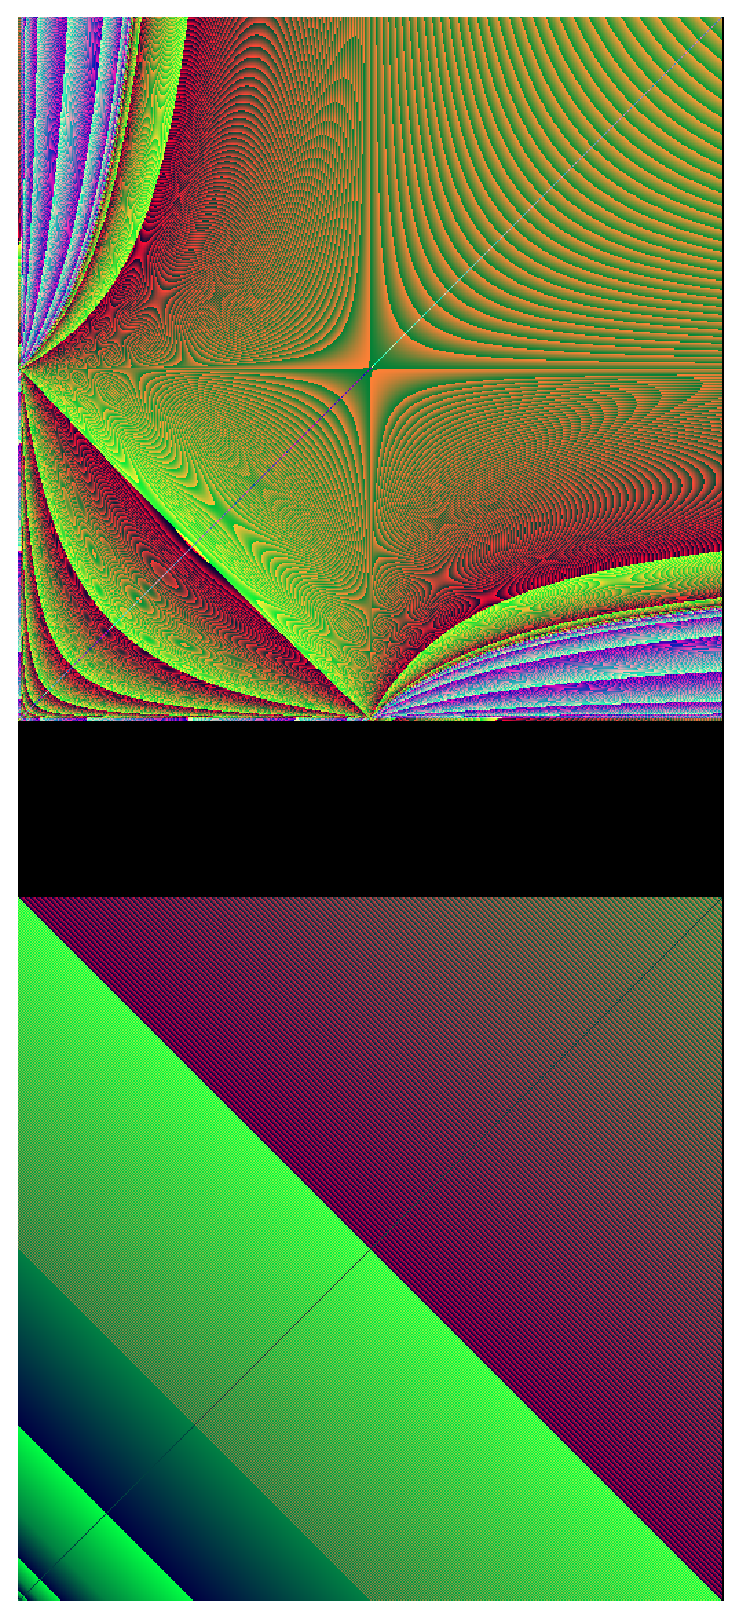
\includegraphics[angle=270,origin=b,width=0.80\textwidth]{inv.eps}
\caption{Inverse matrix}
\end{figure}

This is a 512x512 inverse matrix calculation (LU decomposition). Eight rows are calculated by one burst operation. Mapdist = 0 because it is NOT stencil calculation.

\begin{screen}
\tiny
\begin{verbatim}
  /* LU Decompose */
  for (i=0; i<M+1; i++)
    p[i] = i;
  for (i=0; i<M; i++) {
    pmax = 0.0;
    k = -1;
    for (j=i; j<M; j++) {
      if (pmax < fabsf(A[p[j]*M+i])) {
        pmax = fabsf(A[p[j]*M+i]);
        k = j;
      }
    }
    if (k == -1) {
      fprintf(stderr, "can't solve\n");
      exit(1);
    }
    j = p[k]; p[k] = p[i]; p[i] = j;
    A[p[i]*M+i] = 1.0/A[p[i]*M+i];
    for (j=i+1; j<M; j++) {
      A[p[j]*M+i] *= A[p[i]*M+i];
      for (k=i+1; k<M; k++)
        A[p[j]*M+k] -= A[p[j]*M+i]*A[p[i]*M+k];
    }
  }
\end{verbatim}
\end{screen}

\begin{screen}
\tiny
\begin{verbatim}
  /* LU Decompose */
  for (i=0; i<M+1; i++)
    p[i] = i;
  for (i=0; i<M; i++) { /* Column direction */
    pmax = 0.0;
    k = -1;
    for (j=i; j<M; j++) { /* Search in row direction */
      if (pmax < fabsf(A[p[j]*M+i])) {
        pmax = fabsf(A[p[j]*M+i]);
        k = j;
      }
    }
    if (k == -1) {
      fprintf(stderr, "can't solve\n");
      exit(1);
    }
    j = p[k]; p[k] = p[i]; p[i] = j;
    A[p[i]*M+i] = 1.0/A[p[i]*M+i];
    for (j=i+1; j<M; j++) /* row direction */
      A[p[j]*M+i] *= A[p[i]*M+i];
    for (j=i+1; j<M; j+=NCHIP*H) { /* row direction */
      /********************************************/
      for (CHIP=0; CHIP<NCHIP; CHIP++) {
        for (k=0; k<M-(i+1); k++) { /* Innermost row direction */
          for (h=0; h<H; h++) { /* vertical (parallel) execution */
            if (j+h*NCHIP+CHIP<M) A[p[j+h*NCHIP+CHIP]*M+i+1+k] -= A[p[j+h*NCHIP+CHIP]*M+i]*A[p[i]*M+i+1+k];
                                                     /* Unlike successive inverses, repeat element-wise single subtraction instead of accumurate */
                                                     /* const:A[p[j]][0] * LMM A[p[  0]][*] */
                                                     /*        ��                           */
            /*   v A[p[j]*M+i]         */            /*   LMM A[p[j>0]][*] accumulate (No dependency due to j, j + 1, .., 479 in column direction) */
            /***************************/
            /* + - - - - - - - - - - - */ /* A[p[i]] First row       */ /* The first row can be reused until i update */
            /* | * > > > > > > > > > > */ /* A[p[j]] Subtract from next line */ /* Map one row to LMM */
            /* | v + - - - - - - - - - */
            /* | v | * > > > > > > > > */ /* Repeat j + = 60 until i is updated with accommodating M / 60 */
            /* | v | v + - - - - - - - */ /* Fraction control by line number comparison and cst */
            /* | v | v - + - - - - - - */ /* + CHIP#1 h=0 */
            /* | v | v - - + - - - - - */ /* + CHIP#0 h=1 */
            /* | v | v - - - + - - - - */ /* + CHIP#1 h=1 */
            /* | v | v - - - - + - - - */ /* + CHIP#0 h=2 */
            /* | v | v - - - - - + - - */ /* + CHIP#1 h=2 */
            /* | v | v - - - - - - + - */ /* + CHIP#0 h=3 */
            /* | v | v - - - - - - - + */ /* + CHIP#1 h=3 */
            /***************************/ /* Up to 60 rows can be mapped */
          }
        }
      }
      /********************************************/
    }
  }
\end{verbatim}
\end{screen}

\begin{screen}
\tiny
\begin{verbatim}
  /* LUʬ�� */
  for (i=0; i<M+1; i++)
    p[i] = i;
  for (i=0; i<M; i++) { /* ������ */
    pmax = 0.0;
    k = -1;
    for (j=i; j<M; j++) { /* ��������õ�� */
      if (pmax < fabsf(A[j*M+i])) {
        pmax = fabsf(A[j*M+i]);
        k = j;
      }
    }
    if (k == -1) {
      fprintf(stderr, "can't solve\n");
      exit(1);
    }
    j = p[k]; p[k] = p[i]; p[i] = j;
    for (j=0; j<M; j++) { /* real pivotting */            /*��*/
      tmp = A[k*M+j]; A[k*M+j] = A[i*M+j]; A[i*M+j] = tmp;/*��*/
    }                                                     /*��*/
    A[i*M+i] = 1.0/A[i*M+i];                              /*��*/
    for (j=i+1; j<M; j++) /* ������ */
      A[j*M+i] *= A[i*M+i];

    Uint *top  = &A[i*M+i];
    Uint *topw = (Ull)top;
    Uint  len  = M-i;
    Uint  len2 = len+(RMGRP-1)*M;
    Uint  grp;
    /* FPGA�µ���j-loop�κǽ�(len=1)��ư���ʤ��Τ�,�Ĥ��Ǥ�ARM�Τۤ���®������len��ARM�Ǽ¹� 2019/3/1 Nakashima */
    if (len < 16) { /* len<1�Ǥ�����ʤΤ���ǽ���粽�Ƿ��Ƥ褤 */
      for (j=i+1; j<M; j+=NCHIP*H*RMGRP) { /* ������ */
        for (CHIP=0; CHIP<NCHIP; CHIP++) {
          for (h=0; h<H; h++) { /* vertical (parallel) execution */
            for (grp=0; grp<RMGRP; grp++) {
              for (k=0; k<M-(i+1); k++) { /* ���������� */
                if (j+h*NCHIP*RMGRP+CHIP*RMGRP+grp<M) A[(j+h*NCHIP*RMGRP+CHIP*RMGRP+grp)*M+i+1+k] -= A[(j+h*NCHIP*RMGRP+CHIP*RMGRP+grp)*M+i]*A[i*M+i+1+k];
    } } } } } }
    else {
    for (j=i+1; j<M; j+=NCHIP*H*RMGRP) { /* ������ */
      /********************************************/
      Uint  l00[NCHIP],  l01[NCHIP],  l02[NCHIP],  l03[NCHIP],  l04[NCHIP],  l05[NCHIP],  l06[NCHIP],  l07[NCHIP]; /* j<M-(h*NCHIP+CHIP) */
      Uint  l08[NCHIP],  l09[NCHIP],  l10[NCHIP],  l11[NCHIP],  l12[NCHIP],  l13[NCHIP],  l14[NCHIP],  l15[NCHIP]; /* j<M-(h*NCHIP+CHIP) */
      Uint *d00[NCHIP], *d01[NCHIP], *d02[NCHIP], *d03[NCHIP], *d04[NCHIP], *d05[NCHIP], *d06[NCHIP], *d07[NCHIP]; /* A[p[j+h*NCHIP+CHIP]*M+k] */
      Uint *d08[NCHIP], *d09[NCHIP], *d10[NCHIP], *d11[NCHIP], *d12[NCHIP], *d13[NCHIP], *d14[NCHIP], *d15[NCHIP]; /* A[p[j+h*NCHIP+CHIP]*M+k] */
      Uint *d00w[NCHIP],*d01w[NCHIP],*d02w[NCHIP],*d03w[NCHIP],*d04w[NCHIP],*d05w[NCHIP],*d06w[NCHIP],*d07w[NCHIP];/* A[p[j+h*NCHIP+CHIP]*M+k] */
      Uint *d08w[NCHIP],*d09w[NCHIP],*d10w[NCHIP],*d11w[NCHIP],*d12w[NCHIP],*d13w[NCHIP],*d14w[NCHIP],*d15w[NCHIP];/* A[p[j+h*NCHIP+CHIP]*M+k] */
      for (CHIP=0; CHIP<NCHIP; CHIP++) { /* output channels are parallelized by multi-chip (OC/#chip) */
        l00[CHIP]=(j+ 0*NCHIP*RMGRP+CHIP*RMGRP<M)?(j+ 0*NCHIP*RMGRP+CHIP*RMGRP):M;l01[CHIP]=(j+ 1*NCHIP*RMGRP+CHIP*RMGRP<M)?(j+ 1*NCHIP*RMGRP+CHIP*RMGRP):M;
                :
        l14[CHIP]=(j+14*NCHIP*RMGRP+CHIP*RMGRP<M)?(j+14*NCHIP*RMGRP+CHIP*RMGRP):M;l15[CHIP]=(j+15*NCHIP*RMGRP+CHIP*RMGRP<M)?(j+15*NCHIP*RMGRP+CHIP*RMGRP):M;
        d00[CHIP] = &A[l00[CHIP]*M+i];   d01[CHIP] = &A[l01[CHIP]*M+i];
                :
        d14[CHIP] = &A[l14[CHIP]*M+i];   d15[CHIP] = &A[l15[CHIP]*M+i];
        d00w[CHIP]= (Ull)d00[CHIP];      d01w[CHIP]= (Ull)d01[CHIP];
                :
        d14w[CHIP]= (Ull)d14[CHIP];      d15w[CHIP]= (Ull)d15[CHIP];
      }
//EMAX5A begin inv_x1 mapdist=0
/*3*/ for (CHIP=0; CHIP<NCHIP; CHIP++) {
  /*2*/ for (INIT1=1,LOOP1=RMGRP,rofs=0-M*4; LOOP1--; INIT1=0) {                             /* stage#0 *//* mapped to FOR() on BR[63][1][0] */
    /*1*/ for (INIT0=1,LOOP0=M-(i+1),cofs=0; LOOP0--; INIT0=0) { /* stage#0 *//* mapped to FOR() on BR[63][0][0] */
            exe(OP_ADD, &cofs, INIT0?cofs:cofs, EXP_H3210, 4LL, EXP_H3210, 0LL, EXP_H3210, OP_AND, 0x00000000ffffffffLL, OP_NOP, 0LL); /* stage#0 */
            exe(OP_ADD, &rofs, rofs, EXP_H3210, INIT0?M*4:0, EXP_H3210, 0LL, EXP_H3210, OP_NOP, 0LL, OP_NOP, 0LL);                     /* stage#0 */
            exe(OP_ADD, &oofs, rofs, EXP_H3210, cofs, EXP_H3210, 0LL, EXP_H3210, OP_AND, 0x00000000ffffffffLL, OP_NOP, 0LL);           /* stage#1 */
            exe(OP_CMP_LT,   &cc0,         l00[CHIP],   EXP_H3210, M,         EXP_H3210, 0LL,         EXP_H3210, OP_NOP, 0LL, OP_NOP, 0LL); /* stage#1              LD
            mop(OP_LDWR,  1, &BR[2][2][1], top,         cofs, MSK_W0, topw,       len, 0, 0, NULL, len);  /* A[p[i]*M+k]                       stage#2              |
            mop(OP_LDWR,  1, &BR[2][0][1], d00[CHIP],   oofs, MSK_W0, d00w[CHIP], len2,0, 1, NULL, len2); /* A[p[j+h*NCHIP+CHIP]*M+k]          stage#2  +->         |
            mop(OP_LDWR,  1, &BR[2][1][1], d00[CHIP],   rofs, MSK_W0, d00w[CHIP], len2,0, 1, NULL, len2); /* A[p[j+h*NCHIP+CHIP]*M+k]          stage#2  +->         |
            exe(OP_FMS,      &AR[2][0],    BR[2][0][1], EXP_H3210, BR[2][1][1], EXP_H3210, BR[2][2][1], EXP_H3210, OP_NOP, 0LL, OP_NOP, 0); /* stage#2  |   ������  |
            cex(OP_CEXE,     &ex0,   0, 0, 0, cc0, 0xaaaa);                                                                                 /* stage#2  |  AR[1]    |
            mop(OP_STWR,ex0, &AR[2][0],    oofs,   d00[CHIP], MSK_D0, d00w[CHIP], len2, 0, 1, NULL, len2);                                  /* stage#2  |    + ST   v
#if (H>1)                                                                                                                                   /*          *--------- BR[2]
            exe(OP_CMP_LT,   &cc0,         l01[CHIP],   EXP_H3210, M,         EXP_H3210, 0LL,         EXP_H3210, OP_NOP, 0LL, OP_NOP, 0LL); /* stage#2              LD
            mop(OP_LDWR,  1, &BR[3][2][1], top,         cofs, MSK_W0, topw,       len, 0, 0, NULL, len);  /* A[p[i]*M+k]                       stage#3              |
            mop(OP_LDWR,  1, &BR[3][0][1], d01[CHIP],   oofs, MSK_W0, d01w[CHIP], len2,0, 1, NULL, len2); /* A[p[j+h*NCHIP+CHIP]*M+k]          stage#3  +->         |
            mop(OP_LDWR,  1, &BR[3][1][1], d01[CHIP],   rofs, MSK_W0, d01w[CHIP], len2,0, 1, NULL, len2); /* A[p[j+h*NCHIP+CHIP]*M+k]          stage#3  +->         |
            exe(OP_FMS,      &AR[3][0],    BR[3][0][1], EXP_H3210, BR[3][1][1], EXP_H3210, BR[3][2][1], EXP_H3210, OP_NOP, 0LL, OP_NOP, 0); /* stage#3  |   ������  |
            cex(OP_CEXE,     &ex0,   0, 0, 0, cc0, 0xaaaa);                                                                                 /* stage#3  |  AR[2]    |
            mop(OP_STWR,ex0, &AR[3][0],    oofs,   d01[CHIP], MSK_D0, d01w[CHIP], len2, 0, 1, NULL, len2);                                  /* stage#3  |    + ST   v
                :
#if (H>12)                                                                                                                                  /*          *--------- BR[13]
            exe(OP_CMP_LT,   &cc0,         l12[CHIP],   EXP_H3210, M,         EXP_H3210, 0LL,         EXP_H3210, OP_NOP, 0LL, OP_NOP, 0LL); /* stage#13             LD
            mop(OP_LDWR,  1, &BR[14][2][1],top,         cofs, MSK_W0, topw,       len, 0, 0, NULL, len);  /* A[p[i]*M+k] stage#1               stage#14             |
            mop(OP_LDWR,  1, &BR[14][0][1],d12[CHIP],   oofs, MSK_W0, d12w[CHIP], len2,0, 1, NULL, len2); /* A[p[j+h*NCHIP+CHIP]*M+k]          stage#14 +->         |
            mop(OP_LDWR,  1, &BR[14][1][1],d12[CHIP],   rofs, MSK_W0, d12w[CHIP], len2,0, 1, NULL, len2); /* A[p[j+h*NCHIP+CHIP]*M+k]          stage#14 +->         |
            exe(OP_FMS,      &AR[14][0],   BR[14][0][1],EXP_H3210, BR[14][1][1], EXP_H3210, BR[14][2][1],EXP_H3210, OP_NOP, 0LL, OP_NOP, 0);/* stage#14 |   ������  |
            cex(OP_CEXE,     &ex0,   0, 0, 0, cc0, 0xaaaa);                                                                                 /* stage#14 |  AR[13]   |
            mop(OP_STWR,ex0, &AR[14][0],   oofs,   d12[CHIP], MSK_D0, d12w[CHIP], len2, 0, 1, NULL, len2);                                  /* stage#14 |    + ST   v
#if (H>13)                                                                                                                                  /*          *--------- BR[14]
            exe(OP_CMP_LT,   &cc0,         l13[CHIP],   EXP_H3210, M,         EXP_H3210, 0LL,         EXP_H3210, OP_NOP, 0LL, OP_NOP, 0LL); /* stage#14             LD
            mop(OP_LDWR,  1, &BR[15][2][1],top,         cofs, MSK_W0, topw,       len, 0, 0, NULL, len);  /* A[p[i]*M+k] stage#1               stage#15             |
            mop(OP_LDWR,  1, &BR[15][0][1],d13[CHIP],   oofs, MSK_W0, d13w[CHIP], len2,0, 1, NULL, len2); /* A[p[j+h*NCHIP+CHIP]*M+k]          stage#15 +->         |
            mop(OP_LDWR,  1, &BR[15][1][1],d13[CHIP],   rofs, MSK_W0, d13w[CHIP], len2,0, 1, NULL, len2); /* A[p[j+h*NCHIP+CHIP]*M+k]          stage#15 +->         |
            exe(OP_FMS,      &AR[15][0],   BR[15][0][1],EXP_H3210, BR[15][1][1], EXP_H3210, BR[15][2][1],EXP_H3210, OP_NOP, 0LL, OP_NOP, 0);/* stage#15 |   ������  |
            cex(OP_CEXE,     &ex0,   0, 0, 0, cc0, 0xaaaa);                                                                                 /* stage#15 |  AR[14]   |
            mop(OP_STWR,ex0, &AR[15][0],   oofs,   d13[CHIP], MSK_D0, d13w[CHIP], len2, 0, 1, NULL, len2);                                  /* stage#15 |    + ST   v
#if (H>14)                                                                                                                                  /*          *--------- BR[15]
            exe(OP_CMP_LT,   &cc0,         l14[CHIP],   EXP_H3210, M,         EXP_H3210, 0LL,         EXP_H3210, OP_NOP, 0LL, OP_NOP, 0LL); /* stage#15             LD
            mop(OP_LDWR,  1, &BR[16][2][1],top,         cofs, MSK_W0, topw,       len, 0, 0, NULL, len);  /* A[p[i]*M+k] stage#1               stage#16             |
            mop(OP_LDWR,  1, &BR[16][0][1],d14[CHIP],   oofs, MSK_W0, d14w[CHIP], len2,0, 1, NULL, len2); /* A[p[j+h*NCHIP+CHIP]*M+k]          stage#16 +->         |
            mop(OP_LDWR,  1, &BR[16][1][1],d14[CHIP],   rofs, MSK_W0, d14w[CHIP], len2,0, 1, NULL, len2); /* A[p[j+h*NCHIP+CHIP]*M+k]          stage#16 +->         |
            exe(OP_FMS,      &AR[16][0],   BR[16][0][1],EXP_H3210, BR[16][1][1], EXP_H3210, BR[16][2][1],EXP_H3210, OP_NOP, 0LL, OP_NOP, 0);/* stage#16 |   ������  |
            cex(OP_CEXE,     &ex0,   0, 0, 0, cc0, 0xaaaa);                                                                                 /* stage#16 |  AR[15]   |
            mop(OP_STWR,ex0, &AR[16][0],   oofs,   d14[CHIP], MSK_D0, d14w[CHIP], len2, 0, 1, NULL, len2);                                  /* stage#16 |    + ST   v
#if (H>15)                                                                                                                                  /*          *--------- BR[16]
            exe(OP_CMP_LT,   &cc0,         l15[CHIP],   EXP_H3210, M,         EXP_H3210, 0LL,         EXP_H3210, OP_NOP, 0LL, OP_NOP, 0LL); /* stage#16             LD
            mop(OP_LDWR,  1, &BR[17][2][1],top,         cofs, MSK_W0, topw,       len, 0, 0, NULL, len);  /* A[p[i]*M+k] stage#1               stage#17             |
            mop(OP_LDWR,  1, &BR[17][0][1],d15[CHIP],   oofs, MSK_W0, d15w[CHIP], len2,0, 1, NULL, len2); /* A[p[j+h*NCHIP+CHIP]*M+k]          stage#17 +->         |
            mop(OP_LDWR,  1, &BR[17][1][1],d15[CHIP],   rofs, MSK_W0, d15w[CHIP], len2,0, 1, NULL, len2); /* A[p[j+h*NCHIP+CHIP]*M+k]          stage#17 +->         |
            exe(OP_FMS,      &AR[17][0],   BR[17][0][1],EXP_H3210, BR[17][1][1], EXP_H3210, BR[17][2][1],EXP_H3210, OP_NOP, 0LL, OP_NOP, 0);/* stage#17 |   ������  |
            cex(OP_CEXE,     &ex0,   0, 0, 0, cc0, 0xaaaa);                                                                                 /* stage#17 |  AR[16]   |
            mop(OP_STWR,ex0, &AR[17][0],   oofs,   d15[CHIP], MSK_D0, d15w[CHIP], len2, 0, 1, NULL, len2);                                  /* stage#17 |    + ST   v
                                                                                                                                            /*          *--------- BR[17]
#endif
      } } }
//EMAX5A end
      /********************************************/
    } /* j-loop */
//EMAX5A drain_dirty_lmm
\end{verbatim}
\end{screen}

\begin{figure}[htbp]
\center
\epsfile{file=inv+rmm-inv_x1-emax6.eps,width=1.00\textwidth}
\caption{�չ���(1/3)}
\end{figure}

\clearpage

\subsection{Inverse matrix (2/3)}

Here is a 512x512 inverse matrix calculation (forward elimination). Eight rows are calculated by one burst operation. Mapdist = 0 because it is NOT stencil calculation.

\begin{screen}
\tiny
\begin{verbatim}
  /* �չ�����Ⱦ */
  for (i=0; i<M; i++) {
    for (j=0; j<M; j++)
      b[p[j]] = (i==j)?1.0:0.0;
    /*for (j=1; j<M; j++) { *//*�̾��ϢΩ����������ξ��*/
    for (j=i+1; j<M; j++) { /* �չ���(b[]=E)�ξ��,k<i�Ǥ�b[]==0�ʤΤ�j=i+1���鳫�� */
      /*for (k=0; k<j; k++) *//*�̾��ϢΩ����������ξ��*/
      for (k=i; k<j; k++) /* �չ���(b[]=E)�ξ��,k<i�Ǥ�b[]==0�ʤΤ�k=i���鳫�� */
        b[p[j]] -= A[p[j]*M+k]*b[p[k]];
    }
  }
\end{verbatim}
\end{screen}

\begin{screen}
\tiny
\begin{verbatim}
  /* �չ������ */
  for (i=0; i<M; i++) { /* ������ */
    for (j=0; j<M; j++) /* ������ */
      b[i*M+j] = (i==j)?1.0:0.0;
  }
  for (i=0; i<M; i+=NCHIP*H) { /* ������ */
    for (j=1; j<M; j++) { /* ������ */
      /********************************************/
      for (CHIP=0; CHIP<NCHIP; CHIP++) {
        for (k=0; k<j; k++) { /* ���������� */
          for (h=0; h<H; h++) { /* vertical (parallel) execution */
            b[(i+CHIP*H+h)*M+j] -= A[p[j]*M+k]*b[(i+CHIP*H+h)*M+k];
                                        /* b[*]��Ĥ����֤�����,A�������. j�����������б����뤬�������ΰ�ư��k��Ĺ���ʤ� */
                                        /* ����Ĺk��H������Ÿ����������Τ��񤷤�.k��read-modify-write�β�ž���˼������뤷���ʤ� */
                                        /* b[*]��A[j][*]��Ʊ��LMM���������� ����64KB/4/2=��8K����,b[*]�򤤤���ư�����ʤ��� */
                                        /* ��ž��j�����Ŭ�Ѥ���ˤ�,i��WxH������Ÿ������Τ����� */
              /*           ����A[p[j]][*]��broadcast��ǽ ��A[p[j]][*]��p[j]����Ϣ³�ʤΤ�1K���ǤޤǼ���.�Ĥޤ���ť롼��Ÿ����̵�� */
              /* +-----------------------------------+     +------+ +------+ +------+ */
              /* b[ 3][j]-=A[p[j]][0:j-1] b[ 3][0:j-1]     b[ 2][*] b[ 1][*] b[ 0][*] */
              /*                                                                      */
              /* b[ 7][j]-=A[p[j]][0:j-1] b[ 7][0:j-1]     b[ 6][*] b[ 5][*] b[ 4][*] */
              /* b[59][j]-=A[p[j]][0:j-1] b[59][0:j-1]     b[58][*] b[57][*] b[56][*] */
          }
        }
      }
      /********************************************/
    }
  }
\end{verbatim}
\end{screen}

\begin{screen}
\tiny
\begin{verbatim}
  /* �չ�����Ⱦ */
  for (i=0; i<M; i++) { /* ������ */
    for (j=0; j<M; j++) /* ������ */
      b[i*M+j] = (i==j)?1.0:0.0;
  }
  for (i=0; i<M; i+=NCHIP*H) { /* ������ */
    /*for (j=1; j<M; j++) { *//*�̾��ϢΩ����������ξ��*/
    for (j=i+1; j<M; j++) { /* �չ���(b[]=E)�ξ��,k<i�Ǥ�b[]==0�ʤΤ�j=i+1���鳫�� */
      Uint *top  = &A[p[j]*M+i];                                     /* A[p[j]*M+k] */
      Uint *topw = (Ull)top;
      /*Uint  len = (j+1)/2;*/
      Uint  len = j-i;/* b��ñ�̹���ξ��,k<i�Ǥ�b[]==0�ʤΤ�k=i���鳫�� */
      /********************************************/
      if (len < 2) { /* len<1�Ǥ�����ʤΤ���ǽ���粽�Ƿ��Ƥ褤 */
        for (CHIP=0; CHIP<NCHIP; CHIP++) {
        /*for (k=0; k<j; k++) { *//*�̾��ϢΩ����������ξ��*/
          for (k=i; k<j; k++) { /* �չ���(b[]=E)�ξ��,k<i�Ǥ�b[]==0�ʤΤ�k=i���鳫�� */
            for (h=0; h<H; h++) { /* vertical (parallel) execution */
              b[(i+CHIP*H+h)*M+j] -= A[p[j]*M+k]*b[(i+CHIP*H+h)*M+k];
            }
          }
        }
      }
      else {
      Uint  jc = j-i;
      Ull   Ajk; /* k=0...j-1 */
      Ull   b000, b001;
      Uint  l000[NCHIP],  l010[NCHIP],  l020[NCHIP],  l030[NCHIP],  l040[NCHIP],  l050[NCHIP],  l060[NCHIP],  l070[NCHIP];  /* (i+CHIP*W*H+h*W+w)        */
      Uint  l080[NCHIP],  l090[NCHIP],  l100[NCHIP],  l110[NCHIP],  l120[NCHIP],  l130[NCHIP],  l140[NCHIP],  l150[NCHIP];  /* (i+CHIP*W*H+h*W+w)        */
      Uint *t000[NCHIP], *t010[NCHIP], *t020[NCHIP], *t030[NCHIP], *t040[NCHIP], *t050[NCHIP], *t060[NCHIP], *t070[NCHIP];  /* b[(i+CHIP*W*H+h*W+w)*M+k] */
      Uint *t080[NCHIP], *t090[NCHIP], *t100[NCHIP], *t110[NCHIP], *t120[NCHIP], *t130[NCHIP], *t140[NCHIP], *t150[NCHIP];  /* b[(i+CHIP*W*H+h*W+w)*M+k] */
      Uint *t000w[NCHIP],*t010w[NCHIP],*t020w[NCHIP],*t030w[NCHIP],*t040w[NCHIP],*t050w[NCHIP],*t060w[NCHIP],*t070w[NCHIP]; /* b[(i+CHIP*W*H+h*W+w)*M+k] */
      Uint *t080w[NCHIP],*t090w[NCHIP],*t100w[NCHIP],*t110w[NCHIP],*t120w[NCHIP],*t130w[NCHIP],*t140w[NCHIP],*t150w[NCHIP]; /* b[(i+CHIP*W*H+h*W+w)*M+k] */
      Uint *d000[NCHIP], *d010[NCHIP], *d020[NCHIP], *d030[NCHIP], *d040[NCHIP], *d050[NCHIP], *d060[NCHIP], *d070[NCHIP];  /* b[(i+CHIP*W*H+h*W+w)*M+j] */
      Uint *d080[NCHIP], *d090[NCHIP], *d100[NCHIP], *d110[NCHIP], *d120[NCHIP], *d130[NCHIP], *d140[NCHIP], *d150[NCHIP];  /* b[(i+CHIP*W*H+h*W+w)*M+j] */
      Uint *d000w[NCHIP],*d010w[NCHIP],*d020w[NCHIP],*d030w[NCHIP],*d040w[NCHIP],*d050w[NCHIP],*d060w[NCHIP],*d070w[NCHIP]; /* b[(i+CHIP*W*H+h*W+w)*M+j] */
      Uint *d080w[NCHIP],*d090w[NCHIP],*d100w[NCHIP],*d110w[NCHIP],*d120w[NCHIP],*d130w[NCHIP],*d140w[NCHIP],*d150w[NCHIP]; /* b[(i+CHIP*W*H+h*W+w)*M+j] */
      for (CHIP=0; CHIP<NCHIP; CHIP++) { /* output channels are parallelized by multi-chip (OC/#chip) */
        l000[CHIP] = (i+CHIP*H+ 0+0)*M;         l010[CHIP] = (i+CHIP*H+ 1+0)*M;         l020[CHIP] = (i+CHIP*H+ 2+0)*M;         l030[CHIP] = (i+CHIP*H+ 3+0)*M;
              :
        l120[CHIP] = (i+CHIP*H+12+0)*M;         l130[CHIP] = (i+CHIP*H+13+0)*M;         l140[CHIP] = (i+CHIP*H+14+0)*M;         l150[CHIP] = (i+CHIP*H+15+0)*M;
        t000[CHIP] = &b[l000[CHIP]+i]; t010[CHIP] = &b[l010[CHIP]+i];
              :
        t140[CHIP] = &b[l140[CHIP]+i]; t150[CHIP] = &b[l150[CHIP]+i];
        t000w[CHIP]= (Ull)t000[CHIP];  t010w[CHIP]= (Ull)t010[CHIP];
              :
        t140w[CHIP]= (Ull)t140[CHIP];  t150w[CHIP]= (Ull)t150[CHIP];
        d000[CHIP] = &b[l000[CHIP]+j]; d010[CHIP] = &b[l010[CHIP]+j];
              :
        d140[CHIP] = &b[l140[CHIP]+j]; d150[CHIP] = &b[l150[CHIP]+j];
        d000w[CHIP]= (Ull)d000[CHIP];  d010w[CHIP]= (Ull)d010[CHIP];
              :
        d140w[CHIP]= (Ull)d140[CHIP];  d150w[CHIP]= (Ull)d150[CHIP];
      }
//EMAX5A begin inv_x2 mapdist=0
/*2*/ for (CHIP=0; CHIP<NCHIP; CHIP++) {
  /*1*/ for (INIT0=1,LOOP0=jc,cofs=0-4; LOOP0--; INIT0=0) { /* stage#0 *//* mapped to FOR() on BR[63][0][0] */
          exe(OP_ADD, &cofs, cofs, EXP_H3210, 4LL, EXP_H3210, 0LL, EXP_H3210, OP_AND, 0x00000000ffffffffLL, OP_NOP, 0LL); /* stage#0 */
          mop(OP_LDWR,  1, &Ajk,         top,          cofs, MSK_W0, topw,        len, 0, 0, NULL, len);  /* A[p[j]*M+k]              */
          mop(OP_LDWR,  1, &BR[1][3][1], t000[CHIP],   cofs, MSK_W0, t000w[CHIP], len, 0, 1, NULL, len);  /* b[(i+CHIP*W*H+h*W+0)*M+k]*//* stage#1.3 +->xxx     LD */
          mop(OP_LDWR,  1, &b000,        d000[CHIP],   0,    MSK_W0, d000w[CHIP], 1,   0, 1, NULL, 1);    /* b[(i+CHIP*W*H+h*W+0)*M+j]*//* stage#2.0 |   ������ |  */
          exe(OP_FMS,      &b000,        b000,         EXP_H3210, Ajk, EXP_H3210, BR[1][3][1], EXP_H3210, OP_NOP, 0LL, OP_NOP, 0LL);    /* stage#2.0 +- xxx+ST  v  */
          mop(OP_STWR,  1, &b000,        0,      d000[CHIP], MSK_D0, d000w[CHIP], 1,   0, 1, NULL, 1);                                  /* stage#2.0 +-------- xxx */
#if (H>1)
          mop(OP_LDWR,  1, &BR[2][3][1], t010[CHIP],   cofs, MSK_W0, t010w[CHIP], len, 0, 1, NULL, len);  /* b[(i+CHIP*W*H+h*W+1)*M+k]*//* stage#2.3 +->xxx     LD */
          mop(OP_LDWR,  1, &b000,        d010[CHIP],   0,    MSK_W0, d010w[CHIP], 1,   0, 1, NULL, 1);    /* b[(i+CHIP*W*H+h*W+0)*M+j]*//* stage#3.0 |   ������ |  */
          exe(OP_FMS,      &b000,        b000,         EXP_H3210, Ajk, EXP_H3210, BR[2][3][1], EXP_H3210, OP_NOP, 0LL, OP_NOP, 0LL);    /* stage#3.0 +- xxx+ST  v  */
          mop(OP_STWR,  1, &b000,        0,      d010[CHIP], MSK_D0, d010w[CHIP], 1,   0, 1, NULL, 1);                                  /* stage#3.0 +-------- xxx */
                :
#if (H>8)
          mop(OP_LDWR,  1, &BR[9][3][1], t080[CHIP],   cofs, MSK_W0, t080w[CHIP], len, 0, 1, NULL, len);  /* b[(i+CHIP*W*H+h*W+0)*M+k]*//* stage#9.3 +->xxx     LD */
          mop(OP_LDWR,  1, &b000,        d080[CHIP],   0,    MSK_W0, d080w[CHIP], 1,   0, 1, NULL, 1);    /* b[(i+CHIP*W*H+h*W+0)*M+j]*//* stage#10.0|   ������ |  */
          exe(OP_FMS,      &b000,        b000,         EXP_H3210, Ajk, EXP_H3210, BR[9][3][1], EXP_H3210, OP_NOP, 0LL, OP_NOP, 0LL);    /* stage#10.0+- xxx+ST  v  */
          mop(OP_STWR,  1, &b000,        0,      d080[CHIP], MSK_D0, d080w[CHIP], 1,   0, 1, NULL, 1);                                  /* stage#10.0+-------- xxx */
#if (H>9)
          mop(OP_LDWR,  1, &BR[10][3][1],t090[CHIP],   cofs, MSK_W0, t090w[CHIP], len, 0, 1, NULL, len);  /* b[(i+CHIP*W*H+h*W+0)*M+k]*//* stage#10.3+->xxx     LD */
          mop(OP_LDWR,  1, &b000,        d090[CHIP],   0,    MSK_W0, d090w[CHIP], 1,   0, 1, NULL, 1);    /* b[(i+CHIP*W*H+h*W+0)*M+j]*//* stage#11.0|   ������ |  */
          exe(OP_FMS,      &b000,        b000,         EXP_H3210, Ajk, EXP_H3210, BR[10][3][1],EXP_H3210, OP_NOP, 0LL, OP_NOP, 0LL);    /* stage#11.0+- xxx+ST  v  */
          mop(OP_STWR,  1, &b000,        0,      d090[CHIP], MSK_D0, d090w[CHIP], 1,   0, 1, NULL, 1);                                  /* stage#11.0+-------- xxx */
#if (H>10)
          mop(OP_LDWR,  1, &BR[11][3][1],t100[CHIP],   cofs, MSK_W0, t100w[CHIP], len, 0, 1, NULL, len);  /* b[(i+CHIP*W*H+h*W+0)*M+k]*//* stage#11.3+->xxx     LD */
          mop(OP_LDWR,  1, &b000,        d100[CHIP],   0,    MSK_W0, d100w[CHIP], 1,   0, 1, NULL, 1);    /* b[(i+CHIP*W*H+h*W+0)*M+j]*//* stage#12.0|   ������ |  */
          exe(OP_FMS,      &b000,        b000,         EXP_H3210, Ajk, EXP_H3210, BR[11][3][1],EXP_H3210, OP_NOP, 0LL, OP_NOP, 0LL);    /* stage#12.0+- xxx+ST  v  */
          mop(OP_STWR,  1, &b000,        0,      d100[CHIP], MSK_D0, d100w[CHIP], 1,   0, 1, NULL, 1);                                  /* stage#12.0+-------- xxx */
#if (H>11)
          mop(OP_LDWR,  1, &BR[12][3][1],t110[CHIP],   cofs, MSK_W0, t110w[CHIP], len, 0, 1, NULL, len);  /* b[(i+CHIP*W*H+h*W+0)*M+k]*//* stage#12.3+->xxx     LD */
          mop(OP_LDWR,  1, &b000,        d110[CHIP],   0,    MSK_W0, d110w[CHIP], 1,   0, 1, NULL, 1);    /* b[(i+CHIP*W*H+h*W+0)*M+j]*//* stage#13.0|   ������ |  */
          exe(OP_FMS,      &b000,        b000,         EXP_H3210, Ajk, EXP_H3210, BR[12][3][1],EXP_H3210, OP_NOP, 0LL, OP_NOP, 0LL);    /* stage#13.0+- xxx+ST  v  */
          mop(OP_STWR,  1, &b000,        0,      d110[CHIP], MSK_D0, d110w[CHIP], 1,   0, 1, NULL, 1);                                  /* stage#13.0+-------- xxx */
#if (H>12)
          mop(OP_LDWR,  1, &BR[13][3][1],t120[CHIP],   cofs, MSK_W0, t120w[CHIP], len, 0, 1, NULL, len);  /* b[(i+CHIP*W*H+h*W+0)*M+k]*//* stage#13.3+->xxx     LD */
          mop(OP_LDWR,  1, &b000,        d120[CHIP],   0,    MSK_W0, d120w[CHIP], 1,   0, 1, NULL, 1);    /* b[(i+CHIP*W*H+h*W+0)*M+j]*//* stage#14.0|   ������ |  */
          exe(OP_FMS,      &b000,        b000,         EXP_H3210, Ajk, EXP_H3210, BR[13][3][1],EXP_H3210, OP_NOP, 0LL, OP_NOP, 0LL);    /* stage#14.0+- xxx+ST  v  */
          mop(OP_STWR,  1, &b000,        0,      d120[CHIP], MSK_D0, d120w[CHIP], 1,   0, 1, NULL, 1);                                  /* stage#14.0+-------- xxx */
#if (H>13)
          mop(OP_LDWR,  1, &BR[14][3][1],t130[CHIP],   cofs, MSK_W0, t130w[CHIP], len, 0, 1, NULL, len);  /* b[(i+CHIP*W*H+h*W+0)*M+k]*//* stage#14.3+->xxx     LD */
          mop(OP_LDWR,  1, &b000,        d130[CHIP],   0,    MSK_W0, d130w[CHIP], 1,   0, 1, NULL, 1);    /* b[(i+CHIP*W*H+h*W+0)*M+j]*//* stage#15.0|   ������ |  */
          exe(OP_FMS,      &b000,        b000,         EXP_H3210, Ajk, EXP_H3210, BR[14][3][1],EXP_H3210, OP_NOP, 0LL, OP_NOP, 0LL);    /* stage#15.0+- xxx+ST  v  */
          mop(OP_STWR,  1, &b000,        0,      d130[CHIP], MSK_D0, d130w[CHIP], 1,   0, 1, NULL, 1);                                  /* stage#15.0+-------- xxx */
#if (H>14)
          mop(OP_LDWR,  1, &BR[15][3][1],t140[CHIP],   cofs, MSK_W0, t140w[CHIP], len, 0, 1, NULL, len);  /* b[(i+CHIP*W*H+h*W+0)*M+k]*//* stage#15.3+->xxx     LD */
          mop(OP_LDWR,  1, &b000,        d140[CHIP],   0,    MSK_W0, d140w[CHIP], 1,   0, 1, NULL, 1);    /* b[(i+CHIP*W*H+h*W+0)*M+j]*//* stage#16.0|   ������ |  */
          exe(OP_FMS,      &b000,        b000,         EXP_H3210, Ajk, EXP_H3210, BR[15][3][1],EXP_H3210, OP_NOP, 0LL, OP_NOP, 0LL);    /* stage#16.0+- xxx+ST  v  */
          mop(OP_STWR,  1, &b000,        0,      d140[CHIP], MSK_D0, d140w[CHIP], 1,   0, 1, NULL, 1);                                  /* stage#16.0+-------- xxx */
#if (H>15)
          mop(OP_LDWR,  1, &BR[16][3][1],t150[CHIP],   cofs, MSK_W0, t150w[CHIP], len, 0, 1, NULL, len);  /* b[(i+CHIP*W*H+h*W+0)*M+k]*//* stage#16.3+->xxx     LD */
          mop(OP_LDWR,  1, &b000,        d150[CHIP],   0,    MSK_W0, d150w[CHIP], 1,   0, 1, NULL, 1);    /* b[(i+CHIP*W*H+h*W+0)*M+j]*//* stage#17.0|   ������ |  */
          exe(OP_FMS,      &b000,        b000,         EXP_H3210, Ajk, EXP_H3210, BR[16][3][1],EXP_H3210, OP_NOP, 0LL, OP_NOP, 0LL);    /* stage#17.0+- xxx+ST  v  */
          mop(OP_STWR,  1, &b000,        0,      d150[CHIP], MSK_D0, d150w[CHIP], 1,   0, 1, NULL, 1);                                  /* stage#17.0+-------- xxx */
#endif
        }
      }
//EMAX5A end
//EMAX5A drain_dirty_lmm
      } /* else */
      /********************************************/
    } /* j-loop */
  }
\end{verbatim}
\end{screen}

\begin{figure}[htbp]
\center
\epsfile{file=inv+rmm-inv_x2-emax6.eps,width=1.00\textwidth}
\caption{�չ���(2/3)}
\end{figure}

\clearpage

\subsection{Inverse Matrix (3/3)}

This is a 512x512 inverse matrix calculation (backward substitution). Eight rows are calculated by one burst operation. Mapdist = 0 because it is NOT stencil calculation.

\begin{screen}
\tiny
\begin{verbatim}
  /* �չ����Ⱦ */
  for (i=0; i<M; i++) {
    for (j=M-1; j>=0; j--) {
      for (k=M-1; k>j; k--)
        b[p[j]] -= A[p[j]*M+k]*x[k];
      inv0[j*M+p[i]] = x[j] = b[p[j]]*A[p[j]*M+j];
    }
  }
\end{verbatim}
\end{screen}

\begin{screen}
\tiny
\begin{verbatim}
  for (i=0; i<M; i+=NCHIP*H) { /* ������ */
    for (j=M-1; j>=0; j--) { /* ������ */
      /********************************************/
      for (CHIP=0; CHIP<NCHIP; CHIP++) {
        for (k=M-1; k>j; k--) { /* ���������� */
          for (h=0; h<H; h++) { /* vertical (parallel) execution */
            b[(i+CHIP*H+h)*M+j] -= A[p[j]*M+k]*x[(i+CHIP*H+h)*M+k];
                                            /* x[*]��A[j][*]��Ʊ��LMM���������� ����64KB/4/2=��8K����,x[*]�򤤤���ư�����ʤ��� */
                                            /* ��ž��j�����Ŭ�Ѥ���ˤ�,i��WxH������Ÿ������Τ����� */
            /*           ����A[p[j]][*]��broadcast��ǽ ��A[p[j]][*]��p[j]����Ϣ³�ʤΤ�1K���ǤޤǼ���.�Ĥޤ���ť롼��Ÿ����̵�� */
            /* +-----------------------------------+     +------+ +------+ +------+ */
            /* b[ 3][j]-=A[p[j]][M-1:j+1] x[ 3][M-1:j+1] b[ 2][*] b[ 1][*] b[ 0][*] */
            /*                                                                      */
            /* b[ 7][j]-=A[p[j]][M-1:j+1] x[ 7][M-1:j+1] b[ 6][*] b[ 5][*] b[ 4][*] */
            /* b[59][j]-=A[p[j]][M-1:j+1] x[59][M-1:j+1] b[58][*] b[57][*] b[56][*] */
          }
        }
      }
      /********************************************/
      for (CHIP=0; CHIP<NCHIP; CHIP++) {
        for (h=0; h<H; h++) { /* vertical (parallel) execution */
          inv1[j*M+p[i+CHIP*H+h+w]] = x[(i+CHIP*H+h)*M+j] = A[p[j]*M+j]*b[(i+CHIP*H+h)*M+j]; /* PIO�ˤ�LMM��x[i*M+j]��ľ�ܹ��� */
                                                                                             /* i�Ϥ��Τޤޤ�,j�����ؤ� */
        }
      }
    }
  }
\end{verbatim}
\end{screen}

\begin{screen}
\tiny
\begin{verbatim}
  /* �չ����Ⱦ */
  for (i=0; i<M; i+=NCHIP*H) { /* ������ */
    for (j=M-1; j>=0; j--) { /* ������ */
      if (j<M-1) {
        Uint *top  = &A[p[j]*M+j+1];                                  /* A[p[j]*M+k] */
        Uint *topw = (Ull)top;
        Uint  len = M-j-1;
        /********************************************/
        if (len < 2) { /* len<1�Ǥ�����ʤΤ���ǽ���粽�Ƿ��Ƥ褤 */
          for (CHIP=0; CHIP<NCHIP; CHIP++) {
            for (k=M-1; k>j; k--) { /* ���������� */
              for (h=0; h<H; h++) { /* vertical (parallel) execution */
                b[(i+CHIP*H+h)*M+j] -= A[p[j]*M+k]*x[(i+CHIP*H+h)*M+k];
              }
            }
          }
        }
        else {
        Uint  jc = M-j-1;
        Ull   Ajk; /* k=j+1...M-1 */
        Ull   b000, b001;
        Uint  l000[NCHIP],  l010[NCHIP],  l020[NCHIP],  l030[NCHIP],  l040[NCHIP],  l050[NCHIP],  l060[NCHIP],  l070[NCHIP];  /* (i+CHIP*W*H+h*W+w)        */
        Uint  l080[NCHIP],  l090[NCHIP],  l100[NCHIP],  l110[NCHIP],  l120[NCHIP],  l130[NCHIP],  l140[NCHIP],  l150[NCHIP];  /* (i+CHIP*W*H+h*W+w)        */
        Uint *t000[NCHIP], *t010[NCHIP], *t020[NCHIP], *t030[NCHIP], *t040[NCHIP], *t050[NCHIP], *t060[NCHIP], *t070[NCHIP];  /* b[(i+CHIP*W*H+h*W+w)*M+k] */
        Uint *t080[NCHIP], *t090[NCHIP], *t100[NCHIP], *t110[NCHIP], *t120[NCHIP], *t130[NCHIP], *t140[NCHIP], *t150[NCHIP];  /* b[(i+CHIP*W*H+h*W+w)*M+k] */
        Uint *t000w[NCHIP],*t010w[NCHIP],*t020w[NCHIP],*t030w[NCHIP],*t040w[NCHIP],*t050w[NCHIP],*t060w[NCHIP],*t070w[NCHIP]; /* b[(i+CHIP*W*H+h*W+w)*M+k] */
        Uint *t080w[NCHIP],*t090w[NCHIP],*t100w[NCHIP],*t110w[NCHIP],*t120w[NCHIP],*t130w[NCHIP],*t140w[NCHIP],*t150w[NCHIP]; /* b[(i+CHIP*W*H+h*W+w)*M+k] */
        Uint *d000[NCHIP], *d010[NCHIP], *d020[NCHIP], *d030[NCHIP], *d040[NCHIP], *d050[NCHIP], *d060[NCHIP], *d070[NCHIP];  /* b[(i+CHIP*W*H+h*W+w)*M+j] */
        Uint *d080[NCHIP], *d090[NCHIP], *d100[NCHIP], *d110[NCHIP], *d120[NCHIP], *d130[NCHIP], *d140[NCHIP], *d150[NCHIP];  /* b[(i+CHIP*W*H+h*W+w)*M+j] */
        Uint *d000w[NCHIP],*d010w[NCHIP],*d020w[NCHIP],*d030w[NCHIP],*d040w[NCHIP],*d050w[NCHIP],*d060w[NCHIP],*d070w[NCHIP]; /* b[(i+CHIP*W*H+h*W+w)*M+j] */
        Uint *d080w[NCHIP],*d090w[NCHIP],*d100w[NCHIP],*d110w[NCHIP],*d120w[NCHIP],*d130w[NCHIP],*d140w[NCHIP],*d150w[NCHIP]; /* b[(i+CHIP*W*H+h*W+w)*M+j] */
        for (CHIP=0; CHIP<NCHIP; CHIP++) { /* output channels are parallelized by multi-chip (OC/#chip) */
          l000[CHIP] = (i+CHIP*H+ 0+0)*M+j+1;   l010[CHIP] = (i+CHIP*H+ 1+0)*M+j+1;
                 :
          l140[CHIP] = (i+CHIP*H+14+0)*M+j+1;       l150[CHIP] = (i+CHIP*H+15+0)*M+j+1;
          t000[CHIP] = &x[l000[CHIP]];   t010[CHIP] = &x[l010[CHIP]];
                 :
          t140[CHIP] = &x[l140[CHIP]];   t150[CHIP] = &x[l150[CHIP]];
          t000w[CHIP]= (Ull)t000[CHIP];t010w[CHIP]= (Ull)t010[CHIP];
                 :
          t140w[CHIP]= (Ull)t140[CHIP];t150w[CHIP]= (Ull)t150[CHIP];
          d000[CHIP] = &b[l000[CHIP]-1]; d010[CHIP] = &b[l010[CHIP]-1];
                 :
          d140[CHIP] = &b[l140[CHIP]-1]; d150[CHIP] = &b[l150[CHIP]-1];
          d000w[CHIP]= (Ull)d000[CHIP];  d010w[CHIP]= (Ull)d010[CHIP];
                 :
          d140w[CHIP]= (Ull)d140[CHIP];  d150w[CHIP]= (Ull)d150[CHIP];
        }
//EMAX5A begin inv_x3 mapdist=0
  /*2*/ for (CHIP=0; CHIP<NCHIP; CHIP++) {
    /*1*/ for (INIT0=1,LOOP0=jc,cofs=jc*4; LOOP0--; INIT0=0) { /* stage#0 *//* mapped to FOR() on BR[63][0][0] */
            exe(OP_ADD, &cofs, cofs, EXP_H3210, -4, EXP_H3210, 0LL, EXP_H3210, OP_AND, 0x00000000ffffffffLL, OP_NOP, 0LL); /* stage#0 */
            mop(OP_LDWR,  1, &Ajk,         top,          cofs, MSK_W0, topw,        len, 0, 0, NULL, len);  /* A[p[j]*M+k]              */
            mop(OP_LDWR,  1, &BR[1][3][1], t000[CHIP],   cofs, MSK_W0, t000w[CHIP], len, 0, 1, NULL, len);  /* b[(i+CHIP*W*H+h*W+0)*M+k]*//* stage#1.3 +->x     LD*/
            mop(OP_LDWR,  1, &b000,        d000[CHIP],   0,    MSK_W0, d000w[CHIP], 1,   0, 1, NULL, 1);    /* b[(i+CHIP*W*H+h*W+0)*M+j]*//* stage#2.0 |   ���� | */
            exe(OP_FMS,      &b000,        b000,         EXP_H3210, Ajk, EXP_H3210, BR[1][3][1], EXP_H3210, OP_NOP, 0LL, OP_NOP, 0LL);    /* stage#2.0 +- x+ST  v */
            mop(OP_STWR,  1, &b000,        0,      d000[CHIP], MSK_D0, d000w[CHIP], 1,   0, 1, NULL, 1);                                  /* stage#2.0 +------ xxx*/
#if (H>1)
            mop(OP_LDWR,  1, &BR[2][3][1], t010[CHIP],   cofs, MSK_W0, t010w[CHIP], len, 0, 1, NULL, len);  /* b[(i+CHIP*W*H+h*W+0)*M+k]*//* stage#2.3 +->x     LD*/
            mop(OP_LDWR,  1, &b000,        d010[CHIP],   0,    MSK_W0, d010w[CHIP], 1,   0, 1, NULL, 1);    /* b[(i+CHIP*W*H+h*W+0)*M+j]*//* stage#3.0 |   ���� | */
            exe(OP_FMS,      &b000,        b000,         EXP_H3210, Ajk, EXP_H3210, BR[2][3][1], EXP_H3210, OP_NOP, 0LL, OP_NOP, 0LL);    /* stage#3.0 +- x+ST  v */
            mop(OP_STWR,  1, &b000,        0,      d010[CHIP], MSK_D0, d010w[CHIP], 1,   0, 1, NULL, 1);                                  /* stage#3.0 +------ xxx*/
                 :
#if (H>8)
            mop(OP_LDWR,  1, &BR[9][3][1], t080[CHIP],   cofs, MSK_W0, t080w[CHIP], len, 0, 1, NULL, len);  /* b[(i+CHIP*W*H+h*W+0)*M+k]*//* stage#9.3 +->x     LD*/
            mop(OP_LDWR,  1, &b000,        d080[CHIP],   0,    MSK_W0, d080w[CHIP], 1,   0, 1, NULL, 1);    /* b[(i+CHIP*W*H+h*W+0)*M+j]*//* stage#10.0|   ���� | */
            exe(OP_FMS,      &b000,        b000,         EXP_H3210, Ajk, EXP_H3210, BR[9][3][1], EXP_H3210, OP_NOP, 0LL, OP_NOP, 0LL);    /* stage#10.0+- x+ST  v */
            mop(OP_STWR,  1, &b000,        0,      d080[CHIP], MSK_D0, d080w[CHIP], 1,   0, 1, NULL, 1);                                  /* stage#10.0+------ xxx*/
#if (H>9)
            mop(OP_LDWR,  1, &BR[10][3][1],t090[CHIP],   cofs, MSK_W0, t090w[CHIP], len, 0, 1, NULL, len);  /* b[(i+CHIP*W*H+h*W+0)*M+k]*//* stage#10.3+->x     LD*/
            mop(OP_LDWR,  1, &b000,        d090[CHIP],   0,    MSK_W0, d090w[CHIP], 1,   0, 1, NULL, 1);    /* b[(i+CHIP*W*H+h*W+0)*M+j]*//* stage#11.0|   ���� | */
            exe(OP_FMS,      &b000,        b000,         EXP_H3210, Ajk, EXP_H3210, BR[10][3][1],EXP_H3210, OP_NOP, 0LL, OP_NOP, 0LL);    /* stage#11.0+- x+ST  v */
            mop(OP_STWR,  1, &b000,        0,      d090[CHIP], MSK_D0, d090w[CHIP], 1,   0, 1, NULL, 1);                                  /* stage#11.0+------ xxx*/
#if (H>10)
            mop(OP_LDWR,  1, &BR[11][3][1],t100[CHIP],   cofs, MSK_W0, t100w[CHIP], len, 0, 1, NULL, len);  /* b[(i+CHIP*W*H+h*W+0)*M+k]*//* stage#11.3+->x     LD*/
            mop(OP_LDWR,  1, &b000,        d100[CHIP],   0,    MSK_W0, d100w[CHIP], 1,   0, 1, NULL, 1);    /* b[(i+CHIP*W*H+h*W+0)*M+j]*//* stage#12.0|   ���� | */
            exe(OP_FMS,      &b000,        b000,         EXP_H3210, Ajk, EXP_H3210, BR[11][3][1],EXP_H3210, OP_NOP, 0LL, OP_NOP, 0LL);    /* stage#12.0+- x+ST  v */
            mop(OP_STWR,  1, &b000,        0,      d100[CHIP], MSK_D0, d100w[CHIP], 1,   0, 1, NULL, 1);                                  /* stage#12.0+------ xxx*/
#if (H>11)
            mop(OP_LDWR,  1, &BR[12][3][1],t110[CHIP],   cofs, MSK_W0, t110w[CHIP], len, 0, 1, NULL, len);  /* b[(i+CHIP*W*H+h*W+0)*M+k]*//* stage#12.3+->x     LD*/
            mop(OP_LDWR,  1, &b000,        d110[CHIP],   0,    MSK_W0, d110w[CHIP], 1,   0, 1, NULL, 1);    /* b[(i+CHIP*W*H+h*W+0)*M+j]*//* stage#13.0|   ���� | */
            exe(OP_FMS,      &b000,        b000,         EXP_H3210, Ajk, EXP_H3210, BR[12][3][1],EXP_H3210, OP_NOP, 0LL, OP_NOP, 0LL);    /* stage#13.0+- x+ST  v */
            mop(OP_STWR,  1, &b000,        0,      d110[CHIP], MSK_D0, d110w[CHIP], 1,   0, 1, NULL, 1);                                  /* stage#13.0+------ xxx*/
#if (H>12)
            mop(OP_LDWR,  1, &BR[13][3][1],t120[CHIP],   cofs, MSK_W0, t120w[CHIP], len, 0, 1, NULL, len);  /* b[(i+CHIP*W*H+h*W+0)*M+k]*//* stage#13.3+->x     LD*/
            mop(OP_LDWR,  1, &b000,        d120[CHIP],   0,    MSK_W0, d120w[CHIP], 1,   0, 1, NULL, 1);    /* b[(i+CHIP*W*H+h*W+0)*M+j]*//* stage#14.0|   ���� | */
            exe(OP_FMS,      &b000,        b000,         EXP_H3210, Ajk, EXP_H3210, BR[13][3][1],EXP_H3210, OP_NOP, 0LL, OP_NOP, 0LL);    /* stage#14.0+- x+ST  v */
            mop(OP_STWR,  1, &b000,        0,      d120[CHIP], MSK_D0, d120w[CHIP], 1,   0, 1, NULL, 1);                                  /* stage#14.0+------ xxx*/
#if (H>13)
            mop(OP_LDWR,  1, &BR[14][3][1],t130[CHIP],   cofs, MSK_W0, t130w[CHIP], len, 0, 1, NULL, len);  /* b[(i+CHIP*W*H+h*W+0)*M+k]*//* stage#14.3+->x     LD*/
            mop(OP_LDWR,  1, &b000,        d130[CHIP],   0,    MSK_W0, d130w[CHIP], 1,   0, 1, NULL, 1);    /* b[(i+CHIP*W*H+h*W+0)*M+j]*//* stage#15.0|   ���� | */
            exe(OP_FMS,      &b000,        b000,         EXP_H3210, Ajk, EXP_H3210, BR[14][3][1],EXP_H3210, OP_NOP, 0LL, OP_NOP, 0LL);    /* stage#15.0+- x+ST  v */
            mop(OP_STWR,  1, &b000,        0,      d130[CHIP], MSK_D0, d130w[CHIP], 1,   0, 1, NULL, 1);                                  /* stage#15.0+------ xxx*/
#if (H>14)
            mop(OP_LDWR,  1, &BR[15][3][1],t140[CHIP],   cofs, MSK_W0, t140w[CHIP], len, 0, 1, NULL, len);  /* b[(i+CHIP*W*H+h*W+0)*M+k]*//* stage#15.3+->x     LD*/
            mop(OP_LDWR,  1, &b000,        d140[CHIP],   0,    MSK_W0, d140w[CHIP], 1,   0, 1, NULL, 1);    /* b[(i+CHIP*W*H+h*W+0)*M+j]*//* stage#16.0|   ���� | */
            exe(OP_FMS,      &b000,        b000,         EXP_H3210, Ajk, EXP_H3210, BR[15][3][1],EXP_H3210, OP_NOP, 0LL, OP_NOP, 0LL);    /* stage#16.0+- x+ST  v */
            mop(OP_STWR,  1, &b000,        0,      d140[CHIP], MSK_D0, d140w[CHIP], 1,   0, 1, NULL, 1);                                  /* stage#16.0+------ xxx*/
#if (H>15)
            mop(OP_LDWR,  1, &BR[16][3][1],t150[CHIP],   cofs, MSK_W0, t150w[CHIP], len, 0, 1, NULL, len);  /* b[(i+CHIP*W*H+h*W+0)*M+k]*//* stage#16.3+->x     LD*/
            mop(OP_LDWR,  1, &b000,        d150[CHIP],   0,    MSK_W0, d150w[CHIP], 1,   0, 1, NULL, 1);    /* b[(i+CHIP*W*H+h*W+0)*M+j]*//* stage#17.0|   ���� | */
            exe(OP_FMS,      &b000,        b000,         EXP_H3210, Ajk, EXP_H3210, BR[16][3][1],EXP_H3210, OP_NOP, 0LL, OP_NOP, 0LL);    /* stage#17.0+- x+ST  v */
            mop(OP_STWR,  1, &b000,        0,      d150[CHIP], MSK_D0, d150w[CHIP], 1,   0, 1, NULL, 1);                                  /* stage#17.0+------ xxx*/
#endif
          }
        }
//EMAX5A end
//EMAX5A drain_dirty_lmm
        } /* else */
        /********************************************/
      } /* if (j<M-1) */
      for (CHIP=0; CHIP<NCHIP; CHIP++) {
        for (h=0; h<H; h++) { /* vertical (parallel) execution */
          inv1[j*M+p[i+CHIP*H+h]] = x[(i+CHIP*H+h)*M+j] = A[p[j]*M+j]*b[(i+CHIP*H+h)*M+j]; /* PIO�ˤ�LMM��x[i*M+j]��ľ�ܹ��� */
                                                                                           /* i�Ϥ��Τޤޤ�,j�����ؤ� */
        }
      }
    } /* j-loop */
  }
\end{verbatim}
\end{screen}

\begin{figure}[htbp]
\center
\epsfile{file=inv+rmm-inv_x3-emax6.eps,width=1.00\textwidth}
\caption{�չ���(3/3)}
\end{figure}

\clearpage

\subsection{Lightfield Rendering}

\shabox{
\leftline{cent\% make -f Makefile-csim.emax6+dma gather-csim.emax6+dma clean}
\leftline{cent\% ../../src/csim/csim -x gather-csim.emax6+dma}
}

\shabox{
\leftline{zynq\% make -f Makefile-zynq.emax6+dma gather-zynq.emax6+dma clean}
\leftline{zynq\% ./gather-zynq.emax6+dma}
}

\begin{figure}[htbp]
\center
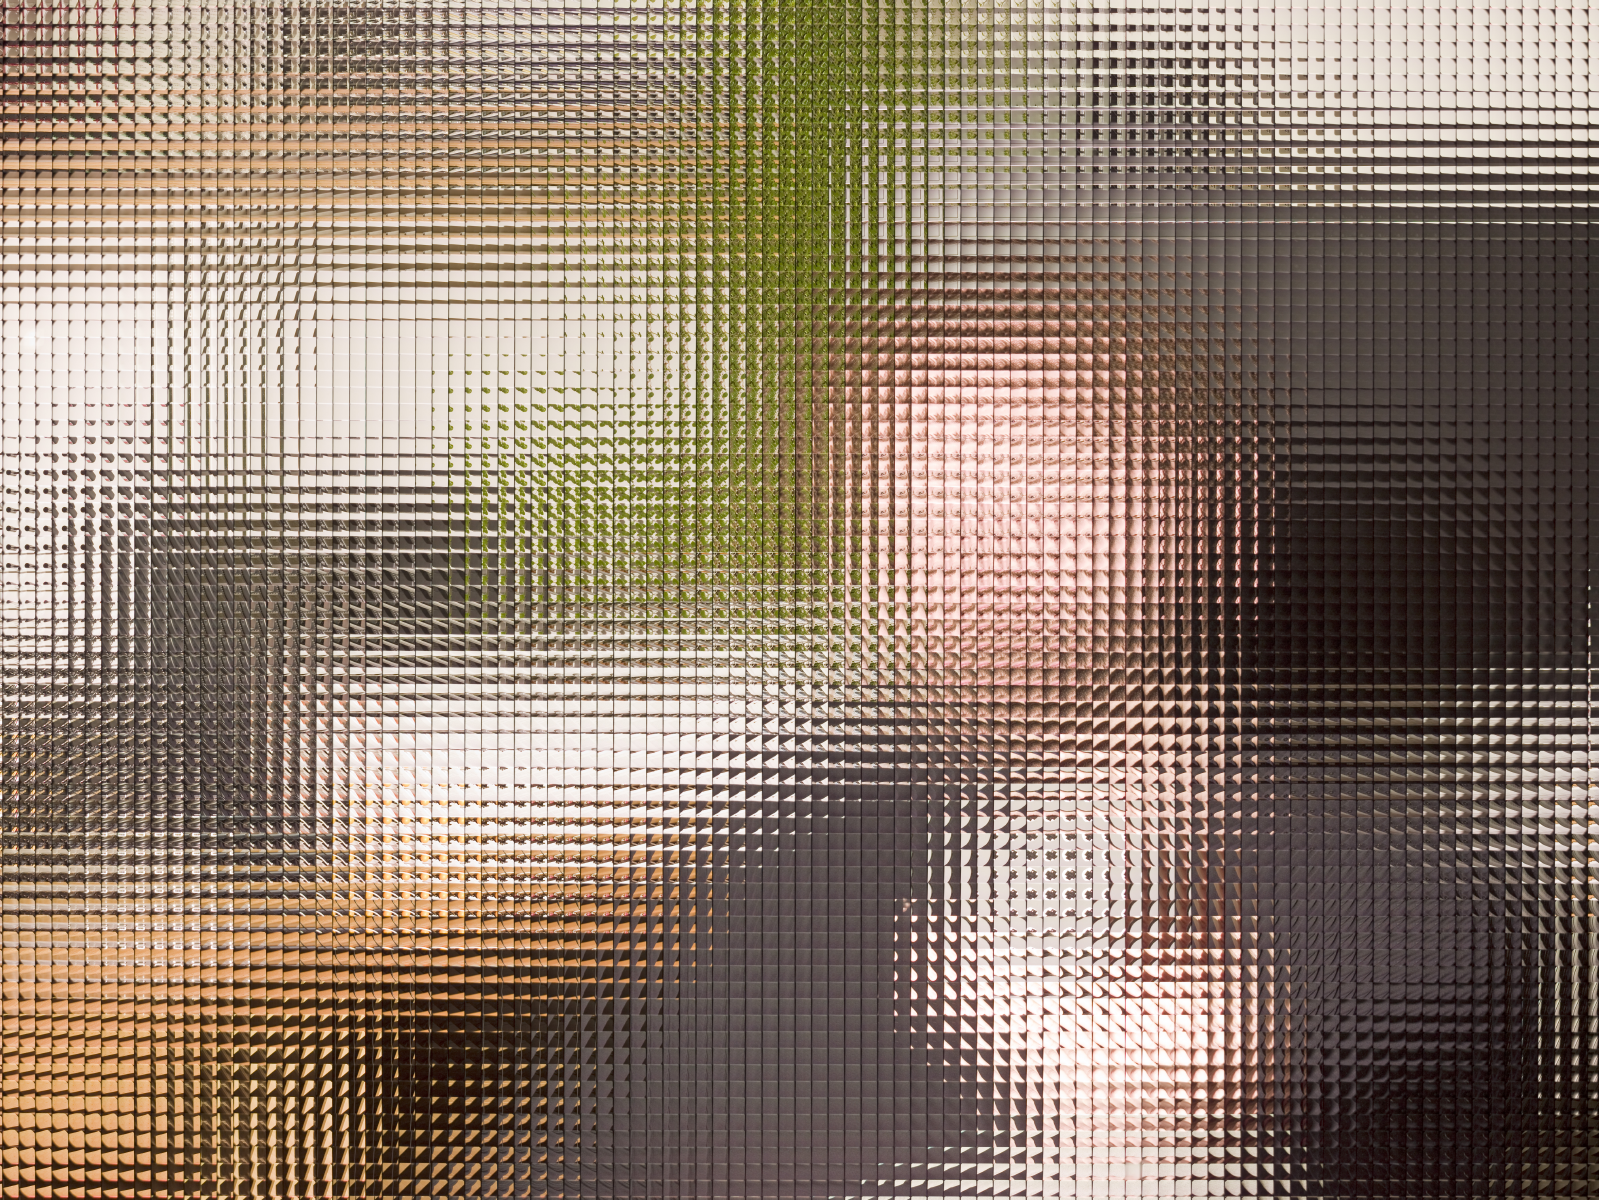
\includegraphics[angle=270,origin=b,width=0.35\textwidth]{472.eps}
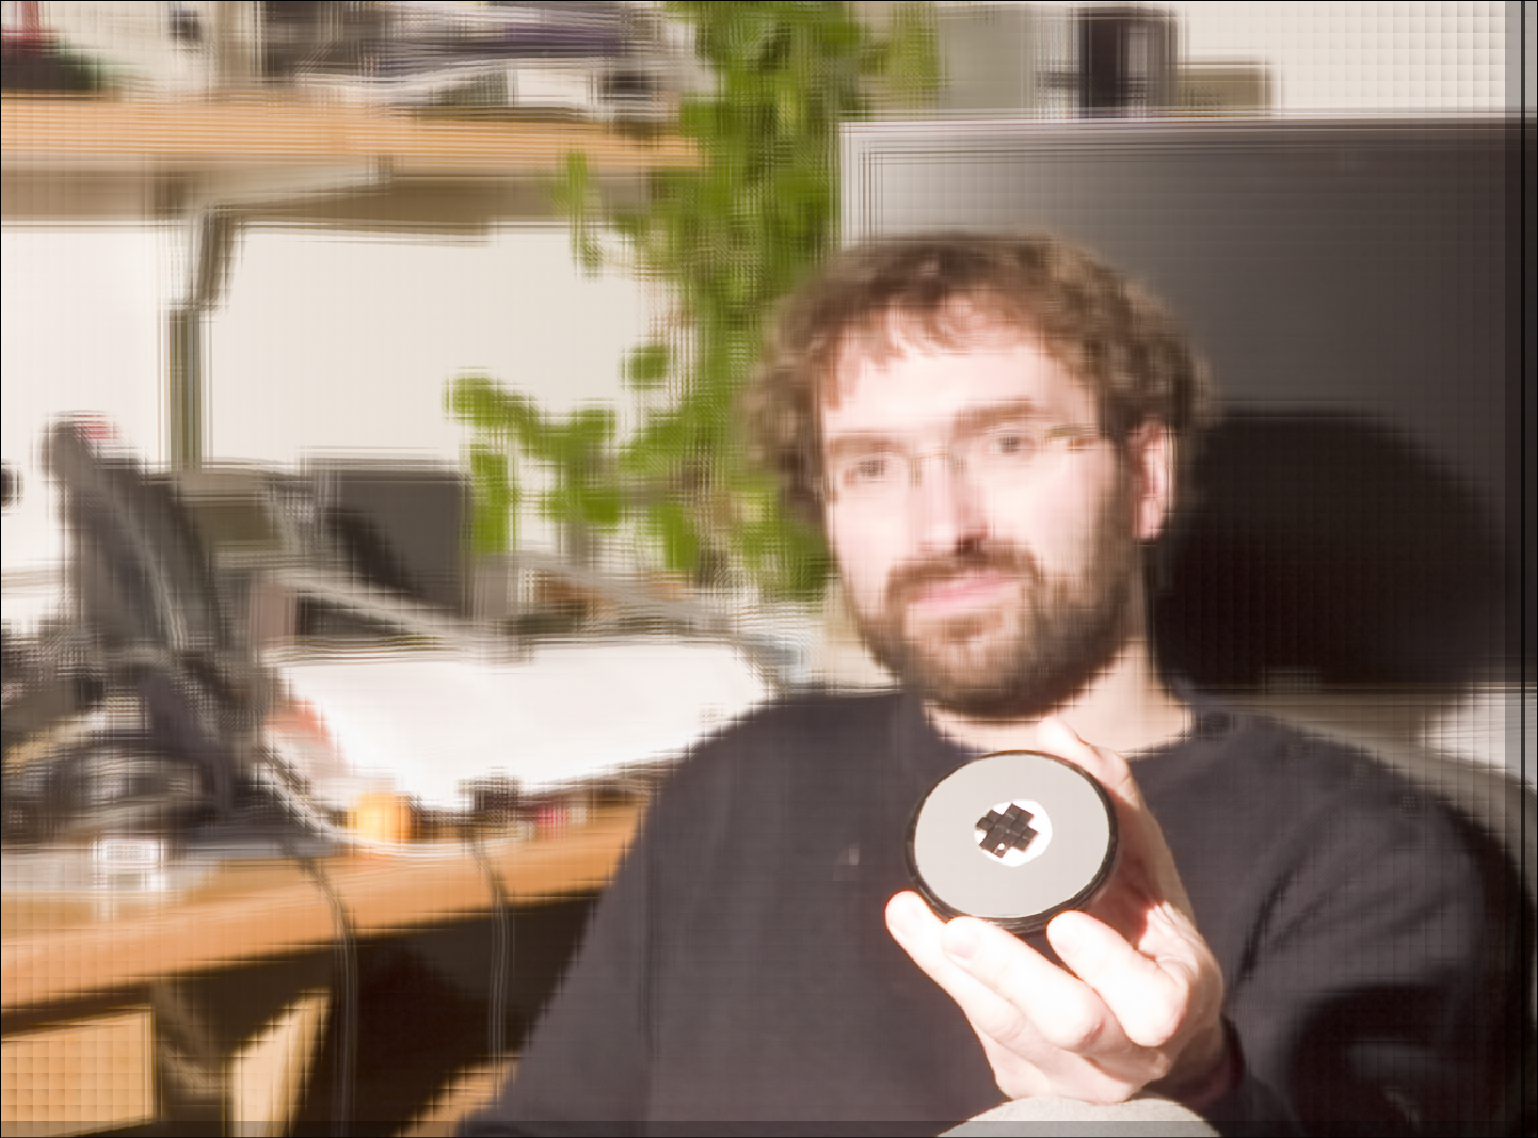
\includegraphics[angle=270,origin=b,width=0.35\textwidth]{gather.eps}
\caption{Gather}
\end{figure}

This is a rendering of light field image processing with a resolution of 7500x7500. Mapdist = 0 because it is not a regular stencil calculation.

\begin{screen}
\tiny
\begin{verbatim}
orig()
{
  ry = (R+ofs)*IM;
  rx = (R+ofs);
  int w, pix, cvalR, cvalG, cvalB;

  for (row=PAD; row<OM-PAD; row++) {
    for (col=PAD; col<OM-PAD; col++) {
       c = ((row>>4)*R + (((~row&15)*ofs)>>4))*IM
          + (col>>4)*R + (((~col&15)*ofs)>>4);
      cvalR=0;
      cvalG=0;
      cvalB=0;
      for (i=-1; i<=1; i++) {
        for (j=-1; j<=1; j++) {
          Uint pix = in[c+ry*i+rx*j];
          w = weight[WBASE+i*MAXDELTA*2+j];
          cvalR += ((pix>>24)&255)*w;
          cvalG += ((pix>>16)&255)*w;
          cvalB += ((pix>> 8)&255)*w;
          count0++;
        }
      }
      out0[row*OM+col] = ((cvalR>>8)<<24) | ((cvalG>>8)<<16) | ((cvalB>>8)<<8);
} } }
\end{verbatim}
\end{screen}

\begin{screen}
\tiny
\begin{verbatim}
imax()
{
  Ull CHIP;
  ry = (R+ofs)*IM;
  rx = (R+ofs);
  int w, pix, cvalR, cvalG, cvalB;

  for (row=0; row<RRANGE; row++) { /* 0..381 */
    for (CHIP=0; CHIP<NCHIP; CHIP++) {
      for (col=0; col<CRANGE; col++) {
        for (oc=0; oc<OMAP; oc++) {
          c =((((CHIP*OMAP+oc)*RRANGE+row+PAD)>>4)*R + (((~((CHIP*OMAP+oc)*RRANGE+row+PAD)&15)*ofs)>>4))*IM
            + ((                      col+PAD)>>4)*R + (((~(                      col+PAD)&15)*ofs)>>4);
          /* 256  512 256 */
          pix = in[c+ry*(-1)+rx*(-1)]; w = 16; cvalR =((pix>>24)&255)*w; cvalG =((pix>>16)&255)*w; cvalB =((pix>> 8)&255)*w;
          pix = in[c+ry*(-1)+rx*( 0)]; w = 32; cvalR+=((pix>>24)&255)*w; cvalG+=((pix>>16)&255)*w; cvalB+=((pix>> 8)&255)*w;
          pix = in[c+ry*(-1)+rx*( 1)]; w = 16; cvalR+=((pix>>24)&255)*w; cvalG+=((pix>>16)&255)*w; cvalB+=((pix>> 8)&255)*w;
          /* 512 1024 512 */
          pix = in[c+ry*( 0)+rx*(-1)]; w = 32; cvalR+=((pix>>24)&255)*w; cvalG+=((pix>>16)&255)*w; cvalB+=((pix>> 8)&255)*w;
          pix = in[c+ry*( 0)+rx*( 0)]; w = 64; cvalR+=((pix>>24)&255)*w; cvalG+=((pix>>16)&255)*w; cvalB+=((pix>> 8)&255)*w;
          pix = in[c+ry*( 0)+rx*( 1)]; w = 32; cvalR+=((pix>>24)&255)*w; cvalG+=((pix>>16)&255)*w; cvalB+=((pix>> 8)&255)*w;
          /* 256  512 256 */
          pix = in[c+ry*( 1)+rx*(-1)]; w = 16; cvalR+=((pix>>24)&255)*w; cvalG+=((pix>>16)&255)*w; cvalB+=((pix>> 8)&255)*w;
          pix = in[c+ry*( 1)+rx*( 0)]; w = 32; cvalR+=((pix>>24)&255)*w; cvalG+=((pix>>16)&255)*w; cvalB+=((pix>> 8)&255)*w;
          pix = in[c+ry*( 1)+rx*( 1)]; w = 16; cvalR+=((pix>>24)&255)*w; cvalG+=((pix>>16)&255)*w; cvalB+=((pix>> 8)&255)*w;
          count1+=9;
          out1[((CHIP*OMAP+oc)*RRANGE+row+PAD)*OM+(col+PAD)] = ((cvalR>>8)<<24) | ((cvalG>>8)<<16) | ((cvalB>>8)<<8);
} } } } }
\end{verbatim}
\end{screen}

\begin{screen}
\tiny
\begin{verbatim}
imax()
{
  Ull  CHIP;  Ull  LOOP1, LOOP0;  Ull  INIT1, INIT0;
  Ull  AR[64][4];                     /* output of EX     in each unit */
  Ull  BR[64][4][4];                  /* output registers in each unit */
  Ull  r0, r1, r2, r3, r4, r5, r6, r7, r8, r9, r10, r11, r12, r13, r14, r15;
  Ull  r16, r17, r18, r19, r20, r21, r22, r23, r24, r25, r26, r27, r28, r29, r30, r31;
  Ull  c0, c1, c2, c3, ex0, ex1;  Ull  x[NCHIP];
  ry = (R+ofs)*IM;  rx = (R+ofs);
  Uint *ym_xm   = in         -ry-rx;
     :
  for (row=RRANGE-1; row>=0; row--) {
    int yin0[NCHIP];
    Uint *acci_ym0[NCHIP];    Uint *acci_yz0[NCHIP];    Uint *acci_yp0[NCHIP];
    Uint *acco_base0[NCHIP];  Uint *acco0[NCHIP];
         :
    Uint *acco_base5[NCHIP];  Uint *acco5[NCHIP];
    for (CHIP=0; CHIP<NCHIP; CHIP++) {
      int row0 = (CHIP*OMAP+0)*RRANGE+row+PAD;
      int yout0 = row0*OM;
      yin0[CHIP] = ((row0>>4)*R + (((~row0&15)*ofs)>>4))*IM;
      acci_ym0[CHIP] = in+yin0[CHIP]     -ry;      acci_yz0[CHIP] = in+yin0[CHIP];      acci_yp0[CHIP] = in+yin0[CHIP]     +ry;
      acco_base0[CHIP] = out1+yout0+PAD;  acco0[CHIP] = out1+yout0+PAD;
        :
      acco_base5[CHIP] = out1+yout5+PAD;  acco5[CHIP] = out1+yout5+PAD;
    }
//EMAX5A begin gather mapdist=0
    for (CHIP=0; CHIP<NCHIP; CHIP++) {
      for (INIT0=1,LOOP0=CRANGE,x[CHIP]=PAD-1; LOOP0--; INIT0=0) {
        exe(OP_ADD,  &x[CHIP], x[CHIP],  EXP_H3210,         1LL, EXP_H3210, 0LL, EXP_H3210, OP_NOP,   0LL, OP_NOP, 0LL);     /* stage#0 */
        exe(OP_SUB,  &r1,         -1LL,  EXP_H3210,     x[CHIP], EXP_H3210, 0LL, EXP_H3210, OP_AND,  15LL, OP_NOP, 0LL);     /* stage#1 */
        exe(OP_NOP,  &r2,      x[CHIP],  EXP_H3210,         0LL, EXP_H3210, 0LL, EXP_H3210, OP_OR,    0LL, OP_SRL, 4LL);     /* stage#1 */
        exe(OP_MLUH, &r3,           r1,  EXP_H3210,    (Ull)ofs, EXP_H3210, 0LL, EXP_H3210, OP_OR,    0LL, OP_SRL, 4LL);     /* stage#2 */
        exe(OP_MLUH, &r4,           r2,  EXP_H3210,        75LL, EXP_H3210, 0LL, EXP_H3210, OP_NOP,   0LL, OP_NOP, 0LL);     /* stage#2 */
        exe(OP_ADD3, &r0,           r3,  EXP_H3210,          r4, EXP_H3210,(Ull)yin0[CHIP], EXP_H3210,OP_OR,0LL,OP_SLL, 2LL);/* stage#3 */
        exe(OP_ADD,  &r1,           r3,  EXP_H3210,          r4, EXP_H3210, 0LL, EXP_H3210, OP_OR,    0LL, OP_NOP, 0LL);     /* stage#3 */
        mop(OP_LDWR,    1, &BR[4][0][1],  r0, (Ull)ym_xm, MSK_D0, (Ull)acci_ym0[CHIP], IM, 0, 0, (Ull)NULL, IM);         /* stage#4 */
        mop(OP_LDWR,    1, &BR[4][1][1],  r0, (Ull)ym_xz, MSK_D0, (Ull)acci_ym0[CHIP], IM, 0, 0, (Ull)NULL, IM);         /* stage#4 */
        mop(OP_LDWR,    1, &BR[4][2][1],  r0, (Ull)ym_xp, MSK_D0, (Ull)acci_ym0[CHIP], IM, 0, 0, (Ull)NULL, IM);         /* stage#4 */
        exe(OP_MLUH,  &r10,     BR[4][0][1],  EXP_B5410,        16LL, EXP_H3210, 0LL, EXP_H3210, OP_NOP,  0LL, OP_NOP, 0LL); /* stage#5 */
        exe(OP_MLUH,  &r11,     BR[4][1][1],  EXP_B5410,        32LL, EXP_H3210, 0LL, EXP_H3210, OP_NOP,  0LL, OP_NOP, 0LL); /* stage#5 */
        exe(OP_MLUH,  &r12,     BR[4][2][1],  EXP_B5410,        16LL, EXP_H3210, 0LL, EXP_H3210, OP_NOP,  0LL, OP_NOP, 0LL); /* stage#5 */
        exe(OP_MLUH,  &r13,     BR[4][0][1],  EXP_B7632,        16LL, EXP_H3210, 0LL, EXP_H3210, OP_NOP,  0LL, OP_NOP, 0LL); /* stage#6 */
        exe(OP_MLUH,  &r14,     BR[4][1][1],  EXP_B7632,        32LL, EXP_H3210, 0LL, EXP_H3210, OP_NOP,  0LL, OP_NOP, 0LL); /* stage#6 */
        exe(OP_MLUH,  &r15,     BR[4][2][1],  EXP_B7632,        16LL, EXP_H3210, 0LL, EXP_H3210, OP_NOP,  0LL, OP_NOP, 0LL); /* stage#6 */
        exe(OP_MAUH3, &r20,  r10, EXP_H3210,  r11, EXP_H3210,  r12, EXP_H3210, OP_NOP, 0LL, OP_NOP, 0LL);                    /* stage#6 */
        mop(OP_LDWR,    1, &BR[6][0][1], r0, (Ull)yz_xm, MSK_D0, (Ull)acci_yz0[CHIP], IM, 0, 0, (Ull)NULL, IM);          /* stage#6 */
        mop(OP_LDWR,    1, &BR[6][1][1], r0, (Ull)yz_xz, MSK_D0, (Ull)acci_yz0[CHIP], IM, 0, 0, (Ull)NULL, IM);          /* stage#6 */
        mop(OP_LDWR,    1, &BR[6][2][1], r0, (Ull)yz_xp, MSK_D0, (Ull)acci_yz0[CHIP], IM, 0, 0, (Ull)NULL, IM);          /* stage#6 */
        exe(OP_MAUH3, &r21,  r13, EXP_H3210,  r14, EXP_H3210,  r15, EXP_H3210, OP_NOP, 0LL, OP_NOP, 0LL);                    /* stage#7 */
        exe(OP_MLUH,  &r10,     BR[6][0][1],  EXP_B5410,        32LL, EXP_H3210, 0LL, EXP_H3210, OP_NOP,  0LL, OP_NOP, 0LL); /* stage#7 */
        exe(OP_MLUH,  &r11,     BR[6][1][1],  EXP_B5410,        64LL, EXP_H3210, 0LL, EXP_H3210, OP_NOP,  0LL, OP_NOP, 0LL); /* stage#7 */
        exe(OP_MLUH,  &r12,     BR[6][2][1],  EXP_B5410,        32LL, EXP_H3210, 0LL, EXP_H3210, OP_NOP,  0LL, OP_NOP, 0LL); /* stage#7 */
        exe(OP_MLUH,  &r13,     BR[6][0][1],  EXP_B7632,        32LL, EXP_H3210, 0LL, EXP_H3210, OP_NOP,  0LL, OP_NOP, 0LL); /* stage#8 */
        exe(OP_MLUH,  &r14,     BR[6][1][1],  EXP_B7632,        64LL, EXP_H3210, 0LL, EXP_H3210, OP_NOP,  0LL, OP_NOP, 0LL); /* stage#8 */
        exe(OP_MLUH,  &r15,     BR[6][2][1],  EXP_B7632,        32LL, EXP_H3210, 0LL, EXP_H3210, OP_NOP,  0LL, OP_NOP, 0LL); /* stage#8 */
        exe(OP_MAUH3, &r22,  r10, EXP_H3210,  r11, EXP_H3210,  r12, EXP_H3210, OP_NOP, 0LL, OP_NOP, 0LL);                    /* stage#8 */
        mop(OP_LDWR,    1, &BR[8][0][1], r0, (Ull)yp_xm, MSK_D0, (Ull)acci_yp0[CHIP], IM, 0, 0, (Ull)NULL, IM);          /* stage#8 */
        mop(OP_LDWR,    1, &BR[8][1][1], r0, (Ull)yp_xz, MSK_D0, (Ull)acci_yp0[CHIP], IM, 0, 0, (Ull)NULL, IM);          /* stage#8 */
        mop(OP_LDWR,    1, &BR[8][2][1], r0, (Ull)yp_xp, MSK_D0, (Ull)acci_yp0[CHIP], IM, 0, 0, (Ull)NULL, IM);          /* stage#8 */
        exe(OP_MAUH3, &r23,  r13, EXP_H3210,  r14, EXP_H3210,  r15, EXP_H3210, OP_NOP, 0LL, OP_NOP, 0LL);                    /* stage#9 */
        exe(OP_MLUH,  &r10,     BR[8][0][1],  EXP_B5410,        16LL, EXP_H3210, 0LL, EXP_H3210, OP_NOP,  0LL, OP_NOP, 0LL); /* stage#9 */
        exe(OP_MLUH,  &r11,     BR[8][1][1],  EXP_B5410,        32LL, EXP_H3210, 0LL, EXP_H3210, OP_NOP,  0LL, OP_NOP, 0LL); /* stage#9 */
        exe(OP_MLUH,  &r12,     BR[8][2][1],  EXP_B5410,        16LL, EXP_H3210, 0LL, EXP_H3210, OP_NOP,  0LL, OP_NOP, 0LL); /* stage#9 */
        exe(OP_MLUH,  &r13,     BR[8][0][1],  EXP_B7632,        16LL, EXP_H3210, 0LL, EXP_H3210, OP_NOP,  0LL, OP_NOP, 0LL); /* stage#10 */
        exe(OP_MLUH,  &r14,     BR[8][1][1],  EXP_B7632,        32LL, EXP_H3210, 0LL, EXP_H3210, OP_NOP,  0LL, OP_NOP, 0LL); /* stage#10 */
        exe(OP_MLUH,  &r15,     BR[8][2][1],  EXP_B7632,        16LL, EXP_H3210, 0LL, EXP_H3210, OP_NOP,  0LL, OP_NOP, 0LL); /* stage#10 */
        exe(OP_MAUH3, &r24,  r10, EXP_H3210,  r11, EXP_H3210,  r12, EXP_H3210, OP_NOP, 0LL, OP_NOP, 0LL);                    /* stage#10 */
        exe(OP_MAUH3, &r25,  r13, EXP_H3210,  r14, EXP_H3210,  r15, EXP_H3210, OP_NOP, 0LL, OP_NOP, 0LL);                    /* stage#11 */
        exe(OP_MAUH3, &r30,  r20, EXP_H3210,  r22, EXP_H3210,  r24, EXP_H3210, OP_AND, -1LL, OP_SRLM, 8LL);                  /* stage#12 */
        exe(OP_MAUH3, &r31,  r21, EXP_H3210,  r23, EXP_H3210,  r25, EXP_H3210, OP_AND, -1LL, OP_SRLM, 8LL);                  /* stage#12 */
        exe(OP_MH2BW, &r29,  r31, EXP_H3210,  r30, EXP_H3210,  0LL, EXP_H3210, OP_NOP,  0LL, OP_NOP, 0LL);                   /* stage#13 */
        mop(OP_STWR,    3, &r29, (Ull)(acco0[CHIP]++), 0LL, MSK_D0, (Ull)acco_base0[CHIP], CRANGE, 0,0,(Ull)NULL,CRANGE);/* stage#13 */
        :
        /**********************/
        exe(OP_ADD,  &r0,           r1,  EXP_H3210,   (Ull)yin5[CHIP], EXP_H3210, 0LL, EXP_H3210, OP_OR,   0LL, OP_SLL, 2LL); /* stage#53 */
        /**********************/
        mop(OP_LDWR,    1, &BR[54][0][1],  r0, (Ull)ym_xm, MSK_D0, (Ull)acci_ym5[CHIP], IM, 0, 0, (Ull)NULL, IM);         /* stage#54 */
        mop(OP_LDWR,    1, &BR[54][1][1],  r0, (Ull)ym_xz, MSK_D0, (Ull)acci_ym5[CHIP], IM, 0, 0, (Ull)NULL, IM);         /* stage#54 */
        mop(OP_LDWR,    1, &BR[54][2][1],  r0, (Ull)ym_xp, MSK_D0, (Ull)acci_ym5[CHIP], IM, 0, 0, (Ull)NULL, IM);         /* stage#54 */
        exe(OP_MLUH,  &r10,     BR[54][0][1],  EXP_B5410,        16LL, EXP_H3210, 0LL, EXP_H3210, OP_NOP,  0LL, OP_NOP, 0LL); /* stage#55 */
        exe(OP_MLUH,  &r11,     BR[54][1][1],  EXP_B5410,        32LL, EXP_H3210, 0LL, EXP_H3210, OP_NOP,  0LL, OP_NOP, 0LL); /* stage#55 */
        exe(OP_MLUH,  &r12,     BR[54][2][1],  EXP_B5410,        16LL, EXP_H3210, 0LL, EXP_H3210, OP_NOP,  0LL, OP_NOP, 0LL); /* stage#55 */
        exe(OP_MLUH,  &r13,     BR[54][0][1],  EXP_B7632,        16LL, EXP_H3210, 0LL, EXP_H3210, OP_NOP,  0LL, OP_NOP, 0LL); /* stage#56 */
        exe(OP_MLUH,  &r14,     BR[54][1][1],  EXP_B7632,        32LL, EXP_H3210, 0LL, EXP_H3210, OP_NOP,  0LL, OP_NOP, 0LL); /* stage#56 */
        exe(OP_MLUH,  &r15,     BR[54][2][1],  EXP_B7632,        16LL, EXP_H3210, 0LL, EXP_H3210, OP_NOP,  0LL, OP_NOP, 0LL); /* stage#56 */
        exe(OP_MAUH3, &r20,  r10, EXP_H3210,  r11, EXP_H3210,  r12, EXP_H3210, OP_NOP, 0LL, OP_NOP, 0LL);                     /* stage#56 */
        mop(OP_LDWR,    1, &BR[56][0][1], r0, (Ull)yz_xm, MSK_D0, (Ull)acci_yz5[CHIP], IM, 0, 0, (Ull)NULL, IM);          /* stage#56 */
        mop(OP_LDWR,    1, &BR[56][1][1], r0, (Ull)yz_xz, MSK_D0, (Ull)acci_yz5[CHIP], IM, 0, 0, (Ull)NULL, IM);          /* stage#56 */
        mop(OP_LDWR,    1, &BR[56][2][1], r0, (Ull)yz_xp, MSK_D0, (Ull)acci_yz5[CHIP], IM, 0, 0, (Ull)NULL, IM);          /* stage#56 */
        exe(OP_MAUH3, &r21,  r13, EXP_H3210,  r14, EXP_H3210,  r15, EXP_H3210, OP_NOP, 0LL, OP_NOP, 0LL);                     /* stage#57 */
        exe(OP_MLUH,  &r10,     BR[56][0][1],  EXP_B5410,        32LL, EXP_H3210, 0LL, EXP_H3210, OP_NOP,  0LL, OP_NOP, 0LL); /* stage#57 */
        exe(OP_MLUH,  &r11,     BR[56][1][1],  EXP_B5410,        64LL, EXP_H3210, 0LL, EXP_H3210, OP_NOP,  0LL, OP_NOP, 0LL); /* stage#57 */
        exe(OP_MLUH,  &r12,     BR[56][2][1],  EXP_B5410,        32LL, EXP_H3210, 0LL, EXP_H3210, OP_NOP,  0LL, OP_NOP, 0LL); /* stage#57 */
        exe(OP_MLUH,  &r13,     BR[56][0][1],  EXP_B7632,        32LL, EXP_H3210, 0LL, EXP_H3210, OP_NOP,  0LL, OP_NOP, 0LL); /* stage#58 */
        exe(OP_MLUH,  &r14,     BR[56][1][1],  EXP_B7632,        64LL, EXP_H3210, 0LL, EXP_H3210, OP_NOP,  0LL, OP_NOP, 0LL); /* stage#58 */
        exe(OP_MLUH,  &r15,     BR[56][2][1],  EXP_B7632,        32LL, EXP_H3210, 0LL, EXP_H3210, OP_NOP,  0LL, OP_NOP, 0LL); /* stage#58 */
        exe(OP_MAUH3, &r22,  r10, EXP_H3210,  r11, EXP_H3210,  r12, EXP_H3210, OP_NOP, 0LL, OP_NOP, 0LL);                     /* stage#58 */
        mop(OP_LDWR,    1, &BR[58][0][1], r0, (Ull)yp_xm, MSK_D0, (Ull)acci_yp5[CHIP], IM, 0, 0, (Ull)NULL, IM);          /* stage#58 */
        mop(OP_LDWR,    1, &BR[58][1][1], r0, (Ull)yp_xz, MSK_D0, (Ull)acci_yp5[CHIP], IM, 0, 0, (Ull)NULL, IM);          /* stage#58 */
        mop(OP_LDWR,    1, &BR[58][2][1], r0, (Ull)yp_xp, MSK_D0, (Ull)acci_yp5[CHIP], IM, 0, 0, (Ull)NULL, IM);          /* stage#58 */
        exe(OP_MAUH3, &r23,  r13, EXP_H3210,  r14, EXP_H3210,  r15, EXP_H3210, OP_NOP, 0LL, OP_NOP, 0LL);                     /* stage#59 */
        exe(OP_MLUH,  &r10,     BR[58][0][1],  EXP_B5410,        16LL, EXP_H3210, 0LL, EXP_H3210, OP_NOP,  0LL, OP_NOP, 0LL); /* stage#59 */
        exe(OP_MLUH,  &r11,     BR[58][1][1],  EXP_B5410,        32LL, EXP_H3210, 0LL, EXP_H3210, OP_NOP,  0LL, OP_NOP, 0LL); /* stage#59 */
        exe(OP_MLUH,  &r12,     BR[58][2][1],  EXP_B5410,        16LL, EXP_H3210, 0LL, EXP_H3210, OP_NOP,  0LL, OP_NOP, 0LL); /* stage#59 */
        exe(OP_MLUH,  &r13,     BR[58][0][1],  EXP_B7632,        16LL, EXP_H3210, 0LL, EXP_H3210, OP_NOP,  0LL, OP_NOP, 0LL); /* stage#60 */
        exe(OP_MLUH,  &r14,     BR[58][1][1],  EXP_B7632,        32LL, EXP_H3210, 0LL, EXP_H3210, OP_NOP,  0LL, OP_NOP, 0LL); /* stage#60 */
        exe(OP_MLUH,  &r15,     BR[58][2][1],  EXP_B7632,        16LL, EXP_H3210, 0LL, EXP_H3210, OP_NOP,  0LL, OP_NOP, 0LL); /* stage#60 */
        exe(OP_MAUH3, &r24,  r10, EXP_H3210,  r11, EXP_H3210,  r12, EXP_H3210, OP_NOP, 0LL, OP_NOP, 0LL);                     /* stage#60 */
        exe(OP_MAUH3, &r25,  r13, EXP_H3210,  r14, EXP_H3210,  r15, EXP_H3210, OP_NOP, 0LL, OP_NOP, 0LL);                     /* stage#61 */
        exe(OP_MAUH3, &r30,  r20, EXP_H3210,  r22, EXP_H3210,  r24, EXP_H3210, OP_AND, -1LL, OP_SRLM, 8LL); /* stage#62 */
        exe(OP_MAUH3, &r31,  r21, EXP_H3210,  r23, EXP_H3210,  r25, EXP_H3210, OP_AND, -1LL, OP_SRLM, 8LL); /* stage#62 */
        exe(OP_MH2BW, &r29,  r31, EXP_H3210,  r30, EXP_H3210,  0LL, EXP_H3210, OP_NOP,  0LL, OP_NOP, 0LL);  /* stage#63 */
        mop(OP_STWR,    3, &r29, (Ull)(acco5[CHIP]++), 0LL, MSK_D0, (Ull)acco_base5[CHIP], CRANGE, 0,0,(Ull)NULL, CRANGE);/* stage#63 */
    } }
//EMAX5A end
  }
//EMAX5A drain_dirty_lmm
}
\end{verbatim}
\end{screen}

\begin{figure}[htbp]
\center
\epsfile{file=gather+rmm-gather-emax6.eps,width=1.00\textwidth}
\caption{Lightfield rendering}
\end{figure}

\clearpage

\subsection{Lightfield distance image generation}

\shabox{
\leftline{cent\% make -f Makefile-csim.emax6+dma gdepth-csim.emax6+dma clean}
\leftline{cent\% ../../src/csim/csim -x gdepth-csim.emax6+dma}
}

\shabox{
\leftline{zynq\% make -f Makefile-zynq.emax6+dma gdepth-zynq.emax6+dma clean}
\leftline{zynq\% ./gdepth-zynq.emax6+dma}
}

\begin{figure}[htbp]
\center
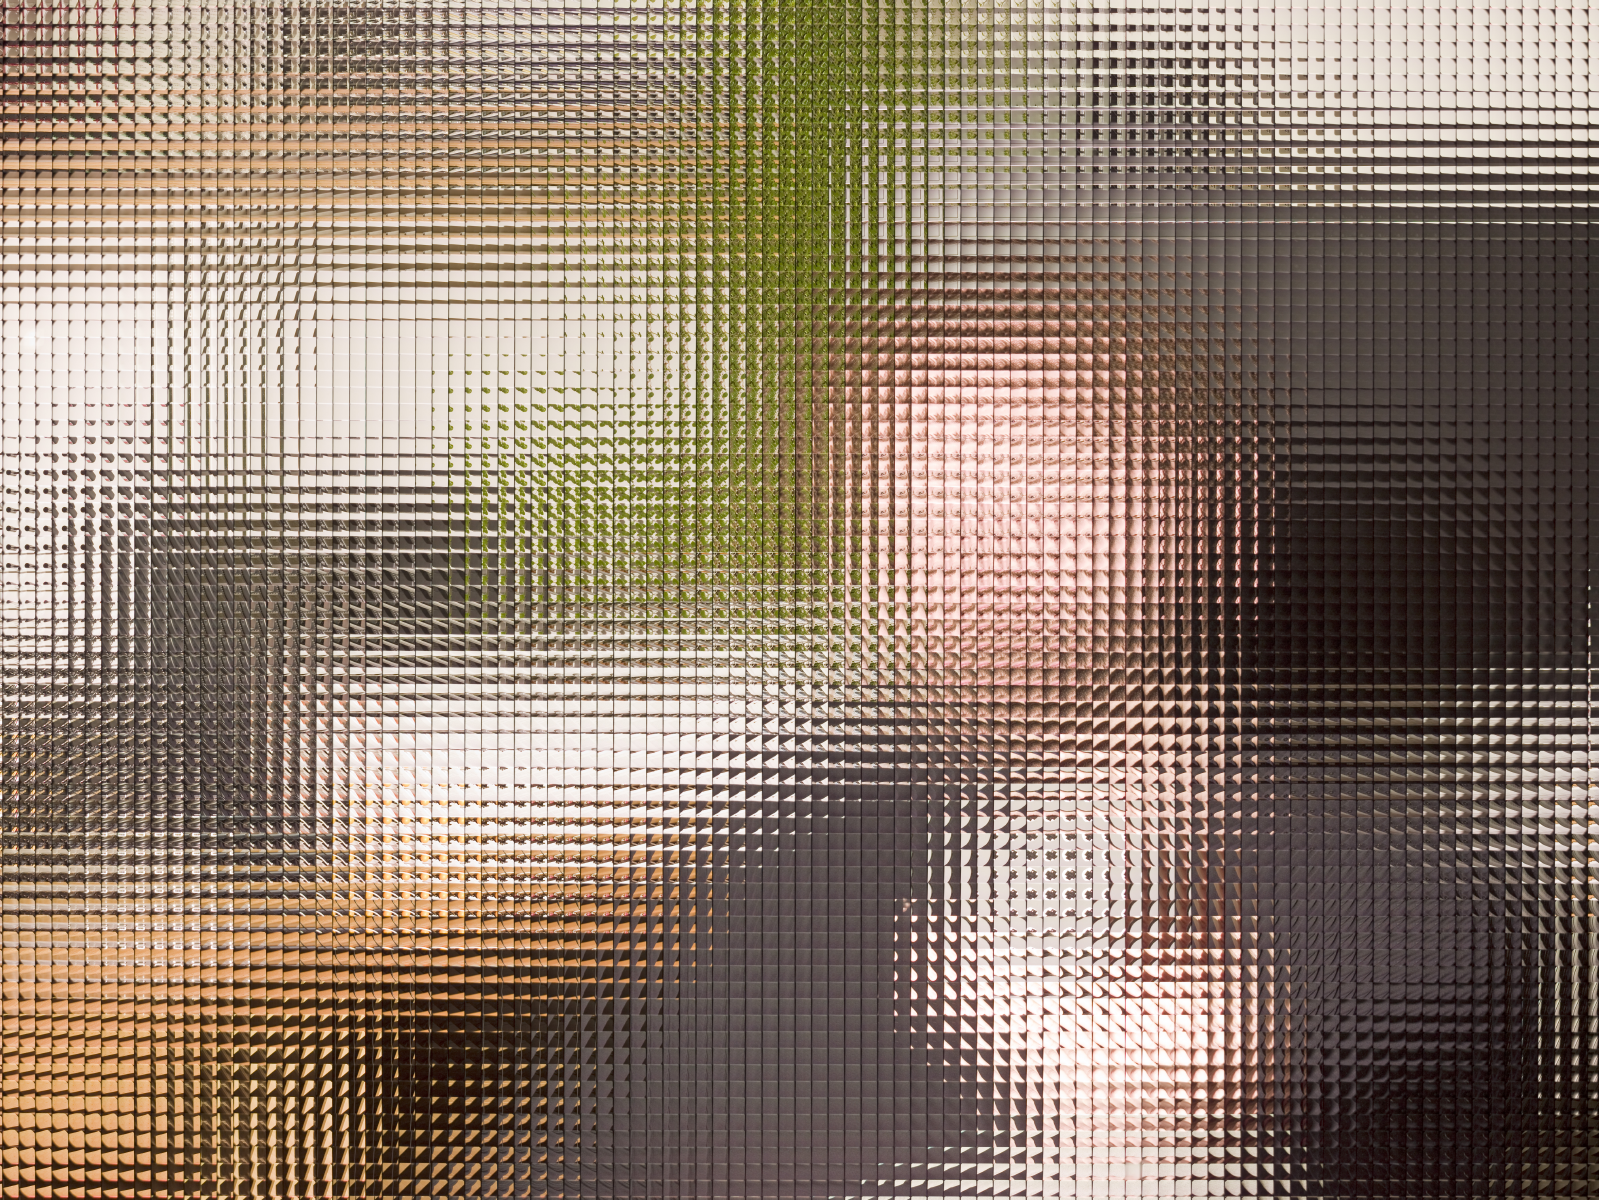
\includegraphics[angle=270,origin=b,width=0.35\textwidth]{472.eps}
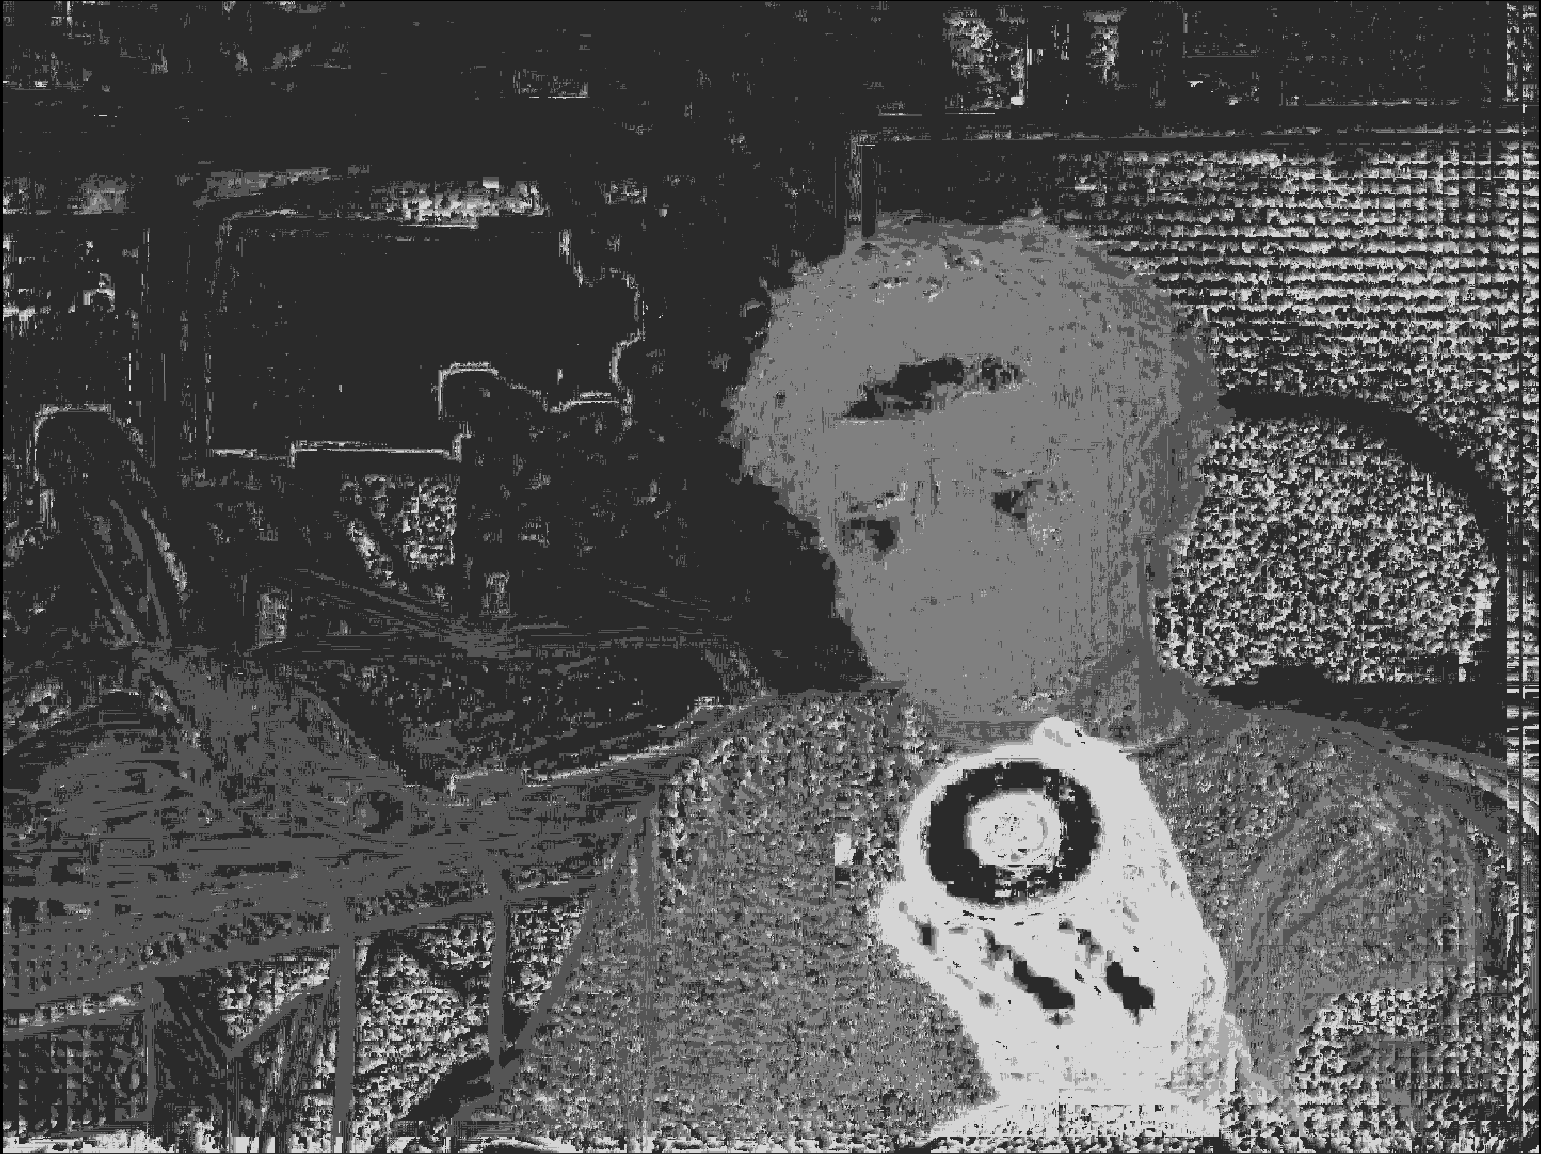
\includegraphics[angle=270,origin=b,width=0.35\textwidth]{gdepth.eps}
\caption{Gdepth}
\end{figure}

\begin{figure}[htbp]
\center
\includegraphics[width=0.80\textwidth]{lf0.eps}
\caption{\label{fig:lf0}Lightfield}
\end{figure}

This is a range image generation with resolution 7500 x 7500 light field
image processing. It uses an adaptive mapdist with a standard value mapdist
= 3, although it is not a regular stencil calculation.  Figure \ref
{fig:lf0} (a) shows the data structure of LF, (b) shows a 12x4 CGRA with one
Sum of absolute difference (SAD) calculator in each unit.  (b) shows the
data flow graph as in Figure \ref {fig:cnn0}. Suppose a microlens image of
75x75 pixels is arranged on a 100 x 100 grid point, and an image
(\textbf{in}) of 7500 x 7500 pixels is obtained in total.  For a part (3x3)
of each micro image (upside down, left and right), SAD is calculated between
multiple micro images separated by 75 + \textbf{ofs} pixels, and the minimum
\textbf{ofs} is generated as distance information
(\textbf{out}). Specifically, the SAD is calculated for 6 pixels of the 3x3
image at the center (\textbf{p0}) and 6 pixels of the 3x3 images at the 6
surrounding points (\textbf{p1}), and the SAD of a total of 36 pixels is
accumulated.  In the first stage of the CGRA (unit [0] [*]), the top row
(corresponding to i $\#$-1) of 3x3 pixels at the position of y $\#$ 0 is
assigned, six discrete loads (including p0 and p1) from the first LMM that
stores one row of images are performed (Dotted rectangle).  The second stage
(unit [1] [*]) and the third stage (unit [2] [*]) load from the locations
(p1) of y $\#$-1 and y $\#$ 1, respectively. And compare it with p0 obtained
in the first stage. After passing through 9 stages of the CGRA, four more
SADs are accumulated into one SAD using two more stages.  In the outermost
loop, change \textbf{ofs}, save the past minimum sad, and if a smaller SAD
value is obtained, update sad and out using the conditional store.  In this
way, 11 stages are used to calculate the SAD value of 36 pixels, and 40 of
44 arithmetic units are active.  The total number of stages is 18 stages
which includes 12 storage stage shown in (b) and 6 stages required for
address calculation as shown in c.  (c) is an implementation in which the
screen is divided into N chips, the input image is processed in parallel,
and each chip has the number of stages that can map the SAD operation of 36
pixels to the REP group.  Note that the outermost loop that updates ofs is
omitted. The theoretical number of cycles required for the above calculation
is 40xOM$^2$/(REPxN ).  Although 6 pixels from p0 and 36 pixels from p1 are
required to generate one pixel out, the theoretical transfer amount between
DDR and LMM is in: 9xOM$^2$ + out: OM$^2$ (The whole input image is IM$^2$,
but the amount referred to as in is 9xOM$^2$).

\begin{screen}
\tiny
\begin{verbatim}
orig()
{
  ry = (R+ofs)*IM;
  rx = (R+ofs); /* ofs: from 8 to 14 */
  for (row=PAD; row<OM-PAD; row++) {
    for (col=PAD; col<OM-PAD; col++) {
      c =((row>>4)*R + (((~row&15)*ofs)>>4))*IM
        + (col>>4)*R + (((~col&15)*ofs)>>4);
      s = 0;
      for (y=-1; y<=1; y++) {
        for (x=-1; x<=1; x++) {
          if (x == 0) continue;
          for (i=-1; i<=1; i++) {
            for (j=-1; j<=1; j++) {
              if (j == 0) continue;
              p0 = in[c     +(i*IM)     +j]; /* center */
              p1 = in[c+ry*y+(i*IM)+rx*x+j]; /* comparand */
              s += dif(p0, p1);
              if (s > 0xffff) s = 0xffff;
              count0++;
      } } } }
      if (sad0[row*OM+col]>TH && s<sad0[row*OM+col]) {
        sad0[row*OM+col] = s;
        out0[row*OM+col] = ofs;
} } } }
\end{verbatim}
\end{screen}

\begin{screen}
\tiny
\begin{verbatim}
imax()
{
  Ull CHIP;
  ry = (R+ofs)*IM;
  rx = (R+ofs); /* ofs: from 8 to 14 */
  for (row=0; row<RRANGE; row++) { /* 0..381 */
    for (CHIP=0; CHIP<NCHIP; CHIP++) {
      for (col=0; col<CRANGE; col++) {
        for (oc=0; oc<OMAP; oc++) {
          c =((((CHIP*OMAP+oc)*RRANGE+row+PAD)>>4)*R + (((~((CHIP*OMAP+oc)*RRANGE+row+PAD)&15)*ofs)>>4))*IM
            + ((                      col+PAD)>>4)*R + (((~(                      col+PAD)&15)*ofs)>>4);
          s = 0;
          for (y=-1; y<=1; y++) {
            for (x=-1; x<=1; x++) {
              if (x == 0) continue;
              for (i=-1; i<=1; i++) {
                for (j=-1; j<=1; j++) {
                  if (j == 0) continue;
                  p0 = in[c     +(i*IM)     +j]; /* center */
                  p1 = in[c+ry*y+(i*IM)+rx*x+j]; /* comparand */
                  s += dif(p0, p1);
                  count1++;
          } } } }
          if (sad1[((CHIP*OMAP+oc)*RRANGE+row+PAD)*OM+(col)+PAD]>TH && s<sad1[((CHIP*OMAP+oc)*RRANGE+row+PAD)*OM+(col+PAD)]) {
            sad1[((CHIP*OMAP+oc)*RRANGE+row+PAD)*OM+(col+PAD)] = s;
            out1[((CHIP*OMAP+oc)*RRANGE+row+PAD)*OM+(col+PAD)] = ofs;
} } } } } }
\end{verbatim}
\end{screen}

\begin{screen}
\tiny
\begin{verbatim}
imax()
{
  Ull  CHIP;  Ull  LOOP1, LOOP0;  Ull  INIT1, INIT0;
  Ull  AR[64][4];                     /* output of EX     in each unit */
  Ull  BR[64][4][4];                  /* output registers in each unit */
  Ull  r0, r1, r2, r3, r4, r5, r6, r7, r8, r9, r10, r11, r12, r13, r14, r15;
  Ull  r16, r17, r18, r19, r20, r21, r22, r23, r24, r25, r26, r27, r28, r29, r30, r31;
  Ull  c0, c1, c2, c3, ex0, ex1;  Ull  x[NCHIP];
  ry = (R+ofs)*IM; rx = (R+ofs);
  Uint *yzm_xm_m4 = in-IM   -rx-1;  Uint *yzm_xm_p4 = in-IM   -rx+1;
    :
  Uint *ypp_xp_m4 = in+IM+ry+rx-1;  Uint *ypp_xp_p4 = in+IM+ry+rx+1;
  for (row=RRANGE-1; row>=0; row--) {
    int  yin0[NCHIP];
    Uint *acci_yzm0[NCHIP];  Uint *acci_ymm0[NCHIP];  Uint *acci_ypm0[NCHIP];
    Uint *acci_yzz0[NCHIP];  Uint *acci_ymz0[NCHIP];  Uint *acci_ypz0[NCHIP];
    Uint *acci_yzp0[NCHIP];  Uint *acci_ymp0[NCHIP];  Uint *acci_ypp0[NCHIP];
    Uint *sadx_base0[NCHIP]; Uint *sadi0[NCHIP]; Uint *sado0[NCHIP];
    Uint *acco_base0[NCHIP]; Uint *acco0[NCHIP];
      :
    Uint *sadi_base0[NCHIP];  Uint *sadi0[NCHIP]; Uint *sado_base0[NCHIP];  Uint *sado0[NCHIP]; Uint *acco_base0[NCHIP];  Uint *acco0[NCHIP];
      :
    for (CHIP=0; CHIP<NCHIP; CHIP++) {
      yin0[CHIP] = ((row0>>4)*R + (((~row0&15)*ofs)>>4))*IM;
      acci_yzm0[CHIP] = in+yin0[CHIP]-IM;  acci_ymm0[CHIP] = in+yin0[CHIP]-IM-ry;  acci_ypm0[CHIP] = in+yin0[CHIP]-IM+ry;
      acci_yzz0[CHIP] = in+yin0[CHIP];     acci_ymz0[CHIP] = in+yin0[CHIP]   -ry;  acci_ypz0[CHIP] = in+yin0[CHIP]   +ry;
      acci_yzp0[CHIP] = in+yin0[CHIP]+IM;  acci_ymp0[CHIP] = in+yin0[CHIP]+IM-ry;  acci_ypp0[CHIP] = in+yin0[CHIP]+IM+ry;
      sadx_base0[CHIP] = sad1+yout0+PAD;  sadi0[CHIP] = sad1+yout0+PAD;  sado0[CHIP] = sad1+yout0+PAD;
      acco_base0[CHIP] = out1+yout0+PAD;  acco0[CHIP] = out1+yout0+PAD;
        :
    }
//EMAX5A begin gdepth mapdist=3
    for (CHIP=0; CHIP<NCHIP; CHIP++) {
      for (INIT0=1,LOOP0=CRANGE,x[CHIP]=PAD-1; LOOP0--; INIT0=0) {
        exe(OP_ADD,  &x[CHIP], x[CHIP],  EXP_H3210,        1LL, EXP_H3210, 0LL, EXP_H3210, OP_NOP,   0LL, OP_NOP, 0LL);   /* stage#0 */
        exe(OP_SUB,  &r1,         -1LL,  EXP_H3210,    x[CHIP], EXP_H3210, 0LL, EXP_H3210, OP_AND,  15LL, OP_NOP, 0LL);   /* stage#1 */
        exe(OP_NOP,  &r2,      x[CHIP],  EXP_H3210,        0LL, EXP_H3210, 0LL, EXP_H3210, OP_OR,    0LL, OP_SRL, 4LL);   /* stage#1 */
        exe(OP_MLUH, &r3,           r1,  EXP_H3210,   (Ull)ofs, EXP_H3210, 0LL, EXP_H3210, OP_OR,    0LL, OP_SRL, 4LL);   /* stage#2 */
        exe(OP_MLUH, &r4,           r2,  EXP_H3210,       75LL, EXP_H3210, 0LL, EXP_H3210, OP_NOP,   0LL, OP_NOP, 0LL);   /* stage#2 */
        exe(OP_ADD3, &r0,           r3,  EXP_H3210,         r4, EXP_H3210,(Ull)yin0[CHIP],EXP_H3210,OP_OR,0LL,OP_SLL,2LL);/* stage#3 */
        exe(OP_ADD,  &r1,           r3,  EXP_H3210,         r4, EXP_H3210, 0LL, EXP_H3210, OP_OR,    0LL, OP_NOP, 0LL);   /* stage#3 */
        mop(OP_LDWR,   1, &BR[4][0][1], r0, (Ull)yzm_xm_m4, MSK_D0, (Ull)acci_yzm0[CHIP], IM, 0, 0, (Ull)NULL, IM);   /* stage#4 */
        mop(OP_LDWR,   1, &BR[4][0][0], r0, (Ull)yzm_xm_p4, MSK_D0, (Ull)acci_yzm0[CHIP], IM, 0, 0, (Ull)NULL, IM);   /* stage#4 */
        mop(OP_LDWR,   1, &BR[4][1][1], r0, (Ull)yzm_xz_m4, MSK_D0, (Ull)acci_yzm0[CHIP], IM, 0, 0, (Ull)NULL, IM);   /* stage#4 */
        mop(OP_LDWR,   1, &BR[4][1][0], r0, (Ull)yzm_xz_p4, MSK_D0, (Ull)acci_yzm0[CHIP], IM, 0, 0, (Ull)NULL, IM);   /* stage#4 */
        mop(OP_LDWR,   1, &BR[4][2][1], r0, (Ull)yzm_xp_m4, MSK_D0, (Ull)acci_yzm0[CHIP], IM, 0, 0, (Ull)NULL, IM);   /* stage#4 */
        mop(OP_LDWR,   1, &BR[4][2][0], r0, (Ull)yzm_xp_p4, MSK_D0, (Ull)acci_yzm0[CHIP], IM, 0, 0, (Ull)NULL, IM);   /* stage#4 */
        exe(OP_MSSAD,&r14,   0LL, EXP_H3210, BR[4][0][0], EXP_H3210, BR[4][1][0], EXP_H3210, OP_NOP, 0LL, OP_NOP, 0LL);   /* stage#5 */
        exe(OP_MSSAD,&r15,   0LL, EXP_H3210, BR[4][0][1], EXP_H3210, BR[4][1][1], EXP_H3210, OP_NOP, 0LL, OP_NOP, 0LL);   /* stage#5 */
        exe(OP_MSSAD,&r16,   0LL, EXP_H3210, BR[4][2][0], EXP_H3210, BR[4][1][0], EXP_H3210, OP_NOP, 0LL, OP_NOP, 0LL);   /* stage#5 */
        exe(OP_MSSAD,&r17,   0LL, EXP_H3210, BR[4][2][1], EXP_H3210, BR[4][1][1], EXP_H3210, OP_NOP, 0LL, OP_NOP, 0LL);   /* stage#5 */
        mop(OP_LDWR,   1, &BR[5][0][1], r0, (Ull)ymm_xm_m4, MSK_D0, (Ull)acci_ymm0[CHIP], IM, 0, 0, (Ull)NULL, IM);   /* stage#5 */
        mop(OP_LDWR,   1, &BR[5][0][0], r0, (Ull)ymm_xm_p4, MSK_D0, (Ull)acci_ymm0[CHIP], IM, 0, 0, (Ull)NULL, IM);   /* stage#5 */
        mop(OP_LDWR,   1, &BR[5][2][1], r0, (Ull)ymm_xp_m4, MSK_D0, (Ull)acci_ymm0[CHIP], IM, 0, 0, (Ull)NULL, IM);   /* stage#5 */
        mop(OP_LDWR,   1, &BR[5][2][0], r0, (Ull)ymm_xp_p4, MSK_D0, (Ull)acci_ymm0[CHIP], IM, 0, 0, (Ull)NULL, IM);   /* stage#5 */
          :
        exe(OP_MAUH, &r24,   r14, EXP_H3210,  r15, EXP_H3210, 0LL, EXP_H3210, OP_NOP,   0LL, OP_NOP, 0LL);                /* stage#14 */
        exe(OP_MAUH, &r26,   r16, EXP_H3210,  r17, EXP_H3210, 0LL, EXP_H3210, OP_NOP,   0LL, OP_NOP, 0LL);                /* stage#14 */
        exe(OP_MAUH, &r30,   r24, EXP_H3210,  r26, EXP_H3210, 0LL, EXP_H3210, OP_SUMHL, 0LL, OP_NOP, 0LL);                /* stage#15 */
        mop(OP_LDWR,   1, &BR[15][1][1], (Ull)(sadi0[CHIP]++),0LL, MSK_D0,(Ull)sadx_base0[CHIP], CRANGE,0,1,(Ull)NULL,CRANGE);/* stage#15 */
        exe(OP_CMP_LT, &c0, r30,           EXP_H3210, BR[15][1][1], EXP_H3210, 0LL, EXP_H3210, OP_NOP,        0LL, OP_NOP, 0LL);  /* stage#16 */
        exe(OP_CMP_GT, &c1, BR[15][1][1],  EXP_H3210,        137LL, EXP_H3210, 0LL, EXP_H3210, OP_NOP,        0LL, OP_NOP, 0LL);  /* stage#16 */
        exe(OP_NOP,    &r31, 0LL,          EXP_H3210,          0LL, EXP_H3210, 0LL, EXP_H3210, OP_OR,    (Ull)ofs, OP_NOP, 0LL);  /* stage#16 */
        cex(OP_CEXE,   &ex1,   0, 0, c1, c0, 0x8888);                                                                             /* stage#17 */
        mop(OP_STWR, ex1, &r31, (Ull)(acco0[CHIP]++), 0LL, MSK_D0, (Ull)acco_base0[CHIP], CRANGE, 0, 1, (Ull)NULL, CRANGE);   /* stage#17 */
        cex(OP_CEXE,   &ex0,   0, 0, c1, c0, 0x8888);                                                                             /* stage#17 */
        mop(OP_STWR, ex0, &r30, (Ull)(sado0[CHIP]++), 0LL, MSK_D0, (Ull)sadx_base0[CHIP], CRANGE, 0, 1, (Ull)NULL, CRANGE);   /* stage#17 */
        /********************/
        exe(OP_ADD,  &r0,           r1,  EXP_H3210,    (Ull)yin1[CHIP], EXP_H3210, 0LL, EXP_H3210, OP_OR,    0LL, OP_SLL, 2LL);   /* stage#17 */
        /********************/
          :
        exe(OP_MSSAD,&r24,   r14, EXP_H3210, BR[51][0][0], EXP_H3210, BR[49][1][0], EXP_H3210, OP_NOP, 0LL, OP_NOP, 0LL); /* stage#52 */
        exe(OP_MSSAD,&r25,   r15, EXP_H3210, BR[51][0][1], EXP_H3210, BR[49][1][1], EXP_H3210, OP_NOP, 0LL, OP_NOP, 0LL); /* stage#52 */
        exe(OP_MSSAD,&r26,   r16, EXP_H3210, BR[51][2][0], EXP_H3210, BR[49][1][0], EXP_H3210, OP_NOP, 0LL, OP_NOP, 0LL); /* stage#52 */
        exe(OP_MSSAD,&r27,   r17, EXP_H3210, BR[51][2][1], EXP_H3210, BR[49][1][1], EXP_H3210, OP_NOP, 0LL, OP_NOP, 0LL); /* stage#52 */
        mop(OP_LDWR,   1, &BR[52][0][1], r0, (Ull)yzp_xm_m4, MSK_D0, (Ull)acci_yzp3[CHIP], IM, 0, 0, (Ull)NULL, IM);  /* stage#52 */
        mop(OP_LDWR,   1, &BR[52][0][0], r0, (Ull)yzp_xm_p4, MSK_D0, (Ull)acci_yzp3[CHIP], IM, 0, 0, (Ull)NULL, IM);  /* stage#52 */
        mop(OP_LDWR,   1, &BR[52][1][1], r0, (Ull)yzp_xz_m4, MSK_D0, (Ull)acci_yzp3[CHIP], IM, 0, 0, (Ull)NULL, IM);  /* stage#52 */
        mop(OP_LDWR,   1, &BR[52][1][0], r0, (Ull)yzp_xz_p4, MSK_D0, (Ull)acci_yzp3[CHIP], IM, 0, 0, (Ull)NULL, IM);  /* stage#52 */
        mop(OP_LDWR,   1, &BR[52][2][1], r0, (Ull)yzp_xp_m4, MSK_D0, (Ull)acci_yzp3[CHIP], IM, 0, 0, (Ull)NULL, IM);  /* stage#52 */
        mop(OP_LDWR,   1, &BR[52][2][0], r0, (Ull)yzp_xp_p4, MSK_D0, (Ull)acci_yzp3[CHIP], IM, 0, 0, (Ull)NULL, IM);  /* stage#52 */
        exe(OP_MSSAD,&r14,   r24, EXP_H3210, BR[52][0][0], EXP_H3210, BR[52][1][0], EXP_H3210, OP_NOP, 0LL, OP_NOP, 0LL); /* stage#53 */
        exe(OP_MSSAD,&r15,   r25, EXP_H3210, BR[52][0][1], EXP_H3210, BR[52][1][1], EXP_H3210, OP_NOP, 0LL, OP_NOP, 0LL); /* stage#53 */
        exe(OP_MSSAD,&r16,   r26, EXP_H3210, BR[52][2][0], EXP_H3210, BR[52][1][0], EXP_H3210, OP_NOP, 0LL, OP_NOP, 0LL); /* stage#53 */
        exe(OP_MSSAD,&r17,   r27, EXP_H3210, BR[52][2][1], EXP_H3210, BR[52][1][1], EXP_H3210, OP_NOP, 0LL, OP_NOP, 0LL); /* stage#53 */
        mop(OP_LDWR,   1, &BR[53][0][1], r0, (Ull)ymp_xm_m4, MSK_D0, (Ull)acci_ymp3[CHIP], IM, 0, 0, (Ull)NULL, IM);  /* stage#53 */
        mop(OP_LDWR,   1, &BR[53][0][0], r0, (Ull)ymp_xm_p4, MSK_D0, (Ull)acci_ymp3[CHIP], IM, 0, 0, (Ull)NULL, IM);  /* stage#53 */
        mop(OP_LDWR,   1, &BR[53][2][1], r0, (Ull)ymp_xp_m4, MSK_D0, (Ull)acci_ymp3[CHIP], IM, 0, 0, (Ull)NULL, IM);  /* stage#53 */
        mop(OP_LDWR,   1, &BR[53][2][0], r0, (Ull)ymp_xp_p4, MSK_D0, (Ull)acci_ymp3[CHIP], IM, 0, 0, (Ull)NULL, IM);  /* stage#53 */
        exe(OP_MSSAD,&r24,   r14, EXP_H3210, BR[53][0][0], EXP_H3210, BR[52][1][0], EXP_H3210, OP_NOP, 0LL, OP_NOP, 0LL); /* stage#54 */
        exe(OP_MSSAD,&r25,   r15, EXP_H3210, BR[53][0][1], EXP_H3210, BR[52][1][1], EXP_H3210, OP_NOP, 0LL, OP_NOP, 0LL); /* stage#54 */
        exe(OP_MSSAD,&r26,   r16, EXP_H3210, BR[53][2][0], EXP_H3210, BR[52][1][0], EXP_H3210, OP_NOP, 0LL, OP_NOP, 0LL); /* stage#54 */
        exe(OP_MSSAD,&r27,   r17, EXP_H3210, BR[53][2][1], EXP_H3210, BR[52][1][1], EXP_H3210, OP_NOP, 0LL, OP_NOP, 0LL); /* stage#54 */
        mop(OP_LDWR,   1, &BR[54][0][1], r0, (Ull)ypp_xm_m4, MSK_D0, (Ull)acci_ypp3[CHIP], IM, 0, 0, (Ull)NULL, IM);  /* stage#54 */
        mop(OP_LDWR,   1, &BR[54][0][0], r0, (Ull)ypp_xm_p4, MSK_D0, (Ull)acci_ypp3[CHIP], IM, 0, 0, (Ull)NULL, IM);  /* stage#54 */
        mop(OP_LDWR,   1, &BR[54][2][1], r0, (Ull)ypp_xp_m4, MSK_D0, (Ull)acci_ypp3[CHIP], IM, 0, 0, (Ull)NULL, IM);  /* stage#54 */
        mop(OP_LDWR,   1, &BR[54][2][0], r0, (Ull)ypp_xp_p4, MSK_D0, (Ull)acci_ypp3[CHIP], IM, 0, 0, (Ull)NULL, IM);  /* stage#54 */
        exe(OP_MSSAD,&r14,   r24, EXP_H3210, BR[54][0][0], EXP_H3210, BR[52][1][0], EXP_H3210, OP_NOP, 0LL, OP_NOP, 0LL); /* stage#55 */
        exe(OP_MSSAD,&r15,   r25, EXP_H3210, BR[54][0][1], EXP_H3210, BR[52][1][1], EXP_H3210, OP_NOP, 0LL, OP_NOP, 0LL); /* stage#55 */
        exe(OP_MSSAD,&r16,   r26, EXP_H3210, BR[54][2][0], EXP_H3210, BR[52][1][0], EXP_H3210, OP_NOP, 0LL, OP_NOP, 0LL); /* stage#55 */
        exe(OP_MSSAD,&r17,   r27, EXP_H3210, BR[54][2][1], EXP_H3210, BR[52][1][1], EXP_H3210, OP_NOP, 0LL, OP_NOP, 0LL); /* stage#55 */
        exe(OP_MAUH, &r24,   r14, EXP_H3210,  r15, EXP_H3210, 0LL, EXP_H3210, OP_NOP,   0LL, OP_NOP, 0LL);                /* stage#56 */
        exe(OP_MAUH, &r26,   r16, EXP_H3210,  r17, EXP_H3210, 0LL, EXP_H3210, OP_NOP,   0LL, OP_NOP, 0LL);                /* stage#56 */
        exe(OP_MAUH, &r30,   r24, EXP_H3210,  r26, EXP_H3210, 0LL, EXP_H3210, OP_SUMHL, 0LL, OP_NOP, 0LL);                /* stage#57 */
        mop(OP_LDWR,   1, &BR[57][1][1], (Ull)(sadi3[CHIP]++),0LL, MSK_D0,(Ull)sadx_base3[CHIP], CRANGE,0,1,(Ull)NULL,CRANGE);/* stage#57 */
        exe(OP_CMP_LT, &c0, r30,           EXP_H3210, BR[57][1][1], EXP_H3210, 0LL, EXP_H3210, OP_NOP,        0LL, OP_NOP, 0LL);  /* stage#58 */
        exe(OP_CMP_GT, &c1, BR[57][1][1],  EXP_H3210,        137LL, EXP_H3210, 0LL, EXP_H3210, OP_NOP,        0LL, OP_NOP, 0LL);  /* stage#58 */
        exe(OP_NOP,    &r31, 0LL,          EXP_H3210,          0LL, EXP_H3210, 0LL, EXP_H3210, OP_OR,    (Ull)ofs, OP_NOP, 0LL);  /* stage#58 */
        cex(OP_CEXE,   &ex1,   0, 0, c1, c0, 0x8888);                                                                             /* stage#59 */
        mop(OP_STWR, ex1, &r31, (Ull)(acco3[CHIP]++), 0LL, MSK_D0, (Ull)acco_base3[CHIP], CRANGE, 0, 1, (Ull)NULL, CRANGE);   /* stage#59 */
        cex(OP_CEXE,   &ex0,   0, 0, c1, c0, 0x8888);                                                                             /* stage#59 */
        mop(OP_STWR, ex0, &r30, (Ull)(sado3[CHIP]++), 0LL, MSK_D0, (Ull)sadx_base3[CHIP], CRANGE, 0, 1, (Ull)NULL, CRANGE);   /* stage#59 */
    } }
//EMAX5A end
  }
//EMAX5A drain_dirty_lmm
}
\end{verbatim}
\end{screen}

\begin{figure}[htbp]
\center
\epsfile{file=gdepth+rmm-gdepth-emax6.eps,width=1.00\textwidth}
\caption{Lightfield����������}
\end{figure}

\clearpage

\section{Graph processing on EMAX5}

\shabox{
\leftline{cent\% make -f Makefile-bsim.emax5 all clean}
\leftline{cent\% ../../src/bsim/bsim -x tricount-bsim.emax5 ../graph-data/test.edges}
}

\begin{figure}[htbp]
\center
\includegraphics[angle=270,origin=b,width=0.90\textwidth]{graph.eps}
\caption{Graph}
\end{figure}

\subsection{Triangle counting kernel0 with TCU}

This is a process (BFS) that counts triangles in the graph structure. Uses transactions.

\begin{screen}
\tiny
\begin{verbatim}
void tri_kernel0(struct param_bfs *param)
{
  volatile int i, j, pid, qid, MVL, MEL;
  volatile struct vertex *p, *np, *q;
  volatile struct neighborvertex *n;

  i = param->i;
  p = param->p;
  np = param->nextp;
  MVL = param->maxvlist;
  MEL = param->maxelist;
  pid = p->id;

#if !defined(EMAX5) && !defined(EMAX6)
    for (j=0; j<p->nedges; j++) {                      /* R����:����롼��256��ž���� */
      n = p->npage[j/MAXNV_PPAGE]+(j%MAXNV_PPAGE);
      q = n->vp;                                       /* R����:neighborvertex���Τ����� pointer��Ȥ����� */
      qid = n->id;                                     /* R����:Ʊ�� */
      if (!q->parent) {                                /* R����:vertex���Τ����� pointer->pointer��Ȥ����� */
        /************************/
        while (cmpxchg(&Sem0, -1, param->th) != -1);
        /************************/
        if (!q->parent) {                              /* R����:Ʊ�� */
          if (nnextfrontiers >= MVL) {
            printf("vlist[%d] exhausted\n", MVL);
            exit(1);
          }
          q->parent = pid;                             /* W����:verex���� */
          q->depth  = depth;                           /* W����:Ʊ�� */
          q->findex = nnextfrontiers;                  /* W����:Ʊ�� */
          nextfrontier[nnextfrontiers] = q;            /* W����:next_frontier[]���� */
          nnextfrontiers++;                            /* W����:Ʊ�� */
          nnextfrontiers__neighbors+=q->nedges;
        }
        /************************/
        /*cmpxchg(&Sem0, param->th, -1);*/
        release(&Sem0, -1);
        /************************/
      }
      else if (q->depth==depth-1 && q->findex<i) {     /* R����:vertex���Τ����� pointer->pointer��Ȥ����� */
        /************************/
        while (cmpxchg(&Sem1, -1, param->th) != -1);
        /************************/
        if (nfrontier_edges >= MEL) {
          printf("elist[%d] exhausted\n", MEL);
          exit(1);
        }
        frontier_edge[nfrontier_edges].src = (pid<qid)?p:q; /* W����:frontier_edge[]���� */
        frontier_edge[nfrontier_edges].dst = (pid<qid)?q:p; /* W����:Ʊ�� */
        nfrontier_edges++;                                  /* W����:Ʊ�� */
        nfrontier_edges__neighbors+=((pid<qid)?p:q)->nedges;
        /************************/
        /*cmpxchg(&Sem1, param->th, -1);*/
        release(&Sem1, -1);
        /************************/
      }
    }
\end{verbatim}
\end{screen}

\begin{screen}
\tiny
\begin{verbatim}
#else
  Ull  AR[64][4];    /* output registers in each unit */
  Ull  BR[64][4][4]; /* output registers in each unit */
  struct neighborvertex  *r0     =NULL; /* n */
  struct neighborvertex **r0_top =p->npage;
  Uint                    r0_len =p->nedges*4;
  Uint                    pnedges=p->nedges;
  struct neighborvertex **r0_ntop=np?np->npage:NULL;
  Uint                    r0_nlen=np?np->nedges*4:NULL;
  Ull                     r2[4], r3[4], r4[4], r6, r7, r8;
  Ull                     depth_1=depth-1;
  Ull                     c0, c1, c2, c3, ex0, ex1;
  int loop=p->nedges;
  void tri_kernel0_trans0();
  void tri_kernel0_trans1();
//EMAX5A begin tri_kernel0 mapdist=1
  while (loop--) {
/*0,0*/ mo4(OP_LDRQ,    1,      BR[0][0],    (Ull)(r0++), 0LL,         MSK_D0,    (Ull)r0_top, r0_len, 2, 0, (Ull)r0_ntop, r0_nlen);
/*1,1*/ mo4(OP_LDDMQ,   1,      BR[1][1],    BR[0][0][3], 32LL,        MSK_D0,    (Ull)NULL, 0, 0, 0, (Ull)NULL, 0);
/*1,2*/ exe(OP_CMP_LT,  &c0,    pid,         EXP_H3210,   BR[0][0][2], EXP_H3210, 0LL, EXP_H3210, OP_NOP, 0LL, OP_NOP, 0LL);
/*2,0*/ exe(OP_CMOV,    &r6,    c0,          EXP_H3210,   p,           EXP_H3210, BR[0][0][3], EXP_H3210, OP_NOP, 0LL, OP_NOP, 0LL);
/*2,1*/ exe(OP_CMOV,    &r7,    c0,          EXP_H3210,   BR[0][0][3], EXP_H3210, p,           EXP_H3210, OP_NOP, 0LL, OP_NOP, 0LL);
/*2,2*/ exe(OP_CMOV,    &r8,    c0,          EXP_H3210,   pnedges,     EXP_H3210, BR[1][1][0], EXP_H3210, OP_NOP, 0LL, OP_NOP, 0LL);
/*2,3*/ exe(OP_CMP_EQ,  &c0,    BR[1][1][1], EXP_H3210,   0LL,         EXP_H3210, 0LL, EXP_H3210, OP_NOP, 0LL, OP_NOP, 0LL); /* q->parent==0? */
/*3,0*/ exe(OP_ADD,     &AR[3][0], BR[0][0][3], EXP_H3210,0LL,         EXP_H3210, 0LL, EXP_H3210, OP_NOP, 0LL, OP_NOP, 0LL); /* address(q) */
/*3,1*/ exe(OP_ADD,     &AR[3][1], BR[1][1][0], EXP_H3210,0LL,         EXP_H3210, 0LL, EXP_H3210, OP_NOP, 0LL, OP_NOP, 0LL); /* q->nedges */
/*3,2*/ exe(OP_ADD,     &AR[3][2], pid,         EXP_H3210,0LL,         EXP_H3210, 0LL, EXP_H3210, OP_NOP, 0LL, OP_NOP, 0LL); /* pid */
/*3,2*/ cex(OP_CEXE,    &ex0,   0,  0,  0, c0, 0xaaaa);
/*3,2*/ mo4(OP_TR,      ex0,    AR[3],          (Ull)NULL,0LL,         0LL,       (Ull)tri_kernel0_trans0, 0, 0, 0, (Ull)NULL, 0);
/*4,0*/ exe(OP_CMP_NE,  &c0,    BR[1][1][1], EXP_H3210,   0LL,         EXP_H3210, 0LL, EXP_H3210, OP_NOP, 0LL, OP_NOP, 0LL); /* q->parent!=0 */
/*4,1*/ exe(OP_CMP_EQ,  &c1,    BR[1][1][2], EXP_H3210,   depth_1,     EXP_H3210, 0LL, EXP_H3210, OP_NOP, 0LL, OP_NOP, 0LL); /* q->depth==depth-1 */
/*4,2*/ exe(OP_CMP_LT,  &c2,    BR[1][1][3], EXP_H3210,   i,           EXP_H3210, 0LL, EXP_H3210, OP_NOP, 0LL, OP_NOP, 0LL); /* q->findex<i */
/*5,0*/ exe(OP_ADD,     &AR[5][0], r6,       EXP_H3210,   0LL,         EXP_H3210, 0LL, EXP_H3210, OP_NOP, 0LL, OP_NOP, 0LL); /* src */
/*5,1*/ exe(OP_ADD,     &AR[5][1], r7,       EXP_H3210,   0LL,         EXP_H3210, 0LL, EXP_H3210, OP_NOP, 0LL, OP_NOP, 0LL); /* dst */
/*5,2*/ exe(OP_ADD,     &AR[5][2], r8,       EXP_H3210,   0LL,         EXP_H3210, 0LL, EXP_H3210, OP_NOP, 0LL, OP_NOP, 0LL); /* nen */
/*5,3*/ exe(OP_ADD,     &AR[5][3], 0LL,      EXP_H3210,   0LL,         EXP_H3210, 0LL, EXP_H3210, OP_NOP, 0LL, OP_NOP, 0LL); /* dummy */
/*5,3*/ cex(OP_CEXE,    &ex1,   0, c2, c1, c0, 0x8080);
/*5,3*/ mo4(OP_TR,      ex1,    AR[5],       (Ull)NULL,   0LL,         0LL,       (Ull)tri_kernel0_trans1, 0, 0, 0, (Ull)NULL, 0);
  }
//EMAX5A end
#endif
}
\end{verbatim}
\end{screen}

\begin{figure}[htbp]
\center
\epsfile{file=tricount-tri_kernel0-emax6.eps,width=1.00\textwidth}
\caption{Triangle counting kernel0 with TCU}
\end{figure}

\clearpage

\subsection{Triangle counting kernel1 with TCU}

This is the process of counting the triangles that exist in the graph structure (triangle count). Uses transactions.

\begin{screen}
\tiny
\begin{verbatim}
void tri_kernel1(struct param_tricount *param)
{
  /* search triangle in {frontier,next} */
  /* case 1: e��frontier, v��prev     */
  /* case 2: e��frontier, v��frontier */
  /* case 3: e��frontier, v��next     */
  int i, j, pid, qid, sdepth, tdepth;
  struct vertex *p, *np, *q, *t;
  struct neighborvertex *n;

  p = param->p;
  np = param->nextp;
  t = param->t;
  pid = p->id;
  sdepth = p->depth;

#if !defined(EMAX5) && !defined(EMAX6)
    int tricount = 0;
    for (j=0; j<p->nedges; j++) {                    /* R����:����롼��256��ž���� */
      n = p->npage[j/MAXNV_PPAGE]+(j%MAXNV_PPAGE);
      q = n->vp;                                     /* R����:neighborvertex���Τ����� pointer��Ȥ����� */
      qid = n->id;                                   /* R����:Ʊ�� */
      tdepth = q->depth;                             /* R����:vertex���Τ����� pointer->pointer��Ȥ����� */
      if ((tdepth==sdepth-1)||(tdepth==sdepth+1)||(tdepth==sdepth && qid<pid)) { /* R����:��� */
        if (search_nvertex(t->nhashtbl, qid))        /* R����:HASH-SEARCH/CAM-SEARCH */
          tricount++;                                /* W����:�����󥿹��� */
      }
    }
    param->tricount += tricount;
\end{verbatim}
\end{screen}

\begin{screen}
\tiny
\begin{verbatim}
#else
  Ull  BR[16][4][4]; /* output registers in each unit */
  struct neighborvertex  *r0     =NULL; /* n */
  struct neighborvertex **r0_top =p->npage;
  Uint                    r0_len =p->nedges*4;
  Uint                    pnedges=p->nedges;
  struct neighborvertex **r0_ntop=np?np->npage:NULL;
  Uint                    r0_nlen=np?np->nedges*4:NULL;
  Ull                     r2[4], r3[4], r6, r7, r8;
  Ull                     sdepth_m1=sdepth-1;
  Ull                     tnhashtbl=t->nhashtbl;
  Ull                     sdepth_p1=sdepth+1;
  Ull                     c0, c1, c2, c3, ex0, ex1;
  int loop=p->nedges;
  void tri_kernel1_trans0();
//EMAX5A begin tri_kernel1 mapdist=1
  while (loop--) {
/*0,0*/ mo4(OP_LDRQ,    1,      BR[0][0],    (Ull)(r0++), 0LL,         MSK_D0,    (Ull)r0_top, r0_len, 2, 0, (Ull)r0_ntop, r0_nlen);
/*1,1*/ mo4(OP_LDDMQ,   1,      BR[1][1],    BR[0][0][3], 32LL,        MSK_D0,    (Ull)NULL, 0, 0, 0, (Ull)NULL, 0);
/*2,0*/ exe(OP_CMP_EQ,  &c0,    BR[1][1][2], EXP_H3210,   sdepth_m1,   EXP_H3210, 0LL, EXP_H3210, OP_NOP, 0LL, OP_NOP, 0LL);       /* q->depth==p->depth-1 */
/*2,1*/ exe(OP_CMP_EQ,  &c1,    BR[1][1][2], EXP_H3210,   sdepth_p1,   EXP_H3210, 0LL, EXP_H3210, OP_NOP, 0LL, OP_NOP, 0LL);       /* q->depth==p->depth+1 */
/*2,2*/ exe(OP_CMP_EQ,  &c2,    BR[1][1][2], EXP_H3210,   sdepth,      EXP_H3210, 0LL, EXP_H3210, OP_NOP, 0LL, OP_NOP, 0LL);       /* q->depth==p->depth   */
/*2,3*/ exe(OP_CMP_LT,  &c3,    BR[0][0][2], EXP_H3210,   pid,         EXP_H3210, 0LL, EXP_H3210, OP_NOP, 0LL, OP_NOP, 0LL);       /* qid<pid              */
/*3,0*/ exe(OP_ADD,     &AR[3][0], tnhashtbl,   EXP_H3210,0LL,         EXP_H3210, 0LL, EXP_H3210, OP_NOP, 0LL, OP_NOP, 0LL);       /* t->nhashtbl */
/*3,1*/ exe(OP_ADD,     &AR[3][1], BR[0][0][2], EXP_H3210,0LL,         EXP_H3210, 0LL, EXP_H3210, OP_NOP, 0LL, OP_NOP, 0LL);       /* qid */
/*3,2*/ exe(OP_ADD,     &AR[3][2], 0LL,         EXP_H3210,0LL,         EXP_H3210, 0LL, EXP_H3210, OP_NOP, 0LL, OP_NOP, 0LL);       /* dummy */
/*3,3*/ exe(OP_ADD,     &AR[3][3], 0LL,         EXP_H3210,0LL,         EXP_H3210, 0LL, EXP_H3210, OP_NOP, 0LL, OP_NOP, 0LL);       /* dummy */
/*3,3*/ cex(OP_CEXE,    &ex0,   c3, c2, c1, c0, 0xfeee);
/*3,3*/ mo4(OP_TR,      ex0,    AR[3],          (Ull)NULL,0LL,         0LL,       (Ull)tri_kernel1_trans0, 0, 0, 0, (Ull)NULL, 0);  /* r3[1]<-(nhashtbl) r3[0]<-(qid) */
  }
//EMAX5A end
#endif
}
\end{verbatim}
\end{screen}

\begin{figure}[htbp]
\center
\epsfile{file=tricount-tri_kernel1-emax6.eps,width=1.00\textwidth}
\caption{Triangle counting kernel1 with TCU}
\end{figure}

\clearpage

\section{Graph processing on IMAX2}

\shabox{
\leftline{cent\% make -f Makefile.emax6nc all clean}
\leftline{cent\% tricount.emax6nc ../graph-data/facebook.edges}
}

\subsection{Triangle counting kernel0}

\begin{screen}
\tiny
\begin{verbatim}
#if !defined(EMAX6)
  int  i, j, pid, qid;
  for (i=0; i<curfront_v->n_v; i+=4) {
    pid = curfront_v->pid[i/4];          /* sequential        [LMM#0] */
    for (j=0; j<vinfo[pid].n_v; j++) { /*             vinfo [LMM#1] */
      qid = vpack[pid].qid[j];         /* top+1D-sequential [LMM#2] */
      if (!vinfo[qid].parent) {        /* 1D-random         [LMM#1] */
        if (nxtfront_v->n_v >= MAXFRONT_V*4) {
          printf("nxtfront_v exhausted (%d)\n", MAXFRONT_V);
          exit(1);
        }
        vinfo[qid].parent = 1/*pid*/;             /* 1D-random  update [LMM#1] */
        vinfo[qid].depth  = depth;                /* 1D-random  update [LMM#1] */
        nxtfront_v->pid[nxtfront_v->n_v/4] = qid; /* sequential update [LMM#3] */
        nxtfront_v->n_v+=4;                       /* sequential update [LMM#3] */
      }
      else if (vinfo[qid].depth==depth-1 && pid<qid) { /* 1D-random */
        if (curfront_e->n_e >= MAXFRONT_E*4) {
          printf("curfront_e exhausted (%d)\n", MAXFRONT_E);
          exit(1);
        }
        curfront_e->e[curfront_e->n_e/4].src = pid; /* sequential update [LMM#4]   */
        curfront_e->e[curfront_e->n_e/4].dst = qid; /* sequential update [LMM#4]   */
        curfront_e->n_e+=4;                         /* sequential update [LMM#5++] */
  } } }
\end{verbatim}
\end{screen}

\begin{screen}
\tiny
\begin{verbatim}
#else
  Ull  CHIP;
  Ull  LOOP1, LOOP0;
  Ull  INIT1, INIT0;
  Ull  AR[64][4];                     /* output of EX     in each unit */
  Ull  BR[64][4][4];                  /* output registers in each unit */
  Ull  r0, r1, r2, r3, r4, r5, r6, r7, r8, r9, r10, r11, r12, r13, r14, r15;
  Ull  r16, r17, r18, r19, r20, r21, r22, r23, r24, r25, r26, r27, r28, r29, r30, r31;
  Ull  cc0, cc1, cc2, cc3, ex0, ex1;
  Ull  cand0, cand1;
  int  i, j, pid, len;
  Ull  qofs, qid, qid_pid, qidofs, qinfo1, qinfo2, qinfo_depth, parent_depth, depth_m1;
  Ull  nxtfront_v_p4 = (Ull)nxtfront_v + 4;
  Ull  curfront_e_p4 = (Ull)curfront_e + 4;
  Ull  nxtfront_v_n, nxtfront_ofs;
  Ull  curfront_e_n, curfront_ofs;

  parent_depth = 0x80000000 | (depth<<16);
  depth_m1    = depth-1;
  for (i=0; i<curfront_v->n_v; i+=4) {
    pid = curfront_v->pid[i/4];          /* sequential        [LMM#0] */
    len = vinfo[pid].n_v;              /* #of words */
//EMAX5A begin tri_kernel0 mapdist=0
    for (INIT0=1,LOOP0=len,qofs=(0-4); LOOP0--; INIT0=0) {
      exe(OP_ADD,       &qofs,         qofs,          EXP_H3210, 4,            EXP_H3210, 0,              EXP_H3210,    OP_AND, 0x00000000ffffffffLL, OP_NOP, 0LL);
      mop(OP_LDWR, 1,   &qid,          vpack[pid].qid,           qofs,         MSK_W0,    vpack[pid].qid, len,          0, 0,   NULL, 0); /* qid */
      exe(OP_ADD,       &qidofs,       qid,           EXP_H3210, 0,            EXP_H3210, 0,              EXP_H3210,    OP_AND, 0x00000000ffffffffLL, OP_SLL, 2LL);
      mop(OP_LDWR, 1,   &qinfo1,       vinfo,                    qidofs,       MSK_W0,    vinfo,          nvertices,    0, 0,   NULL, 0); /* qinfo */
      mop(OP_LDWR, 1,   &qinfo2,       vinfo,                    qidofs,       MSK_W0,    vinfo,          nvertices,    0, 0,   NULL, 0); /* qinfo */
      exe(OP_CMP_LT,    &cc0,          qinfo1,        EXP_H3210, 0x80000000LL, EXP_H3210, 0,              EXP_H3210,    OP_NOP, 0LL,                  OP_NOP, 0LL);
      exe(OP_NOP,       &nxtfront_ofs, cc0,           EXP_H3210, 0,            EXP_H3210, 0,              EXP_H3210,    OP_AND, 1LL,                  OP_SLL, 2LL);

      exe(OP_NOP,       &qinfo1,       parent_depth,  EXP_H3210, 0,            EXP_H3210, 0,              EXP_H3210,    OP_OR,  qinfo1,               OP_NOP, 0LL);
      cex(OP_CEXE,      &ex0,          0,0,0,cc0,0xaaaa);
      mop(OP_STWR, ex0, &qinfo1,       vinfo,                    qidofs,       MSK_W0,    vinfo,          nvertices,    0, 0,   NULL, 0); /* vinfo[qid].parent=1 */

      mop(OP_LDWR, 1,   &nxtfront_v_n, nxtfront_v,               0,            MSK_W0,    nxtfront_v,     1,            0, 1,   NULL, 0); /* nxtfront_v->n_v */
      cex(OP_CEXE,      &ex0,          0,0,0,cc0,0xaaaa);
      mop(OP_STWR, ex0, &qid,          nxtfront_v_p4,            nxtfront_v_n, MSK_W0,    nxtfront_v,     MAXFRONT_V+1, 0, 0,   NULL, 0);
      mop(OP_LDWR, 1,   &nxtfront_v_n, nxtfront_v,               0,            MSK_W0,    nxtfront_v,     1,            0, 1,   NULL, 0); /* nxtfront_v->n_v */
      exe(OP_ADD,       &nxtfront_v_n, nxtfront_v_n,  EXP_H3210, nxtfront_ofs, EXP_H3210, 0,              EXP_H3210,    OP_AND, 0x00000000ffffffffLL, OP_NOP, 0LL);
      mop(OP_STWR, 1,   &nxtfront_v_n, nxtfront_v,               0,            MSK_W0,    nxtfront_v,     1,            0, 1,   NULL, 0); /* nxtfront_v->n_v */

      exe(OP_NOP,       &qinfo_depth,  qinfo2,        EXP_H3210, 0,            EXP_H3210, 0,              EXP_H3210,    OP_AND, 0x000000007fffffffLL, OP_SRL, 16LL);
      exe(OP_CMP_GE,    &cc2,          qinfo2,        EXP_H3210, 0x80000000LL, EXP_H3210, 0,              EXP_H3210,    OP_NOP, 0LL,                  OP_NOP, 0LL);
      exe(OP_CMP_EQ,    &cc1,          qinfo_depth,   EXP_H3210, depth_m1,     EXP_H3210, 0,              EXP_H3210,    OP_NOP, 0LL,                  OP_NOP, 0LL);
      exe(OP_CMP_LT,    &cc0,          pid,           EXP_H3210, qid,          EXP_H3210, 0,              EXP_H3210,    OP_NOP, 0LL,                  OP_NOP, 0LL);
      exe(OP_NOP,       &cand0,        cc2,           EXP_H3210, 0,            EXP_H3210, 0,              EXP_H3210,    OP_AND, cc1,                  OP_NOP, 0LL);
      exe(OP_NOP,       &cand1,        cand0,         EXP_H3210, 0,            EXP_H3210, 0,              EXP_H3210,    OP_AND, cc0,                  OP_NOP, 0LL);
      exe(OP_NOP,       &curfront_ofs, cand1,         EXP_H3210, 0,            EXP_H3210, 0,              EXP_H3210,    OP_AND, 1LL,                  OP_SLL, 2LL);

      exe(OP_ADD,       &qid_pid,      qid,           EXP_H3210, 0,            EXP_H3210, 0,              EXP_H3210,    OP_AND, 0x000000000000ffffLL, OP_SLL, 16LL);
      exe(OP_ADD,       &qid_pid,      0,             EXP_H3210, qid_pid,      EXP_H3210, 0,              EXP_H3210,    OP_OR,  pid,                  OP_NOP, 0LL);

      mop(OP_LDWR, 1,   &curfront_e_n, curfront_e,               0,            MSK_W0,    curfront_e,     1,            0, 1,   NULL, 0); /* curfront_e->n_e */
      cex(OP_CEXE,      &ex1,          0,cc2,cc1,cc0,0x8080);
      mop(OP_STWR, ex1, &qid_pid,      curfront_e_p4,            curfront_e_n, MSK_W0,    curfront_e,     MAXFRONT_E+1, 0, 0,   NULL, 0); /* qid_pid */
      mop(OP_LDWR, 1,   &curfront_e_n, curfront_e,               0,            MSK_W0,    curfront_e,     1,            0, 1,   NULL, 0); /* curfront_e->n_e */
      exe(OP_ADD,       &curfront_e_n, curfront_e_n,  EXP_H3210, curfront_ofs, EXP_H3210, 0,              EXP_H3210,    OP_AND, 0x00000000ffffffffLL, OP_NOP, 0LL);
      mop(OP_STWR, 1,   &curfront_e_n, curfront_e,               0,            MSK_W0,    curfront_e,     1,            0, 1,   NULL, 0); /* curfront_e->n_e */
    }
//EMAX5A end
  }
#endif
}
\end{verbatim}
\end{screen}

\clearpage

\subsection{Triangle counting kernel1}

\begin{screen}
\tiny
\begin{verbatim}
#if !defined(EMAX6)
  int  i, j, src, dst, qid, sdepth, qdepth;

  for (i=0; i<curfront_e->n_e; i+=4) {
    src = curfront_e->e[i/4].src;          /* sequential        [LMM#0] */
    dst = curfront_e->e[i/4].dst;          /* sequential        [LMM#0] */
    sdepth = vinfo[src].depth;           /*             vinfo [LMM#1] */
    for (j=0; j<vinfo[src].n_v; j++) {   /*             vinfo [LMM#1] */
      qid    = vpack[src].qid[j];        /* top+1D-sequential [LMM#2] */
      qdepth = vinfo[qid].depth;         /* 1D-random         [LMM#1] */
      if ((sdepth-1==qdepth)||(sdepth+1==qdepth)||(sdepth==qdepth && dst<qid)) { /* src < dst < qid */
        if (search_qid_in_dst(qid, dst)) /* search */
          (*tricount)++;                 /* update */
      }
    }
  }
\end{verbatim}
\end{screen}

\begin{screen}
\tiny
\begin{verbatim}
#else
  Ull  CHIP;
  Ull  LOOP1, LOOP0;
  Ull  INIT1, INIT0;
  Ull  AR[64][4];                     /* output of EX     in each unit */
  Ull  BR[64][4][4];                  /* output registers in each unit */
  Ull  r0, r1, r2, r3, r4, r5, r6, r7, r8, r9, r10, r11, r12, r13, r14, r15;
  Ull  r16, r17, r18, r19, r20, r21, r22, r23, r24, r25, r26, r27, r28, r29, r30, r31;
  Ull  cc0, cc1, cc2, cc3, ex0, ex1;
  Ull  cand0, cand1, cand2;
  int  i, j, src, dst, len;
  Ull  sofs, qid, qidofs, qinfo, qinfo_depth, sdepth, sdepth_m1, sdepth_p1, vsearchqid, vsearchtop, search;
  Ull  tricount_ofs, tricount_r;

  for (i=0; i<curfront_e->n_e; i+=4) {
    src = curfront_e->e[i/4].src;        /* sequential        [LMM#0] */
    dst = curfront_e->e[i/4].dst;        /* sequential        [LMM#0] */
    sdepth = vinfo[src].depth;           /*             vinfo [LMM#1] */
    sdepth_m1 = sdepth-1;                /*             vinfo [LMM#1] */
    sdepth_p1 = sdepth+1;                /*             vinfo [LMM#1] */
    len  = vinfo[src].n_v;               /* #of words                 */
//EMAX5A begin tri_kernel1 mapdist=0
    for (INIT0=1,LOOP0=len,sofs=(0-4); LOOP0--; INIT0=0) {
      exe(OP_ADD,     &sofs,        sofs,           EXP_H3210, 4,           EXP_H3210,  0,              EXP_H3210,    OP_AND, 0x00000000ffffffffLL, OP_NOP, 0LL);
      mop(OP_LDWR, 1, &qid,         vpack[src].qid,            sofs,        MSK_W0,     vpack[src].qid, len,          0, 0,   NULL, 0);
      exe(OP_ADD,     &qidofs,      qid,            EXP_H3210, 0,           EXP_H3210,  0,              EXP_H3210,    OP_AND, 0x00000000ffffffffLL, OP_SLL, 2LL);
      mop(OP_LDWR, 1, &qinfo,       vinfo,                     qidofs,      MSK_W0,     vinfo,          nvertices,    0, 0,   NULL, 0);
      exe(OP_NOP,     &qinfo_depth, qinfo,          EXP_H3210, 0,           EXP_H3210,  0,              EXP_H3210,    OP_AND, 0x7fffffffLL,         OP_SRL, 16LL);
      exe(OP_CMP_EQ,  &cc3,         sdepth_m1,      EXP_H3210, qinfo_depth, EXP_H3210,  0,              EXP_H3210,    OP_AND, 1LL,                  OP_NOP, 0LL);
      exe(OP_CMP_EQ,  &cc2,         sdepth_p1,      EXP_H3210, qinfo_depth, EXP_H3210,  0,              EXP_H3210,    OP_AND, 1LL,                  OP_NOP, 0LL);
      exe(OP_CMP_EQ,  &cc1,         sdepth,         EXP_H3210, qinfo_depth, EXP_H3210,  0,              EXP_H3210,    OP_AND, 1LL,                  OP_NOP, 0LL);
      exe(OP_CMP_LT,  &cc0,         dst,            EXP_H3210, qid,         EXP_H3210,  0,              EXP_H3210,    OP_AND, 1LL,                  OP_NOP, 0LL);
      exe(OP_NOP,     &cand0,       cc1,            EXP_H3210, 0,           EXP_H3210,  0,              EXP_H3210,    OP_AND, cc0,                  OP_NOP, 0LL);
      exe(OP_NOP,     &cand1,       cc3,            EXP_H3210, 0,           EXP_H3210,  0,              EXP_H3210,    OP_OR,  cc2,                  OP_NOP, 0LL);
      exe(OP_NOP,     &cand2,       cand1,          EXP_H3210, 0,           EXP_H3210,  0,              EXP_H3210,    OP_OR,  cand0,                OP_NOP, 0LL);

      exe(OP_ADD,     &vsearchqid,  qid,            EXP_H3210, 0,           EXP_H3210,  0,              EXP_H3210,    OP_AND, 0x00000000ffffffffLL, OP_SLL, MAXN_BIT);
      exe(OP_ADD,     &vsearchtop,  vsearch,        EXP_H3210, vsearchqid,  EXP_H3210,  0,              EXP_H3210,    OP_AND, 0x00000000ffffffffLL, OP_NOP, 0LL);
      mop(OP_LDBR, 1, &search,      vsearchtop,                dst,         MSK_W0,     vsearch,        vsearchsize,  0, 0,   NULL, 0); /* search */

      exe(OP_NOP,     &tricount_ofs,cand2,          EXP_H3210, 0,           EXP_H3210,  0,              EXP_H3210,    OP_AND, search,               OP_NOP, 0LL);

      //tricount += tricount_ofs;
      mop(OP_LDWR, 1, &tricount_r,  tricount,                 0,            MSK_W0,     tricount,       1,            0, 1,   NULL, 0); /* curfront_e->n_e */
      exe(OP_ADD,     &tricount_r,  tricount_r,     EXP_H3210, tricount_ofs,EXP_H3210,  0,              EXP_H3210,    OP_AND, 0x00000000ffffffffLL, OP_NOP, 0LL);
      mop(OP_STWR, 1, &tricount_r,  tricount,                 0,            MSK_W0,     tricount,       1,            0, 1,   NULL, 0); /* curfront_e->n_e */
    }
//EMAX5A end
  }
#endif
\end{verbatim}
\end{screen}

\clearpage

\section{Crypto}

\shabox{
\leftline{cent\% make -f Makefile-csim.emax6+dma sha256-csim.emax6+dma clean}
\leftline{cent\% ../../src/csim/csim sha256-csim.emax6+dma}
}

\shabox{
\leftline{zynq\% make -f Makefile-zynq.emax6+dma sha256-zynq.emax6+dma clean}
\leftline{zynq\% ./sha256-zynq.emax6+dma}
}

\subsection{SHA256}

\begin{screen}
\tiny
\begin{verbatim}
WORD i, j, th, thm;
WORD a, b, c, d, e, f, g, h, t1, t2;
printf("<<CPU>>mbuf=%08.8x mbuflen=%08.8x\n", (Uint)mbuf, (Uint)ctx->mbuflen);
for (i=0; i<ctx->mbuflen; i+=BLKSIZE) { /* 1�ǡ���ή�������¹Ԥ��Բ�ǽ. ¿���ǡ���ή�Υѥ��ץ饤��¹ԤΤ� */
  for (th=0; th<thnum; th++) {
    sregs[th*8+0] = state[th*8+0];
    sregs[th*8+1] = state[th*8+1];
    sregs[th*8+2] = state[th*8+2];
    sregs[th*8+3] = state[th*8+3];
    sregs[th*8+4] = state[th*8+4];
    sregs[th*8+5] = state[th*8+5];
    sregs[th*8+6] = state[th*8+6];
    sregs[th*8+7] = state[th*8+7];
  }
  for (j=0; j<BLKSIZE; j+=BLKSIZE/DIV) {
    for (th=0; th<thnum; th++) {
      a = sregs[th*8+0];
      b = sregs[th*8+1];
      c = sregs[th*8+2];
      d = sregs[th*8+3];
      e = sregs[th*8+4];
      f = sregs[th*8+5];
      g = sregs[th*8+6];
      h = sregs[th*8+7];
      t1 = h+EP1(e)+CH(e,f,g)+k[j+ 0]+mbuf[i/BLKSIZE*MAX_THNUM*BLKSIZE+th*BLKSIZE+j+ 0]; t2=EP0(a)+MAJ(a,b,c); h=g; g=f; f=e; e=d+t1; d=c; c=b; b=a; a=t1+t2;
      t1 = h+EP1(e)+CH(e,f,g)+k[j+ 1]+mbuf[i/BLKSIZE*MAX_THNUM*BLKSIZE+th*BLKSIZE+j+ 1]; t2=EP0(a)+MAJ(a,b,c); h=g; g=f; f=e; e=d+t1; d=c; c=b; b=a; a=t1+t2;
      t1 = h+EP1(e)+CH(e,f,g)+k[j+ 2]+mbuf[i/BLKSIZE*MAX_THNUM*BLKSIZE+th*BLKSIZE+j+ 2]; t2=EP0(a)+MAJ(a,b,c); h=g; g=f; f=e; e=d+t1; d=c; c=b; b=a; a=t1+t2;
      t1 = h+EP1(e)+CH(e,f,g)+k[j+ 3]+mbuf[i/BLKSIZE*MAX_THNUM*BLKSIZE+th*BLKSIZE+j+ 3]; t2=EP0(a)+MAJ(a,b,c); h=g; g=f; f=e; e=d+t1; d=c; c=b; b=a; a=t1+t2;
      t1 = h+EP1(e)+CH(e,f,g)+k[j+ 4]+mbuf[i/BLKSIZE*MAX_THNUM*BLKSIZE+th*BLKSIZE+j+ 4]; t2=EP0(a)+MAJ(a,b,c); h=g; g=f; f=e; e=d+t1; d=c; c=b; b=a; a=t1+t2;
      t1 = h+EP1(e)+CH(e,f,g)+k[j+ 5]+mbuf[i/BLKSIZE*MAX_THNUM*BLKSIZE+th*BLKSIZE+j+ 5]; t2=EP0(a)+MAJ(a,b,c); h=g; g=f; f=e; e=d+t1; d=c; c=b; b=a; a=t1+t2;
      t1 = h+EP1(e)+CH(e,f,g)+k[j+ 6]+mbuf[i/BLKSIZE*MAX_THNUM*BLKSIZE+th*BLKSIZE+j+ 6]; t2=EP0(a)+MAJ(a,b,c); h=g; g=f; f=e; e=d+t1; d=c; c=b; b=a; a=t1+t2;
      t1 = h+EP1(e)+CH(e,f,g)+k[j+ 7]+mbuf[i/BLKSIZE*MAX_THNUM*BLKSIZE+th*BLKSIZE+j+ 7]; t2=EP0(a)+MAJ(a,b,c); h=g; g=f; f=e; e=d+t1; d=c; c=b; b=a; a=t1+t2;
      t1 = h+EP1(e)+CH(e,f,g)+k[j+ 8]+mbuf[i/BLKSIZE*MAX_THNUM*BLKSIZE+th*BLKSIZE+j+ 8]; t2=EP0(a)+MAJ(a,b,c); h=g; g=f; f=e; e=d+t1; d=c; c=b; b=a; a=t1+t2;
      t1 = h+EP1(e)+CH(e,f,g)+k[j+ 9]+mbuf[i/BLKSIZE*MAX_THNUM*BLKSIZE+th*BLKSIZE+j+ 9]; t2=EP0(a)+MAJ(a,b,c); h=g; g=f; f=e; e=d+t1; d=c; c=b; b=a; a=t1+t2;
      t1 = h+EP1(e)+CH(e,f,g)+k[j+10]+mbuf[i/BLKSIZE*MAX_THNUM*BLKSIZE+th*BLKSIZE+j+10]; t2=EP0(a)+MAJ(a,b,c); h=g; g=f; f=e; e=d+t1; d=c; c=b; b=a; a=t1+t2;
      t1 = h+EP1(e)+CH(e,f,g)+k[j+11]+mbuf[i/BLKSIZE*MAX_THNUM*BLKSIZE+th*BLKSIZE+j+11]; t2=EP0(a)+MAJ(a,b,c); h=g; g=f; f=e; e=d+t1; d=c; c=b; b=a; a=t1+t2;
      t1 = h+EP1(e)+CH(e,f,g)+k[j+12]+mbuf[i/BLKSIZE*MAX_THNUM*BLKSIZE+th*BLKSIZE+j+12]; t2=EP0(a)+MAJ(a,b,c); h=g; g=f; f=e; e=d+t1; d=c; c=b; b=a; a=t1+t2;
      t1 = h+EP1(e)+CH(e,f,g)+k[j+13]+mbuf[i/BLKSIZE*MAX_THNUM*BLKSIZE+th*BLKSIZE+j+13]; t2=EP0(a)+MAJ(a,b,c); h=g; g=f; f=e; e=d+t1; d=c; c=b; b=a; a=t1+t2;
      t1 = h+EP1(e)+CH(e,f,g)+k[j+14]+mbuf[i/BLKSIZE*MAX_THNUM*BLKSIZE+th*BLKSIZE+j+14]; t2=EP0(a)+MAJ(a,b,c); h=g; g=f; f=e; e=d+t1; d=c; c=b; b=a; a=t1+t2;
      t1 = h+EP1(e)+CH(e,f,g)+k[j+15]+mbuf[i/BLKSIZE*MAX_THNUM*BLKSIZE+th*BLKSIZE+j+15]; t2=EP0(a)+MAJ(a,b,c); h=g; g=f; f=e; e=d+t1; d=c; c=b; b=a; a=t1+t2;
      sregs[th*8+0] = a;
      sregs[th*8+1] = b;
      sregs[th*8+2] = c;
      sregs[th*8+3] = d;
      sregs[th*8+4] = e;
      sregs[th*8+5] = f;
      sregs[th*8+6] = g;
      sregs[th*8+7] = h;
    }
  }
  for (th=0; th<thnum; th++) {
    state[th*8+0] += sregs[th*8+0];
    state[th*8+1] += sregs[th*8+1];
    state[th*8+2] += sregs[th*8+2];
    state[th*8+3] += sregs[th*8+3];
    state[th*8+4] += sregs[th*8+4];
    state[th*8+5] += sregs[th*8+5];
    state[th*8+6] += sregs[th*8+6];
    state[th*8+7] += sregs[th*8+7];
  }
}
\end{verbatim}
\end{screen}

\begin{screen}
\tiny
\begin{verbatim}
Ull  CHIP;
Ull  LOOP1, LOOP0;
Ull  INIT1, INIT0;
Ull  AR[64][4];                     /* output of EX     in each unit */
Ull  BR[64][4][4];                  /* output registers in each unit */
Ull  r0, r1, r2, r3, r4, r5, r6, r7, r8, r9, r10, r11, r12, r13, r14, r15;
Ull  r16, r17, r18, r19, r20, r21, r22, r23, r24, r25, r26, r27, r28, r29, r30, r31;
Ull  cc0, cc1, cc2, cc3, ex0, ex1;
Ull  i, j, th, thm;
Ull  a, b, c, d, d0, e, f, g, h, t1, t2;
Ull  ep0maj, ep1ch, x, y, hd, gc, fb, ea;
Ull  md, mbase, mtop, mptop, mlen=thnum==1?ctx->mbuflen:MAX_THNUM*BLKSIZE;
Ull  kd, kbase, ktop=imax_k;
Ull  sregs0 = sregs+0;
Ull  sregs2 = sregs+2;
Ull  sregs4 = sregs+4;
Ull  sregs6 = sregs+6;
printf("<<IMAX2>>mbuf=%08.8x mlen=%08.8x\n", (Uint)mbuf, (Uint)mlen);
for (i=0; i<ctx->mbuflen; i+=BLKSIZE) { /* 1�ǡ���ή�������¹Ԥ��Բ�ǽ. ¿���ǡ���ή�Υѥ��ץ饤��¹ԤΤ� */
  mtop  = &mbuf[i/BLKSIZE*MAX_THNUM*BLKSIZE];
  for (th=0; th<thnum; th++) {
    *(Ull*)&sregs[th*8+0] = (Ull)state[th*8+4]<<32|state[th*8+0];
    *(Ull*)&sregs[th*8+2] = (Ull)state[th*8+5]<<32|state[th*8+1];
    *(Ull*)&sregs[th*8+4] = (Ull)state[th*8+6]<<32|state[th*8+2];
    *(Ull*)&sregs[th*8+6] = (Ull)state[th*8+7]<<32|state[th*8+3];
  }
  /*      col#3        |      col#2          |       col#1          |       col#0          */
  /*                   |    H         L      |                      |    H         L       */
  /*                   |    e        efg     |                      |    a        abc      */
  /*      d0=d         | OP_ROTS=OP_CH OP_LD |                      | OP_ROTS=OP_MAJ OP_LD */
  /*                   |    ep1      ch    k |                      |    ep0      maj    m */
  /*      hd=gc        | OP_ADD3(h+ep1+ch)   | OP_ADD(k+m)          | OP_ADD(ep0+maj)      */
  /*                   |    t1.x             |    t1.y              |    t2                */
  /* a=OP_ADD3(t2+x+y) | e=OP_ADD3(d0+x+y)   |    fb=ea             |    gc=fb             */

  /* a,b,c,d,e,f,g,h ��LMM��ͳ��ctx.state�˰�ö���ȥ�������³�¹� */
  /* state[8]��ƥǡ���ή�˥������󤷤��󼡸�����.CGRA�Ȥ��ƥѥ��ץ饤����� */
#define sha256_core1(r, ofs) \
exe(OP_NOP,     &AR[r][0], 0,      EXP_H3210, 0,      EXP_H3210, 0,           EXP_H3210, OP_NOP,  0,                    OP_NOP, 0);\
mop(OP_LDWR, 3, &md,       mbase,  ofs,       MSK_D0, mtop,      mlen,        0, 0,      mptop,   mlen);                           \
exe(OP_MAJ,     &ep0maj,   a,      EXP_H1010, fb,     EXP_H1010, gc,          EXP_H1010, OP_ROTS, (2LL<<48)|(13LL<<40)|(22LL<<32), OP_NOP, 0);\
exe(OP_NOP,     &AR[r][2], 0,      EXP_H3210, 0,      EXP_H3210, 0,           EXP_H3210, OP_NOP,  0,                    OP_NOP, 0);\
mop(OP_LDWR, 3, &kd,       kbase,  ofs,       MSK_D0, ktop,      64,          0, 0,      NULL,    64);                             \
exe(OP_CH,      &ep1ch,    e,      EXP_H3232, fb,     EXP_H3232, gc,          EXP_H3232, OP_ROTS, (6LL<<48)|(11LL<<40)|(25LL<<32), OP_NOP, 0);\
exe(OP_NOP,     &d0,       hd,     EXP_H1010, 0,      EXP_H3210, 0,           EXP_H3210, OP_AND,  0xffffffff00000000LL, OP_NOP, 0);\
exe(OP_ADD,     &t2,       ep0maj, EXP_H3232, ep0maj, EXP_H1010, 0,           EXP_H3210, OP_AND,  0x00000000ffffffffLL, OP_NOP, 0);\
exe(OP_ADD,     &y,        kd,     EXP_H3210, md,     EXP_H3210, 0,           EXP_H3210, OP_AND,  0x00000000ffffffffLL, OP_NOP, 0);\
exe(OP_ADD3,    &x,        hd,     EXP_H3232, ep1ch,  EXP_H3232, ep1ch,       EXP_H1010, OP_AND,  0x00000000ffffffffLL, OP_NOP, 0);\
exe(OP_NOP,     &hd,       gc,     EXP_H3210, 0,      EXP_H3210, 0,           EXP_H3210, OP_OR,   0,                    OP_NOP, 0);\
exe(OP_NOP,     &gc,       fb,     EXP_H3210, 0,      EXP_H3210, 0,           EXP_H3210, OP_OR,   0,                    OP_NOP, 0);\
exe(OP_NOP,     &fb,       e,      EXP_H3210, 0,      EXP_H3210, 0,           EXP_H3210, OP_OR,   a,                    OP_NOP, 0);\
exe(OP_ADD3,    &a,        t2,     EXP_H3210, x,      EXP_H1010, y,           EXP_H1010, OP_AND,  0x00000000ffffffffLL, OP_NOP, 0);\
exe(OP_ADD3,    &e,        d0,     EXP_H3210, x,      EXP_H1010, y,           EXP_H1010, OP_AND,  0xffffffff00000000LL, OP_NOP, 0)

#define sha256_final(r) \
exe(OP_NOP,    &ea,        e,      EXP_H3210, 0,      EXP_H3210, 0,           EXP_H3210, OP_OR,   a,                    OP_NOP, 0);\
mop(OP_STR, 3, &ea,        sregs0, th,        MSK_W0, sregs,     MAX_THNUM*8, 0, 0,      NULL,    MAX_THNUM*8);                    \
exe(OP_NOP,    &AR[r][1],  0,      EXP_H3210, 0,      EXP_H3210, 0,           EXP_H3210, OP_NOP,  0,                    OP_NOP, 0);\
mop(OP_STR, 3, &fb,        sregs2, th,        MSK_W0, sregs,     MAX_THNUM*8, 0, 0,      NULL,    MAX_THNUM*8);                    \
exe(OP_NOP,    &AR[r][2],  0,      EXP_H3210, 0,      EXP_H3210, 0,           EXP_H3210, OP_NOP,  0,                    OP_NOP, 0);\
mop(OP_STR, 3, &gc,        sregs4, th,        MSK_W0, sregs,     MAX_THNUM*8, 0, 0,      NULL,    MAX_THNUM*8);                    \
exe(OP_NOP,    &AR[r][3],  0,      EXP_H3210, 0,      EXP_H3210, 0,           EXP_H3210, OP_NOP,  0,                    OP_NOP, 0);\
mop(OP_STR, 3, &hd,        sregs6, th,        MSK_W0, sregs,     MAX_THNUM*8, 0, 0,      NULL,    MAX_THNUM*8)

  for (INIT1=1,LOOP1=DIV,j=0; LOOP1--; INIT1=0,j+=BLKSIZE/DIV*4) {
    mptop = (LOOP1==0)? mtop+MAX_THNUM*BLKSIZE*4:mtop; /* �ǽ���Τ�PLOAD */
//with-prefetch
//EMAX5A begin imax mapdist=0
 /*3*/for (CHIP=0; CHIP<NCHIP; CHIP++) {
 /*1*/for (INIT0=1,LOOP0=thnum,th=(0-BLKSIZE*4)<<32|((0-32LL)&0xffffffff); LOOP0--; INIT0=0) {
        exe(OP_ADD,    &th,     INIT0?th:th, EXP_H3210, (BLKSIZE*4)<<32|32LL,  EXP_H3210, 0, EXP_H3210, OP_AND, 0xffffffffffffffffLL, OP_NOP, 0); /* stage#0 */
        exe(OP_NOP,    &thm,    th,          EXP_H3232, 0,                     EXP_H3210, 0, EXP_H3210, OP_AND, 0x00000000ffffffffLL, OP_NOP, 0); /* stage#1 */
        exe(OP_ADD3,   &mbase,  mtop,        EXP_H3210, thm,                   EXP_H3210, j, EXP_H3210, OP_NOP, 0,                    OP_NOP, 0); /* stage#2 */
        mop(OP_LDR, 3, &a,      sregs0, th,  MSK_W0,    sregs, MAX_THNUM*8, 0, 1, NULL,  MAX_THNUM*8); /* stage#2 */
        mop(OP_LDR, 3, &e,      sregs0, th,  MSK_W0,    sregs, MAX_THNUM*8, 0, 1, NULL,  MAX_THNUM*8); /* stage#2 */
        exe(OP_ADD3,   &kbase,  imax_k,      EXP_H3210, 0,                     EXP_H3210, j, EXP_H3210, OP_NOP, 0,                    OP_NOP, 0); /* stage#2 */
        mop(OP_LDR, 3, &fb,     sregs2, th,  MSK_W0,    sregs, MAX_THNUM*8, 0, 1, NULL,  MAX_THNUM*8); /* stage#2 */
        mop(OP_LDR, 3, &gc,     sregs4, th,  MSK_W0,    sregs, MAX_THNUM*8, 0, 1, NULL,  MAX_THNUM*8); /* stage#2 */
        mop(OP_LDR, 3, &hd,     sregs6, th,  MSK_W0,    sregs, MAX_THNUM*8, 0, 1, NULL,  MAX_THNUM*8); /* stage#2 */
        sha256_core1( 3,  0);
        sha256_core1( 6,  4);
        sha256_core1( 9,  8);
        sha256_core1(12, 12);
        sha256_core1(15, 16);
        sha256_core1(18, 20);
        sha256_core1(21, 24);
        sha256_core1(24, 28);
        sha256_core1(27, 32);
        sha256_core1(30, 36);
        sha256_core1(33, 40);
        sha256_core1(36, 44);
        sha256_core1(39, 48);
        sha256_core1(42, 52);
        sha256_core1(45, 56);
        sha256_core1(48, 60);
        sha256_final(51);
      }
    }
//EMAX5A end
  }
//EMAX5A drain_dirty_lmm
  for (th=0; th<thnum; th++) {
    state[th*8+0] += sregs[th*8+0];
    state[th*8+1] += sregs[th*8+2];
    state[th*8+2] += sregs[th*8+4];
    state[th*8+3] += sregs[th*8+6];
    state[th*8+4] += sregs[th*8+1];
    state[th*8+5] += sregs[th*8+3];
    state[th*8+6] += sregs[th*8+5];
    state[th*8+7] += sregs[th*8+7];
  }
}
\end{verbatim}
\end{screen}

\begin{figure}[htbp]
\center
\epsfile{file=sha256-imax-emax6.eps,width=1.00\textwidth}
\caption{SHA256}
\end{figure}

\clearpage

\section{Image Recognition (ssim)}

MNIST

\shabox{
\leftline{cent\% make -f Makefile-cent.emax6nc all clean}
\leftline{cent\% cd ../; ssim/ssim-cent.emax6nc -x -t -I0 -C1 -F1}
}

\shabox{
\leftline{zynq\% make -f Makefile-zynq.emax6+dma all clean}
\leftline{zynq\% cd ../; ssim/ssim-zynq.emax6+dma -x -t -I0 -C1 -F1}
}

\vskip .1in

CIFAR10

\shabox{
\leftline{cent\% make -f Makefile-cent.emax6nc all clean}
\leftline{cent\% cd ../; ssim/ssim-cent.emax6nc -x -t -I1 -C6 -F2}
}

\shabox{
\leftline{zynq\% make -f Makefile-zynq.emax6+dma all clean}
\leftline{zynq\% cd ../; ssim/ssim-zynq.emax6+dma -x -t -I1 -C6 -F2}
}

\begin{figure}[htbp]
\center
\includegraphics[angle=270,origin=b,width=1.00\textwidth]{ssim.eps}
\caption{Image recognition (training + inference)}
\end{figure}

\subsection{Cnn5x5}

\begin{screen}
\tiny
\begin{verbatim}
Force1 = 1;
for (img=0; img<BATCH; img++) {
  for (top=0; top<M; top+=RMGRP) {
    for (iset=0; iset<IC; iset+=IMAP) {  /* accumulate multiple sets of IC */
      Uint *ip0  = &i_inp[(img*IC+iset+0)*IM*IM]; /* top of input#0 */
      Uint *it00 = ip0+top*IM, *ip00[25];
      ip00[ 0] = ip0+(top+0)*IM+0; ip00[ 1] = ip0+(top+0)*IM+1; ip00[ 2] = ip0+(top+0)*IM+2; ip00[ 3] = ip0+(top+0)*IM+3; ip00[ 4] = ip0+(top+0)*IM+4;
      ip00[ 5] = ip0+(top+1)*IM+0; ip00[ 6] = ip0+(top+1)*IM+1; ip00[ 7] = ip0+(top+1)*IM+2; ip00[ 8] = ip0+(top+1)*IM+3; ip00[ 9] = ip0+(top+1)*IM+4;
      ip00[10] = ip0+(top+2)*IM+0; ip00[11] = ip0+(top+2)*IM+1; ip00[12] = ip0+(top+2)*IM+2; ip00[13] = ip0+(top+2)*IM+3; ip00[14] = ip0+(top+2)*IM+4;
      ip00[15] = ip0+(top+3)*IM+0; ip00[16] = ip0+(top+3)*IM+1; ip00[17] = ip0+(top+3)*IM+2; ip00[18] = ip0+(top+3)*IM+3; ip00[19] = ip0+(top+3)*IM+4;
      ip00[20] = ip0+(top+4)*IM+0; ip00[21] = ip0+(top+4)*IM+1; ip00[22] = ip0+(top+4)*IM+2; ip00[23] = ip0+(top+4)*IM+3; ip00[24] = ip0+(top+4)*IM+4;

      for (oc=0; oc<OC4/NCHIP; oc+=W) { /* set output channel */
        Uint *kp00[NCHIP], *kp01[NCHIP], *kp02[NCHIP], *kp03[NCHIP];
        Uint *op0[NCHIP], *op1[NCHIP], *op2[NCHIP], *op3[NCHIP];
        Uint *ot0[NCHIP], *ot1[NCHIP], *ot2[NCHIP], *ot3[NCHIP];

        for (CHIP=0; CHIP<NCHIP; CHIP++) { /* output channels are parallelized by multi-chip (OC4/#chip) */
          Uint choc  = CHIP*OC4/NCHIP+oc;
          kp00[CHIP] = i_ker+((choc+0)*IC+iset+0)*K*K; kp01[CHIP] = i_ker+((choc+1)*IC+iset+0)*K*K;
          kp02[CHIP] = i_ker+((choc+2)*IC+iset+0)*K*K; kp03[CHIP] = i_ker+((choc+3)*IC+iset+0)*K*K;
          op0[CHIP] = i_out+(img*OC4+choc+0)*M*M+top*M; op1[CHIP] = i_out+(img*OC4+choc+1)*M*M+top*M;
          op2[CHIP] = i_out+(img*OC4+choc+2)*M*M+top*M; op3[CHIP] = i_out+(img*OC4+choc+3)*M*M+top*M;
          ot0[CHIP] = i_out+(img*OC4+choc+0)*M*M+top*M; ot1[CHIP] = i_out+(img*OC4+choc+1)*M*M+top*M;
          ot2[CHIP] = i_out+(img*OC4+choc+2)*M*M+top*M; ot3[CHIP] = i_out+(img*OC4+choc+3)*M*M+top*M;
        }
        Force2 = 1;

#define cnn5x5_core1(b, o, bp1, n, Force) \
  mop(OP_LDWR,   1, &BR[b][0][1],  (Ull)kp00[CHIP], o, MSK_D0, (Ull)i_ker, Klen, 0, Force, (Ull)NULL, Klen);\
  mop(OP_LDWR,   1, &BR[b][0][0],  (Ull)kp01[CHIP], o, MSK_D0, (Ull)i_ker, Klen, 0, Force, (Ull)NULL, Klen);\
  mop(OP_LDWR,   1, &BR[b][1][1],  (Ull)kp02[CHIP], o, MSK_D0, (Ull)i_ker, Klen, 0, Force, (Ull)NULL, Klen);\
  mop(OP_LDWR,   1, &BR[b][1][0],  (Ull)kp03[CHIP], o, MSK_D0, (Ull)i_ker, Klen, 0, Force, (Ull)NULL, Klen);\
  mop(OP_LDWR,   1, &BR[b][2][1],  (Ull)ip00[n], iofs, MSK_W1, (Ull)it00, IMlen, 0, 0, (Ull)NULL, IMlen);\
  exe(OP_FMA, &AR[bp1][0], AR[b][0], EXP_H3210, BR[b][2][1], EXP_H3210, BR[b][0][1], EXP_H3210, OP_NOP, 0LL, OP_NOP, 0LL);\
  exe(OP_FMA, &AR[bp1][1], AR[b][1], EXP_H3210, BR[b][2][1], EXP_H3210, BR[b][0][0], EXP_H3210, OP_NOP, 0LL, OP_NOP, 0LL);\
  exe(OP_FMA, &AR[bp1][2], AR[b][2], EXP_H3210, BR[b][2][1], EXP_H3210, BR[b][1][1], EXP_H3210, OP_NOP, 0LL, OP_NOP, 0LL);\
  exe(OP_FMA, &AR[bp1][3], AR[b][3], EXP_H3210, BR[b][2][1], EXP_H3210, BR[b][1][0], EXP_H3210, OP_NOP, 0LL, OP_NOP, 0LL)

#define cnn5x5_final(b, bp1, Force) \
  mop(OP_LDWR,   1, &BR[bp1][0][1],  (Ull)op0[CHIP], oofs, MSK_W0, (Ull)ot0[CHIP], Mlen, 0, Force, (Ull)NULL, Mlen);\
  mop(OP_LDWR,   1, &BR[bp1][1][1],  (Ull)op1[CHIP], oofs, MSK_W0, (Ull)ot1[CHIP], Mlen, 0, Force, (Ull)NULL, Mlen);\
  mop(OP_LDWR,   1, &BR[bp1][2][1],  (Ull)op2[CHIP], oofs, MSK_W0, (Ull)ot2[CHIP], Mlen, 0, Force, (Ull)NULL, Mlen);\
  mop(OP_LDWR,   1, &BR[bp1][3][1],  (Ull)op3[CHIP], oofs, MSK_W0, (Ull)ot3[CHIP], Mlen, 0, Force, (Ull)NULL, Mlen);\
  exe(OP_FAD, &AR[bp1][0], AR[b][0], EXP_H3210, BR[bp1][0][1], EXP_H3210, 0LL, EXP_H3210, OP_NOP, 0LL, OP_NOP, 0LL);\
  exe(OP_FAD, &AR[bp1][1], AR[b][1], EXP_H3210, BR[bp1][1][1], EXP_H3210, 0LL, EXP_H3210, OP_NOP, 0LL, OP_NOP, 0LL);\
  exe(OP_FAD, &AR[bp1][2], AR[b][2], EXP_H3210, BR[bp1][2][1], EXP_H3210, 0LL, EXP_H3210, OP_NOP, 0LL, OP_NOP, 0LL);\
  exe(OP_FAD, &AR[bp1][3], AR[b][3], EXP_H3210, BR[bp1][3][1], EXP_H3210, 0LL, EXP_H3210, OP_NOP, 0LL, OP_NOP, 0LL);\
  mop(OP_STWR,   1, &AR[bp1][0], oofs, (Ull)op0[CHIP], MSK_D0, (Ull)ot0[CHIP], Mlen, 0, Force, (Ull)NULL, Mlen);\
  mop(OP_STWR,   1, &AR[bp1][1], oofs, (Ull)op1[CHIP], MSK_D0, (Ull)ot1[CHIP], Mlen, 0, Force, (Ull)NULL, Mlen);\
  mop(OP_STWR,   1, &AR[bp1][2], oofs, (Ull)op2[CHIP], MSK_D0, (Ull)ot2[CHIP], Mlen, 0, Force, (Ull)NULL, Mlen);\
  mop(OP_STWR,   1, &AR[bp1][3], oofs, (Ull)op3[CHIP], MSK_D0, (Ull)ot3[CHIP], Mlen, 0, Force, (Ull)NULL, Mlen)

//EMAX5A begin cnn5x5 mapdist=0
/*3*/ for (CHIP=0; CHIP<NCHIP; CHIP++) { /* output channels are parallelized by multi-chip (OC4/#chip) */
  /*2*/ for (INIT1=1,LOOP1=RMGRP,rofs=(0-IM4)<<32|((0-M4)&0xffffffff); LOOP1--; INIT1=0) {                      /* mapped to FOR() on BR[63][1][0] */ /* stage#0 */
    /*1*/ for (INIT0=1,LOOP0=M,cofs=(0-4LL)<<32|((0-4LL)&0xffffffff); LOOP0--; INIT0=0) {                       /* mapped to FOR() on BR[63][0][0] */ /* stage#0 */
            exe(OP_ADD,    &rofs, rofs,            EXP_H3210, INIT0?IM4M4:0, EXP_H3210, 0LL, EXP_H3210, OP_NOP,   0LL,                  OP_NOP, 0LL); /* stage#0 */
            exe(OP_ADD,    &cofs, INIT0?cofs:cofs, EXP_H3210, 4LL<<32|4LL,   EXP_H3210, 0LL, EXP_H3210, OP_AND,   0xffffffffffffffffLL, OP_NOP, 0LL); /* stage#0 */
            exe(OP_ADD,    &iofs, rofs,            EXP_H3210, cofs,          EXP_H3210, 0LL, EXP_H3210, OP_AND,   0xffffffff00000000LL, OP_NOP, 0LL); /* stage#1 */
            exe(OP_ADD,    &oofs, rofs,            EXP_H3210, cofs,          EXP_H3210, 0LL, EXP_H3210, OP_AND,   0x00000000ffffffffLL, OP_NOP, 0LL); /* stage#1 */

            /****in0*****/
            mop(OP_LDWR,   1, &BR[2][0][1],  (Ull)kp00[CHIP], 0LL, MSK_D0, (Ull)i_ker, Klen, 0, Force1, (Ull)NULL, Klen); /* stage#2 */
            mop(OP_LDWR,   1, &BR[2][0][0],  (Ull)kp01[CHIP], 0LL, MSK_D0, (Ull)i_ker, Klen, 0, Force1, (Ull)NULL, Klen); /* stage#2 */
            mop(OP_LDWR,   1, &BR[2][1][1],  (Ull)kp02[CHIP], 0LL, MSK_D0, (Ull)i_ker, Klen, 0, Force1, (Ull)NULL, Klen); /* stage#2 */
            mop(OP_LDWR,   1, &BR[2][1][0],  (Ull)kp03[CHIP], 0LL, MSK_D0, (Ull)i_ker, Klen, 0, Force1, (Ull)NULL, Klen); /* stage#2 10KB */
            mop(OP_LDWR,   1, &BR[2][2][1],  (Ull)ip00[0],   iofs, MSK_W1, (Ull)it00, IMlen, 0, 0, (Ull)NULL, IMlen);    /* stage#2 10KB */
            exe(OP_FML, &AR[3][0], BR[2][2][1], EXP_H3210, BR[2][0][1], EXP_H3210, 0LL, EXP_H3210, OP_NOP, 0LL, OP_NOP, 0LL); /* stage#3 */
            exe(OP_FML, &AR[3][1], BR[2][2][1], EXP_H3210, BR[2][0][0], EXP_H3210, 0LL, EXP_H3210, OP_NOP, 0LL, OP_NOP, 0LL); /* stage#3 */
            exe(OP_FML, &AR[3][2], BR[2][2][1], EXP_H3210, BR[2][1][1], EXP_H3210, 0LL, EXP_H3210, OP_NOP, 0LL, OP_NOP, 0LL); /* stage#3 */
            exe(OP_FML, &AR[3][3], BR[2][2][1], EXP_H3210, BR[2][1][0], EXP_H3210, 0LL, EXP_H3210, OP_NOP, 0LL, OP_NOP, 0LL); /* stage#3 */
            cnn5x5_core1( 3, 4LL, 4, 1, Force1);
            cnn5x5_core1( 4, 8LL, 5, 2, Force1);
            cnn5x5_core1( 5,12LL, 6, 3, Force1);
            cnn5x5_core1( 6,16LL, 7, 4, Force1);
            cnn5x5_core1( 7,20LL, 8, 5, Force1);
            cnn5x5_core1( 8,24LL, 9, 6, Force1);
            cnn5x5_core1( 9,28LL,10, 7, Force1);
            cnn5x5_core1(10,32LL,11, 8, Force1);
            cnn5x5_core1(11,36LL,12, 9, Force1);
            cnn5x5_core1(12,40LL,13,10, Force1);
            cnn5x5_core1(13,44LL,14,11, Force1);
            cnn5x5_core1(14,48LL,15,12, Force1);
            cnn5x5_core1(15,52LL,16,13, Force1);
            cnn5x5_core1(16,56LL,17,14, Force1);
            cnn5x5_core1(17,60LL,18,15, Force1);
            cnn5x5_core1(18,64LL,19,16, Force1);
            cnn5x5_core1(19,68LL,20,17, Force1);
            cnn5x5_core1(20,72LL,21,18, Force1);
            cnn5x5_core1(21,76LL,22,19, Force1);
            cnn5x5_core1(22,80LL,23,20, Force1);
            cnn5x5_core1(23,84LL,24,21, Force1);
            cnn5x5_core1(24,88LL,25,22, Force1);
            cnn5x5_core1(25,92LL,26,23, Force1);
            cnn5x5_core1(26,96LL,27,24, Force1);
            /****final*****/
            cnn5x5_final(27,     28, Force2);
      } } }
//EMAX5A end
      if (Force1) Force1 = 0;
      if (Force2) Force2 = 0;
} } } }
//EMAX5A drain_dirty_lmm
\end{verbatim}
\end{screen}

\begin{figure}[htbp]
\center
\epsfile{file=imax-cnn5x5-emax6.eps,width=1.00\textwidth}
\caption{5x5 Convolution}
\end{figure}

\clearpage

\subsection{Cnn3x3}

\begin{screen}
\tiny
\begin{verbatim}
Force1 = 1;
for (img=0; img<BATCH; img++) {
  for (top=0; top<M; top+=RMGRP) {
    for (iset=0; iset<IC; iset+=IMAP) {  /* accumulate multiple sets of IC */
      Uint *ip0  = &i_inp[(img*IC+iset+0)*IM*IM]; /* top of input#0 */
      Uint *it00 = ip0+top*IM, *ip00[9];
      ip00[0] = ip0+(top+0)*IM+0; ip00[1] = ip0+(top+0)*IM+1; ip00[2] = ip0+(top+0)*IM+2;
      ip00[3] = ip0+(top+1)*IM+0; ip00[4] = ip0+(top+1)*IM+1; ip00[5] = ip0+(top+1)*IM+2;
      ip00[6] = ip0+(top+2)*IM+0; ip00[7] = ip0+(top+2)*IM+1; ip00[8] = ip0+(top+2)*IM+2;

      for (oc=0; oc<OC4/NCHIP; oc+=W) { /* set output channel */
        Uint *kp00[NCHIP], *kp01[NCHIP], *kp02[NCHIP], *kp03[NCHIP];
        Uint *op0[NCHIP], *op1[NCHIP], *op2[NCHIP], *op3[NCHIP];
        Uint *ot0[NCHIP], *ot1[NCHIP], *ot2[NCHIP], *ot3[NCHIP];

        for (CHIP=0; CHIP<NCHIP; CHIP++) { /* output channels are parallelized by multi-chip (OC4/#chip) */
          Uint choc  = CHIP*OC4/NCHIP+oc;
          kp00[CHIP] = i_ker+((choc+0)*IC+iset+0)*K*K; kp01[CHIP] = i_ker+((choc+1)*IC+iset+0)*K*K;
          kp02[CHIP] = i_ker+((choc+2)*IC+iset+0)*K*K; kp03[CHIP] = i_ker+((choc+3)*IC+iset+0)*K*K;
          op0[CHIP] = i_out+(img*OC4+choc+0)*M*M+top*M; op1[CHIP] = i_out+(img*OC4+choc+1)*M*M+top*M;
          op2[CHIP] = i_out+(img*OC4+choc+2)*M*M+top*M; op3[CHIP] = i_out+(img*OC4+choc+3)*M*M+top*M;
          ot0[CHIP] = i_out+(img*OC4+choc+0)*M*M+top*M; ot1[CHIP] = i_out+(img*OC4+choc+1)*M*M+top*M;
          ot2[CHIP] = i_out+(img*OC4+choc+2)*M*M+top*M; ot3[CHIP] = i_out+(img*OC4+choc+3)*M*M+top*M;
        }
        Force2 = 1;

#define cnn3x3_core1(b, o, bp1, n, Force) \
  mop(OP_LDWR,   1, &BR[b][0][1],  (Ull)kp00[CHIP], o, MSK_D0, (Ull)i_ker, Klen, 0, Force, (Ull)NULL, Klen);\
  mop(OP_LDWR,   1, &BR[b][0][0],  (Ull)kp01[CHIP], o, MSK_D0, (Ull)i_ker, Klen, 0, Force, (Ull)NULL, Klen);\
  mop(OP_LDWR,   1, &BR[b][1][1],  (Ull)kp02[CHIP], o, MSK_D0, (Ull)i_ker, Klen, 0, Force, (Ull)NULL, Klen);\
  mop(OP_LDWR,   1, &BR[b][1][0],  (Ull)kp03[CHIP], o, MSK_D0, (Ull)i_ker, Klen, 0, Force, (Ull)NULL, Klen);\
  mop(OP_LDWR,   1, &BR[b][2][1],  (Ull)ip00[n], iofs, MSK_W1, (Ull)it00, IMlen, 0, 0, (Ull)NULL, IMlen);\
  exe(OP_FMA, &AR[bp1][0], AR[b][0], EXP_H3210, BR[b][2][1], EXP_H3210, BR[b][0][1], EXP_H3210, OP_NOP, 0LL, OP_NOP, 0LL);\
  exe(OP_FMA, &AR[bp1][1], AR[b][1], EXP_H3210, BR[b][2][1], EXP_H3210, BR[b][0][0], EXP_H3210, OP_NOP, 0LL, OP_NOP, 0LL);\
  exe(OP_FMA, &AR[bp1][2], AR[b][2], EXP_H3210, BR[b][2][1], EXP_H3210, BR[b][1][1], EXP_H3210, OP_NOP, 0LL, OP_NOP, 0LL);\
  exe(OP_FMA, &AR[bp1][3], AR[b][3], EXP_H3210, BR[b][2][1], EXP_H3210, BR[b][1][0], EXP_H3210, OP_NOP, 0LL, OP_NOP, 0LL)

#define cnn3x3_final(b, bp1, Force) \
  mop(OP_LDWR,   1, &BR[bp1][0][1],  (Ull)op0[CHIP], oofs, MSK_W0, (Ull)ot0[CHIP], Mlen, 0, Force, (Ull)NULL, Mlen);\
  mop(OP_LDWR,   1, &BR[bp1][1][1],  (Ull)op1[CHIP], oofs, MSK_W0, (Ull)ot1[CHIP], Mlen, 0, Force, (Ull)NULL, Mlen);\
  mop(OP_LDWR,   1, &BR[bp1][2][1],  (Ull)op2[CHIP], oofs, MSK_W0, (Ull)ot2[CHIP], Mlen, 0, Force, (Ull)NULL, Mlen);\
  mop(OP_LDWR,   1, &BR[bp1][3][1],  (Ull)op3[CHIP], oofs, MSK_W0, (Ull)ot3[CHIP], Mlen, 0, Force, (Ull)NULL, Mlen);\
  exe(OP_FAD, &AR[bp1][0], AR[b][0], EXP_H3210, BR[bp1][0][1], EXP_H3210, 0LL, EXP_H3210, OP_NOP, 0LL, OP_NOP, 0LL);\
  exe(OP_FAD, &AR[bp1][1], AR[b][1], EXP_H3210, BR[bp1][1][1], EXP_H3210, 0LL, EXP_H3210, OP_NOP, 0LL, OP_NOP, 0LL);\
  exe(OP_FAD, &AR[bp1][2], AR[b][2], EXP_H3210, BR[bp1][2][1], EXP_H3210, 0LL, EXP_H3210, OP_NOP, 0LL, OP_NOP, 0LL);\
  exe(OP_FAD, &AR[bp1][3], AR[b][3], EXP_H3210, BR[bp1][3][1], EXP_H3210, 0LL, EXP_H3210, OP_NOP, 0LL, OP_NOP, 0LL);\
  mop(OP_STWR,   1, &AR[bp1][0], oofs, (Ull)op0[CHIP], MSK_D0, (Ull)ot0[CHIP], Mlen, 0, Force, (Ull)NULL, Mlen);\
  mop(OP_STWR,   1, &AR[bp1][1], oofs, (Ull)op1[CHIP], MSK_D0, (Ull)ot1[CHIP], Mlen, 0, Force, (Ull)NULL, Mlen);\
  mop(OP_STWR,   1, &AR[bp1][2], oofs, (Ull)op2[CHIP], MSK_D0, (Ull)ot2[CHIP], Mlen, 0, Force, (Ull)NULL, Mlen);\
  mop(OP_STWR,   1, &AR[bp1][3], oofs, (Ull)op3[CHIP], MSK_D0, (Ull)ot3[CHIP], Mlen, 0, Force, (Ull)NULL, Mlen)

//EMAX5A begin cnn3x3 mapdist=0
/*3*/ for (CHIP=0; CHIP<NCHIP; CHIP++) { /* output channels are parallelized by multi-chip (OC4/#chip) */
  /*2*/ for (INIT1=1,LOOP1=RMGRP,rofs=(0-IM4)<<32|((0-M4)&0xffffffff); LOOP1--; INIT1=0) {                      /* mapped to FOR() on BR[63][1][0] */ /* stage#0 */
    /*1*/ for (INIT0=1,LOOP0=M,cofs=(0-4LL)<<32|((0-4LL)&0xffffffff); LOOP0--; INIT0=0) {                       /* mapped to FOR() on BR[63][0][0] */ /* stage#0 */
            exe(OP_ADD,    &rofs, rofs,            EXP_H3210, INIT0?IM4M4:0, EXP_H3210, 0LL, EXP_H3210, OP_NOP,   0LL,                  OP_NOP, 0LL); /* stage#0 */
            exe(OP_ADD,    &cofs, INIT0?cofs:cofs, EXP_H3210, 4LL<<32|4LL,   EXP_H3210, 0LL, EXP_H3210, OP_AND,   0xffffffffffffffffLL, OP_NOP, 0LL); /* stage#0 */
            exe(OP_ADD,    &iofs, rofs,            EXP_H3210, cofs,          EXP_H3210, 0LL, EXP_H3210, OP_AND,   0xffffffff00000000LL, OP_NOP, 0LL); /* stage#1 */
            exe(OP_ADD,    &oofs, rofs,            EXP_H3210, cofs,          EXP_H3210, 0LL, EXP_H3210, OP_AND,   0x00000000ffffffffLL, OP_NOP, 0LL); /* stage#1 */

            /****in0*****/
            mop(OP_LDWR,   1, &BR[2][0][1],  (Ull)kp00[CHIP], 0LL, MSK_D0, (Ull)i_ker, Klen, 0, Force1, (Ull)NULL, Klen); /* stage#2 */
            mop(OP_LDWR,   1, &BR[2][0][0],  (Ull)kp01[CHIP], 0LL, MSK_D0, (Ull)i_ker, Klen, 0, Force1, (Ull)NULL, Klen); /* stage#2 */
            mop(OP_LDWR,   1, &BR[2][1][1],  (Ull)kp02[CHIP], 0LL, MSK_D0, (Ull)i_ker, Klen, 0, Force1, (Ull)NULL, Klen); /* stage#2 */
            mop(OP_LDWR,   1, &BR[2][1][0],  (Ull)kp03[CHIP], 0LL, MSK_D0, (Ull)i_ker, Klen, 0, Force1, (Ull)NULL, Klen); /* stage#2 10KB */
            mop(OP_LDWR,   1, &BR[2][2][1],  (Ull)ip00[0],   iofs, MSK_W1, (Ull)it00, IMlen, 0, 0, (Ull)NULL, IMlen);    /* stage#2 10KB */
            exe(OP_FML, &AR[3][0], BR[2][2][1], EXP_H3210, BR[2][0][1], EXP_H3210, 0LL, EXP_H3210, OP_NOP, 0LL, OP_NOP, 0LL); /* stage#3 */
            exe(OP_FML, &AR[3][1], BR[2][2][1], EXP_H3210, BR[2][0][0], EXP_H3210, 0LL, EXP_H3210, OP_NOP, 0LL, OP_NOP, 0LL); /* stage#3 */
            exe(OP_FML, &AR[3][2], BR[2][2][1], EXP_H3210, BR[2][1][1], EXP_H3210, 0LL, EXP_H3210, OP_NOP, 0LL, OP_NOP, 0LL); /* stage#3 */
            exe(OP_FML, &AR[3][3], BR[2][2][1], EXP_H3210, BR[2][1][0], EXP_H3210, 0LL, EXP_H3210, OP_NOP, 0LL, OP_NOP, 0LL); /* stage#3 */
            cnn3x3_core1( 3, 4LL, 4, 1, Force1);
            cnn3x3_core1( 4, 8LL, 5, 2, Force1);
            cnn3x3_core1( 5,12LL, 6, 3, Force1);
            cnn3x3_core1( 6,16LL, 7, 4, Force1);
            cnn3x3_core1( 7,20LL, 8, 5, Force1);
            cnn3x3_core1( 8,24LL, 9, 6, Force1);
            cnn3x3_core1( 9,28LL,10, 7, Force1);
            cnn3x3_core1(10,32LL,11, 8, Force1);
            /****final*****/
            cnn3x3_final(11,     12, Force2);
      } } }
//EMAX5A end
      if (Force1) Force1 = 0;
      if (Force2) Force2 = 0;
} } } }
//EMAX5A drain_dirty_lmm
\end{verbatim}
\end{screen}

\begin{figure}[htbp]
\center
\epsfile{file=imax-cnn3x3-emax6.eps,width=1.00\textwidth}
\caption{3x3 Convolution}
\end{figure}

\clearpage

\subsection{Cnn2x2}

\begin{screen}
\tiny
\begin{verbatim}
Force1 = 1;
for (top=0; top<M; top+=RMGRP) {
  for (iset=0; iset<IC; iset+=IMAP) {  /* accumulate multiple sets of IC */
    Uint *ip0  = &i_inp[iset*IM*BATCH*IM]; /* top of input#0 */
    Uint *it00 = ip0+top*IM*BATCH, *ip00[4];
    ip00[0] = ip0+(top+0)*IM*BATCH+0; ip00[1] = ip0+(top+0)*IM*BATCH+1;
    ip00[2] = ip0+(top+1)*IM*BATCH+0; ip00[3] = ip0+(top+1)*IM*BATCH+1;

    for (rofs=0; rofs<RMGRP&&(top+rofs)<M; rofs++) { /* image loop (row) */

      for (oc=0; oc<OC4/NCHIP; oc+=W) { /* set output channel */
        Uint *kp00[NCHIP], *kp01[NCHIP], *kp02[NCHIP], *kp03[NCHIP];
        Uint *op0[NCHIP], *op1[NCHIP], *op2[NCHIP], *op3[NCHIP];
        Uint *ot0[NCHIP], *ot1[NCHIP], *ot2[NCHIP], *ot3[NCHIP];

        for (CHIP=0; CHIP<NCHIP; CHIP++) { /* output channels are parallelized by multi-chip (OC4/#chip) */
          Uint choc  = CHIP*OC4/NCHIP+oc;
          kp00[CHIP] = i_ker+((choc+0)*IC+iset+0)*K*K; kp01[CHIP] = i_ker+((choc+1)*IC+iset+0)*K*K;
          kp02[CHIP] = i_ker+((choc+2)*IC+iset+0)*K*K; kp03[CHIP] = i_ker+((choc+3)*IC+iset+0)*K*K;
          op0[CHIP] = i_out+((choc+0)*M+top)*M*BATCH; op1[CHIP] = i_out+((choc+1)*M+top)*M*BATCH;
          op2[CHIP] = i_out+((choc+2)*M+top)*M*BATCH; op3[CHIP] = i_out+((choc+3)*M+top)*M*BATCH;
          ot0[CHIP] = i_out+((choc+0)*M+top)*M*BATCH; ot1[CHIP] = i_out+((choc+1)*M+top)*M*BATCH;
          ot2[CHIP] = i_out+((choc+2)*M+top)*M*BATCH; ot3[CHIP] = i_out+((choc+3)*M+top)*M*BATCH;
        }
        Force2 = 1;

#define cnn2x2_core1(b, o, bp1, n, Force) \
  mop(OP_LDWR,   1, &BR[b][0][1],  (Ull)kp00[CHIP], o, MSK_D0, (Ull)i_ker, Klen, 0, Force, (Ull)NULL, Klen);\
  mop(OP_LDWR,   1, &BR[b][0][0],  (Ull)kp01[CHIP], o, MSK_D0, (Ull)i_ker, Klen, 0, Force, (Ull)NULL, Klen);\
  mop(OP_LDWR,   1, &BR[b][1][1],  (Ull)kp02[CHIP], o, MSK_D0, (Ull)i_ker, Klen, 0, Force, (Ull)NULL, Klen);\
  mop(OP_LDWR,   1, &BR[b][1][0],  (Ull)kp03[CHIP], o, MSK_D0, (Ull)i_ker, Klen, 0, Force, (Ull)NULL, Klen);\
  mop(OP_LDWR,   1, &BR[b][2][1],  (Ull)ip00[n], iofs, MSK_W1, (Ull)it00, IMlen, 0, 0, (Ull)NULL, IMlen);\
  exe(OP_FMA, &AR[bp1][0], AR[b][0], EXP_H3210, BR[b][2][1], EXP_H3210, BR[b][0][1], EXP_H3210, OP_NOP, 0LL, OP_NOP, 0LL);\
  exe(OP_FMA, &AR[bp1][1], AR[b][1], EXP_H3210, BR[b][2][1], EXP_H3210, BR[b][0][0], EXP_H3210, OP_NOP, 0LL, OP_NOP, 0LL);\
  exe(OP_FMA, &AR[bp1][2], AR[b][2], EXP_H3210, BR[b][2][1], EXP_H3210, BR[b][1][1], EXP_H3210, OP_NOP, 0LL, OP_NOP, 0LL);\
  exe(OP_FMA, &AR[bp1][3], AR[b][3], EXP_H3210, BR[b][2][1], EXP_H3210, BR[b][1][0], EXP_H3210, OP_NOP, 0LL, OP_NOP, 0LL)

#define cnn2x2_final(b, bp1, Force) \
  mop(OP_LDWR,   1, &BR[bp1][0][1],  (Ull)op0[CHIP], oofs, MSK_W0, (Ull)ot0[CHIP], Mlen, 0, Force, (Ull)NULL, Mlen);\
  mop(OP_LDWR,   1, &BR[bp1][1][1],  (Ull)op1[CHIP], oofs, MSK_W0, (Ull)ot1[CHIP], Mlen, 0, Force, (Ull)NULL, Mlen);\
  mop(OP_LDWR,   1, &BR[bp1][2][1],  (Ull)op2[CHIP], oofs, MSK_W0, (Ull)ot2[CHIP], Mlen, 0, Force, (Ull)NULL, Mlen);\
  mop(OP_LDWR,   1, &BR[bp1][3][1],  (Ull)op3[CHIP], oofs, MSK_W0, (Ull)ot3[CHIP], Mlen, 0, Force, (Ull)NULL, Mlen);\
  exe(OP_FAD, &AR[bp1][0], AR[b][0], EXP_H3210, BR[bp1][0][1], EXP_H3210, 0LL, EXP_H3210, OP_NOP, 0LL, OP_NOP, 0LL);\
  exe(OP_FAD, &AR[bp1][1], AR[b][1], EXP_H3210, BR[bp1][1][1], EXP_H3210, 0LL, EXP_H3210, OP_NOP, 0LL, OP_NOP, 0LL);\
  exe(OP_FAD, &AR[bp1][2], AR[b][2], EXP_H3210, BR[bp1][2][1], EXP_H3210, 0LL, EXP_H3210, OP_NOP, 0LL, OP_NOP, 0LL);\
  exe(OP_FAD, &AR[bp1][3], AR[b][3], EXP_H3210, BR[bp1][3][1], EXP_H3210, 0LL, EXP_H3210, OP_NOP, 0LL, OP_NOP, 0LL);\
  mop(OP_STWR,   1, &AR[bp1][0], oofs, (Ull)op0[CHIP], MSK_D0, (Ull)ot0[CHIP], Mlen, 0, Force, (Ull)NULL, Mlen);\
  mop(OP_STWR,   1, &AR[bp1][1], oofs, (Ull)op1[CHIP], MSK_D0, (Ull)ot1[CHIP], Mlen, 0, Force, (Ull)NULL, Mlen);\
  mop(OP_STWR,   1, &AR[bp1][2], oofs, (Ull)op2[CHIP], MSK_D0, (Ull)ot2[CHIP], Mlen, 0, Force, (Ull)NULL, Mlen);\
  mop(OP_STWR,   1, &AR[bp1][3], oofs, (Ull)op3[CHIP], MSK_D0, (Ull)ot3[CHIP], Mlen, 0, Force, (Ull)NULL, Mlen)

//EMAX5A begin cnn2x2 mapdist=0
/*3*/ for (CHIP=0; CHIP<NCHIP; CHIP++) { /* output channels are parallelized by multi-chip (OC4/#chip) */
  /*2*/ for (INIT1=1,LOOP1=BATCH,img=(0-IM4)<<32|((0-M4)&0xffffffff); LOOP1--; INIT1=0) {                       /* mapped to FOR() on BR[63][1][0] */ /* stage#0 */
    /*1*/ for (INIT0=1,LOOP0=M,cofs=(0-4LL)<<32|((0-4LL)&0xffffffff); LOOP0--; INIT0=0) {                       /* mapped to FOR() on BR[63][0][0] */ /* stage#0 */
            exe(OP_ADD,    &img,  img,             EXP_H3210, INIT0?IM4M4:0, EXP_H3210, 0LL, EXP_H3210, OP_NOP,   0LL,                  OP_NOP, 0LL); /* stage#0 */
            exe(OP_ADD,    &cofs, INIT0?cofs:cofs, EXP_H3210, 4LL<<32|4LL,   EXP_H3210, 0LL, EXP_H3210, OP_AND,   0xffffffffffffffffLL, OP_NOP, 0LL); /* stage#0 */
            exe(OP_ADD,    &iofs, img,             EXP_H3210, cofs,          EXP_H3210, 0LL, EXP_H3210, OP_AND,   0xffffffff00000000LL, OP_NOP, 0LL); /* stage#1 */
            exe(OP_ADD,    &oofs, img,             EXP_H3210, cofs,          EXP_H3210, 0LL, EXP_H3210, OP_AND,   0x00000000ffffffffLL, OP_NOP, 0LL); /* stage#1 */

            /****in0*****/
            mop(OP_LDWR,   1, &BR[2][0][1],  (Ull)kp00[CHIP], 0LL, MSK_D0, (Ull)i_ker, Klen, 0, Force1, (Ull)NULL, Klen); /* stage#2 */
            mop(OP_LDWR,   1, &BR[2][0][0],  (Ull)kp01[CHIP], 0LL, MSK_D0, (Ull)i_ker, Klen, 0, Force1, (Ull)NULL, Klen); /* stage#2 */
            mop(OP_LDWR,   1, &BR[2][1][1],  (Ull)kp02[CHIP], 0LL, MSK_D0, (Ull)i_ker, Klen, 0, Force1, (Ull)NULL, Klen); /* stage#2 */
            mop(OP_LDWR,   1, &BR[2][1][0],  (Ull)kp03[CHIP], 0LL, MSK_D0, (Ull)i_ker, Klen, 0, Force1, (Ull)NULL, Klen); /* stage#2 10KB */
            mop(OP_LDWR,   1, &BR[2][2][1],  (Ull)ip00[0],   iofs, MSK_W1, (Ull)it00, IMlen, 0, 0, (Ull)NULL, IMlen);    /* stage#2 10KB */
            exe(OP_FML, &AR[3][0], BR[2][2][1], EXP_H3210, BR[2][0][1], EXP_H3210, 0LL, EXP_H3210, OP_NOP, 0LL, OP_NOP, 0LL); /* stage#3 */
            exe(OP_FML, &AR[3][1], BR[2][2][1], EXP_H3210, BR[2][0][0], EXP_H3210, 0LL, EXP_H3210, OP_NOP, 0LL, OP_NOP, 0LL); /* stage#3 */
            exe(OP_FML, &AR[3][2], BR[2][2][1], EXP_H3210, BR[2][1][1], EXP_H3210, 0LL, EXP_H3210, OP_NOP, 0LL, OP_NOP, 0LL); /* stage#3 */
            exe(OP_FML, &AR[3][3], BR[2][2][1], EXP_H3210, BR[2][1][0], EXP_H3210, 0LL, EXP_H3210, OP_NOP, 0LL, OP_NOP, 0LL); /* stage#3 */
            cnn2x2_core1( 3, 4LL, 4, 1, Force1);
            cnn2x2_core1( 4, 8LL, 5, 2, Force1);
            cnn2x2_core1( 5,12LL, 6, 3, Force1);
            /****final*****/
            cnn2x2_final( 6,      7, Force2);
      } } }
//EMAX5A end
      if (Force1) Force1 = 0;
      if (Force2) Force2 = 0;
} } } }
//EMAX5A drain_dirty_lmm
\end{verbatim}
\end{screen}

\begin{figure}[htbp]
\center
\epsfile{file=imax-cnn2x2-emax6.eps,width=1.00\textwidth}
\caption{2x2 Convolution}
\end{figure}

\clearpage

\subsection{Sgemm00}

\begin{screen}
\tiny
\begin{verbatim}
for (top=0; top<m/NCHIP; top+=RMGRP) { /* will be parallelized by multi-chip (M/#chip) */
  Force = 1;
  for (blk=0; blk<ka; blk+=H) { /* 3�ť롼��Ÿ���γ�¦�о� */
    typedef struct {Uint i[4]} Ui4;
    Uint *a0[NCHIP];
    Uint *a[H][NCHIP];
    Ui4  *b[H], *b0[H], *b1[H], *b2[H], *b3[H];
    Ui4  *c0[NCHIP];
    Ui4  *c00[NCHIP], *c01[NCHIP], *c02[NCHIP], *c03[NCHIP];
    for (k=0; k<H; k++) {
      b[k] = i_m0B+(blk+k)*n; b0[k] = b[k]; b1[k] = (Uint*)b[k]+1; b2[k] = (Uint*)b[k]+2;  b3[k] = (Uint*)b[k]+3;
    }
    for (CHIP=0; CHIP<NCHIP; CHIP++) { /* will be parallelized by multi-chip (M/#chip) */
      a0[CHIP] = i_m0A+(CHIP*m/NCHIP+top)*ka;
      for (k=0; k<H; k++)
        a[k][CHIP] = a0[CHIP]+blk+k;
      c0[CHIP] = i_m0C+(CHIP*m/NCHIP+top)*n;
      c00[CHIP]= (Uint*)c0[CHIP]+0; c01[CHIP]= (Uint*)c0[CHIP]+1; c02[CHIP]= (Uint*)c0[CHIP]+2; c03[CHIP]= (Uint*)c0[CHIP]+3;
    }
    cofslimit1 = n4- 4; /* cofs32 < 36 x */
    cofslimit2 = n4- 8; /* cofs32 < 32 x */
    cofslimit3 = n4-12; /* cofs32 < 28 x */

#define sgemm00_core1(r, rm1, rp1) \
        mop(OP_LDWR,   1, &BR[r][0][1],  (Ull)b0[rm1], (Ull)cofs, MSK_W1, (Ull)b[rm1], Blen, 0, 0, (Ull)NULL, Blen);\
        mop(OP_LDWR,   1, &BR[r][0][0],  (Ull)b1[rm1], (Ull)cofs, MSK_W1, (Ull)b[rm1], Blen, 0, 0, (Ull)NULL, Blen);\
        mop(OP_LDWR,   1, &BR[r][1][1],  (Ull)b2[rm1], (Ull)cofs, MSK_W1, (Ull)b[rm1], Blen, 0, 0, (Ull)NULL, Blen);\
        mop(OP_LDWR,   1, &BR[r][1][0],  (Ull)b3[rm1], (Ull)cofs, MSK_W1, (Ull)b[rm1], Blen, 0, 0, (Ull)NULL, Blen);\
        mop(OP_LDWR,   1, &BR[r][2][1],  (Ull)a[rm1][CHIP],  (Ull)rofs, MSK_W1, (Ull)a0[CHIP], Alen, 0, 0, (Ull)NULL, Alen);\
        exe(OP_FMA, &AR[rp1][0], AR[r][0], EXP_H3210,  BR[r][2][1], EXP_H3210, BR[r][0][1], EXP_H3210, OP_NOP, 0LL, OP_NOP, 0LL);\
        exe(OP_FMA, &AR[rp1][1], AR[r][1], EXP_H3210,  BR[r][2][1], EXP_H3210, BR[r][0][0], EXP_H3210, OP_NOP, 0LL, OP_NOP, 0LL);\
        exe(OP_FMA, &AR[rp1][2], AR[r][2], EXP_H3210,  BR[r][2][1], EXP_H3210, BR[r][1][1], EXP_H3210, OP_NOP, 0LL, OP_NOP, 0LL);\
        exe(OP_FMA, &AR[rp1][3], AR[r][3], EXP_H3210,  BR[r][2][1], EXP_H3210, BR[r][1][0], EXP_H3210, OP_NOP, 0LL, OP_NOP, 0LL)

#define sgemm00_final(r, rp1, Force) \
        exe(OP_CMP_LT,   &cc1, cofs, EXP_H3210, cofslimit1, EXP_H3210, 0LL, EXP_H3210, OP_NOP, 0LL, OP_NOP, 0LL);\
        exe(OP_CMP_LT,   &cc2, cofs, EXP_H3210, cofslimit2, EXP_H3210, 0LL, EXP_H3210, OP_NOP, 0LL, OP_NOP, 0LL);\
        exe(OP_CMP_LT,   &cc3, cofs, EXP_H3210, cofslimit3, EXP_H3210, 0LL, EXP_H3210, OP_NOP, 0LL, OP_NOP, 0LL);\
        mop(OP_LDWR,   1, &BR[rp1][0][1],  (Ull)c00[CHIP], (Ull)oofs, MSK_W0, (Ull)c0[CHIP], Clen, 0, Force, (Ull)NULL, Clen);\
        mop(OP_LDWR,   1, &BR[rp1][1][1],  (Ull)c01[CHIP], (Ull)oofs, MSK_W0, (Ull)c0[CHIP], Clen, 0, Force, (Ull)NULL, Clen);\
        mop(OP_LDWR,   1, &BR[rp1][2][1],  (Ull)c02[CHIP], (Ull)oofs, MSK_W0, (Ull)c0[CHIP], Clen, 0, Force, (Ull)NULL, Clen);\
        mop(OP_LDWR,   1, &BR[rp1][3][1],  (Ull)c03[CHIP], (Ull)oofs, MSK_W0, (Ull)c0[CHIP], Clen, 0, Force, (Ull)NULL, Clen);\
        exe(OP_FAD, &AR[rp1][0], AR[r][0], EXP_H3210,  BR[rp1][0][1], EXP_H3210, 0LL, EXP_H3210, OP_NOP, 0LL, OP_NOP, 0LL);\
        exe(OP_FAD, &AR[rp1][1], AR[r][1], EXP_H3210,  BR[rp1][1][1], EXP_H3210, 0LL, EXP_H3210, OP_NOP, 0LL, OP_NOP, 0LL);\
        exe(OP_FAD, &AR[rp1][2], AR[r][2], EXP_H3210,  BR[rp1][2][1], EXP_H3210, 0LL, EXP_H3210, OP_NOP, 0LL, OP_NOP, 0LL);\
        exe(OP_FAD, &AR[rp1][3], AR[r][3], EXP_H3210,  BR[rp1][3][1], EXP_H3210, 0LL, EXP_H3210, OP_NOP, 0LL, OP_NOP, 0LL);\
        mop(OP_STWR,   1, &AR[rp1][0],     (Ull)oofs, (Ull)c00[CHIP], MSK_D0, (Ull)c0[CHIP], Clen, 0, Force, (Ull)NULL, Clen);\
        cex(OP_CEXE,      &ex1,   0, 0, 0, cc1, 0xaaaa);\
        mop(OP_STWR, ex1, &AR[rp1][1],     (Ull)oofs, (Ull)c01[CHIP], MSK_D0, (Ull)c0[CHIP], Clen, 0, Force, (Ull)NULL, Clen);\
        cex(OP_CEXE,      &ex2,   0, 0, 0, cc2, 0xaaaa);\
        mop(OP_STWR, ex2, &AR[rp1][2],     (Ull)oofs, (Ull)c02[CHIP], MSK_D0, (Ull)c0[CHIP], Clen, 0, Force, (Ull)NULL, Clen);\
        cex(OP_CEXE,      &ex3,   0, 0, 0, cc3, 0xaaaa);\
        mop(OP_STWR, ex3, &AR[rp1][3],     (Ull)oofs, (Ull)c03[CHIP], MSK_D0, (Ull)c0[CHIP], Clen, 0, Force, (Ull)NULL, Clen)

//EMAX5A begin sgemm00 mapdist=0
/*3*/ for (CHIP=0; CHIP<NCHIP; CHIP++) { /* will be parallelized by multi-chip (M/#chip) */
  /*2*/ for (INIT1=1,LOOP1=RMGRP,rofs=(0-KA4)<<32|((0-n4)&0xffffffff); LOOP1--; INIT1=0) { /* stage#0 *//* mapped to FOR() on BR[63][1][0] */
    /*1*/ for (INIT0=1,LOOP0=N/W,cofs=(0-W*4)<<32|((0-W*4)&0xffffffff); LOOP0--; INIT0=0) {  /* stage#0 *//* mapped to FOR() on BR[63][0][0] */
            exe(OP_ADD,    &cofs, INIT0?cofs:cofs, EXP_H3210, (W*4)<<32|(W*4), EXP_H3210, 0LL, EXP_H3210, OP_AND, 0xffffffffffffffffLL, OP_NOP, 0LL);/* stage#0 */
            exe(OP_ADD,    &rofs, rofs, EXP_H3210, INIT0?KA4n4:0, EXP_H3210, 0LL, EXP_H3210, OP_NOP, 0LL, OP_NOP, 0LL);       /* stage#0 */
            exe(OP_ADD,    &oofs, rofs, EXP_H3210, cofs, EXP_H3210, 0, EXP_H3210, OP_AND, 0xffffffff, OP_NOP, 0LL);           /* stage#1 */

            mop(OP_LDWR,   1, &BR[1][0][1],  (Ull)b0[0], (Ull)cofs, MSK_W1, (Ull)b[0], Blen, 0, 0, (Ull)NULL, Blen);          /* stage#1 */
            mop(OP_LDWR,   1, &BR[1][0][0],  (Ull)b1[0], (Ull)cofs, MSK_W1, (Ull)b[0], Blen, 0, 0, (Ull)NULL, Blen);          /* stage#1 */
            mop(OP_LDWR,   1, &BR[1][1][1],  (Ull)b2[0], (Ull)cofs, MSK_W1, (Ull)b[0], Blen, 0, 0, (Ull)NULL, Blen);          /* stage#1 */
            mop(OP_LDWR,   1, &BR[1][1][0],  (Ull)b3[0], (Ull)cofs, MSK_W1, (Ull)b[0], Blen, 0, 0, (Ull)NULL, Blen);          /* stage#1 2KB */
            mop(OP_LDWR,   1, &BR[1][2][1],  (Ull)a[0][CHIP],  (Ull)rofs, MSK_W1, (Ull)a0[CHIP], Alen, 0, 0, (Ull)NULL, Alen);/* stage#1 16KB */
            exe(OP_FML, &AR[2][0], BR[1][0][1], EXP_H3210,  BR[1][2][1], EXP_H3210, 0LL, EXP_H3210, OP_NOP, 0LL, OP_NOP, 0LL);/* stage#2 */
            exe(OP_FML, &AR[2][1], BR[1][0][0], EXP_H3210,  BR[1][2][1], EXP_H3210, 0LL, EXP_H3210, OP_NOP, 0LL, OP_NOP, 0LL);/* stage#2 */
            exe(OP_FML, &AR[2][2], BR[1][1][1], EXP_H3210,  BR[1][2][1], EXP_H3210, 0LL, EXP_H3210, OP_NOP, 0LL, OP_NOP, 0LL);/* stage#2 */
            exe(OP_FML, &AR[2][3], BR[1][1][0], EXP_H3210,  BR[1][2][1], EXP_H3210, 0LL, EXP_H3210, OP_NOP, 0LL, OP_NOP, 0LL);/* stage#2 */

            sgemm00_core1( 2,  1,  3);
            sgemm00_core1( 3,  2,  4);
            sgemm00_core1( 4,  3,  5);
            sgemm00_core1( 5,  4,  6);
            sgemm00_core1( 6,  5,  7);
            sgemm00_core1( 7,  6,  8);
            sgemm00_core1( 8,  7,  9);
            sgemm00_core1( 9,  8, 10);
            sgemm00_core1(10,  9, 11);
            sgemm00_core1(11, 10, 12);
            sgemm00_core1(12, 11, 13);
            sgemm00_core1(13, 12, 14);
            sgemm00_core1(14, 13, 15);
            sgemm00_core1(15, 14, 16);
            sgemm00_core1(16, 15, 17);
            sgemm00_core1(17, 16, 18);
            sgemm00_core1(18, 17, 19);
            sgemm00_core1(19, 18, 20);
            sgemm00_core1(20, 19, 21);
            sgemm00_core1(21, 20, 22);
            sgemm00_core1(22, 21, 23);
            sgemm00_core1(23, 22, 24);
            sgemm00_core1(24, 23, 25);
            sgemm00_core1(25, 24, 26);
            sgemm00_core1(26, 25, 27);
            sgemm00_core1(27, 26, 28);
            sgemm00_core1(28, 27, 29);
            sgemm00_core1(29, 28, 30);
            sgemm00_core1(30, 29, 31);
               :
            sgemm00_core1(48, 47, 49); /* 288/6 H=48 */
            /****final*****/
            sgemm00_final(49,     51, Force);
      } } }
//EMAX5A end
      if (Force) Force = 0; /* reset wdat load to LMM */
  } }
//EMAX5A drain_dirty_lmm
\end{verbatim}
\end{screen}

\begin{figure}[htbp]
\center
\epsfile{file=imax-sgemm00-emax6.eps,width=1.00\textwidth}
\caption{Sgemm00}
\end{figure}

\clearpage

\subsection{Back\_g\_ker}

\begin{figure}[htbp]
\center
\includegraphics[angle=270,origin=b,width=0.90\textwidth]{rsim01.eps}
\caption{\label{fig:rsim01}back\_g\_ker}
\end{figure}

\begin{figure}[htbp]
\center
\includegraphics[angle=270,origin=b,width=0.90\textwidth]{rsim02.eps}
\caption{\label{fig:rsim02}back\_g\_ker}
\end{figure}

\clearpage

\begin{screen}
\tiny
\begin{verbatim}
for (oset=0; oset<((OC+OMAP-1)&~(OMAP-1)); oset+=OMAP) { /* set output channel */
  Ull  cc0[OMAP][IMAP], cc1[OMAP][IMAP];
  Uint inum[IMAP][NCHIP], *ip0[IMAP][NCHIP], *it0[IMAP][NCHIP];
  Uint onum[OMAP], *op0[OMAP], *ot0[OMAP];
  Uint *kp0[OMAP][IMAP][NCHIP];
  for (iset=0; iset<((IC+IMAP*NCHIP-1)&~(IMAP*NCHIP-1)); iset+=IMAP*NCHIP) { /* set offset of input channel */
    for (rofs=0; rofs<M; rofs++) {
      kidx = 0;
      for (y=-(K/2); y<K-(K/2); y++) { /* kernel loop */
        for (x=-(K/2); x<K-(K/2); x++) {
          for (CHIP=0; CHIP<NCHIP; CHIP++) {
            for (ic=0; ic<IMAP; ic++) {
              inum[ic][CHIP] = iset+IMAP*CHIP+ic;
              ip0[ic][CHIP]  = (iset+IMAP*CHIP+ic)<IC ? &i_inp[(iset+IMAP*CHIP+ic)*IMX*BATCH*IMX+(rofs+y+K/2)*BATCH*IMX+(x+K/2)] : 0;
              if (IMX*BATCH*IMX <= 32768/4) {
                IMXlen = IMX*BATCH*IMX;
                it0[ic][CHIP] = (iset+IMAP*CHIP+ic)<IC ? &i_inp[(iset+IMAP*CHIP+ic)*IMX*BATCH*IMX                       ] : 0;
              }
              else if (IMX*BATCH*K <= 32768/4) {
                IMXlen = IMX*BATCH*K;
                it0[ic][CHIP] = (iset+IMAP*CHIP+ic)<IC ? &i_inp[(iset+IMAP*CHIP+ic)*IMX*BATCH*IMX+(rofs      )*BATCH*IMX] : 0;
              }
              else
                it0[ic][CHIP] = (iset+IMAP*CHIP+ic)<IC ? &i_inp[(iset+IMAP*CHIP+ic)*IMX*BATCH*IMX+(rofs+y+K/2)*BATCH*IMX] : 0;
            }
          }
          for (oc=0; oc<OMAP; oc++) {
            onum[oc] = oset+oc;
            op0[oc]  = (oset+oc)<OC ? &i_out[(oset+oc)*M*BATCH*M+rofs*BATCH*M] : 0; /* output */
            if (M*BATCH*M <= 16384/4) {
              Mlen = M*BATCH*M;
              ot0[oc] = (oset+oc)<OC ? &i_out[(oset+oc)*M*BATCH*M] : 0; /* output */
            }
            else
              ot0[oc] = op0[oc];
          }
          for (oc=0; oc<OMAP; oc++) {
            for (CHIP=0; CHIP<NCHIP; CHIP++) {
              for (ic=0; ic<IMAP; ic++)
                kp0[oc][ic][CHIP] = ((iset+IMAP*CHIP+ic)<IC && (oset+oc)<OC) ? &i_ker[((oset+oc)*IC+iset+IMAP*CHIP+ic)*K*K+kidx] : 0; /* NULL skip DMA */
            }
          }
          Force = 1;

#define back_g_ker_core1(b, o, i, Force) \
  exe(OP_CMP_LT,   &cc0[o][i],onum[o],       EXP_H3210,            OC,          EXP_H3210, 0LL,                  EXP_H3210, OP_NOP, 0LL, OP_NOP, 0LL);    /* stage#1 */\
  exe(OP_CMP_LT,   &cc1[o][i],inum[i][CHIP], EXP_H3210,            IC,          EXP_H3210, 0LL,                  EXP_H3210, OP_NOP, 0LL, OP_NOP, 0LL);    /* stage#1 */\
  mop(OP_LDWR,  1, &BR[b][1][1],             (Ull)op0[o],          oofs,        MSK_W0,    (Ull)ot0[o],          Mlen,      0,      0,   NULL,   Mlen);   /* stage#2 */\
  mop(OP_LDWR,  1, &BR[b][2][1],             (Ull)ip0[i][CHIP],    iofs,        MSK_W1,    (Ull)it0[i][CHIP],    IMXlen,    0,      0,   NULL,   IMXlen); /* stage#2 */\
  exe(OP_NOP,      &AR[b][0], 0LL,           EXP_H3210,            0LL,         EXP_H3210, 0LL,                  EXP_H3210, OP_NOP, 0LL, OP_NOP, 0LL);    /* stage#2 */\
  mop(OP_LDWR,  1, &b00,                     (Ull)kp0[o][i][CHIP], 0LL,         MSK_W0,    (Ull)kp0[o][i][CHIP], 1LL,       0,      Force, NULL, 1LL);    /* stage#2 */\
  exe(OP_FMA,      &b00,      b00,           EXP_H3210,            BR[b][2][1], EXP_H3210, BR[b][1][1],          EXP_H3210, OP_NOP, 0LL, OP_NOP, 0LL);    /* stage#2 */\
  cex(OP_CEXE,     &ex0, 0, 0, cc1[o][i], cc0[o][i], 0x8888);                                                                                             /* stage#2 */\
  mop(OP_STWR,ex0, &b00,                     (Ull)kp0[o][i][CHIP], 0LL,         MSK_D0,    (Ull)kp0[o][i][CHIP], 1LL,       0,      Force, NULL, 1LL)     /* stage#2 */

//EMAX5A begin back_g_ker mapdist=0
    /*3*/ for (CHIP=0; CHIP<NCHIP; CHIP++) { /* output channels are parallelized by multi-chip (OC4/#chip) */
      /*2*/ for (INIT1=1,LOOP1=BATCH,img=(0-IMX4)<<32|((0-M4)&0xffffffff); LOOP1--; INIT1=0) {                      /* mapped to FOR() on BR[63][1][0] */ /* stage#0 */
        /*1*/ for (INIT0=1,LOOP0=M,cofs=(0-4LL)<<32|((0-4LL)&0xffffffff); LOOP0--; INIT0=0) {                       /* mapped to FOR() on BR[63][0][0] */ /* stage#0 */
                exe(OP_ADD,   &img,  img,             EXP_H3210,  INIT0?IMX4M4:0, EXP_H3210,  0LL, EXP_H3210, OP_NOP, 0LL,                  OP_NOP, 0LL); /* stage#0 */
                exe(OP_ADD,   &cofs, INIT0?cofs:cofs, EXP_H3210,  4LL<<32|4LL,    EXP_H3210,  0LL, EXP_H3210, OP_AND, 0xffffffffffffffffLL, OP_NOP, 0LL); /* stage#0 */
                exe(OP_ADD,   &iofs, img,             EXP_H3210,  cofs,           EXP_H3210,  0LL, EXP_H3210, OP_AND, 0xffffffff00000000LL, OP_NOP, 0LL); /* stage#1 */
                exe(OP_ADD,   &oofs, img,             EXP_H3210,  cofs,           EXP_H3210,  0LL, EXP_H3210, OP_AND, 0x00000000ffffffffLL, OP_NOP, 0LL); /* stage#1 */
                back_g_ker_core1( 2,  0,  0, Force); /**** oc0  ic0*****/
                back_g_ker_core1( 3,  0,  1, Force); /**** oc0  ic1*****/
                back_g_ker_core1( 4,  1,  0, Force); /**** oc1  ic0*****/
                back_g_ker_core1( 5,  1,  1, Force); /**** oc1  ic1*****/
                back_g_ker_core1( 6,  2,  0, Force); /**** oc2  ic0*****/
                back_g_ker_core1( 7,  2,  1, Force); /**** oc2  ic1*****/
                back_g_ker_core1( 8,  3,  0, Force); /**** oc3  ic0*****/
                back_g_ker_core1( 9,  3,  1, Force); /**** oc3  ic1*****/
                back_g_ker_core1(10,  4,  0, Force); /**** oc4  ic0*****/
                back_g_ker_core1(11,  4,  1, Force); /**** oc4  ic1*****/
                back_g_ker_core1(12,  5,  0, Force); /**** oc5  ic0*****/
                back_g_ker_core1(13,  5,  1, Force); /**** oc5  ic1*****/
                back_g_ker_core1(14,  6,  0, Force); /**** oc6  ic0*****/
                back_g_ker_core1(15,  6,  1, Force); /**** oc6  ic1*****/
                back_g_ker_core1(16,  7,  0, Force); /**** oc7  ic0*****/
                back_g_ker_core1(17,  7,  1, Force); /**** oc7  ic1*****/
                back_g_ker_core1(18,  8,  0, Force); /**** oc8  ic0*****/
                back_g_ker_core1(19,  8,  1, Force); /**** oc8  ic1*****/
                back_g_ker_core1(20,  9,  0, Force); /**** oc9  ic0*****/
                back_g_ker_core1(21,  9,  1, Force); /**** oc9  ic1*****/
                back_g_ker_core1(22, 10,  0, Force); /**** oc10 ic0*****/
                back_g_ker_core1(23, 10,  1, Force); /**** oc10 ic1*****/
                back_g_ker_core1(24, 11,  0, Force); /**** oc11 ic0*****/
                back_g_ker_core1(25, 11,  1, Force); /**** oc11 ic1*****/
                back_g_ker_core1(26, 12,  0, Force); /**** oc12 ic0*****/
                back_g_ker_core1(27, 12,  1, Force); /**** oc12 ic1*****/
                back_g_ker_core1(28, 13,  0, Force); /**** oc13 ic0*****/
                back_g_ker_core1(29, 13,  1, Force); /**** oc13 ic1*****/
                back_g_ker_core1(30, 14,  0, Force); /**** oc14 ic0*****/
                back_g_ker_core1(31, 14,  1, Force); /**** oc14 ic1*****/
                back_g_ker_core1(32, 15,  0, Force); /**** oc15 ic0*****/
                back_g_ker_core1(33, 15,  1, Force); /**** oc15 ic1*****/
          } } }
//EMAX5A end
          if (Force) Force = 0; /* reset wdat load to LMM */
          kidx++;
} } } } }
//EMAX5A drain_dirty_lmm
\end{verbatim}
\end{screen}

\begin{figure}[htbp]
\center
\epsfile{file=imax-back_g_ker-emax6.eps,width=1.00\textwidth}
\caption{Back propagation to g\_ker}
\end{figure}

\clearpage

\subsection{Back\_in}

\begin{figure}[htbp]
\center
\includegraphics[angle=270,origin=b,width=0.90\textwidth]{rsim03.eps}
\caption{\label{fig:rsim03}back\_in}
\end{figure}

\begin{figure}[htbp]
\center
\includegraphics[angle=270,origin=b,width=0.90\textwidth]{rsim04.eps}
\caption{\label{fig:rsim04}back\_in}
\end{figure}

\clearpage

\begin{screen}
\tiny
\begin{verbatim}
for (oset=0; oset<((OC+OMAP-1)&~(OMAP-1)); oset+=OMAP) { /* set output channel */
  Uint inum[IMAP][NCHIP], *ip0[IMAP][NCHIP], *it0[IMAP][NCHIP];
  Uint onum[OMAP], *op0[OMAP], *ot0[OMAP];
  Uint kp0[OMAP][IMAP][NCHIP];
  for (iset=0; iset<((IC+IMAP*NCHIP-1)&~(IMAP*NCHIP-1)); iset+=IMAP*NCHIP) { /* set offset of input channel */
    for (rofs=0;rofs<M;rofs++) { /*24, 10*/
      for (xy=0;xy<K*K;xy++) { /*5x5, 8x3x3*/
        y  = xy/K + y0;
        x  = xy%K + x0;
        Ull  yIM4  = y*IM4;
        Ull  x4    = x*4;
        Ull  IMIM4 = IM*IM4;
        if (xy%K == 0) Force = 1;
        if (0<=rofs+y && rofs+y<IM) {
          for (CHIP=0; CHIP<NCHIP; CHIP++) {
            for (ic=0; ic<IMAP; ic++) {
              inum[ic][CHIP] = iset+IMAP*CHIP+ic;
              ip0[ic][CHIP]  = (iset+IMAP*CHIP+ic)<IC ? &i_inp[(iset+IMAP*CHIP+ic)*IM*BATCH*IM+(rofs+y)*BATCH*IM+x] : 0;
              it0[ic][CHIP]  = (iset+IMAP*CHIP+ic)<IC ? &i_inp[(iset+IMAP*CHIP+ic)*IM*BATCH*IM+(rofs+y)*BATCH*IM]   : 0;
            }
          }
          for (oc=0; oc<OMAP; oc++) {
            onum[oc] = oset+oc;
            op0[oc]  = (oset+oc)<OC ? &i_out[(oset+oc)*M*BATCH*M  +rofs*BATCH*M] : 0;
            if (M*BATCH*M <= 65536/4) {
              Mlen = M*BATCH*M;
              ot0[oc] = (oset+oc)<OC ? &i_out[(oset+oc)*M*BATCH*M] : 0; /* output */
            }
            else
              ot0[oc] = op0[oc];
          }
          for (oc=0; oc<OMAP; oc++) {
            for (CHIP=0; CHIP<NCHIP; CHIP++) {
              for (ic=0; ic<IMAP; ic++)
                kp0[oc][ic][CHIP]  = ((oset+oc)<OC && (iset+IMAP*CHIP+ic)<IC) ? i_ker[(oset+oc)*IC*K*K+(iset+IMAP*CHIP+ic)*K*K+xy] : 0; /* 0.0 */
            }
          }

#define back_in_core1(b, bp1, i, o) \
  mop(OP_LDWR,  1, &BR[b][0][1],           (Ull)op0[o], oofs,          MSK_W1,    (Ull)ot0[o], Mlen,      0,      0,              NULL,   Mlen);  /* stage#2 */\
  exe(OP_FMA,      &AR[bp1][0], AR[b][0],  EXP_H3210,   kp0[i][o],     EXP_H3210, BR[b][0][1], EXP_H3210, OP_NOP, 0LL,            OP_NOP, 0LL)    /* stage#3 */

#define back_in_final(b, bp2, i, Force) \
  exe(OP_ADD,      &r10,      cofs,        EXP_H3210,   x4,            EXP_H3210, 0LL,         EXP_H3210, OP_AND, 0x00ffffffffLL, OP_NOP, 0LL);   /* stage#5 */\
  exe(OP_CMP_LT,   &cc0,      r10,         EXP_H3210,   IM4,           EXP_H3210, 0LL,         EXP_H3210, OP_NOP, 0LL,            OP_NOP, 0LL);   /* stage#6 */\
  mop(OP_LDWR,  1, &BR[bp2][0][1],         (Ull)ip0[i], iofs,          MSK_W0,    (Ull)it0[i], IMlen,     0,      Force,          NULL,   IMlen); /* stage#7 */\
  exe(OP_FAD,      &AR[bp2][0], AR[b][0],  EXP_H3210,   BR[bp2][0][1], EXP_H3210, 0LL,         EXP_H3210, OP_NOP, 0LL,            OP_NOP, 0LL);   /* stage#7 */\
  cex(OP_CEXE,     &ex0, 0, 0, 0, cc0, 0xaaaa);                                                                                                   /* stage#7 */\
  mop(OP_STWR,ex0, &AR[bp2][0],            iofs,        (Ull)ip0[i],   MSK_D0,    (Ull)it0[i], IMlen,     0,      Force,          NULL,   IMlen)  /* stage#7 */

//EMAX5A begin back_in mapdist=0
/*3*/ for (CHIP=0; CHIP<NCHIP; CHIP++) { /* output channels are parallelized by multi-chip (OC4/#chip) */
  /*2*/ for (INIT1=1,LOOP1=BATCH,img=(0-M4)<<32|((0-IM4)&0xffffffff); LOOP1--; INIT1=0) {                   /* mapped to FOR() on BR[63][1][0] */ /* stage#0 */
    /*1*/ for (INIT0=1,LOOP0=M,cofs=(0-4LL)<<32|((0-4LL)&0xffffffff); LOOP0--; INIT0=0) {                   /* mapped to FOR() on BR[63][0][0] */ /* stage#0 */
            exe(OP_ADD, &img,  img,             EXP_H3210,  INIT0?M4IM4:0, EXP_H3210, 0LL, EXP_H3210, OP_NOP, 0LL,                  OP_NOP, 0LL); /* stage#0 */
            exe(OP_ADD, &cofs, INIT0?cofs:cofs, EXP_H3210,  4LL<<32|4LL,   EXP_H3210, 0LL, EXP_H3210, OP_AND, 0xffffffffffffffffLL, OP_NOP, 0LL); /* stage#0 */
            exe(OP_ADD, &iofs, img,             EXP_H3210,  cofs,          EXP_H3210, 0LL, EXP_H3210, OP_AND, 0x00000000ffffffffLL, OP_NOP, 0LL); /* stage#1 */
            exe(OP_ADD, &oofs, img,             EXP_H3210,  cofs,          EXP_H3210, 0LL, EXP_H3210, OP_AND, 0xffffffff00000000LL, OP_NOP, 0LL); /* stage#1 */
            /****ic0*****/
            mop(OP_LDWR, 1, &BR[2][0][1],         (Ull)op0[0], oofs,       MSK_W1,    (Ull)ot0[0],    Mlen,   0,   0,             NULL,   Mlen);  /* stage#2 */
            exe(OP_FML,     &AR[3][0], kp0[0][0], EXP_H3210, BR[2][0][1],  EXP_H3210, 0LL, EXP_H3210, OP_NOP, 0LL,                OP_NOP, 0LL);   /* stage#3 */
            back_in_core1( 3,  4, 0,  1); /**** ic0 oc1*****/
            back_in_core1( 4,  5, 0,  2); /**** ic0 oc2*****/
            back_in_core1( 5,  6, 0,  3); /**** ic0 oc3*****/
            back_in_core1( 6,  7, 0,  4); /**** ic0 oc4*****/
            back_in_core1( 7,  8, 0,  5); /**** ic0 oc5*****/
            back_in_core1( 8,  9, 0,  6); /**** ic0 oc6*****/
            back_in_core1( 9, 10, 0,  7); /**** ic0 oc7*****/
            back_in_final(10, 12, 0, Force); /****OMAP( 8)+2,OMAP( 8)+4****/
            /****ic1*****/
            mop(OP_LDWR, 1, &BR[13][0][1],         (Ull)op0[0], oofs,       MSK_W1,    (Ull)ot0[0],    Mlen,   0,  0,             NULL,   Mlen);  /* stage#2 */
            exe(OP_FML,     &AR[14][0], kp0[1][0], EXP_H3210, BR[13][0][1], EXP_H3210, 0LL, EXP_H3210, OP_NOP, 0LL,               OP_NOP, 0LL);   /* stage#3 */
            back_in_core1(14, 15, 1,  1); /**** ic1 oc1*****/
            back_in_core1(15, 16, 1,  2); /**** ic1 oc2*****/
            back_in_core1(16, 17, 1,  3); /**** ic1 oc3*****/
            back_in_core1(17, 18, 1,  4); /**** ic1 oc4*****/
            back_in_core1(18, 19, 1,  5); /**** ic1 oc5*****/
            back_in_core1(19, 20, 1,  6); /**** ic1 oc6*****/
            back_in_core1(20, 21, 1,  7); /**** ic1 oc7*****/
            back_in_final(21, 23, 1, Force); /****OMAP( 8)+2,OMAP( 8)+4****/
      } } }
//EMAX5A end
      if (Force) Force = 0; /* reset wdat load to LMM */
  } } } } }
//EMAX5A drain_dirty_lmm
\end{verbatim}
\end{screen}

\begin{figure}[htbp]
\center
\epsfile{file=imax-back_in-emax6.eps,width=1.00\textwidth}
\caption{Back propagation to input}
\end{figure}

\clearpage

\section{Chat GPT (vsim)}

\shabox{
\leftline{ubuntu\% make -f Makefile-ubuntu.emax7nc all clean}
\leftline{ubuntu\% (cd cformers; python3 chat.py) or}
\leftline{ubuntu\% ./vsim-ubuntu.emax7nc gptneox}
\leftline{ -m /home/nakashim/.cformers/models/OpenAssistant/oasst-sft-1-pythia-12b/int4\_fixed\_zero}
\leftline{ --prompt "50278 12092 2 0 50281" --seed 42 --threads 1 --n\_predict 100 --top\_k 20 --top\_p 0.95}
\leftline{ --temp 0.85 --repeat\_last\_n 64 --repeat\_penalty 1.3}
}

\shabox{
\leftline{acap\% make -f Makefile-acap.emax7+dma all clean}
\leftline{acap\% ./vsim-acap.emax7+dma gptneox}
\leftline{ -m /home/nakashim/.cformers/models/OpenAssistant/oasst-sft-1-pythia-12b/int4\_fixed\_zero}
\leftline{ --prompt "50278 12092 2 0 50281" --seed 42 --threads 1 --n\_predict 100 --top\_k 20 --top\_p 0.95}
\leftline{ --temp 0.85 --repeat\_last\_n 64 --repeat\_penalty 1.3}
}

\vskip .1in

\begin{screen}
\scriptsize
\begin{verbatim}
python3 chat.py ->interface.py:main_file="../vsim-acap.emax7+dma" ->main.cpp:main_gptneox()

% ./vsim-ubuntu gptneox -m /xxx/.cformers/models/OpenAssistant/oasst-sft-1-pythia-12b/int4_fixed_zero
  --prompt "50278 12092 2 0 50281" --seed 42 --threads 1 --n_predict 100 --top_k 20 --top_p 0.95
  --temp 0.85 --repeat_last_n 64 --repeat_penalty 1.3
main: seed = 42
model_type: gptneox
gptneox_model_load: loading model from '/xxx/.cformers/models/OpenAssistant/oasst-sft-1-pythia-12b/
                    int4_fixed_zero' - please wait ...
gptneox_model_load: n_vocab = 50288
gptneox_model_load: n_ctx   = 512
gptneox_model_load: n_embd  = 5120
gptneox_model_load: n_head  = 40
gptneox_model_load: n_layer = 36
gptneox_model_load: n_rot   = 32
gptneox_model_load: use_parallel_residual = 1
gptneox_model_load: f16     = 2
gptneox_model_load: ggml ctx size = 7786.26 MB
gptneox_model_load: memory_size =   720.00 MB, n_mem = 18432
gptneox_model_load: ........................................................................ done
gptneox_model_load: model size =  7066.11 MB / num tensors = 580
main_gptneox: prompt: '50278 12092 2 0 50281'
main_gptneox: number of tokens in prompt = 5
sampling parameters: temp=0.850000, top_k=20, top_p=0.950000, repeat_last_n=64, repeat_penalty=1.300000
membase: 09e6b600
 embd.size()=0 embd_inp.size()=5 params.n_predict=100
(Hey there!)                     <|BEGIN> 50278 12092 2 0 50281  8262 627  2 <END|>
(Hi there, how are you doing?..) <|BEGIN> 50278 12092 2 0 50281 12764 627 13 849 403 368 2509 32..<END|>
(Hi there!)                      <|BEGIN> 50278 12092 2 0 50281 12764 627  2 <END|>
T_MAIN_GPTNEOX                                        : 101.6s(100.0%)
 T_LOAD                                               :   2.7s(  2.7%)
 T_EVAL                                               :  41.2s( 40.5%)
 T_PREDICT                                            :  57.7s( 56.8%)
  T_COMPUTE_NODES                                     :  98.9s( 97.3%)
   T_COMPUTE_FORWARD                                  :  98.9s( 97.3%)
    T_COMPUTE_FORWARD_MUL_MAT                         :  98.8s( 97.2%)
    T_COMPUTE_FORWARD_MUL_MAT_Q4_0_F32                :  98.8s( 97.2%)
    IMAX_COMPUTE_FORWARD_MUL_MAT_Q4_0_F32_NB01_GE_NB00:  98.7s( 97.1%)
---------------------------------------------------------------------------------------------------------
imax_compute_forward_mul_mat_q4_0_f32_nb01_ge_nb00() {
  for (int ir=0; ir<nr; ir++) { /* 5120, 20480, 50288�� */
    for (int ic=0; ic<ne11; ic++) { /* 1,5,8,9 */
      for (int i=0; i<nb; i++) { /* 160, 640 */
        for (int j=0; j<QK/2; j++) { /* 16 */
          const float slo=*sdf32 * ((int8_t)(s0[j]&0xf)-8); const float shi=*sdf32*((int8_t)(s0[j]>>4)-8);
          const float wlo=*wdf32 * ((int8_t)(w0[j]&0xf)-8); const float whi=*wdf32*((int8_t)(w0[j]>>4)-8);
          sumf += slo*wlo + shi*whi;
      } }
      dst_col[ic*ne0]=sumf; /* ic���, ne0:5120W, 20480W, 50288W���Ӣ� �dz�ir��4B��˥��ȥ� */
} } }
\end{verbatim}
\end{screen}

\clearpage

\begin{screen}
\tiny
\begin{verbatim}
#undef  NCHIP
#define NCHIP 1
  check_lmm_fit++;
  int tmp;
  monitor_time_start(THREAD, IMAX_CPYIN);
  xmax_cpyin(3, i_m0A[LANE], &tmp, src0->data,    1, 1, 1, NRNB01d4,     1);
  xmax_cpyin(3, i_m0B[LANE], &tmp, params->wdata, 1, 1, 1, NBNB00xNE11d4,1);
  xmax_bzero(   i_m0C[LANE], NE01NE11);
  monitor_time_end(THREAD, IMAX_CPYIN);

  for (int ir = 0; ir < nr; ir++) { /* 5120, 20480, 50288�� */
    const uint8_t * restrict sd   = (const uint8_t *)((char *)i_m0A[LANE]+(ir*nb01));
    const uint8_t * restrict wd   = (const uint8_t *)((char *)i_m0B[LANE]);
    const uint8_t * restrict sdp[4];
    const uint8_t * restrict wdp[4];
    sdp[0] = sd   + sizeof(float)*1;
    wdp[0] = wd   + sizeof(float)*1;
    sdp[1] = sd   + sizeof(float)*2;
    wdp[1] = wd   + sizeof(float)*2;
    sdp[2] = sd   + sizeof(float)*3;
    wdp[2] = wd   + sizeof(float)*3;
    sdp[3] = sd   + sizeof(float)*4;
    wdp[3] = wd   + sizeof(float)*4;
    float         *       dst_col = (float *)        ((char *)i_m0C[LANE]+(ir*nb0));  /* nb0: 4B */

#define mul_mat_cores(r, c, d0, d1, d2, d3) \
        mop(OP_LDWR,  1, &BR[r][0][1], sd,           cofs, MSK_W1,  (Ull)sd, NBNB00d4,  0, 0, (Ull)NULL, NBNB00d4);\
        mop(OP_LDWR,  1, &BR[r][2][1], sdp[c],       cofs, MSK_W1,  (Ull)sd, NBNB00d4,  0, 0, (Ull)NULL, NBNB00d4);\
        exe(OP_FML3,     &d0,          BR[r][0][1],  EXP_H1010, BR[r][2][1], EXP_H1010, 0x0003000200010000LL, EXP_B5410, OP_NOP, 0LL, OP_NOP, 0LL);\
        exe(OP_FML3,     &d1,          BR[r][0][1],  EXP_H1010, BR[r][2][1], EXP_H1010, 0x0003000200010000LL, EXP_B7632, OP_NOP, 0LL, OP_NOP, 0LL);\
        exe(OP_FML3,     &d2,          BR[r][0][1],  EXP_H1010, BR[r][2][1], EXP_H1010, 0x0007000600050004LL, EXP_B5410, OP_NOP, 0LL, OP_NOP, 0LL);\
        exe(OP_FML3,     &d3,          BR[r][0][1],  EXP_H1010, BR[r][2][1], EXP_H1010, 0x0007000600050004LL, EXP_B7632, OP_NOP, 0LL, OP_NOP, 0LL)

#define mul_mat_corew(r, c, d0, d1, d2, d3, Force) \
        mop(OP_LDWR,  1, &BR[r][0][1], wd,           iofs, MSK_W1,  (Ull)wd, NBNB00xNE11d4, 0, Force, (Ull)NULL, NBNB00xNE11d4);\
        mop(OP_LDWR,  1, &BR[r][2][1], wdp[c],       iofs, MSK_W1,  (Ull)wd, NBNB00xNE11d4, 0, Force, (Ull)NULL, NBNB00xNE11d4);\
        exe(OP_FML3,     &d0,          BR[r][0][1],  EXP_H1010, BR[r][2][1], EXP_H1010, 0x0003000200010000LL, EXP_B5410, OP_NOP, 0LL, OP_NOP, 0LL);\
        exe(OP_FML3,     &d1,          BR[r][0][1],  EXP_H1010, BR[r][2][1], EXP_H1010, 0x0003000200010000LL, EXP_B7632, OP_NOP, 0LL, OP_NOP, 0LL);\
        exe(OP_FML3,     &d2,          BR[r][0][1],  EXP_H1010, BR[r][2][1], EXP_H1010, 0x0007000600050004LL, EXP_B5410, OP_NOP, 0LL, OP_NOP, 0LL);\
        exe(OP_FML3,     &d3,          BR[r][0][1],  EXP_H1010, BR[r][2][1], EXP_H1010, 0x0007000600050004LL, EXP_B7632, OP_NOP, 0LL, OP_NOP, 0LL)

//EMAX5A begin mul_mat_q4_0_f32 mapdist=0
/**/for (CHIP=0; CHIP<NCHIP; CHIP++) { /* will be parallelized by multi-chip (M/#chip) */
 /*2*/for (INIT1=1,LOOP1=ne11,rofs=MNBNB00_MNE0; LOOP1--; INIT1=0) { /* stage#0 *//* mapped to FOR() on BR[63][1][0] */
   /*1*/for (INIT0=1,LOOP0=nb,cofs=MBS; LOOP0--; INIT0=0) { /* stage#0 *//* mapped to FOR() on BR[63][0][0] */
          exe(OP_ADD,      &cofs,  INIT0?cofs:cofs,     EXP_H3210, BS,      EXP_H3210, 0LL, EXP_H3210, OP_NOP, 0LL,                  OP_NOP, 0LL); /* stage#0 */
          exe(OP_ADD,      &rofs,  rofs,   EXP_H3210,   INIT0?NBNB00_NE0:0, EXP_H3210, 0LL, EXP_H3210, OP_NOP, 0LL,                  OP_NOP, 0LL); /* stage#0 */
          exe(OP_ADD,      &iofs,  rofs,   EXP_H3210,   cofs,               EXP_H3210, 0LL, EXP_H3210, OP_AND, 0xffffffff00000000LL, OP_NOP, 0LL); /* stage#1 */
          exe(OP_ADD,      &oofs,  rofs,   EXP_H3210,   cofs,               EXP_H3210, 0LL, EXP_H3210, OP_AND, 0x00000000ffffffffLL, OP_NOP, 0LL); /* stage#1 */
          /* 1/4                                                                                                               */
          /* LDWR(sf:f32)   LDWR(s0:i4x8)                                    W W                    cofs iofs           4  #2  */
          /* FML  sf(f32)*s0(f32) x w8                                       ~~~ 16  17  18  19     cofs iofs           6  #3  */
          /*                                                   16  17  18  19                                                  */
          /* LDWR(wf:f32)   LDWR(w0:i4x8)                      |   |   |   | W W                    cofs iofs           8  #3  */
          /* FML  wf(f32)*s0(w32) x w8                         |   |   |   | ~~~ 20  21  22  23     cofs iofs          10  #4  */
          /* FML  sx(f32)*wx(w32) x w8         24  25  26  27                                       cofs iofs           6  #5  */
          /*                                   |   |   |   |                                                                   */
          /* 2/4                               |   |   |   |                                                                   */
          /* LDWR(sf:f32)   LDWR(s1:i4x8)      |   |   |   |                 W W                    cofs iofs           8  #5  */
          /* FML  sf(f32)*s1(f32) x w8         |   |   |   |                 ~~~ 16  17  18  19     cofs iofs          10  #6  */
          /*                                   |   |   |   |   16  17  18  19                                                  */
          /* LDWR(wf:f32)   LDWR(w1:i4x8)      |   |   |   |   |   |   |   | W W                    cofs iofs          12  #6  */
          /* FML  wf(f32)*s1(w32) x w8         |   |   |   |   |   |   |   | ~~~ 20  21  22  23     cofs iofs          14  #7  */
          /* FMA  sx(f32)*wx(w32) x w8         28  29  30  31                                       cofs iofs           6  #8  */
          mul_mat_cores(2,  0, r16, r17, r18, r19);        /* stage #2-#3 */
          mul_mat_corew(3,  0, r20, r21, r22, r23, Force); /* stage #3-#4 */
          exe(OP_FML,      &r24, r16,         EXP_H3210, r20, EXP_H3210, 0LL, EXP_H3210, OP_NOP, 0LL, OP_NOP, 0LL); /* stage#5 */
          exe(OP_FML,      &r25, r17,         EXP_H3210, r21, EXP_H3210, 0LL, EXP_H3210, OP_NOP, 0LL, OP_NOP, 0LL); /* stage#5 */
          exe(OP_FML,      &r26, r18,         EXP_H3210, r22, EXP_H3210, 0LL, EXP_H3210, OP_NOP, 0LL, OP_NOP, 0LL); /* stage#5 */
          exe(OP_FML,      &r27, r19,         EXP_H3210, r23, EXP_H3210, 0LL, EXP_H3210, OP_NOP, 0LL, OP_NOP, 0LL); /* stage#5 */

          mul_mat_cores(5,  1, r16, r17, r18, r19);        /* stage #5-#6 */
          mul_mat_corew(6,  1, r20, r21, r22, r23, Force); /* stage #6-#7 */
          exe(OP_FMA,      &r28, r24,         EXP_H3210, r16, EXP_H3210, r20, EXP_H3210, OP_NOP, 0LL, OP_NOP, 0LL); /* stage#8 */
          exe(OP_FMA,      &r29, r25,         EXP_H3210, r17, EXP_H3210, r21, EXP_H3210, OP_NOP, 0LL, OP_NOP, 0LL); /* stage#8 */
          exe(OP_FMA,      &r30, r26,         EXP_H3210, r18, EXP_H3210, r22, EXP_H3210, OP_NOP, 0LL, OP_NOP, 0LL); /* stage#8 */
          exe(OP_FMA,      &r31, r27,         EXP_H3210, r19, EXP_H3210, r23, EXP_H3210, OP_NOP, 0LL, OP_NOP, 0LL); /* stage#8 */

          mul_mat_cores(8, 2, r16, r17, r18, r19);         /* stage #8-#9  */
          mul_mat_corew(9, 2, r20, r21, r22, r23, Force);  /* stage #9-#10 */
          exe(OP_FMA,      &r24, r28,         EXP_H3210, r16, EXP_H3210, r20, EXP_H3210, OP_NOP, 0LL, OP_NOP, 0LL); /* stage#11 */
          exe(OP_FMA,      &r25, r29,         EXP_H3210, r17, EXP_H3210, r21, EXP_H3210, OP_NOP, 0LL, OP_NOP, 0LL); /* stage#11 */
          exe(OP_FMA,      &r26, r30,         EXP_H3210, r18, EXP_H3210, r22, EXP_H3210, OP_NOP, 0LL, OP_NOP, 0LL); /* stage#11 */
          exe(OP_FMA,      &r27, r31,         EXP_H3210, r19, EXP_H3210, r23, EXP_H3210, OP_NOP, 0LL, OP_NOP, 0LL); /* stage#11 */

          mul_mat_cores(11, 3, r16, r17, r18, r19);        /* stage #11-#12 */
          mul_mat_corew(12, 3, r20, r21, r22, r23, Force); /* stage #12-#13 */
          exe(OP_FMA,      &r28, r24,         EXP_H3210, r16, EXP_H3210, r20, EXP_H3210, OP_NOP, 0LL, OP_NOP, 0LL); /* stage#14 */
          exe(OP_FMA,      &r29, r25,         EXP_H3210, r17, EXP_H3210, r21, EXP_H3210, OP_NOP, 0LL, OP_NOP, 0LL); /* stage#14 */
          exe(OP_FMA,      &r30, r26,         EXP_H3210, r18, EXP_H3210, r22, EXP_H3210, OP_NOP, 0LL, OP_NOP, 0LL); /* stage#14 */
          exe(OP_FMA,      &r31, r27,         EXP_H3210, r19, EXP_H3210, r23, EXP_H3210, OP_NOP, 0LL, OP_NOP, 0LL); /* stage#14 */

          /* FAD tree */
          exe(OP_FAD,      &r3,  r28,         EXP_H3210, r29, EXP_H3210, 0LL, EXP_H3210, OP_NOP, 0LL, OP_NOP, 0LL); /* stage#15 */
          exe(OP_FAD,      &r4,  r30,         EXP_H3210, r31, EXP_H3210, 0LL, EXP_H3210, OP_NOP, 0LL, OP_NOP, 0LL); /* stage#15 */
          exe(OP_FAD,      &r2,  r3,          EXP_H3210, r4,  EXP_H3210, 0LL, EXP_H3210, OP_NOP, 0LL, OP_NOP, 0LL); /* stage#16 */
          exe(OP_FAD,      &r1,  r2,          EXP_H3232, r2,  EXP_H1010, 0LL, EXP_H3210, OP_NOP, 0LL, OP_NOP, 0LL); /* stage#17 */

          exe(OP_NOP,      &AR[18][0], 0LL,   EXP_H3210, 0LL, EXP_H3210, 0LL, EXP_H3210, OP_NOP, 0LL, OP_NOP, 0LL); /* stage#18 */
          mop(OP_LDWR,  1, &r0,  dst_col,     oofs,      MSK_W0, i_m0C[LANE], NE01NE11,  0, Force, (Ull)NULL, NE01NE11); /* stage#18 */
          exe(OP_FAD,      &r0,  INIT0?r0:r0, EXP_H3210, r1,  EXP_H3210, 0LL, EXP_H3210, OP_NOP, 0LL, OP_NOP, 0LL);
          mop(OP_STWR,  1, &r0,  oofs,        dst_col,   MSK_D0, i_m0C[LANE], NE01NE11,  0, Force, (Ull)NULL, NE01NE11);
        }
      }
    }
//EMAX5A end
    if (Force) Force = 0; /* reset wdat load to LMM */
  }
//EMAX5A drain_dirty_lmm

\end{verbatim}
\end{screen}

\begin{figure}[htbp]
\center
\epsfile{file=imax-mul_mat_q4_0_f32-emax7.eps,width=1.00\textwidth}
\caption{Chat GPT}
\end{figure}

%%


\appendix


\chapter{Appendix}

\section{Prototype systems}

\begin{figure}[htbp]
\center
\includegraphics[angle=0,origin=b,width=0.70\textwidth]{panel000.eps}
\caption{Prototype systems}
\end{figure}

\section{Anatomy of IMAX}

\begin{figure}[htbp]
\center
\includegraphics[angle=0,origin=b,width=0.80\textwidth]{ANATOMY00.eps}
\caption{Whole of IMAX2}
\end{figure}

\begin{figure}[htbp]
\center
\includegraphics[angle=0,origin=b,width=0.80\textwidth]{ANATOMY01.eps}
\caption{IMAX2 w/o sparse matrix}
\end{figure}

\begin{figure}[htbp]
\center
\includegraphics[angle=0,origin=b,width=0.80\textwidth]{ANATOMY02.eps}
\caption{IMAX2 w/o transmission registers (TR)}
\end{figure}

\begin{figure}[htbp]
\center
\includegraphics[angle=0,origin=b,width=0.80\textwidth]{ANATOMY03.eps}
\caption{IMAX2 w/o dual port LMM}
\end{figure}

\begin{figure}[htbp]
\center
\includegraphics[angle=0,origin=b,width=0.80\textwidth]{ANATOMY04.eps}
\caption{IMAX2 w/o folding}
\end{figure}

\begin{figure}[htbp]
\center
\includegraphics[angle=0,origin=b,width=0.80\textwidth]{ANATOMY05.eps}
\caption{IMAX2 w/o AXI-IF}
\end{figure}

\begin{figure}[htbp]
\center
\includegraphics[angle=0,origin=b,width=0.80\textwidth]{ANATOMY06.eps}
\caption{IMAX2 w/o multi-threading}
\end{figure}

\clearpage

\section{Basic loop structure}

\begin{screen}
\tiny
\begin{verbatim}
//EMAX5A begin search mapdist=0
  for (CHIP=0; CHIP<NCHIP; CHIP++) { //���å������ϸ����о�ʸ����礭������
    for (INIT0=1,LOOP0=loop,dmy=0; LOOP0--; INIT0=0) { //Ĺ����32KBʸ���ޤ�
----------------------------------------------------------------
MultiChip: ON
Inner-loop:Inner-loop���ϻ���dmy(����32bit�Τ߻���)������
\end{verbatim}
\end{screen}

\begin{screen}
\tiny
\begin{verbatim}
//EMAX5A begin vbgmm_logsum mapdist=0
  for (INIT1=1,LOOP1=RMGRP,row=0-M*4; LOOP1--; INIT1=0) {                                     /* stage#0 *//* mapped to FOR() on BR[63][1][0] */
    for (INIT0=1,LOOP0=M/W,bofs=0-W*4; LOOP0--; INIT0=0) {                                    /* stage#0 *//* mapped to FOR() on BR[63][0][0] */
      exe(OP_ADD,    &bofs, INIT0?bofs:bofs, EXP_H3210, W*4, EXP_H3210, 0LL, EXP_H3210, OP_AND, 0x00000000ffffffffLL, OP_NOP, 0LL);/* stage#0 */
      exe(OP_ADD,    &row, row, EXP_H3210, INIT0?M*4:0, EXP_H3210, 0LL, EXP_H3210, OP_NOP, 0LL, OP_NOP, 0LL);           /* stage#0 */
      exe(OP_ADD,    &rofs, row, EXP_H3210, 0LL,  EXP_H3210, 0LL, EXP_H3210, OP_AND, 0x00000000ffffffffLL, OP_NOP, 0LL);/* stage#1 */
----------------------------------------------------------------
MultiChip: OFF
Mid-loop:  Inner-loop���ϻ���rofs(����32bit�Τ߻���)������û�(Inner-loop���rofs����)
Inner-loop:Inner-loop���ϻ���bofs(����32bit�Τ߻���)������(������bofs̤����)
\end{verbatim}
\end{screen}

\begin{screen}
\tiny
\begin{verbatim}
//EMAX5A begin smax2 mapdist=0
  for (CHIP=0; CHIP<NCHIP; CHIP++) { /* will be parallelized by multi-chip (M/#chip) */
    for (INIT1=1,LOOP1=RMGRP,rofs=(0-IC32)<<32|((0-1LL)&0xffffffff); LOOP1--; INIT1=0) {      /* stage#0 *//* mapped to FOR() on BR[63][1][0] */
      for (INIT0=1,LOOP0=IC32/32,cofs=(0-32LL)<<32|((0)&0xffffffff); LOOP0--; INIT0=0) {      /* stage#0 *//* mapped to FOR() on BR[63][0][0] */
        exe(OP_ADD,    &cofs, INIT0?cofs:cofs, EXP_H3210, (32LL)<<32|(0), EXP_H3210, 0LL, EXP_H3210, OP_AND, 0xffffffffffffffffLL, OP_NOP, 0LL); /* stage#0 */
        exe(OP_ADD,    &rofs, rofs, EXP_H3210, INIT0?IC321:0, EXP_H3210, 0LL, EXP_H3210, OP_NOP, 0LL, OP_NOP, 0LL);  /* stage#0 */
        exe(OP_ADD,    &bofs, rofs, EXP_H3210, cofs, EXP_H3210, 0, EXP_H3210, OP_AND, 0xffffffffffffffffLL, OP_NOP, 0LL);     /* stage#1 */
        exe(OP_ADD,    &oofs, rofs, EXP_H3210, cofs, EXP_H3210, 0, EXP_H3210, OP_AND, 0x00000000ffffffffLL, OP_NOP, 0LL);     /* stage#1 */
----------------------------------------------------------------
����MultiChip: ON
����Mid-loop:  Inner-loop���ϻ���rofs(���32bit:IC32 ����32bit:1 ��Ω����)������û�
����Inner-loop:Inner-loop���ϻ���cofs(���32bit:-32  ����32bit:0)������ cofs��̤�LD.A bofs=rofs+cofs�ξ�̤�LD.B oofs=rofs+cofs�β��̤�LD/ST.C
\end{verbatim}
\end{screen}

\begin{screen}
\tiny
\begin{verbatim}
//EMAX5A begin sparse_matrix mapdist=0
  for (CHIP=0; CHIP<NCHIP; CHIP++) { /* will be parallelized by multi-chip (M/#chip) */
    for (INIT1=1,LOOP1=RMGRP,rofs=(0-LP*8)<<32|((0-4LL)&0xffffffff); LOOP1--; INIT1=0) { /* stage#0 *//* mapped to FOR() on BR[63][1][0] */
      for (INIT0=1,LOOP0=LP,cofs=(0LL)<<32|((0LL)&0xffffffff); LOOP0--; INIT0=0) {       /* stage#0 *//* mapped to FOR() on BR[63][0][0] */
        exe(OP_ADD,    &rofs, rofs,            EXP_H3210, INIT0?(LP*8)<<32|(4LL):0, EXP_H3210, 0LL, EXP_H3210, OP_NOP, 0LL,                  OP_NOP, 0LL); /* stage#0 */
        exe(OP_ADD,    &bofs, rofs,            EXP_H3210, 0LL,                      EXP_H3210, 0LL, EXP_H3210, OP_AND, 0xffffffff00000000LL, OP_NOP, 0LL); /* stage#1 */
        exe(OP_ADD,    &oofs, rofs,            EXP_H3210, 0LL,                      EXP_H3210, 0LL, EXP_H3210, OP_AND, 0x00000000ffffffffLL, OP_NOP, 0LL); /* stage#1 */
----------------------------------------------------------------
����MultiChip: ON
����Mid-loop:  Inner-loop���ϻ���rofs(���32bit:LP*8 ����32bit:4 ��Ω����)������û�
����Inner-loop:bofs��̤�rofs��̡�oofs���̤�rofs����
\end{verbatim}
\end{screen}

\begin{screen}
\tiny
\begin{verbatim}
//with-prefetch/post-drain
//EMAX5A begin compression mapdist=0
/*3*/for (CHIP=0; CHIP<NCHIP; CHIP++) {
  /*2*/for (INIT1=1,LOOP1=RMGRP,rofs=0; LOOP1--; INIT1=0) {
    /*1*/for (INIT0=1,LOOP0=M2,cofs=0; LOOP0--; INIT0=0) {
           mop(OP_LDWR, 1,   &r0,     ibase0++,          0,             MSK_D0,    itop0, M2*RMGRP,    0,       0,    itop1,  M2*RMGRP);
----------------------------------------------------------------
����MultiChip: ON
����Mid-loop:  simple mapdist=0 but pre-fetch/post-drain is activated
����Inner-loop:simple
\end{verbatim}
\end{screen}

\begin{screen}
\tiny
\begin{verbatim}
//EMAX5A begin tone_curve mapdist=0
  for (CHIP=0; CHIP<NCHIP; CHIP++) { /* output channels are parallelized by multi-chip (OC/#chip) */
    for (INIT1=1,LOOP1=RMGRP,rofs=0-AWD*4; LOOP1--; INIT1=0) {      /* stage#0 *//* mapped to FOR() on BR[63][1][0] */
      for (INIT0=1,LOOP0=AWD,cofs=0-4; LOOP0--; INIT0=0) {          /* stage#0 *//* mapped to FOR() on BR[63][0][0] */
        exe(OP_ADD,  &cofs, INIT0?cofs:cofs, EXP_H3210, 4, EXP_H3210, 0LL, EXP_H3210, OP_AND, 0x00000000ffffffffLL, OP_NOP, 0LL);
        exe(OP_ADD,  &rofs, rofs, EXP_H3210, INIT0?AWD*4:0, EXP_H3210, 0LL, EXP_H3210, OP_NOP, 0LL, OP_NOP, 0LL);
        exe(OP_ADD,  &pofs, rofs, EXP_H3210, cofs, EXP_H3210, 0LL, EXP_H3210, OP_AND, 0x00000000ffffffffLL, OP_NOP, 0LL);
----------------------------------------------------------------
MultiChip: ON
Mid-loop:  Inner-loop���ϻ���rofs(����32bit�Τ߻���)������û�
Inner-loop:Inner-loop���ϻ���cofs(����32bit�Τ߻���)������ pofs=rofs+cofs��LD/ST����
\end{verbatim}
\end{screen}

\begin{screen}
\tiny
\begin{verbatim}
//EMAX5A begin hokan1 mapdist=7
  for (CHIP=0; CHIP<NCHIP; CHIP++) { /* output channels are parallelized by multi-chip (OC/#chip) */
    for (INIT0=1,LOOP0=AWD,cofs=0-4; LOOP0--; INIT0=0) {       /* stage#0 *//* mapped to FOR() on BR[63][0][0] */
      exe(OP_ADD,  &cofs, INIT0?cofs:cofs, EXP_H3210, 4, EXP_H3210, 0LL, EXP_H3210, OP_AND, 0x00000000ffffffffLL, OP_NOP, 0LL); /* stage#0 */
      exe(OP_NOP,     &jw,          cofs,     EXP_H3210, 0LL, EXP_H3210, 0LL, EXP_H3210, OP_AND,~15LL, OP_SLL, 0LL);
      exe(OP_NOP,     &kw,          cofs,     EXP_H3210, 0LL, EXP_H3210, 0LL, EXP_H3210, OP_AND, 12LL, OP_SLL, 1LL);
----------------------------------------------------------------
MultiChip: ON
Inner-loop:Inner-loop���ϻ���cofs(����32bit�Τ߻���)������ cofs��LD/ST����
\end{verbatim}
\end{screen}

\begin{screen}
\tiny
\begin{verbatim}
//EMAX5A begin hokan2 mapdist=0
  for (CHIP=0; CHIP<NCHIP; CHIP++) { /* output channels are parallelized by multi-chip (OC/#chip) */
    for (INIT0=1,LOOP0=AWD,cofs=0-4; LOOP0--; INIT0=0) {       /* stage#0 *//* mapped to FOR() on BR[63][0][0] */
      exe(OP_ADD,     &cofs,  INIT0?cofs:cofs, EXP_H3210, 4,           EXP_H3210, 0LL,  EXP_H3210, OP_AND, 0x00000000ffffffffLL, OP_NOP, 0LL);
----------------------------------------------------------------
MultiChip: ON
Inner-loop:Inner-loop���ϻ���cofs(����32bit�Τ߻���)������ cofs��LD/ST����
\end{verbatim}
\end{screen}

\begin{screen}
\tiny
\begin{verbatim}
//EMAX5A begin hokan3 mapdist=0
  for (CHIP=0; CHIP<NCHIP; CHIP++) { /* output channels are parallelized by multi-chip (OC/#chip) */
    for (INIT0=1,LOOP0=AWD,cofs=0-4; LOOP0--; INIT0=0) {       /* stage#0 *//* mapped to FOR() on BR[63][0][0] */
      exe(OP_ADD,     &cofs, INIT0?cofs:cofs, EXP_H3210, 4, EXP_H3210, 0LL, EXP_H3210, OP_AND, 0x00000000ffffffffLL, OP_NOP, 0LL);
      exe(OP_NOP,     &jw,   cofs, EXP_H3210, 0LL,  EXP_H3210, 0LL, EXP_H3210, OP_AND, ~15LL,         OP_SLL,   0LL);
----------------------------------------------------------------
MultiChip: ON
Inner-loop:Inner-loop���ϻ���cofs(����32bit�Τ߻���)������ cofs��LD/ST����
\end{verbatim}
\end{screen}

\begin{screen}
\tiny
\begin{verbatim}
//EMAX5A begin expand4k mapdist=0
  for (CHIP=0; CHIP<NCHIP; CHIP++) { /* output channels are parallelized by multi-chip (OC/#chip) */
    for (INIT0=1,LOOP0=1024,cofs=0-AWD; LOOP0--; INIT0=0) {       /* stage#0 *//* mapped to FOR() on BR[63][0][0] */
      exe(OP_ADD,       &cofs, cofs,      EXP_H3210, AWD,    EXP_H3210, 0LL, EXP_H3210, OP_AND, 0x00000000ffffffffLL, OP_NOP, 0LL);
      exe(OP_NOP,       &r0,   cofs,      EXP_H3210, 0LL,   EXP_H3210, 0LL, EXP_H3210, OP_AND, ~1023LL,  OP_SRL,  8LL);
      exe(OP_NOP,       &r4,   cofs,      EXP_H3210, 0LL,   EXP_H3210, 0LL, EXP_H3210, OP_AND,  0x3c0LL, OP_SRL,  6LL);
      exe(OP_ADD,       &r0,   pp[CHIP],  EXP_H3210, r0,    EXP_H3210, 0LL, EXP_H3210, OP_NOP,  0LL,     OP_NOP,  0LL);
----------------------------------------------------------------
MultiChip: ON
Inner-loop:Inner-loop���ϻ���cofs(����32bit�Τ߻���)������ cofs��LD/ST����
\end{verbatim}
\end{screen}

\begin{screen}
\tiny
\begin{verbatim}
//EMAX5A begin unsharp mapdist=1
  for (CHIP=0; CHIP<NCHIP; CHIP++) { /* output channels are parallelized by multi-chip (OC/#chip) */
    for (INIT0=1,LOOP0=AWD,cofs=0-4; LOOP0--; INIT0=0) {       /* stage#0 *//* mapped to FOR() on BR[63][0][0] */
      exe(OP_ADD,       &cofs, cofs,      EXP_H3210, 4LL,  EXP_H3210, 0LL, EXP_H3210, OP_AND, 0x00000000ffffffffLL, OP_NOP, 0LL);
----------------------------------------------------------------
MultiChip: ON
Inner-loop:Inner-loop���ϻ���cofs(����32bit�Τ߻���)������ cofs��LD/ST����
\end{verbatim}
\end{screen}

\begin{screen}
\tiny
\begin{verbatim}
//EMAX5A begin blur mapdist=1
  for (CHIP=0; CHIP<NCHIP; CHIP++) { /* output channels are parallelized by multi-chip (OC/#chip) */
    for (INIT0=1,LOOP0=AWD,cofs=0-4; LOOP0--; INIT0=0) {       /* stage#0 *//* mapped to FOR() on BR[63][0][0] */
      exe(OP_ADD,       &cofs, cofs,      EXP_H3210, 4LL,  EXP_H3210, 0LL, EXP_H3210, OP_AND, 0x00000000ffffffffLL, OP_NOP, 0LL);
----------------------------------------------------------------
MultiChip: ON
Inner-loop:Inner-loop���ϻ���cofs(����32bit�Τ߻���)������ cofs��LD/ST����
\end{verbatim}
\end{screen}

\begin{screen}
\tiny
\begin{verbatim}
//EMAX5A begin edge mapdist=1
  for (CHIP=0; CHIP<NCHIP; CHIP++) { /* output channels are parallelized by multi-chip (OC/#chip) */
    for (INIT0=1,LOOP0=AWD,cofs=0-4; LOOP0--; INIT0=0) {       /* stage#0 *//* mapped to FOR() on BR[63][0][0] */
      exe(OP_ADD,       &cofs, cofs,        EXP_H3210, 4LL,  EXP_H3210, 0LL, EXP_H3210, OP_AND, 0x00000000ffffffffLL, OP_NOP, 0LL);
----------------------------------------------------------------
MultiChip: ON
Inner-loop:Inner-loop���ϻ���cofs(����32bit�Τ߻���)������ cofs��LD/ST����
\end{verbatim}
\end{screen}

\begin{screen}
\tiny
\begin{verbatim}
//EMAX5A begin wdifline mapdist=0
  for (CHIP=0; CHIP<NCHIP; CHIP++) { /* output channels are parallelized by multi-chip (OC/#chip) */
    for (INIT0=1,LOOP0=AWD,cofs=0-4; LOOP0--; INIT0=0) {       /* stage#0 *//* mapped to FOR() on BR[63][0][0] */
      exe(OP_ADD,      &cofs,        cofs,        EXP_H3210, 4LL,  EXP_H3210, 0LL, EXP_H3210, OP_AND, 0x00000000ffffffffLL, OP_NOP, 0LL);
----------------------------------------------------------------
MultiChip: ON
Inner-loop:Inner-loop���ϻ���cofs(����32bit�Τ߻���)������ cofs��LD/ST����
\end{verbatim}
\end{screen}

\begin{screen}
\tiny
\begin{verbatim}
//EMAX5A begin grapes mapdist=1
  for (CHIP=0; CHIP<NCHIP; CHIP++) { /* output channels are parallelized by multi-chip (OC/#chip) */
    for (INIT1=1,LOOP1=RMGRP,roofs=0-AWD*4; LOOP1--; INIT1=0) {      /* stage#0 *//* mapped to FOR() on BR[63][1][0] */
      for (INIT0=1,LOOP0=AWD-PAD*2,coofs=(PAD-1)*4; LOOP0--; INIT0=0) {          /* stage#0 *//* mapped to FOR() on BR[63][0][0] */
        exe(OP_ADD,  &coofs, INIT0?coofs:coofs,  EXP_H3210, 4, EXP_H3210, 0LL, EXP_H3210, OP_AND, 0x00000000ffffffffLL, OP_NOP, 0LL); /* stage#0 */
        exe(OP_ADD,  &roofs, roofs,  EXP_H3210, INIT0?AWD*4:0, EXP_H3210, 0LL, EXP_H3210, OP_AND, 0x00000000ffffffffLL, OP_NOP, 0LL); /* stage#0 */
        exe(OP_ADD3, &aofs,  atop[CHIP],  EXP_H3210, roofs, EXP_H3210,  coofs, EXP_H3210, OP_AND, 0x000000ffffffffffLL, OP_NOP, 0LL); /* stage#1 */
        exe(OP_ADD3, &bofs,  btop[CHIP],  EXP_H3210, roofs, EXP_H3210,  coofs, EXP_H3210, OP_AND, 0x000000ffffffffffLL, OP_NOP, 0LL); /* stage#1 */
        exe(OP_ADD3, &cofs,  ctop[CHIP],  EXP_H3210, roofs, EXP_H3210,  coofs, EXP_H3210, OP_AND, 0x000000ffffffffffLL, OP_NOP, 0LL); /* stage#1 */
----------------------------------------------------------------
MultiChip: ON
Mid-loop:  Inner-loop���ϻ���roofs(����32bit�Τ߻���)������û�
Inner-loop:Inner-loop���ϻ���coofs(����32bit�Τ߻���)������ �������aofs,bofs,cofs�����
\end{verbatim}
\end{screen}

\begin{screen}
\tiny
\begin{verbatim}
//EMAX5A begin jacobi mapdist=7 /* 7 PAD>0�ξ��,PLOAD��LOAD�ΰ褬������ʣ.load���LMM�ˤ�PLOAD������ि��˽��ڤ�ȯ������ */
  for (CHIP=0; CHIP<NCHIP; CHIP++) { /* output channels are parallelized by multi-chip (OC/#chip) */
    for (INIT1=1,LOOP1=RMGRP,roofs=0-AWD*4; LOOP1--; INIT1=0) {      /* stage#0 *//* mapped to FOR() on BR[63][1][0] */
      for (INIT0=1,LOOP0=AWD-PAD*2,coofs=(PAD-1)*4; LOOP0--; INIT0=0) {          /* stage#0 *//* mapped to FOR() on BR[63][0][0] */
        exe(OP_ADD,  &coofs, INIT0?coofs:coofs,  EXP_H3210, 4, EXP_H3210, 0LL, EXP_H3210, OP_AND, 0x00000000ffffffffLL, OP_NOP, 0LL); /* stage#0 */
        exe(OP_ADD,  &roofs, roofs,  EXP_H3210, INIT0?AWD*4:0, EXP_H3210, 0LL, EXP_H3210, OP_AND, 0x00000000ffffffffLL, OP_NOP, 0LL); /* stage#0 */
        exe(OP_ADD3, &bofs,  btop[CHIP],  EXP_H3210, roofs, EXP_H3210,  coofs, EXP_H3210, OP_AND, 0x000000ffffffffffLL, OP_NOP, 0LL); /* stage#1 */
        exe(OP_ADD3, &cofs,  ctop[CHIP],  EXP_H3210, roofs, EXP_H3210,  coofs, EXP_H3210, OP_AND, 0x000000ffffffffffLL, OP_NOP, 0LL); /* stage#1 */
----------------------------------------------------------------
MultiChip: ON
Mid-loop:  Inner-loop���ϻ���roofs(����32bit�Τ߻���)������û�
Inner-loop:Inner-loop���ϻ���coofs(����32bit�Τ߻���)������ �������bofs,cofs�����
\end{verbatim}
\end{screen}

\begin{screen}
\tiny
\begin{verbatim}
//EMAX5A begin fd6 mapdist=11 /* 11 */
  for (CHIP=0; CHIP<NCHIP; CHIP++) { /* output channels are parallelized by multi-chip (OC/#chip) */
    for (INIT1=1,LOOP1=RMGRP,roofs=0-AWD*4; LOOP1--; INIT1=0) {      /* stage#0 *//* mapped to FOR() on BR[63][1][0] */
      for (INIT0=1,LOOP0=AWD-PAD*2,coofs=(PAD-1)*4; LOOP0--; INIT0=0) {          /* stage#0 *//* mapped to FOR() on BR[63][0][0] */
        exe(OP_ADD,  &coofs, INIT0?coofs:coofs, EXP_H3210, 4, EXP_H3210, 0LL, EXP_H3210, OP_AND, 0x00000000ffffffffLL, OP_NOP, 0LL); /* stage#0 */
        exe(OP_ADD,  &roofs, roofs, EXP_H3210, INIT0?AWD*4:0, EXP_H3210, 0LL, EXP_H3210, OP_AND, 0x00000000ffffffffLL, OP_NOP, 0LL); /* stage#0 */
        exe(OP_ADD3, &bofs,  btop[CHIP], EXP_H3210, roofs, EXP_H3210,  coofs, EXP_H3210, OP_AND, 0x000000ffffffffffLL, OP_NOP, 0LL); /* stage#1 */
        exe(OP_ADD3, &cofs,  ctop[CHIP], EXP_H3210, roofs, EXP_H3210,  coofs, EXP_H3210, OP_AND, 0x000000ffffffffffLL, OP_NOP, 0LL); /* stage#1 */
----------------------------------------------------------------
MultiChip: ON
Mid-loop:  Inner-loop���ϻ���roofs(����32bit�Τ߻���)������û�
Inner-loop:Inner-loop���ϻ���coofs(����32bit�Τ߻���)������ �������bofs,cofs�����
\end{verbatim}
\end{screen}

\begin{screen}
\tiny
\begin{verbatim}
//EMAX5A begin resid mapdist=12 /* 12 */
  for (CHIP=0; CHIP<NCHIP; CHIP++) { /* output channels are parallelized by multi-chip (OC/#chip) */
    for (INIT1=1,LOOP1=RMGRP,roofs=0-AWD*4; LOOP1--; INIT1=0) {      /* stage#0 *//* mapped to FOR() on BR[63][1][0] */
      for (INIT0=1,LOOP0=AWD-PAD*2,coofs=(PAD-1)*4; LOOP0--; INIT0=0) {          /* stage#0 *//* mapped to FOR() on BR[63][0][0] */
        exe(OP_ADD,  &coofs, INIT0?coofs:coofs, EXP_H3210, 4, EXP_H3210, 0LL, EXP_H3210, OP_AND, 0x00000000ffffffffLL, OP_NOP, 0LL); /* stage#0 */
        exe(OP_ADD,  &roofs, roofs, EXP_H3210, INIT0?AWD*4:0, EXP_H3210, 0LL, EXP_H3210, OP_AND, 0x00000000ffffffffLL, OP_NOP, 0LL); /* stage#0 */
        exe(OP_ADD3, &bofs,  btop[CHIP], EXP_H3210, roofs, EXP_H3210,  coofs, EXP_H3210, OP_AND, 0x000000ffffffffffLL, OP_NOP, 0LL); /* stage#1 */
        exe(OP_ADD3, &cofs,  ctop[CHIP], EXP_H3210, roofs, EXP_H3210,  coofs, EXP_H3210, OP_AND, 0x000000ffffffffffLL, OP_NOP, 0LL); /* stage#1 */
        exe(OP_ADD3, &dofs,  dtop[CHIP], EXP_H3210, roofs, EXP_H3210,  coofs, EXP_H3210, OP_AND, 0x000000ffffffffffLL, OP_NOP, 0LL); /* stage#1 */
----------------------------------------------------------------
MultiChip: ON
Mid-loop:  Inner-loop���ϻ���roofs(����32bit�Τ߻���)������û�
Inner-loop:Inner-loop���ϻ���coofs(����32bit�Τ߻���)������ �������bofs,cofs,dofs�����
\end{verbatim}
\end{screen}

\begin{screen}
\tiny
\begin{verbatim}
//EMAX5A begin wave2d mapdist=8 /* 8 */
  for (CHIP=0; CHIP<NCHIP; CHIP++) { /* output channels are parallelized by multi-chip (OC/#chip) */
    for (INIT1=1,LOOP1=RMGRP,roofs=0-AWD*4; LOOP1--; INIT1=0) {      /* stage#0 *//* mapped to FOR() on BR[63][1][0] */
      for (INIT0=1,LOOP0=AWD-PAD*2,coofs=(PAD-1)*4; LOOP0--; INIT0=0) {          /* stage#0 *//* mapped to FOR() on BR[63][0][0] */
        exe(OP_ADD,  &coofs, INIT0?coofs:coofs, EXP_H3210, 4, EXP_H3210,  0LL, EXP_H3210, OP_AND, 0x00000000ffffffffLL, OP_NOP, 0LL); /* stage#0 */
        exe(OP_ADD,  &roofs, roofs, EXP_H3210, INIT0?AWD*4:0, EXP_H3210,  0LL, EXP_H3210, OP_AND, 0x00000000ffffffffLL, OP_NOP, 0LL); /* stage#0 */
        exe(OP_ADD3, &z0ofs, z0top[CHIP], EXP_H3210, roofs, EXP_H3210,  coofs, EXP_H3210, OP_AND, 0x000000ffffffffffLL, OP_NOP, 0LL); /* stage#1 */
        exe(OP_ADD3, &z1ofs, z1top[CHIP], EXP_H3210, roofs, EXP_H3210,  coofs, EXP_H3210, OP_AND, 0x000000ffffffffffLL, OP_NOP, 0LL); /* stage#1 */
        exe(OP_ADD3, &z2ofs, z2top[CHIP], EXP_H3210, roofs, EXP_H3210,  coofs, EXP_H3210, OP_AND, 0x000000ffffffffffLL, OP_NOP, 0LL); /* stage#1 */
----------------------------------------------------------------
MultiChip: ON
Mid-loop:  Inner-loop���ϻ���roofs(����32bit�Τ߻���)������û�
Inner-loop:Inner-loop���ϻ���coofs(����32bit�Τ߻���)������ �������z0ofs,z1ofs,z2ofs�����
\end{verbatim}
\end{screen}

\begin{screen}
\tiny
\begin{verbatim}
//EMAX5A begin cnn mapdist=0
  for (CHIP=0; CHIP<NCHIP; CHIP++) { /* output channels are parallelized by multi-chip (OC/#chip) */
    for (INIT1=1,LOOP1=RMGRP,rofs=0-M*4; LOOP1--; INIT1=0) {            /* stage#0 *//* mapped to FOR() on BR[63][1][0] */
      for (INIT0=1,LOOP0=(M-2)/2,cofs=0-8; LOOP0--; INIT0=0) {          /* stage#0 *//* mapped to FOR() on BR[63][0][0] */
        exe(OP_ADD,    &cofs, INIT0?cofs:cofs, EXP_H3210, 8, EXP_H3210, 0LL, EXP_H3210, OP_AND, 0x00000000ffffffffLL, OP_NOP, 0LL);/* stage#0 */
        exe(OP_ADD,    &rofs, rofs, EXP_H3210, INIT0?M*4:0,  EXP_H3210, 0LL, EXP_H3210, OP_NOP, 0LL, OP_NOP, 0LL);           /* stage#0 */
        exe(OP_ADD,    &oofs, rofs, EXP_H3210, cofs, EXP_H3210, 0LL, EXP_H3210, OP_AND, 0x00000000ffffffffLL, OP_NOP, 0LL);  /* stage#1 */
----------------------------------------------------------------
MultiChip: ON
Mid-loop:  Inner-loop���ϻ���rofs(����32bit�Τ߻���)������û�
Inner-loop:Inner-loop���ϻ���cofs(����32bit�Τ߻���)������ oofs=rofs+cofs��LD/ST����
\end{verbatim}
\end{screen}

\begin{screen}
\tiny
\begin{verbatim}
//EMAX5A begin mm mapdist=0
  for (CHIP=0; CHIP<NCHIP; CHIP++) { /* will be parallelized by multi-chip (M/#chip) */
    for (INIT1=1,LOOP1=RMGRP,rofs=(0-L*4)<<32|((0-M2*4)&0xffffffff); LOOP1--; INIT1=0) { /* stage#0 *//* mapped to FOR() on BR[63][1][0] */
     for (INIT0=1,LOOP0=M2/W/2,cofs=(0-W*8)<<32|((0-W*8)&0xffffffff); LOOP0--; INIT0=0) {      /* stage#0 *//* mapped to FOR() on BR[63][0][0] */
       exe(OP_ADD,    &cofs, INIT0?cofs:cofs, EXP_H3210, (W*8)<<32|(W*8), EXP_H3210, 0LL, EXP_H3210, OP_AND, 0xffffffffffffffffLL, OP_NOP, 0LL);/* stage#0 */
       exe(OP_ADD,    &rofs, rofs, EXP_H3210, INIT0?(L*4)<<32|(M2*4):0, EXP_H3210, 0LL, EXP_H3210, OP_NOP, 0LL, OP_NOP, 0LL); /* stage#0 */
       exe(OP_ADD,    &oofs, rofs, EXP_H3210, cofs, EXP_H3210, 0, EXP_H3210, OP_AND, 0xffffffff, OP_NOP, 0LL);            /* stage#1 */
----------------------------------------------------------------
����MultiChip: ON
����Mid-loop:  Inner-loop���ϻ���rofs(���32bit:L*4  ����32bit:M2*4 ��Ω����)������û�
����Inner-loop:Inner-loop���ϻ���cofs(���32bit:-W*8 ����32bit:-W*8)������ cofs��̤�LD.B rofs��̤�LD.A oofs=rofs+cofs�β��̤�ST.C
\end{verbatim}
\end{screen}

\begin{screen}
\tiny
\begin{verbatim}
//EMAX5A begin inv_x1 mapdist=0
  for (CHIP=0; CHIP<NCHIP; CHIP++) {
    for (INIT1=1,LOOP1=RMGRP,rofs=0-M*4; LOOP1--; INIT1=0) {                             /* stage#0 *//* mapped to FOR() on BR[63][1][0] */
      for (INIT0=1,LOOP0=M-(i+1),cofs=0; LOOP0--; INIT0=0) { /* stage#0 *//* mapped to FOR() on BR[63][0][0] */
        exe(OP_ADD, &cofs, INIT0?cofs:cofs, EXP_H3210, 4LL, EXP_H3210, 0LL, EXP_H3210, OP_AND, 0x00000000ffffffffLL, OP_NOP, 0LL); /* stage#0 */
        exe(OP_ADD, &rofs, rofs, EXP_H3210, INIT0?M*4:0, EXP_H3210, 0LL, EXP_H3210, OP_NOP, 0LL, OP_NOP, 0LL);                     /* stage#0 */
        exe(OP_ADD, &oofs, rofs, EXP_H3210, cofs, EXP_H3210, 0LL, EXP_H3210, OP_AND, 0x00000000ffffffffLL, OP_NOP, 0LL);           /* stage#1 */
----------------------------------------------------------------
MultiChip: ON
Mid-loop:  Inner-loop���ϻ���rofs(����32bit�Τ߻���)������û�
Inner-loop:Inner-loop���ϻ���cofs(����32bit�Τ߻���)������ �������cofs,rofs,oofs�����
\end{verbatim}
\end{screen}

\begin{screen}
\tiny
\begin{verbatim}
//EMAX5A begin inv_x2 mapdist=0
  for (CHIP=0; CHIP<NCHIP; CHIP++) {
    for (INIT0=1,LOOP0=jc,cofs=0-4; LOOP0--; INIT0=0) { /* stage#0 *//* mapped to FOR() on BR[63][0][0] */
      exe(OP_ADD, &cofs, cofs, EXP_H3210, 4LL, EXP_H3210, 0LL, EXP_H3210, OP_AND, 0x00000000ffffffffLL, OP_NOP, 0LL); /* stage#0 */
----------------------------------------------------------------
MultiChip: ON
Inner-loop:Inner-loop���ϻ���cofs(����32bit�Τ߻���)������
\end{verbatim}
\end{screen}

\begin{screen}
\tiny
\begin{verbatim}
//EMAX5A begin inv_x3 mapdist=0
  for (CHIP=0; CHIP<NCHIP; CHIP++) {
    for (INIT0=1,LOOP0=jc,cofs=jc*4; LOOP0--; INIT0=0) { /* stage#0 *//* mapped to FOR() on BR[63][0][0] */
      exe(OP_ADD, &cofs, cofs, EXP_H3210, -4, EXP_H3210, 0LL, EXP_H3210, OP_AND, 0x00000000ffffffffLL, OP_NOP, 0LL); /* stage#0 */
----------------------------------------------------------------
MultiChip: ON
Inner-loop:Inner-loop���ϻ���cofs(����32bit�Τ߻���)������
\end{verbatim}
\end{screen}

\begin{screen}
\tiny
\begin{verbatim}
//EMAX5A begin gather mapdist=0
  for (CHIP=0; CHIP<NCHIP; CHIP++) {
    for (INIT0=1,LOOP0=CRANGE,x[CHIP]=PAD-1; LOOP0--; INIT0=0) {
      exe(OP_ADD,  &x[CHIP], x[CHIP],  EXP_H3210,         1LL, EXP_H3210, 0LL, EXP_H3210, OP_NOP,   0LL, OP_NOP, 0LL);  /* stage#0 */
      exe(OP_SUB,  &r1,         -1LL,  EXP_H3210,     x[CHIP], EXP_H3210, 0LL, EXP_H3210, OP_AND,  15LL, OP_NOP, 0LL);  /* stage#1 */
      exe(OP_NOP,  &r2,      x[CHIP],  EXP_H3210,         0LL, EXP_H3210, 0LL, EXP_H3210, OP_OR,    0LL, OP_SRL, 4LL);  /* stage#1 */
      exe(OP_MLUH, &r3,           r1,  EXP_H3210,    (Ull)ofs, EXP_H3210, 0LL, EXP_H3210, OP_OR,    0LL, OP_SRL, 4LL);  /* stage#2 */
      exe(OP_MLUH, &r4,           r2,  EXP_H3210,        75LL, EXP_H3210, 0LL, EXP_H3210, OP_NOP,   0LL, OP_NOP, 0LL);  /* stage#2 */
      exe(OP_ADD3, &r0,           r3,  EXP_H3210,          r4, EXP_H3210, (Ull)yin0[CHIP], EXP_H3210, OP_OR, 0LL, OP_SLL, 2LL);/* stage#3 */
      exe(OP_ADD,  &r1,           r3,  EXP_H3210,          r4, EXP_H3210, 0LL, EXP_H3210, OP_OR,    0LL, OP_NOP, 0LL);  /* stage#3 */
----------------------------------------------------------------
MultiChip: ON
Inner-loop:Inner-loop���ϻ���cofs(����32bit�Τ߻���)������
\end{verbatim}
\end{screen}

\begin{screen}
\tiny
\begin{verbatim}
//EMAX5A begin gdepth mapdist=3
  for (CHIP=0; CHIP<NCHIP; CHIP++) {
    for (INIT0=1,LOOP0=CRANGE,x[CHIP]=PAD-1; LOOP0--; INIT0=0) {
      exe(OP_ADD,  &x[CHIP], x[CHIP],  EXP_H3210,         1LL, EXP_H3210, 0LL, EXP_H3210, OP_NOP,   0LL, OP_NOP, 0LL);  /* stage#0 */
      exe(OP_SUB,  &r1,         -1LL,  EXP_H3210,     x[CHIP], EXP_H3210, 0LL, EXP_H3210, OP_AND,  15LL, OP_NOP, 0LL);  /* stage#1 */
      exe(OP_NOP,  &r2,      x[CHIP],  EXP_H3210,         0LL, EXP_H3210, 0LL, EXP_H3210, OP_OR,    0LL, OP_SRL, 4LL);  /* stage#1 */
      exe(OP_MLUH, &r3,           r1,  EXP_H3210,    (Ull)ofs, EXP_H3210, 0LL, EXP_H3210, OP_OR,    0LL, OP_SRL, 4LL);  /* stage#2 */
      exe(OP_MLUH, &r4,           r2,  EXP_H3210,        75LL, EXP_H3210, 0LL, EXP_H3210, OP_NOP,   0LL, OP_NOP, 0LL);  /* stage#2 */
      exe(OP_ADD3, &r0,           r3,  EXP_H3210,          r4, EXP_H3210, (Ull)yin0[CHIP], EXP_H3210, OP_OR, 0LL, OP_SLL, 2LL);/* stage#3 */
      exe(OP_ADD,  &r1,           r3,  EXP_H3210,          r4, EXP_H3210, 0LL, EXP_H3210, OP_OR,    0LL, OP_NOP, 0LL);  /* stage#3 */
----------------------------------------------------------------
MultiChip: ON
Inner-loop:Inner-loop���ϻ���cofs(����32bit�Τ߻���)������
\end{verbatim}
\end{screen}

\begin{screen}
\tiny
\begin{verbatim}
//EMAX5A begin cnn5x5 mapdist=0
  for (CHIP=0; CHIP<NCHIP; CHIP++) { /* output channels are parallelized by multi-chip (OC4/#chip) */
    for (INIT1=1,LOOP1=RMGRP,rofs=(0-IM4)<<32|((0-M4)&0xffffffff); LOOP1--; INIT1=0) {                      /* mapped to FOR() on BR[63][1][0] */ /* stage#0 */
      for (INIT0=1,LOOP0=M,cofs=(0-4LL)<<32|((0-4LL)&0xffffffff); LOOP0--; INIT0=0) {                       /* mapped to FOR() on BR[63][0][0] */ /* stage#0 */
        exe(OP_ADD,    &rofs, rofs,            EXP_H3210, INIT0?IM4M4:0, EXP_H3210, 0LL, EXP_H3210, OP_NOP,   0LL,                  OP_NOP, 0LL); /* stage#0 */
        exe(OP_ADD,    &cofs, INIT0?cofs:cofs, EXP_H3210, 4LL<<32|4LL,   EXP_H3210, 0LL, EXP_H3210, OP_AND,   0xffffffffffffffffLL, OP_NOP, 0LL); /* stage#0 */
        exe(OP_ADD,    &iofs, rofs,            EXP_H3210, cofs,          EXP_H3210, 0LL, EXP_H3210, OP_AND,   0xffffffff00000000LL, OP_NOP, 0LL); /* stage#1 */
        exe(OP_ADD,    &oofs, rofs,            EXP_H3210, cofs,          EXP_H3210, 0LL, EXP_H3210, OP_AND,   0x00000000ffffffffLL, OP_NOP, 0LL); /* stage#1 */
----------------------------------------------------------------
��MultiChip: ON
��Mid-loop:  Inner-loop���ϻ���rofs(���32bit:IM4 ����32bit:M4 ��Ω����)������û�
��Inner-loop:Inner-loop���ϻ���cofs(���32bit:-4  ����32bit:-4)������ iofs=rofs+cofs�ξ�� oofs=rofs+cofs�β���
\end{verbatim}
\end{screen}

\begin{screen}
\tiny
\begin{verbatim}
//EMAX5A begin cnn3x3 mapdist=0
  for (CHIP=0; CHIP<NCHIP; CHIP++) { /* output channels are parallelized by multi-chip (OC4/#chip) */
    for (INIT1=1,LOOP1=RMGRP,rofs=(0-IM4)<<32|((0-M4)&0xffffffff); LOOP1--; INIT1=0) {                      /* mapped to FOR() on BR[63][1][0] */ /* stage#0 */
      for (INIT0=1,LOOP0=M,cofs=(0-4LL)<<32|((0-4LL)&0xffffffff); LOOP0--; INIT0=0) {                       /* mapped to FOR() on BR[63][0][0] */ /* stage#0 */
        exe(OP_ADD,    &rofs, rofs,            EXP_H3210, INIT0?IM4M4:0, EXP_H3210, 0LL, EXP_H3210, OP_NOP,   0LL,                  OP_NOP, 0LL); /* stage#0 */
        exe(OP_ADD,    &cofs, INIT0?cofs:cofs, EXP_H3210, 4LL<<32|4LL,   EXP_H3210, 0LL, EXP_H3210, OP_AND,   0xffffffffffffffffLL, OP_NOP, 0LL); /* stage#0 */
        exe(OP_ADD,    &iofs, rofs,            EXP_H3210, cofs,          EXP_H3210, 0LL, EXP_H3210, OP_AND,   0xffffffff00000000LL, OP_NOP, 0LL); /* stage#1 */
        exe(OP_ADD,    &oofs, rofs,            EXP_H3210, cofs,          EXP_H3210, 0LL, EXP_H3210, OP_AND,   0x00000000ffffffffLL, OP_NOP, 0LL); /* stage#1 */
----------------------------------------------------------------
��MultiChip: ON
��Mid-loop:  Inner-loop���ϻ���rofs(���32bit:IM4 ����32bit:M4 ��Ω����)������û�
��Inner-loop:Inner-loop���ϻ���cofs(���32bit:-4  ����32bit:-4)������ iofs=rofs+cofs�ξ�� oofs=rofs+cofs�β���
\end{verbatim}
\end{screen}

\begin{screen}
\tiny
\begin{verbatim}
//EMAX5A begin cnn2x2 mapdist=0
  for (CHIP=0; CHIP<NCHIP; CHIP++) { /* output channels are parallelized by multi-chip (OC4/#chip) */
    for (INIT1=1,LOOP1=BATCH,img=(0-IM4)<<32|((0-M4)&0xffffffff); LOOP1--; INIT1=0) {                       /* mapped to FOR() on BR[63][1][0] */ /* stage#0 */
      for (INIT0=1,LOOP0=M,cofs=(0-4LL)<<32|((0-4LL)&0xffffffff); LOOP0--; INIT0=0) {                       /* mapped to FOR() on BR[63][0][0] */ /* stage#0 */
        exe(OP_ADD,    &img,  img,             EXP_H3210, INIT0?IM4M4:0, EXP_H3210, 0LL, EXP_H3210, OP_NOP,   0LL,                  OP_NOP, 0LL); /* stage#0 */
        exe(OP_ADD,    &cofs, INIT0?cofs:cofs, EXP_H3210, 4LL<<32|4LL,   EXP_H3210, 0LL, EXP_H3210, OP_AND,   0xffffffffffffffffLL, OP_NOP, 0LL); /* stage#0 */
        exe(OP_ADD,    &iofs, img,             EXP_H3210, cofs,          EXP_H3210, 0LL, EXP_H3210, OP_AND,   0xffffffff00000000LL, OP_NOP, 0LL); /* stage#1 */
        exe(OP_ADD,    &oofs, img,             EXP_H3210, cofs,          EXP_H3210, 0LL, EXP_H3210, OP_AND,   0x00000000ffffffffLL, OP_NOP, 0LL); /* stage#1 */
----------------------------------------------------------------
��MultiChip: ON
��Mid-loop:  Inner-loop���ϻ���img (���32bit:IM4 ����32bit:M4 ��Ω����)������û�
��Inner-loop:Inner-loop���ϻ���cofs(���32bit:-4  ����32bit:-4)������ iofs=img+cofs�ξ�� oofs=img+cofs�β���
\end{verbatim}
\end{screen}

\begin{screen}
\tiny
\begin{verbatim}
//EMAX5A begin sgemm00 mapdist=0
  for (CHIP=0; CHIP<NCHIP; CHIP++) { /* will be parallelized by multi-chip (M/#chip) */
    for (INIT1=1,LOOP1=RMGRP,rofs=(0-KA4)<<32|((0-n4)&0xffffffff); LOOP1--; INIT1=0) { /* stage#0 *//* mapped to FOR() on BR[63][1][0] */
      for (INIT0=1,LOOP0=N/W,cofs=(0-W*4)<<32|((0-W*4)&0xffffffff); LOOP0--; INIT0=0) {  /* stage#0 *//* mapped to FOR() on BR[63][0][0] */
        exe(OP_ADD,    &cofs, INIT0?cofs:cofs, EXP_H3210, (W*4)<<32|(W*4), EXP_H3210, 0LL, EXP_H3210, OP_AND, 0xffffffffffffffffLL, OP_NOP, 0LL);/* stage#0 */
        exe(OP_ADD,    &rofs, rofs, EXP_H3210, INIT0?KA4n4:0, EXP_H3210, 0LL, EXP_H3210, OP_NOP, 0LL, OP_NOP, 0LL);       /* stage#0 */
        exe(OP_ADD,    &oofs, rofs, EXP_H3210, cofs, EXP_H3210, 0, EXP_H3210, OP_AND, 0xffffffff, OP_NOP, 0LL);           /* stage#1 */
----------------------------------------------------------------
����MultiChip: ON
����Mid-loop:  Inner-loop���ϻ���rofs(���32bit:KA4  ����32bit:n4 ��Ω����)������û�
����Inner-loop:Inner-loop���ϻ���cofs(���32bit:-W*4 ����32bit:-W*4)������ cofs��̤�LD.B rofs��̤�LD.A oofs=rofs+cofs�β��̤�ST.C
\end{verbatim}
\end{screen}

\begin{screen}
\tiny
\begin{verbatim}
//EMAX5A begin back_g_ker mapdist=0
  for (CHIP=0; CHIP<NCHIP; CHIP++) { /* output channels are parallelized by multi-chip (OC4/#chip) */
    for (INIT1=1,LOOP1=BATCH,img=(0-IMX4)<<32|((0-M4)&0xffffffff); LOOP1--; INIT1=0) {                           /* mapped to FOR() on BR[63][1][0] */ /* stage#0 */
      for (INIT0=1,LOOP0=M,cofs=(0-4LL)<<32|((0-4LL)&0xffffffff); LOOP0--; INIT0=0) {                            /* mapped to FOR() on BR[63][0][0] */ /* stage#0 */
        exe(OP_ADD,      &img,  img,             EXP_H3210,  INIT0?IMX4M4:0, EXP_H3210,  0LL, EXP_H3210, OP_NOP,   0LL,                  OP_NOP, 0LL); /* stage#0 */
        exe(OP_ADD,      &cofs, INIT0?cofs:cofs, EXP_H3210,  4LL<<32|4LL,    EXP_H3210,  0LL, EXP_H3210, OP_AND,   0xffffffffffffffffLL, OP_NOP, 0LL); /* stage#0 */
        exe(OP_ADD,      &iofs, img,             EXP_H3210,  cofs,           EXP_H3210,  0LL, EXP_H3210, OP_AND,   0xffffffff00000000LL, OP_NOP, 0LL); /* stage#1 */
        exe(OP_ADD,      &oofs, img,             EXP_H3210,  cofs,           EXP_H3210,  0LL, EXP_H3210, OP_AND,   0x00000000ffffffffLL, OP_NOP, 0LL); /* stage#1 */
----------------------------------------------------------------
��MultiChip: ON
��Mid-loop:  Inner-loop���ϻ���img (���32bit:IMX4 ����32bit:M4 ��Ω����)������û�
��Inner-loop:Inner-loop���ϻ���cofs(���32bit:-4   ����32bit:-4)������ iofs=img+cofs�ξ�� oofs=img+cofs�β���
\end{verbatim}
\end{screen}

\begin{screen}
\tiny
\begin{verbatim}
//EMAX5A begin back_in mapdist=0
  for (CHIP=0; CHIP<NCHIP; CHIP++) { /* output channels are parallelized by multi-chip (OC4/#chip) */
    for (INIT1=1,LOOP1=BATCH,img=(0-M4)<<32|((0-IM4)&0xffffffff); LOOP1--; INIT1=0) {                               /* mapped to FOR() on BR[63][1][0] */ /* stage#0 */
      for (INIT0=1,LOOP0=M,cofs=(0-4LL)<<32|((0-4LL)&0xffffffff); LOOP0--; INIT0=0) {                               /* mapped to FOR() on BR[63][0][0] */ /* stage#0 */
        exe(OP_ADD,      &img,      img,             EXP_H3210,   INIT0?M4IM4:0, EXP_H3210, 0LL, EXP_H3210, OP_NOP, 0LL,                  OP_NOP, 0LL);   /* stage#0 */
        exe(OP_ADD,      &cofs,     INIT0?cofs:cofs, EXP_H3210,   4LL<<32|4LL,   EXP_H3210, 0LL, EXP_H3210, OP_AND, 0xffffffffffffffffLL, OP_NOP, 0LL);   /* stage#0 */
        exe(OP_ADD,      &iofs,     img,             EXP_H3210,   cofs,          EXP_H3210, 0LL, EXP_H3210, OP_AND, 0x00000000ffffffffLL, OP_NOP, 0LL);   /* stage#1 */
        exe(OP_ADD,      &oofs,     img,             EXP_H3210,   cofs,          EXP_H3210, 0LL, EXP_H3210, OP_AND, 0xffffffff00000000LL, OP_NOP, 0LL);   /* stage#1 */
----------------------------------------------------------------
��MultiChip: ON
��Mid-loop:  Inner-loop���ϻ���img (���32bit:M4 ����32bit:IM4 ��Ω����)������û�
��Inner-loop:Inner-loop���ϻ���cofs(���32bit:-4 ����32bit:-4)������ iofs=img+cofs�β��� oofs=img+cofs�ξ��
\end{verbatim}
\end{screen}

\clearpage

\section{Basic data flow}

\begin{screen}
\tiny
\begin{verbatim}
//search
  exe(OP_ADD,       &t0[CHIP],     t0[CHIP], EXP_H3210,   1LL,          EXP_H3210, 0LL, EXP_H3210, OP_AND, 0x0000ffffffffffffLL, OP_NOP, 0LL);
  exe(OP_MCAS,      &r00,          slen0,    EXP_H3210,   1,            EXP_H3210, 0LL, EXP_H3210, OP_NOP, 0LL,    OP_NOP,  0LL);
  exe(OP_MCAS,      &r01,          slen0,    EXP_H3210,   2,            EXP_H3210, 0LL, EXP_H3210, OP_NOP, 0LL,    OP_NOP,  0LL);
  exe(OP_MCAS,      &r02,          slen0,    EXP_H3210,   3,            EXP_H3210, 0LL, EXP_H3210, OP_NOP, 0LL,    OP_NOP,  0LL);
  exe(OP_MCAS,      &r03,          slen0,    EXP_H3210,   4,            EXP_H3210, 0LL, EXP_H3210, OP_NOP, 0LL,    OP_NOP,  0LL);
  mop(OP_LDBR,  1,  &BR[1][0][1],  t0[CHIP], 0,   MSK_D0, t0t[CHIP],    dwi,  0,   0,   (Ull)NULL,  dwi);
  mop(OP_LDBR,  1,  &BR[1][0][0],  t0[CHIP], 1,   MSK_D0, t0t[CHIP],    dwi,  0,   0,   (Ull)NULL,  dwi);
  mop(OP_LDBR,  1,  &BR[1][1][1],  t0[CHIP], 2,   MSK_D0, t0t[CHIP],    dwi,  0,   0,   (Ull)NULL,  dwi);
  mop(OP_LDBR,  1,  &BR[1][1][0],  t0[CHIP], 3,   MSK_D0, t0t[CHIP],    dwi,  0,   0,   (Ull)NULL,  dwi);
  mop(OP_LDBR,  1,  &BR[1][2][1],  t0[CHIP], 4,   MSK_D0, t0t[CHIP],    dwi,  0,   0,   (Ull)NULL,  dwi);
  mop(OP_LDBR,  1,  &BR[1][2][0],  t0[CHIP], 5,   MSK_D0, t0t[CHIP],    dwi,  0,   0,   (Ull)NULL,  dwi);
  mop(OP_LDBR,  1,  &BR[1][3][1],  t0[CHIP], 6,   MSK_D0, t0t[CHIP],    dwi,  0,   0,   (Ull)NULL,  dwi);
  mop(OP_LDBR,  1,  &BR[1][3][0],  t0[CHIP], 7,   MSK_D0, t0t[CHIP],    dwi,  0,   0,   (Ull)NULL,  dwi);
  exe(OP_CMP_NE,    &r16,          c00,      EXP_H3210,   BR[1][0][1],  EXP_H3210, 0LL, EXP_H3210, OP_AND, r00,    OP_NOP,  0LL); // 1 if unmatch
  exe(OP_CMP_NE,    &r17,          c01,      EXP_H3210,   BR[1][0][0],  EXP_H3210, 0LL, EXP_H3210, OP_AND, r01,    OP_NOP,  0LL); // 1 if unmatch
  exe(OP_CMP_NE,    &r18,          c02,      EXP_H3210,   BR[1][1][1],  EXP_H3210, 0LL, EXP_H3210, OP_AND, r02,    OP_NOP,  0LL); // 1 if unmatch
  exe(OP_CMP_NE,    &r19,          c03,      EXP_H3210,   BR[1][1][0],  EXP_H3210, 0LL, EXP_H3210, OP_AND, r03,    OP_NOP,  0LL); // 1 if unmatch
  exe(OP_MCAS,      &r04,          slen0,    EXP_H3210,   5,            EXP_H3210, 0LL, EXP_H3210, OP_NOP, 0LL,    OP_NOP,  0LL);
  exe(OP_MCAS,      &r05,          slen0,    EXP_H3210,   6,            EXP_H3210, 0LL, EXP_H3210, OP_NOP, 0LL,    OP_NOP,  0LL);
  exe(OP_MCAS,      &r06,          slen0,    EXP_H3210,   7,            EXP_H3210, 0LL, EXP_H3210, OP_NOP, 0LL,    OP_NOP,  0LL);
  exe(OP_MCAS,      &r07,          slen0,    EXP_H3210,   8,            EXP_H3210, 0LL, EXP_H3210, OP_NOP, 0LL,    OP_NOP,  0LL);
  exe(OP_CMP_NE,    &r20,          c04,      EXP_H3210,   BR[1][2][1],  EXP_H3210, 0LL, EXP_H3210, OP_AND, r04,    OP_NOP,  0LL); // 1 if unmatch
  exe(OP_CMP_NE,    &r21,          c05,      EXP_H3210,   BR[1][2][0],  EXP_H3210, 0LL, EXP_H3210, OP_AND, r05,    OP_NOP,  0LL); // 1 if unmatch
  exe(OP_CMP_NE,    &r22,          c06,      EXP_H3210,   BR[1][3][1],  EXP_H3210, 0LL, EXP_H3210, OP_AND, r06,    OP_NOP,  0LL); // 1 if unmatch
  exe(OP_CMP_NE,    &r23,          c07,      EXP_H3210,   BR[1][3][0],  EXP_H3210, 0LL, EXP_H3210, OP_AND, r07,    OP_NOP,  0LL); // 1 if unmatch
  exe(OP_ADD3,      &r10,          r16,      EXP_H3210,   r17,          EXP_H3210, r18, EXP_H3210, OP_NOP, 0LL,    OP_NOP,  0LL); //
  exe(OP_ADD3,      &r11,          r19,      EXP_H3210,   r20,          EXP_H3210, r21, EXP_H3210, OP_NOP, 0LL,    OP_NOP,  0LL); //
  exe(OP_ADD,       &r12,          r22,      EXP_H3210,   r23,          EXP_H3210, 0LL, EXP_H3210, OP_NOP, 0LL,    OP_NOP,  0LL); //
  exe(OP_ADD3,      &r00,          r10,      EXP_H3210,   r11,          EXP_H3210, r12, EXP_H3210, OP_NOP, 0LL,    OP_NOP,  0LL); //
  exe(OP_MCAS,      &r31,          0LL,      EXP_H3210,   r00,          EXP_H3210, 0LL, EXP_H3210, OP_NOP, 0LL,    OP_NOP,  0LL); // FF if match
  mop(OP_STBR, 3,   &r31,          r0[CHIP]++, 0, MSK_D0, r0t[CHIP],    dwo,  0,   0,   (Ull)NULL,  dwo);
----------------------------------------------------------------
���껲��/�黻�ѥ�����: (b)Υ�������໲�ȷ׻�
\end{verbatim}
\end{screen}

\begin{screen}
\tiny
\begin{verbatim}
//vbgmm_logsum
  mop(OP_LDWR,   1, &b00,  (Ull)c600, (Ull)rofs,  MSK_W0, (Ull)c60,  M*RMGRP, 0, 1, (Ull)NULL, M*RMGRP);            /* stage#2 */
  exe(OP_ADD,       &b00,  INIT0?b00:b00,   EXP_H3210,  PARAM,  EXP_H3210, 0LL,    EXP_H3210, OP_NOP, 0LL, OP_NOP, 0LL);  /* stage#2 */
  mop(OP_STWR,   1, &b00,  (Ull)rofs, (Ull)c600,  MSK_D0, (Ull)c60,  M*RMGRP, 0, 1, (Ull)NULL, M*RMGRP);            /* stage#2 */
----------------------------------------------------------------
���껲��/�黻�ѥ�����: (c)Ϣ³���ɥ쥹�߻��׻�(���loop), (d)���ꥢ�ɥ쥹�߻��׻�(����loop)
OP_ADD��ư��: �̾��C����ѥ���Ǥϡ�INIT0?b00:b00��b00��Ʊ��������ST���줿�ͤ�����LD���졤ADD�ˤ���߻��������ST����롥
              IMAX�ξ��ϡ�����loop�ν��(INIT0=1�λ�)�Τ�LD�ͤ��黻������Ϥ��졤�ʸ�ϱ黻����Ϥ����Ϥ���롥�黻��̤����ST����롥
              �黻��̤�Ʊ���Ǥ��뤬��IMAX�ϱ黻����ϤΥե���ǥ��󥰤��ɤ��ؤ��ƹ�®�����롥�ĤޤꡤINIT0?��LD��/�黻�����ͤ����ؤ��ؼ��Ǥ��롥
              INIT0?�ε��Ҥ��ʤ���硤IMAX��ư���Τ�LD�ͤ����Ȥ��졤�ʸ�ϱ黻����Ϥ����Ȥ���뤿�ᡤ����loop������¤ǤϤʤ���2��loop���Τ����¤�ST����롥
OP_LDWR��OP_STWR�Υ��ɥ쥹�ؼ�: IMAX��2�Ĥ�EAG���������ΤΡ�����UNIT�����ͤ����²�ǽ�ʥ쥸������2�Ĥ˸��ꤵ�졤base��ofs���ơ���ͭ���롥
              �嵭���Ҥϼ��ʹ������ʤΤ�Ʊ��UNIT�˼���������ΤΡ�ST��LD��4���������˼¹Ԥ���뤿�ᡤ�襵�����빹������oofs��Ʊ��쥸�����˶�ͭ�Ǥ��ʤ���
              ���Τ��ᡤOP_LDWR�Ǥ�(Ull)c600,(Ull)rofs��OP_STWR�Ǥ�(Ull)rofs, (Ull)c600�ȡ��ۤʤ�offs��Ʊ�����¥쥸������ͭ�����ʤ�ɬ�פ����롥
              ���äơ������·���Ƶ��Ҥ�����硤����ѥ�������¥쥸�������票�顼����Ϥ��롥
\end{verbatim}
\end{screen}

\begin{screen}
\tiny
\begin{verbatim}
#define smax2_core1(r, s) \
  mo4(OP_LDRQ,  1,  BR[r][2], (Ull)b0,                  (Ull)bofs,        MSK_W1,    (Ull)b,          IC32D4RMGRP, 0,      0,    (Ull)NULL,   IC32D4RMGRP);/* stage#2 */\
  mo4(OP_LDRQ,  1,  BR[r][1], (Ull)a[s][CHIP],          (Ull)cofs,        MSK_W1,    (Ull)a[s][CHIP], IC32D4,      0,      0,    (Ull)NULL,   IC32D4);     /* stage#2 */\
  exe(OP_NOP,      &AR[r][0], 0LL,           EXP_H3210, 0LL,              EXP_H3210, 0LL,             EXP_H3210,   OP_NOP, 0LL,  OP_NOP,      0LL);        /* stage#2 */\
  mop(OP_LDBR,  1, &b00,      (Ull)c0[s][CHIP],         (Ull)oofs,        MSK_W0,    (Ull)c[s][CHIP], RMGRPD4,     0,      1,    (Ull)NULL,   RMGRPD4);    /* stage#2 */\
  ex4(OP_SFMA,     &b00,      INIT0?b00:b00, EXP_H3210, BR[r][1],         EXP_H3210, BR[r][2],        EXP_H3210,   OP_NOP, 3LL,  OP_NOP,      0LL);        /* stage#2 */\
  mop(OP_STBR,  1, &b00,      (Ull)oofs,                (Ull)c0[s][CHIP], MSK_D0,    (Ull)c[s][CHIP], RMGRPD4,     0,      1,    (Ull)NULL,   RMGRPD4)     /* stage#2 */
----------------------------------------------------------------
���껲��/�黻�ѥ�����: (a)̩����SIMD�׻���(c)Ϣ³���ɥ쥹�߻��׻�(���loop), (d)���ꥢ�ɥ쥹�߻��׻�(����loop)��(e)32�������±黻
OP_SFMA��ư��: �̾��C����ѥ���Ǥϡ�INIT0?b00:b00��b00��Ʊ��������ST���줿�ͤ�����LD���졤SFMA�ˤ���߻��������ST����롥
               IMAX�ξ��ϡ�����loop�ν��(INIT0=1�λ�)�Τ�LD�ͤ��黻������Ϥ��졤�ʸ�ϱ黻����Ϥ����Ϥ���롥�黻��̤����ST����롥
               �黻��̤�Ʊ���Ǥ��뤬��IMAX�ϱ黻����ϤΥե���ǥ��󥰤��ɤ��ؤ��ƹ�®�����롥�ĤޤꡤINIT0?��LD��/�黻�����ͤ����ؤ��ؼ��Ǥ��롥
               INIT0?�ε��Ҥ��ʤ���硤IMAX��ư���Τ�LD�ͤ����Ȥ��졤�ʸ�ϱ黻����Ϥ����Ȥ���뤿�ᡤ����loop������¤ǤϤʤ���2��loop���Τ����¤�ST����롥
OP_LDBR��OP_STBR�Υ��ɥ쥹�ؼ�: IMAX��2�Ĥ�EAG���������ΤΡ�����UNIT�����ͤ����²�ǽ�ʥ쥸������2�Ĥ˸��ꤵ�졤base��ofs���ơ���ͭ���롥
               �嵭���Ҥϼ��ʹ������ʤΤ�Ʊ��UNIT�˼���������ΤΡ�ST��LD��4���������˼¹Ԥ���뤿�ᡤ�襵�����빹������oofs��Ʊ��쥸�����˶�ͭ�Ǥ��ʤ���
               ���Τ��ᡤOP_LDBR�Ǥ�(Ull)c0[s][CHIP],(Ull)oofs��OP_STBR�Ǥ�(Ull)oofs,(Ull)c0[s][CHIP]�ȡ��ۤʤ�offs��Ʊ�����¥쥸������ͭ�����ʤ�ɬ�פ����롥
               ���äơ������·���Ƶ��Ҥ�����硤����ѥ�������¥쥸�������票�顼����Ϥ��롥
\end{verbatim}
\end{screen}

\begin{screen}
\tiny
\begin{verbatim}
define sparse_core1(r, h) \
  mex(OP_CMPA_LE,  &b0[h], INIT0?b:b0[h], INIT0?0:8, OP_CMPA_GE, &a0[h][CHIP], INIT0?a[h][CHIP]:a0[h][CHIP], INIT0?0:8, 0LL, BR[r][2][1], BR[r][2][0]);\
  mop(OP_LDR,   3, &BR[r][2][1], b0[h],                        bofs,        MSK_W1,      b,          2*LP*RMGRP,  0, 0,      NULL,      2*LP*RMGRP);/*LMM[2] col2*/\
  mop(OP_LDR,   3, &BR[r][2][0], a0[h][CHIP],                  bofs,        MSK_W0,      a[h][CHIP], 2*LP,        0, 0,      NULL,      2*LP);      /*LMM[1] col2*/\
  exe(OP_NOP,      &AR[r][0],    0LL,                          EXP_H3210,   0,           EXP_H3210,  0,           EXP_H3210, OP_NOP, 0, OP_NOP, 0);\
  mop(OP_LDWR,  1, &c00,         c0[h][CHIP],                  oofs,        MSK_W0,      c[h][CHIP], RMGRP,       0, 1,      NULL,      RMGRP);\
  exe(OP_CFMA,     &c00,         INIT0?c00:c00,                EXP_H3210,   BR[r][2][1], EXP_H3210,  BR[r][2][0], EXP_H3210, OP_NOP, 0, OP_NOP, 0);\
  mop(OP_STWR,  1, &c00,         oofs,                         c0[h][CHIP], MSK_D0,      c[h][CHIP], RMGRP,       0, 1,      NULL,      RMGRP)
----------------------------------------------------------------
���껲��/�黻�ѥ�����: (c)Ϣ³���ɥ쥹�߻��׻�(���loop), (d)���ꥢ�ɥ쥹�߻��׻�(����loop), (f)���32bit���־���,����32bit�����ͤ���ʤ��¹���
OP_CMPA��ư��: ����롼�פ���Ƭ�Ǥϻ��ȥ��ɥ쥹=b+0��a[h][CHIP]+0����Ѥ����ʸ塤LDR�ξ��32bit����ӷ�̤˱�����8��û���
OP_CFMA��ư��: LDR�ξ��32bit��Ʊ���Ǥ���С�����32bitƱ�Τξ軻��¹Ԥ�����1���ڥ��ɤ˲û���
\end{verbatim}
\end{screen}

\begin{screen}
\tiny
\begin{verbatim}
//sparse matrix compression
//with-prefetch/post-drain
  mop(OP_LDWR, 1,   &r0,       ibase0++,          0,             MSK_D0,    itop0, M2*RMGRP,    0,       0,    itop1,  M2*RMGRP);
  exe(OP_ADD,       &r1,       r1,     EXP_H3210, 0x100000000LL, EXP_H3210, 0,     EXP_H3210,   OP_NOP,  0,    OP_NOP, 0LL);
  exe(OP_NOP,       &std,      r1,     EXP_H3210, 0,             EXP_H3210, 0,     EXP_H3210,   OP_OR,   r0,   OP_NOP, 0LL);
  exe(OP_CMP_EQ,    &cc0,      r0,     EXP_H1010, 0x00000000LL,  EXP_H1010, 0,     EXP_H3210,   OP_NOP,  0,    OP_NOP, 0LL);
  exe(OP_CMP_EQ,    &cc1,      r0,     EXP_H1010, 0x80000000LL,  EXP_H1010, 0,     EXP_H3210,   OP_NOP,  0,    OP_NOP, 0LL);
  exe(OP_NOP,       &cc2,      cc0,    EXP_H3210, 0,             EXP_H3210, 0,     EXP_H1010,   OP_OR,   cc1,  OP_NOP, 0LL);
  exe(OP_CMOV,      &oofs,     cc2,    EXP_H3210, 0,             EXP_H3210, 8,     EXP_H3210,   OP_NOP,  0,    OP_NOP, 0LL);
  exe(OP_ADD,       &obase0,   obase0, EXP_H3210, oofs,          EXP_H3210, 0,     EXP_H3210,   OP_NOP,  0,    OP_NOP, 0LL);
  mop(OP_STR,  3,   &obase0,   Bas1P,             0,             MSK_D0,    Bas1P, 2,           0,       0,    NULL,   2);
  exe(OP_NOP,       &AR[5][0], 0,   EXP_H3210,    0,             EXP_H3210, 0,     EXP_H1010,   OP_NOP,  0,    OP_NOP, 0LL);
  cex(OP_CEXE,      &ex0,      0, 0, 0, cc2, 0x0001);
  mop(OP_STR,  ex0, &std,      obase0,            0,             MSK_D0,    otop0, LP*2*RMGRP,  0,       0,    otop1,  LP*2*RMGRP);
----------------------------------------------------------------
���껲��/�黻�ѥ�����: (b)Υ�������໲�ȷ׻�
\end{verbatim}
\end{screen}

\begin{screen}
\tiny
\begin{verbatim}
//tone_curve
  mop(OP_LDWR,  1, &BR[2][1][1], (Ull)rtop0[CHIP], pofs,  MSK_D0, (Ull)rtop0[CHIP], AWD*RMGRP, 0, 0, (Ull)NULL, AWD*RMGRP);/* stage#2 */
  mop(OP_LDBR,  1, &BR[3][1][1], (Ull)t1,    BR[2][1][1], MSK_B3, (Ull)t1, 256/4,  0,  0, (Ull)NULL, 256/4);               /* stage#3 */
  mop(OP_LDBR,  1, &BR[3][2][1], (Ull)t2,    BR[2][1][1], MSK_B2, (Ull)t2, 256/4,  0,  0, (Ull)NULL, 256/4);               /* stage#3 */
  mop(OP_LDBR,  1, &BR[3][3][1], (Ull)t3,    BR[2][1][1], MSK_B1, (Ull)t3, 256/4,  0,  0, (Ull)NULL, 256/4);               /* stage#3 */
  exe(OP_MMRG, &r1, BR[3][1][1], EXP_H3210,  BR[3][2][1], EXP_H3210, BR[3][3][1], EXP_H3210, OP_NOP, 0LL, OP_NOP, 0LL);    /* stage#3 */
  mop(OP_STWR,  3, &r1,          (Ull)dtop0[CHIP], pofs,  MSK_D0, (Ull)dtop0[CHIP], AWD*RMGRP, 0, 0, (Ull)NULL, AWD*RMGRP);/* stage#3 */
----------------------------------------------------------------
���껲��/�黻�ѥ�����: (b)Υ�������໲�ȷ׻�
\end{verbatim}
\end{screen}

\begin{screen}
\tiny
\begin{verbatim}
//hokan1
  exe(OP_ADD,     &r12,         c0[CHIP], EXP_H3210, jw,  EXP_H3210, 0LL, EXP_H3210, OP_NOP,  0LL, OP_NOP, 0LL);
  exe(OP_ADD3,    &r13,         p0[CHIP], EXP_H3210, jw,  EXP_H3210, kw,  EXP_H3210, OP_NOP,  0LL, OP_NOP, 0LL);
  mop(OP_LDWR, 1, &r0,          r12,    0LL,  MSK_D0,  (Ull)c0[CHIP], AWD, 0, 0, (Ull)NULL, AWD);
  mop(OP_LDWR, 1, &r1,          r12,    4LL,  MSK_D0,  (Ull)c0[CHIP], AWD, 0, 0, (Ull)NULL, AWD);
  mop(OP_LDWR, 1, &r2,          r12,    8LL,  MSK_D0,  (Ull)c0[CHIP], AWD, 0, 0, (Ull)NULL, AWD);
  mop(OP_LDWR, 1, &r3,          r12,   12LL,  MSK_D0,  (Ull)c0[CHIP], AWD, 0, 0, (Ull)NULL, AWD);
  mop(OP_LDWR, 1, &BR[4][0][1], r13,  -16LL,  MSK_D0,  (Ull)p0[CHIP], AWD, 0, 0, (Ull)NULL, AWD);
  mop(OP_LDWR, 1, &r25,         r13,  -12LL,  MSK_D0,  (Ull)p0[CHIP], AWD, 0, 0, (Ull)NULL, AWD);
  mop(OP_LDWR, 1, &r26,         r13,   -8LL,  MSK_D0,  (Ull)p0[CHIP], AWD, 0, 0, (Ull)NULL, AWD);
  mop(OP_LDWR, 1, &r27,         r13,   -4LL,  MSK_D0,  (Ull)p0[CHIP], AWD, 0, 0, (Ull)NULL, AWD);
  mop(OP_LDWR, 1, &r28,         r13,    0LL,  MSK_D0,  (Ull)p0[CHIP], AWD, 0, 0, (Ull)NULL, AWD);
  exe(OP_MSSAD,   &r11,         0LL,    EXP_H3210, r0,  EXP_H3210, r25, EXP_H3210, OP_NOP,  0LL, OP_NOP, 0LL);
  exe(OP_MSSAD,   &r13,         0LL,    EXP_H3210, r1,  EXP_H3210, r26, EXP_H3210, OP_NOP,  0LL, OP_NOP, 0LL);
  exe(OP_MSSAD,   &r15,         0LL,    EXP_H3210, r2,  EXP_H3210, r27, EXP_H3210, OP_NOP,  0LL, OP_NOP, 0LL);
  exe(OP_MSSAD,   &r17,         0LL,    EXP_H3210, r3,  EXP_H3210, r28, EXP_H3210, OP_NOP,  0LL, OP_NOP, 0LL);
  exe(OP_MSSAD,   &r10,         0LL,    EXP_H3210, r0,  EXP_H3210, BR[4][0][1], EXP_H3210, OP_NOP,  0LL, OP_NOP, 0LL);
  exe(OP_MSSAD,   &r12,         0LL,    EXP_H3210, r1,  EXP_H3210, r25, EXP_H3210, OP_NOP,  0LL, OP_NOP, 0LL);
  exe(OP_MSSAD,   &r14,         0LL,    EXP_H3210, r2,  EXP_H3210, r26, EXP_H3210, OP_NOP,  0LL, OP_NOP, 0LL);
  exe(OP_MSSAD,   &r16,         0LL,    EXP_H3210, r3,  EXP_H3210, r27, EXP_H3210, OP_NOP,  0LL, OP_NOP, 0LL);
  exe(OP_MAUH,    &r20,         r10,    EXP_H3210, r12, EXP_H3210, 0LL, EXP_H3210, OP_NOP,  0LL, OP_NOP, 0LL);
  exe(OP_MAUH,    &r21,         r11,    EXP_H3210, r13, EXP_H3210, 0LL, EXP_H3210, OP_NOP,  0LL, OP_NOP, 0LL);
  exe(OP_MAUH,    &r24,         r14,    EXP_H3210, r16, EXP_H3210, 0LL, EXP_H3210, OP_NOP,  0LL, OP_NOP, 0LL);
  exe(OP_MAUH,    &r25,         r15,    EXP_H3210, r17, EXP_H3210, 0LL, EXP_H3210, OP_NOP,  0LL, OP_NOP, 0LL);
  exe(OP_MAUH,    &r10,         r20,    EXP_H3210, r24, EXP_H3210, 0LL, EXP_H3210, OP_SUMHL,0LL, OP_NOP, 0LL);
  exe(OP_MAUH,    &r11,         r21,    EXP_H3210, r25, EXP_H3210, 0LL, EXP_H3210, OP_SUMHH,0LL, OP_NOP, 0LL);
  mop(OP_LDWR, 1, &BR[9][0][1], t0[CHIP],  cofs, MSK_D0, (Ull)t0[CHIP], AWD, 0, 1, (Ull)NULL, AWD);
  exe(OP_MAUH3,   &AR[9][0],    BR[9][0][1],     EXP_H3210, r10, EXP_H3210, r11, EXP_H3210, OP_NOP, 0LL, OP_NOP, 0LL);
  mop(OP_STWR, 3, &AR[9][0],    cofs,  t0[CHIP], MSK_D0, (Ull)t0[CHIP], AWD, 0, 1, (Ull)NULL, AWD);
----------------------------------------------------------------
���껲��/�黻�ѥ�����: (b)Υ�������໲�ȷ׻���(c)Ϣ³���ɥ쥹�߻��׻�
\end{verbatim}
\end{screen}

\begin{screen}
\tiny
\begin{verbatim}
//hokan2
  mop(OP_LDWR, 1, &r10,         t00[CHIP], cofs,      MSK_D0,      t00[CHIP], AWD,   0, 0, (Ull)NULL, AWD);
  exe(OP_NOP,     &r28,        (-2LL<<24), EXP_H3210, 0,           EXP_H3210, 0LL,  EXP_H3210, OP_OR,   ix0, OP_NOP, 0LL);
  mop(OP_LDWR, 1, &r12,         t01[CHIP], cofs,      MSK_D0,      t00[CHIP], AWD,   0, 0, (Ull)NULL, AWD);
  exe(OP_NOP,     &r29,        (-1LL<<24), EXP_H3210, 0,           EXP_H3210, 0LL,  EXP_H3210, OP_OR,   ix0, OP_NOP, 0LL);
  mop(OP_LDWR, 1, &r14,         t02[CHIP], cofs,      MSK_D0,      t00[CHIP], AWD,   0, 0, (Ull)NULL, AWD);
  exe(OP_NOP,     &r31,        ( 1LL<<24), EXP_H3210, 0,           EXP_H3210, 0LL,  EXP_H3210, OP_OR,   ix0, OP_NOP, 0LL);
  mop(OP_LDWR, 1, &r16,         t03[CHIP], cofs,      MSK_D0,      t00[CHIP], AWD,   0, 0, (Ull)NULL, AWD);
  exe(OP_MINL3,   &r10,         r29,       EXP_H3210, r28,         EXP_H3210, r10,  EXP_H3210, OP_NOP,  0LL, OP_NOP, 0LL);
  exe(OP_MINL3,   &r12,         ix0,       EXP_H3210, r29,         EXP_H3210, r12,  EXP_H3210, OP_NOP,  0LL, OP_NOP, 0LL);
  exe(OP_MINL3,   &r14,         ix0,       EXP_H3210, ix0,         EXP_H3210, r14,  EXP_H3210, OP_NOP,  0LL, OP_NOP, 0LL);
  exe(OP_MINL3,   &r16,         r31,       EXP_H3210, r31,         EXP_H3210, r16,  EXP_H3210, OP_NOP,  0LL, OP_NOP, 0LL);
  exe(OP_MINL,    &r20,         r10,       EXP_H3210, r12,         EXP_H3210, 0LL,  EXP_H3210, OP_NOP,  0LL, OP_NOP, 0LL);
  exe(OP_MINL,    &r24,         r14,       EXP_H3210, r16,         EXP_H3210, 0LL,  EXP_H3210, OP_NOP,  0LL, OP_NOP, 0LL);
  exe(OP_MINL,    &r0,          r20,       EXP_H3210, r24,         EXP_H3210, 0LL,  EXP_H3210, OP_NOP,  0LL, OP_NOP, 0LL);
  mop(OP_LDWR, 1, &BR[33][0][1],xy[CHIP],  cofs,      MSK_D0,      xy[CHIP],  AWD,   0, 1, (Ull)NULL, AWD);
  exe(OP_MINL,    &AR[33][0],   r0,        EXP_H3210, BR[33][0][1],EXP_H3210, 0LL,  EXP_H3210, OP_NOP,  0LL, OP_NOP, 0LL);
  mop(OP_STWR, 3, &AR[33][0],   cofs,      xy[CHIP],  MSK_D0,      xy[CHIP],  AWD,   0, 1, (Ull)NULL, AWD);
----------------------------------------------------------------
���껲��/�黻�ѥ�����: (b)Υ�������໲�ȷ׻���(c)Ϣ³���ɥ쥹�߻��׻�
\end{verbatim}
\end{screen}

\begin{screen}
\tiny
\begin{verbatim}
//hokan3
  mop(OP_LDWR, 1, &r10,  xy[CHIP],    jw, MSK_D0,   xy[CHIP],   AWD,        0, 0, (Ull)NULL,       AWD);
  exe(OP_NOP,     &r2,   r10,  EXP_H3210, 0LL,  EXP_H3210, 0LL, EXP_H3210, OP_AND,  0xff000000LL, OP_SRAA, 22LL); /*x*/
  exe(OP_NOP,     &r3,   r10,  EXP_H3210, 0LL,  EXP_H3210, 0LL, EXP_H3210, OP_AND,  0x00ff0000LL, OP_SRAB, 16LL); /*y*/
  exe(OP_ADD,     &r4,   r2,   EXP_H3210, cofs, EXP_H3210, 0LL, EXP_H3210, OP_NOP,  0LL,          OP_NOP,   0LL);

  mop(OP_LDWR, 1, &r10,  rp0[CHIP],  r4,  MSK_D0,    rp0[CHIP], AWD,        0, 0, (Ull)NULL,       AWD);          /*rp0[cofs+x]*/
  exe(OP_CMP_EQ,  &r5,   r3,   EXP_H3210, -2,   EXP_H3210, 0LL, EXP_H3210, OP_NOP,  0LL,          OP_NOP,   0LL); /*y==-2?*/
  exe(OP_CMOV,    &r0,   r5,   EXP_H3210, r10,  EXP_H3210, 0LL, EXP_H3210, OP_NOP,  0LL,          OP_NOP,   0LL);

  mop(OP_LDWR, 1, &r10,  rp1[CHIP],  r4,  MSK_D0,    rp1[CHIP], AWD,        0, 0, (Ull)NULL,       AWD);          /*rp1[cofs+x]*/
  exe(OP_CMP_EQ,  &r5,   r3,   EXP_H3210, -1,   EXP_H3210, 0LL, EXP_H3210, OP_NOP,  0LL,          OP_NOP,   0LL); /*y==-1?*/
  exe(OP_CMOV,    &r0,   r5,   EXP_H3210, r10,  EXP_H3210,  r0, EXP_H3210, OP_NOP,  0LL,          OP_NOP,   0LL);

  mop(OP_LDWR, 1, &r10,  rp2[CHIP],  r4,  MSK_D0,    rp2[CHIP], AWD,        0, 0, (Ull)NULL,       AWD);          /*rp2[cofs+x]*/
  exe(OP_CMP_EQ,  &r5,   r3,   EXP_H3210,  0,   EXP_H3210, 0LL, EXP_H3210, OP_NOP,  0LL,          OP_NOP,   0LL); /*y== 0?*/
  exe(OP_CMOV,    &r0,   r5,   EXP_H3210, r10,  EXP_H3210,  r0, EXP_H3210, OP_NOP,  0LL,          OP_NOP,   0LL);

  mop(OP_LDWR, 1, &r10,  rp3[CHIP],  r4,  MSK_D0,    rp3[CHIP], AWD,        0, 0, (Ull)NULL,       AWD);          /*rp3[cofs+x]*/
  exe(OP_CMP_EQ,  &r5,   r3,   EXP_H3210,  1,   EXP_H3210, 0LL, EXP_H3210, OP_NOP,  0LL,          OP_NOP,   0LL); /*y== 1?*/
  exe(OP_CMOV,    &r0,   r5,   EXP_H3210, r10,  EXP_H3210,  r0, EXP_H3210, OP_NOP,  0LL,          OP_NOP,   0LL);
  mop(OP_STWR, 3, &r0,   dp[CHIP],  cofs, MSK_D0,     dp[CHIP], AWD,        0, 1, (Ull)NULL,       AWD);
----------------------------------------------------------------
���껲��/�黻�ѥ�����: (b)Υ�������໲�ȷ׻�
\end{verbatim}
\end{screen}

\begin{screen}
\tiny
\begin{verbatim}
//expand4k
  exe(OP_MAUH3,     &r19,  r13,       EXP_H3210, r14,   EXP_H3210, r15, EXP_H3210, OP_NOP,  0LL,     OP_NOP,  0LL);
  exe(OP_MLUH,      &r21,  sk1[CHIP], EXP_H3210, r1,    EXP_H3210, 0LL, EXP_H3210, OP_NOP,  0LL,     OP_NOP,  0LL);
  mop(OP_LDWR, 1,   &r10,  r0,  1284, MSK_D0,    (Ull)p2[CHIP],    AWD,    0, 0, (Ull)NULL,       AWD);
  exe(OP_MLUH,      &r22,  sk1[CHIP], EXP_H3210, r2,    EXP_H3210, 0LL, EXP_H3210, OP_NOP,  0LL,     OP_NOP,  0LL);
  mop(OP_LDWR, 1,   &r11,  r0,  1276, MSK_D0,    (Ull)p2[CHIP],    AWD,    0, 0, (Ull)NULL,       AWD);
  exe(OP_MLUH,      &r23,  sk1[CHIP], EXP_H3210, r3,    EXP_H3210, 0LL, EXP_H3210, OP_NOP,  0LL,     OP_NOP,  0LL);
  mop(OP_LDWR, 1,   &r12,  r0,  1280, MSK_D0,    (Ull)p2[CHIP],    AWD,    0, 0, (Ull)NULL,       AWD);

  exe(OP_MLUH,      &r13,  r10,       EXP_B5410, r21,   EXP_H3210, 0LL, EXP_H3210, OP_NOP,  0LL,     OP_NOP,  0LL);
  exe(OP_MLUH,      &r14,  r11,       EXP_B5410, r22,   EXP_H3210, 0LL, EXP_H3210, OP_NOP,  0LL,     OP_NOP,  0LL);
  exe(OP_MLUH,      &r15,  r12,       EXP_B5410, r23,   EXP_H3210, 0LL, EXP_H3210, OP_NOP,  0LL,     OP_NOP,  0LL);

  exe(OP_MAUH3,     &r20,  r13,       EXP_H3210, r14,   EXP_H3210, r15, EXP_H3210, OP_NOP,  0LL,     OP_NOP,  0LL);
  exe(OP_MLUH,      &r13,  r10,       EXP_B7632, r21,   EXP_H3210, 0LL, EXP_H3210, OP_NOP,  0LL,     OP_NOP,  0LL);
  exe(OP_MLUH,      &r14,  r11,       EXP_B7632, r22,   EXP_H3210, 0LL, EXP_H3210, OP_NOP,  0LL,     OP_NOP,  0LL);
  exe(OP_MLUH,      &r15,  r12,       EXP_B7632, r23,   EXP_H3210, 0LL, EXP_H3210, OP_NOP,  0LL,     OP_NOP,  0LL);

  exe(OP_MAUH3,     &r21,  r13,       EXP_H3210, r14,   EXP_H3210, r15, EXP_H3210, OP_NOP,  0LL,     OP_NOP,  0LL);

  exe(OP_MAUH3,     &r21,  r17,       EXP_H3210, r19,   EXP_H3210, r21, EXP_H3210, OP_OR,   0LL,     OP_SRLM, 8LL);
  exe(OP_MAUH3,     &r20,  r16,       EXP_H3210, r18,   EXP_H3210, r20, EXP_H3210, OP_OR,   0LL,     OP_SRLM, 8LL);

  exe(OP_MH2BW,     &r31,  r21,       EXP_H3210, r20,   EXP_H3210, 0LL, EXP_H3210, OP_NOP,  0LL,     OP_NOP,  0LL);
  mop(OP_STWR, 3,   &r31,  (Ull)(rp[CHIP]++),    0LL,   MSK_D0, (Ull)rp[CHIP],  1024, 0, 0, (Ull)NULL, 1024);
----------------------------------------------------------------
���껲��/�黻�ѥ�����: (b)Υ�������໲�ȷ׻�
\end{verbatim}
\end{screen}

\begin{screen}
\tiny
\begin{verbatim}
//unsharp
  exe(OP_ADD,       &pofs, pc0[CHIP], EXP_H3210, cofs, EXP_H3210, 0LL, EXP_H3210, OP_NOP,  0LL,    OP_NOP,  0LL);
  mop(OP_LDWR, 1,   &r1,   pofs,     -1276, MSK_D0,    (Ull)pp0[CHIP], AWD,      0, 0, (Ull)NULL,   AWD);
  mop(OP_LDWR, 1,   &r2,   pofs,     -1284, MSK_D0,    (Ull)pp0[CHIP], AWD,      0, 0, (Ull)NULL,   AWD);
  mop(OP_LDWR, 1,   &r5,   pofs,     -1280, MSK_D0,    (Ull)pp0[CHIP], AWD,      0, 0, (Ull)NULL,   AWD);
  exe(OP_MAUH,      &r11,  r1,        EXP_B5410, r2,   EXP_B5410, 0LL, EXP_H3210, OP_NOP,  0LL,    OP_NOP,  0LL);
  mop(OP_LDWR, 1,   &r6,   pofs,      4,    MSK_D0,    (Ull)pc0[CHIP], AWD,      0, 0, (Ull)NULL,   AWD);
  mop(OP_LDWR, 1,   &r7,   pofs,     -4,    MSK_D0,    (Ull)pc0[CHIP], AWD,      0, 0, (Ull)NULL,   AWD);
  exe(OP_MAUH,      &r12,  r1,        EXP_B7632, r2,   EXP_B7632, 0LL, EXP_H3210, OP_NOP,  0LL,    OP_NOP,  0LL);
  mop(OP_LDWR, 1,   &r0,   pofs,      0,    MSK_D0,    (Ull)pc0[CHIP], AWD,      0, 0, (Ull)NULL,   AWD);
  exe(OP_MLUH,      &r20,  r0,        EXP_B5410, 239,  EXP_H3210, 0LL, EXP_H3210, OP_NOP,  0LL,    OP_NOP,  0LL);
  mop(OP_LDWR, 1,   &r3,   pofs,      1284, MSK_D0,    (Ull)pn0[CHIP], AWD,      0, 0, (Ull)NULL,   AWD);
  mop(OP_LDWR, 1,   &r4,   pofs,      1276, MSK_D0,    (Ull)pn0[CHIP], AWD,      0, 0, (Ull)NULL,   AWD);
  exe(OP_MLUH,      &r21,  r0,        EXP_B7632, 239,  EXP_H3210, 0LL, EXP_H3210, OP_NOP,  0LL,    OP_NOP,  0LL);
  mop(OP_LDWR, 1,   &r8,   pofs,      1280, MSK_D0,    (Ull)pn0[CHIP], AWD,      0, 0, (Ull)NULL,   AWD);
  exe(OP_MAUH,      &r15,  r5,        EXP_B5410, r6,   EXP_B5410, 0LL, EXP_H3210, OP_NOP,  0LL,    OP_NOP,  0LL);
  exe(OP_MAUH,      &r16,  r5,        EXP_B7632, r6,   EXP_B7632, 0LL, EXP_H3210, OP_NOP,  0LL,    OP_NOP,  0LL);
  exe(OP_MAUH3,     &r11,  r3,        EXP_B5410, r4,   EXP_B5410, r11, EXP_H3210, OP_NOP,  0LL,    OP_NOP,  0LL);
  exe(OP_MAUH3,     &r12,  r3,        EXP_B7632, r4,   EXP_B7632, r12, EXP_H3210, OP_NOP,  0LL,    OP_NOP,  0LL);
  exe(OP_MLUH,      &r13,  r11,       EXP_H3210, 13,   EXP_H3210, 0LL, EXP_H3210, OP_NOP,  0LL,    OP_NOP,  0LL);
  exe(OP_MLUH,      &r14,  r12,       EXP_H3210, 13,   EXP_H3210, 0LL, EXP_H3210, OP_NOP,  0LL,    OP_NOP,  0LL);
  exe(OP_MAUH3,     &r15,  r7,        EXP_B5410, r8,   EXP_B5410, r15, EXP_H3210, OP_NOP,  0LL,    OP_NOP,  0LL);
  exe(OP_MAUH3,     &r16,  r7,        EXP_B7632, r8,   EXP_B7632, r16, EXP_H3210, OP_NOP,  0LL,    OP_NOP,  0LL);
  exe(OP_NOP,       &r7,   r15,       EXP_H3210, 0LL,  EXP_H3210, 0LL, EXP_H3210, OP_OR,   0LL,    OP_SRLM, 2LL);
  exe(OP_MLUH,      &r17,  r15,       EXP_H3210, 15,   EXP_H3210, 0LL, EXP_H3210, OP_NOP,  0LL,    OP_NOP,  0LL);
  exe(OP_NOP,       &r8,   r16,       EXP_H3210, 0LL,  EXP_H3210, 0LL, EXP_H3210, OP_OR,   0LL,    OP_SRLM, 2LL);
  exe(OP_MLUH,      &r18,  r16,       EXP_H3210, 15,   EXP_H3210, 0LL, EXP_H3210, OP_NOP,  0LL,    OP_NOP,  0LL);
  exe(OP_MSUH3,     &r10,  r20,       EXP_H3210, r7,   EXP_H3210, r17, EXP_H3210, OP_NOP,  0LL,    OP_NOP,  0LL);
  exe(OP_MSUH3,     &r11,  r21,       EXP_H3210, r8,   EXP_H3210, r18, EXP_H3210, OP_NOP,  0LL,    OP_NOP,  0LL);
  exe(OP_MSUH,      &r20,  r10,       EXP_H3210, r13,  EXP_H3210, 0LL, EXP_H3210, OP_OR,   0LL,    OP_SRLM, 7LL);
  exe(OP_MSUH,      &r21,  r11,       EXP_H3210, r14,  EXP_H3210, 0LL, EXP_H3210, OP_OR,   0LL,    OP_SRLM, 7LL);
  exe(OP_MH2BW,     &r31,  r21,       EXP_H3210, r20,  EXP_H3210, 0LL, EXP_H3210, OP_NOP,  0LL,    OP_NOP,  0LL);
  mop(OP_STWR, 3,   &r31,  rc0[CHIP], cofs, MSK_D0,    rc0[CHIP],      AWD,      0, 0, (Ull)NULL,   AWD);
----------------------------------------------------------------
���껲��/�黻�ѥ�����: (b)Υ�������໲�ȷ׻�
\end{verbatim}
\end{screen}

\begin{screen}
\tiny
\begin{verbatim}
//blur
  exe(OP_ADD,       &pofs, pc0[CHIP], EXP_H3210, cofs, EXP_H3210, 0LL, EXP_H3210, OP_NOP,  0LL,    OP_NOP,  0LL);
  mop(OP_LDWR, 1,   &r7,   pofs,     -1276, MSK_D0,    pp0[CHIP],      AWD,   0, 0, (Ull)NULL,    AWD);
  mop(OP_LDWR, 1,   &r1,   pofs,     -1280, MSK_D0,    pp0[CHIP],      AWD,   0, 0, (Ull)NULL,    AWD);
  mop(OP_LDWR, 1,   &r5,   pofs,     -1284, MSK_D0,    pp0[CHIP],      AWD,   0, 0, (Ull)NULL,    AWD);
  exe(OP_MMIN3,     &r17,  r7,        EXP_H3210, r1,   EXP_H3210, r5,  EXP_H3210, OP_NOP,  0LL,    OP_NOP,  0LL);
  mop(OP_LDWR, 1,   &r4,   pofs,         4, MSK_D0,    pc0[CHIP],      AWD,   0, 0, (Ull)NULL,    AWD);
  mop(OP_LDWR, 1,   &r0,   pofs,         0, MSK_D0,    pc0[CHIP],      AWD,   0, 0, (Ull)NULL,    AWD);
  exe(OP_MMID3,     &r11,  r7,        EXP_H3210, r1,   EXP_H3210, r5,  EXP_H3210, OP_NOP,  0LL,    OP_NOP,  0LL);
  mop(OP_LDWR, 1,   &r3,   pofs,        -4, MSK_D0,    pc0[CHIP],      AWD,   0, 0, (Ull)NULL,    AWD);
  exe(OP_MMAX3,     &r15,  r7,        EXP_H3210, r1,   EXP_H3210, r5,  EXP_H3210, OP_NOP,  0LL,    OP_NOP,  0LL);
  exe(OP_MMIN3,     &r14,  r4,        EXP_H3210, r0,   EXP_H3210, r3,  EXP_H3210, OP_NOP,  0LL,    OP_NOP,  0LL);
  mop(OP_LDWR, 1,   &r8,   pofs,      1284, MSK_D0,    pn0[CHIP],      AWD,   0, 0, (Ull)NULL,    AWD);
  mop(OP_LDWR, 1,   &r2,   pofs,      1280, MSK_D0,    pn0[CHIP],      AWD,   0, 0, (Ull)NULL,    AWD);
  exe(OP_MMID3,     &r10,  r4,        EXP_H3210, r0,   EXP_H3210, r3,  EXP_H3210, OP_NOP,  0LL,    OP_NOP,  0LL);
  mop(OP_LDWR, 1,   &r6,   pofs,      1276, MSK_D0,    pn0[CHIP],      AWD,   0, 0, (Ull)NULL,    AWD);
  exe(OP_MMAX3,     &r13,  r4,        EXP_H3210, r0,   EXP_H3210, r3,  EXP_H3210, OP_NOP,  0LL,    OP_NOP,  0LL);
  exe(OP_MMIN3,     &r18,  r8,        EXP_H3210, r2,   EXP_H3210, r6,  EXP_H3210, OP_NOP,  0LL,    OP_NOP,  0LL);
  exe(OP_MMID3,     &r12,  r8,        EXP_H3210, r2,   EXP_H3210, r6,  EXP_H3210, OP_NOP,  0LL,    OP_NOP,  0LL);
  exe(OP_MMAX3,     &r16,  r8,        EXP_H3210, r2,   EXP_H3210, r6,  EXP_H3210, OP_NOP,  0LL,    OP_NOP,  0LL);
 /*step-2*/
  exe(OP_MMAX3,     &r2,   r11,       EXP_H3210, r10,  EXP_H3210, r12, EXP_H3210, OP_NOP,  0LL,    OP_NOP,  0LL);
  exe(OP_MMID3,     &r0,   r11,       EXP_H3210, r10,  EXP_H3210, r12, EXP_H3210, OP_NOP,  0LL,    OP_NOP,  0LL);
  exe(OP_MMIN3,     &r1,   r11,       EXP_H3210, r10,  EXP_H3210, r12, EXP_H3210, OP_NOP,  0LL,    OP_NOP,  0LL);
  exe(OP_MMAX3,     &r8,   r17,       EXP_H3210, r14,  EXP_H3210, r18, EXP_H3210, OP_NOP,  0LL,    OP_NOP,  0LL);
  exe(OP_MMID3,     &r4,   r17,       EXP_H3210, r14,  EXP_H3210, r18, EXP_H3210, OP_NOP,  0LL,    OP_NOP,  0LL);
  exe(OP_MMID3,     &r3,   r15,       EXP_H3210, r13,  EXP_H3210, r16, EXP_H3210, OP_NOP,  0LL,    OP_NOP,  0LL);
  exe(OP_MMIN3,     &r5,   r15,       EXP_H3210, r13,  EXP_H3210, r16, EXP_H3210, OP_NOP,  0LL,    OP_NOP,  0LL);
 /*step-3*/
  exe(OP_MMIN3,     &r14,  r3,        EXP_H3210, r0,   EXP_H3210, r4,  EXP_H3210, OP_NOP,  0LL,    OP_NOP,  0LL);
  exe(OP_MMID3,     &r10,  r3,        EXP_H3210, r0,   EXP_H3210, r4,  EXP_H3210, OP_NOP,  0LL,    OP_NOP,  0LL);
  exe(OP_MMAX3,     &r13,  r3,        EXP_H3210, r0,   EXP_H3210, r4,  EXP_H3210, OP_NOP,  0LL,    OP_NOP,  0LL);
  exe(OP_MMIN,      &r18,  r2,        EXP_H3210, r8,   EXP_H3210, 0LL, EXP_H3210, OP_NOP,  0LL,    OP_NOP,  0LL);
  exe(OP_MMAX,      &r12,  r2,        EXP_H3210, r8,   EXP_H3210, 0LL, EXP_H3210, OP_NOP,  0LL,    OP_NOP,  0LL);
  exe(OP_MMIN,      &r11,  r5,        EXP_H3210, r1,   EXP_H3210, 0LL, EXP_H3210, OP_NOP,  0LL,    OP_NOP,  0LL);
  exe(OP_MMAX,      &r15,  r5,        EXP_H3210, r1,   EXP_H3210, 0LL, EXP_H3210, OP_NOP,  0LL,    OP_NOP,  0LL);
 /*step-4*/
  exe(OP_MMID3,     &r4,   r11,       EXP_H3210, r14,  EXP_H3210, r18, EXP_H3210, OP_NOP,  0LL,    OP_NOP,  0LL);
  exe(OP_MMIN3,     &r5,   r15,       EXP_H3210, r13,  EXP_H3210, r12, EXP_H3210, OP_NOP,  0LL,    OP_NOP,  0LL);
 /*step-5*/
  exe(OP_MMAX3,     &r8,   r11,       EXP_H3210, r14,  EXP_H3210, r18, EXP_H3210, OP_NOP,  0LL,    OP_NOP,  0LL);
  exe(OP_MMID3,     &r3,   r15,       EXP_H3210, r13,  EXP_H3210, r12, EXP_H3210, OP_NOP,  0LL,    OP_NOP,  0LL);
  exe(OP_MMIN,      &r14,  r5,        EXP_H3210, r4,   EXP_H3210, 0LL, EXP_H3210, OP_NOP,  0LL,    OP_NOP,  0LL);
  exe(OP_MMAX,      &r15,  r5,        EXP_H3210, r4,   EXP_H3210, 0LL, EXP_H3210, OP_NOP,  0LL,    OP_NOP,  0LL);
  exe(OP_MMIN3,     &r18,  r3,        EXP_H3210, r10,  EXP_H3210, r8,  EXP_H3210, OP_NOP,  0LL,    OP_NOP,  0LL);
  exe(OP_MMID3,     &r10,  r3,        EXP_H3210, r10,  EXP_H3210, r8,  EXP_H3210, OP_NOP,  0LL,    OP_NOP,  0LL);
  exe(OP_MMAX3,     &r13,  r3,        EXP_H3210, r10,  EXP_H3210, r8,  EXP_H3210, OP_NOP,  0LL,    OP_NOP,  0LL);
 /*step-6*/
  exe(OP_MMAX,      &r8,   r14,       EXP_H3210, r18,  EXP_H3210, 0LL, EXP_H3210, OP_NOP,  0LL,    OP_NOP,  0LL);
  exe(OP_MMIN,      &r5,   r15,       EXP_H3210, r13,  EXP_H3210, 0LL, EXP_H3210, OP_NOP,  0LL,    OP_NOP,  0LL);
  exe(OP_MMID3,     &r31,  r5,        EXP_H3210, r10,  EXP_H3210, r8,  EXP_H3210, OP_NOP,  0LL,    OP_NOP,  0LL);
  mop(OP_STWR, 3,   &r31,  rc0[CHIP], cofs, MSK_D0,    rc0[CHIP],      AWD,   0, 0, (Ull)NULL,    AWD);
----------------------------------------------------------------
���껲��/�黻�ѥ�����: (b)Υ�������໲�ȷ׻�
\end{verbatim}
\end{screen}

\begin{screen}
\tiny
\begin{verbatim}
//edge
  exe(OP_ADD,       &pofs, pc0[CHIP],   EXP_H3210, cofs, EXP_H3210, 0LL, EXP_H3210, OP_NOP,   0LL,    OP_NOP,  0LL);
  mop(OP_LDWR, 1,   &r5,   pofs,       -1276, MSK_D0,    (Ull)pp0[CHIP],       AWD,     0,   0,   (Ull)NULL,  AWD);
  mop(OP_LDWR, 1,   &r3,   pofs,       -1280, MSK_D0,    (Ull)pp0[CHIP],       AWD,     0,   0,   (Ull)NULL,  AWD);
  mop(OP_LDWR, 1,   &r1,   pofs,       -1284, MSK_D0,    (Ull)pp0[CHIP],       AWD,     0,   0,   (Ull)NULL,  AWD);
  exe(OP_NOP,    &AR[3][0],0LL,         EXP_H3210, 0LL,  EXP_H3210, 0LL, EXP_H3210, OP_OR,    0LL,    OP_NOP,  0LL);
  mop(OP_LDWR, 1,   &r8,   pofs,           4, MSK_D0,    (Ull)pc0[CHIP],       AWD,     0,   0,   (Ull)NULL,  AWD);
  mop(OP_LDWR, 1,   &r7,   pofs,          -4, MSK_D0,    (Ull)pc0[CHIP],       AWD,     0,   0,   (Ull)NULL,  AWD);
  exe(OP_NOP,    &AR[4][0],0LL,         EXP_H3210, 0LL,  EXP_H3210, 0LL, EXP_H3210, OP_OR,    0LL,    OP_NOP,  0LL);
  mop(OP_LDWR, 1,   &r2,   pofs,        1284, MSK_D0,    (Ull)pn0[CHIP],       AWD,     0,   0,   (Ull)NULL,  AWD);
  mop(OP_LDWR, 1,   &r4,   pofs,        1280, MSK_D0,    (Ull)pn0[CHIP],       AWD,     0,   0,   (Ull)NULL,  AWD);
  mop(OP_LDWR, 1,   &r6,   pofs,        1276, MSK_D0,    (Ull)pn0[CHIP],       AWD,     0,   0,   (Ull)NULL,  AWD);
  exe(OP_MSSAD,     &r7,   0LL,         EXP_H3210, r7,   EXP_H3210, r8,  EXP_H3210, OP_NOP,   0LL,    OP_NOP,  0LL);
  exe(OP_MSSAD,     &r1,   0LL,         EXP_H3210, r1,   EXP_H3210, r2,  EXP_H3210, OP_NOP,   0LL,    OP_NOP,  0LL);
  exe(OP_MSSAD,     &r3,   0LL,         EXP_H3210, r3,   EXP_H3210, r4,  EXP_H3210, OP_NOP,   0LL,    OP_NOP,  0LL);
  exe(OP_MSSAD,     &r5,   0LL,         EXP_H3210, r5,   EXP_H3210, r6,  EXP_H3210, OP_NOP,   0LL,    OP_NOP,  0LL);
  exe(OP_MAUH,      &r1,   r3,          EXP_H3210, r1,   EXP_H3210, 0LL, EXP_H3210, OP_NOP,   0LL,    OP_NOP,  0LL);
  exe(OP_MAUH,      &r5,   r7,          EXP_H3210, r5,   EXP_H3210, 0LL, EXP_H3210, OP_NOP,   0LL,    OP_NOP,  0LL);
  exe(OP_MAUH,      &r1,   r5,          EXP_H3210, r1,   EXP_H3210, 0LL, EXP_H3210, OP_SUMHL, 0LL,    OP_NOP,  0LL);
  exe(OP_MCAS,      &r31,  r1,          EXP_H3210, 64,   EXP_H3210, 0LL, EXP_H3210, OP_NOP,   0LL,    OP_NOP,  0LL);
  mop(OP_STBR, 3,   &r31,  rc0[CHIP]++,    0, MSK_D0,    (Ull)rc0[CHIP],     AWD/4,     0,   0,   (Ull)NULL, AWD/4);
----------------------------------------------------------------
���껲��/�黻�ѥ�����: (b)Υ�������໲�ȷ׻�
\end{verbatim}
\end{screen}

\begin{screen}
\tiny
\begin{verbatim}
//wdifline
  exe(OP_ADD,      &rofs1,       lp[CHIP],   EXP_H3210, cofs, EXP_H3210,    0, EXP_H3210, OP_NOP,  0LL,  OP_NOP,  0LL);
  exe(OP_ADD,      &rofs2,       rp[CHIP],   EXP_H3210, cofs, EXP_H3210,    0, EXP_H3210, OP_NOP,  0LL,  OP_NOP,  0LL);
  mop(OP_LDWR, 1,  &r2,          rofs1,   0,  MSK_D0,    lp[CHIP],       AWD, 0, 0, (Ull)NULL,    AWD);
  mop(OP_LDWR, 1,  &r3,          rofs1,   4,  MSK_D0,    lp[CHIP],       AWD, 0, 0, (Ull)NULL,    AWD);
  mop(OP_LDWR, 1,  &r4,          rofs1,   8,  MSK_D0,    lp[CHIP],       AWD, 0, 0, (Ull)NULL,    AWD);
  mop(OP_LDWR, 1,  &r5,          rofs1,   12, MSK_D0,    lp[CHIP],       AWD, 0, 0, (Ull)NULL,    AWD);
  mop(OP_LDWR, 1,  &r6,          rofs2,   0,  MSK_D0,    rp[CHIP],       AWD, 0, 0, (Ull)NULL,    AWD);
  mop(OP_LDWR, 1,  &r7,          rofs2,   4,  MSK_D0,    rp[CHIP],       AWD, 0, 0, (Ull)NULL,    AWD);
  mop(OP_LDWR, 1,  &r8,          rofs2,   8,  MSK_D0,    rp[CHIP],       AWD, 0, 0, (Ull)NULL,    AWD);
  mop(OP_LDWR, 1,  &r9,          rofs2,   12, MSK_D0,    rp[CHIP],       AWD, 0, 0, (Ull)NULL,    AWD);
  exe(OP_MSAD,     &r22,         r2,          EXP_H3210, r6,   EXP_H3210,    0, EXP_H3210, OP_NOP,  0LL,  OP_NOP,  0LL);
  mop(OP_LDWR, 1,  &r12,         rofs1,   16, MSK_D0,    lp[CHIP],       AWD, 0, 0, (Ull)NULL,    AWD);
  mop(OP_LDWR, 1,  &r13,         rofs1,   20, MSK_D0,    lp[CHIP],       AWD, 0, 0, (Ull)NULL,    AWD);
  exe(OP_MSAD,     &r23,         r3,          EXP_H3210, r7,   EXP_H3210,    0, EXP_H3210, OP_NOP,  0LL,  OP_NOP,  0LL);
  mop(OP_LDWR, 1,  &r14,         rofs1,   24, MSK_D0,    lp[CHIP],       AWD, 0, 0, (Ull)NULL,    AWD);
  mop(OP_LDWR, 1,  &r15,         rofs1,   28, MSK_D0,    lp[CHIP],       AWD, 0, 0, (Ull)NULL,    AWD);
  exe(OP_MSAD,     &r24,         r4,          EXP_H3210, r8,   EXP_H3210,    0, EXP_H3210, OP_NOP,  0LL,  OP_NOP,  0LL);
  mop(OP_LDWR, 1,  &r16,         rofs2,   16, MSK_D0,    rp[CHIP],       AWD, 0, 0, (Ull)NULL,    AWD);
  mop(OP_LDWR, 1,  &r17,         rofs2,   20, MSK_D0,    rp[CHIP],       AWD, 0, 0, (Ull)NULL,    AWD);
  exe(OP_MSAD,     &r25,         r5,          EXP_H3210, r9,   EXP_H3210,    0, EXP_H3210, OP_NOP,  0LL,  OP_NOP,  0LL);
  mop(OP_LDWR, 1,  &r18,         rofs2,   24, MSK_D0,    rp[CHIP],       AWD, 0, 0, (Ull)NULL,    AWD);
  mop(OP_LDWR, 1,  &r19,         rofs2,   28, MSK_D0,    rp[CHIP],       AWD, 0, 0, (Ull)NULL,    AWD);
  exe(OP_MSSAD,    &r12,         r22,         EXP_H3210, r12,  EXP_H3210,  r16, EXP_H3210, OP_NOP,  0LL,  OP_NOP,  0LL);
  mop(OP_LDWR, 1,  &r2,          rofs1,   32, MSK_D0,    lp[CHIP],       AWD, 0, 0, (Ull)NULL,    AWD);
  mop(OP_LDWR, 1,  &r3,          rofs1,   36, MSK_D0,    lp[CHIP],       AWD, 0, 0, (Ull)NULL,    AWD);
  exe(OP_MSSAD,    &r13,         r23,         EXP_H3210, r13,  EXP_H3210,  r17, EXP_H3210, OP_NOP,  0LL,  OP_NOP,  0LL);
  mop(OP_LDWR, 1,  &r4,          rofs1,   40, MSK_D0,    lp[CHIP],       AWD, 0, 0, (Ull)NULL,    AWD);
  mop(OP_LDWR, 1,  &r5,          rofs1,   44, MSK_D0,    lp[CHIP],       AWD, 0, 0, (Ull)NULL,    AWD);
  exe(OP_MSSAD,    &r14,         r24,         EXP_H3210, r14,  EXP_H3210,  r18, EXP_H3210, OP_NOP,  0LL,  OP_NOP,  0LL);
  mop(OP_LDWR, 1,  &r6,          rofs2,   32, MSK_D0,    rp[CHIP],       AWD, 0, 0, (Ull)NULL,    AWD);
  mop(OP_LDWR, 1,  &r7,          rofs2,   36, MSK_D0,    rp[CHIP],       AWD, 0, 0, (Ull)NULL,    AWD);
  exe(OP_MSSAD,    &r15,         r25,         EXP_H3210, r15,  EXP_H3210,  r19, EXP_H3210, OP_NOP,  0LL,  OP_NOP,  0LL);
  mop(OP_LDWR, 1,  &r8,          rofs2,   40, MSK_D0,    rp[CHIP],       AWD, 0, 0, (Ull)NULL,    AWD);
  mop(OP_LDWR, 1,  &r9,          rofs2,   44, MSK_D0,    rp[CHIP],       AWD, 0, 0, (Ull)NULL,    AWD);
  exe(OP_MSSAD,    &r22,         r12,         EXP_H3210, r2,   EXP_H3210,  r6, EXP_H3210, OP_NOP,  0LL,  OP_NOP,  0LL);
  exe(OP_MSSAD,    &r23,         r13,         EXP_H3210, r3,   EXP_H3210,  r7, EXP_H3210, OP_NOP,  0LL,  OP_NOP,  0LL);
  exe(OP_MSSAD,    &r24,         r14,         EXP_H3210, r4,   EXP_H3210,  r8, EXP_H3210, OP_NOP,  0LL,  OP_NOP,  0LL);
  exe(OP_MSSAD,    &r25,         r15,         EXP_H3210, r5,   EXP_H3210,  r9, EXP_H3210, OP_NOP,  0LL,  OP_NOP,  0LL);
  exe(OP_MAUH3,    &r31,         r22,         EXP_H3210, r23,  EXP_H3210, r24, EXP_H3210, OP_NOP,  0LL,  OP_NOP,  0LL);
  exe(OP_MAUH3,    &r1,          r31,         EXP_H3210, r25,  EXP_H3210,   0, EXP_H3210, OP_SUMHL,0LL,  OP_NOP,  0LL);
  mop(OP_LDWR, 1,  &BR[8][0][1], dp0[CHIP], cofs, MSK_D0, (Ull)dp0[CHIP], AWD, 0, 1, (Ull)NULL,    AWD);
  exe(OP_ADD,      &AR[8][0],    BR[8][0][1], EXP_H3210, r1,   EXP_H3210,    0, EXP_H3210, OP_NOP,  0LL,  OP_NOP,  0LL);
  mop(OP_STWR, 3,  &AR[8][0],    cofs, dp0[CHIP], MSK_D0, (Ull)dp0[CHIP], AWD, 0, 1, (Ull)NULL,    AWD);
----------------------------------------------------------------
���껲��/�黻�ѥ�����: (b)Υ�������໲�ȷ׻���(c)Ϣ³���ɥ쥹�߻��׻�
\end{verbatim}
\end{screen}

\begin{screen}
\tiny
\begin{verbatim}
//grapes
  mop(OP_LDWR, 1, &BR[2][0][1], bofs, (0               -WDHT-AWD  )*4, MSK_D0, brow00[CHIP], AWD*(RMGRP+PAD*2), 0, 0, (Ull)NULL, AWD*(RMGRP+PAD*2));/* stage#2 */
  mop(OP_LDWR, 1, &BR[2][2][1], aofs, (0+WDHTDP*(MID-6)-WDHT-AWD  )*4, MSK_D0, arow00[CHIP], AWD*RMGRP, 0, 0, (Ull)NULL, AWD*RMGRP);/* stage#2 */
  exe(OP_FML, &r0, BR[2][0][1], EXP_H3210,  BR[2][2][1], EXP_H3210, 0,           EXP_H3210, OP_NOP, 0LL, OP_NOP, 0LL);              /* stage#3 */
  mop(OP_LDWR, 1, &BR[3][0][1], bofs, (0               -WDHT   -1)*4, MSK_D0, brow00[CHIP], AWD*(RMGRP+PAD*2), 0, 0, (Ull)NULL, AWD*(RMGRP+PAD*2));/* stage#3 */
  mop(OP_LDWR, 1, &BR[3][0][0], bofs, (0               -WDHT   +1)*4, MSK_D0, brow00[CHIP], AWD*(RMGRP+PAD*2), 0, 0, (Ull)NULL, AWD*(RMGRP+PAD*2));/* stage#3 */
  mop(OP_LDWR, 1, &BR[3][1][1], bofs, (0               -WDHT     )*4, MSK_D0, brow00[CHIP], AWD*(RMGRP+PAD*2), 0, 0, (Ull)NULL, AWD*(RMGRP+PAD*2));/* stage#3 */
  mop(OP_LDWR, 1, &BR[3][2][1], aofs, (0+WDHTDP*(MID-5)-WDHT   -1)*4, MSK_D0, arow01[CHIP], AWD*RMGRP, 0, 0, (Ull)NULL, AWD*RMGRP); /* stage#3 */
  mop(OP_LDWR, 1, &BR[3][2][0], aofs, (0+WDHTDP*(MID-5)-WDHT   +1)*4, MSK_D0, arow01[CHIP], AWD*RMGRP, 0, 0, (Ull)NULL, AWD*RMGRP); /* stage#3 */
  mop(OP_LDWR, 1, &BR[3][3][1], aofs, (0+WDHTDP*(MID-4)-WDHT     )*4, MSK_D0, arow02[CHIP], AWD*RMGRP, 0, 0, (Ull)NULL, AWD*RMGRP); /* stage#3 */
  exe(OP_FMA, &r1, r0,          EXP_H3210,  BR[3][0][1], EXP_H3210, BR[3][2][1], EXP_H3210, OP_NOP, 0LL, OP_NOP, 0LL);              /* stage#4 */
  exe(OP_FML, &r2, BR[3][0][0], EXP_H3210,  BR[3][2][0], EXP_H3210, 0,           EXP_H3210, OP_NOP, 0LL, OP_NOP, 0LL);              /* stage#4 */
  exe(OP_FML, &r3, BR[3][1][1], EXP_H3210,  BR[3][3][1], EXP_H3210, 0,           EXP_H3210, OP_NOP, 0LL, OP_NOP, 0LL);              /* stage#4 */
  mop(OP_LDWR, 1, &BR[4][0][1], bofs, (0               -WDHT+AWD  )*4, MSK_D0, brow00[CHIP], AWD*(RMGRP+PAD*2), 0, 0, (Ull)NULL, AWD*(RMGRP+PAD*2));/* stage#4 */
  mop(OP_LDWR, 1, &BR[4][2][1], aofs, (0+WDHTDP*(MID-3)-WDHT+AWD  )*4, MSK_D0, arow03[CHIP], AWD*RMGRP, 0, 0, (Ull)NULL, AWD*RMGRP);/* stage#4 */
  exe(OP_FMA, &r4, r1,          EXP_H3210,  BR[4][0][1], EXP_H3210, BR[4][2][1], EXP_H3210, OP_NOP, 0LL, OP_NOP, 0LL);              /* stage#5 */
  exe(OP_FAD, &r5, r2,          EXP_H3210,  r3,          EXP_H3210, 0,           EXP_H3210, OP_NOP, 0LL, OP_NOP, 0LL);              /* stage#5 */

  mop(OP_LDWR, 1, &BR[6][0][1], bofs, (0                    -AWD-1)*4, MSK_D0, brow03[CHIP], AWD*(RMGRP+PAD*2), 0, 0, (Ull)NULL, AWD*(RMGRP+PAD*2));/* stage#6 */
  mop(OP_LDWR, 1, &BR[6][0][0], bofs, (0                    -AWD+1)*4, MSK_D0, brow03[CHIP], AWD*(RMGRP+PAD*2), 0, 0, (Ull)NULL, AWD*(RMGRP+PAD*2));/* stage#6 */
  mop(OP_LDWR, 1, &BR[6][1][1], bofs, (0                    -AWD  )*4, MSK_D0, brow03[CHIP], AWD*(RMGRP+PAD*2), 0, 0, (Ull)NULL, AWD*(RMGRP+PAD*2));/* stage#6 */
  mop(OP_LDWR, 1, &BR[6][2][1], aofs, (0+WDHTDP*(MID-2)     -AWD-1)*4, MSK_D0, arow04[CHIP], AWD*RMGRP, 0, 0, (Ull)NULL, AWD*RMGRP);/* stage#6 */
  mop(OP_LDWR, 1, &BR[6][2][0], aofs, (0+WDHTDP*(MID-2)     -AWD+1)*4, MSK_D0, arow04[CHIP], AWD*RMGRP, 0, 0, (Ull)NULL, AWD*RMGRP);/* stage#6 */
  mop(OP_LDWR, 1, &BR[6][3][1], aofs, (0+WDHTDP*(MID-1)     -AWD  )*4, MSK_D0, arow05[CHIP], AWD*RMGRP, 0, 0, (Ull)NULL, AWD*RMGRP);/* stage#6 */
  exe(OP_FMA, &r0, r4,          EXP_H3210,  BR[6][0][1], EXP_H3210, BR[6][2][1], EXP_H3210, OP_NOP, 0LL, OP_NOP, 0LL);              /* stage#7 */
  exe(OP_FMA, &r1, r5,          EXP_H3210,  BR[6][0][0], EXP_H3210, BR[6][2][0], EXP_H3210, OP_NOP, 0LL, OP_NOP, 0LL);              /* stage#7 */
  exe(OP_FML, &r2, BR[6][1][1], EXP_H3210,  BR[6][3][1], EXP_H3210, 0,           EXP_H3210, OP_NOP, 0LL, OP_NOP, 0LL);              /* stage#7 */
  mop(OP_LDWR, 1, &BR[7][0][1], bofs, (0                       -1)*4, MSK_D0, brow03[CHIP], AWD*(RMGRP+PAD*2), 0, 0, (Ull)NULL, AWD*(RMGRP+PAD*2));/* stage#7 */
  mop(OP_LDWR, 1, &BR[7][0][0], bofs, (0                       +1)*4, MSK_D0, brow03[CHIP], AWD*(RMGRP+PAD*2), 0, 0, (Ull)NULL, AWD*(RMGRP+PAD*2));/* stage#7 */
  mop(OP_LDWR, 1, &BR[7][1][1], bofs, (0                         )*4, MSK_D0, brow03[CHIP], AWD*(RMGRP+PAD*2), 0, 0, (Ull)NULL, AWD*(RMGRP+PAD*2));/* stage#7 */
  mop(OP_LDWR, 1, &BR[7][2][1], aofs, (0+WDHTDP*(MID  )        -1)*4, MSK_D0, arow06[CHIP], AWD*RMGRP, 0, 0, (Ull)NULL, AWD*RMGRP); /* stage#7 */
  mop(OP_LDWR, 1, &BR[7][2][0], aofs, (0+WDHTDP*(MID  )        +1)*4, MSK_D0, arow06[CHIP], AWD*RMGRP, 0, 0, (Ull)NULL, AWD*RMGRP); /* stage#7 */
  exe(OP_FMA, &r3, r0,          EXP_H3210,  BR[7][0][1], EXP_H3210, BR[7][2][1], EXP_H3210, OP_NOP, 0LL, OP_NOP, 0LL);              /* stage#8 */
  exe(OP_FMA, &r4, r1,          EXP_H3210,  BR[7][0][0], EXP_H3210, BR[7][2][0], EXP_H3210, OP_NOP, 0LL, OP_NOP, 0LL);              /* stage#8 */
  exe(OP_FAD, &r5, r2,          EXP_H3210,  BR[7][1][1], EXP_H3210, 0,           EXP_H3210, OP_NOP, 0LL, OP_NOP, 0LL);              /* stage#8 */
  mop(OP_LDWR, 1, &BR[8][0][1], bofs, (0                    +AWD-1)*4, MSK_D0, brow03[CHIP], AWD*(RMGRP+PAD*2), 0, 0, (Ull)NULL, AWD*(RMGRP+PAD*2));/* stage#8 */
  mop(OP_LDWR, 1, &BR[8][0][0], bofs, (0                    +AWD+1)*4, MSK_D0, brow03[CHIP], AWD*(RMGRP+PAD*2), 0, 0, (Ull)NULL, AWD*(RMGRP+PAD*2));/* stage#8 */
  mop(OP_LDWR, 1, &BR[8][1][1], bofs, (0                    +AWD  )*4, MSK_D0, brow03[CHIP], AWD*(RMGRP+PAD*2), 0, 0, (Ull)NULL, AWD*(RMGRP+PAD*2));/* stage#8 */
  mop(OP_LDWR, 1, &BR[8][2][1], aofs, (0+WDHTDP*(MID+2)     +AWD-1)*4, MSK_D0, arow08[CHIP], AWD*RMGRP, 0, 0, (Ull)NULL, AWD*RMGRP);/* stage#8 */
  mop(OP_LDWR, 1, &BR[8][2][0], aofs, (0+WDHTDP*(MID+2)     +AWD+1)*4, MSK_D0, arow08[CHIP], AWD*RMGRP, 0, 0, (Ull)NULL, AWD*RMGRP);/* stage#8 */
  mop(OP_LDWR, 1, &BR[8][3][1], aofs, (0+WDHTDP*(MID+1)     +AWD  )*4, MSK_D0, arow07[CHIP], AWD*RMGRP, 0, 0, (Ull)NULL, AWD*RMGRP);/* stage#8 */
  exe(OP_FMA, &r6, r3,          EXP_H3210,  BR[8][0][1], EXP_H3210, BR[8][2][1], EXP_H3210, OP_NOP, 0LL, OP_NOP, 0LL);              /* stage#9 */
  exe(OP_FMA, &r7, r4,          EXP_H3210,  BR[8][0][0], EXP_H3210, BR[8][2][0], EXP_H3210, OP_NOP, 0LL, OP_NOP, 0LL);              /* stage#9 */
  exe(OP_FMA, &r8, r5,          EXP_H3210,  BR[8][1][1], EXP_H3210, BR[8][3][1], EXP_H3210, OP_NOP, 0LL, OP_NOP, 0LL);              /* stage#9 */

  mop(OP_LDWR, 1, &BR[10][0][1],bofs, (0               +WDHT-AWD  )*4, MSK_D0, brow06[CHIP], AWD*(RMGRP+PAD*2), 0, 0, (Ull)NULL, AWD*(RMGRP+PAD*2));/* stage#10*/
  mop(OP_LDWR, 1, &BR[10][2][1],aofs, (0+WDHTDP*(MID+3)+WDHT-AWD  )*4, MSK_D0, arow09[CHIP], AWD*RMGRP, 0, 0, (Ull)NULL, AWD*RMGRP);/* stage#10*/
  exe(OP_FMA, &r0, r6,          EXP_H3210,  BR[10][0][1],EXP_H3210, BR[10][2][1],EXP_H3210, OP_NOP, 0LL, OP_NOP, 0LL);              /* stage#11*/
  exe(OP_FAD, &r1, r7,          EXP_H3210,  r8,          EXP_H3210, 0,           EXP_H3210, OP_NOP, 0LL, OP_NOP, 0LL);              /* stage#11*/
  mop(OP_LDWR, 1, &BR[11][0][1],bofs, (0               +WDHT   -1)*4, MSK_D0, brow06[CHIP], AWD*(RMGRP+PAD*2), 0, 0, (Ull)NULL, AWD*(RMGRP+PAD*2));/* stage#11*/
  mop(OP_LDWR, 1, &BR[11][0][0],bofs, (0               +WDHT   +1)*4, MSK_D0, brow06[CHIP], AWD*(RMGRP+PAD*2), 0, 0, (Ull)NULL, AWD*(RMGRP+PAD*2));/* stage#11*/
  mop(OP_LDWR, 1, &BR[11][1][1],bofs, (0               +WDHT     )*4, MSK_D0, brow06[CHIP], AWD*(RMGRP+PAD*2), 0, 0, (Ull)NULL, AWD*(RMGRP+PAD*2));/* stage#11*/
  mop(OP_LDWR, 1, &BR[11][2][1],aofs, (0+WDHTDP*(MID+5)+WDHT   -1)*4, MSK_D0, arow0b[CHIP], AWD*RMGRP, 0, 0, (Ull)NULL, AWD*RMGRP); /* stage#11*/
  mop(OP_LDWR, 1, &BR[11][2][0],aofs, (0+WDHTDP*(MID+5)+WDHT   +1)*4, MSK_D0, arow0b[CHIP], AWD*RMGRP, 0, 0, (Ull)NULL, AWD*RMGRP); /* stage#11*/
  mop(OP_LDWR, 1, &BR[11][3][1],aofs, (0+WDHTDP*(MID+4)+WDHT     )*4, MSK_D0, arow0a[CHIP], AWD*RMGRP, 0, 0, (Ull)NULL, AWD*RMGRP); /* stage#11*/
  exe(OP_FMA, &r2, r0,          EXP_H3210,  BR[11][0][1],EXP_H3210, BR[11][2][1],EXP_H3210, OP_NOP, 0LL, OP_NOP, 0LL);              /* stage#12*/
  exe(OP_FMA, &r3, r1,          EXP_H3210,  BR[11][0][0],EXP_H3210, BR[11][2][0],EXP_H3210, OP_NOP, 0LL, OP_NOP, 0LL);              /* stage#12*/
  exe(OP_FML, &r4, BR[11][1][1],EXP_H3210,  BR[11][3][1],EXP_H3210, 0,           EXP_H3210, OP_NOP, 0LL, OP_NOP, 0LL);              /* stage#12*/
  mop(OP_LDWR, 1, &BR[12][0][1],bofs, (0               +WDHT+AWD  )*4, MSK_D0, brow06[CHIP], AWD*(RMGRP+PAD*2), 0, 0, (Ull)NULL, AWD*(RMGRP+PAD*2));/* stage#12*/
  mop(OP_LDWR, 1, &BR[12][2][1],aofs, (0+WDHTDP*(MID+6)+WDHT+AWD  )*4, MSK_D0, arow0c[CHIP], AWD*RMGRP, 0, 0, (Ull)NULL, AWD*RMGRP);/* stage#12*/
  exe(OP_FMA, &r5, r2,          EXP_H3210,  BR[12][0][1],EXP_H3210, BR[12][2][1],EXP_H3210, OP_NOP, 0LL, OP_NOP, 0LL);              /* stage#13*/
  exe(OP_FAD, &r6, r3,          EXP_H3210,  r4,          EXP_H3210, 0,           EXP_H3210, OP_NOP, 0LL, OP_NOP, 0LL);              /* stage#13*/
  exe(OP_FAD, &r7, r5,          EXP_H3210,  r6,          EXP_H3210, 0,           EXP_H3210, OP_NOP, 0LL, OP_NOP, 0LL);              /* stage#14*/
  mop(OP_STWR, 3, &r7,          cofs, (0                         )*4, MSK_D0, crow0[CHIP],  AWD*RMGRP, 0, 0, (Ull)NULL, AWD*RMGRP); /* stage#14*/
----------------------------------------------------------------
���껲��/�黻�ѥ�����: (b)Υ�������໲�ȷ׻�
\end{verbatim}
\end{screen}

\begin{screen}
\tiny
\begin{verbatim}
//jacobi
  mop(OP_LDWR, 1, &BR[2][0][1], bofs, (0        -WDHT      )*4, MSK_D0, brow00[CHIP], AWD*RMGRP, 0, 0, browp0[CHIP], AWD*RMGRP);/* stage#2 */
  mop(OP_LDWR, 1, &BR[2][2][1], bofs, (0        +WDHT      )*4, MSK_D0, brow01[CHIP], AWD*RMGRP, 0, 0, browp1[CHIP], AWD*RMGRP);/* stage#2 */
  exe(OP_FAD, &r0, BR[2][0][1],EXP_H3210,  BR[2][2][1],EXP_H3210, 0,           EXP_H3210, OP_NOP, 0LL, OP_NOP, 0LL);            /* stage#3 */
  mop(OP_LDWR, 1, &BR[3][0][1], bofs, (0             -AWD  )*4, MSK_D0, brow02[CHIP], AWD*(RMGRP+PAD*2), 0, 0, browp2[CHIP], AWD*(RMGRP+PAD*2)); /* stage#3 */
  exe(OP_FAD, &r1, r0,         EXP_H3210,  BR[3][0][1],EXP_H3210, 0,           EXP_H3210, OP_NOP, 0LL, OP_NOP, 0LL);            /* stage#3 */
  mop(OP_LDWR, 1, &BR[4][0][1], bofs, (0                 -1)*4, MSK_D0, brow02[CHIP], AWD*(RMGRP+PAD*2), 0, 0, browp2[CHIP], AWD*(RMGRP+PAD*2)); /* stage#4 */
  mop(OP_LDWR, 1, &BR[4][1][1], bofs, (0                   )*4, MSK_D0, brow02[CHIP], AWD*(RMGRP+PAD*2), 0, 0, browp2[CHIP], AWD*(RMGRP+PAD*2)); /* stage#4 */
  mop(OP_LDWR, 1, &BR[4][2][1], bofs, (0                 +1)*4, MSK_D0, brow02[CHIP], AWD*(RMGRP+PAD*2), 0, 0, browp2[CHIP], AWD*(RMGRP+PAD*2)); /* stage#4 */
  exe(OP_FAD, &r2, r1,         EXP_H3210,  BR[4][0][1],EXP_H3210, 0,           EXP_H3210, OP_NOP, 0LL, OP_NOP, 0LL);            /* stage#5 */
  exe(OP_FML, &r3, I1,         EXP_H3210,  BR[4][1][1],EXP_H3210, 0,           EXP_H3210, OP_NOP, 0LL, OP_NOP, 0LL);            /* stage#5 */
  mop(OP_LDWR, 1, &BR[5][0][1], bofs, (0             +AWD  )*4, MSK_D0, brow02[CHIP], AWD*(RMGRP+PAD*2), 0, 0, browp2[CHIP], AWD*(RMGRP+PAD*2)); /* stage#5 */
  exe(OP_FAD, &r4, r2,         EXP_H3210,  BR[5][0][1],EXP_H3210, 0,           EXP_H3210, OP_NOP, 0LL, OP_NOP, 0LL);            /* stage#6 */
  exe(OP_FAD, &r5, r4,         EXP_H3210,  BR[4][2][1],EXP_H3210, 0,           EXP_H3210, OP_NOP, 0LL, OP_NOP, 0LL);            /* stage#7 */
  exe(OP_FMA, &r6, r3,         EXP_H3210,  r5,         EXP_H3210, I2,          EXP_H3210, OP_NOP, 0LL, OP_NOP, 0LL);            /* stage#8 */
  mop(OP_STWR, 3, &r6,          cofs, (0                   )*4, MSK_D0, crow0[CHIP],  AWD*RMGRP, 0, 0, crowp[CHIP], AWD*RMGRP); /* stage#8 */
----------------------------------------------------------------
���껲��/�黻�ѥ�����: (b)Υ�������໲�ȷ׻�
\end{verbatim}
\end{screen}

\begin{screen}
\tiny
\begin{verbatim}
//fd6
  mop(OP_LDWR, 1, &BR[2][0][1], bofs, (0        -WDHT*3   )*4, MSK_D0, brow00[CHIP], AWD*RMGRP, 0, 0, browp0[CHIP], AWD*RMGRP);/* stage#2 */
  mop(OP_LDWR, 1, &BR[2][2][1], bofs, (0        +WDHT*3   )*4, MSK_D0, brow05[CHIP], AWD*RMGRP, 0, 0, browp5[CHIP], AWD*RMGRP);/* stage#2 */
  exe(OP_FAD, &r3, BR[2][0][1],EXP_H3210,  BR[2][2][1], EXP_H3210, 0,          EXP_H3210, OP_NOP, 0LL, OP_NOP, 0LL);           /* stage#3 */
  mop(OP_LDWR, 1, &BR[3][0][1], bofs, (0        -WDHT*2   )*4, MSK_D0, brow01[CHIP], AWD*RMGRP, 0, 0, browp1[CHIP], AWD*RMGRP);/* stage#3 */
  mop(OP_LDWR, 1, &BR[3][2][1], bofs, (0        +WDHT*2   )*4, MSK_D0, brow04[CHIP], AWD*RMGRP, 0, 0, browp4[CHIP], AWD*RMGRP);/* stage#3 */
  exe(OP_FAD, &r2, BR[3][0][1],EXP_H3210,  BR[3][2][1], EXP_H3210, 0,          EXP_H3210, OP_NOP, 0LL, OP_NOP, 0LL);           /* stage#4 */
  mop(OP_LDWR, 1, &BR[4][0][1], bofs, (0        -WDHT*1   )*4, MSK_D0, brow02[CHIP], AWD*RMGRP, 0, 0, browp2[CHIP], AWD*RMGRP);/* stage#4 */
  mop(OP_LDWR, 1, &BR[4][2][1], bofs, (0        +WDHT*1   )*4, MSK_D0, brow03[CHIP], AWD*RMGRP, 0, 0, browp3[CHIP], AWD*RMGRP);/* stage#4 */
  exe(OP_FAD, &r1, BR[4][0][1],EXP_H3210,  BR[4][2][1], EXP_H3210, 0,          EXP_H3210, OP_NOP, 0LL, OP_NOP, 0LL);           /* stage#5 */
  mop(OP_LDWR, 1, &BR[5][0][1], bofs, (0            -AWD*3)*4, MSK_D0, brow06[CHIP], AWD*(RMGRP+PAD*2), 0, 0, browp6[CHIP], AWD*(RMGRP+PAD*2)); /* stage#5 */
  mop(OP_LDWR, 1, &BR[5][0][0], bofs, (0            +AWD*3)*4, MSK_D0, brow06[CHIP], AWD*(RMGRP+PAD*2), 0, 0, browp6[CHIP], AWD*(RMGRP+PAD*2)); /* stage#5 */
  mop(OP_LDWR, 1, &BR[5][1][1], bofs, (0                -3)*4, MSK_D0, brow06[CHIP], AWD*(RMGRP+PAD*2), 0, 0, browp6[CHIP], AWD*(RMGRP+PAD*2)); /* stage#5 */
  mop(OP_LDWR, 1, &BR[5][1][0], bofs, (0                +3)*4, MSK_D0, brow06[CHIP], AWD*(RMGRP+PAD*2), 0, 0, browp6[CHIP], AWD*(RMGRP+PAD*2)); /* stage#5 */
  exe(OP_FAD, &r13,BR[5][0][1],EXP_H3210,  BR[5][0][0], EXP_H3210, 0,          EXP_H3210, OP_NOP, 0LL, OP_NOP, 0LL);           /* stage#6 */
  exe(OP_FAD, &r23,BR[5][1][1],EXP_H3210,  BR[5][1][0], EXP_H3210, 0,          EXP_H3210, OP_NOP, 0LL, OP_NOP, 0LL);           /* stage#6 */
  mop(OP_LDWR, 1, &BR[6][0][1], bofs, (0            +AWD*2)*4, MSK_D0, brow06[CHIP], AWD*(RMGRP+PAD*2), 0, 0, browp6[CHIP], AWD*(RMGRP+PAD*2)); /* stage#6 */
  mop(OP_LDWR, 1, &BR[6][0][0], bofs, (0            -AWD*2)*4, MSK_D0, brow06[CHIP], AWD*(RMGRP+PAD*2), 0, 0, browp6[CHIP], AWD*(RMGRP+PAD*2)); /* stage#6 */
  mop(OP_LDWR, 1, &BR[6][1][1], bofs, (0                -2)*4, MSK_D0, brow06[CHIP], AWD*(RMGRP+PAD*2), 0, 0, browp6[CHIP], AWD*(RMGRP+PAD*2)); /* stage#6 */
  mop(OP_LDWR, 1, &BR[6][1][0], bofs, (0                +2)*4, MSK_D0, brow06[CHIP], AWD*(RMGRP+PAD*2), 0, 0, browp6[CHIP], AWD*(RMGRP+PAD*2)); /* stage#6 */
  exe(OP_FAD, &r12,BR[6][0][1],EXP_H3210,  BR[6][0][0], EXP_H3210, 0,          EXP_H3210, OP_NOP, 0LL, OP_NOP, 0LL);           /* stage#7 */
  exe(OP_FAD, &r22,BR[6][1][1],EXP_H3210,  BR[6][1][0], EXP_H3210, 0,          EXP_H3210, OP_NOP, 0LL, OP_NOP, 0LL);           /* stage#7 */
  exe(OP_FAD, &r23,r13,        EXP_H3210,  r23,         EXP_H3210, 0,          EXP_H3210, OP_NOP, 0LL, OP_NOP, 0LL);           /* stage#7 */
  mop(OP_LDWR, 1, &BR[7][0][1], bofs, (0            +AWD*1)*4, MSK_D0, brow06[CHIP], AWD*(RMGRP+PAD*2), 0, 0, browp6[CHIP], AWD*(RMGRP+PAD*2)); /* stage#7 */
  mop(OP_LDWR, 1, &BR[7][0][0], bofs, (0            -AWD*1)*4, MSK_D0, brow06[CHIP], AWD*(RMGRP+PAD*2), 0, 0, browp6[CHIP], AWD*(RMGRP+PAD*2)); /* stage#7 */
  mop(OP_LDWR, 1, &BR[7][1][1], bofs, (0                -1)*4, MSK_D0, brow06[CHIP], AWD*(RMGRP+PAD*2), 0, 0, browp6[CHIP], AWD*(RMGRP+PAD*2)); /* stage#7 */
  mop(OP_LDWR, 1, &BR[7][1][0], bofs, (0                +1)*4, MSK_D0, brow06[CHIP], AWD*(RMGRP+PAD*2), 0, 0, browp6[CHIP], AWD*(RMGRP+PAD*2)); /* stage#7 */
  exe(OP_FAD, &r11,BR[7][0][1],EXP_H3210,  BR[7][0][0], EXP_H3210, 0,          EXP_H3210, OP_NOP, 0LL, OP_NOP, 0LL);           /* stage#8 */
  exe(OP_FAD, &r21,BR[7][1][1],EXP_H3210,  BR[7][1][0], EXP_H3210, 0,          EXP_H3210, OP_NOP, 0LL, OP_NOP, 0LL);           /* stage#8 */
  exe(OP_FAD, &r22,r12,        EXP_H3210,  r22,         EXP_H3210, 0,          EXP_H3210, OP_NOP, 0LL, OP_NOP, 0LL);           /* stage#8 */
  exe(OP_FAD, &r3, r23,        EXP_H3210,  r3,          EXP_H3210, 0,          EXP_H3210, OP_NOP, 0LL, OP_NOP, 0LL);           /* stage#8 */
  mop(OP_LDWR, 1, &BR[8][0][1], bofs, (0                  )*4, MSK_D0, brow06[CHIP], AWD*(RMGRP+PAD*2), 0, 0, browp6[CHIP], AWD*(RMGRP+PAD*2)); /* stage#8 */
  exe(OP_FML, &r10,BR[8][0][1],EXP_H3210,  I1,          EXP_H3210, 0,          EXP_H3210, OP_NOP, 0LL, OP_NOP, 0LL);           /* stage#9  */
  exe(OP_FAD, &r21,r11,        EXP_H3210,  r21,         EXP_H3210, 0,          EXP_H3210, OP_NOP, 0LL, OP_NOP, 0LL);           /* stage#9 */
  exe(OP_FAD, &r2, r22,        EXP_H3210,  r2,          EXP_H3210, 0,          EXP_H3210, OP_NOP, 0LL, OP_NOP, 0LL);           /* stage#9 */
  exe(OP_FMA, &r13,r10,        EXP_H3210,  r3,          EXP_H3210, I4,         EXP_H3210, OP_NOP, 0LL, OP_NOP, 0LL);           /* stage#10 */
  exe(OP_FAD, &r1, r21,        EXP_H3210,  r1,          EXP_H3210, 0,          EXP_H3210, OP_NOP, 0LL, OP_NOP, 0LL);           /* stage#10 */
  exe(OP_FMA, &r12,r13,        EXP_H3210,  r2,          EXP_H3210, I3,         EXP_H3210, OP_NOP, 0LL, OP_NOP, 0LL);           /* stage#11 */
  exe(OP_FMA, &r11,r12,        EXP_H3210,  r1,          EXP_H3210, I2,         EXP_H3210, OP_NOP, 0LL, OP_NOP, 0LL);           /* stage#12 */
  mop(OP_STWR, 3, &r11,        cofs, (0                   )*4, MSK_D0, crow0[CHIP],  AWD*RMGRP, 0, 0, crowp[CHIP], AWD*RMGRP); /* stage#12 */
----------------------------------------------------------------
���껲��/�黻�ѥ�����: (b)Υ�������໲�ȷ׻�
\end{verbatim}
\end{screen}

\begin{screen}
\tiny
\begin{verbatim}
//resid
  mop(OP_LDWR, 1, &BR[2][0][1], bofs, (0       -WDHT-AWD-1)*4, MSK_D0, brow00[CHIP], AWD*(RMGRP+PAD*2), 0, 0, browp0[CHIP], AWD*(RMGRP+PAD*2));/* stage#2 */
  mop(OP_LDWR, 1, &BR[2][0][0], bofs, (0       -WDHT-AWD  )*4, MSK_D0, brow00[CHIP], AWD*(RMGRP+PAD*2), 0, 0, browp0[CHIP], AWD*(RMGRP+PAD*2));/* stage#2 */
  mop(OP_LDWR, 1, &BR[2][1][1], bofs, (0       -WDHT-AWD+1)*4, MSK_D0, brow00[CHIP], AWD*(RMGRP+PAD*2), 0, 0, browp0[CHIP], AWD*(RMGRP+PAD*2));/* stage#2 */
  exe(OP_FML, &r0, BR[2][0][1], EXP_H3210,  I3,          EXP_H3210,  0,           EXP_H3210, OP_NOP, 0LL, OP_NOP, 0LL);      /* stage#3 */
  exe(OP_FML, &r1, BR[2][0][0], EXP_H3210,  I2,          EXP_H3210,  0,           EXP_H3210, OP_NOP, 0LL, OP_NOP, 0LL);      /* stage#3 */
  exe(OP_FML, &r2, BR[2][1][1], EXP_H3210,  I3,          EXP_H3210,  0,           EXP_H3210, OP_NOP, 0LL, OP_NOP, 0LL);      /* stage#3 */
  mop(OP_LDWR, 1, &BR[3][0][1], bofs, (0       -WDHT   -1)*4, MSK_D0, brow00[CHIP], AWD*(RMGRP+PAD*2), 0, 0, browp0[CHIP], AWD*(RMGRP+PAD*2));/* stage#3 */
  mop(OP_LDWR, 1, &BR[3][0][0], bofs, (0       -WDHT     )*4, MSK_D0, brow00[CHIP], AWD*(RMGRP+PAD*2), 0, 0, browp0[CHIP], AWD*(RMGRP+PAD*2));/* stage#3 */
  mop(OP_LDWR, 1, &BR[3][1][1], bofs, (0       -WDHT   +1)*4, MSK_D0, brow00[CHIP], AWD*(RMGRP+PAD*2), 0, 0, browp0[CHIP], AWD*(RMGRP+PAD*2));/* stage#3 */
  exe(OP_FMA, &r3, r0,          EXP_H3210,  BR[3][0][1], EXP_H3210,  I2,          EXP_H3210, OP_NOP, 0LL, OP_NOP, 0LL);      /* stage#4 */
  exe(OP_FMA, &r4, r1,          EXP_H3210,  BR[3][0][0], EXP_H3210,  I1,          EXP_H3210, OP_NOP, 0LL, OP_NOP, 0LL);      /* stage#4 */
  exe(OP_FMA, &r5, r2,          EXP_H3210,  BR[3][1][1], EXP_H3210,  I2,          EXP_H3210, OP_NOP, 0LL, OP_NOP, 0LL);      /* stage#4 */
  mop(OP_LDWR, 1, &BR[4][0][1], bofs, (0      -WDHT+AWD-1)*4, MSK_D0, brow00[CHIP], AWD*(RMGRP+PAD*2), 0, 0, browp0[CHIP], AWD*(RMGRP+PAD*2));/* stage#4 */
  mop(OP_LDWR, 1, &BR[4][0][0], bofs, (0      -WDHT+AWD  )*4, MSK_D0, brow00[CHIP], AWD*(RMGRP+PAD*2), 0, 0, browp0[CHIP], AWD*(RMGRP+PAD*2));/* stage#4 */
  mop(OP_LDWR, 1, &BR[4][1][1], bofs, (0      -WDHT+AWD+1)*4, MSK_D0, brow00[CHIP], AWD*(RMGRP+PAD*2), 0, 0, browp0[CHIP], AWD*(RMGRP+PAD*2));/* stage#4 */
  exe(OP_FMA, &r6, r3,          EXP_H3210,  BR[4][0][1], EXP_H3210,  I3,          EXP_H3210, OP_NOP, 0LL, OP_NOP, 0LL);      /* stage#5 */
  exe(OP_FMA, &r7, r4,          EXP_H3210,  BR[4][0][0], EXP_H3210,  I2,          EXP_H3210, OP_NOP, 0LL, OP_NOP, 0LL);      /* stage#5 */
  exe(OP_FMA, &r8, r5,          EXP_H3210,  BR[4][1][1], EXP_H3210,  I3,          EXP_H3210, OP_NOP, 0LL, OP_NOP, 0LL);      /* stage#5 */

  mop(OP_LDWR, 1, &BR[5][0][1], bofs, (0           -AWD-1)*4, MSK_D0, brow03[CHIP], AWD*(RMGRP+PAD*2), 0, 0, browp3[CHIP], AWD*(RMGRP+PAD*2));/* stage#5 */
  mop(OP_LDWR, 1, &BR[5][0][0], bofs, (0           -AWD  )*4, MSK_D0, brow03[CHIP], AWD*(RMGRP+PAD*2), 0, 0, browp3[CHIP], AWD*(RMGRP+PAD*2));/* stage#5 */
  mop(OP_LDWR, 1, &BR[5][1][1], bofs, (0           -AWD+1)*4, MSK_D0, brow03[CHIP], AWD*(RMGRP+PAD*2), 0, 0, browp3[CHIP], AWD*(RMGRP+PAD*2));/* stage#5 */
  exe(OP_FMA, &r0, r6,          EXP_H3210,  BR[5][0][1], EXP_H3210,  I2,          EXP_H3210, OP_NOP, 0LL, OP_NOP, 0LL);      /* stage#6 */
  exe(OP_FMA, &r1, r7,          EXP_H3210,  BR[5][0][0], EXP_H3210,  I1,          EXP_H3210, OP_NOP, 0LL, OP_NOP, 0LL);      /* stage#6 */
  exe(OP_FMA, &r2, r8,          EXP_H3210,  BR[5][1][1], EXP_H3210,  I2,          EXP_H3210, OP_NOP, 0LL, OP_NOP, 0LL);      /* stage#6 */
  mop(OP_LDWR, 1, &BR[6][0][1], bofs, (0               -1)*4, MSK_D0, brow03[CHIP], AWD*(RMGRP+PAD*2), 0, 0, browp3[CHIP], AWD*(RMGRP+PAD*2));/* stage#6 */
  mop(OP_LDWR, 1, &BR[6][0][0], bofs, (0                 )*4, MSK_D0, brow03[CHIP], AWD*(RMGRP+PAD*2), 0, 0, browp3[CHIP], AWD*(RMGRP+PAD*2));/* stage#6 */
  mop(OP_LDWR, 1, &BR[6][1][1], bofs, (0               +1)*4, MSK_D0, brow03[CHIP], AWD*(RMGRP+PAD*2), 0, 0, browp3[CHIP], AWD*(RMGRP+PAD*2));/* stage#6 */
  exe(OP_FMA, &r3, r0,          EXP_H3210,  BR[6][0][1], EXP_H3210,  I1,          EXP_H3210, OP_NOP, 0LL, OP_NOP, 0LL);      /* stage#7 */
  exe(OP_FMA, &r4, r1,          EXP_H3210,  BR[6][0][0], EXP_H3210,  I0,          EXP_H3210, OP_NOP, 0LL, OP_NOP, 0LL);      /* stage#7 */
  exe(OP_FMA, &r5, r2,          EXP_H3210,  BR[6][1][1], EXP_H3210,  I1,          EXP_H3210, OP_NOP, 0LL, OP_NOP, 0LL);      /* stage#7 */
  mop(OP_LDWR, 1, &BR[7][0][1], bofs, (0           +AWD-1)*4, MSK_D0, brow03[CHIP], AWD*(RMGRP+PAD*2), 0, 0, browp3[CHIP], AWD*(RMGRP+PAD*2));/* stage#7 */
  mop(OP_LDWR, 1, &BR[7][0][0], bofs, (0           +AWD  )*4, MSK_D0, brow03[CHIP], AWD*(RMGRP+PAD*2), 0, 0, browp3[CHIP], AWD*(RMGRP+PAD*2));/* stage#7 */
  mop(OP_LDWR, 1, &BR[7][1][1], bofs, (0           +AWD+1)*4, MSK_D0, brow03[CHIP], AWD*(RMGRP+PAD*2), 0, 0, browp3[CHIP], AWD*(RMGRP+PAD*2));/* stage#7 */
  exe(OP_FMA, &r6, r3,          EXP_H3210,  BR[7][0][1], EXP_H3210,  I2,          EXP_H3210, OP_NOP, 0LL, OP_NOP, 0LL);      /* stage#8 */
  exe(OP_FMA, &r7, r4,          EXP_H3210,  BR[7][0][0], EXP_H3210,  I1,          EXP_H3210, OP_NOP, 0LL, OP_NOP, 0LL);      /* stage#8 */
  exe(OP_FMA, &r8, r5,          EXP_H3210,  BR[7][1][1], EXP_H3210,  I2,          EXP_H3210, OP_NOP, 0LL, OP_NOP, 0LL);      /* stage#8 */

  mop(OP_LDWR, 1, &BR[8][0][1], bofs, (0      +WDHT-AWD-1)*4, MSK_D0, brow06[CHIP], AWD*(RMGRP+PAD*2), 0, 0, browp6[CHIP], AWD*(RMGRP+PAD*2));/* stage#8 */
  mop(OP_LDWR, 1, &BR[8][0][0], bofs, (0      +WDHT-AWD  )*4, MSK_D0, brow06[CHIP], AWD*(RMGRP+PAD*2), 0, 0, browp6[CHIP], AWD*(RMGRP+PAD*2));/* stage#8 */
  mop(OP_LDWR, 1, &BR[8][1][1], bofs, (0      +WDHT-AWD+1)*4, MSK_D0, brow06[CHIP], AWD*(RMGRP+PAD*2), 0, 0, browp6[CHIP], AWD*(RMGRP+PAD*2));/* stage#8 */
  exe(OP_FMA, &r0, r6,          EXP_H3210,  BR[8][0][1], EXP_H3210,  I3,          EXP_H3210, OP_NOP, 0LL, OP_NOP, 0LL);      /* stage#9 */
  exe(OP_FMA, &r1, r7,          EXP_H3210,  BR[8][0][0], EXP_H3210,  I2,          EXP_H3210, OP_NOP, 0LL, OP_NOP, 0LL);      /* stage#9 */
  exe(OP_FMA, &r2, r8,          EXP_H3210,  BR[8][1][1], EXP_H3210,  I3,          EXP_H3210, OP_NOP, 0LL, OP_NOP, 0LL);      /* stage#9 */
  mop(OP_LDWR, 1, &BR[9][0][1], bofs, (0       +WDHT   -1)*4, MSK_D0, brow06[CHIP], AWD*(RMGRP+PAD*2), 0, 0, browp6[CHIP], AWD*(RMGRP+PAD*2));/* stage#9 */
  mop(OP_LDWR, 1, &BR[9][0][0], bofs, (0       +WDHT     )*4, MSK_D0, brow06[CHIP], AWD*(RMGRP+PAD*2), 0, 0, browp6[CHIP], AWD*(RMGRP+PAD*2));/* stage#9 */
  mop(OP_LDWR, 1, &BR[9][1][1], bofs, (0       +WDHT   +1)*4, MSK_D0, brow06[CHIP], AWD*(RMGRP+PAD*2), 0, 0, browp6[CHIP], AWD*(RMGRP+PAD*2));/* stage#9 */
  exe(OP_FMA, &r3, r0,          EXP_H3210,  BR[9][0][1], EXP_H3210,  I2,          EXP_H3210, OP_NOP, 0LL, OP_NOP, 0LL);      /* stage#10*/
  exe(OP_FMA, &r4, r1,          EXP_H3210,  BR[9][0][0], EXP_H3210,  I1,          EXP_H3210, OP_NOP, 0LL, OP_NOP, 0LL);      /* stage#10*/
  exe(OP_FMA, &r5, r2,          EXP_H3210,  BR[9][1][1], EXP_H3210,  I2,          EXP_H3210, OP_NOP, 0LL, OP_NOP, 0LL);      /* stage#10*/
  mop(OP_LDWR, 1, &BR[10][0][1],bofs, (0      +WDHT+AWD-1)*4, MSK_D0, brow06[CHIP], AWD*(RMGRP+PAD*2), 0, 0, browp6[CHIP], AWD*(RMGRP+PAD*2));/* stage#10*/
  mop(OP_LDWR, 1, &BR[10][0][0],bofs, (0      +WDHT+AWD  )*4, MSK_D0, brow06[CHIP], AWD*(RMGRP+PAD*2), 0, 0, browp6[CHIP], AWD*(RMGRP+PAD*2));/* stage#10*/
  mop(OP_LDWR, 1, &BR[10][1][1],bofs, (0      +WDHT+AWD+1)*4, MSK_D0, brow06[CHIP], AWD*(RMGRP+PAD*2), 0, 0, browp6[CHIP], AWD*(RMGRP+PAD*2));/* stage#10*/
  exe(OP_FMA, &r6, r3,          EXP_H3210,  BR[10][0][1],EXP_H3210,  I3,          EXP_H3210, OP_NOP, 0LL, OP_NOP, 0LL);      /* stage#11*/
  exe(OP_FMA, &r7, r4,          EXP_H3210,  BR[10][0][0],EXP_H3210,  I2,          EXP_H3210, OP_NOP, 0LL, OP_NOP, 0LL);      /* stage#11*/
  exe(OP_FMA, &r8, r5,          EXP_H3210,  BR[10][1][1],EXP_H3210,  I3,          EXP_H3210, OP_NOP, 0LL, OP_NOP, 0LL);      /* stage#11*/
  mop(OP_LDWR, 1, &BR[11][0][1],cofs, (0                 )*4, MSK_D0, crow0[CHIP],  AWD*RMGRP, 0, 0, crowp[CHIP], AWD*RMGRP);/* stage#11*/
  exe(OP_FAD, &r1, r6,          EXP_H3210,  BR[11][0][1],EXP_H3210,  0,           EXP_H3210, OP_NOP, 0LL, OP_NOP, 0LL);      /* stage#12*/
  exe(OP_FAD, &r2, r7,          EXP_H3210,  r8,          EXP_H3210,  0,           EXP_H3210, OP_NOP, 0LL, OP_NOP, 0LL);      /* stage#12*/
  exe(OP_FAD, &r0, r1,          EXP_H3210,  r2,          EXP_H3210,  0,           EXP_H3210, OP_NOP, 0LL, OP_NOP, 0LL);      /* stage#13*/
  mop(OP_STWR, 3, &r0,          dofs, (0                 )*4, MSK_D0, drow0[CHIP],  AWD*RMGRP, 0, 0, drowp[CHIP], AWD*RMGRP);/* stage#13*/
----------------------------------------------------------------
���껲��/�黻�ѥ�����: (b)Υ�������໲�ȷ׻�
\end{verbatim}
\end{screen}

\begin{screen}
\tiny
\begin{verbatim}
//wave2d
  mop(OP_LDWR, 1, &BR[2][0][1], z0ofs, (0                  )*4, MSK_D0, z0row0[CHIP],  AWD*RMGRP, 0, 0, z0rowp[CHIP], AWD*RMGRP); /* stage#2 */
  exe(OP_FML, &r0, BR[2][0][1], EXP_H3210,  I2,          EXP_H3210,  0,           EXP_H3210, OP_NOP, 0LL, OP_NOP, 0LL);           /* stage#3 */
  mop(OP_LDWR, 1, &BR[3][0][1], z1ofs, (0            -AWD  )*4, MSK_D0, z1row00[CHIP], AWD*(RMGRP+PAD*2), 0, 0, z1rowp0[CHIP], AWD*(RMGRP+PAD*2)); /* stage#3 */
  mop(OP_LDWR, 1, &BR[4][0][1], z1ofs, (0                -1)*4, MSK_D0, z1row00[CHIP], AWD*(RMGRP+PAD*2), 0, 0, z1rowp0[CHIP], AWD*(RMGRP+PAD*2)); /* stage#4 */
  mop(OP_LDWR, 1, &BR[4][0][0], z1ofs, (0                  )*4, MSK_D0, z1row00[CHIP], AWD*(RMGRP+PAD*2), 0, 0, z1rowp0[CHIP], AWD*(RMGRP+PAD*2)); /* stage#4 */
  mop(OP_LDWR, 1, &BR[4][1][1], z1ofs, (0                +1)*4, MSK_D0, z1row00[CHIP], AWD*(RMGRP+PAD*2), 0, 0, z1rowp0[CHIP], AWD*(RMGRP+PAD*2)); /* stage#4 */
  exe(OP_FAD, &r1, BR[3][0][1], EXP_H3210,  BR[4][0][1], EXP_H3210,  0,           EXP_H3210, OP_NOP, 0LL, OP_NOP, 0LL);           /* stage#5 */
  mop(OP_LDWR, 1, &BR[5][0][1], z1ofs, (0            +AWD  )*4, MSK_D0, z1row00[CHIP], AWD*(RMGRP+PAD*2), 0, 0, z1rowp0[CHIP], AWD*(RMGRP+PAD*2)); /* stage#5 */
  exe(OP_FMA, &r2, r1,          EXP_H3210,  BR[4][0][0], EXP_H3210,  I4,          EXP_H3210, OP_NOP, 0LL, OP_NOP, 0LL);           /* stage#6 */
  exe(OP_FAD, &r3, BR[4][1][1], EXP_H3210,  BR[5][0][1], EXP_H3210,  0,           EXP_H3210, OP_NOP, 0LL, OP_NOP, 0LL);           /* stage#6 */
  exe(OP_FAD, &r4, r2,          EXP_H3210,  r3,          EXP_H3210,  0,           EXP_H3210, OP_NOP, 0LL, OP_NOP, 0LL);           /* stage#7 */
  exe(OP_FMA, &r5, r0,          EXP_H3210,  r4,          EXP_H3210,  I3,          EXP_H3210, OP_NOP, 0LL, OP_NOP, 0LL);           /* stage#8 */
  exe(OP_FMA, &r6, r5,          EXP_H3210,  BR[4][0][0], EXP_H3210,  I1,          EXP_H3210, OP_NOP, 0LL, OP_NOP, 0LL);           /* stage#9 */
  mop(OP_STWR, 3, &r6,          z2ofs, (0                  )*4, MSK_D0, z2row0[CHIP],  AWD*RMGRP, 0, 0, z2rowp[CHIP], AWD*RMGRP); /* stage#9 */
----------------------------------------------------------------
���껲��/�黻�ѥ�����: (b)Υ�������໲�ȷ׻�
\end{verbatim}
\end{screen}

\begin{screen}
\tiny
\begin{verbatim}
#define cnn_core1(r, i, ofs, k, rp1) \
  mop(OP_LDWR,   1, &BR[r][0][1],  (Ull)kp0[i][CHIP], ofs, MSK_D0, (Ull)ker, IC*OC*K*K, 0, 0, (Ull)NULL, IC*OC*K*K);\
  mop(OP_LDWR,   1, &BR[r][0][0],  (Ull)kp1[i][CHIP], ofs, MSK_D0, (Ull)ker, IC*OC*K*K, 0, 0, (Ull)NULL, IC*OC*K*K);\
  mop(OP_LDWR,   1, &BR[r][1][1],  (Ull)kp2[i][CHIP], ofs, MSK_D0, (Ull)ker, IC*OC*K*K, 0, 0, (Ull)NULL, IC*OC*K*K);\
  mop(OP_LDWR,   1, &BR[r][1][0],  (Ull)kp3[i][CHIP], ofs, MSK_D0, (Ull)ker, IC*OC*K*K, 0, 0, (Ull)NULL, IC*OC*K*K);\
  mop(OP_LDR,    1, &BR[r][2][1],  (Ull)ip1[i][k], oofs, MSK_W0, (Ull)it[i], M*(RMGRP+2), 0, 0, (Ull)NULL, M*(RMGRP+2));\
  mop(OP_LDR,    1, &BR[r][2][0],  (Ull)ip0[i][k], oofs, MSK_W0, (Ull)it[i], M*(RMGRP+2), 0, 0, (Ull)NULL, M*(RMGRP+2));\
  exe(OP_FMA, &AR[rp1][0], AR[r][0], EXP_H3210, BR[r][2][0], EXP_H3210, BR[r][0][1], EXP_H1010, OP_NOP, 0LL, OP_NOP, 0LL);\
  exe(OP_FMA, &AR[rp1][1], AR[r][1], EXP_H3210, BR[r][2][0], EXP_H3210, BR[r][0][0], EXP_H1010, OP_NOP, 0LL, OP_NOP, 0LL);\
  exe(OP_FMA, &AR[rp1][2], AR[r][2], EXP_H3210, BR[r][2][0], EXP_H3210, BR[r][1][1], EXP_H1010, OP_NOP, 0LL, OP_NOP, 0LL);\
  exe(OP_FMA, &AR[rp1][3], AR[r][3], EXP_H3210, BR[r][2][0], EXP_H3210, BR[r][1][0], EXP_H1010, OP_NOP, 0LL, OP_NOP, 0LL)

#define cnn_final(r, rp1) \
  mop(OP_LDR,  1, &BR[rp1][0][1],  (Ull)op0[CHIP], oofs, MSK_W0, (Ull)ot0[CHIP], M*RMGRP, 0, 1, (Ull)NULL, M*RMGRP);\
  mop(OP_LDR,  1, &BR[rp1][1][1],  (Ull)op1[CHIP], oofs, MSK_W0, (Ull)ot1[CHIP], M*RMGRP, 0, 1, (Ull)NULL, M*RMGRP);\
  mop(OP_LDR,  1, &BR[rp1][2][1],  (Ull)op2[CHIP], oofs, MSK_W0, (Ull)ot2[CHIP], M*RMGRP, 0, 1, (Ull)NULL, M*RMGRP);\
  mop(OP_LDR,  1, &BR[rp1][3][1],  (Ull)op3[CHIP], oofs, MSK_W0, (Ull)ot3[CHIP], M*RMGRP, 0, 1, (Ull)NULL, M*RMGRP);\
  exe(OP_FAD, &AR[rp1][0], AR[r][0], EXP_H3210, BR[rp1][0][1], EXP_H3210, 0LL, EXP_H3210, OP_NOP, 0LL, OP_NOP, 0LL);\
  exe(OP_FAD, &AR[rp1][1], AR[r][1], EXP_H3210, BR[rp1][1][1], EXP_H3210, 0LL, EXP_H3210, OP_NOP, 0LL, OP_NOP, 0LL);\
  exe(OP_FAD, &AR[rp1][2], AR[r][2], EXP_H3210, BR[rp1][2][1], EXP_H3210, 0LL, EXP_H3210, OP_NOP, 0LL, OP_NOP, 0LL);\
  exe(OP_FAD, &AR[rp1][3], AR[r][3], EXP_H3210, BR[rp1][3][1], EXP_H3210, 0LL, EXP_H3210, OP_NOP, 0LL, OP_NOP, 0LL);\
  mop(OP_STR,  3, &AR[rp1][0], oofs, (Ull)op0[CHIP], MSK_D0, (Ull)ot0[CHIP], M*RMGRP, 0, 1, (Ull)NULL, M*RMGRP);\
  mop(OP_STR,  3, &AR[rp1][1], oofs, (Ull)op1[CHIP], MSK_D0, (Ull)ot1[CHIP], M*RMGRP, 0, 1, (Ull)NULL, M*RMGRP);\
  mop(OP_STR,  3, &AR[rp1][2], oofs, (Ull)op2[CHIP], MSK_D0, (Ull)ot2[CHIP], M*RMGRP, 0, 1, (Ull)NULL, M*RMGRP);\
  mop(OP_STR,  3, &AR[rp1][3], oofs, (Ull)op3[CHIP], MSK_D0, (Ull)ot3[CHIP], M*RMGRP, 0, 1, (Ull)NULL, M*RMGRP)
----------------------------------------------------------------
���껲��/�黻�ѥ�����: (b)Υ�������໲�ȷ׻���(c)Ϣ³���ɥ쥹�߻��׻�
\end{verbatim}
\end{screen}

\begin{screen}
\tiny
\begin{verbatim}
#define mm_core1(r, rm1, rp1) \
  mop(OP_LDR,  3, &BR[r][0][1],  (Ull)b0[rm1], (Ull)cofs, MSK_W1, (Ull)b[rm1], M2, 0, 0, (Ull)NULL, M2);\
  mop(OP_LDR,  3, &BR[r][0][0],  (Ull)b1[rm1], (Ull)cofs, MSK_W1, (Ull)b[rm1], M2, 0, 0, (Ull)NULL, M2);\
  mop(OP_LDR,  3, &BR[r][1][1],  (Ull)b2[rm1], (Ull)cofs, MSK_W1, (Ull)b[rm1], M2, 0, 0, (Ull)NULL, M2);\
  mop(OP_LDR,  3, &BR[r][1][0],  (Ull)b3[rm1], (Ull)cofs, MSK_W1, (Ull)b[rm1], M2, 0, 0, (Ull)NULL, M2);\
  mop(OP_LDWR, 1, &BR[r][2][1],  (Ull)a[rm1][CHIP],  (Ull)rofs, MSK_W1, (Ull)a0[CHIP], L*RMGRP, 0, 0, (Ull)NULL, L*RMGRP);\
  exe(OP_FMA, &AR[rp1][0], AR[r][0], EXP_H3210,  BR[r][2][1], EXP_H1010, BR[r][0][1], EXP_H3210, OP_NOP, 0LL, OP_NOP, 0LL);\
  exe(OP_FMA, &AR[rp1][1], AR[r][1], EXP_H3210,  BR[r][2][1], EXP_H1010, BR[r][0][0], EXP_H3210, OP_NOP, 0LL, OP_NOP, 0LL);\
  exe(OP_FMA, &AR[rp1][2], AR[r][2], EXP_H3210,  BR[r][2][1], EXP_H1010, BR[r][1][1], EXP_H3210, OP_NOP, 0LL, OP_NOP, 0LL);\
  exe(OP_FMA, &AR[rp1][3], AR[r][3], EXP_H3210,  BR[r][2][1], EXP_H1010, BR[r][1][0], EXP_H3210, OP_NOP, 0LL, OP_NOP, 0LL)

#define mm_final(r, rp1) \
  mop(OP_LDR,  3, &BR[rp1][0][1],  (Ull)c00[CHIP], (Ull)oofs, MSK_W0, (Ull)c0[CHIP], M2*RMGRP, 0, 1, (Ull)NULL, M2*RMGRP);\
  mop(OP_LDR,  3, &BR[rp1][1][1],  (Ull)c01[CHIP], (Ull)oofs, MSK_W0, (Ull)c0[CHIP], M2*RMGRP, 0, 1, (Ull)NULL, M2*RMGRP);\
  mop(OP_LDR,  3, &BR[rp1][2][1],  (Ull)c02[CHIP], (Ull)oofs, MSK_W0, (Ull)c0[CHIP], M2*RMGRP, 0, 1, (Ull)NULL, M2*RMGRP);\
  mop(OP_LDR,  3, &BR[rp1][3][1],  (Ull)c03[CHIP], (Ull)oofs, MSK_W0, (Ull)c0[CHIP], M2*RMGRP, 0, 1, (Ull)NULL, M2*RMGRP);\
  exe(OP_FAD, &AR[rp1][0], AR[r][0], EXP_H3210,  BR[rp1][0][1], EXP_H3210, 0LL, EXP_H3210, OP_NOP, 0LL, OP_NOP, 0LL);\
  exe(OP_FAD, &AR[rp1][1], AR[r][1], EXP_H3210,  BR[rp1][1][1], EXP_H3210, 0LL, EXP_H3210, OP_NOP, 0LL, OP_NOP, 0LL);\
  exe(OP_FAD, &AR[rp1][2], AR[r][2], EXP_H3210,  BR[rp1][2][1], EXP_H3210, 0LL, EXP_H3210, OP_NOP, 0LL, OP_NOP, 0LL);\
  exe(OP_FAD, &AR[rp1][3], AR[r][3], EXP_H3210,  BR[rp1][3][1], EXP_H3210, 0LL, EXP_H3210, OP_NOP, 0LL, OP_NOP, 0LL);\
  mop(OP_STR,  3, &AR[rp1][0],     (Ull)oofs, (Ull)c00[CHIP], MSK_D0, (Ull)c0[CHIP], M2*RMGRP, 0, 1, (Ull)NULL, M2*RMGRP);\
  mop(OP_STR,  3, &AR[rp1][1],     (Ull)oofs, (Ull)c01[CHIP], MSK_D0, (Ull)c0[CHIP], M2*RMGRP, 0, 1, (Ull)NULL, M2*RMGRP);\
  mop(OP_STR,  3, &AR[rp1][2],     (Ull)oofs, (Ull)c02[CHIP], MSK_D0, (Ull)c0[CHIP], M2*RMGRP, 0, 1, (Ull)NULL, M2*RMGRP);\
  mop(OP_STR,  3, &AR[rp1][3],     (Ull)oofs, (Ull)c03[CHIP], MSK_D0, (Ull)c0[CHIP], M2*RMGRP, 0, 1, (Ull)NULL, M2*RMGRP)
----------------------------------------------------------------
���껲��/�黻�ѥ�����: (b)Υ�������໲�ȷ׻���(c)Ϣ³���ɥ쥹�߻��׻�
\end{verbatim}
\end{screen}

\begin{screen}
\tiny
\begin{verbatim}
//inv_x1
  exe(OP_CMP_LT,   &cc0,         l00[CHIP],   EXP_H3210, M,         EXP_H3210, 0LL,         EXP_H3210, OP_NOP, 0LL, OP_NOP, 0LL); /* stage#1              LD     */
  mop(OP_LDWR,  1, &BR[2][2][1], top,         cofs, MSK_W0, topw,       len, 0, 0, NULL, len);  /* A[p[i]*M+k]                       stage#2              |      */
  mop(OP_LDWR,  1, &BR[2][0][1], d00[CHIP],   oofs, MSK_W0, d00w[CHIP], len2,0, 1, NULL, len2); /* A[p[j+h*NCHIP+CHIP]*M+k]          stage#2  +->         |      */
  mop(OP_LDWR,  1, &BR[2][1][1], d00[CHIP],   rofs, MSK_W0, d00w[CHIP], len2,0, 1, NULL, len2); /* A[p[j+h*NCHIP+CHIP]*M+k]          stage#2  +->         |      */
  exe(OP_FMS,      &AR[2][0],    BR[2][0][1], EXP_H3210, BR[2][1][1], EXP_H3210, BR[2][2][1], EXP_H3210, OP_NOP, 0LL, OP_NOP, 0); /* stage#2  |   ������  | 1.0  */
  cex(OP_CEXE,     &ex0,   0, 0, 0, cc0, 0xaaaa);                                                                                 /* stage#2  |  AR[1]    |      */
  mop(OP_STWR,ex0, &AR[2][0],    oofs,   d00[CHIP], MSK_D0, d00w[CHIP], len2, 0, 1, NULL, len2);                                  /* stage#2  |    + ST   v      */
----------------------------------------------------------------
���껲��/�黻�ѥ�����: (c)Ϣ³���ɥ쥹�߻��׻�
\end{verbatim}
\end{screen}

\begin{screen}
\tiny
\begin{verbatim}
//inv_x2
  mop(OP_LDWR,  1, &Ajk,         top,        cofs, MSK_W0, topw,        len, 0, 0, NULL, len);  /* A[p[j]*M+k]                  *//* stage#1.0                     */
  mop(OP_LDWR,  1, &BR[1][3][1], t000[CHIP], cofs, MSK_W0, t000w[CHIP], len, 0, 1, NULL, len);  /* b[(i+CHIP*W*H+h*W+0)*M+k]    *//* stage#1.3  +->xxx      LD     */
  mop(OP_LDWR,  1, &b000,        d000[CHIP], 0,    MSK_W0, d000w[CHIP], 1,   0, 1, NULL, 1);    /* b[(i+CHIP*W*H+h*W+0)*M+j]    *//* stage#2.0  |   ������  |      */
  exe(OP_FMS,      &b000,        b000,       EXP_H3210, Ajk,    EXP_H3210, BR[1][3][1], EXP_H3210, OP_NOP, 0LL, OP_NOP, 0LL);     /* stage#2.0  +- xxx+ST   v      */
  mop(OP_STWR,  1, &b000,        0,    d000[CHIP], MSK_D0, d000w[CHIP], 1,   0, 1, NULL, 1);                                      /* stage#2.0  +--------- xxx     */
----------------------------------------------------------------
���껲��/�黻�ѥ�����: (d)���ꥢ�ɥ쥹�߻��׻�
\end{verbatim}
\end{screen}

\begin{screen}
\tiny
\begin{verbatim}
//inv_x3
  mop(OP_LDWR,  1, &Ajk,         top,        cofs, MSK_W0, topw,        len, 0, 0, NULL, len);  /* A[p[j]*M+k]                  *//* stage#1.0                     */
  mop(OP_LDWR,  1, &BR[1][3][1], t000[CHIP], cofs, MSK_W0, t000w[CHIP], len, 0, 1, NULL, len);  /* b[(i+CHIP*W*H+h*W+0)*M+k]    *//* stage#1.3  +->xxx      LD     */
  mop(OP_LDWR,  1, &b000,        d000[CHIP], 0,    MSK_W0, d000w[CHIP], 1,   0, 1, NULL, 1);    /* b[(i+CHIP*W*H+h*W+0)*M+j]    *//* stage#2.0  |   ������  |      */
  exe(OP_FMS,      &b000,        b000,       EXP_H3210, Ajk, EXP_H3210, BR[1][3][1], EXP_H3210, OP_NOP, 0LL, OP_NOP, 0LL);        /* stage#2.0  +- xxx+ST   v      */
  mop(OP_STWR,  1, &b000,        0,    d000[CHIP], MSK_D0, d000w[CHIP], 1,   0, 1, NULL, 1);                                      /* stage#2.0  +--------- xxx     */
----------------------------------------------------------------
���껲��/�黻�ѥ�����: (d)���ꥢ�ɥ쥹�߻��׻�
\end{verbatim}
\end{screen}

\begin{screen}
\tiny
\begin{verbatim}
//gather
  mop(OP_LDWR,    1, &BR[4][0][1],  r0, (Ull)ym_xm, MSK_D0, (Ull)acci_ym0[CHIP], IM, 0, 0, (Ull)NULL, IM);             /* stage#4 */
  mop(OP_LDWR,    1, &BR[4][1][1],  r0, (Ull)ym_xz, MSK_D0, (Ull)acci_ym0[CHIP], IM, 0, 0, (Ull)NULL, IM);             /* stage#4 */
  mop(OP_LDWR,    1, &BR[4][2][1],  r0, (Ull)ym_xp, MSK_D0, (Ull)acci_ym0[CHIP], IM, 0, 0, (Ull)NULL, IM);             /* stage#4 */
  exe(OP_MLUH,  &r10,     BR[4][0][1],  EXP_B5410,        16LL, EXP_H3210, 0LL, EXP_H3210, OP_NOP,  0LL, OP_NOP, 0LL); /* stage#5 */
  exe(OP_MLUH,  &r11,     BR[4][1][1],  EXP_B5410,        32LL, EXP_H3210, 0LL, EXP_H3210, OP_NOP,  0LL, OP_NOP, 0LL); /* stage#5 */
  exe(OP_MLUH,  &r12,     BR[4][2][1],  EXP_B5410,        16LL, EXP_H3210, 0LL, EXP_H3210, OP_NOP,  0LL, OP_NOP, 0LL); /* stage#5 */
  exe(OP_MLUH,  &r13,     BR[4][0][1],  EXP_B7632,        16LL, EXP_H3210, 0LL, EXP_H3210, OP_NOP,  0LL, OP_NOP, 0LL); /* stage#6 */
  exe(OP_MLUH,  &r14,     BR[4][1][1],  EXP_B7632,        32LL, EXP_H3210, 0LL, EXP_H3210, OP_NOP,  0LL, OP_NOP, 0LL); /* stage#6 */
  exe(OP_MLUH,  &r15,     BR[4][2][1],  EXP_B7632,        16LL, EXP_H3210, 0LL, EXP_H3210, OP_NOP,  0LL, OP_NOP, 0LL); /* stage#6 */
  exe(OP_MAUH3, &r20,  r10, EXP_H3210,  r11, EXP_H3210,  r12, EXP_H3210, OP_NOP, 0LL, OP_NOP, 0LL);                    /* stage#6 */
  mop(OP_LDWR,    1, &BR[6][0][1], r0, (Ull)yz_xm, MSK_D0, (Ull)acci_yz0[CHIP], IM, 0, 0, (Ull)NULL, IM);              /* stage#6 */
  mop(OP_LDWR,    1, &BR[6][1][1], r0, (Ull)yz_xz, MSK_D0, (Ull)acci_yz0[CHIP], IM, 0, 0, (Ull)NULL, IM);              /* stage#6 */
  mop(OP_LDWR,    1, &BR[6][2][1], r0, (Ull)yz_xp, MSK_D0, (Ull)acci_yz0[CHIP], IM, 0, 0, (Ull)NULL, IM);              /* stage#6 */
  exe(OP_MAUH3, &r21,  r13, EXP_H3210,  r14, EXP_H3210,  r15, EXP_H3210, OP_NOP, 0LL, OP_NOP, 0LL);                    /* stage#7 */
  exe(OP_MLUH,  &r10,     BR[6][0][1],  EXP_B5410,        32LL, EXP_H3210, 0LL, EXP_H3210, OP_NOP,  0LL, OP_NOP, 0LL); /* stage#7 */
  exe(OP_MLUH,  &r11,     BR[6][1][1],  EXP_B5410,        64LL, EXP_H3210, 0LL, EXP_H3210, OP_NOP,  0LL, OP_NOP, 0LL); /* stage#7 */
  exe(OP_MLUH,  &r12,     BR[6][2][1],  EXP_B5410,        32LL, EXP_H3210, 0LL, EXP_H3210, OP_NOP,  0LL, OP_NOP, 0LL); /* stage#7 */
  exe(OP_MLUH,  &r13,     BR[6][0][1],  EXP_B7632,        32LL, EXP_H3210, 0LL, EXP_H3210, OP_NOP,  0LL, OP_NOP, 0LL); /* stage#8 */
  exe(OP_MLUH,  &r14,     BR[6][1][1],  EXP_B7632,        64LL, EXP_H3210, 0LL, EXP_H3210, OP_NOP,  0LL, OP_NOP, 0LL); /* stage#8 */
  exe(OP_MLUH,  &r15,     BR[6][2][1],  EXP_B7632,        32LL, EXP_H3210, 0LL, EXP_H3210, OP_NOP,  0LL, OP_NOP, 0LL); /* stage#8 */
  exe(OP_MAUH3, &r22,  r10, EXP_H3210,  r11, EXP_H3210,  r12, EXP_H3210, OP_NOP, 0LL, OP_NOP, 0LL);                    /* stage#8 */
  mop(OP_LDWR,    1, &BR[8][0][1], r0, (Ull)yp_xm, MSK_D0, (Ull)acci_yp0[CHIP], IM, 0, 0, (Ull)NULL, IM);              /* stage#8 */
  mop(OP_LDWR,    1, &BR[8][1][1], r0, (Ull)yp_xz, MSK_D0, (Ull)acci_yp0[CHIP], IM, 0, 0, (Ull)NULL, IM);              /* stage#8 */
  mop(OP_LDWR,    1, &BR[8][2][1], r0, (Ull)yp_xp, MSK_D0, (Ull)acci_yp0[CHIP], IM, 0, 0, (Ull)NULL, IM);              /* stage#8 */
  exe(OP_MAUH3, &r23,  r13, EXP_H3210,  r14, EXP_H3210,  r15, EXP_H3210, OP_NOP, 0LL, OP_NOP, 0LL);                    /* stage#9 */
  exe(OP_MLUH,  &r10,     BR[8][0][1],  EXP_B5410,        16LL, EXP_H3210, 0LL, EXP_H3210, OP_NOP,  0LL, OP_NOP, 0LL); /* stage#9 */
  exe(OP_MLUH,  &r11,     BR[8][1][1],  EXP_B5410,        32LL, EXP_H3210, 0LL, EXP_H3210, OP_NOP,  0LL, OP_NOP, 0LL); /* stage#9 */
  exe(OP_MLUH,  &r12,     BR[8][2][1],  EXP_B5410,        16LL, EXP_H3210, 0LL, EXP_H3210, OP_NOP,  0LL, OP_NOP, 0LL); /* stage#9 */
  exe(OP_MLUH,  &r13,     BR[8][0][1],  EXP_B7632,        16LL, EXP_H3210, 0LL, EXP_H3210, OP_NOP,  0LL, OP_NOP, 0LL); /* stage#10 */
  exe(OP_MLUH,  &r14,     BR[8][1][1],  EXP_B7632,        32LL, EXP_H3210, 0LL, EXP_H3210, OP_NOP,  0LL, OP_NOP, 0LL); /* stage#10 */
  exe(OP_MLUH,  &r15,     BR[8][2][1],  EXP_B7632,        16LL, EXP_H3210, 0LL, EXP_H3210, OP_NOP,  0LL, OP_NOP, 0LL); /* stage#10 */
  exe(OP_MAUH3, &r24,  r10, EXP_H3210,  r11, EXP_H3210,  r12, EXP_H3210, OP_NOP, 0LL, OP_NOP, 0LL);                    /* stage#10 */
  exe(OP_MAUH3, &r25,  r13, EXP_H3210,  r14, EXP_H3210,  r15, EXP_H3210, OP_NOP, 0LL, OP_NOP, 0LL);                    /* stage#11 */
  exe(OP_MAUH3, &r30,  r20, EXP_H3210,  r22, EXP_H3210,  r24, EXP_H3210, OP_AND, -1LL, OP_SRLM, 8LL); /* stage#12 */
  exe(OP_MAUH3, &r31,  r21, EXP_H3210,  r23, EXP_H3210,  r25, EXP_H3210, OP_AND, -1LL, OP_SRLM, 8LL); /* stage#12 */
  exe(OP_MH2BW, &r29,  r31, EXP_H3210,  r30, EXP_H3210,  0LL, EXP_H3210, OP_NOP,  0LL, OP_NOP, 0LL);  /* stage#13 */
  mop(OP_STWR,    3, &r29, (Ull)(acco0[CHIP]++), 0LL, MSK_D0, (Ull)acco_base0[CHIP], CRANGE, 0, 0, (Ull)NULL, CRANGE); /* stage#13 */
----------------------------------------------------------------
���껲��/�黻�ѥ�����: (b)Υ�������໲�ȷ׻�
\end{verbatim}
\end{screen}

\begin{screen}
\tiny
\begin{verbatim}
//gdepth
  mop(OP_LDWR,   1, &BR[4][0][1], r0, (Ull)yzm_xm_m4, MSK_D0, (Ull)acci_yzm0[CHIP], IM, 0, 0, (Ull)NULL, IM);       /* stage#4 */
  mop(OP_LDWR,   1, &BR[4][0][0], r0, (Ull)yzm_xm_p4, MSK_D0, (Ull)acci_yzm0[CHIP], IM, 0, 0, (Ull)NULL, IM);       /* stage#4 */
  mop(OP_LDWR,   1, &BR[4][1][1], r0, (Ull)yzm_xz_m4, MSK_D0, (Ull)acci_yzm0[CHIP], IM, 0, 0, (Ull)NULL, IM);       /* stage#4 */
  mop(OP_LDWR,   1, &BR[4][1][0], r0, (Ull)yzm_xz_p4, MSK_D0, (Ull)acci_yzm0[CHIP], IM, 0, 0, (Ull)NULL, IM);       /* stage#4 */
  mop(OP_LDWR,   1, &BR[4][2][1], r0, (Ull)yzm_xp_m4, MSK_D0, (Ull)acci_yzm0[CHIP], IM, 0, 0, (Ull)NULL, IM);       /* stage#4 */
  mop(OP_LDWR,   1, &BR[4][2][0], r0, (Ull)yzm_xp_p4, MSK_D0, (Ull)acci_yzm0[CHIP], IM, 0, 0, (Ull)NULL, IM);       /* stage#4 */
  exe(OP_MSSAD,&r14,   0LL, EXP_H3210, BR[4][0][0], EXP_H3210, BR[4][1][0], EXP_H3210, OP_NOP, 0LL, OP_NOP, 0LL);   /* stage#5 */
  exe(OP_MSSAD,&r15,   0LL, EXP_H3210, BR[4][0][1], EXP_H3210, BR[4][1][1], EXP_H3210, OP_NOP, 0LL, OP_NOP, 0LL);   /* stage#5 */
  exe(OP_MSSAD,&r16,   0LL, EXP_H3210, BR[4][2][0], EXP_H3210, BR[4][1][0], EXP_H3210, OP_NOP, 0LL, OP_NOP, 0LL);   /* stage#5 */
  exe(OP_MSSAD,&r17,   0LL, EXP_H3210, BR[4][2][1], EXP_H3210, BR[4][1][1], EXP_H3210, OP_NOP, 0LL, OP_NOP, 0LL);   /* stage#5 */
  mop(OP_LDWR,   1, &BR[5][0][1], r0, (Ull)ymm_xm_m4, MSK_D0, (Ull)acci_ymm0[CHIP], IM, 0, 0, (Ull)NULL, IM);       /* stage#5 */
  mop(OP_LDWR,   1, &BR[5][0][0], r0, (Ull)ymm_xm_p4, MSK_D0, (Ull)acci_ymm0[CHIP], IM, 0, 0, (Ull)NULL, IM);       /* stage#5 */
  mop(OP_LDWR,   1, &BR[5][2][1], r0, (Ull)ymm_xp_m4, MSK_D0, (Ull)acci_ymm0[CHIP], IM, 0, 0, (Ull)NULL, IM);       /* stage#5 */
  mop(OP_LDWR,   1, &BR[5][2][0], r0, (Ull)ymm_xp_p4, MSK_D0, (Ull)acci_ymm0[CHIP], IM, 0, 0, (Ull)NULL, IM);       /* stage#5 */
  exe(OP_MSSAD,&r24,   r14, EXP_H3210, BR[5][0][0], EXP_H3210, BR[4][1][0], EXP_H3210, OP_NOP, 0LL, OP_NOP, 0LL);   /* stage#6 */
  exe(OP_MSSAD,&r25,   r15, EXP_H3210, BR[5][0][1], EXP_H3210, BR[4][1][1], EXP_H3210, OP_NOP, 0LL, OP_NOP, 0LL);   /* stage#6 */
  exe(OP_MSSAD,&r26,   r16, EXP_H3210, BR[5][2][0], EXP_H3210, BR[4][1][0], EXP_H3210, OP_NOP, 0LL, OP_NOP, 0LL);   /* stage#6 */
  exe(OP_MSSAD,&r27,   r17, EXP_H3210, BR[5][2][1], EXP_H3210, BR[4][1][1], EXP_H3210, OP_NOP, 0LL, OP_NOP, 0LL);   /* stage#6 */
  mop(OP_LDWR,   1, &BR[6][0][1], r0, (Ull)ypm_xm_m4, MSK_D0, (Ull)acci_ypm0[CHIP], IM, 0, 0, (Ull)NULL, IM);       /* stage#6 */
  mop(OP_LDWR,   1, &BR[6][0][0], r0, (Ull)ypm_xm_p4, MSK_D0, (Ull)acci_ypm0[CHIP], IM, 0, 0, (Ull)NULL, IM);       /* stage#6 */
  mop(OP_LDWR,   1, &BR[6][2][1], r0, (Ull)ypm_xp_m4, MSK_D0, (Ull)acci_ypm0[CHIP], IM, 0, 0, (Ull)NULL, IM);       /* stage#6 */
  mop(OP_LDWR,   1, &BR[6][2][0], r0, (Ull)ypm_xp_p4, MSK_D0, (Ull)acci_ypm0[CHIP], IM, 0, 0, (Ull)NULL, IM);       /* stage#6 */
  exe(OP_MSSAD,&r14,   r24, EXP_H3210, BR[6][0][0], EXP_H3210, BR[4][1][0], EXP_H3210, OP_NOP, 0LL, OP_NOP, 0LL);   /* stage#7 */
  exe(OP_MSSAD,&r15,   r25, EXP_H3210, BR[6][0][1], EXP_H3210, BR[4][1][1], EXP_H3210, OP_NOP, 0LL, OP_NOP, 0LL);   /* stage#7 */
  exe(OP_MSSAD,&r16,   r26, EXP_H3210, BR[6][2][0], EXP_H3210, BR[4][1][0], EXP_H3210, OP_NOP, 0LL, OP_NOP, 0LL);   /* stage#7 */
  exe(OP_MSSAD,&r17,   r27, EXP_H3210, BR[6][2][1], EXP_H3210, BR[4][1][1], EXP_H3210, OP_NOP, 0LL, OP_NOP, 0LL);   /* stage#7 */
  mop(OP_LDWR,   1, &BR[7][0][1], r0, (Ull)yzz_xm_m4, MSK_D0, (Ull)acci_yzz0[CHIP], IM, 0, 0, (Ull)NULL, IM);       /* stage#7 */
  mop(OP_LDWR,   1, &BR[7][0][0], r0, (Ull)yzz_xm_p4, MSK_D0, (Ull)acci_yzz0[CHIP], IM, 0, 0, (Ull)NULL, IM);       /* stage#7 */
  mop(OP_LDWR,   1, &BR[7][1][1], r0, (Ull)yzz_xz_m4, MSK_D0, (Ull)acci_yzz0[CHIP], IM, 0, 0, (Ull)NULL, IM);       /* stage#7 */
  mop(OP_LDWR,   1, &BR[7][1][0], r0, (Ull)yzz_xz_p4, MSK_D0, (Ull)acci_yzz0[CHIP], IM, 0, 0, (Ull)NULL, IM);       /* stage#7 */
  mop(OP_LDWR,   1, &BR[7][2][1], r0, (Ull)yzz_xp_m4, MSK_D0, (Ull)acci_yzz0[CHIP], IM, 0, 0, (Ull)NULL, IM);       /* stage#7 */
  mop(OP_LDWR,   1, &BR[7][2][0], r0, (Ull)yzz_xp_p4, MSK_D0, (Ull)acci_yzz0[CHIP], IM, 0, 0, (Ull)NULL, IM);       /* stage#7 */
  exe(OP_MSSAD,&r24,   r14, EXP_H3210, BR[7][0][0], EXP_H3210, BR[7][1][0], EXP_H3210, OP_NOP, 0LL, OP_NOP, 0LL);   /* stage#8 */
  exe(OP_MSSAD,&r25,   r15, EXP_H3210, BR[7][0][1], EXP_H3210, BR[7][1][1], EXP_H3210, OP_NOP, 0LL, OP_NOP, 0LL);   /* stage#8 */
  exe(OP_MSSAD,&r26,   r16, EXP_H3210, BR[7][2][0], EXP_H3210, BR[7][1][0], EXP_H3210, OP_NOP, 0LL, OP_NOP, 0LL);   /* stage#8 */
  exe(OP_MSSAD,&r27,   r17, EXP_H3210, BR[7][2][1], EXP_H3210, BR[7][1][1], EXP_H3210, OP_NOP, 0LL, OP_NOP, 0LL);   /* stage#8 */
  mop(OP_LDWR,   1, &BR[8][0][1], r0, (Ull)ymz_xm_m4, MSK_D0, (Ull)acci_ymz0[CHIP], IM, 0, 0, (Ull)NULL, IM);       /* stage#8 */
  mop(OP_LDWR,   1, &BR[8][0][0], r0, (Ull)ymz_xm_p4, MSK_D0, (Ull)acci_ymz0[CHIP], IM, 0, 0, (Ull)NULL, IM);       /* stage#8 */
  mop(OP_LDWR,   1, &BR[8][2][1], r0, (Ull)ymz_xp_m4, MSK_D0, (Ull)acci_ymz0[CHIP], IM, 0, 0, (Ull)NULL, IM);       /* stage#8 */
  mop(OP_LDWR,   1, &BR[8][2][0], r0, (Ull)ymz_xp_p4, MSK_D0, (Ull)acci_ymz0[CHIP], IM, 0, 0, (Ull)NULL, IM);       /* stage#8 */
  exe(OP_MSSAD,&r14,   r24, EXP_H3210, BR[8][0][0], EXP_H3210, BR[7][1][0], EXP_H3210, OP_NOP, 0LL, OP_NOP, 0LL);   /* stage#9 */
  exe(OP_MSSAD,&r15,   r25, EXP_H3210, BR[8][0][1], EXP_H3210, BR[7][1][1], EXP_H3210, OP_NOP, 0LL, OP_NOP, 0LL);   /* stage#9 */
  exe(OP_MSSAD,&r16,   r26, EXP_H3210, BR[8][2][0], EXP_H3210, BR[7][1][0], EXP_H3210, OP_NOP, 0LL, OP_NOP, 0LL);   /* stage#9 */
  exe(OP_MSSAD,&r17,   r27, EXP_H3210, BR[8][2][1], EXP_H3210, BR[7][1][1], EXP_H3210, OP_NOP, 0LL, OP_NOP, 0LL);   /* stage#9 */
  mop(OP_LDWR,   1, &BR[9][0][1], r0, (Ull)ypz_xm_m4, MSK_D0, (Ull)acci_ypz0[CHIP], IM, 0, 0, (Ull)NULL, IM);       /* stage#9 */
  mop(OP_LDWR,   1, &BR[9][0][0], r0, (Ull)ypz_xm_p4, MSK_D0, (Ull)acci_ypz0[CHIP], IM, 0, 0, (Ull)NULL, IM);       /* stage#9 */
  mop(OP_LDWR,   1, &BR[9][2][1], r0, (Ull)ypz_xp_m4, MSK_D0, (Ull)acci_ypz0[CHIP], IM, 0, 0, (Ull)NULL, IM);       /* stage#9 */
  mop(OP_LDWR,   1, &BR[9][2][0], r0, (Ull)ypz_xp_p4, MSK_D0, (Ull)acci_ypz0[CHIP], IM, 0, 0, (Ull)NULL, IM);       /* stage#9 */
  exe(OP_MSSAD,&r24,   r14, EXP_H3210, BR[9][0][0], EXP_H3210, BR[7][1][0], EXP_H3210, OP_NOP, 0LL, OP_NOP, 0LL);   /* stage#10 */
  exe(OP_MSSAD,&r25,   r15, EXP_H3210, BR[9][0][1], EXP_H3210, BR[7][1][1], EXP_H3210, OP_NOP, 0LL, OP_NOP, 0LL);   /* stage#10 */
  exe(OP_MSSAD,&r26,   r16, EXP_H3210, BR[9][2][0], EXP_H3210, BR[7][1][0], EXP_H3210, OP_NOP, 0LL, OP_NOP, 0LL);   /* stage#10 */
  exe(OP_MSSAD,&r27,   r17, EXP_H3210, BR[9][2][1], EXP_H3210, BR[7][1][1], EXP_H3210, OP_NOP, 0LL, OP_NOP, 0LL);   /* stage#10 */
  mop(OP_LDWR,   1, &BR[10][0][1], r0, (Ull)yzp_xm_m4, MSK_D0, (Ull)acci_yzp0[CHIP], IM, 0, 0, (Ull)NULL, IM);      /* stage#10 */
  mop(OP_LDWR,   1, &BR[10][0][0], r0, (Ull)yzp_xm_p4, MSK_D0, (Ull)acci_yzp0[CHIP], IM, 0, 0, (Ull)NULL, IM);      /* stage#10 */
  mop(OP_LDWR,   1, &BR[10][1][1], r0, (Ull)yzp_xz_m4, MSK_D0, (Ull)acci_yzp0[CHIP], IM, 0, 0, (Ull)NULL, IM);      /* stage#10 */
  mop(OP_LDWR,   1, &BR[10][1][0], r0, (Ull)yzp_xz_p4, MSK_D0, (Ull)acci_yzp0[CHIP], IM, 0, 0, (Ull)NULL, IM);      /* stage#10 */
  mop(OP_LDWR,   1, &BR[10][2][1], r0, (Ull)yzp_xp_m4, MSK_D0, (Ull)acci_yzp0[CHIP], IM, 0, 0, (Ull)NULL, IM);      /* stage#10 */
  mop(OP_LDWR,   1, &BR[10][2][0], r0, (Ull)yzp_xp_p4, MSK_D0, (Ull)acci_yzp0[CHIP], IM, 0, 0, (Ull)NULL, IM);      /* stage#10 */
  exe(OP_MSSAD,&r14,   r24, EXP_H3210, BR[10][0][0], EXP_H3210, BR[10][1][0], EXP_H3210, OP_NOP, 0LL, OP_NOP, 0LL); /* stage#11 */
  exe(OP_MSSAD,&r15,   r25, EXP_H3210, BR[10][0][1], EXP_H3210, BR[10][1][1], EXP_H3210, OP_NOP, 0LL, OP_NOP, 0LL); /* stage#11 */
  exe(OP_MSSAD,&r16,   r26, EXP_H3210, BR[10][2][0], EXP_H3210, BR[10][1][0], EXP_H3210, OP_NOP, 0LL, OP_NOP, 0LL); /* stage#11 */
  exe(OP_MSSAD,&r17,   r27, EXP_H3210, BR[10][2][1], EXP_H3210, BR[10][1][1], EXP_H3210, OP_NOP, 0LL, OP_NOP, 0LL); /* stage#11 */
  mop(OP_LDWR,   1, &BR[11][0][1], r0, (Ull)ymp_xm_m4, MSK_D0, (Ull)acci_ymp0[CHIP], IM, 0, 0, (Ull)NULL, IM);      /* stage#11 */
  mop(OP_LDWR,   1, &BR[11][0][0], r0, (Ull)ymp_xm_p4, MSK_D0, (Ull)acci_ymp0[CHIP], IM, 0, 0, (Ull)NULL, IM);      /* stage#11 */
  mop(OP_LDWR,   1, &BR[11][2][1], r0, (Ull)ymp_xp_m4, MSK_D0, (Ull)acci_ymp0[CHIP], IM, 0, 0, (Ull)NULL, IM);      /* stage#11 */
  mop(OP_LDWR,   1, &BR[11][2][0], r0, (Ull)ymp_xp_p4, MSK_D0, (Ull)acci_ymp0[CHIP], IM, 0, 0, (Ull)NULL, IM);      /* stage#11 */
  exe(OP_MSSAD,&r24,   r14, EXP_H3210, BR[11][0][0], EXP_H3210, BR[10][1][0], EXP_H3210, OP_NOP, 0LL, OP_NOP, 0LL); /* stage#12 */
  exe(OP_MSSAD,&r25,   r15, EXP_H3210, BR[11][0][1], EXP_H3210, BR[10][1][1], EXP_H3210, OP_NOP, 0LL, OP_NOP, 0LL); /* stage#12 */
  exe(OP_MSSAD,&r26,   r16, EXP_H3210, BR[11][2][0], EXP_H3210, BR[10][1][0], EXP_H3210, OP_NOP, 0LL, OP_NOP, 0LL); /* stage#12 */
  exe(OP_MSSAD,&r27,   r17, EXP_H3210, BR[11][2][1], EXP_H3210, BR[10][1][1], EXP_H3210, OP_NOP, 0LL, OP_NOP, 0LL); /* stage#12 */
  mop(OP_LDWR,   1, &BR[12][0][1], r0, (Ull)ypp_xm_m4, MSK_D0, (Ull)acci_ypp0[CHIP], IM, 0, 0, (Ull)NULL, IM);      /* stage#12 */
  mop(OP_LDWR,   1, &BR[12][0][0], r0, (Ull)ypp_xm_p4, MSK_D0, (Ull)acci_ypp0[CHIP], IM, 0, 0, (Ull)NULL, IM);      /* stage#12 */
  mop(OP_LDWR,   1, &BR[12][2][1], r0, (Ull)ypp_xp_m4, MSK_D0, (Ull)acci_ypp0[CHIP], IM, 0, 0, (Ull)NULL, IM);      /* stage#12 */
  mop(OP_LDWR,   1, &BR[12][2][0], r0, (Ull)ypp_xp_p4, MSK_D0, (Ull)acci_ypp0[CHIP], IM, 0, 0, (Ull)NULL, IM);      /* stage#12 */
  exe(OP_MSSAD,&r14,   r24, EXP_H3210, BR[12][0][0], EXP_H3210, BR[10][1][0], EXP_H3210, OP_NOP, 0LL, OP_NOP, 0LL); /* stage#13 */
  exe(OP_MSSAD,&r15,   r25, EXP_H3210, BR[12][0][1], EXP_H3210, BR[10][1][1], EXP_H3210, OP_NOP, 0LL, OP_NOP, 0LL); /* stage#13 */
  exe(OP_MSSAD,&r16,   r26, EXP_H3210, BR[12][2][0], EXP_H3210, BR[10][1][0], EXP_H3210, OP_NOP, 0LL, OP_NOP, 0LL); /* stage#13 */
  exe(OP_MSSAD,&r17,   r27, EXP_H3210, BR[12][2][1], EXP_H3210, BR[10][1][1], EXP_H3210, OP_NOP, 0LL, OP_NOP, 0LL); /* stage#13 */
  exe(OP_MAUH, &r24,   r14, EXP_H3210,  r15, EXP_H3210, 0LL, EXP_H3210, OP_NOP,   0LL, OP_NOP, 0LL);                /* stage#14 */
  exe(OP_MAUH, &r26,   r16, EXP_H3210,  r17, EXP_H3210, 0LL, EXP_H3210, OP_NOP,   0LL, OP_NOP, 0LL);                /* stage#14 */
  exe(OP_MAUH, &r30,   r24, EXP_H3210,  r26, EXP_H3210, 0LL, EXP_H3210, OP_SUMHL, 0LL, OP_NOP, 0LL);                /* stage#15 */
  mop(OP_LDWR,   1, &BR[15][1][1], (Ull)(sadi0[CHIP]++), 0LL, MSK_D0, (Ull)sadx_base0[CHIP], CRANGE, 0, 1, (Ull)NULL, CRANGE); /* stage#15 */
  exe(OP_CMP_LT, &c0, r30,           EXP_H3210, BR[15][1][1], EXP_H3210, 0LL, EXP_H3210, OP_NOP,        0LL, OP_NOP, 0LL); /* stage#16 */
  exe(OP_CMP_GT, &c1, BR[15][1][1],  EXP_H3210,        137LL, EXP_H3210, 0LL, EXP_H3210, OP_NOP,        0LL, OP_NOP, 0LL); /* stage#16 */
  exe(OP_NOP,    &r31, 0LL,          EXP_H3210,          0LL, EXP_H3210, 0LL, EXP_H3210, OP_OR,    (Ull)ofs, OP_NOP, 0LL); /* stage#16 */
  cex(OP_CEXE,   &ex1,   0, 0, c1, c0, 0x8888);                                                                            /* stage#17 */
  mop(OP_STWR, ex1, &r31, (Ull)(acco0[CHIP]++), 0LL, MSK_D0, (Ull)acco_base0[CHIP], CRANGE, 0, 1, (Ull)NULL, CRANGE);      /* stage#17 */
  cex(OP_CEXE,   &ex0,   0, 0, c1, c0, 0x8888);                                                                            /* stage#17 */
  mop(OP_STWR, ex0, &r30, (Ull)(sado0[CHIP]++), 0LL, MSK_D0, (Ull)sadx_base0[CHIP], CRANGE, 0, 1, (Ull)NULL, CRANGE);      /* stage#17 */
----------------------------------------------------------------
���껲��/�黻�ѥ�����: (b)Υ�������໲�ȷ׻�
\end{verbatim}
\end{screen}

\begin{screen}
\tiny
\begin{verbatim}
#define cnn5x5_core1(b, o, bp1, n) \
  mop(OP_LDWR,   1, &BR[b][0][1],  (Ull)kp00[CHIP], o, MSK_D0, (Ull)i_ker, Klen, 0, Force, (Ull)NULL, Klen);\
  mop(OP_LDWR,   1, &BR[b][0][0],  (Ull)kp01[CHIP], o, MSK_D0, (Ull)i_ker, Klen, 0, Force, (Ull)NULL, Klen);\
  mop(OP_LDWR,   1, &BR[b][1][1],  (Ull)kp02[CHIP], o, MSK_D0, (Ull)i_ker, Klen, 0, Force, (Ull)NULL, Klen);\
  mop(OP_LDWR,   1, &BR[b][1][0],  (Ull)kp03[CHIP], o, MSK_D0, (Ull)i_ker, Klen, 0, Force, (Ull)NULL, Klen);\
  mop(OP_LDWR,   1, &BR[b][2][1],  (Ull)ip00[n], iofs, MSK_W1, (Ull)it00, IMlen, 0, 0, (Ull)NULL, IMlen);\
  exe(OP_FMA, &AR[bp1][0], AR[b][0], EXP_H3210, BR[b][2][1], EXP_H3210, BR[b][0][1], EXP_H3210, OP_NOP, 0LL, OP_NOP, 0LL);\
  exe(OP_FMA, &AR[bp1][1], AR[b][1], EXP_H3210, BR[b][2][1], EXP_H3210, BR[b][0][0], EXP_H3210, OP_NOP, 0LL, OP_NOP, 0LL);\
  exe(OP_FMA, &AR[bp1][2], AR[b][2], EXP_H3210, BR[b][2][1], EXP_H3210, BR[b][1][1], EXP_H3210, OP_NOP, 0LL, OP_NOP, 0LL);\
  exe(OP_FMA, &AR[bp1][3], AR[b][3], EXP_H3210, BR[b][2][1], EXP_H3210, BR[b][1][0], EXP_H3210, OP_NOP, 0LL, OP_NOP, 0LL)

#define cnn5x5_final(b, bp1) \
  mop(OP_LDWR,   1, &BR[bp1][0][1],  (Ull)op0[CHIP], oofs, MSK_W0, (Ull)ot0[CHIP], Mlen, 0, 1, (Ull)NULL, Mlen);\
  mop(OP_LDWR,   1, &BR[bp1][1][1],  (Ull)op1[CHIP], oofs, MSK_W0, (Ull)ot1[CHIP], Mlen, 0, 1, (Ull)NULL, Mlen);\
  mop(OP_LDWR,   1, &BR[bp1][2][1],  (Ull)op2[CHIP], oofs, MSK_W0, (Ull)ot2[CHIP], Mlen, 0, 1, (Ull)NULL, Mlen);\
  mop(OP_LDWR,   1, &BR[bp1][3][1],  (Ull)op3[CHIP], oofs, MSK_W0, (Ull)ot3[CHIP], Mlen, 0, 1, (Ull)NULL, Mlen);\
  exe(OP_FAD, &AR[bp1][0], AR[b][0], EXP_H3210, BR[bp1][0][1], EXP_H3210, 0LL, EXP_H3210, OP_NOP, 0LL, OP_NOP, 0LL);\
  exe(OP_FAD, &AR[bp1][1], AR[b][1], EXP_H3210, BR[bp1][1][1], EXP_H3210, 0LL, EXP_H3210, OP_NOP, 0LL, OP_NOP, 0LL);\
  exe(OP_FAD, &AR[bp1][2], AR[b][2], EXP_H3210, BR[bp1][2][1], EXP_H3210, 0LL, EXP_H3210, OP_NOP, 0LL, OP_NOP, 0LL);\
  exe(OP_FAD, &AR[bp1][3], AR[b][3], EXP_H3210, BR[bp1][3][1], EXP_H3210, 0LL, EXP_H3210, OP_NOP, 0LL, OP_NOP, 0LL);\
  mop(OP_STWR,   1, &AR[bp1][0], oofs, (Ull)op0[CHIP], MSK_D0, (Ull)ot0[CHIP], Mlen, 0, 1, (Ull)NULL, Mlen);\
  mop(OP_STWR,   1, &AR[bp1][1], oofs, (Ull)op1[CHIP], MSK_D0, (Ull)ot1[CHIP], Mlen, 0, 1, (Ull)NULL, Mlen);\
  mop(OP_STWR,   1, &AR[bp1][2], oofs, (Ull)op2[CHIP], MSK_D0, (Ull)ot2[CHIP], Mlen, 0, 1, (Ull)NULL, Mlen);\
  mop(OP_STWR,   1, &AR[bp1][3], oofs, (Ull)op3[CHIP], MSK_D0, (Ull)ot3[CHIP], Mlen, 0, 1, (Ull)NULL, Mlen)
----------------------------------------------------------------
���껲��/�黻�ѥ�����: (b)Υ�������໲�ȷ׻���(c)Ϣ³���ɥ쥹�߻��׻�
\end{verbatim}
\end{screen}

\begin{screen}
\tiny
\begin{verbatim}
#define cnn3x3_core1(b, o, bp1, n) \
  mop(OP_LDWR,   1, &BR[b][0][1],  (Ull)kp00[CHIP], o, MSK_D0, (Ull)i_ker, Klen, 0, Force, (Ull)NULL, Klen);\
  mop(OP_LDWR,   1, &BR[b][0][0],  (Ull)kp01[CHIP], o, MSK_D0, (Ull)i_ker, Klen, 0, Force, (Ull)NULL, Klen);\
  mop(OP_LDWR,   1, &BR[b][1][1],  (Ull)kp02[CHIP], o, MSK_D0, (Ull)i_ker, Klen, 0, Force, (Ull)NULL, Klen);\
  mop(OP_LDWR,   1, &BR[b][1][0],  (Ull)kp03[CHIP], o, MSK_D0, (Ull)i_ker, Klen, 0, Force, (Ull)NULL, Klen);\
  mop(OP_LDWR,   1, &BR[b][2][1],  (Ull)ip00[n], iofs, MSK_W1, (Ull)it00, IMlen, 0, 0, (Ull)NULL, IMlen);\
  exe(OP_FMA, &AR[bp1][0], AR[b][0], EXP_H3210, BR[b][2][1], EXP_H3210, BR[b][0][1], EXP_H3210, OP_NOP, 0LL, OP_NOP, 0LL);\
  exe(OP_FMA, &AR[bp1][1], AR[b][1], EXP_H3210, BR[b][2][1], EXP_H3210, BR[b][0][0], EXP_H3210, OP_NOP, 0LL, OP_NOP, 0LL);\
  exe(OP_FMA, &AR[bp1][2], AR[b][2], EXP_H3210, BR[b][2][1], EXP_H3210, BR[b][1][1], EXP_H3210, OP_NOP, 0LL, OP_NOP, 0LL);\
  exe(OP_FMA, &AR[bp1][3], AR[b][3], EXP_H3210, BR[b][2][1], EXP_H3210, BR[b][1][0], EXP_H3210, OP_NOP, 0LL, OP_NOP, 0LL)

#define cnn3x3_final(b, bp1) \
  mop(OP_LDWR,   1, &BR[bp1][0][1],  (Ull)op0[CHIP], oofs, MSK_W0, (Ull)ot0[CHIP], Mlen, 0, 1, (Ull)NULL, Mlen);\
  mop(OP_LDWR,   1, &BR[bp1][1][1],  (Ull)op1[CHIP], oofs, MSK_W0, (Ull)ot1[CHIP], Mlen, 0, 1, (Ull)NULL, Mlen);\
  mop(OP_LDWR,   1, &BR[bp1][2][1],  (Ull)op2[CHIP], oofs, MSK_W0, (Ull)ot2[CHIP], Mlen, 0, 1, (Ull)NULL, Mlen);\
  mop(OP_LDWR,   1, &BR[bp1][3][1],  (Ull)op3[CHIP], oofs, MSK_W0, (Ull)ot3[CHIP], Mlen, 0, 1, (Ull)NULL, Mlen);\
  exe(OP_FAD, &AR[bp1][0], AR[b][0], EXP_H3210, BR[bp1][0][1], EXP_H3210, 0LL, EXP_H3210, OP_NOP, 0LL, OP_NOP, 0LL);\
  exe(OP_FAD, &AR[bp1][1], AR[b][1], EXP_H3210, BR[bp1][1][1], EXP_H3210, 0LL, EXP_H3210, OP_NOP, 0LL, OP_NOP, 0LL);\
  exe(OP_FAD, &AR[bp1][2], AR[b][2], EXP_H3210, BR[bp1][2][1], EXP_H3210, 0LL, EXP_H3210, OP_NOP, 0LL, OP_NOP, 0LL);\
  exe(OP_FAD, &AR[bp1][3], AR[b][3], EXP_H3210, BR[bp1][3][1], EXP_H3210, 0LL, EXP_H3210, OP_NOP, 0LL, OP_NOP, 0LL);\
  mop(OP_STWR,   1, &AR[bp1][0], oofs, (Ull)op0[CHIP], MSK_D0, (Ull)ot0[CHIP], Mlen, 0, 1, (Ull)NULL, Mlen);\
  mop(OP_STWR,   1, &AR[bp1][1], oofs, (Ull)op1[CHIP], MSK_D0, (Ull)ot1[CHIP], Mlen, 0, 1, (Ull)NULL, Mlen);\
  mop(OP_STWR,   1, &AR[bp1][2], oofs, (Ull)op2[CHIP], MSK_D0, (Ull)ot2[CHIP], Mlen, 0, 1, (Ull)NULL, Mlen);\
  mop(OP_STWR,   1, &AR[bp1][3], oofs, (Ull)op3[CHIP], MSK_D0, (Ull)ot3[CHIP], Mlen, 0, 1, (Ull)NULL, Mlen)
----------------------------------------------------------------
���껲��/�黻�ѥ�����: (b)Υ�������໲�ȷ׻���(c)Ϣ³���ɥ쥹�߻��׻�
\end{verbatim}
\end{screen}

\begin{screen}
\tiny
\begin{verbatim}
#define cnn2x2_core1(b, o, bp1, n) \
  mop(OP_LDWR,   1, &BR[b][0][1],  (Ull)kp00[CHIP], o, MSK_D0, (Ull)i_ker, Klen, 0, Force, (Ull)NULL, Klen);\
  mop(OP_LDWR,   1, &BR[b][0][0],  (Ull)kp01[CHIP], o, MSK_D0, (Ull)i_ker, Klen, 0, Force, (Ull)NULL, Klen);\
  mop(OP_LDWR,   1, &BR[b][1][1],  (Ull)kp02[CHIP], o, MSK_D0, (Ull)i_ker, Klen, 0, Force, (Ull)NULL, Klen);\
  mop(OP_LDWR,   1, &BR[b][1][0],  (Ull)kp03[CHIP], o, MSK_D0, (Ull)i_ker, Klen, 0, Force, (Ull)NULL, Klen);\
  mop(OP_LDWR,   1, &BR[b][2][1],  (Ull)ip00[n], iofs, MSK_W1, (Ull)it00, IMlen, 0, 0, (Ull)NULL, IMlen);\
  exe(OP_FMA, &AR[bp1][0], AR[b][0], EXP_H3210, BR[b][2][1], EXP_H3210, BR[b][0][1], EXP_H3210, OP_NOP, 0LL, OP_NOP, 0LL);\
  exe(OP_FMA, &AR[bp1][1], AR[b][1], EXP_H3210, BR[b][2][1], EXP_H3210, BR[b][0][0], EXP_H3210, OP_NOP, 0LL, OP_NOP, 0LL);\
  exe(OP_FMA, &AR[bp1][2], AR[b][2], EXP_H3210, BR[b][2][1], EXP_H3210, BR[b][1][1], EXP_H3210, OP_NOP, 0LL, OP_NOP, 0LL);\
  exe(OP_FMA, &AR[bp1][3], AR[b][3], EXP_H3210, BR[b][2][1], EXP_H3210, BR[b][1][0], EXP_H3210, OP_NOP, 0LL, OP_NOP, 0LL)

#define cnn2x2_final(b, bp1) \
  mop(OP_LDWR,   1, &BR[bp1][0][1],  (Ull)op0[CHIP], oofs, MSK_W0, (Ull)ot0[CHIP], Mlen, 0, 1, (Ull)NULL, Mlen);\
  mop(OP_LDWR,   1, &BR[bp1][1][1],  (Ull)op1[CHIP], oofs, MSK_W0, (Ull)ot1[CHIP], Mlen, 0, 1, (Ull)NULL, Mlen);\
  mop(OP_LDWR,   1, &BR[bp1][2][1],  (Ull)op2[CHIP], oofs, MSK_W0, (Ull)ot2[CHIP], Mlen, 0, 1, (Ull)NULL, Mlen);\
  mop(OP_LDWR,   1, &BR[bp1][3][1],  (Ull)op3[CHIP], oofs, MSK_W0, (Ull)ot3[CHIP], Mlen, 0, 1, (Ull)NULL, Mlen);\
  exe(OP_FAD, &AR[bp1][0], AR[b][0], EXP_H3210, BR[bp1][0][1], EXP_H3210, 0LL, EXP_H3210, OP_NOP, 0LL, OP_NOP, 0LL);\
  exe(OP_FAD, &AR[bp1][1], AR[b][1], EXP_H3210, BR[bp1][1][1], EXP_H3210, 0LL, EXP_H3210, OP_NOP, 0LL, OP_NOP, 0LL);\
  exe(OP_FAD, &AR[bp1][2], AR[b][2], EXP_H3210, BR[bp1][2][1], EXP_H3210, 0LL, EXP_H3210, OP_NOP, 0LL, OP_NOP, 0LL);\
  exe(OP_FAD, &AR[bp1][3], AR[b][3], EXP_H3210, BR[bp1][3][1], EXP_H3210, 0LL, EXP_H3210, OP_NOP, 0LL, OP_NOP, 0LL);\
  mop(OP_STWR,   1, &AR[bp1][0], oofs, (Ull)op0[CHIP], MSK_D0, (Ull)ot0[CHIP], Mlen, 0, 1, (Ull)NULL, Mlen);\
  mop(OP_STWR,   1, &AR[bp1][1], oofs, (Ull)op1[CHIP], MSK_D0, (Ull)ot1[CHIP], Mlen, 0, 1, (Ull)NULL, Mlen);\
  mop(OP_STWR,   1, &AR[bp1][2], oofs, (Ull)op2[CHIP], MSK_D0, (Ull)ot2[CHIP], Mlen, 0, 1, (Ull)NULL, Mlen);\
  mop(OP_STWR,   1, &AR[bp1][3], oofs, (Ull)op3[CHIP], MSK_D0, (Ull)ot3[CHIP], Mlen, 0, 1, (Ull)NULL, Mlen)
----------------------------------------------------------------
���껲��/�黻�ѥ�����: (b)Υ�������໲�ȷ׻���(c)Ϣ³���ɥ쥹�߻��׻�
\end{verbatim}
\end{screen}

\begin{screen}
\tiny
\begin{verbatim}
#define sgemm00_core1(r, rm1, rp1) \
  mop(OP_LDWR,   1, &BR[r][0][1],  (Ull)b0[rm1], (Ull)cofs, MSK_W1, (Ull)b[rm1], Blen, 0, 0, (Ull)NULL, Blen);\
  mop(OP_LDWR,   1, &BR[r][0][0],  (Ull)b1[rm1], (Ull)cofs, MSK_W1, (Ull)b[rm1], Blen, 0, 0, (Ull)NULL, Blen);\
  mop(OP_LDWR,   1, &BR[r][1][1],  (Ull)b2[rm1], (Ull)cofs, MSK_W1, (Ull)b[rm1], Blen, 0, 0, (Ull)NULL, Blen);\
  mop(OP_LDWR,   1, &BR[r][1][0],  (Ull)b3[rm1], (Ull)cofs, MSK_W1, (Ull)b[rm1], Blen, 0, 0, (Ull)NULL, Blen);\
  mop(OP_LDWR,   1, &BR[r][2][1],  (Ull)a[rm1][CHIP],  (Ull)rofs, MSK_W1, (Ull)a0[CHIP], Alen, 0, 0, (Ull)NULL, Alen);\
  exe(OP_FMA, &AR[rp1][0], AR[r][0], EXP_H3210,  BR[r][2][1], EXP_H3210, BR[r][0][1], EXP_H3210, OP_NOP, 0LL, OP_NOP, 0LL);\
  exe(OP_FMA, &AR[rp1][1], AR[r][1], EXP_H3210,  BR[r][2][1], EXP_H3210, BR[r][0][0], EXP_H3210, OP_NOP, 0LL, OP_NOP, 0LL);\
  exe(OP_FMA, &AR[rp1][2], AR[r][2], EXP_H3210,  BR[r][2][1], EXP_H3210, BR[r][1][1], EXP_H3210, OP_NOP, 0LL, OP_NOP, 0LL);\
  exe(OP_FMA, &AR[rp1][3], AR[r][3], EXP_H3210,  BR[r][2][1], EXP_H3210, BR[r][1][0], EXP_H3210, OP_NOP, 0LL, OP_NOP, 0LL)

#define sgemm00_final(r, rp1) \
  exe(OP_CMP_LT,   &cc1, cofs, EXP_H3210, cofslimit1, EXP_H3210, 0LL, EXP_H3210, OP_NOP, 0LL, OP_NOP, 0LL);\
  exe(OP_CMP_LT,   &cc2, cofs, EXP_H3210, cofslimit2, EXP_H3210, 0LL, EXP_H3210, OP_NOP, 0LL, OP_NOP, 0LL);\
  exe(OP_CMP_LT,   &cc3, cofs, EXP_H3210, cofslimit3, EXP_H3210, 0LL, EXP_H3210, OP_NOP, 0LL, OP_NOP, 0LL);\
  mop(OP_LDWR,   1, &BR[rp1][0][1],  (Ull)c00[CHIP], (Ull)oofs, MSK_W0, (Ull)c0[CHIP], Clen, 0, 1, (Ull)NULL, Clen);\
  mop(OP_LDWR,   1, &BR[rp1][1][1],  (Ull)c01[CHIP], (Ull)oofs, MSK_W0, (Ull)c0[CHIP], Clen, 0, 1, (Ull)NULL, Clen);\
  mop(OP_LDWR,   1, &BR[rp1][2][1],  (Ull)c02[CHIP], (Ull)oofs, MSK_W0, (Ull)c0[CHIP], Clen, 0, 1, (Ull)NULL, Clen);\
  mop(OP_LDWR,   1, &BR[rp1][3][1],  (Ull)c03[CHIP], (Ull)oofs, MSK_W0, (Ull)c0[CHIP], Clen, 0, 1, (Ull)NULL, Clen);\
  exe(OP_FAD, &AR[rp1][0], AR[r][0], EXP_H3210,  BR[rp1][0][1], EXP_H3210, 0LL, EXP_H3210, OP_NOP, 0LL, OP_NOP, 0LL);\
  exe(OP_FAD, &AR[rp1][1], AR[r][1], EXP_H3210,  BR[rp1][1][1], EXP_H3210, 0LL, EXP_H3210, OP_NOP, 0LL, OP_NOP, 0LL);\
  exe(OP_FAD, &AR[rp1][2], AR[r][2], EXP_H3210,  BR[rp1][2][1], EXP_H3210, 0LL, EXP_H3210, OP_NOP, 0LL, OP_NOP, 0LL);\
  exe(OP_FAD, &AR[rp1][3], AR[r][3], EXP_H3210,  BR[rp1][3][1], EXP_H3210, 0LL, EXP_H3210, OP_NOP, 0LL, OP_NOP, 0LL);\
  mop(OP_STWR,   1, &AR[rp1][0],     (Ull)oofs, (Ull)c00[CHIP], MSK_D0, (Ull)c0[CHIP], Clen, 0, 1, (Ull)NULL, Clen);\
  cex(OP_CEXE,      &ex1,   0, 0, 0, cc1, 0xaaaa);\
  mop(OP_STWR, ex1, &AR[rp1][1],     (Ull)oofs, (Ull)c01[CHIP], MSK_D0, (Ull)c0[CHIP], Clen, 0, 1, (Ull)NULL, Clen);\
  cex(OP_CEXE,      &ex2,   0, 0, 0, cc2, 0xaaaa);\
  mop(OP_STWR, ex2, &AR[rp1][2],     (Ull)oofs, (Ull)c02[CHIP], MSK_D0, (Ull)c0[CHIP], Clen, 0, 1, (Ull)NULL, Clen);\
  cex(OP_CEXE,      &ex3,   0, 0, 0, cc3, 0xaaaa);\
  mop(OP_STWR, ex3, &AR[rp1][3],     (Ull)oofs, (Ull)c03[CHIP], MSK_D0, (Ull)c0[CHIP], Clen, 0, 1, (Ull)NULL, Clen)
----------------------------------------------------------------
���껲��/�黻�ѥ�����: (b)Υ�������໲�ȷ׻���(c)Ϣ³���ɥ쥹�߻��׻�
\end{verbatim}
\end{screen}

\begin{screen}
\tiny
\begin{verbatim}
#define back_g_ker_core1(b, o, i) \
  exe(OP_CMP_LT,   &cc0[o][i],onum[o],       EXP_H3210,            OC,          EXP_H3210, 0LL,                  EXP_H3210, OP_NOP, 0LL, OP_NOP, 0LL);    /* stage#1 */\
  exe(OP_CMP_LT,   &cc1[o][i],inum[i][CHIP], EXP_H3210,            IC,          EXP_H3210, 0LL,                  EXP_H3210, OP_NOP, 0LL, OP_NOP, 0LL);    /* stage#1 */\
  mop(OP_LDWR,  1, &BR[b][1][1],             (Ull)op0[o],          oofs,        MSK_W0,    (Ull)ot0[o],          Mlen,      0,      0,   NULL,   Mlen);   /* stage#2 */\
  mop(OP_LDWR,  1, &BR[b][2][1],             (Ull)ip0[i][CHIP],    iofs,        MSK_W1,    (Ull)it0[i][CHIP],    IMXlen,    0,      0,   NULL,   IMXlen); /* stage#2 */\
  exe(OP_NOP,      &AR[b][0], 0LL,           EXP_H3210,            0LL,         EXP_H3210, 0LL,                  EXP_H3210, OP_NOP, 0LL, OP_NOP, 0LL);    /* stage#2 */\
  mop(OP_LDWR,  1, &b00,                     (Ull)kp0[o][i][CHIP], 0LL,         MSK_W0,    (Ull)kp0[o][i][CHIP], 1LL,       0,      1,   NULL,   1LL);    /* stage#2 */\
  exe(OP_FMA,      &b00,      b00,           EXP_H3210,            BR[b][2][1], EXP_H3210, BR[b][1][1],          EXP_H3210, OP_NOP, 0LL, OP_NOP, 0LL);    /* stage#2 */\
  cex(OP_CEXE,     &ex0, 0, 0, cc1[o][i], cc0[o][i], 0x8888);                                                                                             /* stage#2 */\
  mop(OP_STWR,ex0, &b00,                     (Ull)kp0[o][i][CHIP], 0LL,         MSK_D0,    (Ull)kp0[o][i][CHIP], 1LL,       0,      1,   NULL,   1LL)     /* stage#2 */
----------------------------------------------------------------
���껲��/�黻�ѥ�����: (d)���ꥢ�ɥ쥹�߻��׻�
\end{verbatim}
\end{screen}

\begin{screen}
\tiny
\begin{verbatim}
  mop(OP_LDWR,  1, &BR[2][0][1],                   (Ull)op0[0], oofs,          MSK_W1,    (Ull)ot0[0], Mlen,      0,      0,              NULL,   Mlen);  /* stage#2 */
  exe(OP_FML,      &AR[3][0],    kp0[0][0][CHIP],  EXP_H3210,   BR[2][0][1],   EXP_H3210, 0LL,         EXP_H3210, OP_NOP, 0LL,            OP_NOP, 0LL);   /* stage#3 */

#define back_in_core1(b, bp1, o, i) \
  mop(OP_LDWR,  1, &BR[b][0][1],          (Ull)op0[o], oofs,            MSK_W1,    (Ull)ot0[o], Mlen,      0,      0,   NULL,   Mlen); /* stage#2 */\
  exe(OP_FMA,      &AR[bp1][0], AR[b][0], EXP_H3210,   kp0[o][i][CHIP], EXP_H3210, BR[b][0][1], EXP_H3210, OP_NOP, 0LL, OP_NOP, 0LL)   /* stage#3 */

#define back_in_final(b, bp2, i) \
  exe(OP_ADD,      &r10,      cofs,       EXP_H3210,         x4,                EXP_H3210, 0LL,               EXP_H3210, OP_AND, 0x00000000ffffffffLL, OP_NOP, 0LL);  \
  exe(OP_CMP_LT,   &cc0,      r10,        EXP_H3210,         IM4,               EXP_H3210, 0LL,               EXP_H3210, OP_NOP, 0LL,                  OP_NOP, 0LL);  \
  mop(OP_LDWR,  1, &BR[bp2][0][1],        (Ull)ip0[i][CHIP], iofs,              MSK_W0,    (Ull)it0[i][CHIP], IMlen,     0,      1,                    NULL,   IMlen);\
  exe(OP_FAD,      &AR[bp2][0], AR[b][0], EXP_H3210,         BR[bp2][0][1],     EXP_H3210, 0LL,               EXP_H3210, OP_NOP, 0LL,                  OP_NOP, 0LL);  \
  cex(OP_CEXE,     &ex0, 0, 0, 0, cc0, 0xaaaa);                                                                                                                       \
  mop(OP_STWR,ex0, &AR[bp2][0],           iofs,              (Ull)ip0[i][CHIP], MSK_D0,    (Ull)it0[i][CHIP], IMlen,     0,      1,                    NULL,   IMlen)
----------------------------------------------------------------
���껲��/�黻�ѥ�����: (b)Υ�������໲�ȷ׻���(c)Ϣ³���ɥ쥹�߻��׻�
\end{verbatim}
\end{screen}

\clearpage

\section{Compilation of IMAX}

\begin{figure}[htbp]
\center
\includegraphics[angle=270,origin=b,width=0.98\textwidth]{pbl1-1.eps}
\caption{Compilation step1}
\end{figure}

\begin{figure}[htbp]
\center
\includegraphics[angle=270,origin=b,width=0.98\textwidth]{pbl1-2.eps}
\caption{Compilation step2}
\end{figure}

\begin{figure}[htbp]
\center
\includegraphics[angle=270,origin=b,width=0.98\textwidth]{pbl1-3.eps}
\caption{Compilation step3}
\end{figure}

\begin{figure}[htbp]
\center
\includegraphics[angle=270,origin=b,width=0.98\textwidth]{pbl1-4.eps}
\caption{Compilation step4}
\end{figure}

\begin{figure}[htbp]
\center
\includegraphics[angle=270,origin=b,width=0.98\textwidth]{pbl1-5.eps}
\caption{Compilation step5}
\end{figure}

\begin{figure}[htbp]
\center
\includegraphics[angle=270,origin=b,width=0.98\textwidth]{pbl1-6.eps}
\caption{Compilation step6}
\end{figure}

\begin{figure}[htbp]
\center
\includegraphics[angle=270,origin=b,width=0.98\textwidth]{pbl1-7.eps}
\caption{Compilation step7}
\end{figure}

\clearpage

\section{References}

This chapter lists related specifications, standards, references, related source programs, and tool chains.

\begin{itemize}
\parskip 0pc \itemsep 0pc
\item EMAX5 Basic patent                                           \dotfill proj-arm64/doc/pat35.tgz
\item IMAX Basic patent                                            \dotfill proj-arm64/doc/pat36.tgz
\parskip 0pc \itemsep 0pc
\item ARMv8 Architecture specification                             \dotfill proj-arm64/doc/arm/DDI0487A\_f\_armv8\_arm.pdf
\item ARM Cortex-A53 MPCore Processor Technical Reference Manual\\ \dotfill proj-arm64/doc/arm/ARM-CORTEX-A53\_R0P4.pdf
\item ZYNQ Ultrascale+ SoC Technical Reference Manual\\            \dotfill proj-board/zcu102/doc/ug1085-zynq-ultrascale-trm.pdf
\item AMBA AXI4 and ACE Protocol Specification                     \dotfill proj-arm64/doc/arm/AXI4\_specification.pdf
\item IMAX2 Handbook                                               \dotfill proj-arm64/doc/emax6/emax6e.pdf
\item IMAX2 Preprocessor                                           \dotfill proj-arm64/src/conv-c2c/conv-c2c
\item IMAX2 SImulator                                              \dotfill proj-arm64/src/csim/csim
\item Example(FFT)                                                 \dotfill proj-arm64/sample/fft/fourierf.c
\item Example(SORT)                                                \dotfill proj-arm64/sample/sort/sort-merge.c
\item Example(String search)                                       \dotfill proj-arm64/sample/stringsearch/pbmsrch+rmm.c
\item Example(16x16 convolution)                                   \dotfill proj-arm64/sample/conv16/conv16.c
\item Example(VBGMM)                                               \dotfill proj-arm64/sample/test/test016.c
\item Example(Stochastic matrix multiplication)                    \dotfill proj-arm64/sample/test/test021.c
\item Example(Sparse matrix multiplication)                        \dotfill proj-arm64/sample/spgemm/test022.c
\item Example(Sparse matrix compression)                           \dotfill proj-arm64/sample/spgemm/test024.c
\item Example(Image filters)                                       \dotfill proj-arm64/sample/filter/filter+rmm.c
\item Example(Floating point stencil)                              \dotfill proj-arm64/sample/stencil/stencil+rmm.c
\item Example(3x3-2D cnn)                                          \dotfill proj-arm64/sample/mm\_cnn\_if/cnn+rmm.c
\item Example(3x3-3D cnn)                                          \dotfill proj-arm64/sample/mm\_cnn\_if/cnn3d+rmm.c
\item Example(MM)                                                  \dotfill proj-arm64/sample/mm\_cnn\_if/mm+rmm.c
\item Example(Inverse matrix��                                     \dotfill proj-arm64/sample/mm\_cnn\_if/inv+rmm.c
\item Example(Lightfield rendering)                                \dotfill proj-arm64/sample/mm\_cnn\_if/gather+rmm.c
\item Example(Lightfield depth map)                                \dotfill proj-arm64/sample/mm\_cnn\_if/gdepth+rmm.c
\item Example(Graph processing on EMAX5)                           \dotfill proj-arm64/sample/tricount8/tricount.c
\item Example(Graph processing on IMAX2)                           \dotfill proj-arm64/sample/tricount9/tricount.c
\item Example(Image recognition)                                   \dotfill proj-arm64/sample/rsim/imax.c
\item Example(Image recognition+stochastic ALU)                    \dotfill proj-arm64/sample/ssim/smax.c
\item Example(SHA256)                                              \dotfill proj-arm64/sample/crypto/sha256.c
\end{itemize}

\clearpage

\section{Publications}

\begin{enumerate}
\parskip 0pc \itemsep 0pc
\item��Dohyun Kim, Koki Asahina, Yirong Kan, Renyuan Zhang and Yasuhiko Nakashima:
  "Power-Efficient Acceleration of GCNs on Coarse-Grained Linear Arrays",
  IEEE Symposium on Low-Power and High-Speed Chips 2024, Apr. (2024)
\item��Yasuhiko Nakashima et al.:
  "Exploring the Potential, Limitations, and Challenges of PiM (Processing-in-Memory) and CiM (Computation-in-Memory)",
  IEEE Symposium on Low-Power and High-Speed Chips 2024 Panel session, Apr. (2024)
\item��Yasuhiko Nakashima:
  "IMAX3: An Alternative Approach to Green PiM",
  GX�¸��˸�������ʬ��Ϣ�ȥ���ݥ�����, Osaka, Apr. (2024)
\item��Yasuhiko Nakashima:
  "IMAX3: An Alternative Approach to Green PiM",
  Green and Low Carbon Computing Seminar, Yokohama, Apr. (2024)
\item��Yasuhiko Nakashima:
  "IMAX3: An Alternative Approach to Green PiM",
  ���ԥ����ꥢ�ե������, ���������, Apr. (2024)
\item��Ren Imamura, Zhu Guangxian, Sang Duong Thi, Hoai Luan Pham, Renyuan Zhang, and Yasuhiko Nakashima:
  "Energy-efficient 3D Convolution using Interposed Memory Accelerator eXtension 2 for Medical Image Processing",
  MICAD'23, Dec. (2023)
\item��Y. Nakashima:
  "IMAX3: Multi-level Pipelined CGRA for Power-efficient +AI Computing",
  Tutorial: Carbon Neutral Computing for Engineerable AI, AICAS2023, Jun. (2023)
\item��Tomoya Akabe, Renyuan Zhang and Yasuhiko Nakashima:
  "Sensitivity Analysis of Memory Bandwidth on Column-Superposed Versatile Linear CGRA",
  IEEE Interregional NEWCAS Conference, Jun. (2023)
\item��Y. Nakashima:
  "IMAX3: Amazing dataflow-centric CGRA and its applications",
  The 10th RIEC International Symposium on Brain Functions and Brain Computer, Feb. (2023)
\item����׽���, ��������Ϻ, ���繯ɧ:
  "��˥����쥤��CGRA�ι�®����ѥ�������Ѥ���JIT�¹ԴĶ��γ�ȯ",
  �ŻҾ����̿��ز���ʸ��D, Vol.J105-D, No.12, Dec. (2022)
\item�����繯ɧ:
  "CGRA��JIT����ѥ��벽�ȹⵡǽ������ˡ�����ޤ�",
  ��ϩ�ȥ����ƥ�������å׾��Թֱ�, Aug. (2022)
\item����������,���繯ɧ:
  "�絭���Ӱ����Ψ����Τ����CGRA����ǥಽ",
  ���ص���, vol.122, no.133, CPSY2022-16, pp.89-92, Jul. (2022)
\item��Tomoya Akabe, Hidenari Inamasu, Renyuan Zhang and Yasuhiko Nakashima:
  "Fusion of Multiple Core and Just-in-Time Compilable CGRA",
  IEEE Symposium on Low-Power and High-Speed Chips 2022 (poster), Apr. (2022)
\item��Ryotaro Funai, Hidenari Inamasu, Renyuan Zhang and Yasuhiko Nakashima:
  "Evaluation of IMAX2 with Sparse Matrix-matrix Multiplication Units",
  IEEE Symposium on Low-Power and High-Speed Chips 2022 (poster), Apr. (2022)
\item����������ϯ, ĥǤ��, ���繯ɧ:
  "IMAX2���Ѥ������Ψ���¹���-�¹����Ѥμ���",
  ���ص���, vol.121, no.343, CPSY2021-25, pp.38-42, Jan. (2022)
\item�����繯ɧ:
  "��Υ��ޥ󷿤����� -CGRA��ޤ�Ƕ�θ���Ҳ�-",
  JEITA�ǥХ�������ʬ�ʲ��Թֱ�, Nov. (2021)
\item��Tomoya Akabe, Renyuan Zhang, and Y. Nakashima:
  "Speeding Up of CGRAs by Reshaping and Stochastic FMA",
  CANDAR'21, SUSCW (Sustainable Computing Systems) workshop, Nov. (2021)
\item����Best Student Paper Award��Tran Thi Diem and Yasuhiko Nakashima:
  "Exploring Versatility of Primary Visual Cortex Inspired Feature Extraction Hardware Model through Various Network Architectures",
  4th International Conference on Computing, Electronics \& Communications Engineering, iCCECE '21, Aug. (2021)
\item����������,���繯ɧ:
  "�����ȥ�å����쥤������ΨŪ����ԥ塼�ƥ��󥰤�ͽ��ɾ��",
  ���ص���, vol.121, no.116, CPSY2021-9, pp.49-52, Jul. (2021)
\item��Yasuhiko Nakashima:
  "IMAX2: A CGRA with FPU+Multithreading+Chiplet",
  Panel: Coarse-Grained Reconfigurable Arrays and their Opportunities as
  Application Accelerators, ASAP2021, invited panel, Jul. (2021)
\item��Tomoya Akabe and Hidenari Inamasu:
  "IMAX2: A CGRA with FPU+Multithreading+Chiplet",
  ASAP2021 poster, Jul. (2021)
\item��Tran Thi Diem and Yasuhiko Nakashima:
  "SLIT: An Energy-Efficient Reconfigurable Hardware Architecture for Deep Convolutional Neural Networks",
  IEICE Trans., Vol.E104-C, No.7, pp.319-329, Jul. (2021)
\item����Featured Poster Award��Tomoya Akabe, Mutsumi Kimura, Yasuhiko Nakashima:
  "Evaluation of Narrow Bit-Width Variation for Training Neural Networks",
  IEEE Symposium on Low-Power and High-Speed Chips 2021 (poster), Apr. (2021)
\item�����繯ɧ:
  "IMAX2: GTH��8�졼�󲽤�����Ȥ���IMAX����®��",
  ���ص���, vol.120, no.338, CPSY2020-27, pp.31-34, Jan. (2021)
\item����׽���,���繯ɧ:
  "�����ȥ�å���󥰥��쥤(IMAX2)���Ѥ������Ψ���������¤μ���",
  ���ص���, vol.120, no.338, CPSY2020-28, pp.35-39, Jan. (2021)
\item��Taku Honda, Hiroki Nishimoto, Yasuhiko Nakashima:
  "Speeding Up VBGMM By Using Logsumexp With the Approximate Exp-function",
  CANDAR'20, poster, Nov. (2020)
\item����Best Paper Award��Tran Thi Diem, Mutsumi Kimura and Yasuhiko Nakashima:
  "Primary Visual Cortex Inspired Feature Extraction Hardware Model",
  SigTelCom2020, Aug. (2020)
\item�����繯ɧ:
  "�����ʤ��Ȥ�٤䤫�˴�Ǥ����᤯",
  ���󡦥����ƥॽ�������ƥ��� �ե���������Υ�å�����, Vol.25, No.2, pp.19-20, Aug. (2020)
\item��Jun Iwamoto, Yuma Kikutani, Renyuan Zhang and Yasuhiko Nakashima:
  "Daisy-chained Systolic Array and Reconfigurable Memory Space for Narrow Memory Bandwidth",
  IEICE Trans., Vol.E103-D, No.03, pp.578-589, Mar. (2020)
\item�����繯ɧ:
  "ư��ǧ���ե���ȥ���ɤ����ꤷ����ħ������ѥϡ��ɥ������ι���",
  ���ص���, vol.119, no.372, CPSY2019-75, pp.147-150, Jan. (2020)
\item��Jun Iwamoto, Renyuan Zhang and Yasuhiko Nakashima:
  "Evaluation of a Chained Systolic Array with High-Speed Links",
  Proc. 7'th Int'l Workshop on Computer Systems and Architectures(CSA19), Nov. (2019)
\item��������, ���ܽ�, ���繯ɧ:
  "��˥����쥤�ˤ��չ���׻��ι�®����ˡ��ɾ��",
  ��������ز񸦵����, Vol.2019-ARC-237, No.15, Jul. (2019)
\item��Takahiro ICHIKURA, Yuma KIKUTANI, and Yasuhiko NAKASHIMA:
  "DSA�¤ߤθ�Ψ��ã������CNNs��ĥ��ǽ�դ�CGRA����Ƥ�ɾ��",
  "A Proposal and Evaluation of a CGRA with CNNs Extension for Near Efficiency to DSA",
  IEICE Trans., Vol.J102-D, No.07, pp.477-490, Jul. (2019)
\item�����繯ɧ:
  "CGLA�ˤ������®����ѥ���ȥ��塼�˥󥰤Τ���Υ������ƥ�����ٱ�",
  ���ص���, vol.119, no.76, CPSY2019-9, pp.71-76, Jun. (2019)
\item����Outstanding Originality Award��Jun IWAMOTO, Yuma KIKUTANI, Renyuan ZHANG, and Yasuhiko NAKASHIMA:
  "CGRA Cascading for Narrow Memory Bandwidth and Low Cost",
  xSIG 2019: The 3rd. cross-disciplinary Workshop on Computing Systems, Infrastructures, and Programming, May. (2019)
\item��Yasuhiko Nakashima:
  "Systolic Arrays as The Last Frontiers",
  Invited talk in IPB Seminar and UI seminar @ Indonesia, Jan. (2019)
\item�����繯ɧ:
  "AI���ѥϡ��ɤ��ܤ˸��ʤ�����٤�����",
  ���ص���, vol.118, no.339, CPSY2018-37, pp.3-8, Dec. (2018)
\item�����ܽ�, ��ëͺ��, ���繯ɧ:
  "��˥å���ե����ɥХå��ˤ���˥����쥤��¿�ť롼���б���ˡ",
  ���ص���, vol.118, no.339, CPSY2018-40, pp.33-38, Dec. (2018)
\item�����繯ɧ:
  "���������ƥ��Ϳ޴�N0.22 ���繯ɧ���� (CPSY�����)",
  ���󡦥����ƥॽ�������ƥ���, Vol.23, No.2, pp.4-7, Oct. (2018)
\item��Yasuhiko Nakashima:
  "The End of Normal Computing Era -The Opportunity of Next Generation Computing-",
  Invited speech in YNU-NAIST Summer Workshop @ Yunnan Univ., Jul. (2018)
\item��Takahiro Ichikura, Ryusuke Yamano, Yuma Kikutani, Renyuan Zhang, and Yasuhiko Nakashima:
  "EMAXVR: A Programmable Accelerator Employing Near ALU Utilization to DSA",
  IEEE Symposium on Low-Power and High-Speed Chips 2018, Apr. (2018)
\item��Yasuhiko Nakashima:
  "The End of Normal-computing Era. The Opportunity of Next Computations",
  International Workshop on Frontiers in Computing Systems and Wireless Communications (FOSCOM 2018), Mar. (2018)
\item�����ŻҾ����̿��ز�������������񸦵�ȯɽ�ֱ����ޡ۵�ëͺ��, ����ζͤ, ���ҹ���, ���繯ɧ:
  "���å�����ԥ塼�ƥ��󥰸�����������졼���μ�����ɾ��",
  �ŻҾ����̿��ز����������23�󸦵�ȯɽ�ֱ��, Mar. (2018)
\item����ëͺ��, ����ζͤ, ���ҹ���, ���繯ɧ:
  "��ʬ��¿�ż¹Է������ȥ�å���󥰤μ�����ɾ��",
  ���ص���, vol.117, no.378, CPSY2017-111, pp.31-36, Jan. (2018)
\item�����繯ɧ:
  "Approximate Computing�ȥ����ȥ�å����쥤",
  ���������եȵ��ѹֱ��, Dec. (2017)
\item�����繯ɧ:
  "Deep Learning�˸�����Approximate Computing�ȥ����ȥ�å����쥤�������ƥ�����",
  �׿�Ū����ԥ塼�ƥ��󥰤θ��泫ȯ��ά��Ƥ��, JST, Jul. (2017)
\item�����繯ɧ:
  "Google��TPU�ˤ�Ȥ�줿�����ȥ�å����쥤�������ƥ������Deep Learning�ˤĤ���",
  �ٻ��̸���굻�ѹֱ��, Jul. (2017)
\item��ʡ������, ����ζͤ, ���繯ɧ:
  "�Ƽ�FPGA�ˤ����߹��߱黻���������ȥ�å���󥰤μ�����ɾ��",
  CPSY�����, 2017-05-23, May. (2017)
\item������ζͤ, ���繯ɧ:
  "��ʬ��¿�ż¹Ԥˤ�륷���ȥ�å���󥰤����Ѹ�Ψ�����ˡ",
  ���ص���, vol.117, no.44, CPSY2017-6, pp.27-32, May. (2017)
\item�����繯ɧ:
  "99%����ʥ�������졼��IMAX(In Memory Accelerator eXtension)",
  CAE�׻��Ķ������@����������� ��8�󥷥�ݥ�����, Mar. (2017)
\item�����ҹ���, ����ζͤ, ʡ������, ���繯ɧ:
  "DCNN�˺�Ŭ��CGRA��õ����ͽ��ɾ��",
  ���ص���, vol.116, no.416, CPSY2016-114, pp.49-54, Jan. (2017)
\item��Yuttakon YUTTAKONKIT, Shinya TAKAMAEDA-YAMAZAKI and Yasuhiko NAKASHIMA:
  "Performance Comparison of CGRA and Mobile GPU for Light-field Image Processing",
  CANDAR'16, REGULAR PAPER, pp.174-180, Nov. (2016)
\item�����繯ɧ:
  "EMAXV�ˤ�����ʣ���С�����ž����ʣ���٥��ȥ�黻�Υ����Х�å׼�ˡ",
  ���ص���, CPSY2016-15, pp.71-76, Aug. (2016)
\item�����繯ɧ:
  "���르�ꥺ�൭�Ҥ�CGRA���������礹��C����ե졼����",
  ���ص���, vol.115, no.342, CPSY2015-65, pp.21-26, Dec. (2015)
\item�����⾻ʿ, TRAN Thi Hong, �����Ŀ���, ���繯ɧ:
  "���������CGRA EMAX��Zynq���Ѥ����µ�ɾ��",
  ���ص���, vol.115, no.243, CPSY2015-51, pp.39-41, Oct. (2015)
\item��Shohei Takeuchi, Yuttakon Yuttakonkit, Shinya Takamaeda, Yasuhiko Nakashima:
  "A Distributed Memory Based Embedded CGRA for Accelerating Stencil Computations",
  Proc. 3rd Int'l Workshop on Computer Systems and Architectures(CSA15), pp.378-384, Dec. (2015)
\item��Yuttakon Yuttakonkit, Tran Thi Hong, Shinya Takamaeda-Yamazaki, Yasuhiko Nakashima:
  "Design Space Exploration of Computational Photography Accelerator",
  ���ص���CPSY2015-17 SwoPP��ʸ��, pp.7-12, Aug. (2015)
\item�����⾻ʿ, Tran Thi Hong, �����Ŀ���, ���繯ɧ:
  "Zynq���Ѥ���ARM-EMAX̩��祢������졼����ɾ��",
  ���ص���CPSY2015-19 SwoPP��ʸ��, pp.47-52, Aug. (2015)
\item��Yoshikazu Inagaki, Shinya Takamaeda-Yamazaki, Jun Yao, Yasuhiko Nakashima:
  "Performance Evaluation of a 3D-Stencil Library for Distributed Memory Array Accelerators",
  IEICE Trans., Vol.E98-D, No.12, pp.2141-2149, Dec. (2015)
\item��Masakazu Tanomoto, Shinya Takamaeda-Yamazaki, Jun Yao, Yasuhiko Nakashima:
  "A CGRA-based Approach for Accelerating Convolutional Neural Networks",
   9th IEEE International Symposium on Embedded Multicore/Many-core Systems-on-Chip (MCSoC-15) Turin, Italy, Sep.23-25, (2015)
\item�����⾻ʿ, TRAN Thi Hong, �����Ŀ���, ���繯ɧ:
  "����ս�������CGRA in Cache�����",
  ���ص���CPSY2015-7, pp.37-41, Apr. (2015)
\item����IEEE Symposium on Low-Power and High-Speed Chips 2015 Featured Poster Award��Shohei Takeuchi, Thi Hong Tran, Shinya Takamaeda, Yasuhiko Nakashima:
  "A Parameterized Many Core Simulator for Design Space Exploration",
  IEEE Symposium on Low-Power and High-Speed Chips 2015 (poster), Apr. (2015)
\item��Jun Yao, Yasuhiko Nakashima, Kazutoshi Kobayashi, Makoto Ikeda, Wei Xue, Tomohiro Fujiwara, Ryo Shimizu, Masakazu Tanomoto, Yangtong Xu, Xinliang Wang, Weimin Zheng:
  "XStenciler: a 7.1GFLOPS/W 16-Core Coprocessor with a Ring Structure for Stencil Applications",
  IEEE Symposium on Low-Power and High-Speed Chips 2015 (poster), Apr. (2015)
\item�����⾻ʿ, ������(����)����, խ��, ���繯ɧ:
  "�����奢�ץꥱ�������Τ�������Ū�ʥ������ƥ�����õ���Ķ��θ�Ƥ",
  ���ص���CPSY2014-89, pp.25-27, Dec. (2014)
\item�����ӽ���, �����Ŀ���, խ��, ���繯ɧ:
  "��û��ϩõ�������󲽤ȳƼ�ץ�åȥۡ���ˤ����ǽ���",
  ���ص���CPSY2014-74, pp.13-18, Nov. (2014)
\item��������, �ĥθ�����, ������(����)����, խ��, ���繯ɧ:
  "����ͥåȥ���١�����������졼���λ���ɾ��",
  ���ص���CPSY2014-81, pp.51-56, Nov. (2014)
\item���ĥθ�����, ������(����)����, խ��, ���繯ɧ:
  "����ͥåȥ���١�����������졼�����Ѥ������߹��ߥ˥塼���ͥåȥ������",
  ���ص���CPSY2014-82, pp.57-62, Nov. (2014)
\item��Jun Yao, Mitsutoshi Saito, Shogo Okada, Kazutoshi Kobayashi, and Yasuhiko Nakashima:
  "EReLA: a Low-Power Reliable Coarse-Grained Reconfigurable Architecture Processor and Its Irradiation Tests",
  IEEE Transactions on Nuclear Science, Vol.61, No.6, pp.3250-3257, DOI=10.1109/TNS.2014.2367541, Dec. (2014)
\item��Jun Yao, Yasuhiko Nakashima, Mitsutoshi Saito, Yohei Hazama, Ryosuke Yamanaka:
  "A Flexible, Self-Tuning, Fault-Tolerant Functional Unit Array Processor",
  IEEE Micro, pp.54-63, Issue 6, Dec. (2014)
\item��Yoshikazu Inagaki, Shinya Takamaeda-Yamazaki, Jun Yao, Yasuhiko Nakashima:
  "Performance Evaluation of a 3D-Stencil Library for Distributed Memory Array Accelerators",
  Proc. 2nd Int'l Workshop on Computer Systems and Architectures (CSA'14), held in conjunction with CANDAR'14, Shizuoka, Japan, pp.388-393, Dec. (2014)
\item�������硤������(����)���顤խ�١����繯ɧ:
  "���ꥤ��ƥ󥷥֥��쥤��������졼�����Ѥ�������ǽ����ս���",
  ���ص���CPSY2014-11, pp.7-12, Jul. (2014)
\item��Jun YAO, Yasuhiko NAKASHIMA, Naveen DEVISETTI, Kazuhiro YOSHIMURA, Takashi NAKADA:
  "A Tightly Coupled General Purpose Reconfigurable Accelerator LAPP and Its Power States for HotSpot-Based Energy Reduction",
  IEICE Trans., Vol.E97-D, No.12, pp.3092-3100, Dec. (2014)
\item��Yukihiro SASAGAWA, Jun YAO, Yasuhiko NAKASHIMA:
  "Understanding Variations for Better Adjusting Parallel Supplemental Redundant Executions to Tolerate Timing Faults",
  IEICE Trans., Vol.J97-D, No.12, pp.3083-3091, Dec. (2014)
\item��Tanvir Ahmed, Jun Yao, and Yasuhiko Nakashima:
  "A Two-Order Increase in Robustness of Partial Redundancy Under a Radiation Stress Test by Using SDC Prediction",
  IEEE Transactions on Nuclear Science, Vol.61, Issue.4, pp.1567-1574, DOI=10.1109/TNS.2014.2314691, Aug. (2014)
\item��Jun Yao, Mitsutoshi Saito, Shogo Okada, Kazutoshi Kobayashi, and Yasuhiko Nakashima:
  "EReLA: a Low-Power Reliable Coarse-Grained Reconfigurable Architecture Processor and Its Irradiation Tests",
  IEEE Nuclear and Space Radiation Effects Conference 2014 (poster), Jul. (2014)
\item��Shuto Kurebayashi, Jun Yao, Yasuhiko Nakashima:
  "A Pipelined Newton-Raphson Method for Floating Point Division and Square Root on Distribted Memory CGRAs",
  IEEE Symposium on Low-Power and High-Speed Chips 2014 (poster), Apr. (2014)
\item��Jun Yao, Yasuhiko Nakashima, Mitsutoshi Saito, Yohei Hazama, Ryosuke Yamanaka:
  "A Flexibly Fault-Tolerant FU Array Processor and its Self-Tuning Scheme to Locate Permanently Defective Unit",
  IEEE Symposium on Low-Power and High-Speed Chips 2014, Apr. (2014)
\item��������, ƣ���ι�, խ��, ���繯ɧ:
  "�黻�異�쥤����������졼���ؤΥ��ꥤ��ƥ󥷥֤ʥ��ץꥱ�������μ�������ǽɾ��",
  ��������ز񸦵����, �׻����������ƥ����㸦������, 2014-ARC-208(17), 1-5, Jan. (2014)
\item�����Ĺ�ʿ, խ��, ���繯ɧ:
  "����ʬ�������쥤��������졼���Τ����̿��������ˡ�γ�ȯ��ɾ��",
  ��������ز񸦵����, �׻����������ƥ����㸦������, 2014-ARC-208(16), 1-7, Jan. (2014)
\item��Tanvir AHMED, Jun YAO, and Yasuhiko NAKASHIMA:
  "A Two-Order Increase in Robustness of Partial Redundancy Under Radiation Stress Test by Using SDC Prediction",
  In 2013 IEEE Conference on Radiation Effects on Components and Systems (RADECS), C-7, pp.1-7, Sep. (2013)
\item���������, ��ʹ��, խ��,���繯ɧ:
  "��󥰷����쥤�������졼�������黻�饤�֥��μ�������ǽɾ��",
  �������׻����������ƥ������ARC��, 2013-ARC-206, No.1, pp.1-6, Jul. (2013)
\item��������, �ز�, ��ʹ��, խ��,���繯ɧ:
  "����ʬ�������쥤��������졼������ư�������黻�˴ؤ�����ǽ�ͻ�",
  �������׻����������ƥ������ARC��, 2013-ARC-206, No.8, pp.1-6, Jul. (2013)
\item��ƣ���ι�, խ��, ��ʹ��, ���繯ɧ:
  "��󥰷����쥤��������졼���Υޥ����ѥ��ץ饤�󲽤ˤ����ǽ���Ѥ��",
  �������׻����������ƥ������ARC��, 2013-ARC-206, No.14, pp1-6, Jul. (2013)
\item��Tanvir AHMED, Jun YAO, Yuko HARA-AZUMI, Shigeru YAMASHITA, and Yasuhiko NAKASHIMA:
  "Selective Check of Data-Path for Effective Fault Tolerance",
  IEICE Trans., Vol.J96-D, No.8, pp.1592-1601, Aug. (2013)
\item��Wei Wang, Jun Yao, Youhui Zhang, Wei Xue, Yasuhiko Nakashima, and Weimin Zheng:
  "HW/SW Approaches to Accelerate GRAPES in an FU Array",
  IEEE Symposium on Low-Power and High-Speed Chips 2013, Apr. (2013)
\item������, խ��, ���繯ɧ:
  "�黻�異�쥤�ˤ�����⿮�경̿�������ˡ",
  IEICE Trans., Vol.J96-D, No.3, pp.472-483, Mar. (2013)
\item�����繯ɧ:
  "LSI���˷Ҥ��륷�ߥ�졼����ȯ��ˡ���߷׻���",
  �׻����������ƥ����㸦���, Mar. (2013)
\item�����ߡ�խ�١����繯ɧ:
  "GCC��vectorizer�����Ѥ����黻�異�쥤����̿���Ѵ���ˡ",
  �������׻����������ƥ�����(ARC), 2013-ARC-203 No.9, Feb. (2013)
\item���ز졤խ�١����繯ɧ:
  "�����³�����Ѥ��ǡ�����ư��Ǿ��¤ˤ��륢������졼�������",
  ������𥷥��ƥ�LSI�߷׵��ѡ�SLDM��SIG Technical Reports, 2013-SLDM-159, Vol.17, pp.1-6, Jan. (2013)
\item��������ʹ, խ��, ���繯ɧ:
  "���쥯���������ܤ����黻�異�쥤����������졼���ι⿮�경��ˡ",
  ���ص���CPSY2012-13 SwoPP��ʸ��, pp.25-30, Aug. (2012)
\item��Tanvir Ahmed, Jun Yao, Yasuhiko Nakashima:
  "Achieving Near-Optimal Dependability with Minimal Hardware Costs in an FU Array Pro-cessor by Soft Error Rate Monitoring",
  �������׻����������ƥ������ARC��,2012-ARC-201(4),1-6, Aug. (2012)
\item����ëͧ��, Tanvir Ahmed, խ��, ���繯ɧ:
  "�黻�異�쥤�ˤ������Ĺ�������Хإåɤξ��ʤ��⿮�경��ˡ�����",
  �������׻����������ƥ������ARC��,2012-ARC-201(19),1-6, Aug. (2012)
\item��Yukihiro SASAGAWA, Jun YAO, Takashi NAKADA, Yasuhiko NAKASHIMA:
  "RazorProtector: Maintaining Razor DVS Efficiency in Large IR-drop Zones by an Adaptive Redundant Data-Path",
  IEICE Trans. on VLSI Design and CAD Algorithms, Vol.E95-A, No.12, pp.2319-2329, Dec. (2012)
\item��Tanvir Ahmed, Jun Yao, Yasuhiko Nakashima:
  "Introducing OVP Awareness to Achieve an Efficient Permanent Defect Locating",
  NANOARCH 2012, pp.43-49, Netherlands, Jul. (2012)
\item��YAO Jun��NAKASHIMA Yasuhiko:
  "Deep DVS in FU array by Covering Process Variations with Data-Path Auto-fix",
  �������׻����������ƥ������ARC��, Vol.2012-ARC-200, No.18, pp.1-9, May. (2012)
\item����ƣ����, �����Ӳ�, Devisetti Venkatarama Naveen, ����, ��¼�¹�, խ��, ���ľ�, ���繯ɧ:
  "�����黻�異�쥤����������졼���������������ϸ�Ψ�ץ����å��γ�ȯ",
  �ŻҾ����̿��ز���ʸ��D, Vol.J95-D, No.9, pp.1729-1737, Sep. (2012)
\item���������, ��¼�¹�, ���ľ�, ���繯ɧ:
  "��ʬ��¹Ե����ˤ��黻�異�쥤����������졼���θ�Ψ��",
  ��������ز���ʸ�拾��ԥ塼�ƥ��󥰥����ƥ�, ACS39, Vol.5, No.4, pp.13-23, Aug. (2012)
\item����¼�¹�, ���ľ�, ���繯ɧ, ��¼����:
  "�ۼ�̿�᥻�åȥ������ƥ��������Ĺ����ϸ�ΨSMT �ץ����å��γ�ȯ",
  �ŻҾ����̿��ز���ʸ��D, Vol.J95-D, No.6, pp.1334-1346, Jun. (2012)
\item�����ľ�, ��¼�¹�, �����Ӳ�, ����, Devisetti Venkatarama Naveen, ���繯ɧ:
  "�������������������쥤��������졼������ǽɾ��",
  ��������ز���ʸ�拾��ԥ塼�ƥ��󥰥����ƥ�, ACS38, Vol.5, No.3, pp.74-85, May. (2012)
\item������, խ��, ���繯ɧ:
  "¿�ͤʥ��������ѥ������Ŭ�����륢������졼���������ꥢ����������",
  IPSJ SIG Notes 2012-ARC-199(15), pp.1-4, 2012-03-20, ��, Mar. (2012)
\item��Tanvir Ahmed, Jun Yao and Yasuhiko Nakashima:
  "Achieving Effective Fault Tolerance in FU array by Adding AVF Awareness",
  IPSJ SIG Notes 2012-ARC-199(5), pp.1-4, 2012-03-20, ��, Mar. (2012)
\item��Yukihiro SASAGAWA, Jun YAO, Takashi NAKADA, Yasuhiko NAKASHIMA:
  "Improving DVS Efficiency by Tolerating IR-drops with an Adaptive Redundant Data-Path",
  WRA 2011 : 2nd Workshop on Resilient Architectures (in conjuction with MICRO-2011), Dec. (2011)
\item�����⹸��, �����Ӳ�, ��¼�¹�, խ��, ���ľ�, ���繯ɧ:
  "�絬�ϱ黻�異������졼���Τ����ʣ��FPGAϢ���ˡ",
  IEICE technical report. Computer systems 111(328), 9-14, 2011-11-22, �ǥ����󥬥���2011, Nov. (2011)
\item����ƣ����, �����Ӳ�, ��¼�¹�, խ��, ���ľ�, ���繯ɧ:
  "�黻�異�쥤����������졼���μ����Ȥ���ʬ��",
  IEICE technical report. Computer systems 111(328), 9-14, 2011-11-22, �ǥ����󥬥���2011, Nov. (2011)
\item�����繯ɧ:
  "����ǽ�������ϡ��⿮������������������女��ԥ塼���Ϥ���ʻѡ�",
  �����Ϥ�ʾ����̿�����ե���2011, Nov. (2011)
\item�����繯ɧ:
  "���ѥץ����å����������ɤ��黻�異�쥤����������졼���ι���",
  ICD��3�󥢥�����졼����󵻽�ȯɽƤ����, �ơ��ޡ���������졼�����Ѥ�Ÿ�����ܻؤ���, Sep. (2011)
\item�������, խ��, ���ľ�, ���繯ɧ:
  "�黻���Ŭ��Ū��Ĺ���ˤ����ΨDVS ���������",
  ���ص���, vol.111, no.164, DC2011-15, pp.1-6, Jul. (2011)
\item�������Ӳ�, ��¼�¹�, ���ľ�, ���繯ɧ:
  "�黻�異�쥤����������졼���ˤ������������Хåե��κ�Ŭ��",
  �������׻����������ƥ������ARC��,2011-ARC-196(18), pp.1-6, Jul. (2011)
\item������, ��¼�¹�, խ��, ���ľ�, ���繯ɧ:
  "�黻�異�쥤�ˤ�����⿮�경̿�������ˡ",
  �������׻����������ƥ������ARC��,2011-ARC-196(19), pp.1-7, Jul. (2011)
\item��Naveen Devisetti, Takuya Iwakami, Kazuhiro Yoshimura, Takashi Nakada, Jun Yao, Yasuhiko Nakashima:
  "LAPP: A Low Power Array Accelerator with Binary Compatibility",
  HPPAC2011, pp.849-857, May. (2011)
\item���������, ��¼�¹�, ���ľ�, ���繯ɧ:
  "���۲������ˤ��黻�異�쥤����������졼���θ�Ψ��",
  ���Ū�׻����ץ����ƥॷ��ݥ�����SACSIS2011��ʸ��, pp.136-143, May. (2011)
\item�������硤���ӡ������Ӳ𡤵�¼�¹������ľ������繯ɧ:
  "�黻�異�쥤����������졼���Τ����̿���Ѵ���ˡ",
  ���Ū�׻����ץ����ƥॷ��ݥ�����SACSIS2011��ʸ��(�ݥ�����), 11-608, pp.207-208, May. (2011)
\item��YAO Jun, Yasuhiko NAKASHIMA:
  "EReLA: Exploiting Efficiency of Redundant Executions on an FU array",
  ��������ز񸦵����, Vol.2011-ARC-194(9), pp.1-5, Mar. (2011)
\item��Kazuhiro YOSHIMURA, Takuya IWAKAMI, Takashi NAKADA, Jun YAO, Hajime SHIMADA and Yasuhiko NAKASHIMA:
  "An Instruction Mapping Scheme for FU Array Accelerator",
  IEICE Trans. on Information and Systems, Vol.E94-D, No.2, pp.286-297, Feb. (2011)
\item�����繯ɧ:
  "�ץ�������ǥ��ݻ����Ĥ������ʹ���ǽ�������ϲ����ǽ�Ȥ���ץ����å��������ƥ�����",
  ��18��㤱���Ϥ�ʡ俷�����Ͻи�ή���󥿡��������ե������, Jan. (2011)
\item�����ŻҾ����̿��ز��Ѳ�ϩ�����ͥ����긦��ݥ������ޡ�����, �������, ��¼�¹�, ���ľ�, ���繯ɧ:
  "���쥤����������졼���ˤ�����黻��֥ͥåȥ�����߷�",
  ���Ѳ�ϩ�����(ICD), Dec. (2010)
\item�������Ӳ�, �������, ��¼�¹�, ���ľ�, ���繯ɧ:
  "�黻�異�쥤����������졼���ˤ�������ꥢ�������������߷�",
  ���Ѳ�ϩ�����(ICD), Dec. (2010)
\item���������, ��¼�¹�, ������, ���ľ�, ���繯ɧ:
  "�黻�異�쥤���ĥ�����γ�ٻ�ʬ�䵡��",
  ���Ѳ�ϩ�����(ICD), Dec. (2010)
\item��������, �������, ��¼�¹�, ���ľ�, ���繯ɧ:
  "�黻�異�쥤����������졼���Τ����̿���Ѵ���ˡ�θ�Ƥ",
  SWoPP2010(Vol.2010-ARC-190 No.26 2010/8/4), pp.1-6, Aug. (2010)
\item���������, ��¼�¹�, ��������, ���ľ�, ���繯ɧ:
  "�ץ�����ޥӥ�ƥ��������������ϥ�������졼������Ƥ�ɾ��",
  ���Ū�׻����ץ����ƥॷ��ݥ�����SACSIS2010��ʸ��(poster), May. (2010)
\item��Takuya Iwakami, Munehisa Agari, Kazuhiro Yoshimura, Takashi Nakada, Yasuhiko Nakashima:
 "Area Optimization of FU Array in Low-Power Accelerators",
  IEEE Symposium on Low-Power and High-Speed Chips 2010 (poster), Apr. (2010)
\item����¼�¹�, ��������, ���ľ�, ���繯ɧ:
  "�黻�異�쥤���ץ����å��Τ����̿�᥹�����塼����߷פ�ɾ��",
  ���ص���, Vol.109, No.474, pp.511-516, Mar. (2010)
\item��Kazuhiro Yoshimura, Takashi Nakada, Yasuhiko Nakashima, Toshiaki Kitamura:
  "An Energy Efficient SMT Processor with Heterogeneous Instruction Set Architectures",
  IASTED Int'l Conf. on Parallel and Distributed Computing and Networks (PDCN2010), pp.201-209, Feb. (2010)
\item�����ľ�, ���繯ɧ:
  "�������쥤VLIW�ץ����å��ˤ�����Ŭ������Ƥ",
  ��������ز񸦵����, Vol.2009-ARC-186, No.10, HOKKE-17, pp.1-9, Nov. (2009)
\item���ھ�������ز������������������ޡ۾�������, ���ľ�, ���繯ɧ:
  "�������쥤��VLIW�ץ����å������Ѹ�Ψɾ��",
  ʿ��21ǯ�پ�������ز�����������ֱ���ʸ��, A-03, Sep. (2009)
\item�����繯ɧ:
  "���꡼�󥳥�ԥ塼�����ؤ�ƻ���׻�����������ϲ���",
  �����ظ��Իԣ���ػ�̱�ֺ�, Oct. (2009)
\item�����ľ�, �Ҳ�����, ���繯ɧ:
  "VLIW��̿�ᥭ�塼����ĥ����ѡ�������ץ����å���̿�᥹�����塼��󥰵���",
  ��������ز���ʸ�拾��ԥ塼�ƥ��󥰥����ƥ�, ACS26, Vol.2, No.2, pp.48-62, Jul. (2009)
\item�����ľ�, ��������, ���繯ɧ:
  "�������������������쥤VLIW�ץ����å�",
  ���Ū�׻����ץ����ƥॷ��ݥ�����SACSIS2009��ʸ��, pp.293-300, May. (2009)
\item��Munehisa Agari, Takashi Nakada, Yasuhiko Nakashima:
  "A Linear Array VLIW Processor for Image Processing",
  IEEE Symposium on Low-Power and High-Speed Chips 2009 (poster), p.153, Apr. (2009)
\item��Kazuhiro Yoshimura, Takashi Nakada and Yasuhiko Nakashima:
  "An Instruction Decomposition Method for Reconfigurable Decoders",
  IEEE International Workshop on Innovative Architecture for Future Generation High-Performance Processors and Systems (IWIA2009 post proceeding), Mar. (2009)
\item�����繯ɧ:
  "æ�ޥ�������λ�� �ݥإƥ�SMT��VLIW�ȥ�˥����쥤��VLIW��",
  ��������ز��ΤŤ�����ץ���ԥ塼�ƥ��󥰥����ƥฦ����Թֱ�, Mar. (2009)
\item�����繯ɧ:
  "���ݣ�������飹�Ρݣ�����˻��Ƕ�Σ֣̣ɣ׸���Ҳ�",
  �ŻҾ����̿��ز񥳥�ԥ塼�������ƥฦ����Թֱ�, CPSY, Vol.2008 No.43-52, pp.31-36, Dec. (2008)
\item����������, ���ľ�, ���繯ɧ:
  "����®���ܻؤ��֣̣ɣץץ����å��ι���",
  IPSJ SIG Technical Report, 2008-ARC-180, pp21-24, Oct. (2008)
\end{enumerate}

\begin{enumerate}
\parskip 0pc \itemsep 0pc
\item�����繯ɧ, ��������ϯ:
  "CGRA�ˤ���¹���׻��ȥޡ��������Ȥ˴ؤ���黻��˥å�",
  PCT/JP2023/569388 (2023.12.19)
\item�����繯ɧ, ��������ϯ:
  "CGRA�ˤ���¹���׻��ȥޡ��������Ȥ˴ؤ���黻��˥å�",
  PCT/JP2022/46353 (2022.12.16)
\item�����繯ɧ, ��������ϯ:
  "CGRA�ˤ��黻��˥å�",
  �ô�2021-209979 (2021.12.23)
\item�����繯ɧ:
  "�ǡ�����������",
  PCT/JP2020/025123 �ô�2021-527755 (2021.11.9)
\item�����繯ɧ, �����Ŀ���:
  "�ǡ����������֡ʥ�����¢��������졼���ι�����ˡ��",
  ���ZL201680019602 (2020.12.11)
\item�����繯ɧ:
  "�ǡ����������֡ʹ��Ψ��������졼��������ˡ��",
  PCT/JP2020/025123 (2020.6.26)
\item�����繯ɧ:
  "�ǡ����������֡ʹ��Ψ��������졼��������ˡ��",
  �ô�2019-517698 (2019.9.19)
\item��Yasuhiko Nakashima, Shinya Takamaeda:
  "Data processing Device",
  United States Patent 10,275,392 (2019.4.30)
\item�����繯ɧ:
  "�ǡ����������֡�NCHIP������ˡ��",
  �ô�2019-121853 (2019.6.28)
\item��Yasuhiko Nakashima, Takashi Nakada:
  "Data processing Device for Performing a Plurality of Calculation Processes in Parallel",
  European Patent Application No.09820420.9 (H31.1.18)
\item�����繯ɧ:
  "�ǡ����������֡ʹ��Ψ��������졼��������ˡ��",
  PCT/JP2018/018169 (H30.5.10)
\item�����繯ɧ:
  "�ǡ����������֡ʹ��Ψ��������졼��������ˡ��",
  �ô�2017-96061 (H29.5.12)
\item��Jun Yao, Yasuhiko Nakashima, Tao Wang, Wei Zhang, Zuqi Liu, Shuzhan Bi:
  "METHOD FOR ACCESSING MEMORY OF MULTI-CORE SYSTEM, RELATED APPARATUS, SYSTEM, AND STORAGE MEDIUM",
  PCT/CN2017/083523 (2017.5.8)
\item�����繯ɧ, �����Ŀ���:
  "�ǡ����������֡ʥ�����¢��������졼���ι�����ˡ��",
  PCT/JP2016/061302 (H28.4.6)
\item�����繯ɧ, �����Ŀ���:
  "�ǡ����������֡ʥ�����¢��������졼���ι�����ˡ��",
  �ô�2015-079552 (H27.4.8)
\item�����繯ɧ, խ��:
  "�ǡ����������ֵڤӥǡ�����������",
  PCT/JP2013/057503 (H25.3.15)
\item�����繯ɧ, խ��:
  "�ǡ����������ֵڤӥǡ�����������",
  �ô�2012-061110 (H24.3.16)
\item�����繯ɧ, ���ľ�:
  "�ǡ�����������",
  PCT/JP2009/005306 (H21.10.13)
\item�����ľ�, ���繯ɧ:
  "�ǡ�����������",
  �ô�2009-150788 (H21.6.25)
\item�����繯ɧ, ���ľ�:
  "�ǡ�����������",
  �ô�2008-265312 (H20.10.14)
\end{enumerate}


\chapter{Q\&A}

\section{Overview} 

\subsection{What is CGRA} 
Let's buy and read the book: OHM University Text Computer Architecture, ISBN:978-4-274-21253-6

\subsection{Is EMAX6 different from IMAX?} 
There is no difference. Since the number increases and it is difficult to understand, I just call it IMAX.

\subsection{Is it really fast} 
IMAX (at 150 MHz) is still much faster than that of Jetson TX2 (at GPU 1.3 GHz)

\section{How to use as a programmer}

\subsection{I can't compile my program at all}

\begin {enumerate}
\parskip 0pc \itemsep 0pc
\item The mapping position can be fixed by specifying AR [row] [col] or BR [row] [col] [reg] as the destination variable of exe () or mop (). If you use any other variables, the compiler will allocate a free arithmetic unit.
\item In the first stage, operations for multiple loop control are mapped, so all four columns cannot be used for exe ().
\item When the compilation is completed normally, the function mapping status to the arithmetic unit can be confirmed in tgif xxx.obj.
\item If the cause of the inability to compile is a shortage of propagation registers, consider how to save by looking at the mapping of the correct result.
\item Up to two mop (LD) can be placed in the logical unit. Write the first LD result in BR [1] and the second LD result in BR [0].
\item At most one mo4 (LDRQ) can be placed in a logical unit. BR [3]-[0] stores 64bit x 4 data.
\end {enumerate}

\subsection{The program I wrote does not work at all}

If you don't tell me exactly where you move and where you don't, you will not hear. The following possibilities are available. Wash your face and start again.

\begin {enumerate}
\parskip 0pc \itemsep 0pc
\item The power of ZCU102 is not turned on.
\item ZCU102 is hung. Turn on the power again.
\item The power supply of VU440 is not turned on.
\item The correct bin is not written in VU440.
\item Aurora physical layer between VU440 is not linked up. Press each reset button.
\item The upper layer of aurora between VU440 is not reset. Press each reset button.
\item The number of IMAX stages (EMAX \_DEPTH) expected by the compiler (conv-c2c) does not match the number of stages (8, 16, or 64) of the configuration written to the FPGA.
\item Missing compile-time error.
\item The loop counter (for (INIT0 = 1, LOOP0 = loop, dmy = 0; LOOP0-; INIT0 = 0)) is wrong.
\item The hardware is hung. Refer to the next section and go to a person who understands the hardware with a souvenir to consult.
\end {enumerate}

\subsection{The execution result of the program I wrote is strange}

\begin {enumerate}
\parskip 0pc \itemsep 0pc
\item In the case of floating-point arithmetic, an arithmetic error may occur.
\item If the head address of LMM does not change, IMAX judges that it is reusable and does not load it from main memory. When writing values to LMM from an input device such as a camera, set force = 1 in mop(force) to load from main memory every time.
\item The correctness of the algorithm in the IMAX description part can be confirmed in the emax6nc mode (No-CGRA mode: execute the operation with a normal C compiler, check exe() and mop() as function calls). If it runs as a normal C program, so you can use printf() or a normal debugger.
\item If the debugging described in the previous section has been completed, problems when executing with the IMAX compiler are often caused by errors in data transfer information between main memory in mop().
\item If the destination variable and the first source variable are the same in exe(), it is regarded as a self-loop operation such as accumulation. If the destination variable in the previous line is also the same, emax6nc mode uses the result of the previous line for the value of the first source variable, but IMAX uses its own operation result for the value of the first source variable. The results do not match.
\end {enumerate}


\section{How to use as hardware designer}

\subsection{Hard doesn't seem to work}

The following possibilities are available. Check every corner.

\begin {enumerate}
\parskip 0pc \itemsep 0pc
\item The flush memory of VU440 is broken. Write again using PlayerPro.
\item The interface board has come off. Let reconnect it correctly.
\item IMAX core frequency and C2C frequency to be set to VU440 are wrong.
Set correctly using PlayerPro.
\item There is a bug in the logic design. Debug using Modelsim or Chipscope.
\item A timing error has occurred. Try lowering the frequency.
\end {enumerate}

\subsection{I would like to add an arithmetic function}

You can add it by the following procedure.

\begin {enumerate}
\parskip 0pc \itemsep 0pc
\item Add a function to the compiler (conv-c2c).
\item Add functions to simulator (csim).
\item Create a test program and check the operation on csim.
\item Add functions to Verilog description.
\item Run the test program on csim and generate test bench with converter.
\item Verify Verilog using Modelsim and test bench.
\item Perform synthesis placement and routing in Vivado.
\item Write to FPGA using PlayerPro.
\item Compile the test program on the actual machine and check the operation.
\end {enumerate}

\subsection{��ǽ�ɲø��csim��Ĵ����}

\begin{enumerate}
\item ���̤˼¹Ԥ���

\shabox{\% ../../src/csim/csim -x test022-csim.emax6+dma}

\begin{verbatim}
  Monitor-000:00000000_00400000 00014190 IPC=0.296 ROB=0:2 0:1 0:1 0:1
  000:PIO RD adr=00000000 data=0000000000000000_0000000000000000_0000000000000000_0000000000000000
  000:PIO RD adr=00000000 data=0000000000000000_0000000000000000_0000000000000000_0000000000000000
  �����Dz���ɽ������ʤ��ʤ�
\end{verbatim}

\item Monitor-000:00000000\_00400000 ���¹�̿�����ɽ�����Ƥ���Τǡ������Ȥ�
�ơ�ARM�ȥ졼����ɽ��������

\shabox{\% ../../src/csim/csim -x -b400000 test022-csim.emax6+dma $|$ egrep "RT "}

\begin{verbatim}
  -b400000�ϡ�400000̿��ʹߤ�ARM�ȥ졼����ɽ������Ȥ�����̣��
  "RT "�ϡ�ARM�����ѥ�����ѥ��ץ饤��Υ꥿��������Τ�����

  000:RT 00000000_00403d33 00014160 * [cond=e:updt=0]  fmov :V23<-00000000_00000000_00000000_3f200000
  000:RT 00000000_00403d34 00014164 * [cond=e:updt=0]  fmov :V21<-00000000_00000000_00000000_3f400000
  000:RT 00000000_00403d35 00014168 * [cond=e:updt=1]  sub  :R36<-00000000_00000002
  000:RT 00000000_00403d36 0001416c * [cond=d:updt=0]  b
  000:RT 00000000_00403d37 00014170 * [cond=e:updt=0]  mov  :R02<-00000000_00000000
  �����Dz���ɽ������ʤ��ʤ�
\end{verbatim}

\item ���Τʼ¹�̿����� 00000000\_00403d37 �Ǥ��뤳�Ȥ��狼�ä��Τǡ�������
�����ɽ��

\shabox{\% ../../src/csim/csim -b403d36 -x test022-csim.emax6+dma $|$ less}

\begin{verbatim}
  c00:RB 14[t0:2] 15[t0:4] 16[t0:1] 0[t0:1] 1[t0:1] 2[t0:1] 3[t0:1] 4[t0:4] 5[t0:1] 6[t0:1] 7[t0:4] 8[t0:1] 9[t0:1] 10[t0:4] 11[t0:1] 12[t0:1]
  000:PIO RD adr=00000000 data=0000000000000000_0000000000000000_0000000000000000_0000000000000000
  000:AXIIF->IORQ RD opcd=10 adr=80000000 data=0000000000000000_000000000000ffff
  c00:RB 14[t0:2] 15[t0:4] 16[t0:1] 0[t0:1] 1[t0:1] 2[t0:1] 3[t0:1] 4[t0:4] 5[t0:1] 6[t0:1] 7[t0:4] 8[t0:1] 9[t0:1] 10[t0:4] 11[t0:1] 12[t0:1]
  c00:RB 14[t0:2] 15[t0:4] 16[t0:1] 0[t0:1] 1[t0:1] 2[t0:1] 3[t0:1] 4[t0:4] 5[t0:1] 6[t0:1] 7[t0:4] 8[t0:1] 9[t0:1] 10[t0:4] 11[t0:1] 12[t0:1]
  �ʸ塢Ʊ����å�������³����

  c00:��ARM�Υ����ֹ�,000:�ϥ���å��ֹ�
  �ʤ���csim�ι����ϡ���ư���ˤ狼�롣
  ����01,02,03�Ϥ��뤳�Ȥ��ʤ��Τ���ߤ��Ƥ��롣

  ARM+EMAX6 Simulator Version 1.67 2021/06/14 03:53:22 nakashim Exp nakashim $
   MAXTHRD   =  16                              �� ������åɿ�
   MAXCORE   =  4                               �� ������
   THR/CORE  =  4.000000 (should be integer)    �� ����������Υ���åɿ�
   ROBSIZE   =  16 (actives are CORE_ROBSIZE-1) �� �ꥪ�����Хåե�������
   LINESIZE  =  64B                             �� ����å���饤�󥵥���
   I1SIZE    =  16384B (4way delay=16)          �� I1����å���ѥ�᥿
   D1SIZE    =  16384B (4way delay=16)          �� D1����å���ѥ�᥿
   L2SIZE    =  131072B (4way dirdl=50, cc=100, mm=150)
   MAXL1BK   =  8                               �� L1����å���Х󥯿�
   MAXL2BK   =  8                               �� L2����å���Х󥯿�
   MAXMMBK   =  4                               �� �絭���Х󥯿�
   memspace  =  00000000-4fffffff
   arm_hdr   =  00001000-
   arm_param =  00001080-
   aloclimit = -4dffff00
   stack/thr =  00010000
   stackinit = -4fffff00
\end{verbatim}

\item AXIIF�ˡ�READ/PIO adr=80000000 �����Ϥ���Ƥ��뤳�Ȥ��狼�롣IMAX��¸
�ߤ��ʤ�I/O���֤ʤΤǡ������ϥ󥰤���(�µ���Ʊ���Ȥ�����Ʊ����
\end{enumerate}

�Ȥ�������Ĵ�٤�ȡ����������äƤ��뤫���狼�롣

\section{How to use as business}

\subsection{I want a set of design data and tools}

\begin {enumerate}
\parskip 0pc \itemsep 0pc
\item If you consult with the university-industry coordination department, you may be able to pay for it.
\item If you enter the doctoral program and belong to the IMAX group, you can access all information. However, you cannot take it home unless you write a paper and present it.
\end {enumerate}



\end{document}
